% universal settings
\documentclass[smalldemyvopaper,11pt,twoside,onecolumn,openright,extrafontsizes]{memoir}

% PACKAGE DEFINITION
\usepackage[usenames,dvipsnames]{xcolor}
\usepackage{tcolorbox}
\usepackage{tabularx}
\usepackage{array}
\usepackage{colortbl}
\usepackage{float}

% typographical packages
\usepackage{microtype} % for micro-typographical adjustments
\usepackage{setspace} % for line spacing

\tolerance=1000
\hyphenpenalty=1000

\usepackage[dutch]{babel}	% language
\selectlanguage{dutch}

\usepackage{multicol}
\usepackage{times}

\usepackage{graphicx}
\graphicspath{{./}{./figures/}}

\usepackage{lettrine}
\setcounter{DefaultLines}{3}
\renewcommand{\DefaultLoversize}{0.1}
\renewcommand{\DefaultLraise}{0}
\renewcommand{\LettrineTextFont}{}
\setlength{\DefaultFindent}{\fontdimen2\font}
\setlength{\DefaultNindent}{0em}


\usepackage{fancyhdr}
\usepackage{pgfplots}
\pgfplotsset{compat=1.18}
\usepackage{import}
\usepackage{enumitem}
\usepackage[footskip=8mm]{geometry}

\usepackage[style=verbose-ibid, backend=biber, sorting=none, dashed=false]{biblatex}
\setlength\bibitemsep{0.64\baselineskip}
\addbibresource{main.bib}

\usepackage{etoolbox}



%captions in tables and figures
\usepackage{caption}
\captionsetup[figure]{font=footnotesize,labelfont=footnotesize}
\captionsetup[table]{font=footnotesize,labelfont=footnotesize}

\usepackage[style=latin, latin=americanquotes]{csquotes}

\usepackage{calc}
\usepackage{hologo}
\usepackage[hidelinks]{hyperref}

\makeatletter
\renewcommand\listoftables{%
        \@starttoc{lot}%
}
\makeatother
\makeatletter
\renewcommand\listoffigures{%
        \@starttoc{lof}%
}
\makeatother


% PHYSICAL DOCUMENT SETUP
% media settings: bulk
\setstocksize{210mm}{148mm}
\settrimmedsize{210mm}{148mm}{*}
\setbinding{7mm}
\setlrmarginsandblock{10mm}{15mm}{*}
\setulmarginsandblock{17.5mm}{18mm}{*}


% Definitions
\title{Grondbeginselen van de Economie}
\newcommand{\subtitle}{Als intellectueel weerwoord tegen de Keynesiaanse economische denkwijze}

\author{\textbf{Saifedean Ammous}}

\newcommand{\ISBNHC}{978-9916-723-91-3}
\newcommand{\ISBNSC}{978-9916-723-92-0}
\newcommand{\ISBNEBOOK}{978-9916-723-94-4}
\newcommand{\ISBNAUDIO}{978-9916-723-96-8}

\newcommand{\press}{Konsensus Network}
\newcommand{\editor}{Arnold Hubach}
\newcommand{\editortwo}{Gèr van Gils}

\newcommand{\translatorone}{Vincent Hondius}
\newcommand{\translatortwo}{Gill Mattheus}
\newcommand{\translatorthree}{J.}

\newcommand{\translators}{
\textbf{Vertaling:}\\
\translatorone\\
\translatortwo\\
\translatorthree\\
}

\newcommand{\editors}{
\textbf{Redactie:}\\
\editor\\
\editortwo\\
}

% custom second title page
\makeatletter
\newcommand*\halftitlepage{\begingroup % Misericords, T&H p 153
  \setlength\drop{0.1\textheight}
  \begin{center}
  \vspace*{\drop}
  \rule{\textwidth}{0in}\par
  {\Large\textsc\thetitle\par}
  \rule{\textwidth}{0in}\par
  \vfill
  \end{center}
\endgroup}
\makeatother

% custom title page
\thispagestyle{empty}
\makeatletter
\newlength\drop
\newcommand*\titleM{\begingroup % Misericords, T&H p 153
  \setlength\drop{0.15\textheight}
  \begin{center}
  \vspace*{\drop}
  \rule{\textwidth}{0in}\par
  {\huge\textsc\thetitle\par}
  \vspace{2em}
  {\large\textit{\subtitle}\par}
  \vspace{2em}
  \rule{5.5cm}{0.3mm}\par
  \vspace{2em}
  {\Large\textit\theauthor\par}
  \vspace{3em}
  {\footnotesize\textit\translators\par}
  \vspace{1em}
  {\footnotesize\textit\editors\par}
  \vfill
  
\includegraphics[width=3.5cm]{figures/knw.png}\par
  \end{center}
\endgroup}
\makeatother
    

% HEADER AND FOOTER MANIPULATION
% for normal pages
\nouppercaseheads
\headsep = 4mm

\makepagestyle{mystyle} 
\makeevenhead{mystyle}{\footnotesize\thepage}{{\scshape{Grondbeginselen van de Economie}}}{}
\makeoddhead{mystyle}{}{{\small\leftmark}}{\footnotesize\thepage}
\makeevenfoot{mystyle}{}{}{}
\makeoddfoot{mystyle}{}{}{}
\makeatletter

% for pages where chapters begin
\makepagestyle{plain}
\makerunningwidth{plain}{\headwidth}
\makeevenfoot{plain}{}{{\footnotesize\thepage}}{}
\makeoddfoot{plain}{}{{\footnotesize\thepage}}{}
% END HEADER AND FOOTER MANIPULATION
\pagestyle{mystyle}

% table of contents customisation
\usepackage[]{tocloft}
\renewcommand{\cftsectiondotsep}{\cftnodots}
\renewcommand{\cftpartfont}{\Large\bfseries\MakeUppercase}


\renewcommand{\cftchapterpresnum}{HOOFDSTUK~}
\renewcommand{\cftchapternumwidth}{8em}
\setlength{\cftsectionindent}{8em}
\setsecnumdepth{chapter}


% Redefine footnote presentation
\makeatletter
\renewcommand\@makefntext[1]{%
  \noindent\hb@xt@2em{% <-- Box of fixed size for footnote number and space
    \@thefnmark\quad}% <-- Footnote number followed by a quad space
  \parbox[t]{\dimexpr\linewidth-2em}{#1}% <-- Parbox to control the width of footnote content
}
\makeatother

% layout check and fix
\checkandfixthelayout
\fixpdflayout

\usepackage{fontspec}
\setmainfont{Garamond Premier Pro}[
    Path=./fonts/,
    UprightFont=* Medium.otf,
    ItalicFont=* Italic.ttf,
    BoldFont=* Bold.otf]

% typographical settings for the body text
\setlength{\parskip}{0em}
\setlength{\parindent}{1em}
\linespread{1.12}

% don't reset footnotes every chapter
\usepackage{chngcntr}
\counterwithout*{footnote}{chapter}


% titlesec
\usepackage{titlesec}
% formatting titles
\titleformat
    {\chapter}
    [display]
    {\huge\centering\bfseries}
    {\Large\centering\mdseries\chaptertitlename~~\thechapter}
    {0pt}
    {\vspace{28pt}}

\titleformat{\part}
[display]
{\scshape\centering\normalfont\bfseries}
{\Large\mdseries\partname ~ \thepart}
{0pt}
{\titlerule[1pt]\vspace{1pc}\HUGE}
\titlespacing*{\part}{0pt}{100pt}{40pt}


\titleformat{\section}[block]{\bfseries\large}{}{0pt}{\centering}[]
\titleformat{\subsection}[block]{\itshape}{}{0pt}{\centering}[]
\titlespacing*{\section}{0pt}{2em}{0.5em}

% Formatting the index
%\usepackage[font=footnotesize, justific=RaggedRight]{idxlayout}
\usepackage{imakeidx}
\makeindex[title=Index,columns=2,options={-s indexstyle.ist}]
\indexsetup{othercode=\scriptsize} % index font size



% Widows etc
\widowpenalty = 10000
\clubpenalty = 10000

\usepackage[all]{nowidow}
\setlength{\parfillskip}{0pt plus\dimexpr\textwidth-2\parindent}

\newdimen\parabout
\newdimen\about
\about=4em
\def\nottooshort{%
  \parabout=\hsize
  \advance\parabout -\about
  \leftskip=0pt plus 0pt minus 0pt
  \rightskip=\leftskip
  \parfillskip=\parabout minus \parabout
  \parindent=1.5em}

% Enviroment for blockquotes
\usepackage{mdframed}
% Redefine the blockquote environment
\newmdenv[
  leftline=true,
  rightline=false,
  topline=false,
  bottomline=false,
  linewidth=1.30pt,
  innerleftmargin=1em,
  innerrightmargin=0em,
  innertopmargin=0pt,
  innerbottommargin=0pt,
  skipabove=\baselineskip,
  skipbelow=\baselineskip
]{blockquotebox}

% Footnotes in blockquoteboxes
\newcommand{\footautocite}[1]{\footnotetext{\normalfont{\cite{#1}}}}

% Replacements for pandoc conversion
% TURN OFF FOR OVERLEAF / PDF
% \renewcommand{\footautocite}[1]{\footnote{\cite{#1}}}
% \renewenvironment{blockquotebox}{%
%     \begin{quote}%
% }{%
%     \end{quote}%
% }
% \renewcommand{\autocite}[1]{\footnote{\cite{#1}}}

% layout check and fix
\checkandfixthelayout

% BEGIN THE DOCUMENT
\begin{document}
% !TEX program = xelatex

%\righthyphenmin=3
%\lefthyphenmin=3


\makeatletter
\renewcommand{\@seccntformat}[1]{}
\makeatother


% begin front matter
\frontmatter
% the half title page
\pagestyle{empty}
\halftitlepage
\cleardoublepage
% the title page
\titleM
\clearpage
% copyright page
\vphantom{just for the drop}
\vfill

\begin{scriptsize}
\noindent \copyright\space 2023 Origineel: Saifedean Ammous
\par\noindent \textit{Principles of Economics}

\vspace{0.5\baselineskip}

\noindent \copyright\space 2023 Nederlandse vertaling: \translatorone, \translatortwo ~\& \translatorthree
\par\noindent \textit{\thetitle}

\vspace{0.5\baselineskip}
\par\noindent Onze dank gaat uit naar de redacteurs van dit boek:
\vspace{0.25\baselineskip}

\par\noindent \editor~(\href{https://bitcoinfocus.nl}{\textit{bitcoinfocus.nl}}),
\par\noindent \editortwo~(\href{https://mises.nl}{\textit{mises.nl}})

\vspace{0.5\baselineskip}

\includegraphics[width=2.5cm]{figures/bitcoinfocus.png} \hspace{2em} 
\includegraphics[width=1cm]{figures/misesnl.png}
\vspace{\baselineskip}

\noindent \textit{Alle rechten voorbehouden.}

\vspace{0.5\baselineskip}

\noindent Uitgever: \href{https://konsensus.network}{\textit{konsensus.network}}

\vspace{0.5\baselineskip}

\noindent Website van de auteur: \href{https://saifedean.com}{\textit{saifedean.com}}


\vspace{0.5\baselineskip}

\noindent Versie 1.0.0

\vspace{0.5\baselineskip}

\setlength{\parindent}{2em}% default 20pt
\noindent ISBN \ISBNHC \:Hardcover

\hspace{0.28\parindent}\ISBNSC \:Paperback

\hspace{0.28\parindent}\ISBNEBOOK \:E-book
\setlength{\parindent}{0pt}

\end{scriptsize}
\vspace{3em}

\par
\noindent \href{https://konsensus.network}{\large\MakeUppercase \press  \hfill 
\includegraphics[width=0.5cm]{freestarfish.png}} \space\url{https://konsensus.network}


\setcounter{footnote}{0}
\clearpage

% dedication
\paragraph{}
\paragraph{}
\paragraph{}
\paragraph{}
\begin{center}
\itshape\large{\noindent{
Voor mijn vader, die me de meest waardevolle les van dit boek bijbracht, zelfs voordat ik kon lezen; en voor mijn zoon, zodat hij deze les eveneens kan leren.}}
\end{center}
\cleardoublepage
\normalfont

\pagestyle{empty}
% sisällysluettelo
\tableofcontents*
\thispagestyle{empty}
\pagestyle{mystyle}

% Kirjailijasta

\chapter{Over de auteur}
Saifedean Ammous is een internationaal gerenommeerd auteur en econoom. In 2018 schreef Ammous \enquote{{De Bitcoin Standaard: Het Decentrale Alternatief Voor Centraal Bankieren}}, de bestseller over bitcoin die in 36 talen is gepubliceerd. In 2021, publiceerde hij \enquote{{De Fiat Standaard: Schuldenslavernij Als Alternatief Voor Menselijke Beschaving}}, beschikbaar in 12 talen. Saifedean geeft cursussen over bitcoin en economie van de Oostenrijkse traditie op zijn online leerplatform Saifedean.com, en is de gastheer van \enquote{{The Bitcoin Standard Podcast}}.

Saifedean was van 2009 tot 2019 economiedocent aan de {Lebanese American University}. Hij behaalde een doctoraat in Sustainable Development aan de {Colombia University}, een master in Development Management van de {London School of Economics}, en een bachelor diploma in Mechanical Engineering van de {American University of Beirut}.

\chapter{Voorwoord door Tom van Lamoen}

Saifedean Ammous is meesterlijk in staat om de principes van de Oostenrijkse School op een concrete manier te presenteren en toegankelijk te maken voor iedereen die er voor het eerst mee in aanraking komt. Echter, dit werk tekortdoen door het te bestempelen als \enquote{De Oostenrijkse School voor Dummies} doet geen recht aan de diepgang ervan. Op een bijzonder elegante wijze weet Ammous de essentie van deze economische benadering en de filosofie van het libertarisme samen te vatten tot een coherent geheel waarin geen enkele lacune te ontdekken valt. Hij opent zijn betoog met de opmerking dat hij dit boek graag gedurende zijn hele loopbaan als economisch docent bij de hand had gehad, om adequaat de vragen van zijn studenten te kunnen beantwoorden.

In de huidige samenleving vertonen alle vormen van menselijke interactie scheefgroei, voornamelijk doordat educatie over de basis van menselijk handelen in het huidige economische en monetaire systeem volledig ontbreekt. Voor mij heeft educatie en het verspreiden van het gedachtegoed over de huidige status quo, evenals mogelijke oplossingen, de hoogste prioriteit. Zijn boek \emph{De Bitcoin Standaard} is voor mijzelf het meest geschonken boek, om dezelfde reden.

\subsection{Vrijwillig handelen}

Vrijwillig handelen staat centraal in Hoofdstuk 1, waar we direct de diepte ingaan van de filosofische basis van praxeologie, het menselijk handelen, geïnspireerd door het werk van Ludwig von Mises -- \emph{Human Action}. Als ik dan de kans krijg om mijn eigen visie te delen, benader ik dit vanuit mijn persoonlijke overtuiging. Ik beschouw de spirituele en morele kant van vrijwillig handelen als de basis van het ``voluntarisme''. De Oostenrijkse School toont aan dat de mens altijd bewust handelt, wat Mises ``doelgericht gedrag'' noemt. Het lijkt de weg van de minste weerstand te volgen, maar het kan niet het volledige spectrum van handelen omvatten, aangezien menselijke acties niet voorspelbaar zijn.

In onze samenleving trachten diverse autoritaire krachten het menselijk handelen te beïnvloeden, terwijl de staat hierin een leidende rol speelt. Het bestaansrecht van de staat verkrijgt zij door dwang (belasting), waardoor alle regelgeving de keuzes van mensen beperkt. Dit vormt een ernstige bedreiging voor de vrijheid van het individu en is schadelijk voor de samenleving en economie. Onder het gezag van de staat kan er volgens mijn overtuiging geen vrije marktwerking bestaan, en bijgevolg geen vrijwillige actie.

\subsection{Vrijwillig eigendom}

Vrijwillig eigendom is een ander kernprincipe van het libertarisme, geworteld in het eigendomsrecht. Zelfbeschikking over lichaam, arbeid en bezit is absoluut, zonder uitzondering of verwatering. Als je geen volledige zeggenschap hebt over je eigen lichaam, arbeid of bezit, ontbreekt zelfbeschikking automatisch. Vrijwilligheid ligt ook hier aan de basis. Het is altijd mogelijk om een deel van je lichaam, arbeid of bezit over te dragen aan een ander, maar alleen als dit voortkomt uit vrijwillige interactie valt dit onder zelfbeschikking. Zelfs bij een minimale overschrijding van de vrijwillige basis kan er sprake zijn van aanranding, slavernij of diefstal.

Vrijwilligheid vormt dus de basis van elke vorm van vrijheid. Als we kijken naar het concept van privacy, citeer ik graag uit het fantastische document genaamd \emph{The Cypherpunk Manifesto}: ``Privacy is noodzakelijk voor een open samenleving in het elektronische tijdperk. Privacy is niet hetzelfde als geheimhouding. Een privékwestie is iets wat men niet wil dat de hele wereld weet, maar een geheime zaak is iets wat men niet aan iemand wil onthullen. Privacy is de kracht om selectief delen van zichzelf aan de wereld te openbaren.'' Het selectief delen van informatie kan alleen vrijwillig plaatsvinden.

\subsection{Vrijwillige handel}

Vrijwillige handel is naar mijn overtuiging enkel mogelijk in een vrije markt, waar alle transacties op volledig vrijwillige basis plaatsvinden. De vrije markt, zoals ik die voor ogen heb, is een manifestatie van de chaostheorie, ogenschijnlijk onvoorspelbaar van dichtbij, maar altijd geworteld in een rationele basis. Het is een optelsom van vrijwillig menselijk handelen, waarbij individuen gezamenlijk, volgens het principe van \textquotesingle wisdom of the crowd\textquotesingle, bepalen wat de vraag, het aanbod en de bijbehorende prijs voor een product of dienst zullen zijn. In deze dynamiek verschaffen marktsignalen constant inzicht in de actuele vraag en aanbod, waardoor de prijs een eerlijke weerspiegeling is van de huidige situatie.

Echter, als de vraag of het aanbod gemanipuleerd kunnen worden, kunnen bepaalde spelers in dit spel valsspelen. Dit betekent dat de signalen die de prijs bepalen verstoord worden, waardoor de prijs gemanipuleerd kan worden. Deze vorm van manipulatie komt op diverse manieren voor in de huidige markt, waarbij monopolies hun marktpositie misbruiken om zelf de prijs te kunnen bepalen. Dit is echter alleen mogelijk in een onvrije markt. Grote bedrijven lobbyen vaak voor overheidsinvloed om voordelen te verkrijgen ten opzichte van concurrentie, zoals belastingkortingen, subsidies, regulering, patenten of contracten met de overheid.

Een andere vorm van schadelijke en obscure overheidsinvloed, naast de eerder genoemde, is geld. Geld fungeert als de meetlat voor vraag en aanbod, en het is essentieel voor effectieve handel. Maar kunnen we erop vertrouwen dat het signaal dat geld ons geeft een rationeel beeld is? Onze overheid bewaakt het monopolie op ons geld, de euro, en banken en centrale banken kunnen dit fundament van onze samenleving manipuleren. Geld wordt ondersteund door arbeid, aangezien zo goed als alle mensen arbeid leveren voor hun inkomsten. Echter kan een kleine groep mensen eenvoudigweg op een knop drukken om ditzelfde geld te creëren, wat hen enorme macht geeft over alle facetten van de samenleving. Inflatie en de cyclus van economische boom en bust verstoren de signalen van vraag en aanbod, wat leidt tot bekende fenomenen zoals bubbels.

Het is duidelijk dat er geen sprake kan zijn van een vrije markt zolang we onderhevig zijn aan de manipulatie van een centrale bank. Dit zijn slechts enkele voorbeelden; men kan hele boeken vullen over dit onderwerp. Saifedean Ammous, als expert op dit gebied, slaagt erin om diepgaand alle facetten van deze economische filosofie toegankelijk en rationeel te presenteren.

Mijn laatste oproep is dan ook eenvoudig: gebruik dit boek als een wapen. Zorg ervoor dat de volgende generaties zich bewust worden van het systeem waarin we leven, zodat we kunnen bouwen aan een menselijke toekomst met een ware vrije markt.


\chapter{Inleiding}
De meerderheid van de leerboeken die vandaag op universiteiten worden gebruikt, zijn geworteld in de gangbare, maar vaak verwarrende Keynesiaans-Samuelsoniaanse economische traditie. Ik heb jarenlang lesgegeven met deze academische teksten en heb gezien hoe talloze intelligente studenten de klas verlieten met meer vragen dan antwoorden. Ze worstelden om het praktisch nut in te zien van de complexe formules die ze moesten leren of om de resultaten ervan te vertrouwen op basis van logische gronden. In de loop der tijd heb ik met tientallen zeer intelligente studenten en afgestudeerden gesproken die een soortgelijke ervaring hadden. Ze deden wat nodig was om de gewenste cijfers te behalen, maar begrepen de essentie van wat ze leerden niet. Ze dwongen zichzelf om de benodigde mentale sprongen te maken en de logica achter de schijnbaar irrelevante formules te begrijpen, om daarna nooit meer terug te denken aan de concepten die tijdens de cursus aan bod kwamen. Wanneer studenten leren uit een algemeen aanvaard leerboek, maken ze kennis met theoretische modellen die vaak slechts een losse verbinding hebben met de werkelijkheid. Het succesvol afronden van de cursussen is gebaseerd op het begrijpen van deze modellen, niet noodzakelijk van de realiteit zelf.

In mijn colleges integreerde ik inzichten uit de Oostenrijkse School van economie, die door studenten consequent als de meest praktische en intellectueel boeiende segmenten van de cursus werden ervaren. Deze delen boden hen waarde die verder reikte dan het behalen van hun diploma. Tegenwoordig worden Oostenrijkse ideeën op de meeste universiteiten grotendeels genegeerd. Hedendaagse leerboeken maken zelden gewag van de Oostenrijkse School, laat staan dat ze hun concepten in detail behandelen. Ik was genoodzaakt om continu naar verschillende bronnen te grijpen voor informatie over deze onderwerpen. De voornaamste Oostenrijkse teksten, zoals Mises' \textit{Human Action} en Rothbards \textit{Man, Economy, and State}, blijken vaak moeilijk te verteren voor de moderne lezer. Helaas besteden deze werken veel tijd aan het bekritiseren van de heersende economische opvattingen van toen, wat uiteindelijk het duidelijk uiteenzetten van het Oostenrijkse perspectief in de weg staat.

Ik heb altijd naar een heldere, beknopte en toegankelijke samenvatting verlangd van de voornaamste economische concepten uit de Oostenrijkse traditie, die zou leiden tot inzicht in het belang van de uitgebreide monetaire marktordening binnen een beschaving. Deze wens leidde tot het ontwikkelen van de contouren van een dergelijk leerboek voor master- en seniorcolleges die ik gaf aan de Libanese American University. Na de publicatie van ``De Bitcoin Standaard'' en het ontdekken van een enthousiaste doelgroep die mijn economische inzichten waardeerde, besloot ik om mijn focus uitgebreid te verleggen naar het schrijven van het leerboek waaruit ik altijd al had willen lesgeven. In 2019 nam ik de beslissing om mijn universitaire positie op te geven en over te stappen naar zelfstandig doceren en publiceren via mijn website saifedean.com. Gedurende 2019 en 2020 ontwikkelde ik twee Principles of Economics-cursussen, ECO11 en ECO12, die de ideeën verder vormgaven die uiteindelijk de basis zouden vormen voor dit boek.

Door interactie te hebben met honderden studenten van over de hele wereld, en door me los te maken van de steeds verouderende en elitaire academische tijdschriften en uitgevers, kon ik mijn aandacht richten op het schrijven voor de lezer, in plaats van voor academische commissies. Na twee decennia van studie in de universitaire economie, vertegenwoordigt dit boek de inzichten die ik op mijn 17e had willen bezitten. Ik hoop dat mijn kinderen dit boek kunnen lezen wanneer ze interesse krijgen in economie.

Dit boek vormt een introductie tot de grondbeginselen van de economie en de economische denkwijze – voor iedereen een krachtig en nuttig hulpmiddel voor persoonlijke inzichten. Op een universiteit zou ik dit boek gedurende twee semesters onderwijzen om studenten zo een breed beeld te geven van het onderwerp economie en de economische denkwijze. Dit is meer dan alleen een universitair leerboek, het is geschreven voor een algemeen publiek dat geïnteresseerd is in economische ideeën. Zelfs als je geen economie studeert aan een universiteit, neem je elke dag van je leven economische beslissingen. Ik hoop dat dit boek een beknopte en toepasbare samenvatting biedt van de meest nuttige inzichten van de economische manier van denken. Een manier van denken die nuttig kan zijn bij persoonlijke en zakelijke besluitvorming.

``Grondbeginselen van de Economie'' hanteert een benadering vanuit de Oostenrijkse school en maakt gebruik van helder en eenvoudige taal om uit te leggen wat door veel economen door de geschiedenis heen is gezien als de meest effectieve methoden om economische fenomenen te doorgronden. Het toepassen van de benadering van menselijk handelen staat centraal bij het verklaren van de kernconcepten en thema's binnen de economie, voortbouwend op de inzichten van economen van de Oostenrijkse School. Het boek richt zich op het in een logische volgorde behandelen van essentiële economische concepten en thema's, met het doel om lezers zowel een individueel als maatschappelijk economisch inzicht te bieden, inclusief de diverse implicaties van economie als vakgebied. Het eerste deel introduceert de fundamentele economische concepten en de methodologie van de Oostenrijkse School. Het tweede deel, ``Economie'', belicht de economische beslissingen van individuen. Het derde deel, ``De Marktorde'', verkent economisch handelen binnen een sociale context, de ontwikkeling van de kapitalistische economie, en de functie van geld. Het vierde deel, ``Monetaire Economie'', behandelt thema's als tijd, rente, en de monetaire en financiële economie. Het vijfde en laatste deel, ``Beschaving'', duikt in de economie van geweld en veiligheid en de betekenis ervan voor de toekomstige ontwikkeling van de menselijke beschaving.

Elk hoofdstuk in dit boek behandelt een essentieel economisch concept en is opgevat als een zelfstandig essay. Tegelijkertijd is het boek zodanig opgebouwd dat deze concepten in een logische reeks worden aangeboden. In het openingshoofdstuk wordt de methodologische aanpak van de economie volgens de Oostenrijkse School geïntroduceerd, inclusief een voorbeeld en een vergelijking met de methodologie van de natuurwetenschappen. Het tweede hoofdstuk werpt licht op het fundamentele concept van waarde, gebaseerd op het werk van Carl Menger, de grondlegger van de Oostenrijkse School. Het behandelt de subjectieve natuur van waarde, evenals de concepten van nut en marginale analyse. In het derde hoofdstuk wordt het belang van tijd binnen de economie benadrukt, de unieke kenmerken ervan bij de behandeling als economisch goed, en hoe economische activiteiten gezien kunnen worden als inspanningen om zowel de hoeveelheid als de subjectieve waarde van onze tijd op aarde te vergroten. Dit hoofdstuk introduceert eveneens de belangrijke begrippen van opportuniteitskosten en tijdvoorkeur.

Het tweede gedeelte van het boek introduceert de belangrijkste handelingen die mensen verrichten om op individueel vlak economische keuzes te maken. In elk van de hoofdstukken van dit gedeelte wordt een essentieel concept geïntroduceerd en geanalyseerd op basis van de redenen waarom mensen zich er mee bezig houden, het probleem dat het oplost en hoe het mensen helpt om economisch om te gaan met hun tijd. Het eerste en meest basale concept is arbeid, wat wordt behandeld in Hoofdstuk 4. Hoofdstuk 5 legt de economie van eigendom uit, waarom het ontstaat, het probleem dat het oplost en het concept van zelfbeschikking. Hoofdstuk 6 introduceert een specifiek type eigendom, kapitaal, dat bestaat uit goederen die worden gebruikt voor de productie van andere goederen. Ook de kosten van kapitaal, de productiviteit ervan en het verband met tijdsvoorkeur worden besproken.

Hoofdstuk 7 behandelt technologie als een economisch concept, legt uit waarom het de arbeidsproductiviteit verhoogt en waarom het beschouwd wordt als een immaterieel economisch goed dat niet aan schaarste onderhevig is. Dit hoofdstuk wordt afgerond met een analyse van het concept intellectueel eigendom, en de manier waarop de niet-schaarse aard van informatie afwijkt van andere productiefactoren. Energie, het thema van Hoofdstuk 8, wordt zelden besproken in traditionele economische leerboeken. Ik ben echter van mening dat een goed begrip van de energiemarkt cruciaal is voor een alomvattend begrip van de economie, vooral omdat de huidige kapitaalintensieve en technologisch geavanceerde markteconomieën niet mogelijk zouden zijn zonder significante toenames in het vermogen van de mens om in korte tijd grote hoeveelheden energie te benutten. Daarnaast is het toepassen van de Oostenrijkse benadering via marginale analyse fundamenteel om de huidige realiteit van energieproductie te begrijpen.

In het tweede deel van het boek wordt individueel economisch handelen onderzocht, terwijl het derde deel zich richt op economisch handelen binnen een sociale context. Dit gebeurt door de introductie van andere individuen in de analyse en het verkennen van de implicaties daarvan. Met de aanwezigheid van een ander persoon wordt ruil mogelijk, waarbij beide partijen worden gestimuleerd om deel te nemen omdat dit voor beiden voordelig is. Hoofdstuk 9 verklaart de logica van ruilhandel, de voordelen ervan, en de gevolgen van marktgroei waarin arbeidsdeling plaatsvindt. Hoofdstuk 10 introduceert het concept van geld, waarbij wordt uitgelegd welke problemen het oplost, hoe deze problemen de gewenste kenmerken van geld bepalen en hoe geld mensen helpt economisch te handelen en de waarde en productiviteit van hun tijd te vergroten. Het hoofdstuk legt uit dat geld een product van de markt is en niet van de staat, zoals vaak ten onrechte wordt onderwezen in economische leerboeken. Hoewel dit hoofdstuk geld introduceert, wordt de bredere discussie over monetaire economie overgelaten aan deel vier van het boek, zodat het de discussie over kapitaalmarkten kan volgen, een essentieel onderwerp in monetaire economie.
De sociale orde waarin individuen vreedzaam deelnemen aan alle eerder genoemde economische handelingen wordt een marktorde genoemd. Hoofdstuk 11 onderzoekt hoe individuele voorkeuren en economische handelingen leiden tot het ontstaan van prijzen, waarvan het essentiële belang binnen het marktproces wordt uitgelegd. Hoofdstuk 12 legt de term kapitalisme uit in de Misesiaanse traditie en hoe het een systeem van ondernemen is dat onlosmakelijk verbonden is met privaat eigendom en economische berekeningen. We onderzoeken Mises' krachtige test om te bepalen of een samenleving een markteconomie heeft en hoe het ons kan helpen de economische geschiedenis te begrijpen.

Het vierde deel van het boek, getiteld ``Monetaire Economie'' behandelt het concept van geld vanuit een Oostenrijks standpunt. Hoofdstuk 13 opent met het thema tijdsvoorkeur en de relatie hiervan met sparen, geld en kapitaalaccumulatie, welke op hun beurt kredietverlening en bankwezen mogelijk maken - dit zijn de onderwerpen van Hoofdstuk 14. Dit hoofdstuk gaat tevens in op rentetarieven, inclusief de discussie of deze uitgesloten kunnen worden. In Hoofdstuk 15 wordt het Oostenrijkse inzicht in de conjunctuurcyclus verkend door de fundamentele oorzaak te analyseren: monetaire expansie door het verstrekken van commercieel krediet.

In de voorgaande delen wordt de functie en structuur van een kapitalistische markteconomie belicht, alsook hoe deze enkel kan functioneren binnen een systeem dat privaat eigendom waardeert. Het vijfde en laatste deel van het boek, getiteld "Beschaving", toetst de levensvatbaarheid van de kapitalistische samenleving tegenover de dreiging van dwang en agressie. Hoofdstuk 16 behandelt de economie van geweld, zowel op persoonlijk als op overheidsniveau, terwijl Hoofdstuk 17 ingaat op de economie van defensie, en toont aan dat dit ook gewoon een marktproduct is dat tegenwoordig voornamelijk door de markt wordt aangeboden. Het afsluitende hoofdstuk bespreekt het concept van beschaving vanuit een economisch standpunt. Beschaving wordt voorgesteld als een orde die zich vormt wanneer een samenleving vreedzaam, productief, met een lage tijdvoorkeur, coöperatief, en innovatief genoeg is om een verbetering van de levensstandaard over generaties heen te garanderen. De kosten van deze enorme uitdaging worden onderzocht, alsook de overlevingskansen van de kapitalistische beschaving te midden van de grote bedreigingen waarmee zij geconfronteerd wordt.

Het boek wordt verder ondersteund door de website saifedean.com/poe, waar een volledige bibliografie beschikbaar is met links naar de lezingen die in het boek worden genoemd. Gezien de alomtegenwoordigheid van het internet, werd besloten de printversie van het boek te optimaliseren voor leesgemak door URL's uit de verwijzingen te verwijderen en een volledige bibliografie te bewaren op \href{saifedean.com/poe}{saifedean.com/poe}. Na het voltooien van dit boek, zal er ook een online cursus aangeboden worden op saifedean.com om de stof verder te verdiepen.

Dit boek heeft enorm baat gehad bij en is sterk verbeterd als gevolg van de feedback van Ross Stevens, Jeff Deist, Per Bylund, Conza, Allen Farrington, Jonathan Newman, Peter Young en Thomas Semaan. De laatste twee leverden ook uiterst waardevolle hulp bij het onderzoek tijdens het schrijven van dit boek. Ik bedank ook van harte de uitstekende redacteuren wiens grondige en nauwgezette redactie dit manuscript enorm heeft verbeterd: Alex McShane, Steve Robinson, Chay Allen, Renata Sielecki, Magda Wojcik, Evan Manning en Elizabeth Newton. Ik bedank ook Tamara Mikler voor het grafische ontwerp en Max DeMarco voor het redigeren van het audioboek. Ik ben ook erg dankbaar voor het team achter saifedean.com van Pavao Pahljina, Marko Pahljina, Dorian Antešić, Flora Fontes en Valentino Cnappi voor alle moeite die ze hebben gestoken in het runnen van de website en het regelen van de publicatie.

Dit boek zou niet mogelijk zijn geweest zonder de steun, aanmoediging en feedback van de leden van mijn online leerplatform saifedean.com. Ik ben hen zeer dankbaar dat ze me in staat hebben gesteld om productief te kunnen werken aan het afronden van mijn werk. In het bijzonder gaat mijn oprechte dank uit naar mijn lezers die de publicatie van dit boek hebben gesteund door de gesigneerde exemplaren in voorbestelling te kopen. Dank aan A Patel, Aaron Macy, Abdulla Al Abbas, Abdullah, Almoaiqel, Ágúst ragnar Pétursson, Aidan Campbell, AJ Garnerin, Alex, Alex Bowe, Alex Voss, Alistair Milne, Amit Barkan, Anderson Thees, Andrea, Bortolameazzi, Andrew Brasuell, Andrew Rosener, Andrew Stange, Anthony Clavero, Antonio Caccese, Ashok Atluri, Ben Johnson, Bertrand Marlier, BitcoinTina, Blake Canfield, BowserKingKoopa, brian daucher, Brian Kim, Brian Lockhart, Bronson Moyen, Browning Hi-Power 9mm, Bryan Matthieu, Bryan Wilson, Burcu Kocak, Carlo Barbara, Carlos Chida, Caspar Veltheim, Cedric Youngelman, Chase Oleson, Chen YH, Chris Cowlbeck, Christian Amadasun, Christof Mathys, Christopher Lamia, Christopher P Valle, Christopher Pogorzelski, Christopher To, Cletus Reynolds, Dale Williams, Dan Skeen, Dane Bunch, Daniel Ostermayer, Daniel Smith, Dave Hudson, David Heller, David Lawant, Dirk Seeber, Domingo Ochotorena, Dylan Parker, Ed Becker, Eduardo Lima, Edward Cosgrove, Ernest Huttel, Fabian von Schilcher, Federico Quintela, Francisco Reyes, Frank Acklin, Gary Lau, Gary Speed, Gen Shin, Glenn Thomas, Greg Doyle, Haris M, Harlan Robinson, Hayden Houser, Hugh Starr, Hunter Hastings, Jaap Willems, Jackson Forelli, Jaeger Hamilton, James Seibel, James Weaver, Jason DiLuzio, Jawad Barlas, Jerrold Randall, Jesse Powell, Jim Patterson, Joachim Boudet, John A. Krpan, John Brier, John Dixon, Jon E, Jonas Karlberg, Jonas Konstandin, Jonathan Camphin, Jonathas Carrijo, Jordan Wilby, Jose Areitio Arberas, José Niño, Jules, Julio Neira, Justin Schwartz, Keith G, Kelly Lannan, Kenneth Gestal, Kevin Coffin, Kim Butler, Lachie McWilliam, Larry Salibra, Leo Smith, Luis Alonso, Maksymilian Korzuchowski, Manuel Tomasi, Marco Daescher, Marcus Dent, Marius Kjærstad, Marius Reeder, Martin Brochhaus, Matija Grlj, Matt, Matthew Robin, Matthew Sellitto, Max Cash, Maximiliano Guimarães, Michael Atwood, Michael Culhane, Mike Clear, Mitch Soboleski, Mitchell Vanya, Nate Kershner, Nathan Smith, Neal Nagely, Nelson, Nicholas Sheahan, Nick Giambruno, Niko Laamanen, The Noded Podcast with Pierre Rochard and Michael Goldstein, Odi Kosmatos, Oleg Mikhalsky, Paweł Sławniak, Petar, Petr Zalud, Prince Filip Karađorđević, Raycheslav Karagyozov, Rene Bos, Richard Duke, Robert Koonce, Robin Dea, Ronald Zandstra, Rosie Featherby, Ross Stevens, Rowais Hanna, Ryan Nadeau, Ryan Sandford, Saagar Singh Sachdev, Sam Dib, Sam Shams, Samuel Douglass, Scott Manhart, Scott Schneider, Scott Shell, Seb Walker, Shakti Chauhan, Shaun McFarlane, Simonna Pencev, Stefano D’Amiano, Stephen Labb, Subhan Tariq, Tanner Dowdy, Thierry Thierry, Thomas Jenichen, Tom Karadza, Travis Tripodi, Trevor Smith, vik, Wendy Hiam, Wilfred Tannr Allard, Will Phillips, William Green, William Johnston, Wityanant Thongsawai, Yani Eberding, Yoism, Zachary Hollinshead, Zarak Ortega, Zsuzsanna Glasz.


\mainmatter

% fluid figure numbers across the book
\counterwithout{figure}{chapter}
\counterwithout{table}{chapter}

\part{FUNDAMENTEN}
\chapter{Menselijk Handelen}

\begin{blockquotebox}
    Economische wetenschap gaat niet over dingen en tastbare materiële voorwerpen; het gaat over mensen, hun bedoelingen en handelingen. Goederen, grondstoffen en rijkdom en alle vormen van het ondernemen van actie zijn geen natuurlijke elementen, maar het zijn elementen van menselijke bedoelingen en hun gedrag. Wie ze wil onderzoeken moet niet naar de buitenwereld kijken, maar moet ze zoeken in de betekenis van de handelende mens.\footnotemark \par\raggedleft--- Ludwig von Mises\index{Ludwig von Mises}
\end{blockquotebox}
\footautocite{1}

\noindent \lettrine{I}n zijn meesterwerk \textit{Human Action}, herdefinieerde Ludwig von Mises\index{Ludwig von Mises} het vakgebied van economie expliciet als de studie van menselijk handelen\index{menselijk handelen} en het nemen van beslissingen in situaties van schaarste\index{schaarste}. Volgens Mises zou een effectieve economische redenering en analyse van economische fenomenen gebaseerd moeten zijn op de studie van menselijk handelen\index{menselijk handelen}, in plaats van zich te richten op materiële objecten en hun eigenschappen, of op abstracte eenheden die daarvan zijn afgeleid. Hoewel Mises' perspectief in eerste instantie misschien pedant en onproductief lijkt, wordt in dit hoofdstuk uitgelegd hoe het een krachtig hulpmiddel is voor het begrijpen van de economische realiteit.

Mises argumenteert dat filosofen lang hebben geprobeerd om de evolutie en het lot van de mensheid te analyseren op grond van een begrip van wat de geschiedenis, God, of de natuur voor de mensheid had bedoeld. Zulke analyses gingen over de gehele mensheid of collectivistische concepten zoals natie, ras, of de kerk. Ze probeerden wetten te vinden om het gedrag van dergelijke entiteiten en hun gevolgen te verklaren, alsof de geschiedenis volgens ijzeren wetten verloopt die ontdekt moesten worden, zoals dat het geval is in de natuurwetenschappen.

Met het schrijven van \textit{Principles of Economics} in 1871 was Carl Menger\index{Carl Menger} een pionier op het gebied van de marginale analyse van economische vraagstukken. Deze “marginale revolutie” bood een alternatief voor de eerdere methoden om mensen te analyseren. In plaats van de geschiedenis te analyseren op basis van de wil van God, de natuur, of via een natie, ras of de kerk, toonde de marginale analyse aan dat de menselijke samenleving beter wordt begrepen door haar belangrijkste drijvende krachten te analyseren: individuele menselijke keuzes en hun handelen. Rond Menger groeide in Wenen de Oostenrijkse (economische) School. Een paar jaar na hem zou Léon Walras zijn eigen opvatting van het marginalisme uitwerken met de algemene evenwichtstheorie. Het Walrasiaanse algemene evenwicht, waarbij gebruik wordt gemaakt van wiskunde en relaties tussen aggregaten, zou de dominante traditie in de moderne economie worden.

\section{Handelen, doel en verstand}

Mises definieert menselijk handelen\index{menselijk handelen} als ``doelgericht gedrag'', en maakt zo een onderscheid met instinctieve, impulsieve, of emotionele handelingen.\autocite{2} Menselijk handelen, of het ondernemen van actie, is wilskracht die in werking wordt gesteld en wordt omgezet in een daad, is gericht op doelen en ambities, is de zinvolle reactie van het ego op prikkels en op de omstandigheden van zijn omgeving, en is een bewuste aanpassing van een persoon aan de toestand van het universum welke zijn leven bepaalt.

Murray Rothbard\index{Murray Rothbard}, een leerling van Mises, definieert het menselijk handelen\index{menselijk handelen} als doelgericht gedrag voor het bereiken van doelen in de toekomst, waarbij wensen worden vervuld die anders onbevredigd zouden blijven.\autocite{3} Mises stelt dat een mens een huidige toestand moet hebben om actie te kunnen ondernemen, zich een meer voldane toestand moet kunnen voorstellen, en de verwachting moet hebben dat doelgericht gedrag het onbehagen kan verminderen.\autocite{4}

Rationeel handelen is een typisch menselijke eigenschap waarmee we ons onderscheiden van andere dieren. We handelen doelgericht omdat we beschikken over verstand en in staat zijn dit te gebruiken om onze doelen te bereiken. Mensen kunnen causale verbanden in de wereld om ons heen herkennen en naar dit inzicht handelen om onze situatie te verbeteren. We zijn ook in staat om te begrijpen dat anderen verstand hebben en dat anderen in staat zijn om met hun doel voor ogen te handelen. Zoals Mises het zegt:

\begin{blockquotebox}De mens is geen wezen dat niet anders kan dan toegeven aan de impuls die het meest dringend om voldoening vraagt. De mens is een wezen dat in staat is om zijn instincten, emoties en impulsen te beheersen; hij kan zijn gedrag beredeneren. Hij doet afstand van de bevrediging van een vurige opwelling om aan andere verlangens te voldoen. Hij is geen marionet van zijn lusten. Een man verslindt niet elke vrouw die zijn zintuigen prikkelt; hij verslindt niet elk stuk voedsel dat hem verlekkert; hij slaat niet elke kerel neer die hij zou willen doden. Hij rangschikt zijn wensen en verlangens in een schaal, hij kiest; kortom, hij handelt. Wat de mens onderscheidt van beesten is juist dat het zijn gedrag weloverwogen aanpast. De mens is een wezen dat belemmeringen heeft, dat zijn impulsen en verlangens kan beheersen, dat het vermogen heeft instinctieve verlangens en impulsen te onderdrukken.\footnotemark 
\end{blockquotebox}
\footautocite{5}

Een nuttig gedachte-experiment om het primaat van menselijk handelen\index{menselijk handelen} uit te leggen, is door de fysieke wereld om ons heen te zien als klei die we met onze handen in verschillende vormen en voorwerpen kunnen kneden op basis van onze redenering en verbeelding. Levenloze voorwerpen zijn dode materie. Het is het menselijke verstand dat het menselijk handelen\index{menselijk handelen} vorm geeft, wat deze materie vervolgens herschikt. Het geeft er waarde, betekenis en een doel aan. We begrijpen de materiële wereld veel beter als we het onderzoeken als het product van menselijk verstand en menselijk handelen\index{menselijk handelen}. Pogingen om sociale fenomenen te verklaren door te verwijzen naar fysieke objecten, abstracte zelfstandige naamwoorden of collectivistische eenheden zijn uiteindelijk zinloos en duidelijk inferieur aan het denken in termen van menselijke keuze en handelen. Het zijn niet de sterren, noch abstracte zelfstandige naamwoorden en entiteiten die handelen, maar het zijn individuen. Als we de omstandigheden van de materiële wereld willen begrijpen, bestuderen we best de acties van de mensen die haar vormgeven.

In de Misesiaanse en Oostenrijkse traditie wordt menselijk handelen\index{menselijk handelen} opgevat en gedefinieerd als rationeel. Het woord “rationeel” verwijst in deze context niet naar de juistheid van de handeling volgens objectieve criteria, noch naar de geschiktheid van de handeling om de doelen van de handelende mens te bereiken, noch naar andere morele oordelen over de handeling. Rationeel wordt hier eerder gedefinieerd als het product van de weloverwogen rede. Wanneer de mens redeneert en handelt, handelt hij rationeel. Of een dergelijke handeling al dan niet bevorderlijk is voor het bereiken van zijn doel, en of een dergelijke handeling de goedkeuring wegdraagt van een andere partij die de handeling beoordeelt, zijn irrelevant voor \enquote{rationaliteit}, zoals begrepen en gedefinieerd door Mises. Een persoon kan spijt hebben van een handeling en zich realiseren dat zij contraproductief was voor het bereiken van zijn doelen, maar dat verandert niets aan de rationaliteit van de handeling, in de zin dat zij het product was van weloverwogen keuze, juist of onjuist. Andere individuen kunnen een oordeel vellen over de handelingen van deze persoon. Het maakt niet uit hoe verkeerd ze het vinden, ook dat zou niets afdoen aan de rationele aard van de handeling. De Oostenrijkse opvatting van rationaliteit wordt duidelijker met de uitleg van Mises dat \enquote{het tegenovergestelde van menselijk handelen\index{menselijk handelen} niet irrationeel gedrag is, maar een pure respons op prikkels van de kant van de lichamelijke organen en instincten die niet door de wil van de betrokken persoon gecontroleerd kunnen worden.} Verder: \enquote{een actie die niet geschikt is voor het beoogde doel, schiet tekort in de verwachtingen. Het wijkt af van het doel, maar is rationeel, omdat het resulteert uit een redelijke, zij het een tekortschietende, afweging en een (ondoeltreffende) poging om een bepaald doel te bereiken.}\autocite{6}

\vspace{-1em}
\section{Economische analyse}

Door economie te zien als de studie van menselijk handelen\index{menselijk handelen} onder schaarste\index{schaarste}, kunnen we de belangrijkste termen in de economie definiëren op basis van hun relatie met menselijke behoeften, met hoe het menselijke verstand ermee omgaat en met hoe mensen er vorm aan geven. Economische terminologie die verklaard, gedefinieerd en begrepen wordt door de lens van menselijk handelen\index{menselijk handelen} wordt duidelijker. Het maakt de economische analyse vruchtbaarder. Hans-Hermann Hoppe\index{Hans-Hermann Hoppe} legt uit:

\begin{blockquotebox}
Alle ware economische stellingen bestaan uit (a) een begrip van de betekenis van de handeling, (b) een situatie of situationele verandering – die verondersteld wordt gegeven te zijn of geïdentificeerd wordt als zijnde gegeven – en beschreven wordt in soorten handelingen, en (c) een logische afleiding van de gevolgen die – wederom in dergelijke categorieën – moeten voortvloeien uit deze situatie of situationele verandering.\footnotemark 
\end{blockquotebox}\footautocite{7}

De Oostenrijkse benadering van economie probeert om de causale processen van economische activiteiten en hun gevolgen te \textit{begrijpen}. We maken gebruik van logische deductie, gedachte-experimenten en vertrouwdheid met de werkelijkheid op basis van gezond verstand om de implicaties van economische processen te begrijpen. In eerste instantie lijkt deze benadering misschien banaal en zinloos in vergelijking met de dominante benaderingen van de nu algemeen beoefende economie via wiskundige analyse. Maar als we beter kijken, zien we waarom kwantitatieve analyse ongeschikt is om een economisch\index{economisch} theoretisch kader op te bouwen. Ook zal blijken waarom kwantitatieve analyse zinloos en nietszeggend is zonder logische deductie en conclusies om de resultaten te begrijpen. In overeenstemming met de Oostenrijkse kritiek op kwantitatieve benaderingen van economische analyse, zal dit boek economische handelingen in gewone taal presenteren en analyseren, niet met wiskundige vergelijkingen. Menselijk handelen zal begrepen worden door logische deductie en gedachte-experimenten, niet door vergelijkingen en kwantitatieve analyse.

\section{Kwantitatieve analyse}

De Oostenrijkse kritiek op kwantitatieve analyse wordt samengevat in Mises’ kritiek op de toepassing van kwantitatieve methoden op economie in \textit{Human Action}:


\begin{blockquotebox}
De fundamentele tekortkoming van elke kwantitatieve benadering van economische problemen, bestaat uit de verwaarlozing van het feit dat er geen constante relaties zijn tussen wat economische dimensies genoemd worden. Er is geen consistentie of continuïteit in de waarderingen en in de vorming van ruilverhoudingen tussen verschillende goederen. Elk nieuw gegeven brengt een herschikking van de hele prijsstructuur teweeg. Begrijpen wat er in de hoofden van de betrokkenen omgaat, is de enige manier om toekomstige omstandigheden te benaderen.  We mogen deze methode onbevredigend vinden, en de positivisten mogen er arrogant over doen. Maar zulke arbitraire oordelen mogen en kunnen niet verhullen dat het begrijpen de enige geschikte methode is om met de onzekerheid van toekomstige omstandigheden rekening te houden.\footnotemark
\end{blockquotebox}
\footautocite{8}


Dit is een diepgaande kritiek op de methoden van de moderne economische wetenschap. Zoals in Bijlage 1 uitvoerig wordt besproken, is er \textbf{geen standaardeenheid waarmee we economische waarde kunnen meten en vergelijken.} Zoals wordt besproken in Hoofdstuk 2 is waarde subjectief. Het nut dat individuen uit goederen halen is ook subjectief en verandert voortdurend afhankelijk van het individu, het moment waarop de waardering wordt gemaakt en de relatieve beschikbaarheid van het desbetreffende goed. Het is onmogelijk om op geaggregeerd niveau het nut van verschillende personen te vergelijken, waardoor de wiskundige benadering van nut altijd hypothetisch en theoretisch zal blijven en nooit precies en repliceerbaar.

Zonder gemeenschappelijke eenheid waarmee nut gemeten en vergeleken kan worden, is het onmogelijk om een kwantitatieve wet te formuleren rond bijvoorbeeld veranderingen in vraag en aanbod op basis van veranderingen in prijs\index{prijs}, zoals een wet die stelt dat een prijsstijging van 1\% overeenkomt met een bepaalde procentuele daling in de gevraagde hoeveelheid. Het effect van een specifieke prijsverandering op de vraag van een individu naar een goed gebeurt via het causale mechanisme van veranderingen in het nut waar een individu een inschatting van maakt. Die factor is niet meetbaar of kwantificeerbaar.

\textbf{Repliceerbare experimenten met economische vraagstukken zijn ook onmogelijk.} De structuur en het gedrag van de fysieke wereld vormen de onderzoeksobjecten van de natuurwetenschappen. Van meet af aan wordt aangenomen dat deze een regelmaat vertonen, dat hun eigenschappen geïsoleerd en geobserveerd kunnen worden door herhaalbare experimenten en dat ze juist en volledig gemodelleerd kunnen worden met wiskunde. Fundamenteel voor deze intellectuele onderneming is dat het enige en enkele doel van de methodologie is om \textit{causaliteit} rigoureus vast te stellen. Wat veroorzaakt iets anders in de fysieke wereld? Waarom gebeuren dingen precies zo en alleen zoals ze gebeuren? Maar de onderzoeksobjecten van de sociale wetenschappen zijn de ideeën en handelingen van mensen, die onmeetbaar en niet-kwantificeerbaar zijn. Experimenten met slecht gedefinieerde eenheden van onregelmatige verschijnselen kunnen geen vergelijkbare en reproduceerbare resultaten opleveren, en dus zullen experimenten geen kwantitatieve wetten opleveren, omdat er geen eenheden zijn waarin deze wetten kunnen worden uitgedrukt. Zonder metingen en herhaalbare experimenten is het onmogelijk om regelmatigheden te vinden, constanten af te leiden en wiskundige relaties en wetenschappelijke wetten te formuleren. Nauwkeurige experimenten in de economie zijn ook niet mogelijk omdat het onderwerp van de economie het handelen van mensen in de echte wereld is, en de omstandigheden in testlaboratoria kunnen de gevolgen van economische beslissingen in de echte wereld niet nabootsen. De echte wereld is het enige laboratorium dat de echte omstandigheden van economische besluitvorming kan benaderen, maar het is onmogelijk om op de echte wereld te experimenteren met wetenschappelijke methoden zoals die in de natuurwetenschappen worden gebruikt.

Afgezien van de problemen met metingen en experimenten, is een dieper logisch probleem met kwantitatieve benaderingen van de economie \textbf{dat ze de factoren die we kunnen meten verwarren met de oorzakelijke factoren die de wereld om ons heen vormgeven}. De kwantitatieve methoden die relaties leggen tussen geaggregeerde metingen, plaatsen de geaggregeerde metingen als de drijvende causale krachten om geen beter gefundeerde of coherentere reden dan dat ze gemeten kunnen worden. Terwijl in de natuurwetenschappen regelmatigheden en constanten ontdekt worden door herhaalde open experimenten, gaan empirische economen er eenvoudigweg van uit dat hun gegevens op regelmaat gebaseerd zijn en leiden ze op basis daarvan wetten af. In de natuurwetenschappen kan de complexiteit van de atomen waaruit een gas bestaat bijvoorbeeld worden gereduceerd tot elementaire geaggregeerde metingen van druk, temperatuur en volume zonder enig verlies aan analytische nauwkeurigheid. De atomen hebben geen eigen wil, ze hebben geen verstand, ze kunnen niet redeneren en ze kunnen niet reageren op omgevingsfactoren, zoals mensen dat wel kunnen. Omdat ze geen verstand hebben, kan het gedrag van fysieke objecten bestudeerd en nauwkeurig voorspeld worden.

Wanneer we economische vraagstukken onderzoeken, worden we echter geconfronteerd met de realiteit dat mensen en hun handelingen de oorzakelijke factoren zijn die de economische realiteit vormgeven, gemotiveerd door hun subjectieve overwegingen en persoonlijke voorkeuren. Mensen zijn geen levenloze objecten die op wiskundig voorspelbare manieren reageren --- ze reageren op niet te vereenvoudigen complexe manieren. Pogingen om de complexiteit van het handelen van miljoenen mensen te verdoezelen door slechts oppervlakkige aggregaten van een of ander economisch\index{economisch} fenomeen te onderzoeken, is de belangrijkste dwaling van mislukte moderne pseudowetenschappen zoals macro-economie en epidemiologie. Deze vakgebieden negeren de feitelijke oorzakelijke factoren van de verschijnselen die ze bestuderen en proberen in plaats daarvan hypothesen op te stellen op basis van eender welke aggregaten die gemeten kunnen worden. Zoals Hayek uitlegt:

\begin{blockquotebox}
    In tegenstelling tot de situatie in de natuurwetenschappen, zijn in de economie en andere disciplines die te maken hebben met in essentie complexe verschijnselen, de aspecten van de te verklaren gebeurtenissen waarover we kwantitatieve gegevens kunnen krijgen noodzakelijkerwijs beperkt, en zijn het mogelijk niet de belangrijke aspecten. Terwijl in de natuurwetenschappen, waarschijnlijk terecht, over het algemeen wordt aangenomen dat elke belangrijke factor die de waargenomen gebeurtenissen bepaalt, zelf ook direct waarneembaar en meetbaar zal zijn, zullen in de studie van complexe verschijnselen zoals de markt, die afhankelijk zijn van de handelingen van vele individuen, de omstandigheden die de uitkomst van een proces bepalen, om redenen die ik later zal uitleggen bijna nooit volledig bekend of meetbaar zijn. En terwijl  de onderzoeker in de natuurwetenschappen in staat zal zijn om te meten wat hij op basis van een voor de hand liggende theorie belangrijk vindt, wordt in de sociale wetenschappen vaak datgene als belangrijk beschouwd wat toevallig meetbaar is. Dit gaat soms zover dat er geëist wordt dat onze theorieën zodanig geformuleerd moeten worden dat ze alleen meetbare grootheden gebruiken.\footnotemark
\end{blockquotebox}
\footautocite{9}


Het feit dat we metingen van werkloosheid, bruto binnenlandse productie\index{productie}, consumptie\index{consumptie}, investeringen en andere economische grootheden kunnen samenstellen, betekent niet dat deze factoren oorzakelijk met elkaar verbonden zijn in wetenschappelijk vooraf bedachte relaties die gebaseerd zijn op kwantificeerbare en toetsbare grootheden. Aangezien de eigenlijke drijvende krachten achter deze metingen de handelingen van individuen zijn, is er geen reden om aan te nemen dat ze meer zijn dan oppervlakkige randverschijnselen die niets te maken hebben met de causale mechanismen die de onderzochte relaties bepalen.

Pogingen om betekenis te formuleren uit de relaties tussen deze aggregaten zijn te vergelijken met wat wetenschappers doen die gassen bestuderen en wetten proberen te formuleren op basis van de kleur van verschillende gasflessen, het aantal gebruikte flessen, het merk van de fabrikant, de eerste letter in de naam van de onderzoeker, en verschillende randverschijnselen zonder oorzakelijk effect op het experiment. Een wetenschapper kan inderdaad relaties tussen deze (irrelevante) parameters formuleren, maar zo’n relatie zal nooit standhouden na herhaaldelijk testen door onafhankelijke partijen, omdat ze geen verband houden met het causale proces dat bestudeerd wordt. Hetzelfde experiment herhalen met een onderzoeker met een andere naam of een gasfles van een andere kleur zal nog steeds dezelfde resultaten opleveren, waardoor het theoretiseren van de oorspronkelijke onderzoeker zinloos wordt. Het zijn de levenloze gasdeeltjes waarvan de temperatuur, de druk, en het volume de controleknoppen zijn voor het systeem dat bestudeerd wordt. De kleur van de gasfles en de naam van de onderzoeker zijn irrelevant. Net zo zijn het de handelingen van mensen die economische uitkomsten bepalen, niet de geaggregeerde metingen die in de bureaus voor overheidsstatistieken worden gemaakt.

Dit wil niet zeggen dat alle statistische maatstaven waardeloze ruis zijn, want men kan subjectieve waarde\index{subjectieve waarde} vinden bij het onderzoeken van deze aggregaten als goede benaderingen van economische verschijnselen. Het Oostenrijkse bezwaar richt zich niet zozeer op economische statistieken an sich, maar op de pogingen om wetenschappelijke ogende theorieën te construeren op basis van statistische gegevensverzamelingen. De meest schandelijke en schadelijke pogingen om de methodologie van de natuurwetenschappen in de economie na te apen, vinden plaats in de macro-economie. De afgunst van macro-economen op de natuurkunde voedt al een eeuw lang de zoektocht naar een stelsel van vergelijkingen die de dynamiek van een economie kan verklaren en voorspellen, net zoals vergelijkingen de beweging van objecten kunnen verklaren. Friedrich von Hayek\index{Friedrich von Hayek} noemt dit sciëntisme: de slaafse imitatie van de methode en taal van de natuurwetenschap waar deze niet toepasbaar is.\autocite{10} Ze hopen om met een nauwkeurig, wetenschappelijk systeem van vergelijkingen het werkproces van een economie te begrijpen, waardoor het mogelijk zou worden om economische activiteit te sturen om gewenste doelen te bereiken. Zoals scheikundige vergelijkingen ingenieurs hebben geholpen om de werking van motoren en pompen te perfectioneren en te optimaliseren, zoekt het sciëntisme naar economische vergelijkingen die economen kunnen helpen om de toestand van een economie te verbeteren.

In de macro-economie worden aggregaten samengesteld uit nationale rekeningen, en wordt er gezocht naar wiskundige verbanden tussen deze aggregaten. Deze relaties worden theoretisch bepaald, gebaseerd op het gezag van sommige economen om uit te leggen hoe causale mechanismen functioneren, in plaats van op experimentele gronden. Het macro-economische systeem van de Engelse econoom John Maynard Keynes\index{John Maynard Keynes} is het prominentste voorbeeld. Tientallen jaren lang hebben economen vergelijkingen geformuleerd op basis van de theoretische hypothesen van Keynes. Volgens deze theorie zou de toestand van de economie voornamelijk een weerspiegeling zijn van de hoeveelheid uitgaven. Als de uitgaven te hoog zijn in vergelijking met de productie\index{productie}, dan zijn inflatie\index{inflatie} en groei het resultaat. Als de uitgaven te laag zijn in vergelijking met de productie\index{productie}, dan zijn werkloosheid en recessie\index{recessie} het resultaat. Als de werkloosheid te hoog is, kan dit volgens moderne macro-economische vergelijkingen verholpen worden door de totale uitgaven te verhogen via hogere overheidsuitgaven of een expansief kredietbeleid. Een hoge inflatie\index{inflatie}, anderzijds, kan worden verholpen door de totale bestedingen te verlagen door middel van hogere belastingen of een verkrappend kredietbeleid.

\textbf{Maar boekhoudkundige identiteiten duiden niet op causaliteit in de echte wereld.} Er zijn geen mechanismen in de macro-economie om causaliteit experimenteel vast te stellen, zoals mogelijk is in de natuurwetenschappen. De vergelijkingen van Keynes die de impact van één geaggregeerde metriek op een andere proberen te voorspellen, hebben geen verband met echte oorzaak en gevolg, omdat er geen manier is om dit te meten, te testen en te verifiëren. Geen enkel onderzoek kan de hypothese van Keynes testen, omdat we niet kunnen experimenteren op hele economieën die uit miljoenen mensen met individuele levensplannen bestaan. We kunnen van diezelfde mensen ook geen correcte controlestudie uitvoeren onder andere omstandigheden. Maar zelfs de overheidsstatistieken die door aanhangers van de theorie verzameld zijn, laten zien dat de praktijk de theorie al tientallen jaren tegen spreekt. Het Keynesiaanse systeem impliceert noodzakelijkerwijs een afweging tussen het werkloosheidscijfer en het inflatiecijfer, een relatie die de Phillips-curve wordt genoemd en die een neerwaarts hellende curve zou moeten zijn om de afweging te illustreren. Maar de praktijk laat dit niet zien, zoals blijkt uit Figuur 1, met gegevens van zestig jaar aan Amerikaanse overheidsstatistieken. Een  dergelijke relatie is er niet.

\begin{figure}[!htb]
\centering
    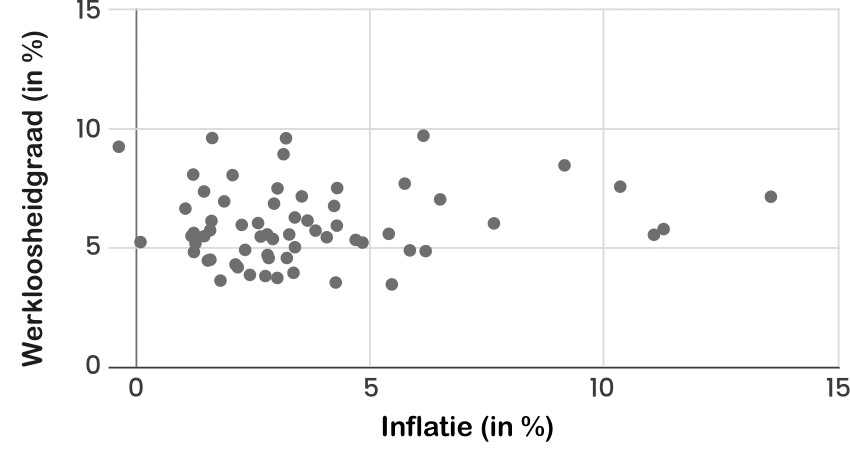
\includegraphics[width=\textwidth]{figures/fig1-1.png}
\caption[Relatie tussen werkloosheid en inflatie]{Relatie tussen werkloosheid en inflatie\index{inflatie}\footnotemark}
\label{fig1}
\end{figure}
\footautocite{11}


Ondanks decennia van opgestapeld bewijs dat het geen accurate verklaring is van hoe de wereld werkt, blijft deze theorie, tot op vandaag, echter bestaan. Rond 1970, toen wereldwijd zowel de inflatie\index{inflatie} als de werkloosheid toenamen, werd de Keynesiaanse trade-off zonder enige twijfel weerlegd. Maar het voordeel van economische wetenschap zonder systematische en herhaalbare methode van experimenteren en testen is dat theorieën na hun weerlegging altijd kunnen worden aangepast op een manier die afwijkende waarnemingen in de echte wereld goed praten. Dat is de essentie van pseudowetenschap.

Hilarisch genoeg pasten de Keynesianen hun theorie aan door er simpelweg een nieuwe term ``aanbodschok'' in op te nemen. Een aanbodschok is een onsamenhangende term, achteraf gemaakt als een rechtvaardiging om te verklaren hoe stijgingen in werkloosheid en inflatie\index{inflatie} tegelijkertijd kunnen voorkomen. Sindsdien zijn de wereldeconomieën getuige geweest van elke denkbare combinatie van inflatie\index{inflatie}- en werkloosheidscijfers, en de Keynesianen hebben met succes de waan in stand gehouden dat er zo’n trade-off tussen werkloosheid en inflatie\index{inflatie} bestaat. Elke afwijking van deze relatie kan worden verklaard door een aanbodschok of diverse andere denkbare substituten te hulp te roepen, en dus is er geen observatie mogelijk die deze relatie weerlegt. Het verklaart alles en verklaart daarom niets. De illusie van economie als een precieze, kwantitatieve en empirische wetenschap wordt alleen in stand gehouden door de theorieën vrij te stellen van empirisch onderzoek in de echte wereld.

\textbf{Na een eeuw natuurkunde te hebben nagebootst en klassieke methodologische grondslagen te hebben losgelaten, is de economie er niet in geslaagd om één kwantitatieve wet of formule te produceren die onafhankelijk getoetst en gerepliceerd kan worden.} Macro-economische formules komen en gaan met de modes van moderne ideologische stromingen, maar geen enkele is objectief gemeten en gerepliceerd op een manier waardoor het een wetenschappelijke wet genoemd kan worden. Dat macro-economie centrale regeringen macht geeft en academici verrijkt, kan helpen verklaren waarom het heeft standgehouden.

\section{Een contrast van benaderingen}

Om de benadering van het menselijk handelen\index{menselijk handelen} van de economische discipline te illustreren en te vergelijken met de moderne kwantitatieve economische methodologie, kunnen we als voorbeeld de kwestie van door de overheid\index{overheid} opgelegde minimumlonen nemen, die een ondergrens opleggen aan wat werkgevers hun werknemers kunnen betalen. Dit is een populaire beleidsinterventie in het grootste deel van de wereld, en de tegengestelde perspectieven hierop dienen als een les binnen de twee verschillende kaders voor het denken over economie: menselijk handelen\index{menselijk handelen} en aggregaten.

Stel je een politicus voor die verkiezingen wil winnen in een land zonder minimumloonwetten. Zoals in alle tijden en plaatsen in de menselijke geschiedenis is er een natuurlijke variatie in de lonen van arbeiders. De politica besluit haar campagne te richten op het verbeteren van de levensstandaard van de armsten uit de samenleving door een minimumloon te verplichten, waarvan ze zich voorstelt dat het de ontvangers ervan een fatsoenlijk bestaan garandeert. Op basis van haar macro-economische raamwerk dat gericht is op aggregaten, besluit de aspirant-leider een minimumloon van \$10 per uur op te leggen. De econoom concludeert dat 20\% van alle werknemers, die 35\% van de bevolking onderhouden, momenteel minder dan \$10 per uur verdienen. Het totale effect van het opleggen van het minimumloon zou leiden tot een loonstijging van \$10 miljard per jaar. Op basis van geavanceerde historische en theoretische modellen schat de econoom verder dat de stijging van de lonen met \$10 miljard zich zou vertalen in een stijging van de consumentenbestedingen met \$8 miljard, waarvan de modellen schatten dat dit zou resulteren in de creatie van 40.000 nieuwe banen, een stijging van de industriële productie\index{productie} met 12\%, een stijging van de export met 4\% en een stijging van het bruto binnenlands product met \$16 miljard.

Volgens deze collectivistische benadering van economische analyse zijn de aggregaten de causale factoren in economische fenomenen, en handelen ze volgens de theoretische relaties die door economen zijn vastgesteld, op een vergelijkbare manier als hoe natuurkundigen en scheikundigen wetenschappelijke regels vaststellen. Deze conclusies zijn tot stand gekomen met behulp van wetenschappelijk ogende vergelijkingen die niet veel verschillen van de vergelijkingen die gebruikt worden in de algemene gaswet. In het kader van de geaggregeerde economische analyse klinkt de wet op het minimumloon als een grote zegen voor de samenleving. De armste werknemers zullen hun levensstandaard aanzienlijk verhogen, sommige werklozen zullen werk vinden als gevolg van de extra uitgaven, en de hele samenleving wordt productiever. Bovendien stijgt de export, wat de economie aan buitenlandse valuta helpt.

Als dit te mooi klinkt om waar te zijn, dan is dat omdat het niet waar is. De dingen zien er anders uit door de lens van de econoom met de Mises-bril. De deugdelijke econoom weet dat menselijk handelen\index{menselijk handelen} de drijvende kracht achter menselijke zaken is en analyseert de wereld niet door middel van geaggregeerde grootheden. In plaats daarvan analyseert hij beslissingen van echte mensen die door deze nieuwe wet worden beïnvloed. Werkgelegenheid is een overeenkomst tussen twee individuen; de werkgever en de werknemer. Een deugdelijk econoom begrijpt dat de keuze van een ondernemer om iemand in dienst te nemen, gebaseerd is op een eenvoudige rekensom: hij zal hem in dienst nemen als zijn bijdrage aan de bedrijfsinkomsten groter is dan zijn loon. Als het wettelijk minimumloon hoger is dan de marginale opbrengst van de werknemer, dan kost het in dienst nemen van de werknemer het bedrijf\index{bedrijf} geld en is het een soort donatie van het bedrijf\index{bedrijf} aan de werknemer. Werkgevers weten dat het aannemen van zo’n werknemer een dure misstap is, en werkgevers die dat niet weten, zullen snel zien dat hun bedrijf\index{bedrijf} failliet\index{faillissement} gaat, omdat het geld blijft verspillen aan lonen die het zich niet kan veroorloven. Alleen werkgevers die deze economische realiteit begrijpen, zullen werkgevers blijven, en zij die dat niet doen, zullen hun bedrijf\index{bedrijf} verliezen. Emotionele chantage door politici kan niets aan deze realiteit veranderen.

Lonen zijn, net als alle prijzen op een markt, niet zomaar willekeurige getallen die door hebzuchtige werkgevers worden gekozen. Ze zijn een weerspiegeling van de marginale productiviteit van de werknemer. Nu de wet bepaalt dat een werknemer \$10 per uur moet krijgen, moet de werkgever opnieuw overwegen of het de moeite waard is om deze werknemer in dienst te nemen. Wanneer de overheid\index{overheid} een minimumloon oplegt, verandert dat niet op magische wijze de calculus van de werkgever, noch verhoogt het op magische wijze de productiviteit van de werknemer. De werkgever zal nog steeds alleen werknemers aannemen wiens productiviteit hoger is dan hun loon. De wet op het minimumloon maakt het dus illegaal voor werkgevers om iemand in dienst te nemen wiens marginale productiviteit minder is dan \$10 per uur. Elke werknemer met een lagere productiviteit zal nu een verlies betekenen voor elk bedrijf\index{bedrijf} dat hem in dienst neemt en hem dat bedrag betaalt. Of hij wordt ontslagen, of het bedrijf\index{bedrijf} dat hem inhuurt, verliest geld en gaat failliet\index{faillissement}. In alle gevallen worden deze banen geëlimineerd, en iedereen met een productiviteit van minder dan \$10 per uur is nu wettelijk werkloos; ofwel werkloos of illegaal tewerkgesteld.

Bekeken door de lens van menselijk handelen\index{menselijk handelen}, is het effect van een minimumloonwet dat het voor werknemers met een lage productiviteit illegaal wordt om een baan te krijgen, en veel van deze werknemers zullen hun baan verliezen. Als we verder kijken door de lens van menselijk handelen\index{menselijk handelen}, dan zien we dat de werknemers die hun baan verliezen de werknemers zijn met de laagste productiviteit in de samenleving, en dit zijn meestal de armste, jongste en minst ervaren werknemers. Door het voor hen illegaal te maken om te werken, wordt het voor hen in feite illegaal om hun productiviteit te verhogen door tijdens het werk te leren en waardevolle werkervaring op te doen. Minimumloonwetten zijn dus bijzonder schadelijk voor de mensen die het meest behoefte hebben aan werk, en ze zijn een factor die bijdraagt aan het ontstaan van grootschalige werkloosheid en ongeschiktheid voor de arbeidsmarkt. Een andere mogelijke implicatie is dat sommige bedrijven, vooral de bedrijven die voor hun bedrijfsvoering afhankelijk zijn van deze laagbetaalde arbeiders, hogere lonen zouden betalen, maar ook de prijzen van hun goederen zouden verhogen om de hogere lonen te financieren. Consumenten zouden dan de prijs\index{prijs} betalen door hogere productprijzen en een lagere hoeveelheid beschikbare goederen. In dit scenario wordt elke potentiële stijging van het inkomen van een werknemer met een laag loon tenietgedaan door een overeenkomstige stijging van de kosten van de goederen die hij moet consumeren.

Al deze gevolgen van minimumloonwetten zijn af te leiden door deugdelijke economen die de loonwet analyseren en de gevolgen ervan voor rationeel handelende individuen evalueren. Dit blijkt een veel nuttigere en nauwkeurigere beoordeling van de situatie te zijn dan alles wat we met wiskundige verhoudingen tevoorschijn kunnen toveren. Prijzen zijn een weerspiegeling van de onderliggende marktrealiteit die door menselijk handelen\index{menselijk handelen} wordt gestuurd. De onderliggende marktrealiteit veranderen door de weerspiegeling ervan te veranderen, werkt niet. Elke poging om prijscontroles door te voeren is mislukt omdat dit soort centrale planning de rol van menselijk handelen\index{menselijk handelen} negeert. Prijscontroles behandelen de economie alsof het over materiële objecten gaat, in plaats van menselijk handelen\index{menselijk handelen}. Schuettinger en Butler hebben een deprimerende, maar onderhoudende geschiedenis van prijscontroles geschreven in \textit{Forty Centuries of Price Controls}, waarin ze illustreren hoe deze exacte dynamiek zich in culturen en naties door de geschiedenis heen heeft herhaald.\autocite{12} Koningen, keizers, politici en bureaucraten zien de wereld van economische transacties als een onmenselijk proces dat ze naar gelang hun behoeften kunnen veranderen. Zij oordelen dat de waarneembare marktverschijnselen binnen aanvaardbare grenzen blijven. Ze gaan ervan uit dat mensen gewoon hun handelen zullen aanpassen om ervoor te zorgen dat deze wetten worden nageleefd. In werkelijkheid passen mensen hun handelingen aan om hun eigen welzijn te optimaliseren, niet om bureaucraten tevreden te stellen. De handelaar verkoopt liever helemaal niet dan met verlies. Je ziet ofwel de vrije marktprijs of je ziet helemaal geen marktprijs. In deze laatste economie komen echte prijzen tot stand op zwarte markten\index{markten}.

Deugende economen begrijpen dat waarneembare economische verschijnselen en statistieken slechts manifestaties zijn van het onderliggende handelen van de betrokken mensen. Mensen proberen voortdurend hun eigen levenssituatie te verbeteren en het is zinloos om hen te verplichten tegen hun eigen belangen in te handelen. Wetten opleggen die tegen het eigenbelang van mensen ingaan, verandert de menselijke natuur niet. Het vermindert de stimulans om zich legaal te gedragen en vernietigt zo het respect van de maatschappij voor wetten. Dit essentiële besef is de reden waarom de deugdelijke econoom voorstander is van individuele economische vrijheid en tegen de beperking ervan door overheden. De menselijke geest is ontembaar en zal niet handelen op een manier die schadelijk is voor zichzelf.

Een goede econoom begrijpt dat mensen voortdurend handelen om hun lot in het leven te verbeteren. Het opleggen van wettelijke straffen op elke vreedzame economische activiteit die ze zouden kunnen kiezen, kan niet leiden tot een verbetering van hun leven, omdat dit simpelweg de keuze aan handelingen die voor hen beschikbaar zijn, zal beperken en verkleinen.

Geaggregeerde analyse verblindt de nepeconoom voor de gevolgen van deze wetten voor de mensen wier vrijheden beperkt worden. Na het formuleren van wiskundige maatstaven voor sociale verschijnselen, neemt de collectivistische econoom vervolgens aan dat deze maatstaven oorzakelijke factoren zijn in het vaststellen van menselijke zaken.

De wereld heeft al veel te veel economische leerboeken die zijn geschreven in de pseudowetenschappelijke kwantitatieve traditie. Dit boek zal daar zeker niet bij horen. Het zal niet proberen om economie uit te leggen in de taal van de natuurwetenschappen, en het zal geen verfijnde aggregaatvergelijkingen bevatten. Dergelijke benaderingen beloven veel, maar leveren weinig betrouwbare, bruikbare inzichten op.

\chapter{Waarde}

\begin{blockquotebox}
    Waarde is dus niet inherent aan goederen. Het is geen eigenschap ervan, noch iets wat onafhankelijk op zichzelf bestaat. Het is een oordeel dat economisch\index{economisch} handelende mensen vellen over het belang van de goederen die ze tot hun beschikking hebben voor het behoud van hun leven en welzijn. Daarom bestaat waarde niet buiten het bewustzijn van mensen.\footnotemark
    \par\raggedleft--- Carl Menger\index{Carl Menger}
\end{blockquotebox}
\autocite{13}

\lettrine{H}et eerste hoofdstuk was een methodologische inleiding tot het onderwerp economie en illustreerde de Oostenrijkse benadering waarin menselijk handelen\index{menselijk handelen} centraal staat. In dit hoofdstuk gaan we in op de kern van het vakgebied economie, de basisbegrippen en de belangrijkste vraagstukken die het vakgebied probeert te beantwoorden.

Aan het einde van de negentiende eeuw legde de Oostenrijkse econoom Carl Menger\index{Carl Menger} de fundamenten voor de moderne economie. Zijn verklaringen over de subjectieve natuur van waarde en economische keuzes, samen met de introductie van marginale analyse, zorgden voor een revolutionaire verandering binnen het domein. Deze concepten boden een stevige theoretische en methodologische grondslag die een systematische analyse mogelijk maakte van de manier waarop mensen economische\index{economisch} beslissingen nemen.\footnote{Nvdr. Economiseren, of economisch\index{economisch} handelen, houdt in dat men bewuste keuzes maakt met het doel middelen optimaal te benutten en een balans te vinden tussen behoeften en de beschikbare middelen.} Dit ondanks het feit dat economie als studiegebied al sinds de tijd van Aristoteles bestond. Mengers baanbrekende werk zorgde voor een dieper inzicht in de impact van economische activiteiten op het menselijk leven. Zijn leerboek \textit{Principles of Economics}, gepubliceerd in 1871, is wellicht het oudste economische leerboek dat vandaag de dag nog steeds van belang en leesbaar is. Dit hoofdstuk biedt een overzicht van enkele kernconcepten uit Mengers werk, waarbij zijn definities worden gebruikt als fundament voor de analyse van thema's die in latere hoofdstukken worden behandeld. Daarna worden de essentiële Mengeriaanse concepten besproken die ten grondslag liggen aan economische analyse: subjectieve waarde\index{subjectieve waarde} en marginale analyse.

\section{Nut en waarde}
\subsection{Goederen}

Menger omschrijft een goed als iets bruikbaars dat ingezet kan worden om menselijke behoeften te bevredigen. Voorwaarden om iets als een goed te beschouwen zijn: ten eerste moet er sprake zijn van een menselijke behoefte; ten tweede moeten de kenmerken van het goed in staat zijn deze behoefte te vervullen; ten derde is het noodzakelijk dat men zich bewust is van deze causale relatie; en ten slotte moet men over het goed kunnen beschikken in voldoende mate om de betreffende behoefte te kunnen bevredigen.

\subsection{Nut}

Nut is het vermogen van een goed om menselijke behoeften te bevredigen. Nut hangt af van ons vermogen om het verband te begrijpen tussen een goed en de behoefte die het vervult. Nut is een algemene voorwaarde om een object een goed te laten zijn. Alleen als iets nut kan bieden, kan het door mensen als een goed worden beschouwd.

\subsection{Schaarste}
Goederen kunnen worden onderverdeeld in twee categorieën, economische en niet-economische. Het onderscheid tussen de twee is \textbf{schaarste\index{schaarste}}: de vraag naar economische goederen is altijd groter dan het geleverde aanbod, terwijl bij niet-economische goederen het aanbod groter is dan de door mensen gevraagde hoeveelheden. 

Een \textbf{niet-economisch\index{economisch} goed} is een goed dat beschikbaar is in hoeveelheden die groter zijn dan de vraag ernaar, waardoor rivaliteit of concurrentie om het goed te bemachtigen uitgesloten is. Het beste voorbeeld is zuurstof, dat essentieel is voor het overleven van de mens, maar desondanks overal waar mensen leven in overvloed aanwezig is.\footnote{Het is schaars bij het onder water duiken en in de ruimte, en daarom wordt het in deze omgevingen een economisch\index{economisch} goed, waarvoor een geavanceerde infrastructuur nodig is om het beschikbaar te maken.} Zuurstof is daarom geen economisch\index{economisch} goed.

Omdat een \textbf{economisch\index{economisch} goed} schaars is, zal de vraag ernaar groter zijn dan het aanbod, en dit creëert rivaliteit om het te verkrijgen, waardoor mensen gedwongen worden om keuzes te maken tussen dit goed en andere goederen. De schaarste\index{schaarste} van economische goederen dwingt mensen om te \textbf{economiseren} en keuzes te maken tussen schaarse alternatieven. Economiseren, of het economisch\index{economisch} handelen, verwijst volgens Menger naar de neiging van mensen om zo groot mogelijke hoeveelheden te hebben van de goederen die hun behoeften kunnen bevredigen, om de nuttige functies van deze goederen te behouden, om hun meest dringende behoeften voorrang te geven boven minder dringende, en om de grootste voldoening te verkrijgen uit de hoeveelheid van een goed.

\subsection{Economie}

Economie is de \textbf{studie van menselijke keuzes bij schaarste\index{schaarste}}. Het richt zich op het analyseren van hoe mensen oplossingen proberen te vinden voor het probleem van het verschil tussen wat ze hebben en wat ze willen, en de gevolgen van hun keuzes. 

Omdat schaarste\index{schaarste} een permanent bestaansgegeven is, maken mensen voortdurend keuzes tussen verschillende manieren van handelen, verschillende goederen en verschillende behoeften om te bevredigen. De noodzaak om deze keuzes te maken dwingt ons om het nut dat we ontlenen aan verschillende goederen tegen elkaar af te zetten, zodat we weloverwogen keuzes kunnen maken.

\subsection{Waarde}

Waarde is onze subjectieve beoordeling van de voldoening die we uit goederen halen, of verwachten te halen. Het stelt ons in staat om economische beslissingen te nemen. Menger definieert waarde als “het belang dat individuele goederen of hoeveelheden goederen voor ons hebben, omdat we ons ervan bewust zijn dat we afhankelijk zijn van de beschikking erover voor de bevrediging van onze behoeften.”\autocite{15} Waarde is volgens Menger ook “het belang dat we eerst toekennen aan het vervullen van onze behoeften, namelijk aan ons leven en ons welzijn en als gevolg daarvan overdragen op economische goederen als de exclusieve oorzaken van de bevrediging van onze behoeften.”\autocite{16}

\subsection{Subjectieve waarde}

De basis van economische analyse, en een van de baanbrekende inzichten uit het werk van Menger, is dat \textbf{waarde subjectief is}. Het bestaat alleen in de geest van de persoon die de waarde bepaalt. Zoals Menger het stelde: “Waarde is dus niet inherent aan goederen, geen eigenschap ervan, noch een onafhankelijk iets wat op zichzelf bestaat. Het is een oordeel dat economiserende mensen vellen over het belang van de goederen die ze tot hun beschikking hebben voor het behoud van hun leven en welzijn.”\autocite{17}

Het is niet een inherente aard van goederen die ze waardevol voor ons maakt, maar alleen onze beoordeling van hun geschiktheid om aan onze behoeften te voldoen. Naarmate hun vermogen om aan onze behoeften te voldoen verandert, verandert ook hun waarde voor ons. Waarde is dus geen fysieke of chemische eigenschap van economische goederen; het is een psychische eigenschap die ze alleen krijgen wanneer mensen ze beoordelen. In de beroemde woorden van Menger: “Waarde bestaat niet buiten het bewustzijn van de mens.”\autocite{18}

Mijn favoriete voorbeeld om de subjectieve aard van waarde te illustreren is olie\index{olie}. Tot in de negentiende eeuw verminderde de aanwezigheid van olie\index{olie} de waarde van een stuk land, omdat de olie\index{olie} eerst weggehaald moest worden voordat het land gebruikt kon worden voor landbouw, handel of woningbouw. Zolang de mens olie\index{olie} als een vervuiling zag, had olie\index{olie} een negatieve economische waarde. Toen mensen zich realiseerden dat geraffineerde olie\index{olie} in een verbrandingsmotor gebruikt kon worden om machines aan te drijven die aan hun behoeften aan transport, elektriciteit en warmteopwekking voldeden, veranderde olie\index{olie} van hinderlijke overlast in een enorm waardevol en essentieel product, waar niemand in de moderne wereld nu zonder kan. Olie in het jaar 2020 verschilt chemisch en fysiek niet van olie\index{olie} in het jaar 1620, en toch is de waarde ervan veranderd van negatief naar positief. Hoewel onze bewuste inschatting van onze behoeften de fysische en chemische eigenschappen van olie\index{olie} niet kan veranderen, kan het de economische waarde ervan wel veranderen. Olie veranderde van een negatieve in een positieve waarde toen het menselijke bewustzijn het als nuttig herkende. Zoals Menger het stelt: “De waarde van goederen vloeit voort uit hun relatie tot onze behoeften, en is niet inherent aan de goederen zelf. Met veranderingen in deze relatie ontstaat en verdwijnt waarde.”\autocite{19}

Om dit punt verder te illustreren: terwijl dit boek in 2020 geschreven wordt, is een aanzienlijk deel van de wereldbevolking onderworpen aan regeringen die in de hele wereld aanzienlijke en verstikkende beperkingen van vrij maatschappelijk verkeer en economische productie\index{productie} opleggen. Olie wordt geproduceerd voor onmiddellijke consumptie\index{consumptie} en er is zeer weinig reservecapaciteit voor de opslag ervan in verhouding tot de enorme verbruikte hoeveelheden. Toen de industrie en het transport vrijwel tot stilstand kwamen, kon de overtollige olieproductie nergens heen, de olieprijs kelderde en werd zelfs een paar dagen negatief. Gezien het grote aanbodoverschot vergeleken met de vraag en het gebrek aan opslagcapaciteit, werd het bezitten van olie\index{olie} weer een last, zoals in het pre-industriële tijdperk, en de eigenaars moesten opnieuw betalen om het kwijt te kunnen. De olieprijs werd al snel weer positief en bleef stijgen. Er veranderde niets aan de inherente eigenschappen van olie\index{olie} toen de prijs\index{prijs} van negatief naar positief naar negatief naar weer positief ging; de omstandigheden van de mensen die de waarde vaststellen veranderden, en zo ook hun subjectieve waarderingen.

Zoals het voorbeeld van olie\index{olie} illustreert, kan waarde niet bestaan buiten de menselijke waardering en keuzes die hun voorkeuren weerspiegelen. Waarde kan geen constante eigenschap van objecten zijn; het is een bewust fenomeen in onze geest. Dit betekent niet dat waarde niet echt is. Waarde is echt en betekenisvol, en zij bepaalt onze handelingen en beslissingen die richting geven aan de productie\index{productie}, consumptie\index{consumptie} en het gebruik van de echte materiële objecten in onze wereld. Mengers erkenning van de subjectieve aard van waarde was een zeer belangrijk keerpunt in het economisch\index{economisch} denken. Economen uit het verleden hadden moeite om uit te leggen hoe goederen gewaardeerd werden en waarom bepaalde goederen waardevoller waren dan andere. Al deze mysteries en paradoxen rondom waardering werden pas opgelost met het Mengeriaanse inzicht van subjectieve waardering en marginale analyse.

\section{Waardering: ordinaal en kardinaal}

De eerste belangrijke implicatie van de subjectieve aard van waarde is dat deze niet objectief gemeten en uitgedrukt kan worden. Aangezien de menselijke beoordeling van waarde subjectief is en voortdurend verandert op basis van onze behoeften en ons begrip van de mogelijkheden van goederen om aan onze behoeften te voldoen, variëren waarderingen van persoon tot persoon; ook veranderen individuele waarderingen voortdurend afhankelijk van individuele omstandigheden. Om enige meting objectief vast te stellen, is een wetenschappelijke eenheid nodig als standaardmaat waartegen verschillende objecten worden beoordeeld, zoals besproken in Bijlage 1.

Gewicht, lengte, temperatuur en andere wetenschappelijke maten worden bepaald in objectief definieerbare eenheden die een nauwkeurige vergelijking tussen verschillende objecten mogelijk maken. Maar een dergelijke eenheid kan niet bestaan voor menselijke waardering, omdat de waarde van een goed geen inherente objectieve eigenschap van het goed is. Het is een subjectieve psychische eigenschap die afhankelijk is van de persoon die de waardering uitvoert, afhankelijk van de steeds veranderende omstandigheden die het nut van dat goed bepalen met betrekking tot het bevredigen van behoeften. Er is geen objectieve standaard waarmee de voldoening van mensen vergeleken kan worden, omdat de individuen zelf de beoordelaars van de waarde zijn. Met andere woorden, er is geen manier om de voldoening die een persoon uit een goed haalt objectief te meten in termen van de voldoening die een andere persoon uit hetzelfde goed haalt.

Zonder een standaard objectieve eenheid is meten onmogelijk, en waardering kan niet worden uitgedrukt in objectieve numerieke \textbf{kardinale} termen, waardoor het onmogelijk is om economische waarde met wiskundige precisie te meten. Zonder een constante eenheid als referentie voor waarde die voor iedereen vast te stellen is, is het niet mogelijk om de economische waarde van verschillende goederen ten opzichte van elkaar uit te drukken. Het is mogelijk om de lengte van verschillende voorwerpen te meten, omdat ze allemaal gemeten kunnen worden aan de hand van de constante referentie van een inch, voet, mijl of meter. Iemand die een koelkast in een keuken wil installeren, kan de toegewezen ruimte van de koelkast meten in centimeters en vervolgens de afmetingen van de koelkast opzoeken om te zien of deze zou passen. Zo’n meting is zinvol en nuttig omdat de klant en de fabrikant van de koelkast een zeer nauwkeurige en precieze gedeelde definitie hebben van wat een centimeter is. Zonder overeenstemming over een gemeenschappelijke constante eenheid zou het onmogelijk zijn om, zonder de koelkast te plaatsen, te weten of hij zou passen.

Zonder een gemeenschappelijke constante eenheid is de enige manier waarop we waarde kunnen uitdrukken \textbf{ordinaal}, waarbij goederen met elkaar worden vergeleken en gerangschikt op basis van de voorkeur van het waarderende individu, maar niet expliciet kwantitatief worden gewaardeerd. Het is mogelijk voor een individu om zijn voorkeur voor het ene goed boven het andere te kennen, omdat er een constante is voor deze vergelijking – het individu dat de waardering doet. Het is dus mogelijk om goederen te \textit{vergelijken} in termen van waarde, aangezien een individu gemakkelijk kan bepalen of hij meer waarde hecht aan goed A dan aan goed B, en meer aan goed B dan aan goed C. Maar deze waardering is puur subjectief, uitgedrukt in verhouding tot het nut dat de persoon die het waardeert, ervaart. Het is onmogelijk voor de persoon om deze voorkeuren in kwantitatieve en kardinale termen uit te drukken, zoals het waarderen van goed A met een precieze numerieke waarde uitgedrukt in dezelfde eenheid waarmee de voorkeur voor goed B wordt uitgedrukt. In de echte economie kan er niet zoiets bestaan als een verklaring die de waarde van goederen weergeeft, zoals \enquote{de waarde van A = 14,372x, de waarde van B = 4,258x, en de waarde van C = 1,273x,} waarbij x een objectieve waarde-eenheid is die gebruikt kan worden voor persoonlijke en interpersoonlijke nutsvergelijkingen.

Zoals Mises het stelt:

\begin{blockquotebox}
    Er is een meer en een minder in het wegnemen van gevoelens van ongemak; maar hoeveel de ene voldoening de andere overtreft, kan alleen maar gevoeld worden; het kan niet op een objectieve manier vastgesteld en bepaald worden. Een waardeoordeel meet niet, het ordent in een schaal van graden, het rangschikt. Het drukt een voorkeursvolgorde uit, maar geen maat en gewicht. Alleen de rangtelwoorden kunnen erop worden toegepast, maar niet de kardinale getallen.\footnotemark
\end{blockquotebox}
\autocite{20}

Denk aan de manier waarop je persoonlijk dingen ten opzichte van elkaar waardeert. Ben je in staat om ze uit te drukken in één eenheid die ze allemaal meet? Kunnen alle dingen die je waardeert, van materiële goederen tot vriendschappen, familie en geluk, gemeten worden in dezelfde eenheid? Bestaat er een vaste wisselkoers\index{wisselkoers} tussen een familielid en materiële goederen? Kun je jouw kind waarderen op basis van een geldhoeveelheid? Hoeveel auto’s heeft een mens nodig om voor zijn kind te ruilen? Menselijke waarden kunnen niet gemeten worden met één gestandaardiseerde eenheid. Menselijke waarderingen kunnen alleen vergeleken worden, maar ze kunnen niet opgeteld, afgetrokken of vermenigvuldigd worden. Zonder een gemeenschappelijke en constante eenheid zijn metingen en wiskundige bewerkingen niet mogelijk.


\section{Waarde en prijs\index{prijs}}

De waarde van economische goederen staat los van hun prijs\index{prijs} en mag hier ook niet mee verward worden. De prijs\index{prijs} van een economisch\index{economisch} goed is niet de objectieve waardering ervan, noch de subjectieve waardering van een van de partijen die handel drijven. De prijs\index{prijs} waartegen een verkoop plaatsvindt, illustreert alleen dat de verkoper het goed minder waardeert dan de prijs\index{prijs}, terwijl de koper het meer waardeert. Als dit niet het geval was geweest, zou de transactie niet hebben plaatsgevonden.

Een veelgemaakte fout in de economie is om waarde en prijs\index{prijs} door elkaar te halen. Die fout gaat gepaard met het idee dat waarde inderdaad objectief gemeten kan worden, uitgedrukt in monetaire eenheden. Maar dat kan niet kloppen, omdat marktprijzen alleen een grens aangeven voor de waarde van goederen, die strikt zijn gebonden aan een bepaalde tijd en plaats. Wanneer iemand ermee instemt om een goed voor \$1.000 te verkopen, geeft ze daarmee aan dat ze het goed op minder dan \$1.000 waardeert. Als ze het voor meer dan \$1.000 had gewaardeerd, zou ze niet geïnteresseerd zijn geweest om het voor \$1.000 te ruilen. Alleen als haar waardering lager is dan \$1.000, zou een bod van \$1.000 haar overhalen om te verkopen. Omgekeerd, als de koper \$1.000 uitgeeft om dat goed te kopen, is het enige dat we over zijn waardering van het goed kunnen zeggen dat die hoger is dan \$1.000, anders zou hij dat bedrag er niet voor betaald hebben. Het is niet mogelijk om de precieze waardering van een individu te bepalen op basis van zijn transactie, maar alleen de boven- of ondergrens ervan. Alleen al de ruil\index{ruil} vertelt ons veel over waardering.

\section{Vrije ruil\index{ruil}}

Wanneer twee mensen er vrij voor kiezen om economische goederen te ruilen, moet het noodzakelijkerwijs waar zijn dat ze allebei geloven dat ze voordeel zullen halen uit de ruil\index{ruil}; anders zouden ze niet ruilen. Wederzijds voordelige ruil\index{ruil} geeft aan dat elke partij iets heeft ontvangen waar ze meer waarde aan hechten dan wat ze hebben opgegeven. De enige manier waarop dit mogelijk is, is als we begrijpen dat ze allebei verschillende subjectieve waarderingen van het geruilde goed hebben. Als de waarde van deze goederen objectief zou zijn, zou deze niet van persoon tot persoon verschillen, en zou de ruil\index{ruil} niet mogelijk zijn, omdat geen van beiden vrijwillig zou kiezen om het goed met de objectieve lagere waarde te accepteren in ruil\index{ruil} voor het goed met de hogere objectieve waarde. Dit wordt meer in detail besproken in Hoofdstuk 9 over handel, waarin de voordelen van ruilhandel\index{ruilhandel} worden geïllustreerd.

\section{Bepalende factoren van waarde}

Het fundamentele verschil tussen economen van de Oostenrijkse School\index{Oostenrijkse School} en andere scholen is dat Oostenrijkers waarde als subjectief beschouwen, terwijl andere scholen waarde als iets objectiefs zien, of objectief meetbaar. Om die schijn in stand te houden, definiëren sommige moderne economieboeken waarde als een functie van nut, wat gemeten wordt in een denkbeeldige en ongedefinieerde eenheid genaamd \textit{util}.\footnote{Nvdr: Nutseenheid} Er is geen standaard voor wat een util is, en geen manier om iets te meten in termen van utils. Sommige moderne wiskundige economen drukken waarde uit in expliciete numerieke termen, gemeten in monetaire eenheden, waarbij ze waarde verwarren met prijs\index{prijs} en niet kunnen verklaren waarom mensen transacties zouden aangaan om voorwerpen te ruilen als beide voorwerpen identieke waarden hebben. Marxisten daarentegen denken dat waarde bepaald wordt door de arbeid die in de productie\index{productie} van een goed gaat zitten. Dit is een absurde stelling volgens welke dingen waardevol worden als er werk in gestoken wordt om ze te produceren, ongeacht of iemand ze wil bezitten. Als je evenveel tijd zou besteden aan het bakken van een normale cake als aan het bakken van een cake van modder, dan zou de marxist beweren dat beide cakes dezelfde waarde zouden hebben.

Er gaat een intuïtieve aantrekkingskracht uit van het idee dat arbeid waarde bepaalt. We kunnen zien dat economische goederen altijd een bepaald element van arbeid vereisen om ze aan de menselijke behoeften te laten voldoen. Zelfs fruit dat in het wild groeit, vereist dat de mens de nodige arbeid verricht om het te plukken en op te eten voordat het aan zijn behoeften kan voldoen. Het is niet mogelijk om goederen te bedenken die menselijke behoeften bevredigen zonder dat er arbeid aan wordt besteed, en dit brengt de aanhangers van de arbeidstheorie tot de conclusie dat het arbeid is die waarde geeft aan goederen en dat waarde gemeten kan worden aan de hoeveelheid arbeid die eraan wordt besteed. Echter, dit is een onhoudbaar idee. 

Men waardeert goederen alleen op basis van hun capaciteit om in onze behoeften te voorzien. Bij een aankoop interesseert de tijd en moeite die in het vervaardigen van een product is gestoken de koper niet; hij kijkt enkel naar de diensten en het nut dat het product voor hem heeft. Producenten zetten arbeid in met de verwachting dat dit de consument waarde zal brengen, maar arbeid leidt niet automatisch tot waardevermeerdering. Arbeid kan men verspillen aan een productieproces\index{productieproces} dat faalt en geen bruikbaar product voortbrengt. De inspanning maakt de output niet waardevol; de nutteloosheid ervan maakt het onwaardeerbaar voor wie de waarde ervan probeert te bepalen. De hoeveelheid arbeid die men in productie stopt, garandeert niet de waarde ervan. Hoewel arbeiders hun arbeid kunnen over- of onderschatten, is het uiteindelijk de keuze van de consument op de markt die de waarde van goederen bepaalt. Producenten en arbeiders investeren hun arbeid in productieprocessen in de hoop waardevolle goederen te creëren. Als de kosten van de inputs lager zijn dan de marktprijs van de output, maakt de producent winst\index{winst}, wat aantoont dat haar investering maatschappelijk productief was omdat de input minder kostte dan de waarde van de output. Echter, als de marktprijs van het product lager is dan de kosten van de inputs, krijgt de producent een signaal dat haar productieproces destructief is, en hoe langer dit doorgaat, des te meer kapitaal\index{kapitaal} ze verspilt.

In de Oostenrijkse School\index{Oostenrijkse School} is waarde subjectief en afhankelijk van het tijdstip en de plaats waarop de waardering plaatsvindt. Waarde wordt afgeleid van menselijke keuzes die noodzakelijk zijn vanwege schaarste\index{schaarste}. Waarde wordt door individuen aan elke eenheid toegekend op het moment en de plaats waarop ze beslissingen nemen, maar het is geen universele eigenschap van het goed. Zonder een subjectieve opvatting van waarde is het niet mogelijk om coherente verklaringen te vinden voor waarom en hoe mensen de economische keuzes maken die ze maken. Hoe consumenten de subjectieve waarde\index{subjectieve waarde} van objecten bepalen, is aan hen. Hetzelfde individu zal hetzelfde goed op verschillende tijden en plaatsen verschillend waarderen, afhankelijk van vele factoren; met name hun bestaande voorraad van dat goed.

\section{Marginalisme}

Mengers andere significante bijdrage aan de economie is het concept van het marginalisme, ook wel bekend als de grensnutschool. Nadat Menger had vastgesteld dat de waarde van goederen niet inherent is aan de goederen zelf, maar eerder subjectief en afhankelijk van hun vermogen om aan onze behoeften te voldoen, paste hij dit toe op de studie van de waarde van verschillende eenheden van hetzelfde goed en legde daarmee de basis voor de moderne economische analyse. 

Aangezien de waarde van goederen wordt afgeleid van hun vermogen om aan onze behoeften te voldoen, en aangezien verschillende voldoeningen een ongelijke waarde voor ons hebben, zal de waarde van verschillende eenheden van hetzelfde goed ook ongelijk zijn, omdat deze afhangt van de behoeften waaraan ze voldoen. Hetzelfde goed zal voor dezelfde persoon een verschillende waarde hebben, afhankelijk van de behoefte waarin het op een bepaald moment voorziet.

Individuen gebruiken de eerste eenheid van een goed om te voldoen aan de belangrijkste en dringendste behoeften die ermee verbonden zijn. Ze zullen de tweede eenheid gebruiken om aan de op één na dringendste behoefte te voldoen. Naarmate de hoeveelheid van het goed dat ze bezitten toeneemt, worden de behoeften waaraan wordt voldaan minder waardevol en minder dringend. Met andere woorden, identieke goederen hebben verschillende waarden voor individuen, omdat het nut dat ze opleveren niet identiek is. De eerste eenheden zijn het waardevolst, en naarmate het aantal geconsumeerde eenheden toeneemt, is elke marginale eenheid minder waardevol dan de vorige.

Menger illustreerde dus dat de waarde die we aan goederen hechten niet afhankelijk is van hun totale of algemene nut en dat hun nut niet iets is dat inherent is aan deze goederen in abstracte zin, ongeacht hun hoeveelheden. Het belang dat we aan goederen hechten is onlosmakelijk verbonden met de hoeveelheid van die goederen, en hun hoeveelheid in verhouding tot het bestaande aanbod van het goed dat we tot onze beschikking hebben. Mensen nemen beslissingen niet op basis van het totale of abstracte nut van een object, maar op basis van het nut dat specifieke hoeveelheden van het goed bieden en hun vermogen om onze verschillende behoeften te bevredigen.

\section{Marginaal nut}

Hoewel Menger de term zelf nooit gebruikte, zou zijn leerling Friedrich von Wieser later de term “marginaal nut\index{marginaal nut}” introduceren om te verwijzen naar het belang dat gehecht wordt aan de minst belangrijke behoefte die door één eenheid van de beschikbare hoeveelheid van een goed wordt verzekerd. Mises definieert het door te zeggen: “We noemen dit gebruik van een eenheid van een homogeen aanbod waarvan de eigenaar `n' eenheden heeft, maar dat aanbod niet zou gebruiken als zijn voorraad één eenheid minder was, `n-1' eenheden, het minst dringende gebruik of het marginale gebruik. Het nut dat ervan wordt afgeleid wordt het marginale nut genoemd.”\autocite{21}

De eerste eenheid voedsel die iemand eet, is bijvoorbeeld extreem waardevol, omdat het het verschil is tussen verhongeren en overleven. De tweede eenheid voedsel zal het verschil zijn tussen louter overleven en goed gevoed zijn. Hoewel het nog steeds zeer waardevol is voor het individu, is de tweede eenheid niet zo waardevol als de eerste. Er zullen nog meer eenheden voedsel worden aangeschaft om van de smaak te genieten of voor sociale bijeenkomsten, die weliswaar waardevol zijn, maar niet zo waardevol als de vorige eenheden die werden gebruikt om te overleven en gezond te blijven. Als de voedselconsumptie van een individu blijft toenemen, komt hij uiteindelijk op een punt waarbij hij geen waarde meer hecht aan een extra eenheid voedsel en het liever niet heeft, zelfs als hij het gratis krijgt aangeboden. Een toename van het aantal geconsumeerde eenheden leidt ertoe dat de eenheden worden ingezet om aan minder dringende behoeften te voldoen, wat betekent dat elke opeenvolgende eenheid een lager nut heeft dan de vorige eenheid en dus een lagere waardering voor individuen. 

Met dit belangrijke inzicht weerlegde Menger het idee dat de waarde van goederen inherent is aan de goederen zelf. Hij illustreerde dat de waarde afhankelijk is van de behoeften waarin de goederen voorzien, die op hun beurt afhankelijk zijn van de overvloed en schaarste\index{schaarste} van de goederen, en alleen voor de persoon die de waarde bepaalt. Niemand wordt ooit gevraagd om het totale aanbod van een goed te waarderen, of om een goed abstract te waarderen. Economische beslissingen hebben alleen betrekking op individuele eenheden van goederen, en individuen nemen op elk moment in de tijd met name beslissingen over de volgende eenheid van een goed dat ze willen consumeren, niet over hun levenslange voorraad ervan, noch over het de abstracte versie van het goed zelf.

\section{Wet van afnemend marginaal nut\index{marginaal nut}}

Een belangrijke implicatie van Mengers benadering van waardering is de wet van afnemend marginaal nut\index{marginaal nut}. Deze wet stelt dat de waardering van een individu en het nut van een goed afnemen naarmate de hoeveelheid van het goed toeneemt. Aangezien individuen de eerste eenheden van een goed dat ze verwerven, gebruiken om de meest dringende behoeften te vervullen waarin het kan voorzien, moet hieruit volgen dat de eerste eenheid van een goed het hoogst gewaardeerd zal worden door dat individu. Naarmate hun bezit van dat goed toeneemt en elke marginale eenheid de minder dringende behoefte vervult, zal elke marginale eenheid een lagere waarde hebben voor het individu. De waarde die iemand aan een goed toekent, hangt op elk moment af van de behoefte die het vervult. Daarom zal de waardering voor iets verminderen naarmate men er meer van verkrijgt.

Dat het marginale nut van een goed afneemt naarmate de hoeveelheid toeneemt, is een belangrijk inzicht in de individuele besluitvorming. Iedereen die wel eens een dure aankoop heeft gedaan, kan zich dit voorstellen. Op de eerste dag dat je een nieuwe auto of nieuw speelgoed hebt, is de nieuwheidsfactor overweldigend en ben je erdoor gefascineerd. Dit wordt na verloop van tijd minder naarmate je meer gewend raakt aan de vele functies en eigenschappen. Wat nieuw was, wordt gewoon en verliest de allure die het had voordat je het ervoer. Je beleeft nog steeds plezier aan het besturen van de auto of het spelen met het speelgoed, maar het specifieke plezier neemt af met elk extra gebruik.

De wet van het afnemende marginale nut herinnert ons er nog eens aan dat er niet zoiets bestaat als een objectieve waarde van goed X, omdat die waarde verandert afhankelijk van de overvloed van goed X en de behoeften die ermee bevredigd worden. Er is altijd alleen een subjectieve waarde\index{subjectieve waarde} van de volgende (marginale) eenheid van goed X voor de persoon die de waarde bepaalt. Dit is afhankelijk van de subjectieve voorkeuren van het individu dat het waardeert en de schaarste\index{schaarste} van het goed.

\section{Waardering door het minst waardevolle gebruik}

Een andere implicatie van Mengers benadering van waardering: als individuen hun inventaris van een goed inzetten om aan hun meest dringende behoeften te voldoen, dan zal hun waardering van de marginale eenheid, hun waardering van de minst belangrijke bevrediging die dit goed verzekert, weerspiegelen. Bij het nemen van aankoopbeslissingen zal de waardering van een goed dus een weerspiegeling zijn van de waardering van de minst belangrijke bevrediging die het goed biedt. Iemand die besluit te betalen voor een maaltijd, zal dit niet betalen op basis van hoeveel waarde hij hecht aan voedsel op zichzelf of hoeveel waarde hij hecht aan al het voedsel dat hij in zijn leven heeft gegeten. Hij zal betalen naar de waarde die hij hecht aan de eerstvolgende maaltijd. De werkelijke waarde van al het voedsel zijn voor de man irrelevant. Als iemand heel zijn leven voldoende voedsel heeft gehad om gezond te blijven en op dit moment een nieuwe maaltijd kan eisen, dan waardeert hij de volgende eenheid voedsel niet net als al het voedsel dat hij tot nu toe heeft gegeten. Hij waardeert het niet alsof het het verschil is tussen leven en dood, want dat is het niet. De beslissing over de volgende maaltijd wordt gewaardeerd op basis van de behoefte die de volgende maaltijd voor deze persoon bevredigt, die, omdat het maar één maaltijd is, aanzienlijk lager zal zijn dan de waarde van voedsel dat hem in het algemeen in leven houdt of de waarde van alle voorgaande maaltijden die hem tot op heden in leven hielden. We kunnen dan zien hoe, wanneer we een keuze moeten maken over een bepaald goed, we het waarderen in het licht van het minst waardevolle gebruik dat mogelijk is, omdat dat de enige marginale keuze is die bestaat. Aan alle waardevollere toepassingen werd al voldaan met eerdere eenheden van eerder genuttigd voedsel. 

De persoon die overweegt om bijvoorbeeld een fles water van een restaurant te kopen, zal niet betalen op basis van de waarde die hij of zij aan water geeft om te overleven of om in zijn of haar dagelijkse basisbehoeften te voorzien. Ze beslissen gewoon over de marginale (volgende) eenheid water die ze gebruiken, nadat ze al andere eenheden water hebben toegewezen aan hun meer dringende behoeften. De prijs\index{prijs} die voor water wordt betaald, komt niet in de buurt van de waarde die het individu aan overleven hecht, omdat de beslissing om een fles water te kopen in een moderne stad alleen betrekking heeft op de consumptie\index{consumptie} van een extra fles water, en niet op overleven. Omdat water essentieel is voor het overleven van de mens, ontstaan alle menselijke samenlevingen alleen op plaatsen waar genoeg water is om aan de essentiële behoeften van de mensen te voldoen. Als deze behoeften verzekerd zijn, zal de prijs\index{prijs} van marginale eenheden niet de waarde van de basisbehoeften weerspiegelen, maar eerder de waarde van de minder dringende behoeften. Dit helpt ons te begrijpen waarom water relatief goedkoop is, ook al is het essentieel. De essentiële aard ervan zorgt ervoor dat mensen er meestal grote hoeveelheden van hebben en hun marginale aankoopbeslissingen baseren op de marginale eenheden die naar minder dringende behoeften gaan.

We kunnen zien waarom goederen die essentieel en belangrijk zijn om te overleven, meestal goedkoop zijn. In de moderne wereld betalen mensen niet voor water op basis van de waarde die ze hechten aan het overleven dankzij dat water. Ze leven al in een tijd en plaats die hun belangrijkste behoeften aan water tegen zeer lage prijzen veilig stelt. Hun individuele aankoopbeslissingen hebben betrekking op het verkrijgen van marginale hoeveelheden water die misschien een lichte dorst kunnen lessen, maar die niet nodig zijn om te overleven of gezond te blijven. Maar als je een individu in een situatie zou plaatsen waarin ze een paar dagen lang niet in staat is om water te kopen voor haar levensbehoeften, dan zou het minst waardevolle gebruik dat het haar zou bieden nog steeds het verschil zijn tussen leven en dood, en dat zou ervoor zorgen dat ze er veel waarde aan hecht. Zoals Mises uitlegt:

\begin{blockquotebox}
    De handelende mens bevindt zich niet in een positie waarin hij moet kiezen tussen al het goud\index{goud} en al het ijzer. Hij kiest op een bepaalde tijd en plaats onder bepaalde omstandigheden tussen een strikt beperkte hoeveelheid goud\index{goud} en een strikt beperkte hoeveelheid ijzer. Zijn beslissing om te kiezen tussen 100 ounce goud\index{goud} en 100 ton ijzer hangt helemaal niet af van de beslissing die hij zou nemen als hij zich in de hoogst onwaarschijnlijke situatie zou bevinden dat hij moet kiezen tussen al het goud\index{goud} en al het ijzer.
    \par\vspace{1em}\noindent
    Wat alleen telt voor zijn feitelijke keuze is of hij onder de bestaande omstandigheden de directe of indirecte voldoening die 100 ounce goud\index{goud} hem zou kunnen geven groter of kleiner acht dan de directe of indirecte voldoening die hij zou kunnen ontlenen aan 100 ton ijzer. Hij spreekt geen academisch of filosofisch oordeel uit over de absolute waarde van goud\index{goud} en ijzer; hij bepaalt niet of goud\index{goud} of ijzer belangrijker is voor de mensheid; hij perverteert niet als schrijver van boeken over de filosofie van de geschiedenis of over ethische principes. Hij kiest gewoon tussen twee voldoeningen die hij niet allebei tegelijk kan hebben.
    \par\vspace{1em}\noindent
    Wanneer de mens geconfronteerd wordt met het probleem van de waarde die moet worden toegekend aan één eenheid van een homogeen aanbod, beslist hij op basis van de waarde van het minst belangrijke gebruik dat hij maakt van de eenheden van het hele aanbod; hij beslist op basis van marginaal nut\index{marginaal nut}.\footnotemark
\end{blockquotebox}
\autocite{23}

\section{Water-diamantparadox}

Een belangrijke uitkomst van Mengers marginale analyse is dat het de eerste economische verklaring bood voor de water-diamantparadox\footnote{Ook bekend als de klassieke waardeparadox.}, een vraagstuk dat economen eeuwenlang had gepuzzeld. Hoe was het mogelijk dat water, onmisbaar voor het menselijk bestaan, vaak zeer goedkoop of zelfs gratis is, terwijl diamanten, die louter luxegoederen zijn en geen essentiële behoefte vervullen, zeer kostbaar zijn? Als waarde werkelijk subjectief is, waarom hechten mensen dan zoveel waarde aan zaken zoals diamanten die ze niet nodig hebben, terwijl ze relatief weinig waarde toekennen aan essentiële zaken zoals water? Zou een arbeidswaardetheorie, die stelt dat diamanten waardevoller zijn omdat hun productie\index{productie} meer arbeid vereist, niet logischer zijn?

Zoals eerder besproken, is de marktwaarde niet gebaseerd op een inherente eigenschap van het goed of de waarde van het totale aanbod; het is gebaseerd op de minst belangrijke behoefte die het goed vervult. Omdat drinkwater doorgaans in overvloed beschikbaar is op plekken waar mensen leven, zijn de meest urgente behoeften aan water al vervuld en worden op de markt beslissingen genomen over eenheden die veel minder dringende behoeften vervullen. Wanneer iemand in een moderne stad besluit geen fles water te kopen, ziet hij af van een kleine, op dat moment minder belangrijke behoefte aan water. Hij heeft nog steeds toegang tot het water dat nodig is voor zijn meest urgente en belangrijkste behoeften, zoals overleven en hygiëne. Diamanten daarentegen zijn uiterst zeldzaam en beschikbaar in zeer beperkte hoeveelheden, en worden aangeschaft door mensen die ze voor hun meest waardevolle doeleinden gebruiken.

Men kan zich een scenario voorstellen waarin zowel water als diamanten uiterst schaars zijn, en de beschikbare marginale eenheden van beide zouden worden ingezet om in de meest urgente behoeften te voorzien. Een persoon die gestrand is in de woestijn en al dagen geen water heeft gedronken, zou bereid zijn veel meer te betalen voor een eerste eenheid water dan voor een eerste eenheid diamant, omdat water in zijn situatie het verschil tussen leven en dood betekent.

Het is daarom niet correct om te stellen dat diamanten waardevoller zijn dan water. De water-diamantparadox benadrukt het belang van de individuele omstandigheden bij het bepalen van de subjectieve waarde\index{subjectieve waarde}. In situaties waarin water overvloedig aanwezig is en diamanten schaars zijn, is water dat gebruikt wordt voor de minst waardevolle doeleinden minder waardevol dan diamanten, waarvan de schaarste\index{schaarste} ervoor zorgt dat zelfs de minst waardevolle doeleinden nog steeds van grote waarde zijn. In situaties waar water schaars genoeg is dat de marginale eenheid gebruikt wordt voor overleving, is water onmiskenbaar waardevoller dan diamanten.

\addtocontents{toc}{\protect\clearpage}
\chapter{Tijd}

\begin{blockquotebox}
    De mens is onderhevig aan de tijd die verstrijkt. De mens wordt geboren, groeit, wordt oud en gaat dood. Zijn tijd is beperkt. Hij moet er zuinig mee omgaan zoals hij zuinig omgaat met andere schaarse factoren. De economisch omgaan met tijd, ook wel bezuinigen genoemd, heeft een bijzonder karakter omdat de tijdsorde uniek en onomkeerbaar is.\footnotemark
    \par\raggedleft--- Ludwig von Mises
\end{blockquotebox}
\footautocite{24}

\section{Het Ultieme Middel}

\lettrine{M}enselijke handelingen vinden plaats door tijd heen. Alle economische
beslissingen vinden plaats op een moment in de tijd, en voor productie
is tijd nodig. Omdat de mens sterfelijk is, is zijn tijd op de aarde
beperkt, en deze beperking maakt het tot een economisch goed en geeft
het waarde. De onomkeerbare aard van de tijd maakt het een uniek
economisch goed. Je kunt de tijd die je aan iets besteedt niet
terugkopen of je tijd oneindig blijven vergroten, zoals dat met andere
goederen wel zou kunnen. Mises en de Oostenrijkse economen schreven
welsprekend over het belang van het begrijpen van de tijdsdimensie van
menselijk handelen en de unieke aard van tijd als economisch goed. Dit
hoofdstuk zal ook voortbouwen op het werk van econoom Julian Simon om te
beargumenteren dat menselijke tijd het ultieme middel is en dat
economische schaarste een gevolg is van de schaarste van menselijke
tijd. Het bezuinigen van tijd is de ultieme economiserende handeling,
waaruit alle economische beslissingen voortvloeien. Als mensen meer tijd
hebben, kunnen ze van elk economisch goed meer maken.\autocite{25} Er zijn
geen bindende fysieke beperkingen op de productie van economische
goederen, en met de inzet van meer menselijke tijd en inspanning kan de
productie van elk goed oneindig worden vergroot. Alleen de schaarste van
tijd dwingt ons om keuzes te maken tussen economische goederen, waardoor
hun schaarste ontstaat.

Wanneer een kind in deze wereld wordt geboren, begint zijn tijd daarin.
Die tijd is onzeker. Het kan maar een uur zijn, maar het kan ook een
hele eeuw duren. Niemand weet hoe lang hij of zij zal leven, maar
iedereen beseft al snel dat het onmogelijk is om eeuwig te leven en dat
zijn tijd alleen maar zal afnemen tot hij helemaal op is. Met dat besef,
en gedurende het steeds volwassener worden, gaan mensen spaarzamer met
tijd om.

In tegenstelling tot de relatieve en voortdurend afnemende schaarste van
materiële voorwerpen, neemt de absolute schaarste van de menselijke tijd
alleen maar toe. Dit is intuïtief waar voor individuen, aangezien groei
en veroudering de mens doet beseffen dat zijn tijd op de aarde alleen
maar beperkter wordt, waardoor hij meer waarde krijgt. Het kan ook
gezien worden in de marktprijs die in de loop van de tijd voor
menselijke arbeid betaald wordt. Naarmate mensen meer tijd besteden aan
werken en productie, vergroten ze de overvloed aan materiële voorwerpen,
waardoor ze in de loop van de tijd in waarde dalen, gemeten in
menselijke arbeid. In zijn boek \textit{The
Ultimate Resource} stelt Simon dat menselijke tijd, of menselijke
arbeid, het ultieme productiemiddel is omdat het gebruikt kan worden om
alle economische goederen en productiemiddelen te maken.\autocite{26}
Het besteden van tijd aan een productieproces zou leiden tot een toename
in het aanbod van de productie, waardoor Simon stelt dat het gebruik van
de term ``resource'' (middel) om materiële goederen te beschrijven een
verkeerde benaming is, omdat materiële middelen de producten zijn van
het inzetten van het ultieme middel, dus menselijke tijd, om materialen
die praktisch oneindig overvloedig zijn om te zetten in bruikbare
economische goederen. De term ``middelen'' suggereert een vaste voorraad
die mensen aanspreken als ze consumeren, maar in werkelijkheid moeten
middelen eerst geproduceerd worden voordat ze geconsumeerd worden, en
hun productie wordt niet beperkt door hun fysieke overvloed op onze
enorme planeet, maar door de hoeveelheid tijd die mensen besteden aan de
productie ervan, en hun opportuniteitskosten gemeten in andere goederen.
Grondstoffen, metalen en brandstoffen worden ons niet als manna uit de
hemel gegeven; ze zijn het complexe resultaat van geavanceerde
productieprocessen om ze te produceren en in te zetten om aan menselijke
behoeften te voldoen.

Simons opvatting van menselijke tijd als het ultieme productiemiddel
verduidelijkt de aard van economische schaarste. Terwijl economen over
het algemeen de schaarste van materiële goederen als uitgangspunt namen
voor economische analyse, zou het nauwkeuriger zijn om schaarste te
begrijpen als een functie van de eindigheid van menselijke tijd. Hoewel
materiële goederen technisch gezien op aarde schaars zijn, liggen hun
absolute hoeveelheden binnen de planeet ver buiten ons vermogen om ze te
gebruiken. De hoeveelheid grondstoffen is daarom niet wat ze schaars
maakt. Wat ze voor ons schaars maakt, is de tijd die nodig is om ze te
produceren, aangezien die voor ons beperkt en begrensd is in een zeer
levendige betekenis.

\section{Opportuniteitskosten}

De schaarste van tijd is de reden waarom mensen niet alleen moeten
nadenken over de directe monetaire kosten van een activiteit, maar ook
over de \textbf{opportuniteitskosten} ervan: de
kosten van een activiteit bestaande uit de niet gerealiseerde waarde van
een andere activiteit die iemand had kunnen kiezen. Het feit dat onze
tijd schaars is, betekent dat we niet alles tegelijk kunnen doen. We
moeten kiezen. Zelfs als fysieke middelen geen beperking zouden zijn, is
de tijd die nodig is om activiteiten uit te voeren altijd een beperkende
factor, en mensen moeten elke keer als ze aan een activiteit deelnemen
rekening houden met de alternatieven die ze er voor opgeven.

De onvermijdelijkheid van de dood en de eindigheid van tijd, en dus de
schaarste ervan, maken een constante afweging van opportuniteitskosten
noodzakelijk, en daaruit komt al het economisch denken en handelen van
de mens voort. Alle menselijke handelingen verbruiken tijd en gaan
daarom ten koste van niet gekozen handelingen. Als we schaarste in het
algemeen begrijpen als een gevolg van de schaarste van tijd, begrijpen
we ook de opportuniteitskosten en waarom de economische manier van
denken altijd de kosten van het niet gekozen alternatief moet omvatten.
Omdat menselijke tijd schaars is, is hij waardevol voor mensen. Er is
dus altijd een alternatief waardevol tijdsgebruik beschikbaar voor een
individu, waarmee rekening gehouden moet worden.

\section{Materiële Overvloed}

De meest gebruikelijke maatstaf om de overvloed aan grondstoffen te
bespreken is de bewezen reserve, die verwijst naar de hoeveelheden van
een grondstof waarvan definitief bekend is dat ze op bepaalde locaties
voorkomen en die met de huidige technologie en prijzen gewonnen kunnen
worden.\autocite{27}

Volgens deze maatstaf is de voorraad voor elk bekende natuurlijke
hulpbron op de lange termijn toegenomen. Naarmate we meer van een
grondstof verbruiken, wordt deze ingezet voor meer doeleinden, en dat
creëert meer vraag ernaar, waardoor er meer naar gezocht wordt en de
reserves dus toenemen. Simon illustreert hoe de bewezen reserves tussen
1950 en 1990 zijn toegenomen voor een aantal belangrijke industriële
metalen. De wereldbevolking bedroeg in 1950 ongeveer 2,5 miljard mensen,
en was in 1990 gegroeid tot ongeveer 5,32 miljard
mensen.\autocite{28} Gemeten in dollars van 2011, werd het wereldwijde bbp in 1950
geschat op \$9.250 miljard, en in 1990 op \$47.040
miljard.\autocite{29} Dus in een periode van veertig jaar waarin de
menselijke bevolking met een factor 2,13 groeide en waarin de menselijke
productie vervijfvoudigde, groeiden de bewezen reserves van de meeste
metalen met hogere snelheden dan de bevolkingsgroei, in plaats van
uitgeput te raken. De bewezen reserves van lood groeiden met een factor
3, zink met 4,21; koper met 5,66; ijzererts met 8,27; olie met 13,1;
fosfaat met 14 en bauxiet met 16,6.\autocite{30}

Het is duidelijk dat de bewezen reserves geen redelijke maatstaf zijn
voor de totale hoeveelheid grondstoffen op aarde, maar eerder een
maatstaf voor de hoeveelheid moeite die we doen om grondstoffen te
zoeken en te exploreren. Bewezen reserves zijn een maatstaf voor de
hoeveelheid grondstoffen die we zoeken met de huidige technologieën
tegen de huidige prijzen. Naarmate we van deze middelen gebruikmaken en
onze levensstandaard stijgt, ontwikkelen we betere technieken om te
graven, en delven we in meer gebieden, waardoor deze bewezen reserves
groeien. Bewezen reserves zijn slechts het topje van de reusachtige,
deels verborgen ijsberg van de totale voorraad grondstoffen van de
aarde, die we nooit met enige nauwkeurigheid kunnen schatten. De aarde
is enorm groot en de exacte samenstelling ervan is zeer moeilijk vast te
stellen vanaf het oppervlak. De hele aarde opgraven om een sluitende
inventarisatie te maken is een zinloze en onmogelijk dure klus die
niemand ooit serieus zou kunnen overwegen.

Het helpt om een idee te krijgen van de omvang van de aarde om Simons
bewering te volgen. De oppervlakte van de aarde is 510,1 miljoen km², en
de totale oppervlakte die tussen 2000 en 2017 voor mijnbouw werd
gebruikt, werd geschat op 57.277 km², oftewel 0,011\% van de oppervlakte
van de planeet.\autocite{31} Als de
aarde de grootte van een voetbalveld had (105m × 68m, oftewel 7140 m²),
zou de oppervlakte van alle mijnen ter wereld 0,785 m² zijn, ongeveer de
grootte van een klein bureau (een bureau van 122 cm × 61 cm heeft een
oppervlakte van 0,744 m²).

\textbf{Figuur 2.} Als de aarde een voetbalveld was, zouden alle mijnen
een klein bureau zijn

De diameter van de aarde is 12.742 kilometer. Daarentegen is de diepste
mijn ter wereld, de Mponeng goudmijn nabij Johannesburg, \enquote{slechts} 3,16 km
tot 3,84 km diep, oftewel 0,024\% tot 0,03\% van de diameter van de
aarde. Ter vergelijking: als de aarde een bal was met een diameter van 1
meter, zou het diepste gat dat ooit in de aardkorst is gegraven 0,027 cm
diep zijn, minder dan de dikte van drie pagina's van dit boek. Het
overgrote deel van het aardoppervlak is tijdens de zoektocht naar
grondstoffen niet afgegraven en op de weinige plekken waar we wel hebben
gegraven, hebben we letterlijk nauwelijks een schrammetje in het
aardoppervlak gemaakt. Alle grondstoffen die de mensheid in duizenden
jaren van consumptie en exploitatie heeft gebruikt, zijn slechts een
fractie van de overvloed die beschikbaar is in de oppervlakkige 0,027\%
van de diameter van de Aarde.

De meeste mijnen zijn rond de 300 meter diep. Laten we bij het volgende
punt uitgaan van een zeer royale gemiddelde diepte van een mijn van 1
km. Dit zou betekenen dat het totale volume aan mijnen in de periode
tussen 2000 en 2017 57.277 km\textsuperscript{3} was. Het volume van de aarde is
1.083.206.916.845,80 km³ (ongeveer een triljoen kubieke kilometer). Het
volume van alle mijnen op aarde is dus 0,00000529\% van het volume van
de aarde. Met andere woorden, de aarde is 18.911.725,8 keer zo groot als
alle mijnen die erop liggen en waaruit we al onze grondstoffen hebben
gehaald. Ter vergelijking, als het volume van de aarde dat van een
olympisch zwembad was, dan zouden alle mijnen ter wereld ruwweg de
grootte van een half glas hebben.\autocite{32}

\textbf{Figuur 3}. Als de aarde een olympisch zwembad was, zouden al
onze mijnen een half glas zijn

Als alle grondstoffen die mensen verbruiken afkomstig zijn uit het
equivalent van een half glas van het olympische zwembad dat de aarde is,
dan wordt het duidelijk waarom het zorgen maken over de totale
hoeveelheid grondstoffen zo misplaatst is. Als acht miljard mensen
kunnen leven van het equivalent van een half glas uit een Olympisch
zwembad, dan is het duidelijk dat de totale hoeveelheid water in het
zwembad irrelevant is voor het menselijk leven en alle economische
overwegingen. De wereldbevolking zou moeten verdubbelen om uit een
olympisch zwembad de waarde van één glas te moeten produceren. Zelfs met
een enorme groei van de wereldbevolking zullen we nauwelijks een krasje
op het oppervlak van onze enorme, overvloedige planeet maken. Zelfs de
meest conservatieve schattingen komen tot de conclusie dat de totale
overvloed in de aardkorst van een bepaalde natuurlijk voorkomende
grondstof vele ontelbare veelvouden is van de totale hoeveelheid die
mensen ervan consumeren en die hoeveelheid vormt geen relevante limiet
of bindende beperking voor ons consumptieniveau. Het is heel
waarschijnlijk dat de totale overvloed in de aardkorst van een bepaald
metaal gelijk is aan miljoenen jaren menselijke consumptie. Zelfs als de
huidige, verondersteld niet-duurzame, consumptietrends duizenden jaren
zouden aanhouden, zouden we niet in staat zijn om de volledige inhoud
van de aarde aan een bepaald metaal op te maken. De limiet en beperking
op de hoeveelheid die we in een bepaald jaar van elk metaal kunnen
produceren, blijft de hoeveelheid tijd en middelen die we besteden aan
de productie ervan en de hoeveelheid andere goederen en diensten die we
bereid zijn op te geven voor de productie ervan.

Afgezien van het feit dat ze als illustratie in dit economieboek worden
gebruikt, zijn deze geaggregeerde metingen van de grondstoffen op aarde
volledig zinloze en irrelevante meetgegevens die geen rol spelen in de
economische beslissingen die waar dan ook door wie dan ook worden
genomen. Er zijn geen economische beslissingen die betrekking hebben op
de totale voorraad metaal op de aarde, en alle individuele economische
beslissingen met betrekking tot een middel worden in de marge gemaakt,
gebaseerd op de volgende marginale eenheid land die geëxploiteerd moet
worden, de marginale kosten van het winnen van de volgende eenheid, en
de marginale opbrengst die verwacht wordt van de verkoop ervan. Op geen
enkel moment kan een individu of entiteit een economische beslissing
nemen die betrekking heeft op de totale geaggregeerde voorraad van een
materiaal op aarde. Economische berekeningen worden voortdurend in de
marge gemaakt en hebben alleen betrekking op schaarse grondstoffen die
opportuniteitskosten met zich meebrengen. Mineralen in de aardkorst zijn
niet schaars en bieden geen nut voor mensen. Om er daarentegen bruikbare
materialen van te maken, moeten er echte beslissingen genomen worden
over de toewijzing van marginale eenheden van schaarse grondstoffen aan
de exploratie-, opgravings-, extractie-, raffinage- en
productieprocessen.

Een nuttige analogie hierbij is om de grondstoffen van de aarde te zien
als stenen, en onze consumptie van grondstoffen als het gebruik van
stenen om huizen te bouwen. Geen enkele economische beslissing hoeft
rekening te houden met de totale hoeveelheid stenen op aarde;
economische beslissingen hebben alleen betrekking op de toepassing van
schaarse middelen, arbeid, kapitaal en land, op het proces van het
delven en toepassen van stenen. Het zou krankzinnig zijn voor een
huizenbouwer om zich bezig te houden met de beschikbaarheid van stenen
in de natuur, als al onze huizen een oneindig klein deel van de stenen
op aarde nodig hebben voor de bouw ervan. De enige economisch dringende
zorg voor de huizenbouwer is of hij aan de menselijke arbeid en het door
mensen geproduceerde kapitaal kan komen dat nodig is om die stenen in
huizen om te zetten.

Waar we echt waarde aan hechten zijn niet de grondstoffen, maar
economische goederen die van grondstoffen gemaakt zijn. Daar is tijd
voor nodig, en dat is wat schaars is. Dat is de schaarste waaruit alle
andere schaarste voortkomt. De ruwe materie bestaat overal om ons heen,
maar de tijd om er economische goederen van te maken is schaars. Mensen
zijn geen passieve ontvangers van manna dat op kan raken. Mensen zijn de
producenten van al deze middelen, en wanneer de vraag naar deze
materialen toeneemt, is het handelen van de mensen die ze produceren en de
prikkels waarmee ze te maken krijgen, de belangrijkste bepalende factor
voor hun schaarste. Naarmate de vraag naar een natuurlijke hulpbron
toeneemt, worden ze gestimuleerd om er meer van te produceren en meer in
de productie ervan te investeren. Naarmate de productiviteit toeneemt,
zijn we in staat om grotere hoeveelheden van het aanbod van het goed te
verkrijgen per hoeveelheid tijd die in de productie ervan wordt
geïnvesteerd, wat betekent dat de reële prijs van het goed, gemeten in
menselijke arbeid, zal blijven dalen. Dit feit wordt bevestigd door
tientallen jaren van gegevens over de grondstoffenmarkt.

Hoewel grondstofprijzen kunnen stijgen in nationale valuta en dat
meestal ook doen, is dat het gevolg van de devaluatie van nationale
valuta. Gemeten aan de loonkosten, of de prijs van menselijke tijd,
dalen de prijzen van alle grondstoffen op de lange termijn, zelfs als de
consumptie gestaag toeneemt. In een wereld met hard geld, zoals onder de
goudstandaard, zou het volkomen normaal zijn om te verwachten dat de
prijzen van alle grondstoffen in de loop van de tijd consequent dalen,
met slechts af en toe een tijdelijke stijging door scherpe, plotselinge
dalingen in het aanbod en de onderbreking van de productie. Goud, of wat
er ook als geld wordt gebruikt, zou altijd het goed zijn waarvan het
aanbod het langzaamst toeneemt, waardoor de eigenaars ervan er voor
altijd meer van alle andere goederen kunnen krijgen, waarvan het aanbod
sneller toeneemt.

Economen Gale Pooley en Marian Tupy hebben ter ere van Julian Simon een
economische index gemaakt die de prijzen van 50 basisproducten meet in
``loon''. Zij ontdekten dat de tijd die nodig is om een mandje van 50
basisproducten te verdienen in de periode tussen 1980 en 2020 met 75,2\%
is gedaald, wat betekent dat een uur werk in 2020 4,03 keer zoveel van
de 50 basisproducten kan kopen als in 1980, wat een jaarlijkse groei van
3,55\% en een verdubbeling van de overvloed aan basisproducten elke 20
jaar betekent.\autocite{33} Hoewel de menselijke bevolking in deze
40 jaar met 75,8\% is toegenomen, decennia die de grootste
bevolkingsgroei en de hoogste consumptie en levensstandaard in de
geschiedenis kenden, zijn de prijzen van 50 basisproducten met driekwart
gedaald, gemeten in arbeidstijd die nodig is om ze te kopen. Deze
gegevens kunnen alleen begrepen worden in de context van een oneindig
grote aarde waarvan de fysieke grenzen niet in de buurt van onze greep
liggen, een greep die beperkt wordt door de schaarste van onze tijd en
de opportuniteitskosten die gepaard gaan met het verhogen van de
productie van een bepaalde natuurlijke hulpbron.

\textbf{Figuur 4}. Veranderingen van prijzen gemeten in tijd en
overvloed van 50 basisproducten (1980 tot 2020)

De enige schaarste, zoals Julian Simon op een briljante manier heeft
aangetoond, is de tijd die mensen hebben om deze goederen te produceren,
en daarom blijven de lonen wereldwijd stijgen, waardoor producten en
materialen voortdurend goedkoper worden als we ze meten in menselijke
arbeid. De enige `grondstof' waarvan de prijs in de loop van de
geschiedenis bijna voortdurend is gestegen, is menselijke tijd, zoals we
zien als we naar lonen kijken. Naarmate we meer inventieve manieren
blijven vinden om de productie van fysieke hulpmiddelen te verhogen,
blijft hun reële prijs, in menselijke tijd dalen, terwijl de waarde van
menselijke tijd blijft stijgen. Alleen met dit raamwerk kan men
begrijpen waarom de mensheid nog nooit zonder grondstoffen is komen te
zitten, zelfs niet na vele millennia van exploitatie van de aarde en de
niet aflatende voorspellingen van naderend onheil door uitputting van
natuurlijke hulpbronnen. Niet alleen is geen enkele grondstof uitgeput
geraakt, maar in feite blijven de reële prijzen dalen, blijft de
jaarlijkse productie van vrijwel alle grondstoffen elk jaar stijgen, en
zijn de bewezen reserves van elke grondstof in de loop van de tijd
alleen maar toegenomen terwijl onze consumptie is gestegen, zoals
hierboven in de gegevens van Simon wordt vermeld. Als grondstoffen als
eindig moeten worden beschouwd, dan zouden de bestaande voorraden in de
loop van de tijd afnemen naarmate we meer consumeren. Maar zelfs als we
altijd meer verbruiken, blijven de prijzen dalen, en de technologische
verbeteringen voor het vinden en opgraven van grondstoffen stellen ons
in staat om meer ongebruikte voorraden te vinden.

Olie, het onmisbare smeermiddel van moderne economieën, is het beste
voorbeeld omdat er vrij betrouwbare statistieken voor zijn. Zoals Figuur
5 laat zien, blijven het olieverbruik en de olieproductie van jaar tot
jaar stijgen, terwijl de bewezen reserves nog sneller toenemen. Volgens
gegevens van BP's Statistical Review of World Energy lag de jaarlijkse
olieproductie in 2015 46\% hoger dan in 1980, terwijl het verbruik 55\%
hoger lag. De oliereserves daarentegen zijn met 148\% toegenomen,
ongeveer het drievoudige van de toename in productie en verbruik.

\textbf{Figuur 5.} Olieverbruik en bewezen reserves\autocite{34}

Vergelijkbare statistieken kunnen worden opgesteld voor grondstoffen die
in verschillende hoeveelheden voorkomen in de aardkorst. De zeldzaamheid
van een grondstof bepaalt de relatieve kosten om deze uit de aarde te
halen. Meer voorkomende metalen, zoals ijzer en koper, zijn gemakkelijk
te vinden en daardoor relatief goedkoop. Zeldzamere metalen, zoals
zilver en goud, zijn duurder. De limiet op hoeveel we van elk van deze
metalen kunnen produceren blijft echter de opportuniteitskosten van hun
productie vergeleken met elkaar, in subjectieve menselijke waardering,
en niet hun absolute hoeveelheid. Er is geen beter bewijs hiervoor dan
het feit dat goud, één van de (al dan niet) zeldzaamste metalen in de
aardkorst, al duizenden jaren wordt gedolven en nog steeds in steeds
grotere hoeveelheden wordt gedolven naarmate de technologie
voortschrijdt.

\textbf{Figuur 6.} Wereldwijde jaarlijkse goudproductie\autocite{35}

Als er andere metalen zijn die zeldzamer zijn dan goud, dan zijn die
allemaal recent ontdekt en hebben we niet zoveel tijd besteed aan het
vinden van hun reserves en het aanleggen van hun voorraden als bij goud.
Maar goud wordt al duizenden jaren naar gezocht en gedolven, en de
jaarlijkse productie ervan stijgt elk jaar, dus het heeft geen zin om in
praktische zin te spreken van een natuurlijk element dat beperkt is in
zijn hoeveelheid. Schaarste is alleen relatief ten opzichte van
materiële hulpmiddelen, waarbij de verschillen in de delvingskosten de
schaarste bepalen.

\section{Simons Weddenschap}

Nadat de Amerikaanse president Richard Nixon in 1971 de inwisselbaarheid
van de Amerikaanse dollar in goud opschortte, begonnen alle prijzen
onverbiddelijk te stijgen, een trend die tot op de dag van vandaag
aanhoudt. Voor mensen die in de jaren 70 gewend waren aan relatief
stabiele prijzen onder de goudstandaard, leken deze prijsstijgingen een
teken van een economische apocalyps, omdat ze de indruk wekten dat al
onze kostbare grondstoffen uitgeput raakten. Terwijl de wereld werd
meegesleurd in de hysterie over de uitputting van grondstoffen en
overbevolking, was Simon niet tevreden met alleen maar schrijven om de
hysterie tegen te gaan. Hij probeerde de leegheid van de hysterici bloot
te leggen door Paul Ehrlich, een van de meest vooraanstaande hysterici
van de twintigste eeuw, uit te dagen voor een openbare weddenschap over
de kwestie.

Ehrlich had een groot aantal hysterische tirades gepubliceerd die het
niet waard zijn om in de bibliografie van dit boek opgenomen te worden,
waaronder de voorspelling dat verschillende essentiële hulpbronnen voor
de mensheid uitgeput zouden raken als gevolg van overbevolking, en
voegde daar typisch misantropische tirades over eugenetica en gedwongen
sterilisatie en andere maatregelen om de menselijke bevolking te
verminderen aan toe. Simon daagde Ehrlich uit om grondstoffen te noemen
waarvan hij zeker wist dat ze op zouden raken of veel schaarser zouden
worden over een periode langer dan een jaar, en Simon zou met hem om
\$1.000 wedden dat elk van deze grondstoffen aan het einde van de
periode reëel gezien daadwerkelijk goedkoper zou zijn.

De weddenschap moet voor Ehrlich als een gift hebben geleken, zo
overtuigd was hij van zijn waarschuwingen over de dreigende uitputting
van kritieke grondstoffen. Ehrlich noemde 5 metalen en een periode van
10 jaar om hun prijs vast te stellen, van 1980 tot 1990. Aan het einde
van de periode was elk van deze metalen reëel gezien goedkoper dan aan
het begin. Dertig jaar later zijn deze metalen alleen maar goedkoper
geworden, terwijl hun jaarlijkse productie elk jaar blijft stijgen.

De reden dat de prijs van al deze metalen daalde, is dat hun schaarste
relatief is, niet absoluut. Ze zijn schaars voor ons omdat de tijd en
middelen die nodig zijn om ze te produceren, moeten worden onttrokken
aan de productie van andere grondstoffen. Simon begreep dat naarmate de
menselijke bevolking toenam en de vraag naar deze metalen steeg, er meer
middelen aan de productie van deze metalen besteed zou worden, de
hoeveelheden zouden toenemen en de prijzen zouden dalen. De stijging van
de vraag zorgt voor een stijging van de prijzen, waardoor de producenten
van deze metalen meer winst maken, meer geld hebben om te investeren en
meer investeringen kunnen aantrekken. Deze investeringen gaan naar het
opsporen, winnen, raffineren en distribueren van de metalen, wat
allemaal leidt tot een stijging van de productiviteit, de productie per
eenheid input. Zoals meer in detail besproken zal worden in Hoofdstuk 4,
maken grotere kapitaalinvesteringen het mogelijk om complexere en
langere productiemethoden te gebruiken die een hogere productiviteit per
werknemer opleveren.

Als geoloog was Ehrlichs beeld van schaarste gebaseerd op schattingen
van de consumptie ten opzichte van de reserves, zonder rekening te
houden met de rol van menselijk handelen in het teweegbrengen van
veranderingen in deze getallen. Ehrlich vergeleek in werkelijkheid de
bewezen reserves van metalen met hun jaarlijkse consumptiecijfers en
schatte het aantal jaren waarin de mensheid door haar reserves heen zou
raken. Simon begreep als econoom de dynamiek achter de productie van
deze metalen, ook al was hij nauwelijks bekend met de geologische
realiteit. Door economie op te vatten als de studie van menselijk
handelen, zoals besproken in Hoofdstuk 1, wist Simon dat de schaarste
van deze metalen uiteindelijk afhing van de hoeveelheid tijd die mensen
eraan besteedden, en dat was weer afhankelijk van de stimulans die
mensen hadden om deze hulpbronnen te produceren, niet van geologische
beperkingen. Als de vraag naar een metaal toeneemt, is er geen beperkte,
uit te putten voorraad. Er zijn altijd andere gebieden om te exploreren
en diepere mijnen om te graven.

\section{Tijdsvoorkeur}

Omdat de menselijke tijd eindig en onzeker is, weet niemand met
zekerheid hoe lang hij zal leven of wanneer hij zal sterven. Dit creëert
in de mens een \textbf{tijdsvoorkeur}, een universele voorkeur voor
vroegere boven latere voldoening van behoeften. Mensen consumeren of
hebben een goed altijd liever vandaag dan in de toekomst, omdat
overleven nooit zeker is. Tijdsvoorkeur is altijd een positieve waarde,
wat betekent dat het nut van vandaag altijd de voorkeur heeft boven
hetzelfde nut van morgen. Mensen beschikken ook liever vroeger dan later
over hun middelen, omdat ze, in het geval van duurzame goederen,
waarschijnlijk langer van hun diensten zullen genieten naarmate ze deze
eerder ontvangen.

Hoewel tijdsvoorkeur altijd positief is, varieert de waarde ervan
afhankelijk van de mate waarin mensen toekomstig nut negeren ten
opzichte van huidig nut. Een relatief lage tijdsvoorkeur duidt op een
lage mate van het negeren van toekomstig nut, wat duidt op een relatief
grotere bezorgdheid over de toekomst. Een hogere tijdsvoorkeur duidt op
een hogere mate van negeren van toekomstig nut, een relatief lagere
bezorgdheid over de toekomst en een sterke gerichtheid op het heden.

\section{Tijd Economiseren}

Zoals hierboven besproken is economische schaarste uiteindelijk de
schaarste van menselijke tijd. We kunnen dan ook begrijpen dat het hele
menselijke economiseren draait om het economiseren van tijd. Dat wil
zeggen, we proberen de hoeveelheid en subjectieve waarde van onze tijd
op aarde te vergroten. Dat tijd schaars is, betekent dat mensen
voortdurend proberen om er zuiniger mee om te gaan en het te besteden op
manieren die hen de meeste voldoening geven of die het meest waardevol
zijn. Omdat de toekomst onzeker is en tijdsvoorkeur universeel positief
is, proberen mensen voortdurend de waarde van hun huidige tijd te
maximaliseren. 

\textbf{Vrije tijd} is de term die wordt gebruikt om de
tijd aan te duiden die mensen besteden aan dingen die ze leuk vinden
omwille van zichzelf, dingen die hen onmiddellijk plezier opleveren, in
tegenstelling tot dingen die ze doen in ruil voor een toekomstige
beloning of voldoening. Vrije tijd is wat economen goede tijden noemen.
Iedereen heeft het graag naar zijn zin. Het leven is eindig en mensen
willen het natuurlijk liever besteden aan dingen die ze leuk vinden dan
aan dingen die ze niet leuk vinden. Tijdsvoorkeur zal met andere woorden
altijd positief zijn.

Iedereen zou het liefst zijn hele leven in vrije tijd doorbrengen. Maar
omdat we geen eeuwige wezens zijn die in de Hof van Eden leven, zal te
veel vrije tijd onvermijdelijk een vroege dood door honger of de
krachten van de natuur betekenen. We kunnen ook niet eindeloos van onze
vrije tijd genieten, want we zijn altijd in staat om manieren te
bedenken waarop we de kwaliteit en kwantiteit van onze tijd op de aarde
kunnen verbeteren. Het is niet alleen de waarde van het `nu' die mensen
proberen te optimaliseren. We willen ook de hoeveelheid tijd die we op
de aarde hebben maximaliseren; met andere woorden, proberen lang te
leven en niet vroeg te sterven. We willen ook de waarde van onze
toekomstige tijd maximaliseren. Het menselijk verstand stelt ons in
staat om manieren te bedenken waarop we kunnen handelen om onze
overlevingskansen te vergroten en om voor onze toekomst te zorgen.
Menselijk verstand stelt ons in staat om ons een betere toekomst voor te
stellen, om ervoor te werken, en om huidig genot ervoor op te offeren.
Menselijk verstand stelt ons ook in staat om ons de gevolgen voor te
stellen als we er niet in slagen om voor de toekomst te zorgen, en om
deze met andere handelingen te vergelijken. Mensen kunnen elke minuut
van hun leven doorbrengen met alleen maar om het heden te geven, maar ze
zouden uiteindelijk in een zeer onzeker heden terechtkomen, omdat ze er
in het verleden niet voor gezorgd hebben. Hoe meer waarde een individu
aan de toekomst hecht en hoe meer hij werkt en ervoor zorgt, hoe groter
de kans dat hij in de toekomst zal overleven.

\textbf{Uiteindelijk is dé economische vraag hoe we huidig nut afwegen
tegen langer overleven en toekomstig nut. De belangrijkste ruil die een
individu doet, is de ruil met zijn toekomstige zelf.} De eenvoudigste
ruil is die waarbij men afziet van onmiddellijk plezier ten gunste van
arbeid om voor de toekomst te zorgen. Terwijl iemand van zijn heden
geniet, zal hij behoefte hebben aan voedsel en onderdak, op het meest
basale niveau. Maar voedsel moet op worden gejaagd, worden verbouwd of
verkregen, en onderdak moet gebouwd of verkregen worden. Dat vereist het
opofferen van huidig genot ten gunste van arbeid.

De mens zijn rede doet hem inzien dat hij voor zijn toekomstige zelf kan
zorgen en zijn overlevingskansen kan vergroten. Hij begrijpt dat arbeid,
hoewel het op het moment zelf onaangenaam is en de kosten met zich
meebrengt om plezier te moeten missen, hem in staat zal stellen om in de
toekomst de vruchten ervan te plukken. Het verstand en het verlangen om
lang en goed te leven, spannen samen om de tijdsvoorkeur van de mens te
verlagen. Ze roepen hem niet alleen op om zijn vrije tijd op te geven
voor het ongerief van werk, maar ook om voor zijn toekomst te zorgen
door huidige consumptie uit te stellen, voor de toekomst te sparen en
duurzame goederen en productief kapitaal te vergaren.

Het is dit proces van het verlagen van de tijdsvoorkeur,
toekomstgerichtheid en voorzorgsmaatregelen dat het beschavingsproces in
gang zet. Of, zoals Hans-Hermann Hoppe het formuleerde: \enquote{zodra het laag
genoeg is om überhaupt te sparen en kapitaal of duurzame
consumptiegoederen voort te brengen, wordt een tendens naar een daling
van de tijdsvoorkeur in gang gezet, die gepaard gaat met een
`beschavingsproces.'}\autocite{36}

Naarmate mensen de vruchten plukken van voorzieningen voor de toekomst
en een lage tijdsvoorkeur, zullen ze er vaker voor kiezen. Werk en de
accumulatie van kapitaal leiden tot een hogere productiviteit, waardoor
de waarde van de tijd van een individu toeneemt. Hoe meer mensen in
staat zijn om voor hun toekomst te zorgen, hoe minder onzeker die
toekomst wordt, wat op zijn beurt weer aanzet tot verdere zorg voor de
toekomst, sparen, kapitaalopbouw en een waarschijnlijke toename in de
hoeveelheid en de waarde van de tijd die een individu op de aarde
doorbrengt.

\section{Economiserend Handelen}

Uit de economie en economische keuzes te stappen is onmogelijk, behalve
door de dood. Je houdt misschien niet van specifieke instellingen zoals
privé-eigendom of arbeid, maar als je ervoor kiest om er niet aan mee te
doen, sluit je jezelf uit van grotere, productievere kringen van
economische activiteit. Als je leeft en ernaar streeft om in leven te
blijven, ben je genoodzaakt om te proberen te overleven door middel van
handelingen om je leven te optimaliseren, ookwel economisch handelen
genoemd. Iedereen doet elke dag van zijn leven aan economiseren zonder
daarvoor economie te hoeven studeren. Maar het leren over economie kan
de geest helpen om bewust het belang te begrijpen van de handelingen
waarmee hij zich bezighoudt, en hoe daaruit complexe structuren en
instellingen ontstaan. Hoewel het leren van economie niet noodzakelijk
is om te kunnen economiseren, wat een natuurlijke functie van ons
redeneren is, is het wel noodzakelijk voor het koesteren en het
voortbestaan van een uitgebreide marktorde waarin mensen vrij kunnen
economiseren en met elkaar in welvaart kunnen samenwerken. Individuen
zijn in staat om markttransacties te doen, maar kunnen het belang ervan
uit het oog verliezen, wat resulteert in politieke structuren die dit
soort economisch handelen verdringen, met verwoestende gevolgen.

De volgende negen hoofdstukken van het boek zullen zich elk richten op
belangrijke hulpmiddelen die wij mensen bewust en spontaan hebben
ontwikkeld om de hoeveelheid en waarde van onze tijd te vergroten. Deze
lijst is niet bedoeld als compleet of definitief en deze categorieën
bevatten aanzienlijk praktische overlappingen, maar dit boek zal zich
toch richten op het afzonderlijk toelichten van elk van deze concepten.
Ze staan hieronder vermeld, samen met hun hoofdstuknummers:

\begin{multicols}{2}
\begin{enumerate}
\def\labelenumi{\arabic{enumi}.}
\setcounter{enumi}{3}
\item
  \textbf{Arbeid}
\item
  \textbf{Eigendom}
\item
  \textbf{Kapitaal}
\item
  \textbf{Technologie}
\item
  \textbf{Energie}
\item
  \textbf{Handel}
\item
  \textbf{Geld}
\item
  \textbf{De Marktorde}
\item
  \textbf{Kapitalisme}
\end{enumerate}

\end{multicols}

Deze hulpbronnen zijn in wezen de middelen waarmee wij mensen onze tijd
besparen. De ultieme afweging waar we allemaal mee te maken hebben, is
dat we onze tijd kunnen besteden aan vrije tijd, door te genieten van
dingen die we leuk vinden, of dat we onze tijd kunnen besteden aan
economische activiteiten, met als doel de duur en waarde van onze tijd
te vergroten. Al deze economische middelen hebben één ding gemeen: ze
zijn vreedzaam en iedereen die erbij betrokken is, is dit uit eigen
vrije wil. Hoofdstuk 16 bespreekt niet-vreedzame manieren van menselijke
interactie, en Hoofdstuk 17 bespreekt hoe mensen deze middelen
verdedigen.


\part{ECONOMIE}
\chapter{Arbeid}
\begin{blockquotebox}
    Het inzetten van fysiologische functies en uitingen van het menselijk leven als middel noemen we arbeid. De mens werkt door zijn krachten en vaardigheden in te zetten als middel om ongemak te verminderen en door doelgericht gebruik te maken van zijn levensenergie, voor de spontane en zorgeloze  ontlasting van zijn capaciteiten en zenuwstelsel. Arbeid is een middel, geen doel op zich. Elk individu heeft slechts een beperkte hoeveelheid energie om te besteden, en elke eenheid arbeid kan slechts een beperkt effect teweegbrengen. Anders zou menselijke arbeid in overvloed beschikbaar zijn; zij zou niet schaars zijn, noch worden beschouwd als een productiemiddel om ongemak te verlichten en als zodanig op worden behandeld.\footnotemark \par\raggedleft--- Ludwig von Mises\index{Ludwig von Mises}
\end{blockquotebox}
\footautocite{37}

\section{Arbeid en vrije tijd}

\lettrine{M}enselijke tijd is het ultieme en schaarste\index{schaarste} middel. Eenmaal gespendeerd
is het onherstelbaar, en de hoeveelheid kan niet eindeloos worden
vergroot. De schaarste\index{schaarste} en onvoorspelbaarheid van tijd creëren bij mensen
een positieve tijdsvoorkeur\index{tijdsvoorkeur}: een voorkeur voor een huidig goed boven een
identiek goed in de toekomst. Deze voorkeur geldt voor tijd zelf. Mensen
waarderen hun huidige tijd meer dan identieke tijd in de toekomst.
Tijdsvoorkeur varieert in de loop van een leven en van persoon tot
persoon, maar is toch altijd aanwezig en altijd positief.

We kunnen onze tijd op twee manieren besteden. De eerste bestaat uit het
doen van dingen die we verlangen, leuk vinden en willen doen omwille van
zichzelf. We zeggen dat ze nut leveren op zich, omdat ze subjectief
waardevol zijn voor de individuen die ze ondernemen. Ze zijn in zekere
zin hun eigen beloning. Economen noemen deze tijdsbesteding
\textbf{vrije tijd}, wat rust, tijd met geliefden, vermaak en recreatie
omvat. Vrije tijd is wat je zou doen als je niet hoefde te werken. De
tweede manier om tijd te besteden is door dingen te doen omwille van
zijn resultaten en uitkomsten. Dit is tijd die een mens besteedt aan
activiteiten die hij op zichzelf niet waardevol vindt, maar die wel
waardevolle resultaten opleveren. Economen verwijzen naar dit gebruik
van tijd als \textbf{arbeid}, door Mises gedefinieerd als `het gebruik
van de fysiologische functies en uitingen van het menselijk leven als
productiemiddel.'\autocite{38}

Het onderscheid tussen vrije tijd en arbeid is het onderscheid tussen
wat je \emph{wilt} doen en wat je \emph{moet} doen. Of anders gezegd,
het is het verschil tussen wat je doet omwille van zichzelf en wat je
doet omwille van de verwachte toekomstige resultaten. Als iemand een
activiteit onderneemt, enkel en alleen omdat hij of zij er plezier in
heeft, ongeacht de uitkomst, dan zou het geen arbeid zijn, maar vrije
tijd. Per definitie heeft arbeid op zichzelf een negatief nut of
ongemak. Werken vermindert de menselijke tevredenheid, maar toch gaan we
ermee door omdat we verwachten dat dit resultaten zal opleveren die ons
in de toekomst grotere voldoening geven. Het directe nut van vrije tijd
wordt opgeofferd ten gunste van het verwachte toekomstige nut dat
voortkomt uit de resultaten van de arbeid. \textbf{De
opportuniteitskosten van arbeid zijn de vrije tijd die we opgeven}.

Als ze erg jong zijn, hebben mensen een oneindig hoge tijdsvoorkeur\index{tijdsvoorkeur},
omdat ze niet in staat zijn om arbeid of iets anders dan hun
onmiddellijke basisverlangens te begrijpen. Naarmate mensen opgroeien en
cognitief volwassener worden, beseffen ze dat niet enkel het verhogen
van de waarde van hun huidige tijd van belang is. Zodra kinderen in
staat zijn om over de toekomst na te denken en die te waarderen,
beginnen ze onmiddellijke voldoening uit te stellen in ruil\index{ruil} voor
toekomstige beloningen. Naarmate we ouder worden, start onze waardering
voor de toekomst het proces waarin we onze tijdsvoorkeur\index{tijdsvoorkeur} verlagen. Met
het vermogen om over de toekomst na te denken, komt het vermogen om
erover te redeneren, ervoor te plannen en ervoor te werken. Leren om
zindelijk te worden, of welke activiteit in afwachting van ouderlijke
beloning dan ook, kan de eerste activiteit zijn die een kind leert om
huidige arbeid te ruilen voor toekomstige beloning.

Bij het bereiken van volwassenheid overstijgt de mens de bekrompen zorg
voor directe voldoening en begint hij te economiseren voor de toekomst.
Dit neemt twee vormen aan. Een eerste vorm is het bezuinigen (of
economiseren) om de tijd die hij leeft te verlengen. De tweede vorm
omvat het economiseren om voor zichzelf te kunnen zorgen in toekomstige
perioden in zijn leven. De menselijke strijd om te overleven en te
gedijen is de strijd om de hoeveelheid en waarde van de tijd die we op
aarde doorbrengen te vergroten. Deze strijd is onlosmakelijk verbonden
met de noodzaak om in het heden te werken. Overleven en op de lange
termijn floreren vereist arbeid, net als het opofferen van direct plezier, en
stimuleert het verlagen van onze tijdsvoorkeur\index{tijdsvoorkeur}. Wanneer we de opbrengst
van arbeid meer waarderen dan het ongemak van het opofferen van vrije
tijd, dan zullen we werken.

Het verstand drijft de mens tot het besef dat hij in het heden arbeid
kan verrichten om zichzelf in de toekomst van nut te voorzien, zijn
toekomstige subjectieve welzijn te verbeteren en in leven te blijven.
Ongeacht hoe gunstig of ongunstig zijn omstandigheden zijn, zal de mens
altijd manieren bedenken om zijn situatie te verbeteren. Of het nu in
een tropisch paradijs is, in een woestijn, op een boerderij of in een
moderne industriële samenleving, het verstand zal altijd een manier
vinden om de fysiologische functies en tijd van de mens te sturen in de
richting van het verbeteren van zijn toestand. Er zal nú altijd nut zijn
om op te offeren op het altaar van toekomstig nut, en het menselijke
verstand zal de mens daar altijd toe brengen.

De schipbreukeling die gestrand is op een idyllisch, tropisch
eilandparadijs, lijkt voor de moderne mens misschien het ideale leven te
leiden, maar zo'n leven zal toch onvermijdelijk arbeid
met zich meebrengen. Een mens kan op het strand een tijdje gelukkig
zijn, maar naarmate de tijd verstrijkt, neemt zijn tevredenheid af en
ontstaan er andere behoeften. Tijd op het strand, zoals vrije tijd in
het algemeen en zoals alle goederen met een positief nut, vertoont
afnemende marginale opbrengsten. Het strandplezier neemt af naarmate men
er langer doorbrengt. Andere verlangens worden alleen maar intenser
omdat ze langer onvervuld blijven. De schipbreukeling krijgt al snel
honger en zijn verstand zal hem tot de conclusie leiden dat hij zijn
honger kan stillen door te werken om voedsel te verzamelen. Zijn
verstand leidt hem ertoe manieren te bedenken om wilde dieren om te
zetten in voeding. Hij probeert een vis te vangen met zijn blote handen,
of hij jaagt op konijnen en herten. Er is geen garantie dat zijn harde
werk een waardevolle opbrengst zal opleveren. Maar naarmate de tijd
verstrijkt wordt de honger dringender en de jacht urgenter, en
vermindert de waarde van de vrije tijd die genoten zou kunnen worden
zonder arbeid. Dit geeft een prikkel voor meer, beter en slimmer werk.

De motivatie voor werk is uiteindelijk dat het niet doen, of het niet
succesvol uitvoeren ervan, vroeg of laat tot de dood zal leiden. Buiten
de Hof van Eden heeft de mens altijd moeten werken om te overleven en te
gedijen. Op elk moment staat elk individu voor de keuze tussen arbeid en
vrije tijd, evenals de keuze welk soort arbeid uit te voeren om zijn
productiviteit te verhogen. Arbeid is ons eerste conceptuele middel om
de hoeveelheid en waarde van onze tijd te verhogen. Toch is arbeid niet
iets unieks voor mensen. Dieren hebben instinctief het vermogen om zich
bezig te houden met activiteiten waarvan de beloningen niet onmiddellijk
zijn. Ze ruilen huidig nut in voor toekomstig nut. Vogels bouwen nesten,
bevers bouwen dammen en roofdieren besteden veel tijd aan het
achtervolgen van hun prooi. In tegenstelling tot dierlijke instincten,
kan het menselijk verstand vele andere methoden bedenken om economisch\index{economisch}
te handelen en de productiviteit van onze arbeid te verhogen. In de
volgende hoofdstukken gaan we deze methoden in meer detail bespreken.

De belangrijkste manier waarop mensen hun omgeving beïnvloeden is via
het productieproces\index{productieproces}. De volgende paragraaf definieert de belangrijkste
terminologie van productie\index{productie}, die de basis zal vormen voor de rest van het
boek.

\section{Productie}

\textbf{Productie} wordt door Mises gedefinieerd als de `verandering van
wat voorhanden is volgens de ontwerpen van het verstand.' Volgens Mises
`zijn deze ontwerpen -- de recepten, formules, en ideologieën -- het
belangrijkste; ze transformeren de oorspronkelijke factoren -- zowel
menselijk als niet-menselijk -- tot middelen. Mensen produceren dankzij
hun verstand; ze kiezen doelen en gebruiken middelen om deze te
bereiken. De populaire uitspraak dat economie gaat over materiële
omstandigheden van het menselijk leven is volledig misplaatst. Menselijk
handelen is een manifestatie van de geest.'\autocite{39}

\textbf{Arbeid}~is `het gebruik van de fysiologische functies en
uitingen van het menselijk leven als productiemiddel.'\autocite{40} Mensen werken alleen wanneer ze de verwachte opbrengst van hun arbeid
hoger waarderen dan de misgelopen voldoening die beperking van vrije
tijd veroorzaakt. Werken brengt ongemak met zich mee.

\textbf{Consumptiegoederen, eindproducten of goederen van de eerste
orde} bevredigen de menselijke behoeften rechtstreeks, onafhankelijk van
andere goederen. Dit is het einddoel van het productieproces\index{productieproces} en de reden
waarom het proces wordt ondernomen.

\textbf{Productiegoederen, intermediaire goederen, productiefactoren, of
goederen van hogere orde} zijn goederen die indirect aan de menselijke
behoeften voldoen, als ze worden gebruikt om consumptiegoederen\index{consumptiegoed} te
produceren. Menselijke arbeid kan worden beschouwd als een
productiegoed. Maar deze term wordt doorgaans gebruikt om te refereren
aan \textbf{kapitaal\index{kapitaal}}. Een kapitaalgoed\index{kapitaalgoederen} is elk goed dat wordt verkregen
om andere goederen mee te produceren, niet om op zichzelf zelf te
gebruiken. Het bestaan van een kapitaalgoed\index{kapitaalgoederen} vereist het opofferen van
consumptiegoederen\index{consumptiegoed}.

\textbf{Productiviteit} is de hoeveelheid productie\index{productie} die door één eenheid
input in een bepaalde tijdsperiode wordt geproduceerd.

\textbf{Ruil of handel}: Het opzettelijk vervangen van een minder
bevredigende situatie voor een meer bevredigende. Productie kan worden
begrepen als een ruil\index{ruil} van vrije tijd en kapitaalinvesteringen voor de
opbrengsten van arbeidsproductie.

\textbf{Prijs}: Dat wat wordt opgegeven bij ruil\index{ruil} of handel.

\textbf{Kosten}: De waarde van de prijs\index{prijs}; de waarde van de tevredenheid
die we moeten opgeven om het gewenste doel te bereiken.

\textbf{Winst, opbrengst, of netto rendement}: Het verschil tussen de
waarde van de betaalde prijs\index{prijs} (de gemaakte kosten) en die van het
behaalde doel. Winst in deze primaire betekenis is puur subjectief; het
is een toename van het geluk van de handelende mens, een psychisch
fenomeen dat noch gemeten noch gewogen kan worden.


\section{Arbeidsproductiviteit}

Een mens kan werken om producten voor zichzelf te produceren, of hij kan
werken om producten voor anderen te maken, waarbij hij compensatie
ontvangt in ruil\index{ruil} voor zijn tijd. Loonarbeid verschilt van het verrichten
van een dienst voor iemand als gunst of geschenk, omdat er bij
loonarbeid sprake is van compensatie. Loonarbeid verschilt van
slavenarbeid doordat het vrijwillig is; de arbeider kan stoppen met
werken en de werkgever kan alleen proberen hem te behouden door hem te overhalen om vrijwillig terug te keren met stimulansen zoals
betere betaling, betere werkomstandigheden of vergelijkbare
niet-dwingende middelen. Arbeid is per definitie een wederzijdse
overeenkomst tussen de werknemer en de werkgever.

De beslissing van een werkgever om een werknemer aan te nemen, kan worden gezien als een markttransactie zoals elke andere. Het onderscheid met de verhandeling van een consumptiegoed ligt in het feit dat werkgevers arbeid niet beoordelen op basis van hun persoonlijke subjectieve voorkeuren, aangezien arbeid voor hen geen consumptiegoed\index{consumptiegoed} vertegenwoordigt. Omdat arbeid een productiemiddel is, bepaalt de werkgever de waarde van arbeid op grond van de hoeveelheid output die het kan genereren, vermenigvuldigd met de subjectieve waarde die de markt hecht aan het voortgebrachte product.

Werkgever en werknemer kunnen alleen vrijwillig instemmen met een
regeling om arbeid tegen betaling te ruilen als ze beiden tevreden zijn
met de voorwaarden van de ruil\index{ruil}. Voor de arbeider betekent dit dat zijn
compensatie hoger is dan zijn waardering van het alternatieve gebruik
van zijn tijd, wat vrije tijd of een andere, betere baan kan zijn. Voor
de werkgever moet de waarde van de arbeid van de werknemer ook groter
zijn dan het betaalde loon, anders zou de werkgever het niet betalen.
Onderaan de streep, besluit een werkgever alleen om een extra arbeider
in te huren, als die een marginale toename in opbrengst biedt die hoger
is dan het betaalde loon. Elke extra werknemer moet bijdragen tot een
toename van de marginale productie\index{productie}. De marginale toename in de
geproduceerde hoeveelheid wordt het marginale product van de werknemer
genoemd. Wanneer dat getal wordt vermenigvuldigd met de prijs\index{prijs} van het
product, verkrijgen we de \textbf{marginale opbrengst}, een maat voor de
marginale inkomsten die de werknemer voor de werkgever oplevert. Als het
loon hoger is dan de waardering van de werknemer voor vrije tijd of het
beste alternatief voor zijn tijd, en lager is dan de marginale opbrengst
voor de werkgever, dan kunnen beiden overeenkomen om samen te werken en
een wederzijds voordeel te behalen. In alle andere gevallen zal geen
ruil\index{ruil} van arbeid voor compensatie tussen de twee partijen plaatsvinden.

Arbeid heeft een unieke plaats in onze wereld, vanwege wat Mises het
`niet-specifieke karakter' noemt.\autocite{41} In tegenstelling tot gespecialiseerde
kapitaalgoederen\index{kapitaalgoederen} kan menselijke tijd op veel soorten
productieprocessen worden gericht. Kapitaal dat in een specifieke
bedrijfstak niet langer productief is, zal waarschijnlijk
overbodig raken, maar menselijke tijd kan altijd opnieuw worden
hergebruikt voor productieve doeleinden. Door de ultieme schaarste\index{schaarste} van
menselijke tijd is er wereldwijd altijd meer vraag naar meer menselijke
hersenen en handen om te werken. Werkgevers zijn altijd bereid
om de volgende werknemer in dienst te nemen tegen een loon dat lager is
dan hun marginale productiviteit.

Productiviteit wordt gedefinieerd als de hoeveelheid output die geproduceerd wordt door een enkele eenheid van input binnen een specifieke tijdspanne. Zoals besproken in het voorgaande hoofdstuk, is de waarde van menselijke tijd door de geschiedenis heen aanzienlijk toegenomen. Naarmate de tijd vordert, nemen de reële lonen toe omdat de productiviteit van werknemers blijft verbeteren. Dit motiveert werkgevers om hogere lonen te bieden om de benodigde arbeidskrachten aan te trekken en te behouden, en om te voorkomen dat zij overstappen naar concurrenten.

In de afgelopen 200 jaar is de waarde van
menselijke tijd met de Industriële Revolutie continu gestegen. Mensen hebben meer kapitaal\index{kapitaal}
geaccumuleerd, productievere technologieën uitgevonden, krachtigere
energiebronnen gebruikt en de arbeidsdeling\index{arbeidsdeling} uitgebreid naar grotere
markten\index{markten} en meer deelnemers. Alle uitvindingen, gereedschappen en
technologieën die de menselijke productiviteit verhogen, hebben geleid
tot een langer menselijk leven en een toename van de waarde van onze
tijd. We moeten nu immers aanzienlijk meer betaald worden om afstand te
doen van onze vrije tijd. Het uiteindelijke doel van economisch\index{economisch} handelen is om mensen meer en een betere tijd op aarde te geven.

\section{Werkloosheid}

In de twintigste eeuw raakten het concept van werkloosheid en het
concept van arbeid nauw met elkaar verweven. Veel denkstromingen hebben
gesteld dat werkloosheid een onvermijdelijk en onontkoombaar onderdeel
is van de economische marktwerking. Er zijn verschillende redenen
aangevoerd om uit te leggen waarom een vrije arbeidsmarkt onvermijdelijk
zal falen op een manier die velen die wel bereid zijn om te werken tegen
de gangbare lonen, werkloos laat.

Maar werkloosheid is net zo een normaal onderdeel van de arbeidsmarkt
als het verbranden van oogsten een onderdeel is van de voedselmarkt.
Zoals in Deel IV van dit boek zal worden besproken, zijn inflatoire
kredietexpansie en wetten voor minimumloon de hoofdoorzaak van
werkloosheid. Inflatie leidt tot stijging van de prijzen, waardoor
werknemers om hogere lonen vragen om hun stijgende kosten van
levensonderhoud te dekken. Maar omdat een toename in een monetair middel
geen toename in economische middelen met zich meebrengt, hebben
werkgevers vaak geen mogelijkheid om hun werknemers hogere lonen te
betalen en tegelijkertijd in bedrijf\index{bedrijf} te blijven. Ze moeten dan of
werknemers ontslaan, of het bedrijf\index{bedrijf} sluiten. Inflatie verlaagt welvaart
en vermogens van zowel de werknemer als de werkgever, en verhoogt de
prijs\index{prijs} van de producten die ze op de markt willen kopen. Bovendien is
kredietinflatie ook de oorzaak van de conjunctuurcyclus\index{conjunctuurcyclus}. Een inflatoire
boom leidt tot de financiering van onhoudbare investeringen, en hun
onvermijdelijke ineenstorting leidt tot het faillissement\index{faillissement} van hele
economische sectoren, met grote aantallen werknemers die worden
ontslagen en achterblijven met vaardigheden waar weinig vraag naar is.

Inflatie\index{inflatie} leidt tot werkloosheid door de combinatie van stijgende prijzen en recessies. Overheden en door hen aangestelde economen wijzen vaak de markteconomie zelf of `hebzuchtige' kapitalisten aan als zondebok, of ze komen met andere excuses. In plaats van inflatie aan te pakken in de kern van het probleem, adviseren moderne economen vaak contraproductieve maatregelen, zoals wetgeving voor een minimumloon. Deze maatregelen moeten niet gezien worden als een verplichting voor werkgevers om hun werknemers meer te betalen, maar eerder als een restrictie die werknemers belet om zelf de prijs van hun arbeid te bepalen. Wetten omtrent minimumloon belemmeren de aanpassing van de markt aan inflatie, wat leidt tot aanhoudende golven van werkloosheid die parallel lopen met de conjunctuurcyclus\index{conjunctuurcyclus}.

Het is opmerkelijk dat het begrip werkloosheid vóór de twintigste eeuw
niet echt bestond als economische term. In een vrije markt kiezen mensen
ervoor om wel of niet te werken voor het aangeboden loon, dus niemand
kan tegen zijn wil werkloos zijn. Met de invoering van monetaire
inflatie\index{inflatie} en minimumloonwetten werd een permanent werkloos deel van de
bevolking een vast onderdeel van de moderne economie. De schuld voor de
werkloosheid werd toegeschreven aan de markt, kenmerkend voor de
dominante, pseudowetenschappelijke economische stroming in de moderne
academische wereld. Dit wordt gefinancierd door mensen die belang hebben
bij het in stand houden van inflatie\index{inflatie}.

Zwitserland, als het laatste land ter wereld dat de goudstandaard\index{goudstandaard} verliet, illustreert deze dynamiek treffend. Gedurende de gehele twintigste eeuw, terwijl de rest van de wereld kampte met ernstige werkloosheidscrisissen onder een fiatgeldsysteem\index{fiatgeld}, kende Zwitserland nauwelijks werkloosheid tot het midden van de jaren 70, toen het de goudstandaard opgaf.\autocite{42} Na de overstap op de dollarstandaard en het toestaan van inflatie\index{inflatie}, werd Zwitserland geconfronteerd met toenemende werkloosheid, die hetzelfde cyclische patroon volgde dat in elk land zichtbaar is dat gebruikmaakt van fiatgeld.

\begin{figure}[!htb]
\centering
    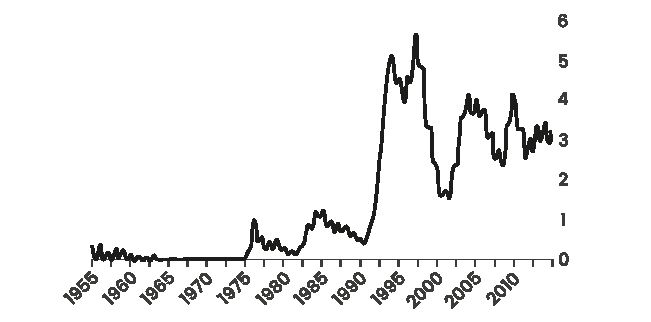
\includegraphics[width=\textwidth]{figures/fig7.pdf}
\caption[Werkloosheidspercentage in Zwitserland]{Werkloosheidspercentage in Zwitserland}
\label{fig7}
\end{figure}

In een vrije markt met gezond geld\index{gezond geld} neemt spaargeld gedurende de tijd in
marktwaarde toe, en hebben individuen de vrijheid om wel of niet te
werken. Ze kunnen elk gewenst loon vragen. Werkgevers hebben ook de
vrijheid om elk gewenst salaris te betalen. In zo'n
wereld waarin spaartegoeden\index{spaartegoeden} in waarde stijgen, is het volkomen rationeel
dat velen ervoor kiezen om geen werk te zoeken. Een werknemer die geen
werk kan vinden tegen een geldend loon, kan simpelweg niemand vinden die
de marginale opbrengst van zijn arbeid hoger waardeert dan de werknemer
zijn persoonlijke waardering van vrije tijd. Het moderne fenomeen van
massale, onvrijwillige werkloosheid is alleen mogelijk wanneer wetten,
regels of beperkingen bestaan die het illegaal en strafbaar maken om
arbeid te verrichten tegen specifieke loonniveaus.

In de context van vrije handel kan er onder mensen die bereid zijn om te
werken geen sprake zijn van werkloosheid, aangezien dat zou betekenen
dat ze recht hebben op een loon dat niemand bereid is hen te betalen. De
werknemer zou altijd werk kunnen vinden door zijn productiviteit te
verhogen of zijn gevraagde loon te verlagen. Gedwongen werkloosheid is
onmogelijk in een vrijemarkteconomie; het is de keuze van de werknemer
om een loon te vragen dat niemand bereid is te betalen, en daardoor is
het hun keuze om werkloos te blijven.

\section{Komt er ooit een einde aan werk?}

Arbeid is als productiemiddel uiterst waardevol, juist omdat het met
vrije tijd concurreert om het meest schaarse productiemiddel, de
menselijke tijd. Naarmate het inkomen en nut dat je door werk krijgt toeneemt, neemt de welvaart van werknemers toe. Dit stelt hen in staat
zich meer vrije tijd te veroorloven, maar het vergroot ook de
vermindering van het nut van hun arbeid en ontmoedigt hen om te werken.
Arbeid zou het enige economische goed of activiteit kunnen zijn waarvan
de geleverde hoeveelheid kan afnemen naarmate de prijs\index{prijs} stijgt. Dit komt
doordat een stijging van de arbeidsprijs leidt tot een toename van de
rijkdom van de werknemer, waardoor hij meer vrije tijd kan kopen en
minder arbeid hoeft te verkopen. De schaarste\index{schaarste} aan tijd betekent dat het
aanbieden van arbeid opportuniteitskosten met zich meebrengt die
toenemen naarmate een persoon meer verdient met werken. Deze dynamiek
heeft velen doen speculeren dat economische vooruitgang op een dag zou
kunnen betekenen dat mensen niet meer hoeven te werken.

Zullen we ooit een punt bereiken waarop we niet meer hoeven te werken?
Dit is een veel voorkomende fantasie onder politici en economen die niet
vertrouwd zijn met de economische manier van denken, zoals John Maynard
Keynes en zijn vele volgelingen. In de jaren `30 speculeerde Keynes dat
de productiviteit zo sterk zou blijven stijgen dat mensen tegen 2030
slechts 15 uur per week zouden moeten werken om te produceren wat ze
nodig hebben. Keynes fantaseerde dat technologische vooruitgang zou
leiden tot technologische werkloosheid, die hij definieerde als
`werkloosheid door onze ontdekking van middelen om sneller op het
gebruik van arbeid te besparen dan het tempo waarin we nieuwe
toepassingen voor arbeid kunnen vinden.'\autocite{43}

`Dit alles betekent op de lange termijn dat de mensheid haar economisch\index{economisch}
probleem oplost', concludeerde Keynes. Hij zag het economisch\index{economisch} vraagstuk
als een wiskundig probleem dat maar éénmaal opgelost hoeft te worden om
definitief opgelost te zijn. Hij ging ervan uit dat het vooral draaide
om het veiligstellen van een bepaalde verzameling goederen en diensten
die nodig zijn voor een gelukkig leven. Wanneer daar eenmaal voor was
gezorgd, zou het economisch\index{economisch} probleem voor eens en altijd zijn opgelost,
waardoor niemand ooit meer economisch\index{economisch} zou hoeven te handelen. In
werkelijkheid is het economisch\index{economisch} vraagstuk een permanent onderdeel van
het menselijk bestaan. We worden voortdurend geconfronteerd met keuzes
tussen schaarse dingen, omdat die schaarste\index{schaarste} voortkomt uit onze beperkte
en extreem kostbare tijd. Zolang mensen leven en moeten beslissen hoe ze
hun tijd willen besteden, zal het economische vraagstuk blijven bestaan
en zullen mensen het proberen op te lossen door te werken. Er kan geen
definitieve oplossing zijn voor het economisch\index{economisch} vraagstuk, alleen de
vervanging van slechte keuzes door betere keuzes.

`Ik concludeer dat, ervan uitgaande dat er geen belangrijke oorlogen en
geen belangrijke bevolkingsgroei zullen zijn, het economisch\index{economisch} probleem
binnen honderd jaar opgelost kan zijn, of op z'n minst
een oplossing in zicht is... Dus voor de eerste keer sinds zijn
schepping zal de mens worden geconfronteerd met zijn echte en permanente
probleem -- hoe hij zijn vrij zijn van dringende economische zorgen moet
gebruiken, hoe hij de vrije tijd, die wetenschap en samengestelde rente\index{rente}
hebben voortgebracht, moet besteden om wijs, aangenaam en goed te
leven.'\autocite{45}

Keynes lijkt zich niet bewust te zijn van het feit dat wat hij voorstelt
als een vervanging voor het economisch\index{economisch} probleem, gewoon het economisch\index{economisch}
probleem zelf is, maar dan toegepast op keuzes die iets anders zijn dan
die hij gewend was te zien in de zeer weinige economische boeken die hij
had gelezen. Het eeuwige en universele economische probleem van de mens
is hoe we onze tijd besteden, omdat tijd schaars is. De simplistische
opvatting van Keynes over de economie maakt het hem onmogelijk te
onderkennen dat het gebruik van tijd een economische keuze is.

Ongeacht hoeveel materiële dingen we hebben, we zullen altijd een keuze
moeten maken in de marge van directe en toekomstige voldoening. We
kunnen altijd huidige voldoening opgeven voor meer toekomstige
voldoening. Er zal nooit volledige voldoening zijn, omdat het menselijk
verstand altijd een betere mogelijkheid zal voorzien en ernaar zal
streven. Het zou voor iemand heel goedkoop zijn om vandaag te leven
volgens de levensstandaard van Keynes' tijd. Toch
kunnen zelfs de armste mensen vandaag de dag veel dingen gebruiken en
bezitten die Keynes nooit heeft kunnen bezitten. En ze blijven verlangen
naar een beter leven, net als de rijkste mensen. Zolang mensen
economisch\index{economisch} handelen, gebruiken ze hun verstand om nieuwe goederen,
diensten en objecten te produceren die anderen wensen.

Keynes baseert zijn fantasierijke visie van de toekomst op een volledig
ongegronde bewering dat er twee soorten behoeften zijn: absolute en
relatieve behoeften. Absolute behoeften, zo stelde Keynes, zijn
behoeften die we voelen `ongeacht de situatie van onze medemensen'.
Daarentegen worden relatieve behoeften alleen gevoeld `als hun
vervulling ons boven onze medemensen uit tilt, ons een gevoel van
superioriteit geeft'.\autocite{46} Keynes stelt dat de vraag naar het voldoen 
van het laatste wellicht onverzadigbaar zou kunnen zijn, maar dat aan de vraag 
naar de vervulling van de eerste klasse van behoeften volledig voldaan zou 
kunnen worden. Keynes dacht dat het economisch\index{economisch} probleem altijd het primaire en
dringendste probleem van het menselijk ras en het hele biologische rijk
is geweest. Het oplossen ervan zou een buitengewoon belangrijke
verandering in de aard van het menselijk leven betekenen. Hij begreep
echter niet dat het economisch\index{economisch} probleem altijd bestaat zolang menselijke
tijd schaars is en mensen keuzes moeten maken. Zelfs als mensen zich in
een denkbeeldige wereld bevonden waarin alles wat ze zich wensen
onmiddellijk wordt gerealiseerd, dan nog zou het economisch\index{economisch} probleem
niet zijn opgelost. De sterfelijkheid van de mensen dwingt hen nog
steeds om economisch\index{economisch} met hun schaarse tijd om te gaan. Het economisch\index{economisch}
probleem wordt elke seconde opgelost wanneer een mens nadenkt over zijn
tijd en een keuze maakt. Maar dan dient zich in de volgende seconde een
nieuw economisch\index{economisch} probleem aan dat dezelfde mens dwingt om opnieuw een
keuze te maken. De enige definitieve oplossing voor het economisch\index{economisch}
probleem is de dood, het moment waarop er geen verdere keuzes meer zijn
over de verdeling van de tijd.

Het is dus onzinnig om je zoals Keynes voor te stellen dat werk
ooit zou kunnen stoppen, of dat de behoefte aan werk ooit zou kunnen
verdwijnen, of dat overvloed een punt zou bereiken waarop arbeid niet
meer nodig is. We handelen voortdurend economisch\index{economisch} en we moeten altijd
keuzes maken tussen alternatieven. Naarmate onze levensstandaard
verbetert, verbeteren onze keuzes, maar het maken van keuzes moet
blijven bestaan, in ieder geval zolang mensen sterfelijk zijn.

\section{Is werk uitbuiting?}

Worden arbeiders uitgebuit door het kapitalisme\index{kapitalisme}? Er zijn miljoenen
pagina's geschreven over het onderwerp van uitbuiting
van arbeiders, voornamelijk gebaseerd op het onsamenhangende gewauwel
van Karl Marx. Marx was een semi-geletterde Duitse zwerver die nooit een
baan had die hem kon onderhouden. Marx leefde van de steun van rijke weldoeners 
terwijl hij orakelde over het herontwerpen van de wereld tot een dystopie, 
geleid door mensen die niet in staat zijn zichzelf te onderhouden door hun eigen arbeid.

Marxistische economische analyse is gebaseerd op de arbeidswaardeleer,
besproken in Hoofdstuk 2. Aangezien alle economische goederen arbeid
vereisen om ze te veranderen in bruikbare economische goederen,
concludeert de marxist ten onrechte dat arbeid economische goederen
waarde geeft en dat de hoeveelheid arbeid die voor de productie\index{productie} van een
goed gebruikt wordt, de waarde ervan bepaalt. Dit betekent dat de waarde
van goederen is gebaseerd op de hoeveelheid arbeid die nodig is voor hun
productie\index{productie}. Door de ongegronde aanname te gebruiken dat economische
waarde puur wordt toegekend aan objecten op basis van de hoeveelheid
arbeid die in hen wordt gestopt, schakelt de marxist automatisch de
waarde van de bijdrage van de kapitalist uit. De arbeiders moeten komen
opdagen en werken, terwijl de kapitalisten, zoals de socialisten
beweren, niets doen. Volgens dit standpunt exploiteert de kapitalist de
arbeider, omdat de arbeider niet de volledige winst ontvangt van het
productieproces\index{productieproces}.

De bewering dat werknemers geen keuze hebben dan voor kapitalisten te werken, is duidelijk incorrect. Werknemers maken immers vrijwillig de keuze om voor deze zogenaamde uitbuiters te werken, een feit dat marxisten vaak negeren. Zolang kapitalisten geen geweld of dreiging met geweld gebruiken om werknemers te dwingen voor hen te werken, is de keuze van werknemers om werk te aanvaarden een indicatie dat zij het zien als de beste manier om hun tijd te besteden. Hoewel buitenstaanders of economen deze situatie misschien betreurenswaardig vinden, kunnen zij kapitalisten niet verwijten dat zij werknemers de beste beschikbare optie bieden in ruil\index{ruil} voor hun tijd. Het is opmerkelijk dat marxisten die kritiek hebben op deze verhoudingen niet in staat zijn om werknemers betere arbeidsmogelijkheden te bieden dan de zogenaamde kapitalistische `uitbuiters'.

Het zien van arbeid als een vorm van uitbuiting toont een diep gebrek aan begrip over de essentie en de waarde van kapitaal\index{kapitaal} voor economische productie\index{productie}. Kapitalisten kiezen ervoor hun consumptie\index{consumptie} uit te stellen om werknemers van kapitaal\index{kapitaal} te voorzien, wat de productiviteit van de werknemers verhoogt. Ze staan voortdurend voor de keuze om consumptie\index{consumptie} uit te stellen ten behoeve van het verschaffen van kapitaal\index{kapitaal} aan werknemers. Immers, kapitalisten hebben de mogelijkheid hun kapitaalgoederen\index{kapitaalgoederen} op ieder moment te liquideren en de opbrengsten te besteden aan consumptie\index{consumptie}. Door de keuze te maken consumptie\index{consumptie} uit te stellen en kapitaal\index{kapitaal} ter beschikking te stellen, maakt de kapitalist het mogelijk voor een werknemer om een hogere productiviteit te bereiken. Dit hogere niveau van productiviteit zorgt ervoor dat de werknemer tevreden is, ook al ontvangt hij slechts een deel van de opbrengst. Het alternatief voor deze zogenaamde kapitalistische uitbuiting is niet dat de werknemer alle inkomsten uit de verkoop van de geproduceerde goederen krijgt; het alternatief zou zijn dat de opbrengsten aanzienlijk lager zijn zonder de inbreng van kapitaal\index{kapitaal}. Een marxist zou kunnen beweren dat een taxichauffeur uitgebuit wordt door de eigenaar van de auto die hij bestuurt, maar dit perspectief miskent wat er zou gebeuren als de chauffeur geen vergoeding zou betalen voor het gebruik van de auto. Zonder een rendement op zijn investering te ontvangen, zou de kapitalist de auto liever als een consumptiegoed\index{consumptiegoed} inzetten of verkopen om de opbrengst te consumeren. Zonder toegang tot de auto zou de chauffeur genoodzaakt zijn mensen op zijn rug te vervoeren, een uiterst inefficiënte en fysiek belastende manier van werken. Het is pas door de zogenaamde 'uitbuiting' door een kapitalist, die hem van kapitaal\index{kapitaal} (de auto) voorziet, dat de arbeid van een chauffeur productief en veilig genoeg wordt om hem een fatsoenlijk leven te bieden.

Het productieproces\index{productieproces} vraagt niet alleen om de tijd van de werknemer, maar ook om de bijdrage van kapitaal\index{kapitaal} door de kapitalist. Dit kapitaal\index{kapitaal} kan alleen verkregen worden door arbeid die al eerder is verricht en kan alleen behouden blijven door consumptie\index{consumptie} gedurende het gehele productieproces\index{productieproces} continu uit te stellen. Zonder compensatie voor de kapitalist voor haar keuze om bevrediging uit te stellen en te investeren, zou er geen kapitaal\index{kapitaal} beschikbaar zijn, wat de productiviteit van de werknemer aanzienlijk zou verminderen. De kapitalist exploiteert de werknemer niet door een deel van zijn productie\index{productie} op te eisen; in plaats daarvan betaalt de werknemer vrijwillig een deel van zijn productie\index{productie} aan de kapitalist, als ruil\index{ruil} voor een veel hoger niveau van productiviteit.

De relatie tussen arbeider en kapitalist is een kenmerk van menselijke
relaties dat in alle menselijke culturen heeft bestaan. Het weerspiegelt
een natuurlijke ruil\index{ruil} tussen een individu dat de capaciteit heeft
om te werken, maar niet de middelen heeft om het noodzakelijke kapitaal\index{kapitaal}
veilig te stellen, en een ander individu dat meer kapitaal\index{kapitaal} heeft dan ze
kan of wil benutten. Het voortbestaan van deze relatie is wat mensen
aanzet tot het vergaren van kapitaal\index{kapitaal}. Het pathologiseren en bestraffen
ervan heeft echter geleid tot een rampzalige economische vernietiging in
samenlevingen.

\chapter{Eigendom}

\begin{blockquotebox}
    Alleen omdat er schaarste\index{schaarste} bestaat, is er een probleem bij het formuleren van morele wetten; want zodra goederen in overvloed (\enquote{vrije} goederen) aanwezig zijn, doet het conflict over het gebruik ervan zich niet voor en is coördinatie overbodig. Hieruit volgt dat een juist begrepen ethiek geformuleerd moet worden als een eigendomstheorie, dat wil zeggen, een theorie over het toekennen van exclusieve controlerechten over schaarse middelen. Dit is de enige manier om anders onvermijdelijke en onoplosbare conflicten te voorkomen.\footnotemark
    \par\raggedleft--- Hans-Hermann Hoppe\index{Hans-Hermann Hoppe}
\end{blockquotebox}
\footautocite{47}


\section{Schaarste en eigendom}

\lettrine{H}oofdstuk 3 behandelde het proces van economisch\index{economisch} handelen als gevolg van de schaarste\index{schaarste} van menselijke tijd. Hoofdstuk 4 onderzocht hoe mensen hun tijd economiseren door een keuze te maken tussen vrije tijd en arbeid, en legde de basisprincipes uit van het productieproces\index{productieproces}. Hoofdstuk 5 onderzoekt het proces van economisch\index{economisch} handelen met goederen en de economische reden voor het ontstaan van eigendom. Na uitleg over de economische betekenis van eigendom, behandelt dit hoofdstuk verschillende soorten eigendom, de toepassing van eigendom op zelfbeschikking en hoe eigendom als instituut helpt in de eeuwige zoektocht om de waarde en hoeveelheid menselijke tijd te vergroten.

Zoals besproken in het eerste hoofdstuk van dit boek, is schaarste\index{schaarste} het startpunt van economie en de oorsprong van al het economisch\index{economisch} handelen. Het is het verschil tussen de gewenste en beschikbare hoeveelheid van een goed dat mensen dwingt om zorgvuldig met dat goed om te gaan, het in optimale conditie te houden om zijn functies te kunnen vervullen, en het te beschermen tegen het feit dat anderen het voor zichzelf kunnen nemen. Schaarste is wat ons dwingt om objecten te waarderen en door ze te waarderen ontwikkelen we er in de loop van de tijd controle over. Schaarste is dan ook de oorsprong van eigendom. Zoals Menger uitlegt:

\begin{blockquotebox}
    Eigendom is net zoals de menselijke economie geen toevallige uitvinding. Het is eerder de enige praktisch mogelijke oplossing voor het probleem dat door de aard der dingen aan ons wordt opgelegd door het verschil tussen de behoeften aan, en de beschikbare hoeveelheden van alle economische goederen.\footnotemark
\end{blockquotebox}
\footautocite{48}


Een goed in eigendom hebben betekent de volledige controle uitoefenen over de diensten die daaruit kunnen voortvloeien. Menger definieert eigendom als \enquote{de totale som van goederen waarover een economisch\index{economisch} handelend individu volledige beschikkingsmacht heeft voor de voldoening van zijn behoeften.}\autocite{49} De wetsgeleerde A. N. Yiannopolous schrijft:

\begin{blockquotebox}
    Eigendom kan worden gedefinieerd als een exclusief recht om de controle uit te oefenen over een economisch\index{economisch} goed...; het is de naam van een concept dat verwijst naar de rechten en verplichtingen, privileges en beperkingen die de relatie van de mens met waardevolle dingen bepalen. Mensen verlangen overal en altijd naar het bezit van dingen die noodzakelijk zijn voor overleving of waardevol zijn volgens culturele normen en die, als gevolg van de vraag naar die zaken, schaars worden. Wetten, die worden afgedwongen door een georganiseerde samenleving, regelen de competitie om deze gewenste dingen en garanderen het genot ervan. Wat gegarandeerd van iemand is, is eigendom. [Eigendomsrechten] verlenen een direct en onmiddellijk gezag over een ding.\footnotemark
    \par\raggedleft--- Hans-Hermann Hoppe\index{Hans-Hermann Hoppe}
\end{blockquotebox}
\footautocite{50}

Eigendom is iets anders dan rijkdom, wat Menger definieert als \enquote{de volledige som van economische goederen die ter beschikking staan van een economisch\index{economisch} handelend individu.} \autocite{51} Iemands eigendom bevat ook alle niet-economische goederen, maar rijkdom verwijst alleen naar economische goederen.

De economische reden voor het hebben van eigendom is duidelijk en eenvoudig. Als het gebruik van een economisch\index{economisch} goed het niet verbruikt en het niet onbruikbaar maakt, kan het opnieuw worden gebruikt voor hetzelfde doel. De gebruiker zou het dan ook vanzelfsprekend het in eigendom willen houden tot hij of zij het weer nodig heeft. Een jager die een speer maakt om een konijn te doden, zal instinctief begrijpen dat de speer opnieuw kan worden gebruikt om een ander konijn te jagen en zal ervoor kiezen de speer in zijn bezit te houden. Heel weinig dieren hebben het instinct om objecten in bezit te nemen en misschien nemen niet-menselijke soorten alleen maar eigendom van hun woonplaatsen, nesten of holen. Door het superieure intellect van de mens kunnen wij op een veel meer verfijnde en complexe manier een bezitsdrang ontwikkelen en blijven dingen voor jaren, decennia en zelfs eeuwen het eigendom van meerdere generaties van dezelfde familie.

Door waardevolle objecten in eigendom te nemen, kunnen mensen de kosten en tijd die nodig zijn om toekomstige taken uit te voeren, verminderen. De eigenaar van duurzame goederen kan haar doel bereiken met minder inspanning en kosten dan iemand die niet hetzelfde eigendom heeft. Het investeren van arbeid in het bouwen van een degelijk huis voor de langere termijn is een effectievere manier om onderdak te regelen dan elke dag een nieuwe provisorische oplossing te zoeken. Het temmen en houden van dieren kan een betrouwbaardere manier zijn om voedsel te verkrijgen, dan elke dag te moeten jagen. Het cultiveren van je eigen bomen en gewassen kan betrouwbaarder en productiever zijn dan het elke dag zoeken naar planten. Dit zijn allemaal methoden waarmee mensen economiseren om hun overlevingskansen te verbeteren en de waarde van hun tijd te verhogen, met andere woorden, de hoeveelheid en de waarde van de tijd die ze op aarde hebben te vergroten.

We kunnen eigendom ook zien als een manier om de tijd die aan arbeid wordt besteed om te zetten in toekomstig nut. Door zijn arbeid te gebruiken om een duurzaam goed te produceren, ziet de mens af van directe voldoening, om zo een goed te maken dat continu nut levert over een toekomstige periode. De meest basale behoeften van de mens kunnen effectiever worden vervuld door te investeren in duurzaam eigendom. Het besteden van arbeid aan het bewerken van een stuk grond geeft een reden om op dat stuk grond te blijven en er blijvend van te profiteren. Het bezit van land maakt een langetermijninvestering en de verhoging van het nut mogelijk, meer dan wanneer het zonder eigenaar bleef, omdat het gebrek aan eigendom investeringen ontmoedigt.

Het belang van eigendom binnen de sociale context is dat het conflicten over schaarse middelen voorkomt. Zoals Stephan Kinsella het verwoordt:

\begin{blockquotebox}
    Er is altijd de mogelijkheid van conflict over betwistbare (schaarse) middelen. Dit zit in de aard van schaarse of concurrerende middelen. Door aan elk goed een eigenaar toe te wijzen, stelt het juridische systeem van eigendomsrechten objectieve, publiekelijk zichtbare of waarneembare grenzen vast waar niet-eigenaars zich aan kunnen houden.\footnotemark
\end{blockquotebox}
\footautocite{52}


\section{Soorten eigendom}

Fysieke goederen kunnen worden geclassificeerd in vier types: bederfelijke goederen, duurzame goederen, kapitaalgoederen\index{kapitaalgoederen} en monetaire goederen. Consumptiegoederen zijn de uiteindelijke doelen van het economisch\index{economisch} handelen, ofwel de goederen die mensen aanschaffen voor eigen gebruik. Duurzame consumptiegoederen\index{consumptiegoed} onderscheiden zich van bederfelijke consumptiegoederen\index{consumptiegoed} doordat ze lange perioden in bezit worden gehouden, omdat hun consumptie\index{consumptie} over een langere duur kan worden uitgespreid. Voorbeelden van duurzame consumptiegoederen\index{consumptiegoed} zijn huizen, auto's, televisies, of wasmachines. Kapitaalgoederen zijn goederen die worden aangekocht vanwege hun vermogen om consumptiegoederen\index{consumptiegoed} te produceren. Monetaire goederen zijn goederen die niet worden bewaard om te consumeren of om consumptiegoederen\index{consumptiegoed} mee te produceren, maar om later te worden ingewisseld voor andere goederen.

In een sociaal systeem dat bevorderlijk is voor individuen die economiseren en zo veel mogelijk conflicten proberen te vermijden, kunnen eigendomsclaims worden vastgesteld op basis van \enquote{het bestaan van een objectieve en intersubjectief verifieerbare link tussen de eigenaar en het geclaimde hulpmiddel}, zoals Hoppe het zegt.\autocite{53} In een vrije markt, of in een sociale orde zonder dwang, zijn er drie manieren voor individuen om legitiem eigendom te verwerven, zoals Rothbard uitlegt:

\begin{enumerate}
\def\labelenumi{\arabic{enumi}.}
\item Het claimen van objecten die nog geen eigenaar hebben
\item Producten die afgeleid zijn van deze objecten
\item Objecten op vrijwillige basis verkregen van rechtmatige eigenaren, \\hetzij door (ruil\index{ruil})handel, hetzij als een geschenk.
\end{enumerate}

\section{Zelfbeschikking}

Omdat mensen schaars zijn, en hun tijd ook, is het alleen maar vanzelfsprekend dat dezelfde implicaties van schaarste\index{schaarste} voor economische goederen ook op mensen van toepassing zijn. Eigendom is volgens Menger de \enquote{enige praktische oplossing}. Hoewel het idee van eigendom van mensen schokkend en moreel verkeerd klinkt, is het in economische termen onvermijdelijk. Aangezien mensen en hun tijd schaars zijn, moeten de beslissingen over hoe een mens zich gedraagt en wat hij met zijn tijd doet door iemand worden genomen. Dat is de essentie van eigendom. De persoon die beslist wat er met het lichaam en de tijd van een persoon moet gebeuren, bezit \emph{de facto} deze economisch\index{economisch} gezien. De kwalificatie \enquote{afschuwelijk} is alleen van toepassing en gepast wanneer de vraag naar eigendom in het voordeel van iemand anders dan de persoon zelf wordt beantwoord.

Er zijn slechts drie mogelijke manieren om het eigendom van mensen te regelen:

\begin{enumerate}
\def\labelenumi{\arabic{enumi}.}
\item Via zelfbeschikking, waarbij een persoon zichzelf volledig bezit en anderen geen eigendomsrechten kunnen claimen over zijn lichaam en tijd.
\item Gemeenschappelijk eigendom, waarbij alle leden van de samenleving gezamenlijk al hun lichamen bezitten en gezamenlijk beslissen wat elk lichaam doet.
\item Slavernij, waarin een persoon het eigendom is van iemand anders en zijn eigenaren bepalen wat ze kunnen doen met het lichaam en de tijd van de slaaf. Dit varieert van het toewijzen van zijn tijd aan taken tot het toebrengen van lichamelijke schade. De rechten van slaveneigenaren gaan zelfs zo ver dat ze de slaaf mogen vermoorden. In een sociale orde met slavernij hebben sommige mensen eigendomsrecht over zowel zichzelf als anderen, terwijl anderen geen recht van eigendom hebben over zichzelf of anderen.
\end{enumerate}


De tweede optie is praktisch niet werkbaar buiten de omvang van een handjevol mensen die elkaar goed kennen, en zelfs dan zou het niet gemakkelijk zijn. Mensen zouden het erg moeilijk vinden om alle kennis te vergaren om te beslissen wat anderen met hun leven en tijd zouden moeten doen. De problemen om een mechanisme te bedenken voor informatieoverdracht, besluitvorming en uitvoering in een grootschalig sociaal systeem zijn praktisch onoverkomelijk.

De derde optie faalt op het gebied van consistentie, ethiek en al de gevolgen. Wat voor ethische basis kan er zijn om te rechtvaardigen waarom sommige mensen van zichzelf zijn, terwijl anderen in eigendom zijn van anderen? Er kan geen logisch en ethisch samenhangende manier zijn om dit drastisch verschil in toewijzing van eigendomsrechten te rechtvaardigen. Verder is dit verschil waarschijnlijk een recept voor conflicten. Het individu dat geen zelfeigendomsrechten heeft, zal proberen deze te verkrijgen en kan zich gerechtvaardigd voelen in het gebruik van geweld tegen degenen die hem bezitten. Overal waar slavernij als systeem heeft bestaan, heeft het geleid tot conflict.

Persoonlijke zelfbeschikking is de enige logische en ethisch consistente oplossing voor het probleem van menselijk eigendom, en het is de enige die waarschijnlijk zal leiden tot vreedzame samenwerking in plaats van gewelddadig conflict. Zelfbeschikking betekent dat een individu volledige aanspraak heeft op zijn eigen lichaam en tijd. Wanneer we het principe van zelfbeschikking accepteren, ontstaat er een coherent kader voor het begrijpen van rechten, rechtvaardigheid en non-agressie. Dit principe strekt zich uit tot wat een mens kan produceren als gevolg van deze keuzes, ofwel eigendom. Je kunt agressie zien als het gebruik of de dreiging van geweld om het lichaam of de tijd van een ander persoon te beheersen, en elke fysieke agressie tegen een individu zou een schending zijn van zijn recht op zelfbeschikking.

Als we eigendomsrechten begrijpen als de enige werkende oplossing voor economische schaarste\index{schaarste} en als we vrede en beschaving\index{beschaving} waarderen, is het moeilijk om tegen zelfbeschikking en het systeem van eigendomsrechten te argumenteren. Elk dergelijk argument kan gezien worden als doorzichtig egoïstische hypocrisie. In plaats van een intelligent argument dat voortkomt uit het menselijk verstand, is dit argument niets meer dan een oproep om terug te keren naar de zeden van dieren die volledig door hun instincten worden beheerst, en niet in staat zijn om hun verstand te gebruiken. Argumenteren tegen zelfbeschikking is feitelijk argumenteren tegen je eigen persoonlijke identiteit, omdat het duidelijk maakt dat je geen respect hebt voor eigendomsrechten en geen deel kunt zijn van een beschaafde sociale orde. Het is een pleidooi om als een dier beschouwd te worden. Hoewel economische theorie geen politieke ideologie voorschrijft, zal begrip van economische schaarste\index{schaarste} en een waardering van vrede en beschaving\index{beschaving} een persoon ertoe aanzetten een libertarische kijk aan te nemen. Voor zelfbeschikking bestaan geen alternatieven die niet tot conflict leiden en geen vijandigheid en wrok tussen individuen en groepen creëren.

Hoewel de meeste ideologieën niet expliciet voor slavernij zullen pleiten, volgen alleen libertariërs deze norm strikt tot in al zijn logische consequenties. Alle andere ideologieën geloven in minimaal een bepaalde vorm van slavernij, in de vorm van een legitieme aanspraak van anderen op iemands lichaam of tijd. Voorstanders van belasting, dienstplicht, drugsverboden of medische mandaten vinden het misschien niet leuk om zichzelf te zien als voorstanders van slavernij, maar ze geven een gedeeltelijk eigendomsrecht over iemands lichaam in handen van de staat. Ze doen dit omdat ze de staat steunen als ze haar burgers als eigendom behandelt. Dit gebeurt wanneer de staat hun inkomen met geweld afneemt, ze in de gevangenis opsluit voor het consumeren van drugs, of hen uitsluit van werk voor het niet gebruiken van door de staat verplichte farmaceutische producten.\autocite{54}

\section{Belang van eigendomsrechten}

Door het concept eigendom te begrijpen, kan een individu beter en effectiever economiseren, en de productiviteit en waarde van zijn tijd verhogen. Door zijn arbeid te investeren in de productie\index{productie} van duurzame goederen, kan een mens langer van hun diensten profiteren. Dit verlaagt zijn tijdsvoorkeur\index{tijdsvoorkeur} en hij leert meer prioriteit te geven aan de toekomst.

Wanneer het accepteren van eigendomsrechten de geldende norm wordt in een samenleving, zijn individuen in staat om in kapitaalgoederen\index{kapitaalgoederen} te investeren om met anderen te handelen. Hun productiviteit neemt verder toe en de economische marktorde ontwikkelt zich. Dit wordt besproken in de volgende hoofdstukken. Eigendomsrechten kunnen worden begrepen als het sociale mechanisme dat mensen in staat stelt om hun eigendom te behouden in de nabijheid van anderen die het misschien ook willen bezitten. Zoals Mises het verwoordde, \enquote{privaat eigendom van de productiemiddelen is het fundamentele instituut van de markteconomie. Het is de instelling wiens aanwezigheid de markteconomie kenmerkt. Waar het afwezig is, is er geen sprake van een markteconomie.}\autocite{55}

De markteconomie en de beschaving\index{beschaving} zelf zijn gebaseerd op het respect voor eigendomsrechten. Het is alleen bij veilige eigendomsrechten dat mensen een hoeveelheid kapitaal\index{kapitaal} kunnen vergaren die significant groter is dan wat ze bij zich kunnen dragen voor hun eerste levensbehoeften. Een samenleving waarin eigendomsrechten niet worden gerespecteerd is er een waarin veel conflicten zijn. In zo'n maatschappij kunnen individuen zich niet veroorloven om hun kostbare arbeid in de toekomst te investeren, omdat al het eigendom dat deze waarde kan opslaan, riskant is om te bezitten. Een beschaafde samenleving is alleen mogelijk wanneer het recht op eigendom van jezelf en objecten in brede kring wordt gerespecteerd. Mensen kunnen dan verwachten hun eigendom zeker te stellen voor de toekomst.

In de context van een markteconomie legt Mises op prachtige wijze uit hoe het instituut van privaat eigendom zorgt voor een verantwoord beheer van middelen:

\begin{blockquotebox}
    De betekenis van privaat eigendom in de marktsamenleving is radicaal anders dan onder een systeem van autarkie van elk huishouden. In een situatie waarin elk huishouden economisch\index{economisch} zelfvoorzienend is, dienen de productiemiddelen van het private eigendom uitsluitend de eigenaar. Alleen dit huishouden plukt de vruchten van het gebruik. In de marktsamenleving kunnen de eigenaren van kapitaal\index{kapitaal} en land alleen genieten van hun eigendom door het te gebruiken om aan de behoeften van anderen te voldoen. Ze moeten in dienst zijn van de consumenten om enig voordeel te hebben van wat van hen is. Het feit dat ze productiemiddelen bezitten, dwingt hen zich te onderwerpen aan de wensen van het publiek. Eigendom is alleen een voordeel voor degenen die weten hoe ze het op de best mogelijke manier kunnen gebruiken ten behoeve van de consumenten. Het is een sociale functie.\footnotemark
\end{blockquotebox}
\footautocite{56}

De afwezigheid van privaat eigendomsrecht leidt tot conflicten tussen mensen, evenals tot de teloorgang van economische goederen en natuurlijke hulpmiddelen. Wanneer economische goederen geen duidelijke eigendomsrechten hebben, zullen de individuen die ze op enig moment gebruiken en beheren, dit doen zonder de verwachting ze in de toekomst te kunnen gebruiken. Dit leidt ertoe dat ze de toekomstige staat van deze middelen niet als prioriteit zien. Deze sterke onderwaardering van de toekomst is een kenmerkend aspect van het gebruik van goederen zonder een duidelijke eigenaar. Privaat eigendom motiveert eigenaars om zich te bekommeren om de staat van hun eigendom over de lange termijn.


Zoals Mises uitlegt:

\begin{blockquotebox}
    Als land in niemands bezit is, terwijl het formeel wettelijk als publiek eigendom kan worden beschouwd, wordt het gebruikt zonder enige aandacht voor de resulterende nadelen. Personen die in staat zijn om de opbrengsten voor zichzelf toe te eigenen -- het hout en wild uit de bossen, vis uit wateren en minerale afzettingen uit de bodem -- maken zich niet druk over de effecten van hun exploitatiemethoden op langere termijn. Erosie van de bodem, uitputting van eindige bronnen en andere schadelijke effecten op het toekomstig gebruik worden door hen gezien als externe kosten die geen deel uitmaken van hun berekening van input en output. Ze kappen bomen zonder nieuwe scheuten of herbebossing te overwegen. Bij jagen en vissen schrikken ze niet terug voor methoden die herbevolking van de jacht- en visgronden onmogelijk maken. In de vroege dagen van de menselijke beschaving\index{beschaving}, toen er nog volop grond van goede kwaliteit beschikbaar was, zagen mensen dergelijke roofzuchtige methoden niet als een probleem. Toen de effecten merkbaar werden in een afname van de netto-opbrengsten, verliet de boer zijn boerderij en verhuisde hij naar een andere plek. Pas als een land dichter bevolkt raakte en er geen ongebruikt land van topkwaliteit meer beschikbaar was, begonnen mensen dergelijke roofzuchtige methoden als verspilling te beschouwen. Op dat moment consolideerden ze het instituut van privaat eigendom van land. Ze begonnen met landbouwgrond en stapten vervolgens over op weiden, bossen en visgebieden.\footnotemark
\end{blockquotebox}
\footautocite{57}

\hypertarget{kapitaal}{%
\chapter{Kapitaal}\label{kapitaal}}
\vspace{-1em}
\begin{blockquotebox}
    Overal waar we naar beschavingen kijken, treffen we een systeem aan dat op grote schaal in de toekomstige menselijke behoeften voorziet. Terwijl we nog onze winterkleding dragen om ons tegen de kou te beschermen, is de lente-collectie al onderweg naar de winkels. In de fabrieken worden ondertussen lichte stoffen geweven voor de kleding die we volgende zomer zullen dragen, en worden garens gesponnen voor de winterkleding van het jaar daarop. Wanneer we ziek worden, is de hulp van een arts noodzakelijk. Bij juridische conflicten is het advies van een advocaat onmisbaar. In dergelijke situaties zou het veel te laat zijn om op dat moment pas te beginnen met het verwerven van de benodigde medische of juridische kennis en vaardigheden, of om te proberen de gespecialiseerde opleiding van anderen te organiseren, zelfs als men over de benodigde middelen zou beschikken. In ontwikkelde landen worden de behoeften van de samenleving aan dergelijke diensten op tijd ingevuld door ervaren en deskundige professionals, die zich jaren van tevoren al op hun vakgebied hebben voorbereid en sindsdien uitgebreide praktijkervaring hebben opgedaan. Terwijl we zo profiteren van de vooruitziendheid uit het verleden, worden velen op onze universiteiten opgeleid om in de toekomst aan de behoeften van de samenleving te voldoen.\footnotemark
    \par\raggedleft--- Carl Menger\index{Carl Menger}
\end{blockquotebox}
\footautocite{58}


\lettrine{I}n het vorige hoofdstuk bespraken we het begrip eigendom in economische termen en de ontwikkeling van dit menselijke hulpmiddel in de loop van de tijd. De economische wetenschap maakt binnen alle vormen van eigendom een onderscheid tussen consumptiegoederen\index{consumptiegoed}, die eigendom zijn voor het nut dat ze hen bieden, en kapitaalgoederen\index{kapitaalgoederen}, die we bezitten omdat ze gebruikt kunnen worden om nuttige consumptiegoederen\index{consumptiegoed} te produceren. Kapitaalgoederen, ook goederen van hogere orde genoemd, zijn alle goederen die niet geconsumeerd worden, maar die worden gebruikt voor de productie\index{productie} van consumptiegoederen\index{consumptiegoed} of goederen van een lagere orde. Wat van een goed een consumptiegoed\index{consumptiegoed} of kapitaalgoed\index{kapitaalgoederen} maakt, is niet inherent aan het goed zelf, maar hangt af van hoe het goed gebruikt wordt door de persoon die het bezit. Hetzelfde goed kan gebruikt worden als kapitaalgoed\index{kapitaalgoederen} of als consumptiegoed\index{consumptiegoed}, afhankelijk van de context. Een computer die gebruikt wordt om films te kijken en op het web te surfen is een consumptiegoed\index{consumptiegoed}, maar dezelfde computer die gebruikt wordt om een boek te schrijven is een kapitaalgoed\index{kapitaalgoederen}. Een auto kan een kapitaalgoed\index{kapitaalgoederen} zijn als hij als taxi gebruikt wordt, maar een consumptiegoed\index{consumptiegoed} als hij puur voor recreatieve reizen gebruikt wordt. Maïskorrels kunnen een consumptiegoed\index{consumptiegoed} zijn als ze opgegeten worden, maar een kapitaalgoed\index{kapitaalgoederen} als ze geplant worden om meer maïs te verbouwen.

Dit hoofdstuk bespreekt het concept van kapitaal\index{kapitaal} op een abstracte manier. Na het introduceren van geld en de uitgebreide marktorde in de komende hoofdstukken, zal Hoofdstuk 12 kapitaal\index{kapitaal} behandelen in de context van een moderne monetaire economische orde. Deel IV van het boek zal de problemen bespreken van centrale planning op de kapitaalmarkten.

\hypertarget{verlenging-van-het-productieproces}{%
\section{Verlenging van het productieproces}\label{verlenging-van-het-productieproces}}

De invoering van kapitaal\index{kapitaal} in economische productie\index{productie} maakt een verlenging van de productieperiode noodzakelijk. Zonder kapitaalgoederen\index{kapitaalgoederen} houdt de mens zich rechtstreeks bezig met de productie\index{productie} van het uiteindelijke consumptiegoed\index{consumptiegoed}, maar wanneer een kapitaalgoed\index{kapitaalgoederen} gebruikt wordt, moet de mens eerst het kapitaalgoed\index{kapitaalgoederen} produceren en het dan gebruiken om het consumptiegoed\index{consumptiegoed} te produceren. Door een tussenstadium van kapitaalproductie toe te voegen, wordt het productieproces\index{productieproces} van begin tot eind langer.

Dit lijkt in eerste instantie misschien niet intuïtief. Waarom zouden mensen zich immers bezig houden met langere productieprocessen? Tijdsvoorkeur is, zoals besproken in Hoofdstuk 3, altijd positief; mensen hebben eenzelfde goed liever vroeger dan later. Waarom uren besteden aan het bouwen van een hengel om een vis te vangen, als je direct met je handen vis kunt vangen in minder tijd? Het antwoord ligt in de productiviteit van de hengel. Hoewel het produceren van de hengel tijd kost, stelt het de visser hopelijk in staat om een grotere hoeveelheid vis met een gelijke inspanning te vangen vanaf het moment dat de hengel af is. Hoewel de onmiddellijke investering in het maken van een hengel de vangst van de vis vertraagt, maakt de toename in productiviteit zijn lange-termijn opbrengst waardevoller dan de kleinere opbrengst van het vissen met je handen, die sneller wordt gerealiseerd. Het succes van deze investering is niet gegarandeerd, maar de mogelijke extra beloning is de enige motivatie om kapitaal\index{kapitaal} te accumuleren, het productieproces\index{productieproces} te verlengen en de voldoening van behoeften uit te stellen.\autocite{59a, 59b}

Als iemand ervoor zou kiezen om vis met zijn handen te vangen, dan zou de productieperiode starten op het moment dat hij richting de zee gaat om de vis te vangen tot het moment dat hij deze vangt. Laten we aannemen dat dit proces twee uur duurt. Er is geen snellere en directere manier om vis te vangen, maar er zijn productievere manieren, die weliswaar langere productieprocessen hebben. Als de man zich bezig zou houden met het produceren van een visspeer, dan zou de tijd om een geschikte tak te vinden, deze scherp te maken en leren te gebruiken het gehele productieproces\index{productieproces} verlengen. We kunnen wel aannemen dat de tijd vanaf het begin van de zoektocht naar de stok tot het vangen van de vis vier uur zou zijn in plaats van twee. De speer van de visser blijft echter functioneren, en het vangen van de volgende vis zou veel minder tijd in beslag nemen dan de twee uur die het de man gemiddeld vroeger zonder de speer kostte. Het gehele productieproces\index{productieproces} zou langer worden, maar zodra het kapitaal\index{kapitaal} eenmaal geproduceerd is, zou de marginale tijd die nodig is om een extra eenheid te produceren korter worden. Naarmate het proces van kapitaalaccumulatie in de visserij intensiever wordt, wordt het productieproces\index{productieproces} almaar langer: De visser bouwt een kleine boot, wat een volledige productieweek vereist voor hij er een enkele vis mee kan vangen, maar eens hij ermee kan beginnen te vissen, verhoogt het de marginale productiviteit van de visser aanzienlijk. Naarmate de kapitaalaccumulatie zich voortzet, zou de visser een grote boot kunnen bouwen die een volledig productiejaar vereist voor hij een enkele vis oplevert.


\hypertarget{sparen}{%
\section{Sparen}\label{sparen}}

\begin{blockquotebox}
    De onmisbare voorwaarde voor elke verlenging van het productieproces\index{productieproces} is sparen, ofwel, een overproductie ten opzichte van het huidige verbruik. Sparen is de eerste stap op weg naar verbetering van het materiële welzijn en naar elke verdere vooruitgang op dit pad.\footnotemark
    \par\raggedleft--- Ludwig von Mises\index{Ludwig von Mises}

\end{blockquotebox} 
\footautocite{60}

Het verlengen van de productietijd kan niet plaatsvinden zonder eerst de consumptiegoederen\index{consumptiegoed} te leveren die nodig zijn om de producenten tijdens het productieproces\index{productieproces} in stand te houden. Voorzieningen voor de toekomst treffen maakt het mogelijk om productieprocessen te starten die langer en productiever zijn. Maar de mens kan alleen middelen sparen voor de toekomst als hij in staat is om aan zijn huidige behoeften te voldoen. De boer moet genoeg graan produceren om zichzelf te voeden voordat hij graan kan zaaien, en elk graan dat hij zaait, is graan dat hij dit jaar niet kan consumeren. Als de visser een dag gaat besteden aan het bouwen van een hengel, moet hij eerst al voor deze dag hebben gezorgd vanuit zijn productie\index{productie} van de vorige dag door het uitstellen van een deel van de mogelijke consumptie\index{consumptie} tijdens deze vorige dag. Het is onmogelijk om een hengel te bouwen zonder vrije tijd op te geven, dat een positief nut heeft, of arbeid waarmee consumptiegoederen\index{consumptiegoed} met een positief nut worden geproduceerd. Sparen is de moeder van kapitaal\index{kapitaal}; alleen door consumptie\index{consumptie} uit te stellen kunnen kapitaalgoederen\index{kapitaalgoederen} bestaan.

Hetzelfde geldt voor de langste en meest ingewikkelde productieprocessen, zoals het maken van een vliegtuig. Vandaag zijn er ingenieurs actief die de volgende reeks vliegtuigen voor Boeing ontwerpen, een proces dat waarschijnlijk meer dan een decennium aan ontwerpen, productie\index{productie} en testen zal vereisen voordat ze verkocht kunnen worden om inkomsten voor het bedrijf\index{bedrijf} te genereren. De vliegtuigbouwer heeft kapitaal\index{kapitaal} nodig om in het levensonderhoud van deze arbeiders te voorzien voordat het productieproces\index{productieproces} voltooid is en het bedrijf\index{bedrijf} inkomsten kan genereren uit de verkoop van de vliegtuigen, alsook voor de compensatie van de eigenaren van het kapitaal\index{kapitaal} dat gebruikt wordt in het productieproces\index{productieproces}. Tijdsvoorkeur is positief, en eigenaren van kapitaal\index{kapitaal} en arbeiders moeten consumeren tijdens het productieproces\index{productieproces} om te overleven en stellen hiervoor hun kapitaal\index{kapitaal} of arbeid ter beschikking. Zelfs als Boeing op de een of andere manier in staat zou zijn om alle kapitaalgoederen\index{kapitaalgoederen} en arbeid te verkrijgen door aan de arbeiders en verkopers van apparatuur te beloven te betalen wanneer de vliegtuigen voltooid waren, dan zou de productie\index{productie} gefinancierd zijn door de arbeiders en verkopers van machines, die voldoening hadden moeten uitstellen om te kunnen produceren.

\textbf{Om het productieproces\index{productieproces} te verlengen, moet iemand ergens het verbruik van middelen opgeven om deze aan de producenten te geven}. In de eenvoudige visserseconomie maakte de visser zelf de opoffering door wat voedsel van de vorige dag te bewaren voor de erop volgende dag, zodat hij tijd kon besteden aan het maken van een hengel. In een moderne kapitalistische economie wordt de opoffering gemaakt door investeerders die consumptie\index{consumptie} opgeven om financiering te bieden aan ondernemers. De ondernemers vergoeden de werknemers en de eigenaren van het kapitaal\index{kapitaal} voor het leveren van hun arbeid en kapitaal\index{kapitaal} voor het productieproces\index{productieproces}, waarvan de opbrengst in de toekomst gerealiseerd zal worden. Een langer productieproces\index{productieproces} vereist niet alleen meer uitgestelde voldoening, maar ook meer cognitieve vaardigheden en kan meer risico\index{risico}\textquotesingle s met zich meebrengen. Zonder een ondernemer die een langere structuur beoogt en een investeerder die huidige voldoening opoffert voor de kans op een groter toekomstig rendement, kunnen de benodigde kapitaal\index{kapitaal}- en arbeidsmiddelen voor het productieproces\index{productieproces} niet worden aangeschaft. Elk proces dat de productie\index{productie} verlengt, is alleen mogelijk door de opoffering en de uitgestelde voldoening van kapitalisten. Het is het waard om dit schijnbaar vanzelfsprekende punt opnieuw te benadrukken, omdat een aanzienlijk deel van de economische problemen in de wereld worden veroorzaakt door dwazen die met de illusie leven dat ze een uitzondering op deze noodzakelijkheid hebben gevonden.

\hypertarget{hogere-productiviteit}{%
\section{Hogere productiviteit}\label{hogere-productiviteit}}

Ludwig von Mises\index{Ludwig von Mises} beschreef kapitaalgoederen\index{kapitaalgoederen} als ``opgeslagen arbeid, natuur en tijd''.\autocite{61} Hij maakte een onderscheid tussen kapitaal\index{kapitaal} en onafhankelijke productiefactoren, natuurlijke materiële grondstoffen, en arbeid. Dit mentale kader is heel nuttig voor het begrijpen van de economische functie en het belang van kapitaal\index{kapitaal}. Mensen zijn in staat om de door de natuur gegeven grondstoffen en hulpmiddelen te combineren met hun arbeid, en na verloop van tijd kapitaalgoederen\index{kapitaalgoederen} als eindproduct te produceren. De tijd, arbeid en hulpmiddelen die benodigd waren voor de productie\index{productie} van het kapitaalgoed\index{kapitaalgoederen}, resulteren vervolgens in een hogere productiviteit.

Produceren met behulp van kapitaalgoederen\index{kapitaalgoederen} kan gezien worden als produceren met behulp van de arbeid, natuur en tijd die in de vervaardiging van het kapitaalgoed\index{kapitaalgoederen} zijn gestoken. Dit leidt tot een toename in productiviteit, waardoor de productie\index{productie} van een eenheid van het eindproduct minder tijd kost dan zonder kapitaal\index{kapitaal}. Men besteedt tijd aan langere productieprocessen om hogere opbrengsten per tijdseenheid te kunnen behalen, wat van kapitaal\index{kapitaal} een andere manier maakt om menselijke tijd te besparen. Zoals Mises uitlegt: ``Het verschil tussen productie\index{productie} zonder de hulp van kapitaalgoederen\index{kapitaalgoederen} en die met behulp van kapitaalgoederen\index{kapitaalgoederen} zit in tijd... Degene die produceert met behulp van kapitaalgoederen\index{kapitaalgoederen} geniet een groot voordeel ten opzichte van de man die begint zonder kapitaalgoederen\index{kapitaalgoederen}; hij is qua tijd dichter bij het uiteindelijke doel van zijn streven.'' \autocite{62}

Het is belangrijk om de langere periode van het gehele productieproces\index{productieproces} niet te verwarren met de kortere productietijd van het eindproduct. Kapitaal opbouwen leidt tot een toename van de totale tijd die nodig is om goederen te produceren wanneer de goederen van hogere orde die in het proces gaan worden meegerekend. Het leidt echter ook tot een afname van de productietijd van elke marginale eenheid. Kapitaalgoederen maken niet alleen een hogere productiviteit mogelijk, maar ook de productie\index{productie} van goederen die zonder kapitaal\index{kapitaal} volstrekt onmogelijk waren. De visser die overstapt van vissen met de hand naar het gebruik van een vishengel of vissersboot zal niet alleen een hogere productie\index{productie} hebben, maar hij zal ook in staat zijn om vissen te vangen die buiten zijn bereik lagen voordat hij het kapitaal\index{kapitaal} had. Zonder kapitaalopbouw zouden de meeste producten die we als vanzelfsprekend aannemen in de moderne wereld niet mogelijk zijn, omdat er geen manier is om ze met onze blote handen te produceren.

Kapitaalgoederen worden gebouwd en aangeschaft om de productiviteit van arbeid te verhogen, en daarbij maken ze het hele productieproces\index{productieproces} onvermijdelijk langer. Kapitaal is het verschil tussen het vissen met je blote handen en vissen met een hengel, met een kleine vissersboot of met de \emph{Annelies Ilena}, de grootste open trawler ter wereld. Een dag vissen met je handen levert als je geluk hebt een paar vissen op. Met een hengel zou je op een dag ongeveer een dozijn vissen kunnen vangen en met een vissersboot en een net enkele honderden. Aan de andere kant zou je met ongeveer 70 bemanningsleden van de Annelies Ilena elke dag samen ongeveer 350 ton vis produceren, of ongeveer 5 ton vis per werknemer per dag. Dezelfde mens, die hetzelfde aantal uren besteedt tijdens dezelfde dag, zou één vis of 5 ton vis kunnen vangen, enkel afhankelijk van het kapitaal\index{kapitaal} dat hij ervoor kan inzetten.

\begin{figure}[]
    \centering
    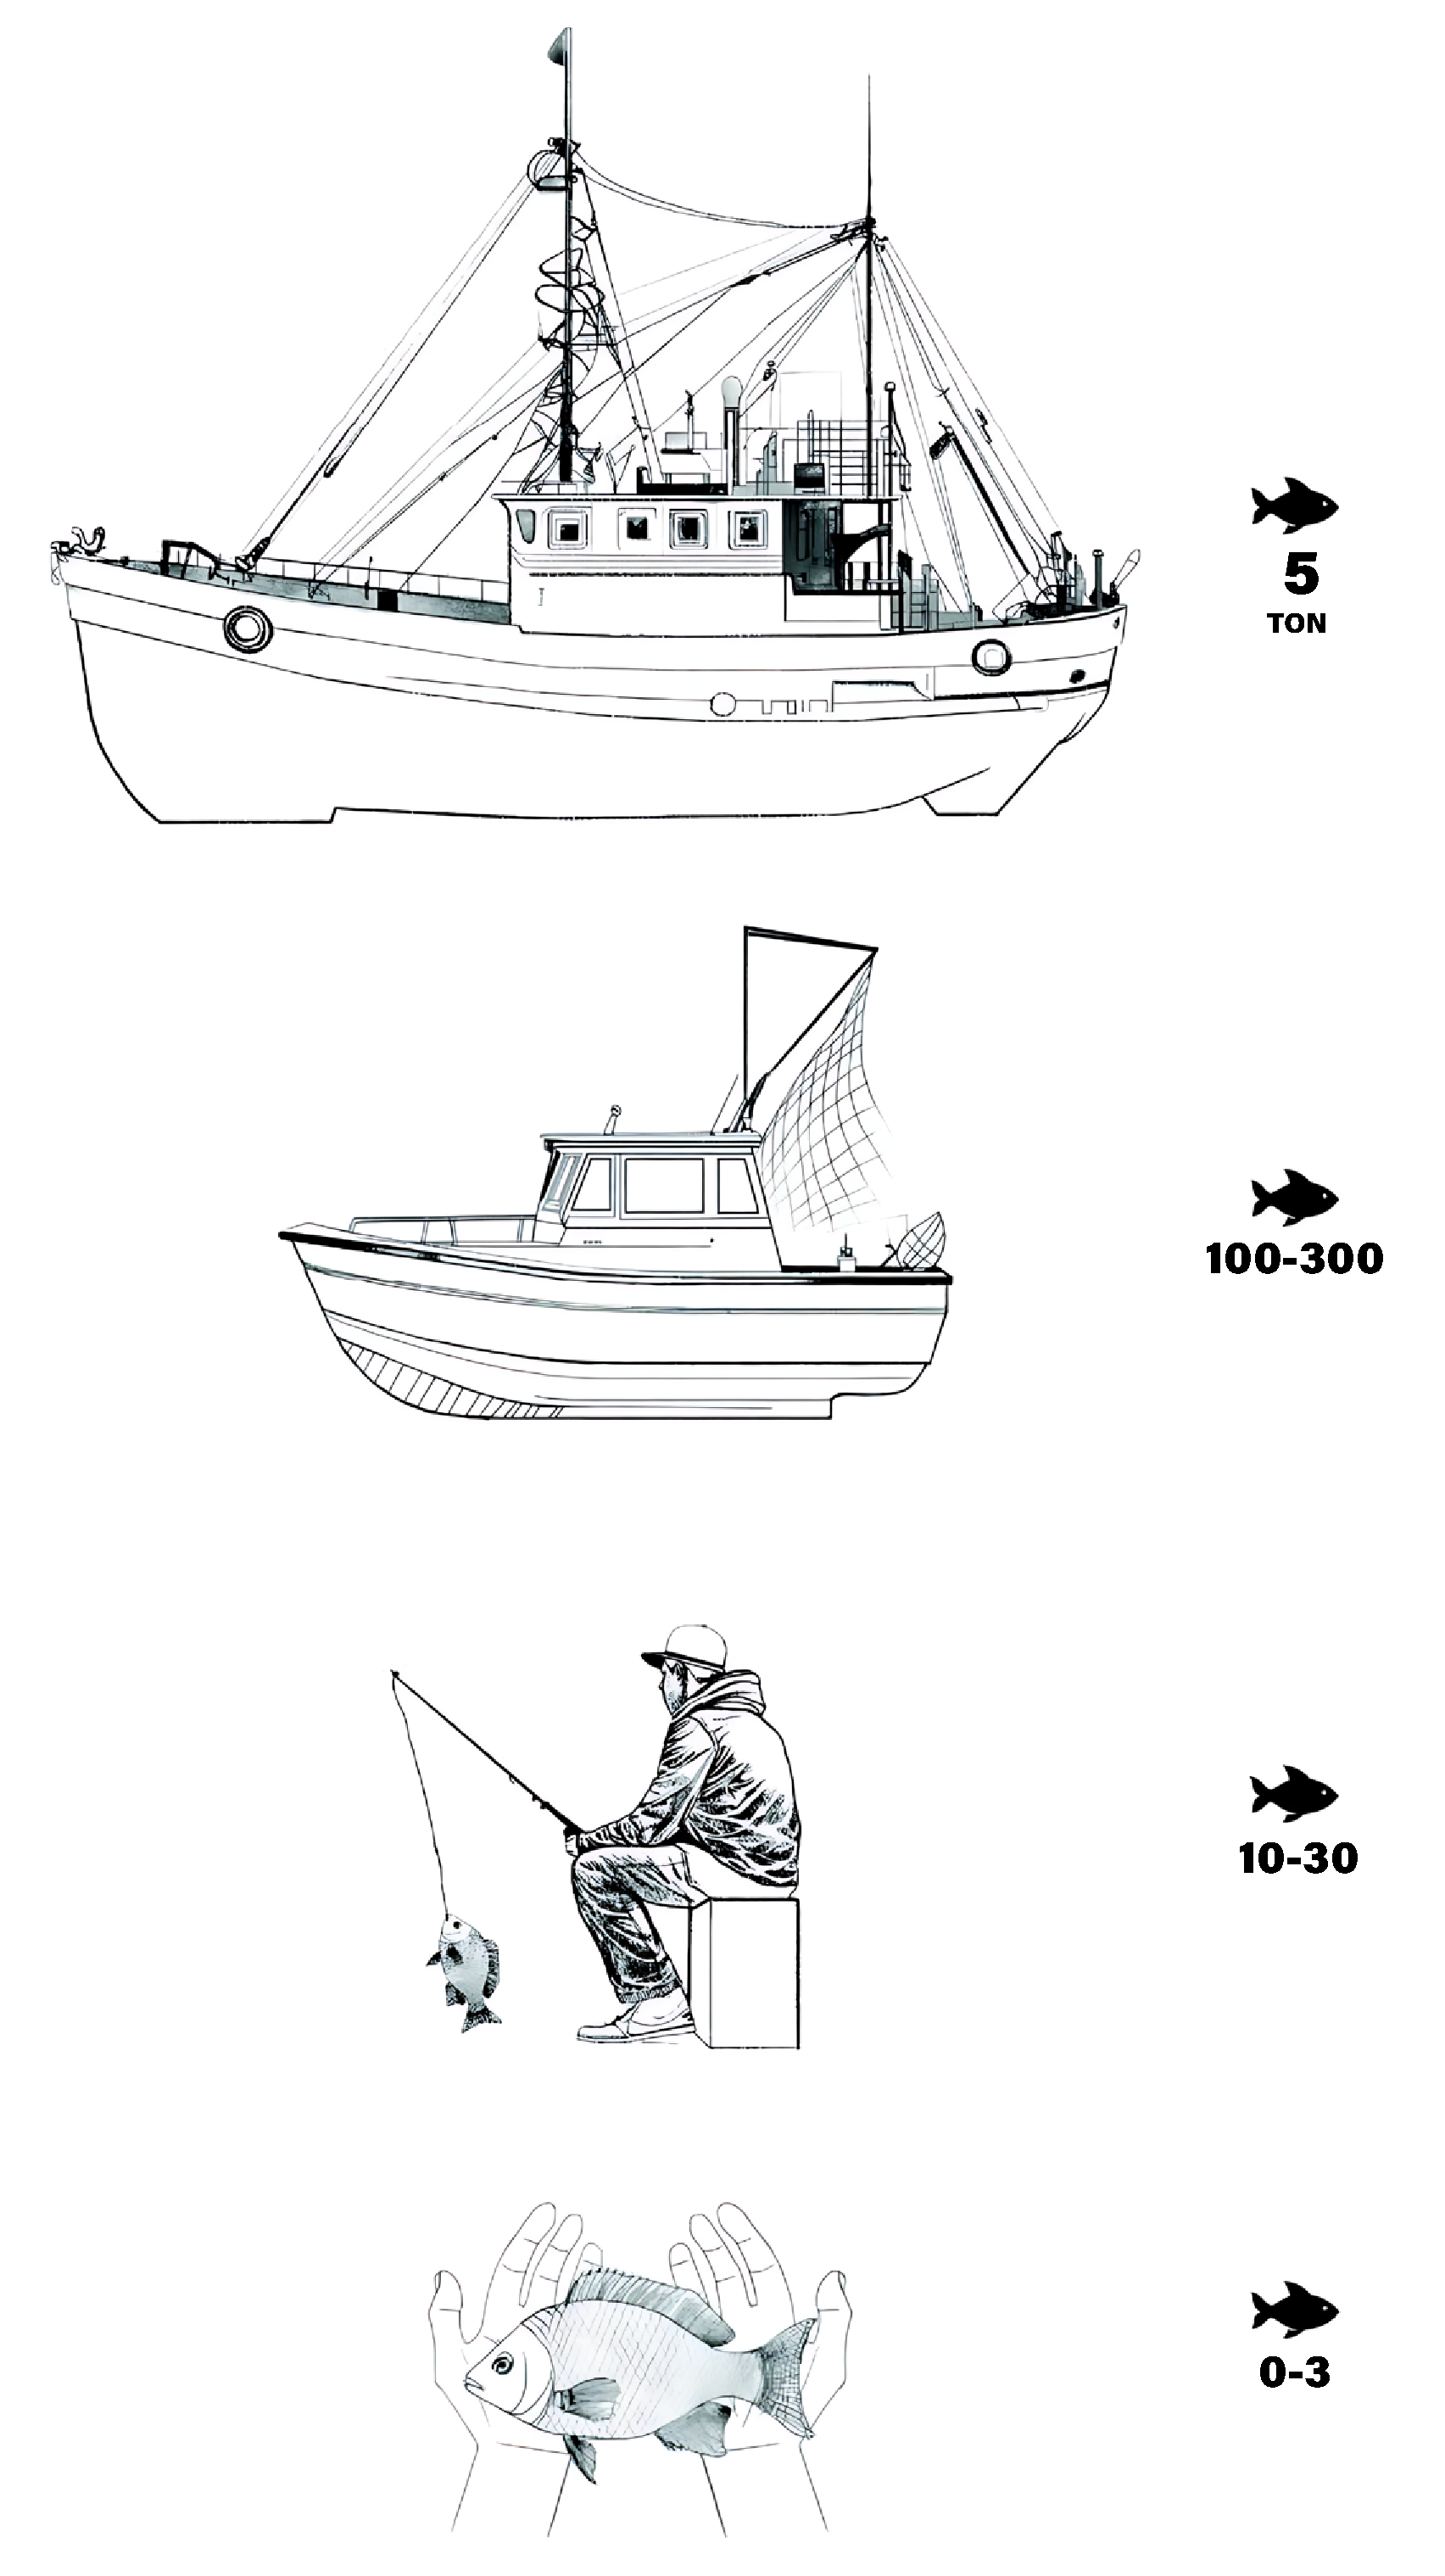
\includegraphics[width=0.8\textwidth]{figures/fig8.pdf}
    \caption[Productiviteit en kapitaal\index{kapitaal}]{Productiviteit en kapitaal\index{kapitaal}}
    \label{fig8}
\end{figure}

Deze toename in productiviteit is uiteindelijk wat het verschil in levensstandaard uitmaakt tussen mensen die met grote hoeveelheden kapitaal\index{kapitaal} kunnen werken en mensen die dat niet kunnen, tussen mensen die met hun blote handen vissen en mensen die met de Annelies Ilena vissen, tussen landen met een grote hoeveelheid industrieel kapitaal\index{kapitaal} en landen zonder.

Deze verhoogde productiviteit is wat ons moderne leven mogelijk maakt. Probeer als gedachte-experiment te overleven zonder gebruik te maken van enige kapitaalgoederen\index{kapitaalgoederen}. Als je alle productieprocessen met je blote handen zou moeten uitvoeren, dan zou overleven een zeer zware beproeving zijn. Het zou onzeker zijn of je door te hamsteren of te jagen genoeg voedsel zou kunnen vinden voor je dagelijkse overleving. Een schuilplaats die alleen met de hand gebouwd is, zou kwetsbaar zijn en gemakkelijk door de natuur kunnen worden vernietigd. Onder dergelijke omstandigheden zou overleven onzeker zijn. Maar als je zou overleven, is het bijna ondenkbaar dat je de enorme waarde van het investeren in de productie\index{productie} van goederen die de opbrengst van je tijd besteed aan productieprocessen verhogen, niet zou onderkennen. Het onvermijdelijke gebruik van stenen en takken voor het afweren van dieren of het jagen erop vormt op zich al een gebruik van kapitaal\index{kapitaal}. Individuen en ideologieën die de zogenaamde ``kwaden van kapitaal'' aan de kaak stellen, uiten hun onmacht en onwetendheid tegenover de onvermijdelijkheid dat het menselijke verstand gereedschappen inzet om zijn doelen te bereiken.

Als deze investeringen leiden tot een hogere productiviteit, dan wordt het veiligstellen van voedsel voor een dag minder belastend en minder onzeker. Er is minder tijd nodig voor het pure overleven, waardoor meer tijd overblijft om te investeren in verdere kapitaalproductie, met als doel de productiviteit nog verder te verhogen.

De meest zekere en belangrijkste manier om de levenskwaliteit van de mens te verhogen is door de accumulatie van kapitaalgoederen\index{kapitaalgoederen}, omdat deze dienen om de arbeidsproductiviteit te verhogen. Er is geen garantie dat investeren in kapitaal\index{kapitaal} zal leiden tot verhoogde productiviteit en dat is het inherente risico\index{risico} aan het proces van kapitaalaccumulatie. Maar als een investering kapitaal\index{kapitaal} oplevert dat niet leidt tot verhoogde productiviteit, dan mislukt de investering en de resultaten zullen niet als kapitaal\index{kapitaal} worden ingezet. Het zal geconsumeerd worden als dat mogelijk is, of anders afgedankt worden. Er zijn ongetwijfeld veel pogingen gedaan om kapitaalgoederen\index{kapitaalgoederen} te produceren die de productiviteit van de visserij verhogen, maar alleen de succesvolle zijn behouden gebleven. Alle andere zijn allang vergeten en de investeringen erin zijn verspild. Kapitaal is niet zomaar het product van elke investering in het verlengen van het productieproces\index{productieproces}. Kapitaal bestaat alleen uit de investeringen in het verlengen van het productieproces\index{productieproces} die hogere productiviteit opleveren. Het risico\index{risico} van verspilling is slechts één aspect van de hoge kosten van kapitaal\index{kapitaal}.

Hoe langer het productieproces\index{productieproces}, hoe meer kapitaal\index{kapitaal} succesvol wordt ingezet, hoe hoger de productiviteit van arbeid, hoe minder van de dagelijkse arbeid nodig is om puur te overleven, en hoe groter de veiligheidsmarge die de mens scheidt van verhongering. Het is voornamelijk dankzij het vergaren van kapitaal\index{kapitaal} en langere productieprocessen dat het merendeel van de wereldbevolking voedzaam eten kan kopen voor een fractie van een dagloon. Zonder modern kapitaal\index{kapitaal} zou de opbrengst van een dag werken ongeveer gelijk zijn aan wat een individu nodig heeft om een dag te overleven, wat het bestaan precair en onzeker zou maken. Extreme armoede bestaat tegenwoordig alleen nog op plekken waar kapitaal\index{kapitaal} schaars is en waar mensen de hele dag moeten werken om te overleven. Met modern kapitaal\index{kapitaal} daarentegen kunnen de meeste werknemers elke dag meerdere keren hun dagelijkse voedselbehoefte produceren, wat hen een aanzienlijke veiligheidsmarge biedt om hen te beschermen tegen armoede en hongersnood, en hen in staat stelt om vele andere goederen te consumeren.

Om het belang van kapitaal\index{kapitaal} te begrijpen, moet je proberen je werk te verrichten zonder enig kapitaal\index{kapitaal} en de verandering in je productiviteit te meten. Als je een boer bent, probeer dan je land te verbouwen met enkel je blote handen, zonder tractor of schop. Probeer te jagen zonder een geweer, speer, of pijl-en-boog. Probeer een taxichauffeur te zijn zonder auto. Probeer een winter te overleven zonder de kapitaalgoederen\index{kapitaalgoederen} die we gebruiken om onze moderne huizen te bouwen, ze te verwarmen en te beschermen tegen stormen. Het klopt om armoede te zien als gebrek aan kapitaal\index{kapitaal}.

Een goede literaire illustratie van de waarde van kapitaal\index{kapitaal} komt uit het werk \emph{Aan de Grond in Londen en Parijs} van George Orwell. \autocite{63} Orwell bracht veel tijd door met laagbetaalde arbeiders in beide grote Europese steden in de jaren `20 en `30. Een van zijn meest scherpzinnige en diepgaande observaties over de staat van armoede waarin hij leefde, was hoe duur alles was voor arme mensen. Een rijke man die een huis heeft met alle benodigdheden om te overleven, kan het van dag tot dag overleven als vanzelfsprekend beschouwen, althans in vergelijking met wat een arme zwerver moet doorstaan om in zijn basisbehoeften te voorzien. Zonder keuken is elke maaltijd duur. Zonder auto kost lopen veel tijd. Zonder kledingkast is het duur om fatsoenlijke kleren te vinden om er goed uit te zien voor een degelijke baan. Veel dingen worden goedkoper door het bezit van kapitaal\index{kapitaal}, en het gebrek aan kapitaal\index{kapitaal} is een belangrijke reden waarom armoede onoverkomelijk kan lijken. Lage voorraden van kapitaal\index{kapitaal} leiden tot lage productiviteit, wat op zijn beurt weinig ruimte overlaat voor sparen en investeren in kapitaal\index{kapitaal} om de productiviteit te verhogen. Het doorbreken van deze cyclus vereist het uitstellen van consumptie\index{consumptie} wanneer de consumptie\index{consumptie} al heel klein is, en overleven onzeker. Veel van \textquotesingle s werelds armen worstelen met het ontsnappen uit deze armoedecirkel.

\hypertarget{de-hoge-kosten-van-kapitaal}{%
\section{De hoge kosten van kapitaal}\label{de-hoge-kosten-van-kapitaal}}

Het is niet ongebruikelijk om in de mainstream media, academische kringen en andere bronnen van economisch analfabetisme, kapitaal\index{kapitaal} en de eigenaren ervan op een minachtende manier te horen bespreken. Kapitaal wordt vaak afgeschilderd als een instrument om arbeid uit te buiten, en de eigenaren ervan als de ontvangers van een oneerlijk voordeel ten koste van de rest van de samenleving. Zelden wordt er gesproken over de ware kosten en verantwoordelijkheden die gepaard gaan met het bezit van kapitaal\index{kapitaal}. Om kapitaal\index{kapitaal} te bezitten, moet je het eerst verdienen. Daarna moet je de consumptie\index{consumptie} ervan uitstellen door te sparen. Vervolgens moet je het effectief inzetten in de markt om een rendement te behalen dat groot genoeg is om het te behouden. De economische kosten van kapitaal\index{kapitaal} komen op verschillende manieren tot uiting:

\hypertarget{uitgestelde-voldoening}{%
\subsection{Uitgestelde voldoening}\label{uitgestelde-voldoening}}

\textbf{Het nadeel van kapitaalaccumulatie is dat het duur en onzeker is. Het vereist het opofferen van huidige consumptie\index{consumptie} om middelen te investeren die pas in de toekomst vruchten zullen afwerpen, en misschien helemaal geen vruchten zullen afwerpen}. Kapitaal vereist constant uitstel van beloning en consumptie\index{consumptie}. De opportuniteitskosten van kapitaal\index{kapitaal} zijn altijd misgelopen consumptie\index{consumptie}. Iedereen die enig kapitaal\index{kapitaal} bezit, kan dat op elk moment verkopen in ruil\index{ruil} voor consumptiegoederen\index{consumptiegoed}. Op het moment dat zijn hengel klaar is, kan de visser iemand vinden die hem een aanzienlijke hoeveelheid vis wil betalen in ruil\index{ruil} voor de hengel. Om te kunnen blijven produceren op het meer productieve niveau dat de hengel mogelijk maakt, moet de eigenaar elke dag de kans afwijzen om een hoeveelheid vis te accepteren in ruil\index{ruil} voor zijn hengel. Elke productieve machine ter wereld kan door haar eigenaar verkocht worden in ruil\index{ruil} voor consumptiegoederen\index{consumptiegoed} die hem direct voldoening geven. De eigenaren van de Annelies Ilena zouden in het komende jaar buitengewoon goed kunnen leven als ze het schip zouden verkopen en de opbrengsten ervan zouden uitgeven, maar ze blijven dat grandioze jaar opofferen ten gunste van het behoud van kapitaal\index{kapitaal} dat gedurende tientallen jaren in de toekomst inkomsten zal genereren.

Voordat enige kapitaalaccumulatie kan plaatsvinden, moeten individuen hun tijdsvoorkeur\index{tijdsvoorkeur} verlagen; ze moeten om voor de toekomst te kunnen zorgen hun toekomst hoger waarderen, wat ten koste gaat van het heden. Dit punt moet in gedachten worden gehouden wanneer economische analfabeten tekeer gaan tegen de eigenaren van kapitaal\index{kapitaal} omdat ze parasieten zouden zijn van de werknemers. De opoffering van huidige consumptie\index{consumptie} door deze eigenaren van kapitaal\index{kapitaal} in ruil\index{ruil} voor toekomstige beloning, is economisch\index{economisch} gezien niet anders dan de opoffering van vrije tijd door werknemers in ruil\index{ruil} voor toekomstige beloning. Als de eigenaren van kapitaal\index{kapitaal} daadwerkelijk niets zouden bijdragen aan het productieproces\index{productieproces}, dan zou hun consumptie\index{consumptie} van het kapitaalgoed\index{kapitaalgoederen}, in plaats van het aan de werknemers aan te bieden, geen verschil maken voor de productiviteit van de werknemers. Maar vraag elke willekeurige werknemer wat er met hun productiviteit zou gebeuren zonder kapitaal\index{kapitaal}, en de absurditeit van het haten van kapitaal\index{kapitaal} wordt duidelijk.

Het is de moeite waard om te vermelden dat noch de Marxistische noch de Keynesiaanse economische scholen van krom-denken ooit het intellectuele vermogen hebben ontwikkeld om met een concept als tijdsvoorkeur\index{tijdsvoorkeur} om te gaan en wat het voor kapitaalaccumulatie betekent. Evenmin hebben ze ooit begrip van het concept van opportuniteitskosten getoond, zoals blijkt uit hun beleidsvoorstellen, die passen in een Hof van Eden waar geen schaarste\index{schaarste} bestaat die regeringen of individuen dwingt keuzes te maken. Er is geen erkenning van de problematiek en het belang van kapitaalaccumulatie mogelijk zonder het begrip van schaarste\index{schaarste} en opportuniteitskosten, en dat helpt te verklaren waarom socialistische regeringen de algehele vernietiging van maatschappelijk kapitaal\index{kapitaal} bewerkstelligen.

\subsection{Vernietiging}

\textbf{Het produceren van kapitaal\index{kapitaal} is kostbaar en onzeker, en het vernietigen van kapitaal\index{kapitaal} is zeer gemakkelijk}. Kapitaal is vergelijkbaar met een levend organisme dat om te overleven voortdurend inputs moet ontvangen van, en outputs moet produceren voor zijn omgeving. Het moet opereren in een markt waar prijzen er de meest productieve toepassingen en productieprocessen voor bepalen. Prijzen informeren kapitalisten over waar ze hun kapitaal\index{kapitaal} moeten inzetten en ze verschaffen ondernemers informatie over hoe ze productieprocessen moeten beheren. Zonder vrije markten\index{markten} geven prijzen geen signalen aan kapitalisten of ondernemers over waar en hoe ze hun middelen moeten inzetten, wat leidt tot verkeerde allocatie en dus verspilling en een afname van kapitaalvoorraden. Zonder gebruik en goed onderhoud, raken machines defect en takelen ze af. Verstoringen van productieprocessen kunnen zeer kostbare en vaak onherstelbare schade aan kapitaalgoederen\index{kapitaalgoederen} veroorzaken. Onze visser heeft veel tijd nodig om zijn vissersboot te bouwen, maar het duurt slechts enkele seconden om de controle over de boot te verliezen, waardoor deze tegen een rotsachtige kust kan botsen en in onherstelbare stukken uiteen kan vallen. Dit geldt evenzeer voor de kleine vissersboot als voor de gigantische trawlers.

\subsection{Slijtage}

\textbf{Het is ook de aard van kapitaal\index{kapitaal} om in de loop van de tijd, naarmate het gebruikt wordt, in waarde te verminderen.} Kapitaal is niet eeuwig, en het dagelijks gebruik en slijtage eisen hun tol. Producenten die investeren in kapitaal\index{kapitaal} kunnen niet verwachten dat het oneindig blijft produceren op hetzelfde productiviteitsniveau. De productiviteit van kapitaal\index{kapitaal} neemt voortdurend af met gebruik en er zijn bijkomende kapitaaluitgaven nodig om kapitaal\index{kapitaal} te onderhouden en de productiviteit ervan te behouden. De kwaliteit van de visspeer gaat in het zoute zeewater achteruit en ze wordt minder effectief na verloop van tijd. Het kleine vissersbootje takelt met gebruik af en het vereist na verloop van tijd een investering van meer tijd om het te repareren. De meest geavanceerde moderne vissersboot heeft constant onderhoud nodig om in bedrijf\index{bedrijf} te blijven, en het beschikt over een groot team van gespecialiseerde ingenieurs en arbeiders die voortdurend de kritische onderdelen inspecteren, versleten onderdelen vervangen, de tandwielen smeren en de brandstof die het nodig heeft bijvullen.

\subsection{Risico}

Kapitaalaccumulatie is ook inherent risicovol en onzeker. Bovenop het risico\index{risico} van vernietiging dat hierboven is besproken, zijn er talloze redenen waarom kapitaal\index{kapitaal} mogelijk niet de gewenste kwaliteit en hoeveelheid eindproducten zou kunnen opleveren. Kapitaal loopt het risico\index{risico} om achterhaald te raken door de uitvinding van nieuwere producten en productiemethoden. Een ondernemer kan buiten haar eigen schuld ontdekken dat haar volledige investering achterhaald geraakt is, wanneer een concurrent een beter product ontwikkelt of een veel goedkopere manier om een product te maken. \textbf{Kapitaalaccumulatie vereist niet alleen het opofferen van het heden voor de toekomst, maar het vereist ook het opofferen van het zekere voor het onzekere.} De kapitalist speculeert constant dat haar investering in de toekomst een positief rendement zal opleveren, maar ze kan altijd verkeerd zitten.

Om kapitalist te worden, moet je eerst iets van waarde produceren waarvoor anderen kunnen betalen. De kapitalist moet dan afzien van het gebruik van die betaling voor eigen behoeften en deze in plaats daarvan in een bedrijf\index{bedrijf} steken met als doel anderen te dienen. Dit wordt bereikt door producten voort te brengen die de anderen subjectief hoger waarderen dan de marktprijs van de inputs in het productieproces\index{productieproces}. Op elk moment zal het niet bieden van deze waarde aan klanten resulteren in het inzakken van omzet en winstgevendheid, wat onvermijdelijk leidt tot faillissement\index{faillissement} en het verlies van kapitaal\index{kapitaal}. De oorzaken van dergelijk falen zijn eindeloos: luiheid, desinteresse, pech, betere concurrenten, maar de uitkomst is altijd hetzelfde: het verlies van kapitaal\index{kapitaal}.

Dit zijn de redenen waarom kapitaalbezit zo waardevol en productief is, en waarom werknemers ervoor kiezen om voor eigenaren van kapitaal\index{kapitaal} te blijven werken. Zoals Murray Rothbard\index{Murray Rothbard} het verwoordde:

\begin{blockquotebox}
    Alle werknemers zouden kunnen weigeren om voor lonen te werken, zouden ze dat willen, en in plaats daarvan hun eigen productiecoöperaties vormen. Ze zouden jaren kunnen wachten om betaald te worden tot de producten aan de consumenten zijn verkocht. Het feit dat ze dit niet doen, toont het enorme voordeel van het systeem van kapitaalinvestering en loonbetaling. Dit systeem stelt werknemers in staat om ver voor de verkoop van hun producten geld te verdienen. In plaats van uitbuiting van de werknemers, is kapitaalinvestering en het systeem van winsten en rentes een enorme zegen voor hen en voor de hele samenleving. \footnotemark
\end{blockquotebox}
\footautocite{64}

\textbf{In een economisch\index{economisch} systeem van de vrije markt is de mate waarin een individu kapitaal\index{kapitaal} bezit gelijk aan de mate waarin hij mensen voldoende kan bedienen om zijn kapitaal\index{kapitaal} te behouden.} Er is geen privilege of erfenis die hierboven staat, noch een rijkdom te groot. Als je je klanten niet bedient, zal je kapitaal\index{kapitaal} in waarde afnemen tot het uiteindelijk nutteloze rommel wordt die moet worden afgedankt. Kapitaal bezitten, zo legde Mises uit, is een verantwoordelijkheid en een kwetsbaarheid, geen privilege.

\begin{blockquotebox}
    Kapitalisten en grondeigenaren moeten hun eigendom gebruiken voor de best mogelijke voldoening van de consumenten. Als ze hun verplichtingen traag en onbekwaam nakomen, worden ze afgestraft met verliezen. Als ze de les niet leren en hun gedrag niet verbeteren, verliezen ze hun rijkdom. Geen investering is voor altijd veilig. \footnotemark
\end{blockquotebox}
\footautocite{65}

Moderne economische scholen doceren de realiteit van economie niet als de studie van menselijk handelen\index{menselijk handelen}. Daardoor kunnen hun aanhangers het harde werk, de opoffering en risico\index{risico}\textquotesingle s die nodig zijn om eigenaar van kapitaal\index{kapitaal} te worden, niet begrijpen. Deze onmacht om oorzaak en gevolg te begrijpen leidt ertoe dat kapitaal\index{kapitaal} wordt voorgesteld als een soort hemels privilege dat aan een bepaald soort mensen wordt toegekend. Je behoort tot die soort of je behoort er niet toe. Er is weinig waardering of begrip voor de acties die nodig zijn om kapitaal\index{kapitaal} op te bouwen en het succesvol te behouden. Als gevolg hiervan verspillen veel mensen hun tijd en de vruchten van hun arbeid, door bitter te klagen over kapitaal\index{kapitaal} in plaats van te werken om het te verwerven en hun productiviteit en levensstandaard te verhogen. Deze economische onwetendheid is de wind in de zeilen van demagoog-politici die het uitbuiten om aan de macht te komen en deze te gebruiken om eigenaars van kapitaal\index{kapitaal} te onteigenen.

De minachting en het zwart maken van kapitaalbezit door Keynesianen en Marxisten en hun onvermogen om de noodzakelijke kosten voor kapitaalaccumulatie te begrijpen, heeft ertoe geleid dat regeringen onder invloed van deze ideologieën vaak hebben geprobeerd om investeringen te financieren zonder hiervoor te sparen. Of het nu gaat om het printen van fysiek geld of kredietexpansie, het onderliggende waanidee is hetzelfde: het creëren van claims op kapitaal\index{kapitaal} kan de noodzaak van sparen om kapitaal\index{kapitaal} te produceren vervangen. Deze dynamiek en haar rampzalige gevolgen zullen nader worden bestudeerd in Deel IV van dit boek.

\hypertarget{kapitaal-en-tijdsvoorkeur}{%
\section{Kapitaal en tijdsvoorkeur}\label{kapitaal-en-tijdsvoorkeur}}

\begin{blockquotebox}
    Een tijdsvoorkeur\index{tijdsvoorkeur} die laag genoeg is om sparen en kapitaalvorming of de productie\index{productie} van duurzame consumptiegoederen\index{consumptiegoed} mogelijk te maken, zet een neiging tot verdere daling ervan in gang. Dit gaat gepaard met een ``proces van beschaving\index{beschaving}''.\footnotemark
    \par\raggedleft--- Hans-Hermann Hoppe\index{Hans-Hermann Hoppe}
\end{blockquotebox}
\footautocite{66}

De kosten van kapitaalaccumulatie liggen in de opofferingen van huidige goederen om middelen te kunnen investeren in de productie\index{productie} van toekomstige goederen. Hoe hoger mensen het heden ten opzichte van de toekomst waarderen, oftewel hoe hoger hun tijdsvoorkeur\index{tijdsvoorkeur} is, hoe minder ze geneigd zullen zijn om consumptie\index{consumptie} uit te stellen en te investeren in toekomstige productie\index{productie}. Naarmate hun tijdsvoorkeur\index{tijdsvoorkeur} afneemt en hun waardering voor de toekomst toeneemt, zullen ze eerder afzien van huidige consumptie\index{consumptie} in een streven naar toekomstige rendementen. Voor zover bekend, kunnen kapitaalgoederen\index{kapitaalgoederen} niet uit het niets getoverd worden door verbeelding of wensdenken. De enige manier om kapitaalgoederen\index{kapitaalgoederen} te maken, ligt in het uitstel van de consumptie\index{consumptie} van huidige goederen. Zoals alle economische verschijnselen, kan kapitaal\index{kapitaal} alleen begrepen worden in termen van menselijk handelen\index{menselijk handelen} en de handelingen die nodig zijn om het te laten gebeuren. De beperking van kapitaalaccumulatie is niet iets natuurlijks of fysieks; ze is menselijk en het ligt er net aan hoeveel van hun productie\index{productie} mensen willen investeren in toekomstige productie\index{productie} versus huidige consumptie\index{consumptie}. \textbf{Met andere woorden, de beperkende factor op de productie\index{productie} van kapitaal\index{kapitaal} is de tijdsvoorkeur\index{tijdsvoorkeur}.} Zoals Hoppe uitlegde: ``Hoe lager de tijdsvoorkeur\index{tijdsvoorkeur}, hoe eerder het proces van kapitaalvorming begint en hoe sneller de productiestructuur grosso modo zal worden verlengd.'' \autocite{67}

Aangezien tijdsvoorkeur\index{tijdsvoorkeur} de beperkende factor op de productie\index{productie} van kapitaal\index{kapitaal} is, volgt daaruit dat de prijs\index{prijs} van kapitaal\index{kapitaal} een weerspiegeling van de tijdsvoorkeur\index{tijdsvoorkeur} is. Hoe lager iemands tijdsvoorkeur\index{tijdsvoorkeur}, hoe minder korting op de toekomst ten opzichte van het heden ze toepassen, en hoe goedkoper het is voor hen om de huidige consumptie\index{consumptie} op te offeren voor toekomstige beloning. Wanneer iemand echter een hoge tijdsvoorkeur\index{tijdsvoorkeur} heeft, zal het opofferen van huidige consumptie\index{consumptie} erg duur lijken in vergelijking met de toekomstige beloning. De prijs\index{prijs} van kapitaal\index{kapitaal} is dus een negatieve functie van de tijdsvoorkeur\index{tijdsvoorkeur}. Dit is de intuïtieve basis voor de zuivere theorie van rentes en tijdsvoorkeur\index{tijdsvoorkeur}, die in detail besproken wordt in Hoofdstuk IV van dit boek, na de introductie van geld, ondernemerschap en de monetaire economische marktorde in de komende hoofdstukken.

Aangezien tijdsvoorkeur\index{tijdsvoorkeur} positief is, stimuleert alleen de verwachting van een positief reëel rendement tot sparen. De waarde van kapitaalgoederen\index{kapitaalgoederen} wordt geheel afgeleid van de goederen die ze produceren; kapitaal\index{kapitaal} heeft geen waarde onafhankelijk van het product ervan omdat het mensen geen direct nut biedt als consumptiegoed\index{consumptiegoed}; het heeft alleen nut voor zover het goederen met gebruikswaarde kan produceren. Alleen investeringen in activiteiten die een positief rendement bieden qua nut en eindproducten, worden ondernomen. Zoals Rothbard stelde:

\begin{blockquotebox}
    We kunnen de gehele handeling van het beslissen of we een daad van kapitaalvorming wel of niet uitvoeren uitleggen als het afwegen van relatieve nuttigheden. Deze worden \textquotesingle verdisconteerd\textquotesingle{} door de tijdsvoorkeur\index{tijdsvoorkeur} van de beslisser en ook door de onzekerheidsfactor.\footnotemark
\end{blockquotebox}
\footautocite{68}

Wanneer iemand de toekomstige opbrengst van het productieproces\index{productieproces} hoger waardeert dan de benodigde initiële investering, rekening houdend met zijn tijdsvoorkeur\index{tijdsvoorkeur} en onzekerheid, is hij geneigd om te investeren en kapitaalgoederen\index{kapitaalgoederen} te produceren of aan te schaffen. Mocht de investering slagen, dan kan hij meer van de middelen gebruiken om meer kapitaalgoederen\index{kapitaalgoederen} te verwerven, waardoor zijn winsten en productiviteit verder toenemen. Naarmate de voorraad aan kapitaal\index{kapitaal} en productiviteit in de loop van de tijd toeneemt, wordt hij minder onzeker over zijn financiële toekomst. Dit verlaagt zijn tijdsvoorkeur\index{tijdsvoorkeur} verder, wat meer kapitaalaccumulatie aanmoedigt. Naarmate er in de samenleving meer kapitaal\index{kapitaal} wordt opgebouwd en de tijdsvoorkeur\index{tijdsvoorkeur} afneemt, daalt ook de prijs\index{prijs} van kapitaal\index{kapitaal} (die wordt bepaald door de rente\index{rente}). Dit proces van het verlagen van tijdsvoorkeur\index{tijdsvoorkeur} en toenemende investeringen kan begrepen worden als het proces van beschaving\index{beschaving}.

\hypertarget{misvattingen-over-sparen}{%
\section{Misvattingen over sparen}\label{misvattingen-over-sparen}}

Moderne economische leerboeken besteden weinig aandacht aan het proces van kapitaalaccumulatie. Wanneer mensen aan een kapitalistisch systeem denken, denken ze eerder aan vrijhandel als het kenmerkende onderdeel dan aan kapitaalaccumulatie. Internationale ontwikkelingsorganisaties die economische groei in ontwikkelingslanden bevorderen, benadrukken ook de rol van handel en talloze hervormingen van handelsbeleid, maar hechten weinig waarde aan kapitaalaccumulatie. Voor zover er sprake is van kapitaalaccumulatie, wordt het gebruikt als voorwendsel om publieke en private leningen te rechtvaardigen, alsof dat het equivalent zou zijn van het accumuleren van kapitaal\index{kapitaal}, terwijl het in feite precies het tegenovergestelde is. Internationale financiële instellingen zijn belanghebbende bij het genereren van meer leningen voor ontwikkelingslanden, maar hebben niet veel belangstelling voor de groei van binnenlandse spaartegoeden\index{spaartegoeden}.\autocite{69}

In moderne economische leerboeken wordt heel weinig gesproken over sparen, vooral als het gaat om de essentiële rol van sparen bij het genereren van economische productie\index{productie}. Het sparen in financiële instrumenten, in plaats van ze uit te geven, verschilt niet van het sparen van economische middelen van de huidige consumptie\index{consumptie} om ze in te zetten voor economische productie\index{productie}, of van het uitstellen van het genot van vrije tijd om arbeid te verrichten. Ook de onontkoombare noodzaak van sparen voorafgaand aan investeren wordt niet besproken. In plaats van de gemeenschappelijke factor van het uitstellen van beloning in al deze handelingen te benadrukken, en hun onmisbare rol in economische groei en vooruitgang, portretteert het typische Keynesiaanse leerboek sparen als een asociale en bijna sociopathische persoonlijkheidsstoornis.

Het startpunt van de Keynesiaanse analyse is de veronderstelling dat het inkomen van de samenleving wordt verdeeld in uitgaven en sparen volgens een vooraf bepaalde wiskundige formule. Er is weinig discussie over de factoren die het spaarniveau in een samenleving bepalen. Het belang van menselijk handelen\index{menselijk handelen} bij het maken van deze keuze wordt niet onderkend en er wordt niet over de gevolgen ervan gesproken. Het Keynesiaanse model gebruikt een zeer gekunstelde definitie van sparen waarvan de uitleg en weerlegging niet meer dan een voetnoot in dit boek verdienen.~\footnote{Dit is hoe Mankiw's Principles of Economics sparen en investeringen uitlegt. Het identificeren van de vele categoriefouten die nodig zijn om het Keynesiaanse stelsel van vergelijkingen werkbaar te maken, is een oefening voor de lezer: ``De termen sparen en investeren kunnen soms verwarrend zijn. De meeste mensen gebruiken deze termen terloops en soms door elkaar. De macro-economen die de nationale rekeningen samenstellen, gebruiken deze termen daarentegen zorgvuldig en duidelijk.''

\hspace{1em}``Bijvoorbeeld. Stel dat Larry meer verdient dan hij uitgeeft en zijn onuitgegeven inkomen bij een bank\index{bank} stort of gebruikt om aandelen of obligaties van een bedrijf\index{bedrijf} te kopen. Omdat Larry\textquotesingle s inkomen hoger is dan zijn consumptie\index{consumptie}, draagt hij bij aan het nationale sparen. Larry denkt misschien dat hij zijn geld ``investeert'', maar een macro-econoom zou Larry\textquotesingle s handeling eerder sparen noemen dan investeren. In de taal van de macro-economie verwijst investeren naar de aankoop van nieuw kapitaal\index{kapitaal}, zoals machines of gebouwen. Als Moe van de bank\index{bank} leent om een nieuw huis te bouwen, draagt hij bij aan de investering van het land. (Denk eraan, de aankoop van een nieuw huis is de enige vorm van huishoudelijke uitgaven die een investering is in plaats van consumptie\index{consumptie}). Op dezelfde manier draagt de Curly Corporation ook bij aan de investeringen van het land wanneer ze wat aandelen verkoopt en de opbrengst gebruikt om een nieuwe fabriek te bouwen.''

\hspace{1em}``Hoewel de boekhoudkundige identiteit S = I laat zien dat sparen en investeren gelijk zijn voor de economie als geheel, hoeft dit niet waar te zijn voor elk individueel huishouden of bedrijf\index{bedrijf}. Larry\textquotesingle s spaargeld kan meer zijn dan zijn investeringen, en hij kan het overschot op een bank\index{bank} zetten. Moe\textquotesingle s spaargeld kan minder zijn dan zijn investeringen en het tekort kan hij lenen bij een bank\index{bank}. Banken en andere financiële instellingen maken deze individuele verschillen tussen sparen en investeringen mogelijk door toe te staan dat het sparen van de een de investering van de ander financiert.''}

Het volstaat te zeggen dat de Keynesiaanse analyse na uitgebreide definitie- en wiskundige trucs concludeert dat evenwicht alleen wordt bereikt wanneer de hoeveelheid spaargelden gelijk is aan de hoeveelheid investeringen, ondanks het feit dat dit twee volledig verschillende concepten en boekhoudkundige posten zijn, en er geen reden is voor hen om gelijk te zijn, behalve door toeval. Maar volgens dit model betekent het, dat wanneer het totale sparen groter is dan de totale investeringen, dat de samenleving niet genoeg consumeert, of met andere woorden, te veel spaart. Het Keynesiaanse model stelt dat wanneer mensen besluiten om niet veel uit te geven en in plaats daarvan te sparen en geld op te potten, de economie afkoelt, wat leidt tot wijdverspreide werkloosheid en faillissementen.

Keynesiaanse leerboeken beschuldigen sparen van het schaden van de economische orde en het veroorzaken van werkloosheid. Ze doen dit op basis van respect voor Keynes\textquotesingle{} autoriteit en door meer recente ongeldige wiskundige vergelijkingen en modellen te gebruiken. Er wordt ook geconcludeerd dat sparen de markt zou beletten te herstellen, omdat de economie in een deflatoire spiraal terechtkomt, met minder uitgaven die leiden tot minder werkgelegenheid, wat op zijn beurt weer leidt tot minder uitgaven in een oneindige neerwaartse spiraal. Zo\textquotesingle n absurd scenario is begrijpelijk, omdat Keynes geen begrip had van hoe prijzen functioneren en zich aanpassen in een markteconomie, waar eindproducten afgeprijsd en uitverkocht worden, en onrendabele productiefactoren ingezet worden in nieuwe, meer productieve productielijnen. Maar volgens Keynes zouden markten\index{markten} er niet in slagen om zich aan te passen wanneer mensen egoïstisch hun eigen belang voorop stellen door te sparen, in plaats van het verantwoordelijke te doen en uit te geven.

Volgens Keynesianen kon alleen de almachtige en alwetende hand van dwingende overheidsinterventie de markt redden van de ramp die spaarders met een lage tijdsvoorkeur\index{lage tijdsvoorkeur} hadden veroorzaakt door in hun toekomst te voorzien ten koste van het heden. Door de spaargelden van de vrekken te devalueren om kredietgroei en overheidsuitgaven te financieren, zou de overheid\index{overheid} tegelijkertijd het totaalniveau van de uitgaven in de samenleving kunnen verhogen, de hoeveelheid investeringen kunnen laten toenemen, het spaargeld laten afnemen en voor alle zekerheid de spaarders een lesje zou leren en een voorbeeld zou stellen dat hen ontmoedigt om in de toekomst nog te sparen. Het uitgangspunt is dat door centrale planning alles mogelijk is. Dit was immers de doctrine van een man wiens tijdsvoorkeur\index{tijdsvoorkeur} zo hoog was en die zo weinig om de toekomst gaf dat hij het tot zijn motto maakte: ``Op de lange termijn zijn we allemaal dood.'' Gezien het feit dat sparen een manier is om voor de toekomst te voorzien, heeft Keynes nooit nagelaten het te kleineren, te ontmoedigen en te ondermijnen, en in dit opzicht is zijn economische theorie in overeenstemming met zijn persoonlijke moraal, zoals besproken wordt in Hoofdstuk 18.

De triomf van de Keynesiaanse economische theorie in moderne universiteiten weerspiegelt zich in de vernietiging van sparen en de cultuur eromheen. De westerse samenlevingen die de Industriële Revolutie en de voordelen van het moderne kapitalisme\index{kapitalisme} hebben meegemaakt dankzij vele decennia van sparen en kapitaalaccumulatie, hebben momenteel lage spaarpercentages. Deze percentages zijn al tientallen jaren op dit niveau. Het inflatoir monetair beleid, dat door Keynesianen wordt aangeprezen als de motor van economische groei, ontmoedigt mensen om te sparen. Wanneer deze inflatie\index{inflatie} resulteert in de onvermijdelijke crises, die in latere hoofdstukken van het boek worden besproken, geven de Keynesianen de schuld aan het sparen, en stellen meer inflatie\index{inflatie} voor om de gevolgen van inflatie\index{inflatie} te verhelpen.

\hypertarget{beperkingen-aan-kapitaal}{%
\section{Beperkingen aan kapitaal}\label{beperkingen-aan-kapitaal}}

Naarmate hoeveelheden kapitaal\index{kapitaal} tot voorbij een bepaald punt zijn opgebouwd terwijl andere factoren constant blijven, neemt de marginale productiviteit van kapitaal\index{kapitaal} af. Een textielfabriek die machines voor zijn arbeiders aanschaft, zal een zeer snelle productiviteitsgroei ervaren met de eerste machine die het koopt. De productiviteit neemt toe met elke arbeider die overstapt van werken met zijn handen naar het gebruik van een naaimachine. Elke extra machine zal echter een kleiner marginaal voordeel opleveren dan de voorgaande machines. De extra machine zal bijvoorbeeld gebruikt worden als reserve voor als een van de andere machines kapot gaat, dus de marginale bijdrage zal lager zijn dan die van de voorgaande machine die continu werd gebruikt. Naarmate er meer machines aangeschaft worden zonder overeenkomstige toename van arbeidskrachten en andere productiefactoren, en zonder technologische verbetering, neemt de marginale productiviteit van elke eenheid af. Het overstappen van handmatig vissen naar het gebruik van een hengel verhoogt de productiviteit van de visser meer dan het overstappen van één hengel naar twee.

Deze relatie heeft sommige economen tot de hypothese gebracht dat er grenzen zijn aan kapitaalaccumulatie, of dat kapitaalaccumulatie de economische groei op de lange termijn niet kan opstuwen. Hoewel dit strikt genomen waar is in een wereld waarin kapitaal\index{kapitaal} groeit terwijl andere productiefactoren ongewijzigd blijven, illustreert een vluchtige blik op de echte wereld om ons heen hoe ver dit van de realiteit afstaat. In de echte wereld heeft de accumulatie van kapitaal\index{kapitaal} geen afnemende marginale opbrengst omdat technologische kennis voortdurend groeit, waardoor we niet alleen meer, maar ook beter kapitaal\index{kapitaal} kunnen accumuleren. Technologische vooruitgang is \emph{zélf} een functie van toenemende kapitaalaccumulatie. Met andere woorden, hoe meer kapitaal\index{kapitaal} beschikbaar is, hoe meer technologieën uitgeprobeerd kunnen worden en hoe meer technologieën uitgevonden zullen worden. De beschikbaarheid van kapitaal\index{kapitaal} is de noodzakelijke voorwaarde om de productiestructuur te verlengen en nieuwe technologieën te introduceren. Ideeën voor technologieën zijn vrij goedkoop, maar de toepassing ervan is duur omdat er kapitaal\index{kapitaal} voor nodig is, wat duur is.

In de echte wereld blijft een visser niet investeren in het accumuleren van een steeds groter aantal hengels met afnemende marginale productiviteit. In plaats daarvan zal hij investeren in andere, meer productieve technologieën, zoals een visnet, een vissersboot en uiteindelijk, de Annelies Ilena. Hoewel het lijkt alsof we te veel kapitaal\index{kapitaal} kunnen hebben, is er in de praktijk, zolang er nog een visser is die minder productief is dan de Annelies Ilena, nog steeds veel ruimte voor kapitaalaccumulatie in de visindustrie, zelfs zonder enige nieuwe innovatie.

Zelfs de Annelies Ilena kan niet beschouwd worden als het toppunt van kapitaalproductiviteit in de visindustrie. Er is niets in dit schip dat het tot het hoogst mogelijke productiviteitsniveau voor visserij maakt. Een kapitalist met meer middelen zou opdracht kunnen geven tot de bouw van een nog productievere boot, met een nog langer productieproces\index{productieproces} voor het ontwerpen, bouwen en varen. Meer motoren zouden de snelheid kunnen verhogen, grotere vriezers zouden de opslagcapaciteit kunnen vergroten, meer netten zouden de vangstcapaciteit kunnen vergroten. Als kapitaal\index{kapitaal} en tijd ter beschikking worden gesteld aan de beste en meest ervaren scheepsingenieurs ter wereld, is het zeer onwaarschijnlijk dat ze geen productievere boot zouden kunnen ontwerpen dan de Annelies Ilena. De reden waarom we geen boot hebben die productiever is dan de Annelies Ilena is simpelweg dat we niet meer kapitaal\index{kapitaal} hebben geïnvesteerd in de bouw van vissersboten, waarvan de kapitaalaccumulatie wordt beperkt door ons vermogen om te sparen en onze tijdsvoorkeur\index{tijdsvoorkeur}. Het is niet zo dat we het einde van de kapitaalaccumulatie hebben bereikt, noch dat we zonder ideeën zitten om de vissersboten van nu te verbeteren.

De limiet op kapitaalinvesteringen bestaan uit de huidige opportuniteitskosten uitgedrukt in huidige goederen. De opportuniteitskosten van kapitaal\index{kapitaal} kunnen nooit zo laag worden dat we daardoor met te veel kapitaal\index{kapitaal} zouden komen te zitten. De reden dat er geen productievere boot dan de Annelies Ilena is gebouwd, is dat potentiële investeerders meer waarde hechten aan andere investeringsmogelijkheden of consumptie\index{consumptie} dan dat ze het risico\index{risico} nemen voor de productie\index{productie} van deze grotere boten.

Hoe meer kapitaal\index{kapitaal} we vergaren, hoe hoger de productiviteit van onze tijd, hoe meer we onze tijd waarderen, des te hoger de waarde van vrije tijd en daardoor hoe duurder het is om vrije tijd op te offeren voor arbeid en kapitaal\index{kapitaal}. Na verloop van tijd en met verdere kapitaalaccumulatie zullen er nieuwere en betere boten gemaakt worden. Meer geavanceerde trawlers nemen niet zomaar de vis af van de vissers met minder geavanceerde apparatuur. In plaats daarvan stellen ze vissers in staat om dieper te vissen, vis te vinden die door de andere vissers helemaal niet gevangen zou zijn, en zo meer vis naar de markt te brengen, waarmee aan de behoeften van meer consumenten wordt voldaan.

%\addtocontents{toc}{\protect\newpage}
\hypertarget{technologie}{%
\chapter{Technologie}\label{technologie}}

\vspace{-1em}
\begin{blockquotebox}
    Het probleem van onze tijd ligt in de algemene onbekendheid met de invloed die het beleid van economische vrijheid heeft gehad op de technologische vooruitgang in de afgelopen tweehonderd jaar. Men maakt de foutieve aanname dat de verbeteringen in productiemethoden slechts toevallig samengingen met het laissez-fairebeleid.\footnotemark
    \par\raggedleft--- Ludwig von Mises\index{Ludwig von Mises}
\end{blockquotebox}
\footautocite{71}

\vspace{-0.5em}
\lettrine{V}oordat het proces van economische productie\index{productie} plaatsvindt in de echte wereld, plant de ondernemer het in zijn geest. Menselijk verstand stelt ons in staat om concepten en ideeën te ontwikkelen om economische resultaten te bereiken. Technologie kan gezien worden als het plan voor economisch\index{economisch} handelen, en als het mechanisme waarmee de mens zijn doelen bereikt. Technologie is vergelijkbaar met een recept voor het koken van een maaltijd; het is niet een fysiek deel van de maaltijd, maar de cognitieve kennis die alles bij elkaar brengt. Ideeën, recepten en technologie zijn vormen van kapitaal\index{kapitaal}, omdat ze de productiviteit van het productieproces\index{productieproces} verhogen. Ze zijn echter niet-materiële vormen van kapitaal\index{kapitaal}, wat ze overvloedig maakt. Als een persoon een technologie of een idee gebruikt, vermindert hij daarmee niet de mogelijkheid voor anderen om er gebruik van te maken, noch vermindert hij de productiviteit ervan. De implicaties van de niet-fysieke aard van deze vorm van kapitaal\index{kapitaal} zijn significant.

Het proces van technologische vooruitgang is de voortdurende ontwikkeling en toepassing van nieuwe en betere ideeën en methoden in het productieproces\index{productieproces}. Dit leidt tot een progressieve toename van de productie\index{productie} per tijdseenheid. Zonder technologische vooruitgang zal kapitaalaccumulatie snel te maken krijgen met afnemende opbrengsten. Als de visser een hengel begint te gebruiken, neemt zijn productie\index{productie} toe. Zonder technologische vooruitgang zou hij blijven investeren in meer hengels, tot op het punt dat hij geen behoefte meer had aan meer hengels, en de extra investering die hem enkel hengels opleverde die hij nooit nodig had om te gebruiken. Hij zou uiteraard op dat moment stoppen met investeren.

Maar als de visser in staat is om zijn verstand te gebruiken en nieuwe technologische ideeën te bedenken om kapitaal\index{kapitaal} mee te creëren, kan hij nieuwe kapitaalgoederen\index{kapitaalgoederen} produceren die productiever zijn dan de hengel. Het proces van kapitaalaccumulatie zal dan de productiviteit blijven verhogen zonder dat de marginale opbrengsten afnemen. De rede van de visser doet hem vermoeden dat het vissen productiever zal zijn als hij dit vanuit een boot kan doen in plaats van vanaf de kustlijn. Hij investeert zijn tijd en productie\index{productie} in het bouwen van de boot en probeert van alles uit. Zoals besproken in het vorige hoofdstuk, is deze investering duur en onzeker. Het vereist uitstel van consumptie\index{consumptie}, het is onderhevig aan waardevermindering en het kan mislukken. Maar als het lukt, zal zijn productiviteit toenemen. Het doorgaan met het investeren in meer van dezelfde boten zal ook leiden tot afnemende opbrengsten, maar het menselijk verstand zal blijven zoeken naar nieuwe technologieën. Bij elke nieuwe technologie en uitvinding duiken nieuwe beperkingen op voor de productie\index{productie} en kan kapitaal\index{kapitaal} worden ingezet om ze te verbeteren. Een betere, grotere, snellere en veiligere boot en nieuwe gespecialiseerde apparatuur kunnen blijven uitgevonden worden, zolang er kapitaal\index{kapitaal} wordt opgebouwd om ze te financieren. De nieuwe technologieën stellen je niet alleen in staat om meer vissen binnen te halen, maar stellen je ook in staat om soorten vissen te vangen die eerder niet te vangen waren.


\hypertarget{technologie-en-arbeid}{%
\section{Technologie en arbeid}\label{technologie-en-arbeid}}

\begin{blockquotebox}
    De vervanging van minder efficiënte productiemethoden door efficiëntere methoden leidt niet tot een overvloed aan arbeid, op voorwaarde dat er nog steeds materiële factoren beschikbaar zijn waarvan het gebruik de menselijke welvaart kan vergroten. Integendeel, het verhoogt de productie\index{productie} en daarmee de hoeveelheid consumentengoederen. `Arbeidsbesparende' apparaten verhogen het aanbod. Ze veroorzaken geen `technologische werkloosheid'.\footnotemark
    \par\raggedleft--- Ludwig von Mises\index{Ludwig von Mises}
\end{blockquotebox} 
\footautocite{72}

De opkomst van de industrialisatie en het gebruik van grote hoeveelheden energie in de economische productie\index{productie} is gepaard gegaan met steeds terugkerend geklaag dat technologie arbeid vervangt. Intuïtief en oppervlakkig gezien lijkt dit logisch. Hoe meer machines worden gebruikt om de productie\index{productie} en productiviteit te verhogen, hoe minder producenten afhankelijk zijn van werknemers om hetzelfde productieniveau te genereren. Als fabrieken machines aanschaffen ontslaan ze overbodige werknemers. Misschien het meest bekende en originele voorbeeld van woede tegen de machine in reactie op de vrees voor verlies van banen kwam van de luddieten, die campagnes organiseerden om geautomatiseerde weefgetouwen kapot te maken, die volgens hen het levensonderhoud van de Britse textielarbeider zouden vernietigen. Gemechaniseerde landbouw zou boeren werkloos maken. De stoommachine zou grote delen van de beroepsbevolking overbodig maken. Telegrafisten waren nodig om telefoongesprekken te verbinden toen telefoons voor het eerst werden uitgevonden en gebruikt, maar toen geautomatiseerde schakelborden werden uitgevonden, stortte de vraag naar telegrafisten in. Recentelijk zetten veel fastfoodrestaurants steeds geavanceerdere geautomatiseerde kassa\textquotesingle s in die hun behoefte aan werknemers verminderen. Deze manier van denken is ook centraal in de marxistische leer, aangezien Marx beargumenteerde dat de winsten van mechanisatie zouden doorsijpelen naar de kapitalisten ten koste van de arbeiders, van wie het loon niet zou stijgen en die in aantallen zouden afnemen naarmate de roofzuchtige kapitalisten hen achterlieten in werkloosheid.

Hadden de luddieten gelijk? Zou verdere automatisering resulteren in de werkloosheid van grote delen van de bevolking, met vreselijke maatschappelijke consequenties tot gevolg? De overeenkomsten tussen hun geklaag en marxistische theorieën zijn een duidelijke waarschuwing voor het tegendeel. Bovendien ondersteunt empirische observatie de beweringen van de luddieten niet. Maar het definitieve antwoord kan alleen worden verkregen door een economische manier van denken.

Na ruim twee eeuwen van automatisering en industrialisatie is de situatie nu zo dat het merendeel van de Britse volwassenen die willen werken, werk kunnen vinden met lonen die aanzienlijk hoger liggen dan die van de luddieten. Het klopt dat er weinig tot geen Britten zijn die dezelfde soort eenvoudige banen hebben als hun achttiende-eeuwse voorouders. Echter, ze hebben wel werk. Ondanks de groeiendede bevolking van Groot-Brittannië, is het aantal banen ook toegenomen. De Britten van nu verdienen meer en werken onder veel betere omstandigheden dan hun voorouders in de achttiende eeuw. Als de voorspellingen van de luddieten en marxisten correct waren geweest, zou men kunnen verwachten dat na twee eeuwen van technologische vooruitgang vandaag de dag niemand meer werk zou hebben, laat staan beter werk.

De verwarring van de luddieten was dat ze arbeid als een consumptiegoed\index{consumptiegoed} behandelden, aangeschaft voor het nut dat het biedt, in plaats van een productiegoed, aangeschaft voor de productie\index{productie} van consumptiegoederen\index{consumptiegoed}. Een consumptiegoed\index{consumptiegoed} waarvoor een superieur alternatief gevonden kan worden, is niet langer gewild en kan zijn economische waarde verliezen, zoals gebeurde met typemachines na de uitvinding van computers. Maar de vraag naar een productiegoed is niet noodzakelijk afhankelijk van het nut ervan voor de koper; het is afhankelijk van het nut van het goed voor productie\index{productie}. Zelfs als een productiefactor in één productieproces\index{productieproces} vervangen zou worden, zou het nog steeds waardevol zijn als het in een ander productieproces\index{productieproces} gebruikt kon worden.

Arbeid is de minst specifieke factor voor productie\index{productie}, en kan worden ingezet in andere banen of industrieën. En arbeid, bestaande uit menselijke tijd, is ook het ultieme hulpmiddel, waarvan de schaarste\index{schaarste} de basis vormt voor de schaarste\index{schaarste} van alle andere middelen. Alles is gemaakt met de input van menselijke arbeid, en we leven in een wereld van schaarste\index{schaarste} waar er altijd een grote marginale vraag is naar meer goederen en diensten. Naarmate technologische vooruitgang de productiviteit van arbeid verhoogt, en daardoor de waarde van arbeid verhoogt, maakt het de productie\index{productie} van meer economische goederen mogelijk, waarmee het de schaarste\index{schaarste} verlicht. Het kan echter de schaarste\index{schaarste} niet opheffen, die in feite de schaarste\index{schaarste} van menselijke tijd zelf is. Zolang de mensen onvervulde behoeften hebben, zullen er manieren zijn om menselijke arbeid in te zetten om aan die behoeften te voldoen. Hoeveel de menselijke productiviteit ook toeneemt, de menselijke behoeften kunnen altijd meer stijgen, en het menselijk verstand kan betere oplossingen voor de problemen van schaarste\index{schaarste} blijven bedenken. Er kunnen altijd betere producten, technologieën en veiligere productiemethoden worden bedacht, wat nieuwe vraag aanwakkert. We zullen nooit `banen tekortkomen', omdat we altijd meer mensen kunnen gebruiken om meer schaarse producten te maken om aan de altijd toenemende behoeften van andere mensen te voldoen. Schaarste kan nooit worden afgeschaft, omdat tijd altijd schaars is. Arbeid kan nooit stoppen, en de mens kan alleen kiezen aan welke taken hij prioriteit geeft. Hoe meer taken hij aan machines kan delegeren, hoe meer tijd hij heeft om vele van het oneindige aantal taken uit te voeren dat hij graag zou willen maar niet kan uitvoeren vanwege de schaarste\index{schaarste} van zijn tijd.

Er was een tijd dat het verplaatsen van mensen of bagage alleen kon worden bereikt door andere mensen in te huren om ze te dragen. Een sterke, gezonde man kon een andere man of enkele tientallen kilogrammen aan gewicht dragen, en ze enkele kilometers op een dag verplaatsen. Het werk van het dragen van zware dingen zonder de steun van kapitaal\index{kapitaal} had een zeer lage productiviteit. Het was zo onaangenaam om te doen dat het voornamelijk voor slaven was weggelegd. Alleen degenen die slaven konden bezitten, konden zich dit soort arbeid regelmatig veroorloven. De overgrote meerderheid van de bevolking kon echter alleen hun eigen lichaam en spullen verplaatsen, zo ver en snel als hun eigen voeten ze konden dragen.

Toen mensen het wiel ontwikkelden, breidden de mogelijkheden om zware dingen te verplaatsen zich uit. Door een kar met wielen te trekken, kon de arbeider nu meer gewicht over langere afstanden verplaatsen; met andere woorden, zijn productiviteit nam toe. De productiviteit van de arbeider zou nog verder toenemen door de kar te combineren met een paard. Met de komst van de Industriële Revolutie, en de uitvinding van de trein, auto, vrachtwagen, zeecontainer, en vliegtuig, overtrof de productiviteit van modern vervoer ver het niveau van voor de industrialisatie. Eén vrachtwagenchauffeur kan nu tot 50.000 kilogram aan gewicht verplaatsen met een snelheid van 100 km/u voor 16 uur per dag. Een handvol bemanningsleden kan een Airbus A380 van 575 ton, waarvan 300 ton vracht, met een snelheid van 903 km/u laten vliegen. Met een bemanning van 20 tot 40 mensen kan het grootste containerschip ter wereld, de HMM Algeciras, 24.000 containers van elk tot 25.400 kilogram, met een totaalgewicht van ongeveer 672.000 ton met een snelheid van 15.2 knopen of 28 km/u verplaatsen.

Vanaf het temmen van het paard tot de bouw van de HMM Algeciras, zijn er opeenvolgende uitvindingen geweest -- het wiel, de wagen, koetsen, vrachtwagens, treinen en vliegtuigen -- en toch zijn banen in de transportsector nog niet verdwenen. Integendeel, er is vandaag de dag zelfs een groter percentage voltijdse banen in de transportsector dan voordat het wiel werd uitgevonden. In primitieve samenlevingen die het wiel nog niet kenden, kon het niveau van specialisatie niet bestaan dat een groot aantal verschillende carrières in het transport mogelijk zou hebben gemaakt, omdat iedereen het merendeel van hun werktijd moest besteden aan het voorzien in hun eigen basisbehoeften. Met lage kapitaalniveaus, een beperkt gebruik van niet-menselijke energiebronnen en primitieve technologische ontwikkeling, was de arbeidsproductiviteit bijna gelijk aan het niveau nodig om te kunnen overleven. In zo\textquotesingle n wereld moeten de meeste mensen werken aan het produceren van hun eigen voedsel, en heel weinig mensen kunnen zich specialiseren in andere banen. Gezien de zeer lage productiviteit van transporttechnieken voor het wiel was uitgevonden, is het onwaarschijnlijk dat veel mensen een overschot hadden aan economische productie\index{productie} om iemand fulltime in te huren voor transport, omdat de opportuniteitskosten van die persoon een significant deel van het voedsel zouden vertegenwoordigen dat ze anders voor zichzelf zouden produceren. Alleen iemand die tot slaaf was gemaakt en geen vrije wil had, zou gedwongen worden tot dit soort werk.

Naarmate de technologie vordert en productiviteit toeneemt, overtreft de productie\index{productie} van elk individu boven hun dagelijkse behoeften om te kunnen overleven. Er ontstaat dan ruimte voor specialisatie, omdat meer arbeiders gevoed kunnen worden door de inspanningen van anderen. Dit bevrijdt hen van de noodzaak om zich bezig te houden met de arbeid om puur te overleven, en het stelt hen in staat om complexere goederen te produceren. Door de toegenomen productiviteit in de transportsector, werd het haalbaar voor mensen om vrijwillig in transport te gaan werken. Met de verdere verbetering van technologie en productiviteit, verbeterden de omstandigheden en lonen voor banen in transport ook voortdurend.

Veel mensen vinden steeds meer werk in transport naarmate de productiviteit van transport toeneemt. In plaats van één werknemer die één persoon draagt, hebben we nu één werknemer die een schip vaart dat duizenden mensen vervoert of een vliegtuig dat honderden mensen vervoert. De hoeveelheid werk dat gedaan wordt, neemt evenredig toe met de toename in productiviteit. Meer mensen reizen, er wordt meer werk gedaan, er vindt meer handel plaats en er worden meer behoeften vervuld. Hoe meer kapitaal\index{kapitaal} er in transport wordt geïnvesteerd, hoe productiever transportmedewerkers worden, en hoe meer ze betaald krijgen.

Voor luddieten en marxisten zou de uitvinding van het wiel overkomen als een absolute ramp -- denk maar aan alle verloren banen in de industrie voor het dragen van rugbrekend zware dingen! Maar in werkelijkheid was het een zegen voor de mensheid, omdat het mensen ontlastte van het dragen van zware lasten en hen in staat stelde om zich te concentreren op meer productieve banen.

De waarde van goederen komt, zoals besproken in Hoofdstuk 1, voort uit hun eigenschap om menselijke behoeften te vervullen. De menselijke behoefte aan beweging en transport kan niet worden geëlimineerd door efficiënter te worden. Mensen zijn mobiel en blijven niet graag lang op dezelfde plek. Afnemende opbrengsten zijn een resultaat van het verblijven op dezelfde plek en individuen willen zich verplaatsen. Handel vereist het verplaatsen van goederen en hoe groter de reikwijdte voor handel, hoe groter productiviteitsverbeteringen kunnen worden behaald. Deze economische realiteiten maken transport een behoefte die in alle tijden en plaatsen heeft bestaan, en men heeft geen reden om te verwachten dat ze binnenkort zal worden geëlimineerd. Elke baan in transport vertegenwoordigt op elk moment de meest productieve en technologisch geavanceerde oplossing voor het probleem van transport tot op dat moment. Wanneer een nieuwe technologie wordt uitgevonden, elimineert deze de behoefte aan transport niet; het stelt arbeid in staat om te worden gericht op een meer productieve oplossing voor transport.

Het is dus geen toeval dat de economische omstandigheden van de mensheid blijven verbeteren met technologische vooruitgang. Hoe productiever onze technologie is, hoe beter het met ons gaat. Als de mensheid zou luisteren naar de luddieten en technologische vooruitgang zou bestrijden, zouden we allemaal geen tijd hebben om iets van de enorm productieve dingen te doen die we in de moderne samenleving van vandaag doen. We zouden te druk bezig zijn met de meest primitieve taken, zoals het dragen van zware lasten, om iets anders te kunnen doen.

Het slechte nieuws voor luddieten is dat hun tegenstander veel sterker is dan ze beseffen. Ze staan niet tegenover hebzuchtige kapitalisten die proberen arbeiders te bedriegen; ze staan tegenover de volle kracht van economische werkelijkheid en het menselijke handelen in reactie op economische prikkels. De waarde die voor de mensheid voortvloeit uit nieuwe uitvindingen die onze productiviteit verhogen, is veel te groot en verleidelijk om door wetgeving en machinebrekers te worden overwonnen. De luddieten zijn altijd voorbestemd om te verliezen van wie technologie waardeert, omdat de gebruikers ervan het kunnen gebruiken om een veel hogere productiviteit te bereiken.

Hoewel de luddieten van de vroege negentiende eeuw erin slaagden om veel machines en enkele fabrieken te vernietigen, waren hun overwinningen tegen menselijke vooruitgang onbeduidend. Hun campagne stierf uit en hun ideeën werden belachelijk gemaakt, terwijl de technologische vooruitgang het leven voor iedereen bleef verbeteren. Ze konden niet voorkomen dat de vindingrijkheid van miljarden mensen het leven voor ons allemaal beter maakte. Zodra een wiel, weefgetouw, auto, vliegtuig, of softwarecode is uitgevonden, erkennen mensen de waarde die het biedt in termen van verhoogde productiviteit. Strenge beperkingen kunnen erin slagen om deze technologieën te vertragen, maar ze verhogen ook de opbrengsten voor degenen die er succesvol omheen werken. De individuen, bedrijven, of regio\textquotesingle s die een productieve technologie benutten die elders niet wordt gebruikt, kunnen tegen lagere prijzen produceren.

Technologische vooruitgang schaft de vraag naar arbeid niet af. Er is echter overtuigend bewijs dat het wel slavernij afschaft. \autocite{73} Naarmate specialisatie en productiviteit toenemen samen met de accumulatie van kapitaal\index{kapitaal}, wordt de productie\index{productie} van een werknemer steeds waardevoller, waardoor hij een waardevollere beloning voor zijn arbeid kan krijgen. De markt buit werknemers niet uit, maar stelt hen juist in staat om met de hoogste productiviteit te produceren. Dit maakt hen waardevoller voor degenen die hen in dienst hebben en vermindert het rendement op het tot slaaf maken. Naarmate de productiviteit van werknemers toeneemt, groeien de voordelen van wederzijdse samenwerking.

Slavernij en zeer productieve kapitaalgoederen\index{kapitaalgoederen} gaan niet samen. Het gebruik van zeer productieve kapitaalgoederen\index{kapitaalgoederen} maakt de bereidwillige medewerking van de werknemer steeds waardevoller, omdat ze zeer dure apparatuur, die vele malen meer waard is dan het loon dat ze betaald krijgen, vrijwillig of door nalatigheid kunnen saboteren. Tenzij hij genoeg betaald krijgt om vrijwillig te werken, brengt het dwingen van een slaaf om dure kapitaalgoederen\index{kapitaalgoederen} te beheren een groot risico\index{risico} met zich mee. Op deze manier moedigt het kapitalisme\index{kapitalisme} de opkomst van meer wederzijds voordelige handel aan ten koste van dwangmatige regelingen zoals slavernij. \autocite{74}

Kapitaalaccumulatie en de arbeidsdeling\index{arbeidsdeling} hebben ook geleid tot de ontwikkeling van geavanceerde energiebronnen. Dit maakt het mogelijk om steeds grotere hoeveelheden energie in te zetten om aan onze behoeften te voldoen. Zoals in het volgende hoofdstuk zal worden besproken, was het menselijk energieverbruik voor de inzet van moderne, kapitaalintensieve energiesystemen gebaseerd op koolwaterstoffen, wat zeer dicht bij de menselijke energieproductie lag. In een pre-kapitalistische wereld werd de meeste energie geproduceerd door de eigen handen en benen van een persoon. In zo\textquotesingle n wereld is de dienst van een ander mens erg waardevol. Met zeer weinig energie om aan de behoeften van een persoon te voldoen, heeft de energieproductie van een tweede persoon een enorme marginale waarde, wat slavernij economisch\index{economisch} aantrekkelijk maakt en slaven waardevol. Maar naarmate het energieverbruik toeneemt met nieuwe technologieën, tot het punt waarop de gemiddelde burger van een rijk land nu zoveel energie verbruikt als de productie\index{productie} van 200 slaven, kan het meeste werk dat door slaven werd gedaan nu aan machines worden uitbesteed. Deze machines zijn veel productiever, betrouwbaarder en nauwkeuriger. Met honderden mechanische slaven die energie leveren, wordt de marginale waarde van één extra menselijke slaaf steeds lager. Naarmate we meer machines hebben, wordt de economische logica van slavernij steeds minder overtuigend. Het is niet overdreven om te zeggen dat technologische innovatie en kapitaalaccumulatie de slavernij overbodig hebben gemaakt en slaven hebben bevrijd.

Toen er weinig of geen kapitaal\index{kapitaal} was, was transport een baan die alleen acceptabel was voor slaven. Toen er koetsen kwamen, waren er vrije mensen die bereid waren om een baan in het transport te accepteren, omdat de productiviteit hoog genoeg was om hen voldoende te compenseren voor hun tijd. Dit stelde hen in staat om voldoende voedsel te kopen van anderen die gespecialiseerd waren in de productie\index{productie} van voedsel. Met de introductie van de auto werd het werk van een taxichauffeur of vrachtwagenchauffeur nog beter beloond en werd werken als chauffeur een aantrekkelijk beroep voor miljoenen mensen over de hele wereld. Hoe meer de technologie ontwikkelt, hoe meer kapitaal\index{kapitaal} er in een baan wordt geïnvesteerd, hoe productiever de baan wordt en hoe lonender het werk is. Vandaag de dag werken veel hooggeschoolde ingenieurs, technici en verschillende andere professionals in de scheepvaart- en transportindustrie en hun productiviteit is hoog, waardoor ze een hoge levensstandaard hebben.

\hypertarget{technologie-en-productiviteit}{%
\section{Technologie en productiviteit}\label{technologie-en-productiviteit}}

\begin{blockquotebox}
    We hebben van onze voorouders niet alleen een voorraad aan producten geërfd, die de bron van onze materiële rijkdom zijn; we hebben ook ideeën en gedachten, theorieën en technologieën geërfd waaraan ons denken zijn productiviteit dankt.\footnotemark
    \par\raggedleft---Ludwig von Mises\index{Ludwig von Mises}
\end{blockquotebox}
\footautocite{75}

Naarmate betere technologieën worden gebruikt, stijgen de productiviteit en levensstandaard. Maar de niet-schaarse aard van technologie maakt het uniek als een methode om de waarde van menselijke tijd te verhogen. Terwijl arbeid, eigendom, kapitaal\index{kapitaal}, energie en geld schaars zijn, zijn ideeën dat niet. Toen de uitvinder van het wiel dit begon te gebruiken, nam zijn productiviteit toe. Toen zijn buren hem kopieerden, konden ook zij hun productiviteit verhogen zonder de productiviteit van de uitvinder te verlagen. Naarmate mensen een uitvinding namaken, profiteren zij ervan en neemt ieders productiviteit toe. Naarmate meer mensen profiteren van de uitvinding van het wiel, is het waarschijnlijk dat zij er innovaties aan toevoegen, waardoor iedereen kan profiteren van de hogere productiviteit die dergelijke innovatie met zich meebrengt.

De niet-schaarse aard van technologie maakt het in grote lijnen de fundamentele drijfveer van economische groei op lange termijn. Werk is duur, want het kost ons vrije tijd. Naarmate ons inkomen groeit, kunnen we ons meer vrije tijd veroorloven. Kapitaal is ook duur, omdat het ten koste gaat van toenemend waardevolle consumptie\index{consumptie}. Zonder technologische vooruitgang heeft het onvermijdelijk te maken met afnemende rendementen. Er zijn namelijk maar een bepaald aantal hengels die je kunt gebruiken. Handel en specialisatie lopen tegen hun grenzen aan als ze niet samen gaan met technologische vooruitgang. Deze voortgang kent zelf geen grenzen en maakt onbeperkte stijgingen in economische productiviteit mogelijk. Na de uitvinding van het wiel konden we een breed scala aan technologieën hierop baseren. Deze openden vervolgens weer nieuwe mogelijkheden voor innovatie. Koetsen, trams, handkarren, auto\textquotesingle s, bussen, vrachtwagens, treinen en vliegtuigen werden met wielen ontwikkeld. Deze vervoersmiddelen, en ook het wiel zelf, zullen verbeterd blijven worden door gebruikers en ingenieurs. Alleen de verbeteringen die de productiviteit verhogen worden overgenomen, terwijl degenen die het niet verbeteren worden verworpen. Technologische verbetering creëert nieuwe, intensievere arbeidsdelingen, die de specialisatie vergroten en zorgen voor verhoogde productiviteit. \autocite{76} Zolang mensen economiseren, zullen ze hun verstand blijven inzetten om betere oplossingen voor hun problemen te vinden.

We kunnen enig bewijs zien voor het argument dat technologische innovatie de motor is voor groei op lange termijn met de empirische observatie dat grotere bevolkingsgroepen snellere economische groei meemaken dan kleinere groepen. Als economische groei een product zou zijn van de beschikbaarheid van hulpmiddelen, dan zouden we verwachten dat een kleinere bevolking een grotere hoeveelheid hulpmiddelen per hoofd van de bevolking zou hebben. Dit zou het mogelijk maken om de productiviteit en de levensstandaard sneller te verhogen dan in een dichtbevolkt gebied. Als alleen hulpmiddelen economisch\index{economisch} welzijn zouden bevorderen, zouden we verwachten dat dunbevolkte gebieden hogere inkomens hebben dan dichterbevolkte gebieden. Maar als technologische innovatie de drijfveer is voor groei op lange termijn, dan kunnen we het tegenovergestelde verwachten. Grotere bevolkingsgroepen zouden leiden tot meer individuen die productieve ideeën bedenken. Aangezien deze ideeën niet concurrerend zijn, zouden ze zich verspreiden naar de hele bevolking, wat zou leiden tot hogere productiviteitsgroei. In een samenleving van 100 miljoen mensen zullen veel meer nieuwe ideeën zoals het wiel bedacht worden dan in een samenleving van 100 mensen. Stel je voor dat één op de 100 mensen elk jaar met een innovatief idee komt. De kleinere samenleving zou elk jaar één innovatie hebben om hun productiviteit te verbeteren, terwijl de grotere samenleving elk jaar 1.000.000 innovaties zou hebben. Aangezien deze niet concurrerend zijn, kan iedereen in de samenleving ze kopiëren en profiteren van de toegenomen productiviteit die ze met zich meebrengen.

De voorgaande bespreking is de essentie van een artikel van econoom Michael Kremer, die constateert dat bevolkingsgroeipercentages in de loop van de tijd positief correleren met de bevolkingsomvang. Als de drijfveer van economische groei de beschikbaarheid van fysieke hulpmiddelen zou zijn, dan zou je verwachten dat samenlevingen met een lagere bevolking sneller zouden kunnen groeien, omdat er per hoofd van de bevolking meer middelen beschikbaar zijn. Maar als de drijfveer van economische groei technologische vooruitgang zou zijn, dan zou je het tegenovergestelde verwachten: grotere samenlevingen produceren meer technologische ontdekkingen en behalen daardoor snellere economische en bevolkingsgroei.\autocite{77} In een andere test van dezelfde hypothese vergelijkt Kremer de bevolkingsdichtheid en economische groeipercentages in verschillende geografische regio\textquotesingle s die historisch gezien geïsoleerd waren. De data tonen aan dat de dichter bevolkte geografische gebieden een snellere economische groei hadden dan dunbevolkte gebieden, wat opnieuw het idee ondersteunt dat technologische innovatie en niet de economische hulpbronnen de economische groei stuwt. Een grotere bevolkingsdichtheid betekent dat er zich meer niet-concurrerende innovaties en technologieën zullen verspreiden naar de hele bevolking, wat de productiviteit verhoogt en de levensstandaard verbetert.

Een uniek aspect van ideeën en technologische innovaties is dat ze erg moeilijk kapot te maken zijn, in tegenstelling tot fysieke eigendommen en kapitaal\index{kapitaal}. Toen het wiel eenmaal was uitgevonden, zou het vernietigen van een specifiek wiel het idee van het wiel niet hebben vernietigd. Het idee zou voortleven in de gedachten van iedereen die het gezien had, en het kon onbeperkt opnieuw geproduceerd worden. Natuurlijke calamiteiten of door de mens veroorzaakte dingen zoals vandalisme en diefstal, hebben in de loop der millennia onmetelijk grote hoeveelheden kapitaal\index{kapitaal} vernietigd. Maar technologieën en ideeën zijn altijd veel moeilijker te vernietigen geweest. Ze blijven voortleven in de gedachten van mensen die ze hebben waargenomen, of in hun geschriften. En hoewel geschriften vernietigd kunnen worden, wat in de gedachten van mensen zit kan niet beperkt worden. Het is moeilijker om ideeën te doden dan om een persoon te doden of een object te vernietigen. Iemand kan gewelddadig aangevallen of gedood worden vanwege een idee of gedwongen worden dit af te wijzen onder fysieke marteling, maar je kunt hem niet beletten het te denken. Het laatste bastion van menselijke vrijheid zullen altijd de gedachten zijn die mensen in hun hoofd bewaren. Dit kan geen enkele kracht op de aarde overstemmen.

Zoals besproken in het vorige hoofdstuk, heeft fysiek kapitaal\index{kapitaal} ook last van het probleem van afnemende waarde, een onvermijdelijk gevolg van zijn fysieke aard. De kwaliteit van fysiek kapitaal\index{kapitaal} gaat constant achteruit, bovendien zijn er de risico\index{risico}\textquotesingle s van vernietiging waarmee het ook te maken krijgt. Niet alleen ontstaan materiële objecten uit ideeën, op lange termijn overleven ze ook alleen als ideeën omdat hun individuele fysieke manifestaties vergaan en worden vernietigd. De ideeën, technologieën en kennis die bijdragen aan het maken van bruggen, gebouwen, motoren, computers, wielen of medicijnen zijn allemaal economisch\index{economisch} gezien belangrijker dan welke individuele manifestatie van deze technologieën dan ook.

De introductie van de drukpers was een buitengewoon belangrijke technologie voor de mensheid, omdat het de massaproductie van ideeën mogelijk maakte. Het werd veel moeilijker om ideeën te vernietigen, aangezien ze zich verspreidden via een groeiend aantal kopieën. De uitvinding van digitale media en het internet was een ander hulpmiddel voor de capaciteit van de mensheid om ideeën en technologieën te bewaren. Het maakte kopiëren van informatie veel goedkoper. Een digitaal\index{digitaal} apparaat om makkelijk informatie op te slaan ter waarde van een paar dollar of het salaris van een paar uur werk voor de meeste mensen op de wereld, kan alle boeken van \textquotesingle s werelds grootste bibliotheek opslaan.

\hypertarget{technologische-innovatie-en-ondernemerschap}{%
\section{Technologische innovatie en ondernemerschap}\label{technologische-innovatie-en-ondernemerschap}}

Dit evolutionaire proces van selectie en variatie gaat eindeloos door met technologieën. Er zijn geen goede redenen om te verwachten dat dit zal stoppen. Het wordt uiteindelijk gedreven door de menselijke behoefte om te economiseren. Dit is een eeuwig probleem dat niet kan worden vermeden. Mensen zijn altijd aan het economiseren. Dat vereist het toepassen van het verstand om het productieproces\index{productieproces} te verbeteren. Technologische innovaties verhogen de productiviteit, maar ze stoppen het economiserend gedrag niet; mensen moeten nog steeds economiseren en zoeken naar manieren om hun productiviteit te verbeteren. De nieuwe innovatie opent simpelweg meer horizons om nieuwe innovaties te vinden.

Het overheersende model om technologische innovatie te begrijpen, is dat het een product is van wetenschappelijke vooruitgang die door wetenschappers wordt gerealiseerd. Hoewel dit model begrijpelijkerwijs populair is bij de universiteiten die het doceren, toont een nadere blik op de realiteit van technologische innovatie een veel dynamischer en marktgestuurd proces aan. Technologische innovaties zijn alleen echte innovaties als ze slagen voor de markttest en de productiviteit verhogen en daardoor een marktprijs opleveren die hoog genoeg is om de producent te compenseren voor het gebruik ervan. Falen op de markt betekent dat de toename van de productiviteit van de technologie de initiële kosten niet rechtvaardigt. Het verschil tussen een nieuwigheidje of speelgoed en technologische innovatie ligt puur in het vermogen van laatstgenoemde om de productiviteit te verhogen.

In \emph{The Economic Laws of Scientific Research} geeft Terence Kealey een zeer overtuigend beeld van de onlosmakelijke band tussen markten\index{markten} en technologische innovatie. \autocite{78} Kealey verwerpt het lineaire model voor technologische vooruitgang, waarin academische wetenschappelijke bevindingen worden toegepast om technologische innovaties te produceren, en biedt een schat aan overtuigend bewijsmateriaal dat het tegendeel bewijst. De toename van de productiviteit in de textielindustrie in de achttiende eeuw kwam door de uitvindingen van vaklieden die niets aan academici te danken hadden. Britse groei in landbouwproductiviteit in de negentiende eeuw ontstond niet door overheidssteun voor landbouwonderzoek en -ontwikkeling, maar door boeren en uitvinders. Het belangrijkste is dat de Industriële Revolutie niet is voortgekomen uit de laboratoria van wetenschappers, maar uit de werkplaatsen van arbeiders, soms analfabeet. Thomas Newcomen, die de eerste commerciële stoommachine uitvond, was een nauwelijks geletterde smid uit de provincie die geen kennis had van welke wetenschappelijke vooruitgang dan ook, waarvan verondersteld werd dat deze de industriële motor zou hebben gestart. Na een decennium van experimenteren, leidde zijn werk met pompen hem ertoe het proces van een pomp om te keren en er een motor van te produceren. Terwijl de pomp mechanische kracht gebruikt om vloeistoffen te verplaatsen, gebruikt een motor bewegende vloeistoffen om mechanische kracht te produceren. Het was een eenvoudig idee, geïnspireerd door de enorme economische beloning voor het produceren van een motor, en niet door theoretische wetenschappelijke ontdekkingen. Kealey illustreert dit aan de hand van voorbeelden als James Watt, Richard Trevithick en George Stephenson, en andere pioniers op het gebied van motoren.

\begin{blockquotebox}
    Het zal daarom duidelijk zijn dat de ontwikkeling van de stoommachine, het artefact dat meer dan enig ander de Industriële Revolutie belichaamt, niets te danken had aan wetenschap; het kwam voort uit bestaande technologie, en het werd gecreëerd door ongeschoolde en vaak afgezonderde mannen die praktisch gezond verstand en intuïtie toepasten om de mechanische problemen waar ze last van hadden aan te pakken, en wiens oplossingen een duidelijke economische beloning zouden opleveren.
    \par\vspace{1em}\noindent
    Als we terugkijken op de Industriële Revolutie in het algemeen, is het moeilijk te zien hoe wetenschap überhaupt veel zou hebben kunnen bieden aan technologie. Dit komt doordat de wetenschap zelf zo rudimentair was. Scheikundigen die de flogistontheorie aanhingen, of die dachten dat warmte een substantie was, of die probeerden om een perpetuum mobile te bouwen, waren waarschijnlijk niet erg nuttig voor ingenieurs. Sterker nog, tijdens een groot deel van de negentiende eeuw was het tegenovergestelde waar; wetenschappers haastten zich om de ingenieurs bij te benen. De beschrijvingen van bijvoorbeeld Carnots wetten van de thermodynamica ontstonden uit zijn frustratie met Watt\textquotesingle s verbeterde stoommachine, omdat die stoommachine alle regels van de hedendaagse natuurkunde brak. Watt\textquotesingle s motor was efficiënter dan de theorie zei dat hij kon zijn, dus Carnot moest de theorie veranderen.\footnotemark
\end{blockquotebox}
\footautocite{79}

Het is nauwkeuriger om te zeggen dat de uitvinding van de stoommachine de thermodynamica heeft gecreëerd, dan andersom. Een vergelijkbaar verhaal kunnen we zien met de uitvinding van het vliegtuig. De meerderheid van de wetenschappers aan het begin van de twintigste eeuw was er stellig van overtuigd dat vliegen onmogelijk was, \autocite{80} zelfs nadat het was gebeurd. Toch waren het twee broers met fietsenwinkels zonder enige wetenschappelijke scholing die het voor elkaar kregen. Daarna werd de natuurkunde gerevolutioneerd om de vlucht te verklaren en te rationaliseren. Technologische innovatie ontstaat uit de wens om doelen te bereiken en winst te behalen door anderen te dienen.

Verder illustreert Kealey dat technologische vooruitgang tijdens de Industriële Revolutie plaatsvond in Groot-Brittannië. Dit land had amper overheidssteun voor wetenschap. In landen als Frankrijk, dat officiële wetenschap royaal financierde, gebeurde dit niet.

\hypertarget{software}{%
\section{Software}\label{software}}

Naarmate de menselijke kennis vorderde, hebben onze ideeën geleid tot de creatie van steeds complexere machines om de producten te produceren die we waarderen. Toen het bedienen van machines steeds repetitiever en voorspelbaarder werd, begonnen mensen manieren te bedenken om de instructies voor machines te automatiseren. Weefgetouwen voor het maken van stoffen werden uitgerust met leidende patronen en ponskaarten die betrouwbare patronen in stof konden produceren zonder dat er bewuste en voortdurende menselijke supervisie vereist was. Sommige mechanische apparaten werden gebruikt om wiskundige berekeningen uit te voeren met een snelheid en betrouwbaarheid die mensen niet konden bereiken.

In het jaar 1822 werkte de Engelse polymath en uitvinder Charles Babbage aan de ontwikkeling van een `verschilmachine'. Deze machine werd gebruikt voor het berekenen van polynomiale functies. \autocite{81} Hij kon de bouw niet voltooien, hoewel zijn ontwerp bewaard is gebleven en in 1991 bouwde het London Science Museum een werkende machine op basis van zijn ontwerp. In 1833 begon Babbage te werken aan een algemener ontwerp, de Analytische Machine. Dit ontwerp zou veel van de essentiële kenmerken van de moderne computer in zich dragen, een eeuw voordat moderne computerfabrikanten een commercieel succes werden.

Misschien het meest fascinerende aspect van Babbage\textquotesingle s ontwerp was dat het programmeerbaar was met geponste kaarten. Ada Lovelace, de dochter van Lord Byron, ontwikkelde in 1842 een algoritme om een reeks Bernoulli-getallen te berekenen met Babbage\textquotesingle s machine. Dit geeft haar een sterke claim op de titel van \textquotesingle s werelds eerste programmeur. \autocite{82} Hoewel Babbage en Lovelace er niet in slaagden om commerciële computers te ontwikkelen, waren ze van cruciaal belang in het bevorderen van de wetenschap en kunst van computerontwikkeling totdat het vruchten afwierp in de twintigste eeuw. De Analytische Machine van Babbage was te moeilijk en te duur om in de negentiende eeuw succesvol te bouwen en commercieel te gebruiken, gezien de industriële en technologische realiteit van die tijd; maar in de twintigste eeuw is het wel mogelijk geworden.

Elektriciteit zou een rol gaan spelen in de werking van deze machines, waardoor hun productiviteit en complexiteit toenam. Er waren zeer geavanceerde bedradingsschema\textquotesingle s en circuits nodig om ze te besturen. Omdat deze geavanceerde nieuwe elektrische machines moeilijke wiskundige problemen konden berekenen, werden ze `computers' genoemd. In 1941 bouwde de Duitse ingenieur Konrad Zuse wat nu wordt beschouwd als de eerste programmeerbare computer, de Z3.\autocite{83}

De instructies die de vroege computermachines bedienden, werden er in gecodeerd via elektrische circuits of ponskaarten. Om een vroege computer iets anders te laten doen, waren doorgaans aanpassingen aan de hardware en processen nodig, evenals ingewikkelde herbedrading. Tegen het einde van de jaren `40 werd het mogelijk om deze instructies elektronisch op te slaan in computers met de ENIAC (Electronic Numerical Integrator and Computer). In de jaren `50 en `60 werden computertalen ontwikkeld waarmee programma\textquotesingle s op een meer abstracte manier konden worden gespecificeerd, los van de architectuur van de computer. De ontwikkeling van deze gestandaardiseerde programmeertalen, en het groeiend aantal mensen wereldwijd dat ze kon lezen, begrijpen en schrijven, bracht een geheel nieuw type economisch\index{economisch} goed voort met enorme implicaties.

Software kan worden beschouwd als de puurste vorm van een technologisch goed. Het bestaat volledig uit informatie en heeft geen fysieke vorm, maar het verhoogt de productiviteit enorm. Het kan heel snel over de hele wereld worden gecommuniceerd met moderne communicatiemiddelen, en het is niet-exclusief en niet-schaars. Het gebruik van software in een industrieel proces maakt een verhoogde automatisering van de functies van de machines mogelijk, waardoor er minder menselijk toezicht en arbeid nodig is. Software maakt een veel betere organisatie van middelen en productieketens mogelijk, waardoor kosten worden verlaagd en efficiëntie wordt verhoogd.

Deze economische ontwikkeling heeft de afgelopen zeven decennia een opmerkelijke impact gehad op de wereld. Ideeën en technologieën kunnen nu worden gecodeerd via abstracte letters en nummers. Deze worden ingevoerd in hardware die de werking van een machine controleert en het in staat stelt steeds complexere taken uit te voeren. Voor het merendeel van de bevolking van negentiende-eeuws Groot-Brittannië moeten de ponskaarten die in obscure en zeer complexe machines werden gestopt, onbegrijpelijk onbeduidend hebben geleken. Vandaag de dag heeft software, de instructies die in standaardtalen zijn gecodeerd en machines opdracht geven functies uit te voeren, elke industrie ter wereld overgenomen. Het is onmogelijk om je een enkel gebied van economische productie\index{productie} voor te stellen dat zijn productiviteit niet heeft verhoogd door het gebruik van machines die op software draaien.

\hypertarget{eigendom-van-ideeuxebn}{%
\section{Eigendom van ideeën}\label{eigendom-van-ideeuxebn}}

Kunnen ideeën en technologie als eigendom worden beschouwd? Om deze vraag te beantwoorden, keren we terug naar de discussie in Hoofdstuk 2. Daar werd een onderscheid gemaakt tussen economische en niet-economische goederen. Beide types van goederen bieden nut voor individuen, maar economische goederen hebben waarde omdat ze schaars zijn. Schaarse goederen zijn goederen waarvan de voorraad dermate beperkt is dat het onmogelijk is om aan de vraag te voldoen. Deze schaarste\index{schaarste} dwingt mensen om keuzes te maken over hoe ze deze goederen consumeren en verdelen. Met andere woorden, schaarste\index{schaarste} dwingt mensen om waarde toe te kennen aan dingen. Ideeën zijn immaterieel en er is geen grens aan hun voorraad, dus het beschikbare aanbod kan altijd voldoen aan de vraag. Dit voorkomt de ontwikkeling van een marktwaarde voor ideeën, tenzij het individu dat het idee bezit een markt creëert door de toegang te beperken.

Er zijn twee manieren om schaarste\index{schaarste} te creëren in de toegang tot ideeën om een marktwaarde voor hen te genereren. De eerste is dat de persoon met de kennis ervoor kiest om deze niet openbaar te maken, en deze alleen te onthullen aan individuen die ervoor betalen. Handelsgeheimen, geheime recepten en iemands eigen technologische processen zijn voorbeelden van deze vrijwillige en vreedzame methode om eigendom te vestigen in technologie en ideeën. De tweede manier is om de kennis openbaar te maken, maar de dwangmaatregelen van de staat te gebruiken om te voorkomen dat anderen de kennis gebruiken om winst te maken. Voorbeelden hiervan zijn intellectuele eigendomswetten, zoals auteursrechten en patenten. Kinsella legt deze uit:

\begin{blockquotebox}
    Een patent is een toekenning door de staat die de patenthouder toestaat om het rechtssysteem van de staat te gebruiken om anderen te verbieden hun eigendom op bepaalde manieren te gebruiken -- door hun eigendom opnieuw in te richten volgens een bepaald patroon of ontwerp beschreven in het patent, of door hun eigendom (inclusief hun eigen lichamen) te gebruiken in een bepaalde reeks stappen beschreven in het patent.
    \par\vspace{1em}\noindent
    Auteursrechten hebben betrekking op \textquotesingle originele werken\textquotesingle, zoals boeken, artikelen, films en computerprogramma\textquotesingle s. Een auteursrecht is een concessie van de staat waarmee de houder van het auteursrecht kan voorkomen dat anderen hun eigendom -- bijvoorbeeld inkt en papier -- op bepaalde manieren gebruiken.
    \par\vspace{1em}\noindent
    In beide gevallen wijst de staat aan A het recht toe om het eigendom van B te controleren -- A kan B vertellen om bepaalde dingen niet te doen met zijn eigendom. Aangezien eigendom het recht op controle is, verleent intellectueel eigendom aan A mede-eigendom van B's eigendom.\footnotemark
\end{blockquotebox}
\footautocite{84}

Een uitstekende behandeling van dit onderwerp vanuit een juridisch en economisch\index{economisch} perspectief kan gevonden worden in Stephan Kinsella\textquotesingle s werk \emph{Against Intellectual Property}. \autocite{85} Een belangrijk inzicht is dat wanneer informatie en kennis over bepaalde productieprocessen openbaar worden, de enige manier om te voorkomen dat anderen deze gebruiken, is door beperkingen op te leggen aan de manieren waarop zij hun eigendom kunnen gebruiken. De enige manier om gepubliceerde informatie auteursrechtelijk te beschermen, is door het voor de eigenaren van het gepubliceerde werk illegaal te maken om hun eigen bezit van inkt en papier te gebruiken voor het opnieuw creëren van het auteursrechtelijk beschermde werk. Op dezelfde manier kunnen patenten alleen werken door beperkingen op te leggen, met de dreiging van overheidsgeweld, aan de mogelijkheden van producenten om hun eigen apparatuur op een vergelijkbare manier te gebruiken zoals beschreven in het patent.

Zowel patenten als auteursrechten vereisen het gebruik van dreiging tegen individuen die vreedzaam economische productie\index{productie} verrichten. In beide gevallen geeft de overheid\index{overheid} aan de rechthebbende van het auteursrecht of patent het recht om andermans bezit te controleren. Vanuit een juridisch oogpunt impliceren wetten over intellectueel eigendom de toewijzing van de aanspraak op het fysieke eigendom van anderen: de houder van het auteursrecht of patent eist controle over de eigendommen.

Zoals Wendy McElroy uitlegde in \emph{Contra Copyright, Again:}

\begin{blockquotebox}
    Mijn ideeën zijn als stapels geld die in een kluis zijn opgeborgen waar je niet bij kunt zonder in te breken en te stelen. Maar, als ik de kluis open gooi en mijn geld in de wind verspreid, zijn de mensen die het van de straat oprapen niet meer dieven dan de mensen die de woorden oppikken en gebruiken die ik in het publieke domein werp.\footnotemark
\end{blockquotebox}
\footautocite{86}

Hoofdstuk 4 gaat dieper in op hoe eigendom, volgens Menger, `geen willekeurige uitvinding is, maar juist de enige praktisch mogelijke oplossing voor het probleem dat ons door de aard der dingen wordt opgelegd. Dit probleem komt voort uit het verschil tussen de behoeften aan, en beschikbare hoeveelheden van, alle economische goederen.' \autocite{87} Begrip van de manier waarop menselijk handelen\index{menselijk handelen} resulteert in de ontwikkeling van het instituut van eigendom verklaart de willekeurige, onwerkbare en tegenstrijdige aard van het concept van intellectueel eigendom. Ideeën zijn niet zeldzaam, dus de vraag ernaar kan nooit hun aanbod overtreffen \emph{--} er is geen limiet aan hoeveel wielen kunnen worden geproduceerd vanuit het idee van het wiel. Het gebrek aan schaarste\index{schaarste} maakt de toepassing van het kader van eigendom ongeschikt voor ideeën, aangezien er geen conflict over schaarste\index{schaarste} te vermijden is. Dit maakt intellectueel eigendom onverenigbaar met eigendomsrechten.

Met de economische benadering van deze vragen, is het idee van intellectuele eigendomswetten intellectueel onverdedigbaar. Het wordt niet meer dan agressie van de instanties die deze wetten opleggen aan het eigendom van iedereen die er mogelijk mee in conflict komt. Het afschaffen van intellectuele eigendomswetten voorkomt niet dat producenten handelsgeheimen bewaren; het plaats de kosten van het geheimhouden ervan bij de producent en vereist dat hij alleen vreedzame methoden gebruikt om het af te dwingen. Ideeën hebben niets dat het opleggen van hun schaarste\index{schaarste} een aanvaardbare uitzondering maakt op het principe van non-agressie, dat in Hoofdstuk 16 gedetailleerder zal worden besproken. Zelfs als er een voordeel zou zijn voor een bepaald deel van de samenleving, of voor de samenleving als geheel, rechtvaardigt het niet het initiëren van agressie tegen vreedzame mensen.

Een grondiger onderzoek naar de vermeende voordelen van intellectueel eigendom onthult echter dat deze sterk overdreven zijn. Intellectuele eigendomswetten stimuleren steeds meer vernieuwers om monopolie-licenties te verkrijgen ten koste van innovatie om aan de vraag van consumenten te voldoen. Deze wetten vergroten de beloning van statelijke monopolie-licenties op ideeën. Dit leidt ertoe dat vernieuwers steeds meer middelen inzetten om dat doel te bereiken, in plaats van te proberen consumenten tevreden te stellen.

Dit is het meest zichtbaar in de farmaceutische en software-industrieën, waar grote bureaucratische bedrijven steeds meer gezien kunnen worden als enorme patenttrollen. Hun voornaamste doelstelling is het inhuren van advocaten, het verkrijgen van patenten, het aanklagen en zichzelf verdedigen tegen aanklachten. Ondertussen wordt het ontwikkelen van consumentensoftware en medicijnen steeds meer een secundaire focus.

Hoewel we leren om innovaties te waarderen omwille van de innovaties zelf, zijn waardevolle innovaties die waar consumenten genoeg waarde aan hechten om ze winstgevend te maken. Zonder intellectuele eigendomswetten is de enige manier om ideeën en innovaties te gelde te maken, dat houders van ideeën ervoor zorgen dat hun ideeën een grotere waarde hebben voor consumenten dan de beschikbare alternatieven.
 \autocite{88} Met intellectuele eigendomsrechten kunnen ondernemers hun concurrenten juridisch verbieden om te concurreren. Ze slagen door hun monopoliepositie over hun ideeën te behouden. Het voldoen aan de wensen van de consumenten wordt een secundaire zorg. Door het aantal aanbieders op de markt te beperken, komen de intellectuele eigendomsrechten in handen van de overheid\index{overheid}, ten koste van de tevredenheid van de consument.

Een veelvoorkomend argument van voorstanders van intellectuele eigendomsrechten is dat het voor een bepaalde periode belonen van innovators met monopoliewinsten hen zal aanzetten om meer te produceren dan ze anders zouden doen. De samenleving als geheel zou er beter aan doen deze vorm van agressie tegen vreedzame eigenaren toe te staan om vernieuwers te beschermen en hen aan te moedigen om nieuwe ideeën te bedenken. Maar de theoretische en empirische argumenten voor de grotere voordelen voor de samenleving van intellectuele eigendomswetten zijn erg zwak. In een uitstekende studie van het systeem van patenten en intellectuele eigendommen leveren Levine en Boldrin overtuigend bewijs dat intellectuele monopoliewetten innovatie tegengaan. De focus op patenten leidt de energie van bedrijven weg van innovatie naar rechtszaken en een wapenwedloop met patenten, waarbij concurrenten proberen zoveel mogelijk patenten te verwerven om als ruilmiddel\index{ruilmiddel} in rechtszaken te dienen en om elkaar met rechtszaken te dwarsbomen. De hoge kosten van de ontwikkeling van geneesmiddelen, meestal als rechtvaardiging voor monopoliewinsten aangehaald, komen voornamelijk voort uit de kosten van rechtszaken en de vereiste regelgevende goedkeuring voor geneesmiddelen en het verkrijgen van patenten.

Boldrin en Levine onderzoeken deze wetten en vinden weinig empirisch bewijs voor het idee dat intellectueel eigendom leidt tot meer innovatie of groei:

\begin{blockquotebox}
    Er is geen empirisch bewijs dat ze bijdragen aan het bevorderen van innovatie en productiviteit, tenzij productiviteit wordt geïdentificeerd met het aantal toegekende patenten -- dat, zoals bewijs aantoont, geen correlatie heeft met gemeten productiviteit. Deze disconnectie ligt aan de basis van wat het `patentraadsel' wordt genoemd: ondanks de enorme toename in het aantal patenten en in de sterkte van hun juridische bescherming, heeft de Amerikaanse economie noch een dramatische versnelling in het tempo van technologische vooruitgang, noch een grote toename in de uitgaven voor onderzoek en ontwikkeling gezien.
    \par\vspace{1em}\noindent
    In 1983 werden in de Verenigde Staten\index{Verenigde Staten} 59.715 patenten uitgegeven; in 2003 waren dat er 189.597; en in 2010 werden er 244.341 nieuwe patenten goedgekeurd. In minder dan 30 jaar is de stroom van patenten meer dan verviervoudigd. Daarentegen lieten innovatie en uitgaven aan onderzoek en ontwikkeling, of de productiviteitsgroei geen bijzondere stijging zien. Volgens het Bureau of Labor Statistics was de jaarlijkse groei van de totale factorproductiviteit in het decennium 1970 -- 1979 ongeveer 1,2 procent, terwijl het in de decennia 1990 -- 1999 en 2000 -- 2009 iets minder dan 1 procent was.\footnotemark
\end{blockquotebox}
\footautocite{89}

Het simplistische beeld van intellectuele monopolierechten is dat ze vernieuwers stimuleren. Maar bij nader inzien wordt duidelijk dat ze juist het tegenovergestelde effect hebben. Innovatie heeft altijd sterke motivatie nodig en wordt vergemakkelijkt door te bouwen op innovaties van andere mensen. Intellectuele monopoliewetten bieden niet zozeer een extra stimulans voor de vernieuwers, maar hinderen hen juist door hen te beletten voort te bouwen op het werk van anderen. De meeste uitvinders stuiten op hun uitvindingen terwijl ze hun eigen probleem proberen op te lossen, en de uitvinding zal hen waarde op zich bieden, ongeacht wat anderen ermee doen. Bovendien heeft de uitvinder een enorm voordeel als hij als eerste met een innovatie op de markt komt en deze kan verkopen zonder zijn toevlucht te hoeven nemen tot dwingende wetten op intellectueel eigendom. Door de eeuwen heen zijn de grootste uitvindingen, evenals de meest innovatieve werken van literatuur, muziek en kunst, geproduceerd zonder de noodzaak van auteursrechten of patenten. In feite kan men beargumenteren dat ze juist werden ontwikkeld vanwege de afwezigheid van auteursrechtwetten, waardoor hun makers goedkoop toegang hadden tot het werk van hen die hen inspireerden en de basis voor hun eigen creaties boden. Het is gebruikelijk voor voorstanders van intellectuele eigendomswetten om te focussen op de voordelen van grotere inkomsten voor de uitvinder, maar ze zijn zeer stil over het idee van de enorme kosten die dit met zich meebrengt voor het merendeel aan potentiële uitvinders die geen toegang hebben tot ideeën of hierop kunnen voortbouwen, zonder overdreven kosten te moeten betalen.

Een idee is het enige niet-schaarse productieve kapitaal\index{kapitaal}. Naarmate technologie en telecommunicatie goedkoper worden, wordt het kopiëren van productieve ideeën steeds eenvoudiger en goedkoper. Hoe goedkoper het wordt om goede ideeën te verspreiden en kopiëren, hoe productiever de wereld wordt. Intellectuele eigendomswetten leggen hogere kosten op aan de overdracht van ideeën. In de hedendaagse wereld profiteren vooral de mensen die werken op het gebied van intellectueel eigendom hiervan, maar niet de makers of producenten, en ook niet degenen die het kopiëren of de maatschappij in brede zin. `Als ik verder heb gezien dan anderen, komt dat doordat ik op de schouders van reuzen stond', was hoe Isaac Newton eer betoonde aan de vele mensen van wie hij geleerd had. In zijn tijd kostte het veel geld om de kennis van anderen te verkrijgen door dure manuscripten aan te schaffen. De drukpers, industrialisatie en het internet hebben de kosten van het verwerven van kennis drastisch verminderd en bijna alle kennis van de mensheid toegankelijk gemaakt voor iedereen met een telefoon van \$20 en een internetverbinding. Intellectuele eigendomswetten verhogen deze kosten weer, waardoor eeuwen van technologische vooruitgang in het verminderen van de kosten van het overdragen van kennis wordt teruggedraaid en talloze miljoenen genieën en producenten worden beroofd van kennis die ze zouden kunnen gebruiken om productiever te worden. Als de afgelopen eeuwen van vooruitgang het merendeel van de mensen op aarde toegang hebben gegeven tot de schouders van een zeer groot aantal reuzen, dan zijn de intellectuele eigendomswetten een belasting voor het staan op deze schouders. Het is moeilijk voor te stellen hoeveel creatiever en productiever de mensheid zou zijn als alle boeken ter wereld vrij en online beschikbaar waren.

\hypertarget{energie-en-vermogen}{%
\chapter{Energie en Vermogen}\label{energie-en-vermogen}}

\lettrine{H}et gebruik van energie is een economische handeling die door economen nauwkeurig onderzocht moet worden, aangezien het vergelijkbaar is met handel, kapitaalaccumulatie en geld als een methode om de kwaliteit en kwantiteit van onze tijd op aarde te verhogen. Hoewel economische leerboeken, zowel de mainstream als de Oostenrijkse variant, het meestal vermijden om de economie van energie als een hoofdonderwerp te bespreken, geloof ik dat de economische realiteit van de moderne wereld in elk economieboek een discussie over de energieproductie en het energiegebruik vereist. De rol van energieproductie en -gebruik begrijpen, is essentieel voor alle economische besluitvorming in de moderne wereld. Men kan de economie van arbeidsdeling\index{arbeidsdeling} en kapitaalaccumulatie niet begrijpen zonder te verwijzen naar het verhoogde energieverbruik dat onvermijdelijk met beide samengaat en zonder welke ze niet mogelijk zouden zijn.

Het is opmerkelijk dat de moderne wetenschap niet erg duidelijk is over wat energie precies is. Het woord is moeilijk duidelijk te definiëren. Het is dusdanig ongedefiniëerd dat de beroemde natuurkundige Richard Feynman zei: ``Het is belangrijk om te beseffen dat we tegenwoordig in de fysica geen kennis hebben van wat energie is. We kunnen niet direct observeren dat energie bestaat uit kleine deeltjes van een bepaalde hoeveelheid.'' \autocite{90} Het meest populaire thermodynamica-leerboek ter wereld, geschreven door Yunus Çengel en Michael Boles, zegt het volgende over dit onderwerp: ``Thermodynamica kan worden gedefinieerd als de wetenschap van energie. Hoewel iedereen een gevoel heeft voor wat energie is, is het moeilijk om er een precieze definitie voor te geven. Energie kan worden gezien als het vermogen om veranderingen teweeg te brengen.''\autocite{91}

Een gangbare definitie stelt dat energie ``het vermogen is om werk te verrichten'', of ``het vermogen is om werk te doen en warmte over te dragen.'' Wikipedia geeft een preciezere definitie: ``In de natuurkunde is energie de kwantitatieve eigenschap die moet worden overgedragen aan een object om werk te kunnen verrichten op, of om warmte over te dragen aan het object.'' Energie zit in het voedsel dat je eet en het laat je doen wat je wilt, het zit in de batterij die je elektrische apparaat van stroom voorziet en in het stopcontact waar je TV mee verbonden is. Ik beschouw energie graag als een bezielende kracht die objecten kan bewegen of verwarmen, en toegang tot energie als het vermogen om deze kracht te gebruiken om taken uit te voeren die waardevol zijn voor mensen. Energie kan worden gedefinieerd in termen van arbeid of warmte, op basis van de internationale standaardeenheden die in Appendix 1 worden besproken.

\textbf{Arbeid} kan worden gemeten aan de hand van de arbeid die door een kracht of via warmte wordt geproduceerd. Een kracht die op een kilogram massa wordt uitgeoefend om een versnelling van 1 m/s te produceren, wordt gedefinieerd als één \emph{newton}, genoemd naar de natuurkundige en polymath Isaac Newton (die overigens verantwoordelijk was voor het plaatsen van Engeland op de goudstandaard\index{goudstandaard}). Een kracht van één Newton die over een afstand van één meter werkt, produceert één joule arbeid, een meeteenheid van energie, vernoemd naar de natuurkundige James Joule. Het optillen van een object van 1 kilogram over een afstand van 1 meter tegen de zwaartekracht in (waarvan de versnelling wordt gemeten op 9,81 m/s\textsuperscript{2} op zeeniveau) zal 9,81 joules aan werk vereisen. De meting van energie door middel van warmte wordt gedaan door de calorie te definiëren als de hoeveelheid warmte die nodig is om de temperatuur van 1 cm\textsuperscript{3} water met 1 graad Celsius te verhogen. Aangezien dit allemaal precies gedefinieerde wetenschappelijke constanten zijn, is een calorie het equivalent van precies 4.184 joules. De joule blijft de meest gangbare wetenschappelijke maat voor energie. \textbf{Vermogen} wordt gedefinieerd als de hoeveelheid energie die in een bepaalde tijd op een proces wordt toegepast. De gangbare eenheid voor vermogen is de watt, die wordt gedefinieerd als joules per seconde.

Menselijke lichamen halen hun energie voornamelijk uit voedsel, maar ook uit zonlicht. Dit stelt ons in staat om cognitief en fysiek te functioneren -- het maakt menselijk handelen\index{menselijk handelen} mogelijk. Naast de energie van onze eigen lichamen, kunnen we handelen door externe energiebronnen aan te sturen om aan onze behoeften en doelen te voldoen. In zijn boek \emph{The Moral Case for Fossil Fuels} presenteert Alex Epstein een intuïtieve manier om energie te begrijpen als ``machinecalorieën''. \autocite{92} Energie is wat machines nodig hebben om de output te produceren die we wensen. Net als mensen energie nodig hebben om te handelen, hebben machines hun eigen joules nodig om te kunnen functioneren. Vanaf de oudheid hebben mensen hun verstand gebruikt om manieren te bedenken om energiebronnen voor hen te laten werken, waardoor ze met hun handelen een hogere productiviteit konden bereiken. Dit heeft ons geholpen om tijd te besparen bij het bereiken van onze doelen, waardoor onze overlevingskansen groter worden.

Neem vervoer als voorbeeld, een eeuwig kenmerk van menselijk handelen\index{menselijk handelen}. Stel dat een hypothetische man 500 kilogram boter van zijn boerderij naar de stad wil vervoeren om het te verkopen. Hij moet voedsel consumeren om de energie te krijgen die nodig is om zijn lichaam en de boter naar de stad te verplaatsen. Gegeven de hoeveelheid vermogen die de man kan produceren, zou hij de boter in 10 reizen kunnen verplaatsen, waarbij elke reis twee uur duurt. Dit komt neer op twee volledige werkdagen voor de man. Als deze man een paard en wagen had, zou hij meer vermogen tot zijn beschikking hebben om zijn doel te bereiken. Als hij het paard eten geeft en er goed voor zorgt, zou het paard in staat zijn om de man en alle boter in slechts één reis naar de stad te trekken. Dat zou in totaal twee uur duren, ongeveer een tiende van de tijd die de man nodig zou hebben gehad om de reis alleen te maken. Als hij een auto tot zijn beschikking had, zou hij de reis in enkele minuten kunnen voltooien. De auto is een machine die ongeveer 100-500 keer zoveel vermogen produceert als een paard, of 1.000-5.000 keer het vermogen van een mens, waarmee het dus de menselijke tijd die nodig is om taken te voltooien minimaliseert.

De rol van vermogen in de economie is vergelijkbaar met de rollen die kapitaal\index{kapitaal} en technologie spelen. In feite zijn de drie vaak met elkaar verweven en overlappen ze qua betekenis. Kapitaalaccumulatie is een proces dat meestal gepaard gaat met een toename van de hoeveelheid energie die aan een handeling wordt besteed en aan elke technologische verbetering die wordt gebruikt in de uitvoering hiervan. De overgang van het te voet verplaatsen naar het gebruik van een paard en vervolgens naar een auto om de boter te transporteren, brengt een toename van het energieverbruik, een technologische verbetering en de inzet van steeds grotere hoeveelheden kapitaal\index{kapitaal}.

\vspace{-0.5em}
\hypertarget{energie-in-de-menselijke-geschiedenis}{%
\section{Energie in de menselijke geschiedenis}\label{energie-in-de-menselijke-geschiedenis}}

In nomadische, pre-agrarische samenlevingen maakten mensen gebruik van de rauwe energie van de natuur om te overleven. De zon hielp hen warm te blijven en hun voedsel te laten groeien en ze wasten zichzelf in de rivieren. Naarmate mensen zich vestigden op een locatie, ontwikkelden ze de capaciteit om te investeren in krachtigere, geavanceerdere en betrouwbaardere energiebronnen. Het temmen van dieren bood ons de mogelijkheid om de kracht van deze dieren te gebruiken voor behoeften, zoals transport en het bewerken van de grond. Het vet van deze dieren werd gebruikt voor verlichting. Mensen vestigden zich in de buurt van rivieren om de energie van het stromende water te gebruiken door middel van watermolens, en bouwden windmolens om windenergie om te zetten in bruikbaar vermogen. Houtkap zorgde voor warmte en de mogelijkheid tot koken. De productiviteit van menselijke arbeid werd verhoogd door deze energiebronnen, en de overlevingskansen namen toe door de bescherming die deze energiebronnen ons boden.

Rond het midden van het tweede millennium na Christus begonnen mensen steenkool te winnen en te verbranden. Het heeft een hogere energiedichtheid dan hout. Dit stelde ons in staat om meer energie te verpakken in een kleiner gewicht van brandstoffen, en zo onze productiviteit te verhogen. Tegen de negentiende eeuw hadden mensen ook geleerd ruwe olie\index{olie} en aardgas uit de aarde te halen voor hun energie. Het duidelijkste voorbeeld van de ongelofelijk transformerende en waardevolle kracht van deze brandstoffen is de snelheid waarmee het gebruik van deze energiebronnen zich in de afgelopen twee eeuwen over de wereld heeft verspreid. Werklieden met toegang tot deze brandstoffen hadden een hoger productiviteitsniveau. Dit maakte de brandstoffen wereldwijd zeer gewild en resulteerde overal waar ze beschikbaar waren in een hogere levensstandaard. De twintigste eeuw zag de uitvinding van kernenergie, een technologie die mensen toegang geeft tot brandstoffen met een veel hogere energiedichtheid dan op koolwaterstof\index{koolwaterstof} gebaseerde brandstoffen. Het gebruik van kernenergie is echter in deze eeuw beperkt gebleven vanwege populaire oppositie en zorgen over de veiligheid ervan.

Door de geschiedenis heen bleef technologische vooruitgang energiebronnen leveren die meer energie per eenheid massa bevatten. Hout bevat 16 MJ/kg, en in vergelijking waren op koolwaterstof\index{koolwaterstof} gebaseerde kolen met 24 MJ/kg een significante stap voorwaarts. Olie heeft als vloeibare koolwaterstof\index{koolwaterstof} een hogere energiedichtheid met 44 MJ/kg, en aardgas heeft de hoogste energiedichtheid van de koolwaterstoffen, met 55 MJ/kg. Kernenergie bevindt zich met 3.900 GJ/kg in een volledig andere categorie. \autocite{93}

\section[Energie overvloed]{Energie overvloed\autocite{94}}

Een van de meest voorkomende misvattingen over energie is dat het beperkt en schaars is. In de volksverbeelding heeft de aarde een beperkte voorraad energie die mensen verbruiken telkens als ze iets verwarmen of verplaatsen. Dit perspectief van schaarste\index{schaarste} beschouwt energieverbruik als iets slechts, omdat alles wat energie verbruikt de eindige voorraden van deze energie op onze planeet uitput. De werkelijkheid is heel anders.

Het totale aantal energiebronnen dat voor mensen beschikbaar is om te gebruiken is praktisch oneindig en gaat ons vermogen om zelfs te kwantificeren of te consumeren te boven. De zonne-energie die elke dag op aarde valt, is honderden malen groter dan het totale dagelijkse wereldwijde energieverbruik. De rivieren van de wereld, die onophoudelijk stromen, herbergen meer energie dan het totale wereldwijde energieverbruik. Dit geldt ook voor de winden die waaien en de koolwaterstofbrandstoffen die in de aardkorst verborgen liggen, om nog maar te zwijgen over de talrijke nucleaire brandstoffen waarvan we het gebruik nog maar net hebben aangevangen.

We beginnen met de meest voor de hand liggende energiebron, de zon. Jaarlijks overspoelt de zon ons met 3.850.000 exajoules aan energie. Dat is meer dan 6000 keer de hoeveelheid energie die de mensheid elk jaar verbruikt. Sterker nog, de hoeveelheid zonne-energie die op de aarde valt in twee uur tijd is meer energie dan de hele mensheid in een jaar verbruikt. De hoeveelheid windenergie die alleen al over de wereld waait, is ongeveer vier keer de totale energie die wereldwijd wordt verbruikt. Sommige schattingen plaatsen de potentiële capaciteit van waterkracht per jaar rond de 52 petawattuur (PWh), ofwel een derde van alle energie die wereldwijd wordt verbruikt. Er zijn geen nauwkeurige schattingen van de hoeveelheden koolwaterstofbrandstoffen die op aarde bestaan, maar de meest nauwkeurige schatting die we hebben (in de vorm van bewezen oliereserves) neemt voortdurend toe als gevolg van nieuwe ontdekkingen, die sneller plaatsvinden dan de toenemende olieconsumptie, zoals besproken in Hoofdstuk 3.

Het geloof dat middelen schaars en beperkt zijn, is een misverstand over de aard van deze schaarste\index{schaarste}, wat een sleutelbegrip is in de economie. De absolute hoeveelheid van elke grondstof aanwezig op aarde is zo groot dat wij als mensheid het niet eens kunnen meten of bevatten. Daarbij vormt het op geen enkele manier een reële beperking voor de hoeveelheid die we kunnen produceren. We hebben het oppervlak van de aarde nauwelijks verkend op zoek naar de mineralen die we nodig hebben; hoe meer we zoeken en hoe dieper we graven, hoe meer grondstoffen we vinden. Wat de praktische en realistische limiet aan de hoeveelheid van een grondstof vormt, is altijd de hoeveelheid menselijke tijd die gericht is op de productie\index{productie} ervan. Dit is de enige echte schaarse grondstof. Als samenleving is onze enige schaarste\index{schaarste} de totale hoeveelheid tijd die individuen van een samenleving tot hun beschikking hebben om goederen en diensten te produceren. Er kan altijd meer van elk goed worden geproduceerd als menselijke tijd wordt gericht op de productie\index{productie} ervan. De daadwerkelijke kostprijs van een goed zijn dus altijd de opportuniteitskosten gemeten in de goederen die opgegeven zijn om het te produceren.

In onze hele menselijke geschiedenis is geen enkele grondstof of ruw materiaal uitgeput geraakt. De prijs\index{prijs} van vrijwel alle grondstoffen is vandaag de dag lager dan eerder in de geschiedenis, omdat onze technologische vooruitgang ons in staat stelt om ze, gemeten in tijd, tegen lagere kosten te produceren. Niet alleen zijn grondstoffen niet uitgeput geraakt, de bewezen reserves\index{reserves} van elke bestaande grondstof zijn alleen maar toegenomen naarmate ons verbruik is gestegen. Als de hoeveelheid grondstoffen eindig zou zijn, dan zouden de bestaande voorraden na verloop van tijd afnemen naarmate we meer consumeren. Maar terwijl we steeds meer consumeren, blijven de prijzen dalen en stellen de verbeteringen in technologie voor het vinden en opgraven van grondstoffen ons in staat om steeds meer te vinden. Olie, de vitale levensader van moderne economieën, is het beste voorbeeld hiervan aangezien het vrij betrouwbare statistieken heeft. Zoals getoond in Figuur 5 en volgens gegevens van BP\textquotesingle s Statistical Review, was de jaarlijkse olieproductie in 2015 46\% hoger dan in 1980, terwijl het verbruik 55\% hoger was. Aan de andere kant zijn de oliereserves met 148\% toegenomen, ongeveer driemaal de toename in productie\index{productie} en consumptie\index{consumptie}. Robert Bradley betoogt dat bewezen reserves\index{reserves} meestal ongeveer 20 keer het jaarlijkse verbruik zijn, omdat er bij deze verhouding weinig motivatie lijkt te zijn om meer reserves\index{reserves} te zoeken.\autocite{95} Naarmate de consumptie\index{consumptie} in de loop van de tijd toeneemt, worden er steevast meer reserves\index{reserves} gevonden.

Er bestaat geen energietekort, omdat energie nooit kan opraken zolang de zon opkomt, de rivieren stromen en de wind waait. Energie is constant beschikbaar voor ons mensen om te gebruiken zoals we willen. De enige beperking op hoeveel energie voor ons beschikbaar is, is hoeveel tijd mensen zich toeleggen op het kanaliseren van deze energiebronnen van plaatsen waar ze in overvloed aanwezig zijn naar plaatsen waar ze nodig zijn, in de tijdsperiode waarin ze nodig zijn. Alle energie is uiteindelijk gratis, maar de kosten zijn van de productieketen van individuen en bedrijven die betrokken zijn bij het transport van deze energie in bruikbare vorm naar de plek waar het nodig is. Daarom heeft het geen zin om energie zelf als een schaarse bron te bespreken, wat suggereert dat er een vaste, door God gegeven hoeveelheid is voor mensen om passief te consumeren. In bruikbare vorm is energie een product dat mensen maken door de natuurkrachten te kanaliseren naar waar ze nodig zijn. Net als bij elk ander economisch\index{economisch} goed behalve bitcoin\index{bitcoin}, is er geen natuurlijke limiet aan de productie\index{productie} ervan; de enige beperking ligt in hoeveel tijd mensen besteden aan de productie, wat op zijn beurt wordt bepaald door het prijsmechanisme dat signalen naar producenten stuurt. Wanneer mensen meer energie willen, zijn ze bereid meer te betalen, wat de productie\index{productie} ervan stimuleert ten koste van de productie\index{productie} van andere dingen. Hoe meer mensen het willen, hoe meer er kan worden geproduceerd. De schaarste\index{schaarste} van energie, zoals alle soorten schaarste\index{schaarste} vóór bitcoin\index{bitcoin}, is relatieve schaarste\index{schaarste}, waarvan de oorzaak ligt in de opportuniteitskosten in termen van andere bronnen.

De niet-schaarse aard van energie impliceert dat het geen economisch\index{economisch} goed kan zijn, zoals besproken in Hoofdstuk 2. Kijkend naar het werk van Menger, is een goed ook iets nuttigs dat ingezet kan worden om menselijke behoeften te vervullen. Energiebronnen kunnen in die zin en in het algemeen niet als goederen worden beschouwd. De totale hoeveelheid beschikbare energie op aarde is voor geen enkel individu relevant. Het is niet schaars en het kan niet gericht worden op het voldoen van onze behoeften. \newline Zonne-, wind-, koolwaterstof\index{koolwaterstof}-, nucleaire of hydro-elektrische energie die niet wordt gebruikt om menselijke behoeften te bevredigen, is net zo min een goed als de energie van een verre ster. Alleen wanneer ze gericht zijn op het voldoen van onze behoeften kunnen energiebronnen als goederen worden beschouwd, en alleen dan wordt energie inderdaad schaars en dus een economisch\index{economisch} goed. Energie is dus niet een economisch\index{economisch} goed, maar vermogen is dat wel.

Mensen kunnen energiebronnen niet als geheel waarderen, maar alleen marginaal; ze waarderen de volgende eenheid van energie, gericht op het voldoen van hun behoeften in een komende periode. Het toegepaste kader van subjectieve marginale waardering om energie te begrijpen is een krachtig verklarend instrument. Het licht de aard van energiemarkten duidelijk toe.

\hypertarget{schaarste-in-vermogen}{%
\section{Schaarste in vermogen}\label{schaarste-in-vermogen}}

Terwijl energie wordt begrepen als de mogelijke capaciteit om arbeid te verrichten, is vermogen eigenlijk een maatstaf voor deze capaciteit, gedeeld door de periode waarin de arbeid wordt uitgevoerd. Vermogen meet de intensiteit van energie over tijd, wat noodzakelijk is om energiebronnen nuttig te maken voor het voldoen aan menselijke behoeften. Deze behoeften zijn tijdgebonden, aangezien tijd eindig en schaars is, en de tijdsvoorkeur\index{tijdsvoorkeur} positief is. De totale hoeveelheid zonne- en windenergie die je huis op een dag raakt, is irrelevant voor je economische behoeften, net als de hoeveelheid energie in de koolwaterstofbrandstoffen onder je huis. Consumenten betalen niet voor deze energiebronnen, en dat zouden ze ook niet moeten doen, want ze verrichten geen waardevolle taken voor mensen.

De uitleg van Mises en Menger over marginale waardering kan worden toegepast op het denken over de energiemarkt. Mises legde uit dat niemand ooit hoeft te kiezen tussen al het ijzer en al het goud\index{goud} in de wereld; ze moeten alleen keuzes maken met betrekking tot de volgende marginale eenheid van deze materialen die ze willen gebruiken. Hoewel ijzer voor mensen misschien nuttiger is dan goud\index{goud}, zal dit niet worden weerspiegeld in een hogere prijs\index{prijs} op de markt, omdat niemand ooit hoeft te kiezen om voor de rest van zijn leven te focussen op enerzijds goud\index{goud} of anderzijds ijzer. Mensen maken alleen keuzes over de volgende marginale eenheid, en vanwege de relatieve schaarste\index{schaarste} van goud\index{goud} ten opzichte van ijzer onder normale marktomstandigheden, waarderen mensen meestal de marginale eenheid van goud\index{goud} meer dan ijzer.

Energie is vergelijkbaar met de totale voorraad goud\index{goud} en ijzer, in die zin dat ze meer lijken op vage concepten dan op economische goederen die direct kunnen worden ingezet om aan menselijke behoeften te voldoen. Mensen kopen niet de totale voorraad ijzer, maar alleen de marginale hoeveelheid die ze nodig hebben om aan hun marginale behoefte te voldoen op de specifieke tijd en plaats waar ze het kopen. \textbf{Op dezelfde manier kopen mensen niet de totale hoeveelheid energie. Ze kopen bepaalde hoeveelheden energie die met een gewenste intensiteit wordt geleverd gedurende periodes waarin ze werk gedaan willen krijgen. Ze kopen energie over de marginale tijdseenheid. Ze kopen \textit{vermogen}.}

Het heeft weinig zin om te spreken van ``energiemarkten'' of ``energie kopen''. Je kan energie als product niet los zien van de tijd waarin het werk verricht, nodig om aan menselijke behoeften te voldoen. Een briesje dat een week bij je huis waait, kan voldoende zijn om de lichten in je huis een avond te laten branden, maar het gaat uiteindelijk om het concentreren van die energie om de lampen gedurende een week te laten werken. De wind is gratis, maar deze wind inzetten om de lampen te laten branden, is dat niet.

De schaarste\index{schaarste} van energie ligt niet aan de absolute beschikbaarheid, maar aan de beschikbaarheid in voldoende hoeveelheden op de plekken, wanneer en in de vorm waarin het nodig is. Energie in zijn ruwe vorm is geen economisch\index{economisch} goed omdat het zeer overvloedig is, en omdat het heel weinig nut heeft in zijn natuurlijk voorkomende niveaus zonder het als vermogen te kanaliseren voor marginale productieve toepassingen. Om een auto, vliegtuig, computer, telefoon, luidspreker, ventilator, of een van de vele cruciale technologische apparaten van de moderne wereld te laten werken, moet een specifieke hoeveelheid energie per seconde van bediening naar het apparaat worden geleid. De economische waarde die ontstaat door deze apparaten te bedienen is afhankelijk van deze constante stroom van energie die het apparaat binnenkomt in het vereiste tarief -- dat wil zeggen, de stroomvoorziening. \textbf{In de mate dat energie nut biedt aan mensen, doet het dat in de vorm van marginaal vermogen.}

\textbf{Net zoals mensen waarde hechten aan marginale producten, waarderen ze ook energie in de vorm van vermogen, oftewel de hoeveelheid energie die per seconde wordt geleverd.} Dankzij marginale waardering kunnen we de enorme waarde inzien die mensen toekennen aan energiebronnen die in korte tijdspannes veel energie kunnen verstrekken, zoals in het bijzonder koolwaterstoffen. Koolwaterstoffen vormen bovendien een zeer mobiele soort opgeslagen energie die, vrijwel overal waar een motor mee naartoe genomen kan worden, een aanzienlijke hoeveelheid vermogen kan leveren.

Koolwaterstoffen zijn van enorm belang voor de mens omdat ze chemisch stabiel, licht en gemakkelijk te vervoeren zijn. Daarnaast lenen ze zich goed voor toepassingen die veel vermogen vragen, op locatie en op aanvraag. Individuen, kleine groepen of grote populaties waar dan ook ter wereld, kunnen grote hoeveelheden vermogen uit koolwaterstofbrandstoffen verkrijgen en ze in steeds goedkopere en overal aanwezige motoren stoppen. Wereldwijd zijn er enkele miljarden motoren te vinden die kunnen voldoen aan menselijke behoeften aan licht, warmte, vervoer, productie\index{productie} en constructie.

De introductie van koolwaterstofbrandstoffen heeft het potentieel van de mensheid om vermogen te genereren enorm verhoogd, zoals uitvoerig wordt uitgelegd in het werk van Vaclav Smil genaamd \emph{Energy and Civilization: A History}. \autocite{96} Het is leerzaam om Smil\textquotesingle s analyse van de evolutie van energie-- en stroomverbruik door de geschiedenis heen te gebruiken om de technische mogelijkheden voor de arbeidverdeling en productiviteit te onderzoeken, en hoe ze werden verbeterd door de ontwikkeling van koolwaterstoffen.

De hoeveelheid stroom die een sterke persoon kan opwekken door een wiel te trappen is ongeveer 200 watt. Een Romeins waterwiel dat een molensteen draait, produceert 1.800 watt. Rond de zestiende eeuw konden Duitse windmolens 6,5 kW leveren om zaden te vermalen. Tegen het jaar 1750 kon een grote Nederlandse windmolen een polder droogleggen door 12kW te produceren. In 1832 kon de eerste waterturbine 38 kW produceren. Met de uitvinding van Newcomen\textquotesingle s atmosferische motor voor het pompen van water in de vroege 18e eeuw, konden mensen 3.750 watt aan werk verrichten door brandstof te verbranden. Een bescheiden begin, maar machines aangedreven door koolwaterstoffen zouden snel populair worden. James Watt\textquotesingle s grootste stoommachine leverde in 1800 al 100 kW. Een stoomturbine in 1900 leverde 1 MW. Tegen 1970 zou een gasturbine die een compressor aandrijft 10 MW produceren. In 2022 produceert de krachtigste gasturbine ter wereld, de SGT6-9000HL van Siemens Energy, 410,9 MW.

\begin{figure}[!htb]
\centering
    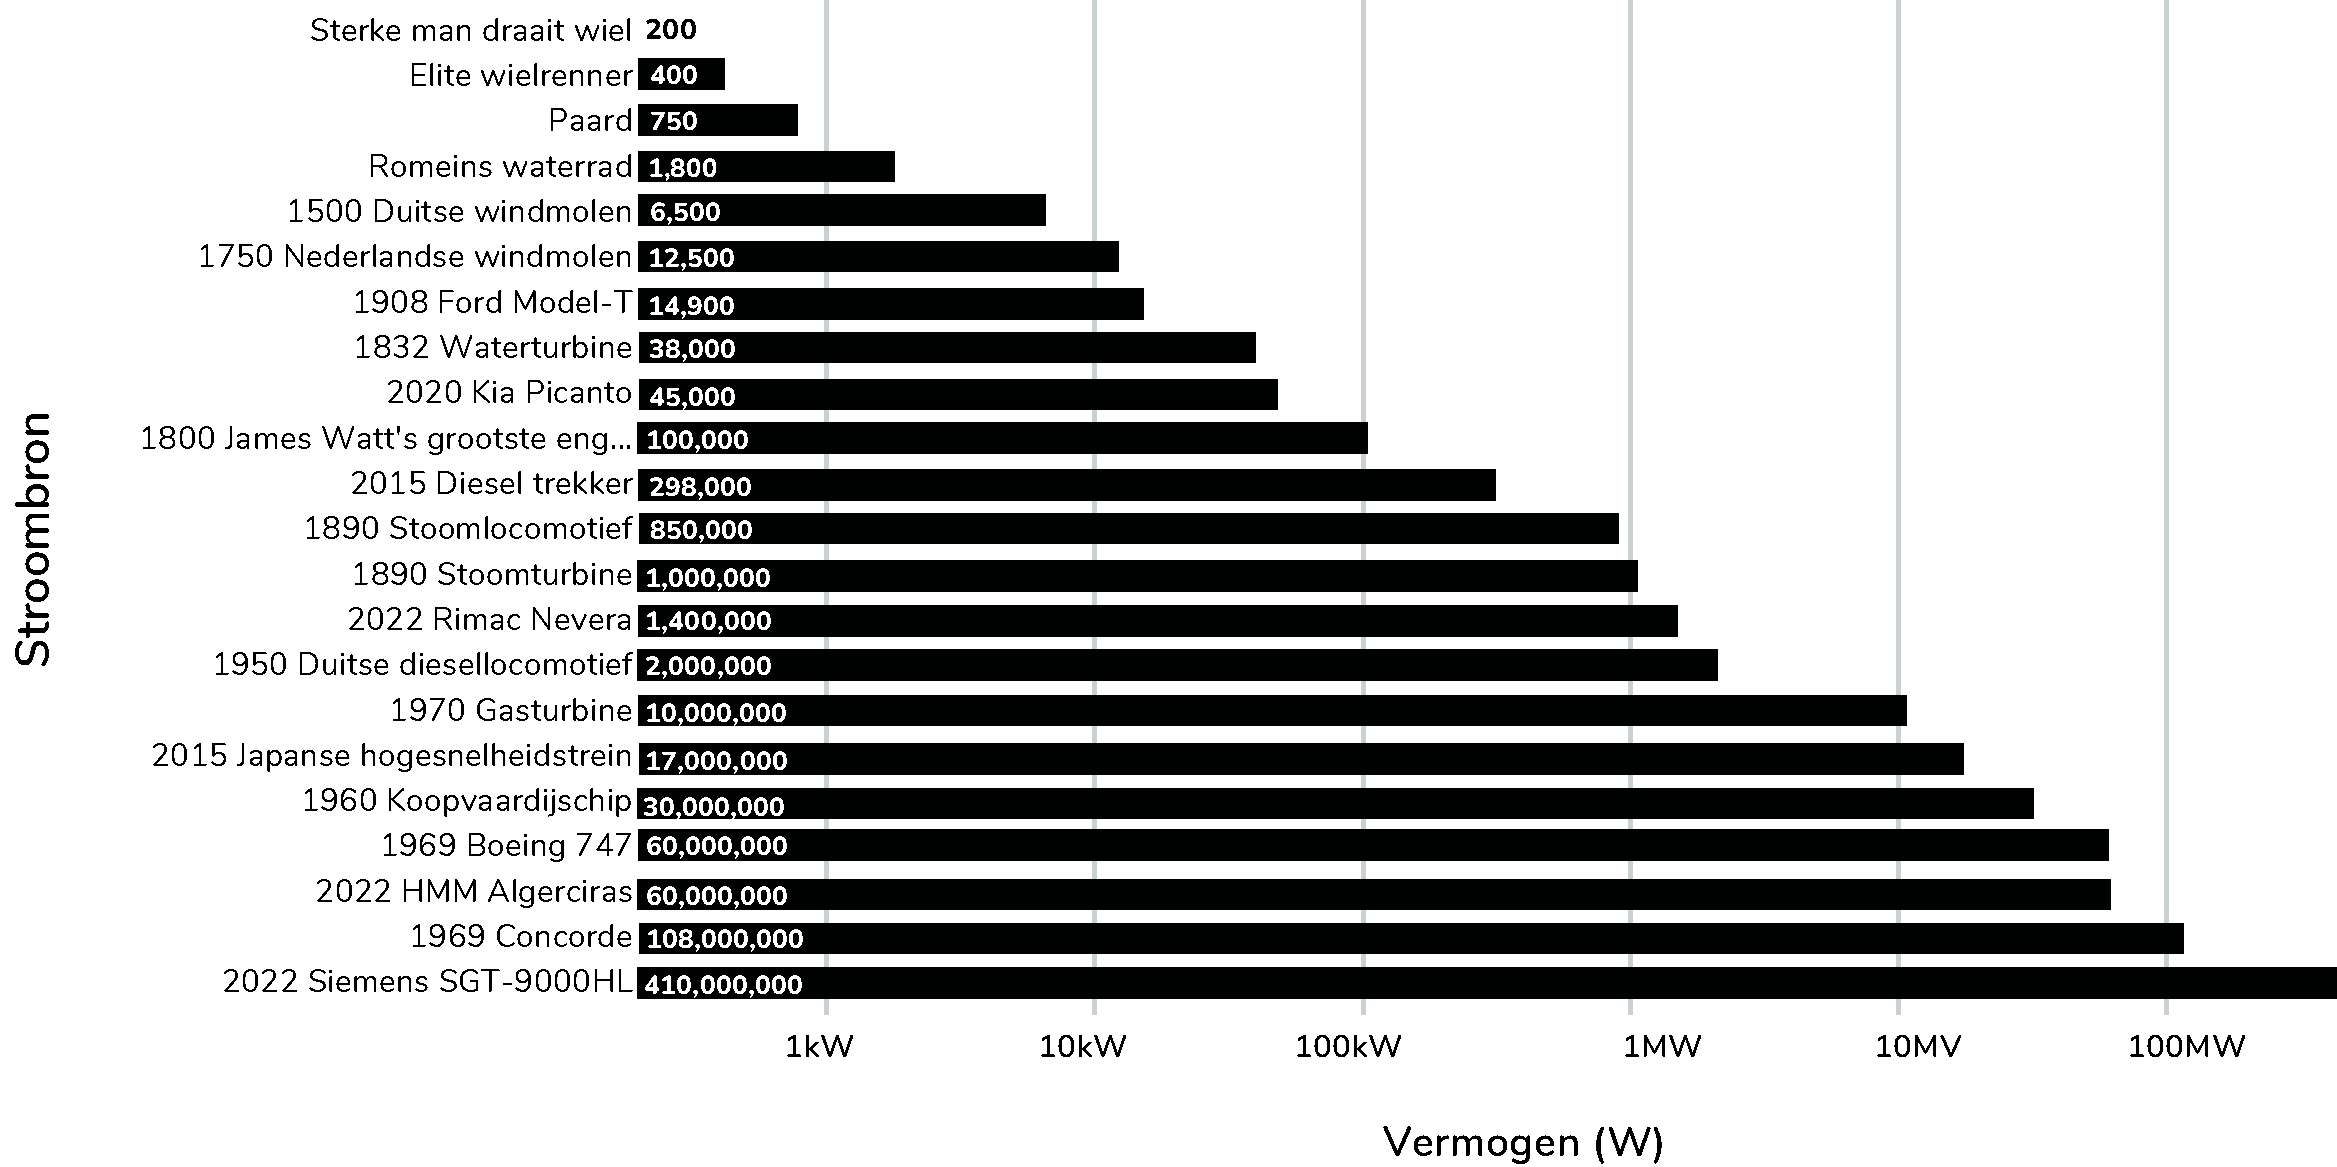
\includegraphics[width=\textwidth]{figures/fig9.pdf}
    \caption[Maximale energieproductie gedurende de afgelopen 3.000 jaar]{Maximale energieproductie gedurende de afgelopen 3.000 jaar}
    \label{fig9}
\end{figure}

Een paard kan ongeveer 750 watt aan vermogen produceren, en een topwielrenner kan ongeveer 400 watt produceren gedurende ongeveer een uur. De Ford Model-T produceerde op volle snelheid 14,9 kW in 1908. Een moderne compacte auto zoals de Kia Picanto produceert ongeveer 45 kW. De krachtigste sportwagen ter wereld, de Rimac Nevera, produceert meer dan 1,4 MW aan vermogen. Rond 1890 draaide een grote stoomlocomotief op volle snelheid 850 kW. In 1950 leverde een krachtige Duitse diesellocomotief 2MW, en in 2015 leverde een snelle Japanse trein 17 MW. In 1960 draaide een Japanse diesel aangedreven koopvaardijschip op 30 MW, terwijl in 1969 een Boeing 747 op 60 MW draaide, en de vier motoren van de supersonische Concorde 108 MW zouden produceren bij een kruissnelheid van 2.400 km/u. De motor van de HMM Algeciras levert 60 MW. Van het paard tot de HMM Algeciras en Boeing 747 heeft de mensheid een 80.000-voudige toename in het vermogen voor vervoer gezien.

Smil vergelijkt ook het maximale vermogen op het land door de tijd. Terwijl een boer die een koolveld schoffelde 50W zou produceren, zou een boer die met twee kleine paarden ploegde 1.000 W tot zijn beschikking hebben. Met een kleine tractor kon een boer in 1950 oogsten met 50 kW aan vermogen tot zijn beschikking. En in 2015 kon een boer met een grote dieseltrekker beschikken over 298 kW aan vermogen. In drie eeuwen van technologische vooruitgang is het vermogen dat een boer tot zijn beschikking heeft, 6.000 keer zo groot geworden.

Voordat koolwaterstoffen bestonden, kon de mensheid slechts beperkte hoeveelheden bruikbare energie gebruiken, en alleen in de buurt van waterraderen en windmolens. Met koolwaterstoffen kunnen op elk moment en overal grote hoeveelheden energie worden opgewekt. Dit maakt het mogelijk om groeiende bevolkingscentra te ondersteunen, handel tussen deze bevolkingscentra te vergroten en de arbeidsproductiviteit te verhogen.

Alex Epstein brengt een overtuigend argument voor hoe koolwaterstofbrandstoffen de basis vormen voor moderne welvaart.\autocite{97} Tot de zestiende eeuw was het leven overal voornamelijk afhankelijk van het verbranden van hout voor de energievoorziening. In vergelijking met moderne koolwaterstoffen bevat hout veel minder energie per eenheid gewicht. Nadat het gebruik van steenkool in de zestiende eeuw startte, gevolgd door olie\index{olie} en gas, nam de hoeveelheid beschikbare energie per persoon enorm toe, en daarmee ook onze levenskwaliteit. Om het echte voordeel van energie voor ons leven te visualiseren, nodigt Epstein ons uit om de energie die we vandaag verbruiken te zien in het licht van het energieverbruik van mensen die taken voor ons uitvoeren. Volgens die maatstaf vindt hij dat de gemiddelde Amerikaan dagelijks over 186.000 calorieën beschikt, of het energie-equivalent van 93 mensen. Vóór moderne brandstoffen was deze hoeveelheid energie zelden voor iemand beschikbaar. Alleen de rijkste koningen konden dromen van het hebben van zoveel energie tot hun dagelijkse beschikking, hetzij in de vorm van brandbaar hout hetzij van tot slaaf gemaakte mensen.

\begin{figure}[!htb]
\centering
    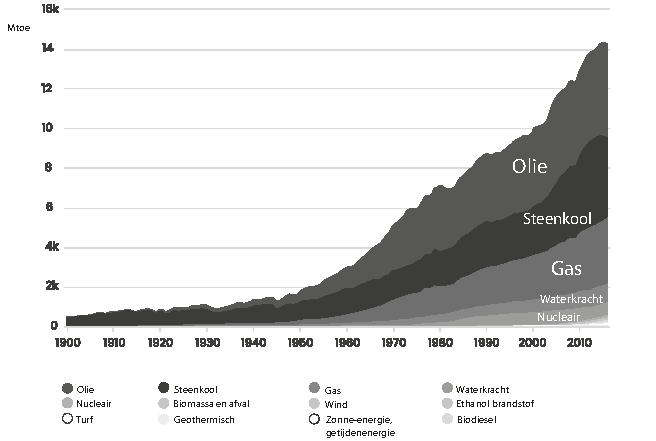
\includegraphics[width=\textwidth]{figures/fig10.pdf}
\caption[Wereldwijd primair energieverbruik]{Wereldwijd primair energieverbruik\footnotemark}
\label{fig10}
\end{figure}
\footautocite{98}

\begin{figure}[!htb]
\centering
    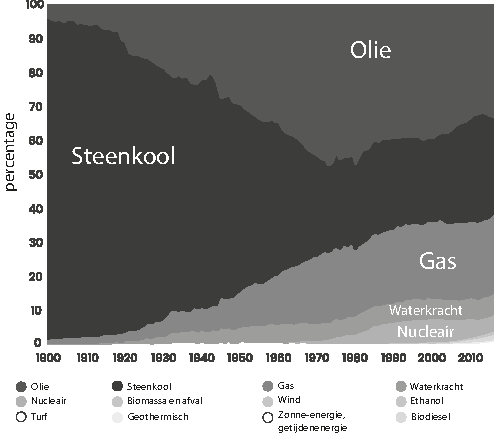
\includegraphics[width=\textwidth]{figures/fig11.pdf}
\caption[Wereldwijd primair energieverbruik, procentueel]{Wereldwijd primair energieverbruik, procentueel\footnotemark}
\label{fig11}
\end{figure}
\footautocite{99}

De Industriële Revolutie, die wereldwijd de levensstandaard transformeerde, was onlosmakelijk verbonden met de uitvinding van de stoommachine en het massale gebruik van kolen om de productiviteit van werknemers te verhogen. Tot het begin van de twintigste eeuw was steenkool de belangrijkste energiebron. De uitvinding van de interne verbrandingsmotor maakte een massaal gebruik van olie\index{olie} mogelijk, die per gewichtseenheid meer energie levert en daarom efficiënter te vervoeren en in transport te gebruiken is. De twintigste eeuw zag een snelle stijging van het wereldwijde gebruik van olie\index{olie}, en in de tweede helft van de twintigste eeuw groeide het gebruik van gas het snelst. Tegenwoordig is ongeveer 80\% van het wereldwijde energieverbruik afkomstig van deze drie koolwaterstofbrandstoffen.

Naarmate technologie verbetert en de levensstandaard stijgt, verwachtten we meer verschuiving naar natuurlijk gas voor energieopwekking, omdat het de minste vervuiling veroorzaakt van alle koolwaterstofbrandstoffen. Desondanks zal er realistisch gezien nog steeds een enorme vraag zijn naar vermogen uit steenkool. Dit komt doordat de enige praktische alternatieven voor veel mensen over de hele wereld laag energetische bronnen zijn, die onbetrouwbaar en niet continu beschikbaar zijn. Steenkool is goedkoop en de technologieën die worden gebruikt om er energie uit op te wekken zijn al decennia lang geperfectioneerd. Moderne schone steenkooltechnologie verlaagt de hoeveelheid schadelijke emissies die door het verbruik ervan wordt veroorzaakt drastisch. De voordelen van betrouwbare energie zijn aanvaardbaar gebleken voor de overgrote meerderheid van mensen die zich verplaatsen naar gebieden met steenkoolcentrales en betrouwbare energie, en weg van gebieden zonder steenkoolcentrales en betrouwbare energie.

In 1802 bouwde Richard Trevithick de eerste werkende spoorweg-stoom\-loco\-motief. Deze gebruikte kolen om treinwagons te laten rijden. Rond dezelfde tijd werd de stoomboot uitgevonden. Die werkte volgens hetzelfde principe. In 1885 werd de auto uitgevonden en in 1902 het vliegtuig. Deze technologieën hebben gedurende meer dan twee eeuwen de kosten van transport verlaagd en de beschikbaarheid ervan verhoogd. Het vervoer van goederen kost vandaag de dag nog maar een fractie van wat het vroeger kostte vóór de komst van koolwaterstofenergie. Hierdoor is onze handelscapaciteit aanzienlijk gegroeid. Ook is de wereldwijde arbeidsdeling\index{arbeidsdeling} enorm toegenomen, wat de menselijke productiviteit verder heeft verhoogd.

Het moderne kapitalisme\index{kapitalisme} en de wereldwijde arbeidsdeling\index{arbeidsdeling} die in de negentiende eeuw ontstonden, zouden simpelweg onmogelijk zijn geweest zonder het gebruik van energiebronnen die zijn gebaseerd op koolwaterstoffen. Deze energiebronnen verhoogden de arbeidsproductiviteit en levensstandaard aanzienlijk. Zonder deze energiebronnen om moderne motoren en machines van brandstof te voorzien, zou de arbeidsproductiviteit niet zijn gestegen tot het punt waarop arbeiders veel meer waarde konden produceren dan ze nodig hadden om te overleven. Hierdoor hadden ze een aanzienlijk aantal middelen om met anderen te verhandelen. De accumulatie van kapitaal\index{kapitaal} nam op een fundamenteel andere manier toe nadat deze brandstoffen het voor mensen mogelijk maakten om snel groeiende hoeveelheden energie te gebruiken.

Het contrast tussen verschillende plekken op de wereld, en de veranderingen door de geschiedenis heen, illustreren hoe enorm waardevol toegang tot grote hoeveelheden vermogen is. Onze moderne wereld is grotendeels het product van de ontwikkeling van technologieën die ons regelmatig toegang geven tot toenemende hoeveelheden energie. Moderne beschaving\index{beschaving} en de meeste van haar prestaties zouden niet mogelijk zijn zonder niveaus van energieverbruik die volledig afwijkend zijn van de historische gegevens.

\begin{figure}[!htb]
\centering
    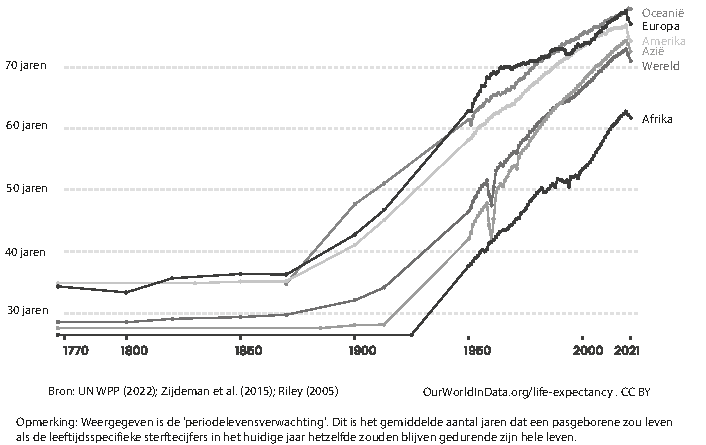
\includegraphics[width=\textwidth]{figures/fig12.pdf}
    \caption[Wereldwijde levensverwachting, 1770-2021]{Wereldwijde levensverwachting, 1770-2021.}
    \label{fig12}
\end{figure}

Gegevens uit 118 landen met bevolkingen groter dan vier miljoen in 2005 laten de correlatie zien tussen energieconsumptie per persoon en verbeterde toegang tot water, levensverwachting, kindersterfte, gemiddeld aantal schooljaren, elektrificatie en bruto nationaal inkomen. \autocite{100} De relaties zijn zeer duidelijk: hoe meer een samenleving in staat is energie te benutten en te verbruiken, hoe beter het in staat is om te voorzien in de basisbehoeften van het moderne leven.

Als we beter naar het bbp kijken, is de relatie zeer duidelijk en al heel lang aanwezig: een groter energieverbruik heeft een sterke correlatie met grotere economische productie\index{productie}, en daardoor een hogere levensstandaard, zoals duidelijk is te zien in Figuur 13.

\begin{figure}[H]
\centering
    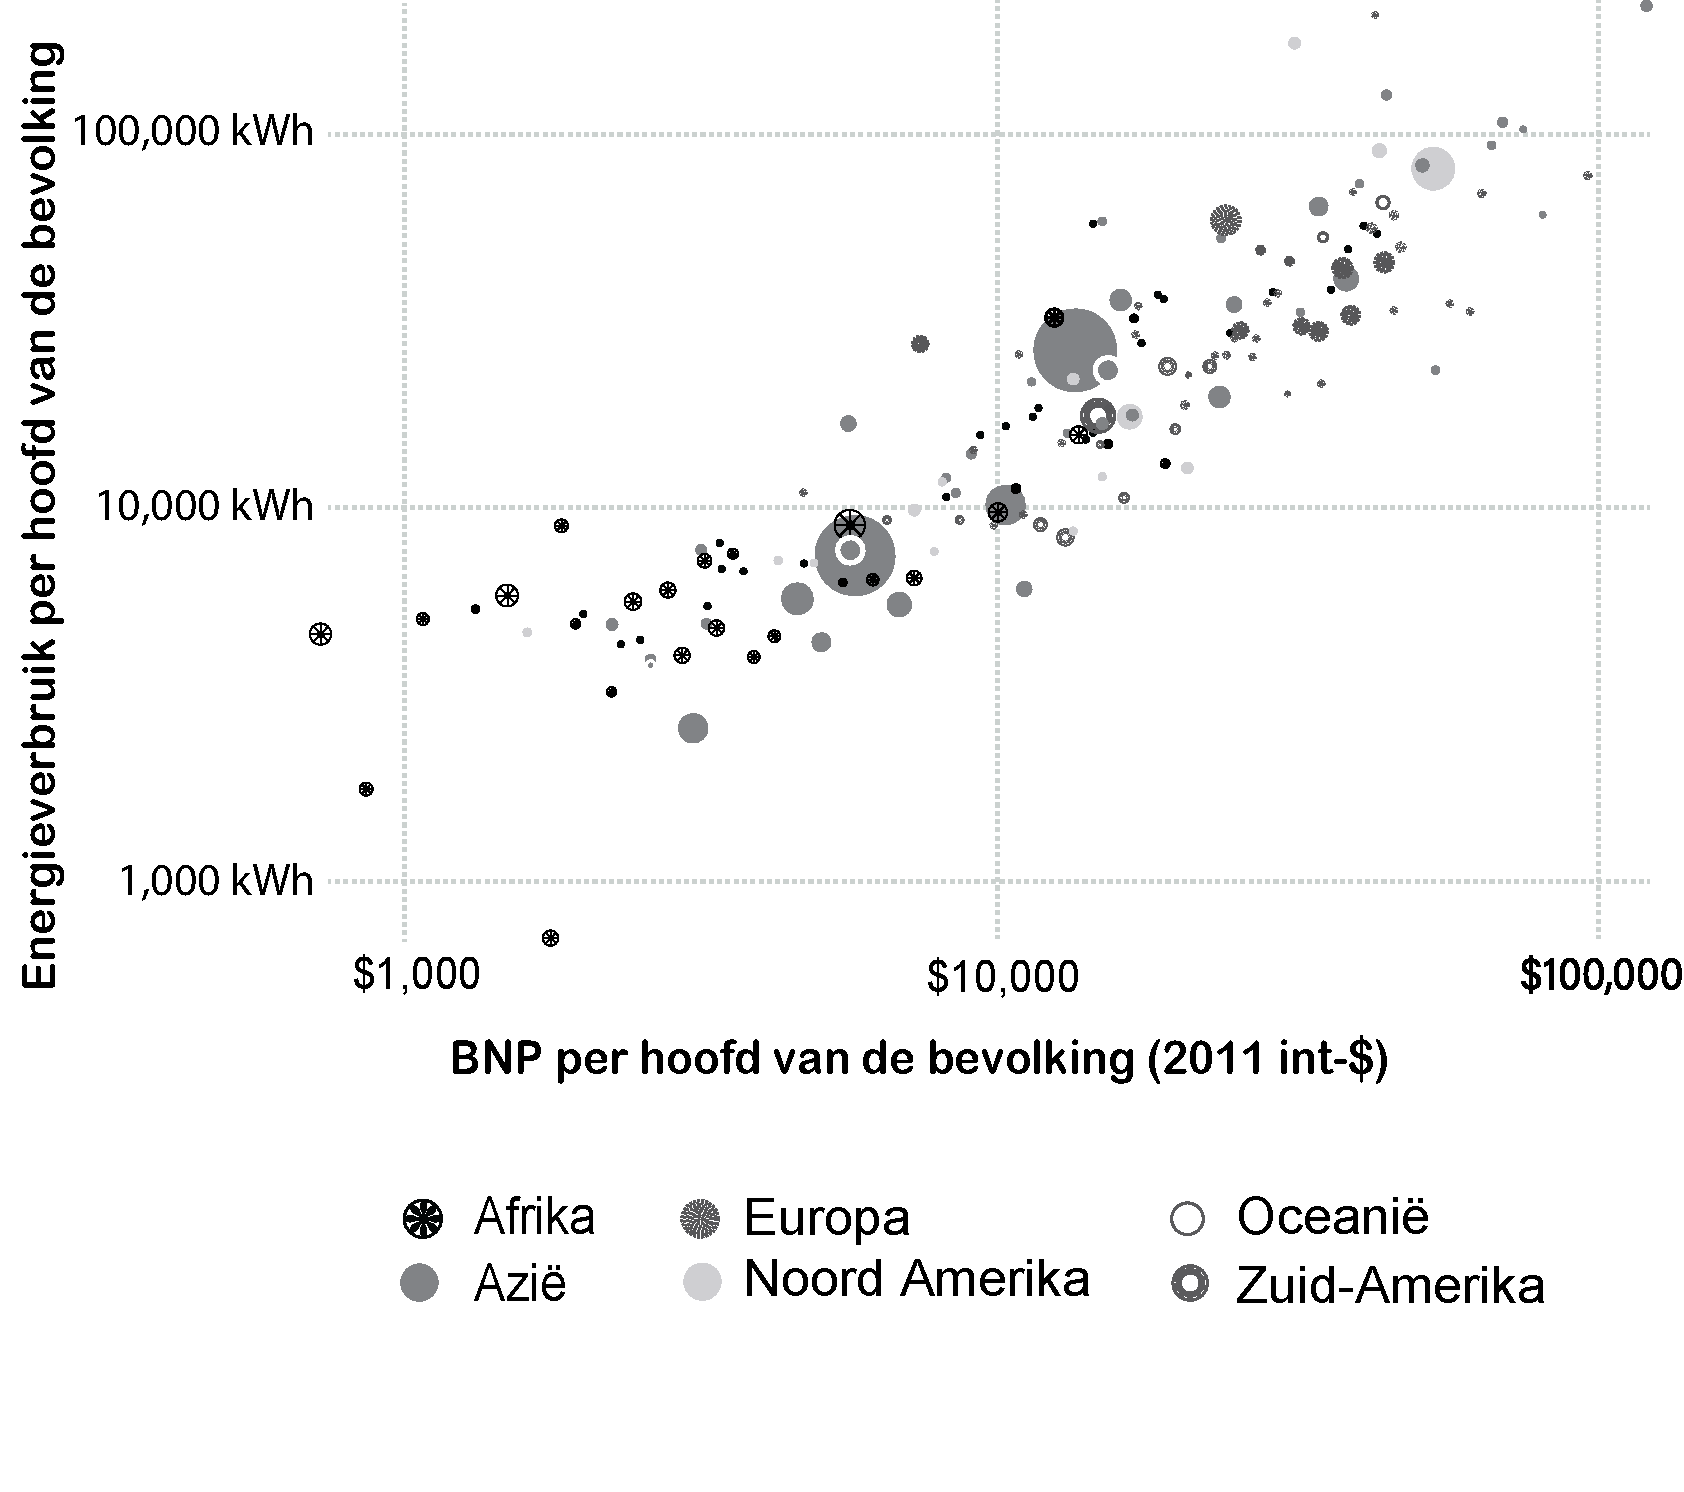
\includegraphics[height=8cm]{figures/fig13.pdf}
    \caption[Energieverbruik per persoon versus bnp, 2015]{Energieverbruik per persoon versus bnp, 2015\footnotemark}
    \label{fig12}
\end{figure}
\footautocite{101}

\begin{figure}[H]
\centering
    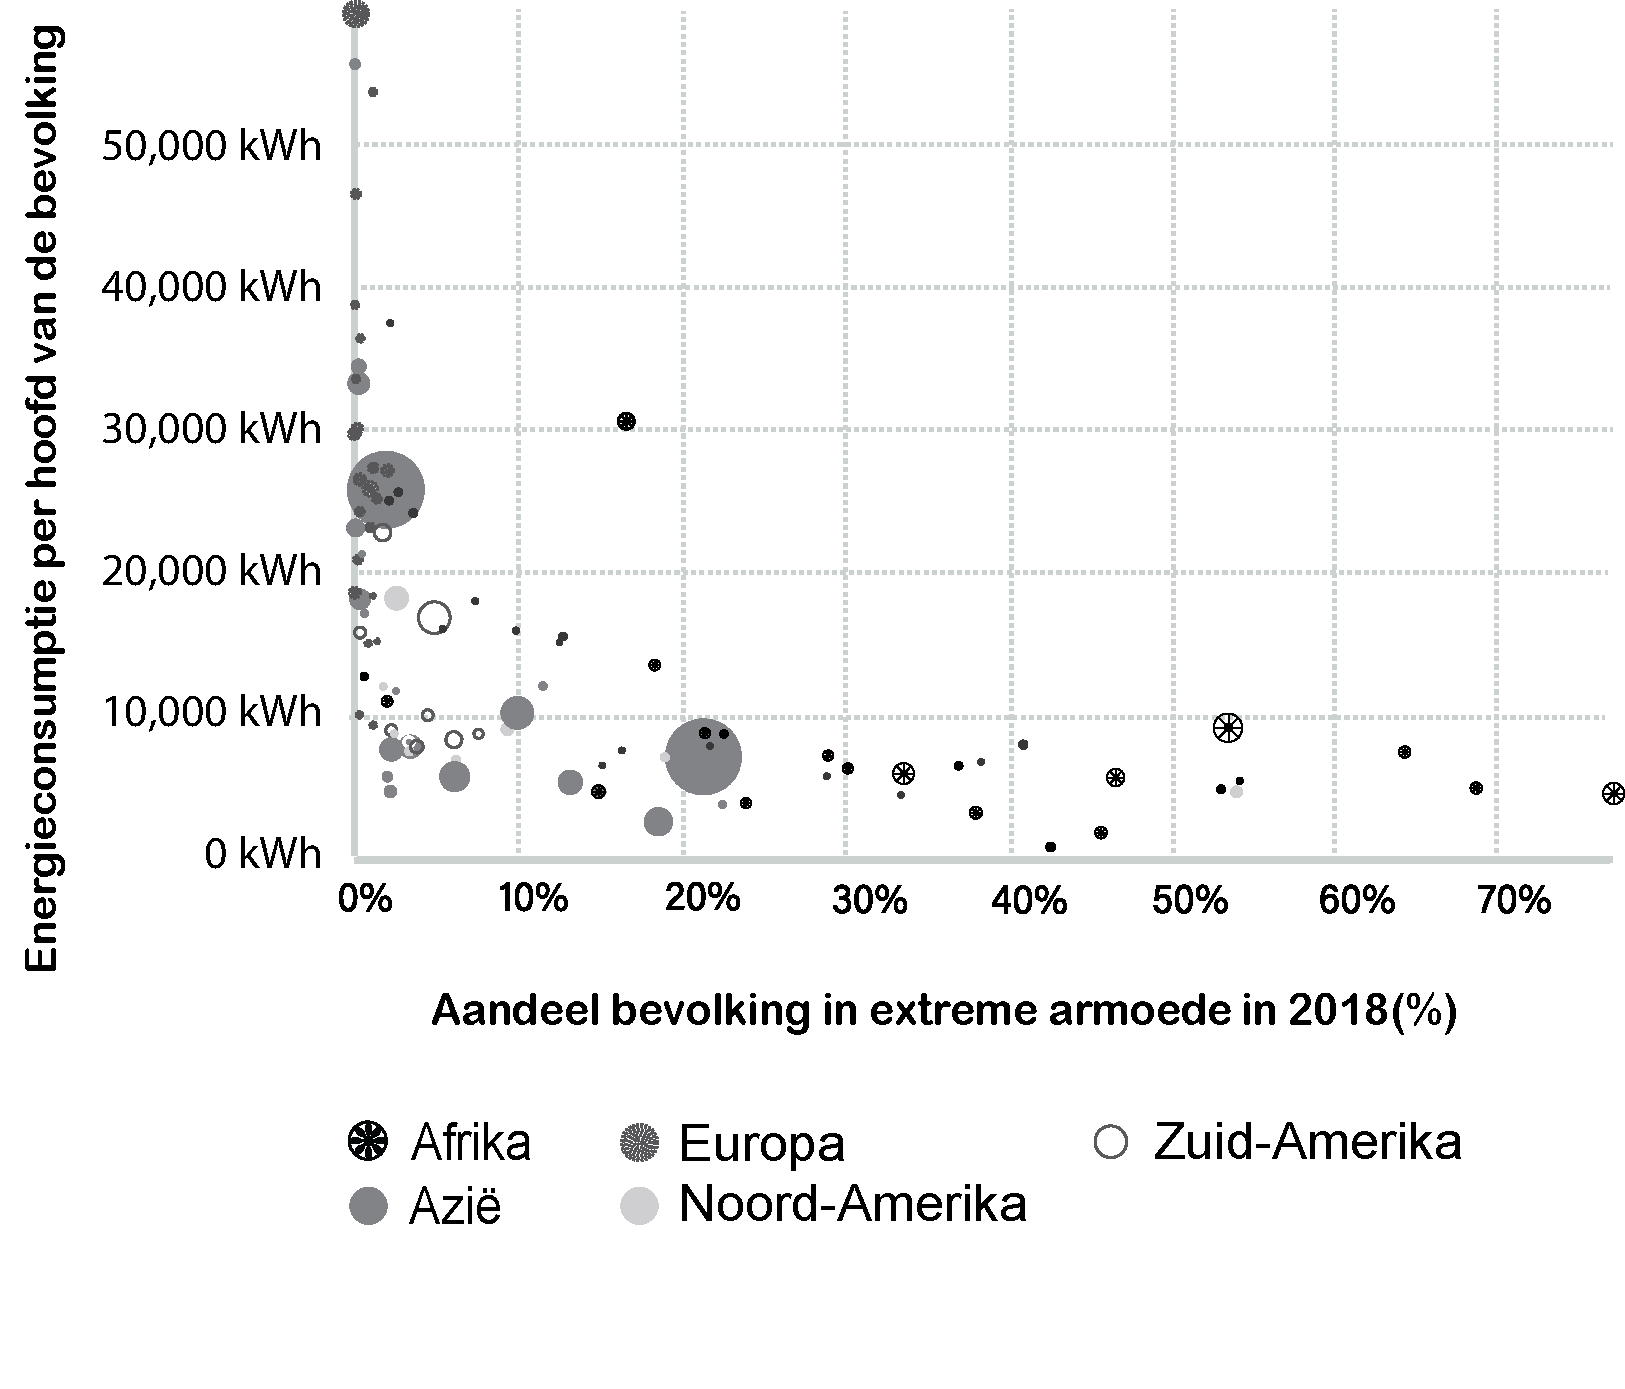
\includegraphics[height=8cm]{figures/fig14.pdf}
    \caption[Energieverbruik per persoon versus percentage van de bevolking in extreme armoede]{Energieverbruik per persoon versus percentage van de bevolking in extreme armoede\footnotemark}
    \label{fig12}
\end{figure}
\footautocite{102}

Figuur 14 toont de relatie tussen het energieverbruik per persoon en het deel van de bevolking dat in extreme armoede leeft. Geen enkel land dat extreme armoede heeft uitgeroeid, verbruikt minder dan 10.000 kWh per hoofd van de bevolking per jaar. En geen enkel land waarin meer dan 20\% van de bevolking in extreme armoede leeft, verbruikt meer dan 10.000 kWh per hoofd van de bevolking per jaar.

De vooruitgang van de mensheid is aangedreven door technologische ontwikkelingen die de energie opgeslagen in koolwaterstofbrandstoffen vrijmaken. Het feit dat de meeste mensen vandaag de dag beschermd leven tegen de meeste gevaren van de natuur, warm kunnen blijven in de winter, en sneller kunnen reizen dan als ze zouden lopen, is het resultaat van innovaties tijdens de Industriële Revolutie. Deze gaven ons diverse soorten motoren om toegang te krijgen tot de energie in de drie belangrijkste koolwaterstofbrandstoffen: steenkool, olie\index{olie}, en gas. Zoals Philip Cross het verwoordde:

\begin{blockquotebox}
    De geschiedenis van economische ontwikkeling is de geschiedenis van de hoeveelheid energie die onder menselijke controle is gebracht.Economische historici hebben de nauwe relatie opgemerkt tussen economische groei en energieverbruik naarmate we meer energie voor ons aan het werk zetten. De Amerikaanse econoom Deirdre McCloskey noemde de toename van het energieverbruik dat rond 1800 begon ``de Grote Verrijking'', beter bekend als \textit{The Great Enrichment}. De voordelen voor de mensheid zijn enorm geweest, de levensverwachting is verlengd, de voedselproductie is verhoogd om de groeiende bevolking te ondersteunen, en de levensstandaard voor de meeste mensen is verhoogd tot niveaus waar zelfs leden van het koningshuis een paar eeuwen geleden niet van konden dromen.
    \par\vspace{1em}\noindent
    De overleden Italiaanse economiehistoricus Carlo Cipolla schreef zowel de Agrarische Revolutie duizenden jaren geleden als de Industriële Revolutie, die aan het einde van de achttiende eeuw begon, toe aan de hoeveelheid energie die werd gebruikt. In de Agrarische Revolutie gingen mensen over van jagen en verzamelen naar het cultiveren en temmen van de energie in planten en dieren, ook al zijn meeste planten en dieren geen erg efficiënte omzetters van energie. Vuur, wind en water verhoogden ook de energie die mensen tot hun beschikking hadden. Na verloop van tijd werden mensen efficiënter in het gebruik van al deze energiebronnen, door middel van rudimentaire landbouwwerktuigen, irrigatie, open haarden, watermolens en zeilboten.
    \par\vspace{1em}\noindent
    Fossiele brandstoffen speelden een verwaarloosbare rol in de energievoorziening tot de Industriële Revolutie. Hoewel alles op de planeet een mogelijke energiebron is, bleken fossiele brandstoffen bijzonder efficiënt en handig om te voldoen aan de energie-eisen van industrialisatie. In de woorden van Cipolla kan de Industriële Revolutie worden beschouwd als ``het proces waarbij de grootschalige exploitatie van nieuwe energiebronnen door middel van anorganische omzetters in gang werd gezet''. Steenkool was de eerste wijdverbreide bron van anorganische energie. Het aandeel ervan steeg van 10 procent van de energievoorziening in Groot-Brittannië in 1560 tot 60 procent in 1750. Dit resulteerde in het beëindigen van de ontbossing van Groot-Brittannië. Dit startte een cumulatief proces, waarbij een groeiende energievoorziening meer economische groei aanwakkerde. Dit stimuleerde op zijn beurt het onderwijs\index{onderwijs}, wat leidde tot de ontdekking van nieuwe energiebronnen, met name andere fossiele brandstoffen.
    \par\vspace{1em}\noindent
    De eerste commerciële toepassing van koolwaterstofbrandstoffen was kerosine om licht te maken en zo een einde te maken aan onze eeuwig terugkerende val in duisternis na zonsondergang. (Dit stopte de grootschalige jacht op walvissen, waarvan de olie\index{olie} tot dan toe de voornaamste bron van binnenverlichting was.) De VS liepen voorop in de exploitatie van olie\index{olie} in de 19e eeuw, een rol die ze vandaag de dag opnieuw op zich neemt dankzij innovatieve technologieën voor de ontwikkeling van schalie-afzettingen. 1860 is het olietijdperk door de ontwikkeling van boortechnologie in Pennsylvania echt van start gegaan.\footnotemark
\end{blockquotebox}
\footautocite{103}

Terwijl mensen nieuwe technologieën blijven ontdekken om energie te gebruiken voor onze doeleinden, verlagen we de reële energiekosten. Fouquet schat in een studie naar de energieprijzen in het Verenigd Koninkrijk tussen 1300 en 2000 dat de verwarmingskosten met meer dan 80\% zijn gedaald. De kosten van energie zijn gedaald met 94\%, die van  vrachtvervoer met 95\%, van passagiersvervoer met 91\% en de kosten voor verlichting zijn gedaald met 99,98\%. Deze dalingen worden geïllustreerd in Figuren 15 en 16.\autocite{104}

\begin{figure}[!htb]
\centering
    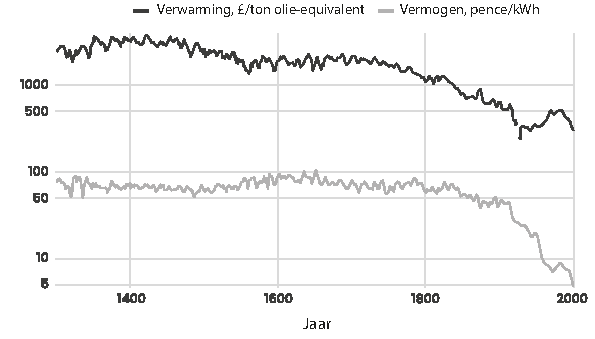
\includegraphics[width=\textwidth]{figures/fig15.pdf}
    \caption[Kosten van verwarming en energie in het Verenigd Koninkrijk, 1300-2000.]{Kosten van verwarming en energie in het Verenigd Koninkrijk, 1300-2000}
    \label{fig15}
\end{figure}

\begin{figure}[!htb]
\centering
    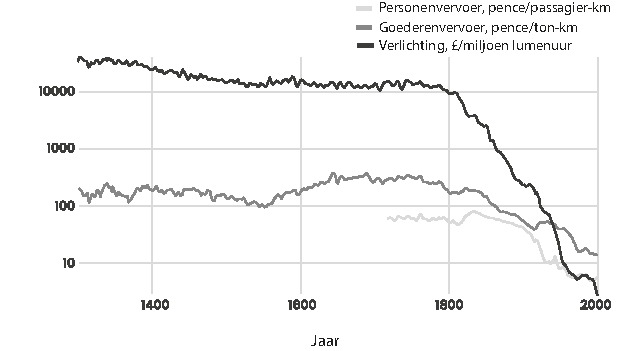
\includegraphics[width=\textwidth]{figures/fig16.pdf}
    \caption[Kosten van verlichting en transport in het Verenigd Koninkrijk, 1300-2000]{Kosten van verlichting en transport in het Verenigd Koninkrijk, 1300-2000}
    \label{fig16}
\end{figure}


\hypertarget{alternatieven-voor-vermogen-uit-koolwaterstof}{%
\section{Alternatieven voor vermogen uit koolwaterstof}\label{alternatieven-voor-vermogen-uit-koolwaterstof}}

Ondanks de verbazingwekkende en onmiskenbare voordelen die hoogwaardige koolwaterstoffen onze wereld hebben gebracht, gelooft een meerderheid van de economen en het publiek dat deze vervangen moeten en zullen worden door alternatieve energiebronnen. Deze afkeer ontstond initieel op basis van de prijsstijgingen van koolwaterstofbrandstoffen in de jaren `70, veroorzaakt door inflatoir monetair beleid, en maakte doemdenkers populair die voorspelden dat we op het punt stonden om deze enorm overvloedige brandstoffen uit te putten. Toen de productie\index{productie} decennia lang bleef toenemen en bewezen reserves\index{reserves} zelfs nog meer groeiden, is deze specifieke hysterie afgenomen. Maar de anti-koolwaterstofhysterie heeft een nieuwe reden gevonden. Onduidelijk en ontoetsbaar pseudowetenschappelijk bijgeloof over broeikasgasemissies als de regelknop voor het weer op aarde zijn nu de reden waarom we van koolwaterstoffen af moeten en over moeten stappen naar ``duurzame''  alternatieven, zoals wind, zon en biobrandstoffen. Ik betoog dat de vijandigheid van de moderne door de overheid\index{overheid} gefinancierde wetenschap tegenover koolwaterstofbrandstoffen zijn wortels heeft in het inflatoire monetaire beleid. Dit beleid verhoogt niet alleen de prijzen van deze essentiële brandstoffen, maar stelt de overheid\index{overheid} ook in staat om de wetenschap te financieren en te dicteren. De overheid\index{overheid} wil brandstofvrije alternatieven promoten, omdat deze minder gevoelig zijn voor monetaire inflatie\index{inflatie} dan energierijke brandstoffen die op de wereldmarkt worden geproduceerd.

Promotors van wind- en zonne-energie beweren vaak dat deze energiebronnen goedkoper zijn dan koolwaterstoffen, omdat hun ``brandstof''  gratis is -- er zijn immers geen kosten verbonden aan zonlicht en wind. Maar dit is een goed voorbeeld van een gebrekkig economisch\index{economisch} redeneren, omdat het geen marginale beslissingen analyseert. Marginale analyse kan ons helpen het onoplosbare probleem met wind- en zonne-energie als alternatieven voor koolwaterstoffen te begrijpen. Energie wordt niet als geheel of abstract gekocht; het wordt aan de marge gekocht, in specifieke hoeveelheden, met bepaalde intensiteiten, voor een bepaalde tijd. Energie zelf is niet het economische goed, maar vermogen is dat wel. De geavanceerde machines die onze moderne beschaving\index{beschaving} mogelijk maken, hebben stroom nodig die op aanvraag en in specifieke, gecontroleerde intensiteiten geleverd kan worden. De stroom die windmolens en zonnepanelen leveren is echter onvoorspelbaar en komt in vlagen, aangezien deze energie alleen beschikbaar is wanneer de wind waait of de zon schijnt. In tegenstelling hiertoe zijn koolwaterstofenergiebronnen gemakkelijk vervoerbaar en op te slaan, wat betekent dat ze in grote hoeveelheden aanwezig kunnen zijn wanneer en waar ze nodig zijn. Zodra moderne machines en infrastructuur eenmaal zijn gebouwd, kan koolwaterstofenergie op aanvraag en op de precieze intensiteit die nodig is beschikbaar worden gesteld tegen zeer lage marginale kosten.

Of het nu gaat om het elektriciteitsnet, ziekenhuizen, couveuses, koelkasten, verwarming en koeling, internetservers, talloze online diensten, luchthavens of talloze vormen van moderne infrastructuur; de moderne beschaving\index{beschaving} heeft haar machines nodig om continu te werken, ongeacht de weersomstandigheden. Geen enkel modern bedrijf\index{bedrijf} kan zijn fabrieken, servers of kantoren laten draaien volgens de grillen van het weer. Om hoogproductieve apparatuur te laten functioneren, is een lage marginale energiekost niet alleen nodig, maar ook op elk moment vereist. Hoewel de marginale kosten van hernieuwbare energiebrandstoffen inderdaad gratis zijn als de zon schijnt en de wind waait, zijn ze oneindig als dit niet het geval is. Geen enkele kapitaalinvestering zal de zon eeuwig laten schijnen en de wind altijd laten waaien wanneer een machine energie nodig heeft. Wanneer de zon niet schijnt, zijn de marginale kosten van zonne-energie oneindig, en wanneer de wind niet waait, zijn de marginale kosten van windenergie oneindig. Als wind- en zonne-energie inderdaad als alternatief voor koolwaterstoffen werden gebruikt, zou een moderne industriële samenleving niet langer mogelijk zijn.

Door overheidsbeleid dat zwaar inzet op subsidies, is het gebruik van wind- en zonne-energie toegenomen. Deze afhankelijkheid heeft echter catastrofale gevolgen. Het verlaagt de voorspelbare piekbelasting voor elk individueel nutsbedrijf, aangezien de piekvraag nu kan optreden op een moment dat sommige brandstoffen niet beschikbaar zijn. Voor de volledige capaciteit van de piekbelasting moet men dan ook volledig vertrouwen op koolwaterstoffen. Hierdoor worden investeringen in kostbare wind- en zonne-infrastructuur praktisch overbodig. Hoewel het inderdaad het verbruik van koolwaterstofbrandstoffen kan verminderen, maken de wisselvalligheid en onvoorspelbaarheid van wind- en zonne-energie het beheer en onderhoud van de koolwaterstofcentrales en netwerken duurder en heffen dus grotendeels de gemaakte besparingen op. Om deze reden bestaat stroomopwekking uit wind en zon slechts in de mate waarin het gesubsidieerd is door overheidsuitgaven.

Mensen streven als ze economisch\index{economisch} handelen voortdurend naar manieren om hun productiviteit te verhogen. In de context van energie is dit altijd in de vorm van het verhogen van de energiedichtheid van de krachtbronnen die we gebruiken om aan onze behoeften te voldoen, gemeten in MJ/kg. Om zonne- en windenergie geschikt te maken voor het moderne leven, zou er gebruik moeten worden gemaakt van batterijen. Deze technologie heeft echter een enorm lage energie per gewicht, rond de 0,5 MJ/kg. Dit is ruwweg 1\% van de energiedichtheid van olie\index{olie} of aardgas. Batterijen zijn ook erg duur, en daarom worden ze voornamelijk gebruikt in gebieden waar motoren niet praktisch zijn.

\vspace{-1em}
\hypertarget{energie-en-vrijheid}{%
\section{Energie en vrijheid}\label{energie-en-vrijheid}}

Toen de menselijke productiviteit erg laag was en de technologie primitief, waren er weinig manieren voor mensen om werk te verzetten om in hun behoeften te voorzien, afgezien van hun eigen arbeid. Een van de meest effectieve energiebronnen was de arbeid van andere mensen. Als een mens echter een zeer lage productiviteit had, had hij zijn eigen arbeid nodig om te overleven. Dit betekende dat hij zelden in staat was om anderen te betalen om voor hem te werken, en anderen konden hem zelden betalen. Kansen voor wederzijds voordelige arbeid zouden schaars zijn in zo\textquotesingle n situatie. Als een man de energie van een ander wilde verwerven om in zijn eigen behoeften te voorzien, zou hij waarschijnlijk de ander moeten dwingen om zijn energie te leveren ten koste van zijn eigen behoeften. Slavernij was in een wereld met primitieve energiebronnen een veel voorkomend instituut, omdat het beschikken over de energie van een ander mens bijna een verdubbeling van de totale hoeveelheid beschikbare energie om in je behoeften te voorzien betekende. Lage productiviteit maakt overleven een lijdensweg, en de arbeid van anderen wordt enorm waardevol, wat slavernij winstgevend maakt.

Naarmate de productiviteit toeneemt door de ontwikkeling van technologie en het gebruik van niet-menselijke energiebronnen, wordt het mogelijk voor mensen om in hun behoeften te voorzien door de inzet van toenemende hoeveelheden energie-intensief kapitaal\index{kapitaal} in plaats van de slavenarbeid van anderen. De dringende behoefte aan arbeid van anderen die aanzet hen tot slaaf te maken, neemt af.

Machines kunnen veel van het werk van de slaaf doen en ze veroorzaken minder problemen dan een mens met een constante drang om vrij te zijn. Omdat machines de productiviteit van een werknemer verhogen, is het mogelijk voor hem om aan zijn eigen behoeften en die van een werkgever die het kapitaal\index{kapitaal} levert, te voldoen. Naarmate de machines duurder en een integraler onderdeel van het economisch\index{economisch} productieproces\index{productieproces} worden, neemt het belang en de verantwoordelijkheid van de werknemer toe en wordt slavernij een volstrekt ongeschikte manier om het werk gedaan te krijgen. Slaven die taken met hoge productiviteit moeten uitvoeren en dure machines gebruiken, zijn waarschijnlijk niet gemotiveerd om deze productief in te zetten, en ze kunnen zeer waarschijnlijk sabotage plegen. Naarmate machines en energie de productiviteit van arbeid verhoogden, nam de kans toe dat werknemers op vrijwillige basis in plaats van onder dwang werden ingeschakeld.

In de context van energiearmoede was het erg belangrijk om de beschikking over de energie van een ander mens te krijgen. Maar in de huidige context van energieovervloed, waar een persoon in een rijk, geïndustrialiseerd ontwikkeld land dagelijks de energie van 100 mensen gebruikt, draagt het toevoegen van een extra mens als slaaf weinig marginaal vermogen bij. Naarmate energiebronnen het menselijk leven binnendrongen, verbeterde onze productiviteit en levensstandaard, waardoor het marginale voordeel van het tot slaaf maken van een mens aanzienlijk kromp. Bovendien, naarmate kapitaalopbouw en moderne machines centraler kwamen te staan binnen het productieproces\index{productieproces}, werd de capaciteit van de arbeider om de machines te onderhouden en niet te beschadigen veel waardevoller dan de kracht die zijn handen boden. De inzet van een slaaf voor zijn meester was niet langer waardevol wanneer een machine veel meer goedkopere energie kon leveren voor zwaar werk. De intelligentie en integriteit van werknemers bij het beheer en onderhoud van machines werd veel waardevoller dan hun brute kracht. Het is geen toeval dat de afschaffing van slavernij zich verspreidde met de industrialisatie. Groot-Brittannië leidde de wereld in het afschaffen van de slavernij, juist omdat het wereldwijd met industrialisatie voorop liep. Waar de stoommachine en de elektrische generator kwamen, verdween de slavernij snel. Slavernij bestaat tegenwoordig nog steeds, maar alleen in industrieel primitieve samenlevingen met weinig kapitaalopbouw en energiegebruik. De economie van machines maakt slavernij economisch\index{economisch} veel minder praktisch. Het maakt zwaar werk, dat door slavernij werd geleverd, voor een zeer lage kostprijs beschikbaar, en verhoogt de productiviteit en waarde van de arbeidstijd van een werknemer tot een punt waarop zijn vrijwillige samenwerking waardevoller is dan elke slavenarbeid die hij zou kunnen uitvoeren.

Hoogwaardige machines zijn ook een ondergewaardeerde aanjager van de emancipatie van vrouwen. In een primitieve economie met weinig krachtige machines was menselijke kracht uiterst waardevol, en de sterkste mensen waren het meest productief. Mannen zijn vanwege een groter lichaam met meer spiermassa gemiddeld sterker dan vrouwen en waren daarom waardevoller in arbeid en vrouwen waren afhankelijk van mannen om te overleven. Toen moderne energie-intensieve machines de meeste fysieke taken overnamen, zoals vervoeren, tillen, pompen, ploegen, en beschermen tegen de natuur en dieren, verminderde het belang van fysieke kracht in vergelijking tot de behoefte aan cognitieve kracht. Hierdoor werd het voordeel dat mannen dankzij hun kracht hadden ten opzichte van vrouwen, verminderd. In een moderne, energierijke economie vereisen de meest productieve en best beloonde banen geen fysieke kracht meer. De sterkste en machtigste mensen in de samenleving zijn niet langer degenen die de meeste hulpbronnen kunnen veiligstellen. Machines doen het zwaarste werk en de hoogste beloningen gaan naar degenen met cognitieve vaardigheden om deze machines te beheren. Vrouwen kunnen in een industriële en informatie-economie veel gemakkelijker onafhankelijk voor hun eigen onderhoud zorgen dan in een primitieve economie. Het is geen toeval dat de emancipatie van vrouwen samengaat met industrialisatie. De rijkste en meest geïndustrialiseerde samenlevingen hebben de best presterende en meest onafhankelijke vrouwen, terwijl in pre-industriële samenlevingen de onderdrukking van vrouwen nog steeds veel voorkomt.


\part{MARKTORDE}
\hypertarget{handel}{%
\chapter{Handel}\label{handel}}

\begin{blockquotebox}
    De essentiële inzichten die de basis vormden voor samenwerking, maatschappij en beschaving\index{beschaving}, en die de mens boven zijn dierlijke oorsprong uit tilden, omvatten het besef dat arbeid, wanneer verricht in het kader van arbeidsdeling\index{arbeidsdeling}, productiever is dan individueel verrichte arbeid, en dat het menselijk intellect in staat is deze realiteit te erkennen.\footnotemark
    \par\raggedleft--- Ludwig von Mises\index{Ludwig von Mises}
\end{blockquotebox}
\autocite{105}

In de voorgaande hoofdstukken hebben we besproken hoe economische handelingen en ruiltransacties kunnen plaatsvinden in afzondering. Arbeid, kapitaalaccumulatie en technologische innovaties in productieprocessen zijn allemaal taken die mensen kunnen gebruiken om hun welzijn te verbeteren zonder interactie met anderen. Ze kunnen arbeid inruilen voor vrije tijd, uitgestelde voldoening inruilen voor directe voldoening en nieuwe technologieën voor oude. Maar mensen zijn sociale dieren, geboren in een familie en een uitgebreide sociale orde, en ze brengen hun leven door in interactie met anderen. Handel drijven met anderen is een instinctief en natuurlijk onderdeel van het leven, iets wat kinderen al op jonge leeftijd doen. De economisch\index{economisch} meest opvallende manier waarop mensen met elkaar kunnen omgaan is door middel van handel of vrij ruilverkeer. In dit hoofdstuk worden de beweegredenen en voordelen van vrij ruilverkeer onderzocht en uitgelegd. De volgende hoofdstukken bouwen hierop voort om een completer beeld te ontwikkelen van onpersoonlijk ruilverkeer in de monetaire marktorde.

Het uitwisselen van goederen met anderen brengt een belangrijke complexiteit in de economische besluitvorming, namelijk het idee dat het andere individu in een economische interactie zijn of haar eigen wil heeft. Bij het doen van economische handelingen met materiële goederen, zoals productie\index{productie}, consumptie\index{consumptie} en kapitaalaccumulatie, heeft het individu alleen te maken met levenloze objecten die geen eigen wil of bewustzijn hebben. Maar in de omgang met anderen wordt het individu geconfronteerd met een andere wil, één met zijn eigen verlangens, voorkeuren, doelen en handelingen.

\textbf{Er zijn slechts twee manieren van interactie tussen mensen: met instemming en onder dwang.} In het geval van wederzijdse instemming, nemen alle betrokkenen deel aan een activiteit die voor hen allen aanvaardbaar is. Ze kiezen er vrijwillig voor om mee te doen aan ruilhandel\index{ruilhandel}, zonder geweld of dreiging om geweld te gebruiken tegen elkaar. Handel, of vrij ruilverkeer, is een uitstekend voorbeeld van een overeenkomst met wederzijds goedkeuren; beide individuen stemmen er vrijwillig mee in om goederen te ruilen, omdat ze zien dat ze voordeel kunnen halen uit de ruil\index{ruil}. Alleen al uit het feit dat twee individuen er vrijwillig voor kiezen om goederen met elkaar uit te ruilen, kunnen we afleiden dat ze allebei verwachten baat bij te hebben bij de transactie. Als ze niet van het resultaat van de ruil\index{ruil} zouden profiteren, zouden ze er niet aan begonnen zijn. Dit is de reden waarom handel vaak een positief-somspel wordt genoemd: de totale winst voor elke deelnemer aan de handel is altijd positief. Anders zouden ze er niet aan meedoen.

Ruilhandel impliceert het vermogen van twee individuen om met hun gezond verstand tot een overeenkomst te komen die voor beide partijen gunstig is, en geen van beiden schaadt. Alleen hun verstand stelt twee mensen in staat om op een manier met elkaar om te gaan die voordelig is voor beiden, omdat het hen in staat stelt om te voorzien wat de voordelen van samenwerking zijn en hoe samenwerking hun situatie zal verbeteren.

Het enige alternatief voor instemming is dwang, het met geweld of het met dreigen met geweld opleggen van de wil van de ene partij aan de andere. Wanneer er sprake is van dwang in een menselijke interactie, kan noodzakelijkerwijs worden geconcludeerd dat een van de partijen in de interactie slechter af is dan wanneer de interactie niet had plaatsgevonden. Als dit niet het geval zou zijn, zou het gebruik van dwang om hem te dwingen in te stemmen met de interactie niet nodig zijn geweest; dan zou hij vrijwillig hebben meegedaan. Dwang kan worden gezien als een nulsomspel, maar het is waarschijnlijker een negatief-somspel. In het geval van diefstal kan de dief een deel van het eigendom van het slachtoffer afpakken, waardoor zijn eigen welzijn toeneemt ten koste van dat van het slachtoffer. Hoewel kwantitatieve economen dit mogelijk een nulsom interactie zouden  noemen, is dit gebaseerd op de foutieve veronderstelling dat waarde objectief is en dat de winst van de dief gelijk is aan het verlies van het slachtoffer. Maar omdat waarde alleen begrepen kan worden als een subjectief fenomeen, kunnen we niet aannemen dat beide individuen het goed evenzeer waarderen.

Een familiestuk dat door een dief op een euro wordt gewaardeerd, kan een buitengewone subjectieve waarde\index{subjectieve waarde} hebben voor de eigenaar, maar omdat de dief het voorwerp niet van het slachtoffer heeft gekocht in een wederzijds onderhandelde ruiltransactie, is de waarde van het voorwerp voor het slachtoffer niet gebleken. De dief heeft niet genoeg waarde aangeboden in ruil\index{ruil}, of zelfs maar geprobeerd te begrijpen wat dat zou kunnen zijn. Het is dus waarschijnlijker dat de waarde die de dief heeft verkregen lager is dan de waarde die het slachtoffer heeft verloren.

Bij geweld kan er zowel bij de aanvaller als de aangevallene fysieke schade ontstaan, waardoor ze beiden te lijden hebben. Geweld is destructief en de toegebrachte schade kan groter zijn dan de buit die het oplevert. Ook brengt het initiëren van geweld altijd de dreiging van vergelding met zich mee. Het plegen van geweld leidt tot een marginale toename van de normalisering van geweld en de kans dat de dader slachtoffer wordt.

Hoe aantrekkelijk de voordelen van dwang ook mogen zijn, ze zullen altijd verbleken in vergelijking met de mogelijke beloningen van samenwerking. Het dierlijke instinct van de mens roept angst op voor de ander, maar het verstand van de mens kan ook de voordelen van samenwerking identificeren, waardoor in feite een beschaafde samenleving ontstaat. Dit kan worden geïllustreerd aan de hand van het voorbeeld van Robinson Crusoë die een andere man met de naam Vrijdag tegenkomt op wat hij dacht dat een verlaten eiland was.

Wanneer Crusoë het pad kruist met Vrijdag, heeft hij eigenlijk twee keuzes: dwang of instemming. Dwang lijkt instinctief verleidelijk: Crusoë zou kunnen proberen zijn wil aan Vrijdag op te leggen, hem te onderwerpen en tot slaaf te maken, of hem te vermoorden en zijn eigendommen af te pakken. Elk van deze mogelijkheden levert winst op voor Crusoë, maar omdat ze ondraaglijk zijn voor Vrijdag, zouden ze zeer waarschijnlijk leiden tot een gewelddadige confrontatie tussen de twee mannen, en de uitkomst zou voor beiden onzeker zijn. Crusoë zou verslagen kunnen worden, tot slaaf gemaakt, of zelf gedood, of hij zou gewond kunnen raken terwijl hij zegeviert. Als hij wint, kan hij misschien alle bezittingen bemachtigen en Vrijdag kunnen onderdrukken als slaaf, maar hij zou zich niet kunnen verzekeren van Vrijdags enthousiaste medewerking om productief werk te leveren, omdat Vrijdag weet dat zijn productie\index{productie} in de eerste plaats ten goede zou komen aan Crusoë. Crusoë zou nooit in staat zijn om Vrijdag te vertrouwen. Hij zou altijd kunnen proberen om hem kwaad te doen. Conflicten en geweld die tot de dood leiden zijn de verwachte uitkomst van dit pad.

Anderzijds, als de twee mannen zouden besluiten om met elkaar samen te werken en elkaar alleen te benaderen op voorwaarden die voor beiden acceptabel zijn, dan zouden ze op de lange termijn waarschijnlijk allebei veel beter af zijn. De materiële bezittingen die Vrijdag op dit moment heeft en die Crusoë zou kunnen inpikken, verbleken bij alle goederen die hij zou kunnen produceren als hij in leven zou blijven en vrij zou zijn om te werken, en op die manier zo productief mogelijk te zijn en samen met Crusoë mee te doen aan een arbeidsdeling\index{arbeidsdeling}.

Als Crusoë en Vrijdag allebei bereid zijn om elkaars soevereiniteit en eigendom te respecteren, kunnen ze op een veilige manier produceren en de goederen die ze produceren uitwisselen. De voordelen die ze kunnen behalen door samen te werken zijn veel groter dan alles wat ze kunnen behalen als ze vijandig en strijdlustig blijven. Ondanks de verbazingwekkende voordelen die zijn te behalen met de inzet van arbeid, kapitaalaccumulatie en technologische innovatie alleen, ligt er een nog veel grotere wereld van mogelijkheden voor mensen open als ze met anderen gaan ruilen. Economen hebben door de eeuwen heen verschillende denkbare hulpmiddelen en constructies bedacht om ons te helpen het belang van handel en het enorm heilzame potentieel ervan te begrijpen. In de rest van dit hoofdstuk worden deze hulpmiddelen toegelicht om te illustreren dat de voordelen van samenwerking ver uitstijgen boven die van conflicten.

\hypertarget{subjectieve-waardering}{%
\section{Subjectieve waardering}\label{subjectieve-waardering}}

De basis voor het begrijpen van handel als economisch\index{economisch} fenomeen, is het concept waarop alle economische redeneringen zijn gebaseerd: subjectieve waardering. Alleen door te begrijpen dat waarde subjectief is, wordt het concept handel mogelijk. Als waarde objectief zou zijn, wat voor baat zouden mensen dan hebben bij ruilhandel\index{ruilhandel}? Waarom zouden ze iets voor iets anders willen ruilen als ze beide goederen precies hetzelfde waarderen? Het marginale nut van de geruilde goederen moet voor beide partijen toenemen. Elke partij krijgt meer voldoening van wat ze verwerven dan van wat ze opgeven.

Mensen kunnen voorwerpen met elkaar ruilen omdat ze verschillende waarderingen toekennen aan dezelfde voorwerpen. Waarde is niet iets wat inherent is aan objecten, noch is het een eigenschap die objecten in een bepaalde duidelijk vaste hoeveelheid krijgen. Waarde wordt toegekend door de menselijke geest en deze waardering is marginaal. Individuen kennen waarde toe aan objecten op basis van de waarde die ze eraan hechten op het specifieke moment en de specifieke plaats waarop ze hun waardebepaling maken. Dit hangt af van een reeks factoren, waarbij de hoeveelheid van deze goederen die ze reeds in bezit hebben vaak het belangrijkste is.

Het is dus heel goed mogelijk dat Crusoë een appel meer waardeert dan een sinaasappel, terwijl Vrijdag meer waarde hecht aan een sinaasappel dan aan een appel. Als Crusoë een sinaasappel bezit en Vrijdag een appel, dan zouden ze allebei profiteren van het ruilen van hun fruit. We kunnen dit begrijpen door na te denken over hun gedrag en door wat we weten over de manier waarop mensen handelen. Als Vrijdag uit eigen beweging de ruil\index{ruil} voorstelt en Crusoë vrijwillig akkoord gaat, kunnen we alleen maar concluderen dat de ruil\index{ruil} hun beider welzijn verbetert: omdat Vrijdag meer waarde hecht aan de sinaasappel dan aan zijn appel en Crusoë meer aan de appel dan aan zijn sinaasappel, profiteren ze allebei van de ruil\index{ruil}.

Een andere manier om te begrijpen waarom handel plaatsvindt, is door te kijken naar de implicaties van de wet van het afnemende marginale nut in de context van interpersoonlijke interactie. Aangezien het marginale nut van elke eenheid van een goed afneemt naarmate de hoeveelheid van het goed toeneemt, volgt hieruit logischerwijs dat individuen mogelijkheden voor ruilhandel\index{ruilhandel} zullen vinden door de goederen waarvan ze er veel van hebben te ruilen tegen de goederen waarvan ze er maar weinig hebben. Als Crusoë een sinaasappelboom heeft en Vrijdag een appelboom, zal ieder waarschijnlijk een grote hoeveelheid van zijn eigen fruit hebben en geen fruit van de ander. Ze zouden het marginale fruit van hun individuele bomen waarschijnlijk veel minder waarderen dan het eerste fruit dat ze van de boom van de ander kunnen krijgen. Crusoë\textquotesingle s sinaasappelboom geeft hem meer sinaasappels dan hij kan eten, en nadat hij het grootste deel van de oogst heeft opgegeten, hebben de laatste sinaasappels weinig waarde voor hem. Misschien wil hij ze niet eens eten. Maar omdat hij geen appels heeft gegeten voordat hij Vrijdag ontmoette, zal de marginale waarde die hij hecht aan de eerste appel die hij van Vrijdag kan krijgen relatief hoog zijn. Vrijdag hecht op zijn beurt heel weinig waarde aan de laatste paar appels die aan zijn boom groeien en zou een sinaasappel van Crusoë\textquotesingle s boom veel hoger waarderen. Door handel kunnen ze allebei iets opgeven waar ze niet veel waarde aan hechten om er iets voor terug te krijgen waar ze meer waarde aan hechten.

Een veel voorkomende misvatting in de economie is het verwarren van waarde en prijs\index{prijs}. Alleen al het feit dat mensen er vrijwillig voor kiezen om te ruilen, laat zien dat deze opvatting onhoudbaar is. Als iemand \$10 betaalt voor een goed, waardeert ze het niet op \$10, ze waardeert het op meer dan \$10 omdat ze vrijwillig \$10 opgeeft in ruil\index{ruil} voor het goed. De verkoper daarentegen waardeert het goed duidelijk op minder dan \$10, omdat hij het vrijwillig opgeeft voor dat bedrag.

Hoewel verschillende subjectieve waarderingen de beweegreden voor handel verklaren, geeft het niet volledig de voordelen en implicaties ervan weer, omdat het zich richt op de beslissingen die over de eindproducten worden genomen. De krachtigere potentiële implicaties voor handel worden duidelijk als we kijken naar het effect dat het heeft op het productieproces\index{productieproces}. Twee belangrijke benaderingen om menselijk handelen\index{menselijk handelen} in interpersoonlijke ruilhandel\index{ruilhandel} te begrijpen zijn de concepten van absoluut voordeel\index{absoluut voordeel} en comparatief voordeel\index{comparatief voordeel}.

\hypertarget{absoluut-voordeel}{%
\section{Absoluut voordeel}\label{absoluut-voordeel}}

Handel komt voort uit verschillen in de subjectieve waardering van eindproducten, maar het is ook een weerspiegeling van verschillen in de productiekosten van verschillende goederen. Zelfs in een primitieve omgeving zonder marktprijzen waarmee je goederen kunt vergelijken, zijn individuen in staat om de verschillen in de economische waarde van verschillende goederen te onderscheiden en mogelijkheden te vinden om hun subjectieve welzijn te verbeteren. Dit kan bijvoorbeeld door middel van transacties waarbij elke partij goederen met lagere productiekosten opgeeft waarvoor zij lagere productiekosten hebben  om goederen te verwerven waarvoor ze hogere productiekosten hebben.

Stel je een situatie voor waarin Crusoë en Vrijdag hun vijandige eerste instincten bedwingen en elkaar in plaats daarvan vreedzaam benaderen. Crusoë ontdekt dat Vrijdag een overvloed aan konijnenhuiden in zijn grot heeft, omdat hij erg goed is in het jagen op konijnen, terwijl Crusoë bedreven is in het vangen van vis. Bij het zien van de overvloed aan konijnenvellen realiseert Crusoë zich dat hij het konijnenvlees graag wil hebben en hij vraagt Vrijdag of hij geïnteresseerd is in het ruilen van een vis voor een konijn. Nadat hij maandenlang alleen maar konijnenvlees heeft gegeten, neemt Vrijdag het aanbod enthousiast aan. Hij kan nauwelijks vissen en elke keer als hij het probeert, verspilt hij veel tijd en slaagt hij er niet in om genoeg vis te vangen om zijn honger te stillen. Maar nu biedt Crusoë hem een vis aan in ruil\index{ruil} voor een konijn, dat voor Vrijdag heel gemakkelijk te vangen is. Vrijdag denkt misschien zelfs dat hij Crusoë uitbuit door een kostbare vis te ontvangen in ruil\index{ruil} voor een konijn dat makkelijk te bemachtigen is, maar Crusoë denkt waarschijnlijk hetzelfde. Hij is eindelijk in staat om een ongrijpbaar konijn te bemachtigen, en het enige wat hij hoeft te doen om er een te krijgen is een van de vele vissen geven die hij gemakkelijk kan vangen. In deze situatie geven beide mannen iets op wat ze goedkoop kunnen produceren om iets te krijgen waar ze veel meer waarde aan hechten. In zekere zin maken ze allebei misbruik van elkaar.

Deze situatie kan worden geïllustreerd met een hypothetisch cijfervoorbeeld. We kunnen de productiemogelijkheden grafisch voorstellen met behulp van een productiemogelijkhedengrens, ook wel bekend als de productiemogelijkhedencurve -- een lijn die alle mogelijke combinaties van twee goederen illustreert die geproduceerd kunnen worden. Stel je voor dat Vrijdag in één dag 8 konijnen of 2 vissen kan vangen, terwijl Crusoë 2 konijnen of 10 vissen kan vangen. Als ze onafhankelijk van elkaar zouden werken en niet zouden samenwerken, dan zouden deze hoeveelheden de respectievelijke limieten vertegenwoordigen van hoeveel ieder van hen dagelijks zou kunnen consumeren. Vrijdag zou ofwel de 8 konijnen kunnen consumeren ofwel de 2 vissen die hij kan vangen, en Crusoë zou ofwel de 2 konijnen kunnen consumeren ofwel de 10 vissen die hij kan vangen. Als ze allebei voor zichzelf zouden besluiten om hun werkdag gelijk te verdelen tussen vissen en jagen, zou Vrijdag de dag afsluiten met 4 konijnen en 1 vis, terwijl Crusoë 1 konijn en 5 vissen zou hebben, zoals te zien is in punt I in Figuur 17. De som voor beiden zou dan 5 konijnen en 6 vissen zijn.

\begin{figure}[!htb]
\centering
    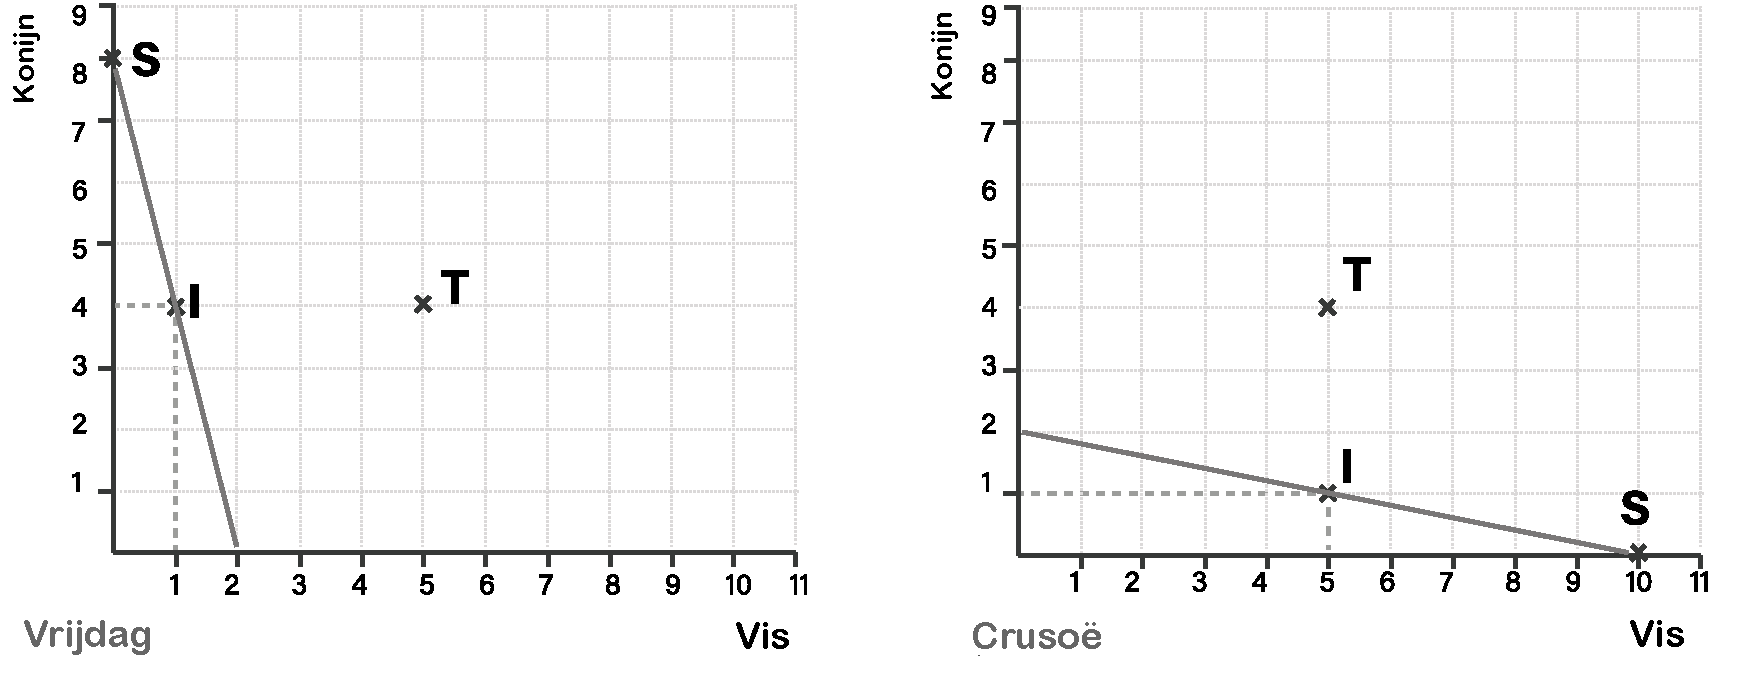
\includegraphics[width=\textwidth]{figures/fig17.pdf}
    \caption[Productiemogelijkheden in isolatie en in handel.]{Productiemogelijkheden in isolatie en in handel}
    \label{fig17}
\end{figure}

Als Crusoë Vrijdag zou aanvallen en proberen te beroven, zou hij misschien al het voedsel dat Vrijdag heeft kunnen meenemen, maar dan zou Vrijdag verhongeren en zou Crusoë niets anders overhouden dan zijn eigen productie\index{productie}, net als in zijn oorspronkelijke staat. Maar als ze zouden besluiten om samen te werken, zouden ze allebei kunnen profiteren van de verschillen in hun vangsten. Omdat Crusoë merkt dat Vrijdag een overvloed aan konijnen heeft, maar niet veel vis, stelt hij voor om wat van zijn konijnen te ruilen tegen de vis van Crusoë. Konijnen zijn er voor Vrijdag in tegenstelling tot vis in overvloed, dus een vis ruilen voor een konijn is zowel voor hem als voor Crusoë een win-winsituatie.

De ruiltransactie laat Vrijdag inzien dat de beste manier om aan vis te komen is om op konijnen te jagen en die te ruilen voor vis, terwijl Crusoë zich realiseert dat hij meer konijnen kan krijgen door te vissen en de vis te ruilen voor konijnen dan door op konijnen te jagen. Het eindresultaat is dat het logisch is dat ze zich specialiseren in de goederen die ze goedkoper kunnen produceren. Als ze zich specialiseren, en Crusoë alleen vis en Vrijdag alleen konijnen vangt, zoals weergegeven in punt S in Figuur 17, dan zou hun gezamenlijke dagelijkse productie\index{productie} 8 konijnen en 10 vissen zijn, wat 3 konijnen en 4 vissen meer is dan ze zouden hebben gehad als ze vijanden waren gebleven. Als ze hun oogst in tweeën delen, krijgen ze elk 4 konijnen en 5 vissen, zoals te zien is in punt T.

Door zich simpelweg te specialiseren in de productie\index{productie} van het goedkopere goed, hebben ze allebei meer vis en konijnen geproduceerd dan wanneer ze elk hun tijd en inspanning hadden verdeeld over de productie\index{productie} van beide. Dit resultaat lijkt bijna een goocheltruc: ze werken allebei evenveel uren en toch hebben ze uiteindelijk allebei meer konijnen en vis te eten en zijn ze allebei beter af. Dit is geen eenmalig voordeel zoals die van de buit na diefstal, maar een duurzame verbetering in hun leven die kan voortduren zolang ze in goede verstandhouding met elkaar blijven handelen. In feite worden ze elke ochtend wakker met een keuze: samenwerken en meer eten of vijandig zijn en minder eten. Door elke persoon in staat te stellen zijn tijd te besteden aan de productie\index{productie} van het goed dat voor hem minder duur is, verhoogt de handel de productiviteit van beide partijen. Als één van hen de ander had gedood, zou de ``winnaar'' nooit zoveel winnen als wanneer hij vrijwillig met de ander zou samenwerken.

\hypertarget{comparatief-voordeel}{%
\section{Comparatief voordeel}\label{comparatief-voordeel}}

De redenering achter absoluut voordeel\index{absoluut voordeel} is intuïtief en gemakkelijk te begrijpen. Elk individu specialiseert zich in wat hij tegen lagere kosten kan produceren, wat leidt tot meer productie\index{productie} van alle goederen. Maar het concept van comparatief voordeel\index{comparatief voordeel} is een meer algemene en krachtige verklaring van de voordelen van handel als gevolg van verschillen in de opportuniteitskosten van goederen, ongeacht de aard en omvang van de verschillen in productiviteit tussen de deelnemers. Ruilhandel kan wederzijds voordelig zijn, zelfs als het ene individu productiever is in de productie\index{productie} van beide betrokken goederen dan de andere persoon, vanwege de verschillen in opportuniteitskosten van goederen voor beide individuen. Het feit dat menselijke tijd het ultieme schaarse goed is, betekent dat samenwerking tussen twee mensen voordelig is voor hen beiden, zelfs als de ene productiever is in het produceren van beide goederen, omdat hun samenwerking hen in staat stelt hun schaarse tijd daar in te zetten waar die het meest productief is.

Stel je voor dat Crusoë in het bovenstaande voorbeeld productiever zou zijn in zowel vissen als jagen, en hij 6 konijnen of 12 vissen per dag zou kunnen produceren, terwijl Vrijdag slechts 4 konijnen of 2 vissen zou kunnen produceren. Dit betekent niet dat de twee geen voordeel kunnen halen uit de arbeidsdeling\index{arbeidsdeling}. Als de twee mannen geïsoleerd hadden geproduceerd en geconsumeerd, en ieder de helft van de dag hadden gejaagd en de andere helft gevist, dan zou Crusoë 3 konijnen en 6 vissen hebben, terwijl Vrijdag 2 konijnen en 1 vis zou hebben, voor een totaal van 5 konijnen en 7 vissen. Als ze samenwerken en zich specialiseren, vangt Vrijdag 4 konijnen en Crusoë 12 vissen, zoals te zien is in punt S. Als ze liever meer konijnen hebben, zou Crusoë een deel van zijn dag kunnen besteden aan jagen, en zouden ze uiteindelijk 5 konijnen en 10 vissen hebben, zoals te zien is in punt S2. In dit geval zouden ze 3 vissen aan hun dagelijkse consumptie\index{consumptie} hebben toegevoegd door zich te specialiseren. Er zijn verschillende andere combinaties van vis en konijnen die ze zouden kunnen produceren, afhankelijk van hun smaak en voorkeur voor beide. Zolang de specialisatie elke producent in staat stelt om zich te concentreren op het goed met de laagste opportuniteitskosten, zouden ze een subjectief waardevollere productie\index{productie} hebben dan wanneer ze individueel zouden produceren.

\begin{figure}[!htb]
\centering
    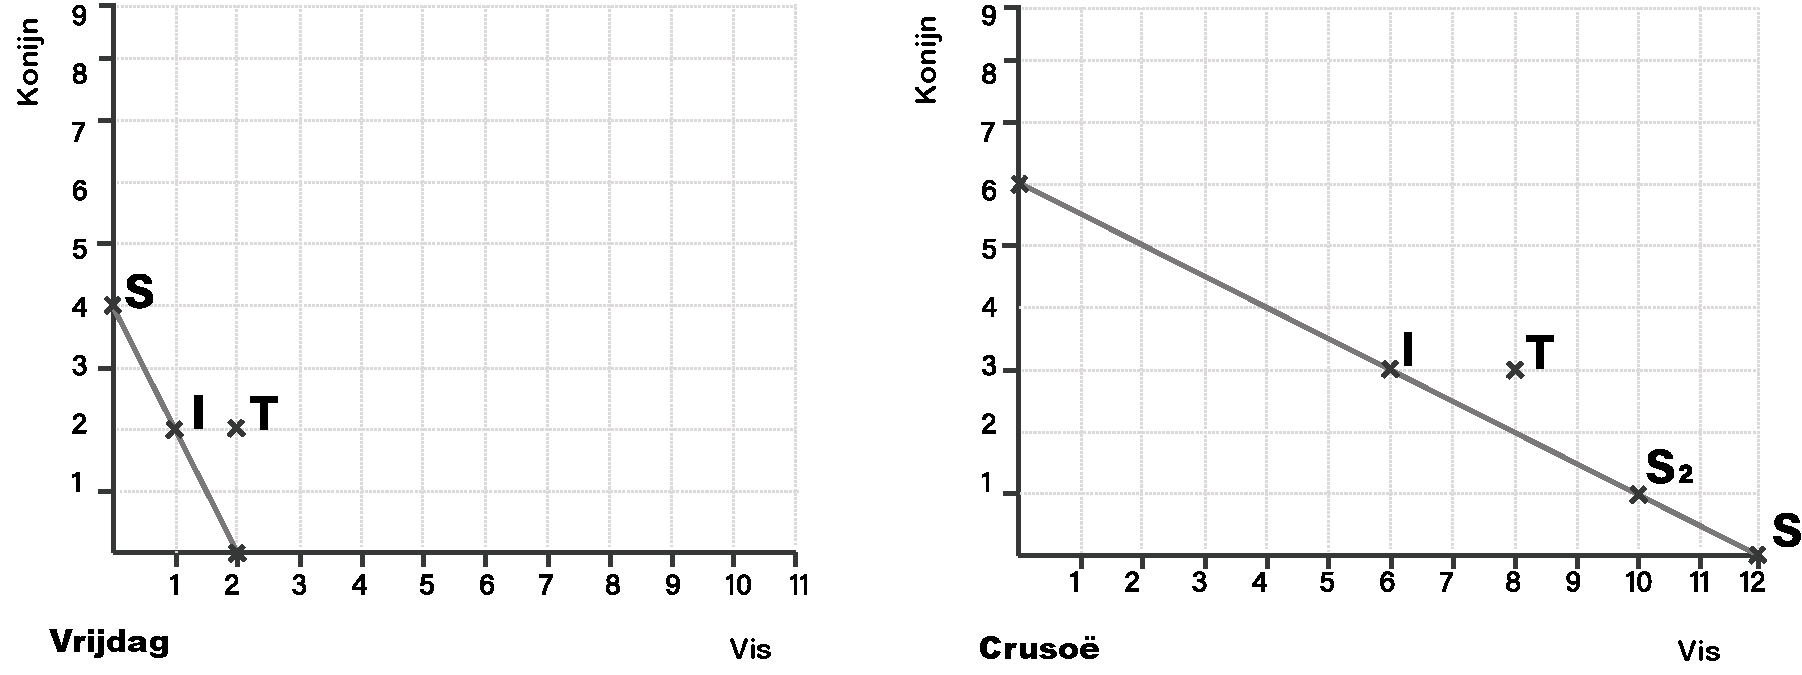
\includegraphics[width=\textwidth]{figures/fig18.pdf}
    \caption[Productiemogelijkheden in isolatie en met comparatief handelsvoordeel]{Productiemogelijkheden in isolatie en met comparatief handelsvoordeel}
    \label{fig18}
\end{figure}

Zowel Crusoë als Vrijdag zouden precies evenveel uren werken, en toch zouden ze meer produceren dan voorheen, ook al is Crusoë productiever in zowel jagen als vissen. Het feit dat de twee mannen verschillende opportuniteitskosten hebben voor de twee goederen betekent dat ze de hoeveelheid die ze produceren kunnen verbeteren door elk meer tijd te besteden aan het produceren van het goed waarvoor ze de lagere opportuniteitskosten hebben. Omdat iedereen zijn tijd besteedt aan het produceren van het goed met de lagere opportuniteitskosten, produceren ze meer van de eindproducten die ze allebei willen.

De specialisatie in dit voorbeeld gebeurt, omdat de opportuniteitskosten van een konijn voor Crusoë gelijk staan aan 2 vissen, terwijl het voor Vrijdag een halve vis is. Deze opportuniteitskosten worden grafisch uitgedrukt als de helling van de productiemogelijkhedengrenscurve. Voor elke periode waarin Crusoë 1 konijn moet bemachtigen, moet hij de tijd opgeven die nodig is om 2 vissen te bemachtigen. Maar Vrijdag heeft andere opportuniteitskosten. Hij kan twee keer zoveel konijnen als vissen produceren in een bepaalde periode. Hij hoeft dus maar een halve vis op te geven om een extra konijn te krijgen. Als iemand Vrijdag een hele vis zou aanbieden in ruil\index{ruil} voor 1 konijn, zou hij die graag aannemen. Op dezelfde manier geldt dat als Vrijdag een konijn zou aanbieden aan Crusoë in ruil\index{ruil} voor een vis, dat Crusoë het aanbod graag zou willen aannemen, omdat dit voor Crusoë een goedkopere manier is om het konijn te krijgen dan het zelf te produceren.

Crusoë heeft twee mogelijkheden om een extra konijn te bemachtigen: 1) minder tijd besteden aan vissen en daarmee 2 vissen opgeven om genoeg tijd te hebben om op 1 konijn te jagen, of 2) Vrijdag iets meer dan een halve vis geven om hem over te halen een van zijn konijnen af te staan. De eerste methode kost Crusoë 2 vissen, terwijl de tweede hem een bedrag kost dat groter is dan een halve vis. Uit eigenbelang kiest Crusoë ervoor om met Vrijdag samen te werken, en dezelfde redenering stimuleert Vrijdag om met Crusoë samen te werken. Alleen al het bestaan van verschillen in opportuniteitskosten tussen de twee betekent dat ze met elkaar kunnen afstemmen om hun eigen arbeid te verdelen op een manier die de totale output maximaliseert, op basis van de voorwaarden die ze aanvankelijk overeenkwamen. Het verschil in opportuniteitskosten is de advertentie voor ruilhandel\index{ruilhandel}. Voor beide personen geeft dit aan dat de ander in staat is te voorzien in zijn of haar behoeftes tegen lagere kosten. Door te streven naar optimalisatie van de eigen productie\index{productie} met het oog op handel, verhoogt dit de productiviteit voor beide partijen.

Ongeacht het verschil in productiviteit tussen de twee, betekent het verschil in opportuniteitskosten dat handel de arbeidsdeling\index{arbeidsdeling} tussen de twee zal veranderen om een grotere output te creëren. Deze handelsmogelijkheden ontstaan in de echte wereld zonder dat economen ze hoeven te bestuderen en uit te werken voor individuen die handel drijven. Als mensen met elkaar omgaan, merken ze dat ze goederen verschillend waarderen. Deze verschillen bieden mogelijkheden voor handel waar beide partijen van profiteren. De logica is van toepassing op het niveau van individuen in een gezin, dorp, stad, land of tussen landen. Verschillen in de opportuniteitskosten van productie\index{productie} bieden kansen voor specialisatie en mensen proberen er voortdurend voordeel uit te halen.

De verschillen in voorkeuren en productiviteit zijn de drijvende krachten achter het overal aanwezige fenomeen van handel. De wiskundige voorbeelden zijn in dit opzicht nuttig, maar ze krijgen te veel nadruk in het moderne economische onderwijs\index{onderwijs}, tot het punt waarop cursussen over internationale handel weinig economisch\index{economisch} inzicht bevatten en in plaats daarvan gericht zijn en toetsen op wiskundige bewerkingen die raakvlakken hebben met deze onderwerpen. De diepgaande inzichten in de voordelen van handel worden meestal slechts kort behandeld in de eerste hoofdstukken van de meeste tekstboeken, terwijl de nodeloos ingewikkelde wiskundige modellen centraal staan. De wiskundige spitsvondigheden maken gestandaardiseerde toetsen makkelijker en veranderen deze leerboeken ook in een reeks uitgebreide, halfbakken rationalisaties voor overheidsinterventie in de handel. Terwijl het gemiddelde economieleerboek begint met een lofzang over vrije handel, ontaardt het al snel in het recyclen van oude mercantilistische onzin door deze via irrelevante wiskundige modellen binnen te smokkelen.

\hypertarget{specialisatie-en-arbeidsverdeling}{%
\section{Specialisatie en arbeidsdeling\index{arbeidsdeling}}\label{specialisatie-en-arbeidsverdeling}}

\begin{blockquotebox}
    Het bestaan en de mogelijkheden van ruilhandel\index{ruilhandel} openen voor producenten de weg om voor een ``markt'' te produceren in plaats van voor zichzelf. In plaats van ieder voor zich te streven naar maximalisatie van de productie\index{productie} door uitsluitend goederen voor eigen gebruik te maken, kan men nu goederen produceren in afwachting van hun marktwaarde, om deze vervolgens in te ruilen voor andere goederen die men waardevoller acht. Het is duidelijk dat aangezien dit een nieuwe weg opent voor het nut van goederen, het voor iedereen mogelijk wordt om zijn productiviteit te verhogen.\footnotemark
    \par\raggedleft--- Murray Rothbard\index{Murray Rothbard}
\end{blockquotebox}
\autocite{106}

De motivaties voor handel kunnen worden afgeleid uit verschillen in smaak en waardering, zoals hierboven vermeld, maar in een uitgebreide marktorde worden ze uiteindelijk aangewakkerd door verschillen in productiekosten en versterkt door specialisatie.

Terwijl een geïsoleerd individu produceert wat hij nodig heeft, produceert de mens in een sociaal systeem op basis van wat hij verwacht dat anderen nodig hebben. Hij hoeft niet in al zijn behoeften te voorzien door middel van zijn eigen arbeid en kan in plaats daarvan zijn arbeid richten op de productiegebieden waarin hij het meest kan uitblinken in het dienen van anderen. Door zich te specialiseren in het produceren van een goed voor een markt, in plaats van te produceren voor eigen consumptie\index{consumptie}, wordt het mogelijk om arbeid te richten op de plaats waar het het meest productief is, niet waar het alleen maar nodig is. In een markteconomie worden je behoeften het best indirect vervuld, door je te specialiseren in wat je het beste kunt en dit te ruilen voor goederen en diensten die door anderen worden geproduceerd. Specialisatie is daarom een andere manier om de productiviteit te verhogen. Naast een verhoging van de productiviteit leidt handel ook tot sociale samenwerking en beschaafd gedrag, omdat de voordelen van het vreedzaam kunnen deelnemen aan de samenleving in een arbeidsdeling\index{arbeidsdeling} erg groot zijn.

In \textit{Human Action} legt Mises uit dat specialisatie gedreven wordt door verschillen in vaardigheden en door de natuur gegeven factoren. In \textit{Man, Economy, and State} stelt Rothbard dat specialisatie aangejaagd wordt door (a) verschillen in geschiktheid en rendement van de door de natuur gegeven factoren; (b) verschillen in beschikbaar kapitaal\index{kapitaal} en duurzame consumptiegoederen\index{consumptiegoed}; en (c) verschillen in vaardigheid en in de vraag naar verschillende soorten arbeid.

Rothbards uitleg is hier uitgebreider dan die van Mises, en men kan zelfs verder gaan dan Rothbard en stellen dat, vooral in de moderne economie, het met name de accumulatie van kapitaal\index{kapitaal} is die specialisatie aanmoedigt.

In de bovenstaande voorbeelden gingen we ervan uit dat er grote verschillen waren in de productiviteit van jagen en vissen tussen Crusoë en Vrijdag. Maar in de echte wereld worden deze verschillen waarschijnlijk veroorzaakt door verschillen in het beschikbare kapitaal\index{kapitaal}. Crusoë zal een hogere productiviteit hebben bij het vangen van vis omdat hij geïnvesteerd heeft in het maken van een hengel en het bouwen van een vissersboot, terwijl Vrijdag beter zal zijn in het vangen van konijnen omdat hij geïnvesteerd heeft in het maken van vallen en speren. De verschillen in productiviteit zullen waarschijnlijk niet erg groot zijn zonder verschillen in kapitaalvoorraad. Naarmate de technologische vooruitgang en de kapitaalaccumulatie zich in de loop van de tijd hebben ontwikkeld, zijn ze steeds meer los komen te staan van de natuurlijke omstandigheden, en als zodanig worden de productiviteit en het comparatieve voordeel in deze sectoren voornamelijk bepaald door de mate van fysieke en menselijke kapitaalaccumulatie.

Het is logisch dat geografische en natuurlijke factoren een grote rol spelen bij het bepalen van het comparatieve voordeel in landbouw- en natuurproducten. Finland zal zich waarschijnlijk nooit specialiseren in de productie\index{productie} van tropisch fruit zoals mango\textquotesingle s en de Sahara zal waarschijnlijk geen drinkwater exporteren. In een moderne geïndustrialiseerde economie maken deze soorten producten echter een steeds kleiner deel uit van zowel de economische activiteit als de persoonlijke uitgaven van iedereen, in vergelijking met diensten en industriële goederen. In de moderne economie is de drijvende kracht achter specialisatie grotendeels de investering van kapitaal\index{kapitaal} in een industrie. Plaatsen die decennialang hebben geïnvesteerd in autoproductie, hebben het fysieke en menselijke kapitaal\index{kapitaal} ontwikkeld dat geschikt is voor de autoproductie, en zullen waarschijnlijk een voordeel blijven halen uit autoproductie. Plaatsen die investeren in een infrastructuur voor de textielindustrie zullen waarschijnlijk voordelig blijven ontwikkelen. Naarmate de economie geavanceerder wordt en de productiestructuren complexer, wordt comparatief voordeel\index{comparatief voordeel} steeds meer het resultaat van verschillen in kapitaalaccumulatie en minder van verschillen in natuurlijke omstandigheden.

De industrie met de hoogste productiviteit in de moderne wereld is waarschijnlijk de computer- en telecommunicatie-industrie, die een enorme toename van de productiviteit blijft realiseren, terwijl het alle industrieën binnendringt en veel efficiënter maakt. Het concurrentievermogen in deze industrie staat bijna volledig los van natuurlijke en geografische factoren. De software-ingenieurs en programmeurs in deze industrie hebben alleen de kapitaalinfrastructuur nodig om te kunnen produceren, ongeacht of ze dat doen op een tropisch eiland als Singapore of in een bevroren Arctisch landschap zoals het noorden van Zweden. Dit is nog een reden waarom ik geloof dat de moderne economische wetenschap zich te weinig richt op het belang van kapitaalaccumulatie en te veel belang hecht aan handel en arbeidsdeling\index{arbeidsdeling} op zichzelf. Zonder aanzienlijke kapitaalaccumulatie zou er weinig ruimte zijn voor de productiviteitsstijgingen die de verschillen in opportuniteitskosten aandrijven, wat specialisatie noodzakelijk maakt.

Handel is een fenomeen dat op natuurlijke wijze ontstaat wanneer mensen met elkaar in contact komen en zich realiseren dat ze verschillende goederen verschillend waarderen. Als ze zich beginnen te realiseren dat ze meer in hun behoeften kunnen voorzien door voor de markt te produceren dan door rechtstreeks voor hun behoeften te produceren, raken mensen meer gericht op de behoeften van de markt en beginnen ze hun productiecapaciteit af te stemmen op het voorzien in de behoeften van de samenleving. Dit leidt tot een maatschappelijke arbeidsdeling\index{arbeidsdeling}, waarbij werk wordt verdeeld onder de bevolking. Hoe meer individuen zich kunnen specialiseren in de productie\index{productie} van een goed, hoe meer ze na verloop van tijd hun productiviteit zullen verbeteren.


\hypertarget{marktomvang}{%
\section{Marktomvang}\label{marktomvang}}

\begin{blockquotebox}
    Elke stap richting een verder ontwikkelde arbeidsdeling\index{arbeidsdeling} dient de belangen van alle deelnemers ... De factor die de primitieve samenleving tot stand bracht en dagelijks toewerkt naar haar voortdurende intensivering is het menselijk handelen\index{menselijk handelen}, wat gestimuleerd wordt door het besef van de hogere arbeidsproductiviteit die bereikt wordt onder een arbeidsdeling\index{arbeidsdeling}.\footnotemark
    \par\raggedleft--- Ludwig von Mises\index{Ludwig von Mises}
\end{blockquotebox}
\autocite{107}

In de vorige paragrafen bekeken we het voorbeeld van twee mannen op een geïsoleerd eiland die voordeel haalden door met elkaar te handelen en zich te specialiseren in de productie\index{productie} van de goederen waarvoor ze de laagste opportuniteitskosten hadden. Dit eenvoudige voorbeeld illustreert de beweegredenen voor handel en de stimulerende krachten achter de voordelen van handel, maar dezelfde logica geldt als het aantal handelspartners in de loop der tijd toeneemt en de winsten alleen maar toenemen naarmate het aantal partners toeneemt. Dit komt doordat diepere specialisatie meer kapitaalaccumulatie en een hogere productiviteit mogelijk maakt.

In de eenpersoonseconomie moet Crusoë zelf in al zijn behoeften voorzien. Met het jagen, het bouwen van een huis, het maken van wapens om roofdieren te bestrijden en het maken van zijn eigen kleren, heeft hij nauwelijks tijd om alle noodzakelijke taken uit te voeren. Hij heeft heel weinig ruimte voor specialisatie en heel weinig tijd om kapitaalgoederen\index{kapitaalgoederen} te ontwikkelen in één bepaalde richting van productie\index{productie} omdat hij zijn tijd moet verdelen tussen vele taken. Met een andere man op het eiland kunnen beiden zich specialiseren in de helft van de taken en hun producten verhandelen. Slechts één van hen hoeft te vissen, terwijl de ander zich richt op de jacht. De jager kan nu twee keer zoveel tijd besteden aan het ontwikkelen van speren en vallen, terwijl de visser twee keer zoveel tijd kan besteden aan het maken van vishengels en boten. Omdat ze nu allebei de helft minder taken hebben, kunnen ze meer tijd besteden aan elke missie en er dus beter in worden en er meer kapitaal\index{kapitaal} voor opbouwen. De mate van kapitaalaccumulatie en specialisatie neemt alleen maar toe naarmate meer mensen deelnemen aan de markt en met elkaar handelen.

Als Crusoë en Vrijdag nog eens 20 mensen op het eiland zouden tegenkomen, dan zou de mogelijkheid voor specialisatie nog groter worden. Nu zou slechts één persoon zich specialiseren in het bouwen van huizen, terwijl een ander zich zou richten op landbouw, een ander op kleding, weer een ander op jagen, weer een ander op het maken van vishengels en weer een ander op het maken van speren voor de jacht. Dezelfde logica van verhoogde productie\index{productie} die we zagen toegepast op Crusoë en Vrijdag kan nu worden toegepast op deze grotere groep, met een continu toenemende productiviteit.

Het vergroten van de marktomvang verhoogt niet alleen de productiviteit van werknemers, maar het verhoogt ook het aantal en de verscheidenheid aan goederen die beschikbaar zijn voor deelnemers aan de samenleving. Naarmate het aantal mensen op de markt toeneemt en de productiviteit van individuele producenten stijgt, kan elke producent van elk goed genoeg produceren om in de behoeften van een toenemend aantal mensen te voorzien. Dit maakt arbeiders vrij om nieuwere, innovatieve goederen te produceren die verder gaan dan de meest elementaire behoeften.

Naarmate de cirkel waarbinnen iemand handelt groter wordt, nemen de productiviteit en de hoeveelheid beschikbare goederen toe. Deze observatie van de marktomvang is een zeer krachtig hulpmiddel om economische verschijnselen te verklaren. Het helpt om de economische drijfveer voor immigratie van het platteland naar de grote steden te verklaren. Een arbeider in een geïsoleerd plattelandsgebied produceert voor een kleine kring van potentiële kopers en koopt van een kleine kring van producenten. Hij moet in veel van zijn eigen behoeften voorzien omdat er geen professionele aanbieders van deze diensten zijn. Hij moet een deel van zijn werkdag besteden aan het produceren van dingen waarvoor geen specialisten in zijn omgeving zijn, waarin hij niet gespecialiseerd is en waarin zijn productiviteit relatief laag is. Als hij bijvoorbeeld schoenmaker zou zijn, zou hij verantwoordelijk zijn voor alle productiefasen van de schoen, inclusief het ontwerp en het samenstellen van de onderdelen, en ook voor de zool, veters en het comfort. Maar als hij naar een grote stad verhuist, kan hij zich specialiseren in het aspect van deze processen waar hij het meest bedreven in is en waar zijn productiviteit het hoogst is. Hij kan voor de overige taken een beroep doen op anderen. Hij kan zich richten op de assemblage van de schoen, terwijl hij gebruik maakt van de ontwerpen van gespecialiseerde en zeer productieve ontwerpers, en de veters en zolen kopen van specialisten die ze maken tegen veel lagere kosten dan hij zelf zou kunnen. De schoenmaker kan in een grote stad meer verdienen en productiever zijn dan in een kleine geïsoleerde plattelandsstad.

In een wereld die is opgedeeld in geïsoleerde economieën van 1.000 mensen elk, kunnen er geen auto\textquotesingle s, computers of smartphones zijn. De 1.000 mensen zouden zich bezighouden met het produceren voor hun basisbehoeften. Als deze geïsoleerde gemeenschappen met elkaar gaan handelen, neemt de mate van specialisatie toe en kan de kapitaalaccumulatie in elk productieproces\index{productieproces} toenemen, waardoor meer mensen zich kunnen losmaken van arbeid gericht op basaal overleven zodat ze zich kunnen richten op de productie\index{productie} van kapitaalgoederen\index{kapitaalgoederen} die niet direct consumptiegoederen\index{consumptiegoed} opleveren. Naarmate de marktomvang toeneemt, nemen de beloningen van specialisatie toe, omdat de producten aan grotere groepen mensen verkocht kunnen worden. De huidige wereldmarkt is de grootste markt die ooit heeft bestaan en maakt het hoogste productiviteitsniveau mogelijk dat ooit is bereikt.

De technologisch geavanceerde producten die we vandaag de dag gebruiken zouden simpelweg niet mogelijk zijn in een wereld met 1\% van de huidige bevolking, of een wereld van kleine, afgezonderde markten\index{markten}. Om een moderne autofabriek in staat te stellen om het aantal auto\textquotesingle s te produceren dat het vandaag de dag tegen de huidige prijzen kan produceren, is een groot aantal mensen nodig die gespecialiseerd zijn in steeds specifiekere en ingewikkelder taken, die alleen mogelijk zijn als een groot aantal auto's aan grote markten\index{markten} kan worden verkocht. Een moderne autofabrikant heeft ingenieurs die zich vele jaren focussen op zeer kleine details van de productie\index{productie} van een auto, zoals een voorruit. Zonder de mogelijkheid voor de autofabrikant om auto\textquotesingle s aan grote markten\index{markten} te verkopen, zou de mate van specialisatie noodzakelijkerwijs afnemen en daarmee ook de verfijning en waarde van het product en de productiviteit van de werknemers.

Het is echt een wonder als je denkt aan de mate van specialisatie van taken die nodig zijn om moderne producten te maken. In een beroemd essay probeert Leonard Read de mate van samenwerking te schetsen die nodig is om een modern potlood te maken.\autocite{108} Ook al heeft een fabriek het potlood in elkaar gezet en geproduceerd, er is niet één mens die weet hoe hij het potlood vanaf nul moet maken. De fabriek die het potlood in elkaar zette was slechts één stadium van een lang productieproces\index{productieproces} waarbij talloze gespecialiseerde mensen wereldwijd betrokken zijn. Van het snijden van het hout, tot het verwerken van het rubber dat in de gum gaat, tot de metalen die in de houder van de gum gaan, talloze individuen moeten samenwerken om elk van deze materialen in hun ruwe vorm te krijgen, ze te vervoeren naar de fabrieken waar ze verwerkt werden, en ze om te zetten in de producten die de potlodenfabriek kan gebruiken. Deze arbeidsdeling\index{arbeidsdeling} is alleen mogelijk door de grote markt waarin deze producenten handelen. Als al deze mensen zouden besluiten om geen handel te drijven met de wereld, dan zouden ze al hun dagen besteden aan enkel te overleven. Door samen te werken en handel te drijven, zijn ze in staat zich te specialiseren in de productie\index{productie} van zeer geavanceerde goederen, met een hoge productiviteit, en de producten van de specialisatie van anderen tegen zeer lage kosten te consumeren. De extreem complexe productie\index{productie} van potloden wordt over de hele wereld geregeld zonder één centrale planner die op de hoogte is van alle details. De output bestaat uit tientallen miljarden potloden die elk jaar worden geproduceerd en beschikbaar zijn tegen steeds lagere prijzen.

Naarmate de markt waarmee een individu handel kan drijven groter wordt, kan hij kiezen uit een groeiend aantal producenten en verkopen aan een groeiend aantal consumenten. Hij kan zich specialiseren in steeds specifiekere taken, waardoor de arbeidsdeling\index{arbeidsdeling} toeneemt en er steeds geavanceerdere producten worden ontwikkeld. Hij is in staat om steeds grotere hoeveelheden kapitaal\index{kapitaal} te verzamelen om zijn taak uit te voeren en zo een steeds hogere productiviteit te bereiken. De beste markt waarmee een individu handel kan drijven is de grootst mogelijke markt: de hele wereld. Individuen die leven in landen met geen of lage handelstarieven zijn in staat om hun productiviteit te verhogen door zich te specialiseren in zeer specifieke taken die ze kunnen verkopen aan de hoogste bieder ter wereld, en ze zijn in staat om hun levensstandaard te verhogen door voor zichzelf de beste en meest betaalbare producten te kiezen van producenten over de hele wereld.

Dit inzicht helpt ons ook te begrijpen waarom productiviteit, inkomen en levenskwaliteit toenemen naarmate een samenleving beter geïntegreerd raakt in de wereldhandel. Het piepkleine eiland Sint-Helena ligt in de Zuid-Atlantische Oceaan, 1.950 kilometer ten westen van Kaapstad en 4.000 kilometer ten oosten van Rio de Janeiro, en heeft ongeveer 6.000 inwoners. Handel drijven met de rest van de wereld is erg duur voor de inwoners van Sint-Helena omdat er hoge transportkosten mee gemoeid zijn. Al het kapitaal\index{kapitaal} dat wordt geïmporteerd naar Sint-Helena zal erg duur zijn, waardoor binnenlandse productie\index{productie} duurder is dan in beter geïntegreerde locaties. Ingevoerde consumptiegoederen\index{consumptiegoed} zijn duur voor de inwoners van Sint-Helena vanwege de handelskosten, en hun export naar de rest van de wereld zal gepaard gaan met hoge kosten.

We kunnen een gelijkaardig patroon waarnemen wanneer overheidsambtenaren een beleid invoeren dat hun land in feite vergelijkbaar maakt met het afgezonderde Sint-Helena, namelijk handelsbeperkingen. Door handelstarieven op te leggen, verhogen regeringen de kosten van handel met de rest van de wereld, waardoor de markt voor individuen in hun land kleiner wordt. De goederen uit de rest van de wereld worden duurder en de mogelijkheden om te specialiseren worden beperkt. Tot de meest geïsoleerde economieën op aarde behoren Noord-Korea, Cuba, Eritrea en Venezuela. Het zal geen verrassing zijn dat de productiviteit en levensstandaard in deze economieën erg laag zijn. In het verleden, toen Venezuela een vrijemarkteconomie was die openstond voor de wereld, had het een van de hoogste levensstandaarden ter wereld.

Aan de andere kant van Sint-Helena en de isolationistische economieën staan de economieën met de meest vrije handel ter wereld, waarvan de burgers handel kunnen drijven met een zeer grote wereldmarkt, ongeacht de omvang van hun eigen economie. Burgers van Hongkong, Singapore, Nieuw-Zeeland en Zwitserland ondervinden de minste belemmeringen om te handelen met de rest van de wereld waardoor de productiviteit en levensstandaard van hun inwoners tot de hoogste ter wereld behoren. Wanneer een burger van een geïsoleerde economie een goed wil kopen, kan hij dat alleen bij binnenlandse producenten kopen. Wanneer de burger van een open economie hetzelfde goed wil kopen, kan hij wereldwijd producten kiezen. Burgers van een open economie kunnen veel productiever zijn omdat ze productieprocessen kunnen uitvoeren die aan de hele planeet verkopen, meer inkomsten genereren en meer investeringen mogelijk maken om het productieproces\index{productieproces} te verlengen en geavanceerder te maken.

De afwezigheid van handelsrestricties tussen de jonge Amerikaanse staten stimuleerde de economische opkomst van de Verenigde Staten\index{Verenigde Staten} aanzienlijk. Bovenop de relatief lage tarieven voor internationale handel, stelde vrijhandel in Noord-Amerika een zeer grote bevolking in staat om onderling handel te drijven met toenemende specialisatie. Tegen het einde van de negentiende eeuw was de VS qua bevolking het grootste land van alle westerse economieën die in die eeuw industrialiseerden, waardoor het een aanzienlijk economisch\index{economisch} voordeel had en meer specialisatie en een hogere productiviteit mogelijk maakte. Als er handelsbarrières waren opgericht tussen verschillende staten, is het zeer onwaarschijnlijk dat de VS economisch\index{economisch} zoveel vooruitgang zou hebben geboekt.

Economie als wetenschap probeert de alom aanwezigheid van handel te verklaren. Het is geen wonder dat mensen voortdurend proberen om handel met elkaar te drijven. Het moedigt mensen aan om hun agressieve en vijandige instincten ten opzichte van anderen te matigen en in plaats daarvan te streven naar productieve samenwerking. Het als vreemden zonder verbondenheid via een familie of kennissenkring tot een wederzijds voordelige ruil\index{ruil} te komen, is een van de fundamentele bouwstenen van de menselijke beschaving\index{beschaving}. De mate waarin onbekenden kunnen verwachten vreedzaam met elkaar om te gaan, met respect voor elkaars lichaam, eigendom en vrije wil, is de indicator van hoe beschaafd een maatschappij is.

\hypertarget{geld}{%
\chapter{Geld}\label{geld}}

\begin{blockquotebox}
    De waarde van geld wordt bepaald door de koopkracht. Het is niet de hoeveelheid geld of het gewicht ervan dat mensen willen bezitten, maar de koopkracht die het vertegenwoordigt. De marktwerking zorgt ervoor dat de koopkracht van geld zich aanpast tot een niveau waar vraag en aanbod in evenwicht zijn, waardoor er nooit te veel of te weinig geld kan zijn.\footnotemark
    \par\raggedleft--- Ludwig von Mises\index{Ludwig von Mises}
\end{blockquotebox}
\footautocite{109}

\vspace{-2em}
\hypertarget{het-probleem-dat-geld-oplost}{%
\section{Het probleem dat geld oplost}\label{het-probleem-dat-geld-oplost}}

Mensen die baat hebben bij handel hebben een stimulans om meer handel te drijven. Maar de belangrijkste belemmering voor groei van de handel tussen mensen is het probleem van het niet-samenvallen van behoeften\index{samenvallen van behoeften}. Wanneer mensen oplossingen proberen te vinden voor dit probleem, leiden hun acties op natuurlijke wijze tot het ontstaan van geld, dat gedefinieerd wordt als een algemeen ruilmiddel\index{ruilmiddel}. Door te begrijpen hoe het probleem van het samenvallen van behoeften\index{samenvallen van behoeften} door geld wordt opgelost, kunnen we de karakteristieken onderscheiden die belangrijk zijn voor het succesvol functioneren van geld, en als gevolg daarvan ook de eigenschappen begrijpen die er voor zorgen dat goed geld vrij op de markt kan verschijnen.

In grote families of kleine stammen is handel waarschijnlijk ongecompliceerd en direct. Dit komt doordat iedereen elkaar kent, de mate van specialisatie in productie\index{productie} erg laag is en er een klein aantal goederen en diensten beschikbaar is. In zo\textquotesingle n primitieve omgeving is er niet veel behoefte aan het ontstaan van geld. Omdat er maar een paar goederen beschikbaar zijn, kunnen individuen deze goederen direct met elkaar verhandelen. De jager kan simpelweg zijn extra konijnen inruilen voor vis van de visser, tegen een wisselkoers\index{wisselkoers} die de twee aanvaardbaar vinden, in een transactie die \textbf{ruilhandel\index{ruilhandel}} wordt genoemd. Omdat er sterke banden tussen een kleine groep mensen bestaat, hoeven ze niet per se direct hun goederen te leveren voor onmiddellijke ruil\index{ruil}; het is mogelijk om een goed nu te ruilen voor een belofte van een goed in de toekomst. De jager kan een boer vandaag konijnen geven in ruil\index{ruil} voor een deel van de graanoogst van de boer in het oogstseizoen over een paar maanden. Als je vandaag een goed ontvangt en deze in de toekomst belooft terug te betalen, ga je een \textbf{schuld aan}.

Ruilhandel en schuld zijn twee manieren om handel te drijven, maar ze zijn alleen praktisch in specifieke en steeds minder vaak voorkomende omstandigheden. Ruilen komt voor in het zeldzame geval waarin iemand een goed wil ruilen voor een ander goed waarvan die eigenaar het eerstgenoemde goed wil hebben. Dit wordt het \textbf{samenvallen van behoeften\index{samenvallen van behoeften}} genoemd: beide partijen van de transactie willen precies wat de andere partij te bieden heeft. De visser moet een jager vinden die op zoek is naar vis, en de jager moet een visser vinden die op zoek is naar konijnen. Als konijnen en vis de enige goederen in deze economie zijn, is de kans veel groter dat ze elkaar vinden dan wanneer er miljoenen andere goederen en diensten zijn, zoals het geval is in een moderne economie. Hoe meer mensen in een samenleving en hoe groter het aantal mogelijke goederen en producten, hoe kleiner de kans dat deze twee mensen elkaar vinden om handel te drijven. In een economie met slechts 100 mensen en 10 goederen in totaal, zal iedereen betrokken zijn bij de productie\index{productie} van een van deze goederen en zal iedereen een voorraad van deze goederen hebben. De kans dat je een handelspartner vindt wiens wensen overeenkomen met die van jou neemt drastisch af naarmate het aantal mensen in een economie en het aantal beschikbare goederen en diensten toeneemt.

In de moderne wereld, waarin een grote verscheidenheid aan goederen en diensten bestaat, is ruilhandel\index{ruilhandel} praktisch onmogelijk. Familieleden en vrienden kunnen door hun nauwe relatie wel eens de kans vinden om aan ruilhandel\index{ruilhandel} te doen, maar niemand die bij zijn volle verstand is, zal op een dag wakker worden en bedenken hoe hij een manier kan vinden om goederen en diensten direct voor elkaar te ruilen. De kosten van deze zoektocht zullen waarschijnlijk hoger zijn dan de voordelen van de ruil\index{ruil}. Geen enkele groep die groter is dan een kleine stam met heel weinig goederen kan ooit een economie hebben die gebaseerd is op ruilhandel\index{ruilhandel}.

Dezelfde analyse geldt voor het gebruik van schuld als ruilmiddel\index{ruilmiddel}. In een kleine samenleving waarin individuen sterke banden hebben en afhankelijk zijn van herhaalde interactie met elkaar om te overleven, is het mogelijk om schuld te gebruiken om handel te vergemakkelijken. Maar naarmate de samenleving groter wordt en interacties plaatsvinden tussen vreemden die hoogstwaarschijnlijk geen herhaalde interacties met elkaar zullen hebben, wordt het aangaan van schuld onwerkbaar. Naarmate een economie groeit, wordt het riskanter om een handelspartner te vertrouwen. Er is geen goede reden om een belofte van betaling te accepteren van een vreemdeling, omdat er geen goede reden is om aan te nemen dat die vreemdeling waarde hecht aan zijn reputatie bij iemand die hij misschien nooit meer zal ontmoeten.

Naarmate er meer individuen in een economie zijn en het aantal goederen toeneemt, wordt het probleem van niet-samenvallende behoeften groter. Het menselijk verstand kan een oplossing voor het probleem vinden door aan \textbf{indirecte ruil\index{indirecte ruil}} te doen: goederen verkopen voor een goed waarvan het enige doel is om het weer te ruilen voor het gewenste goed. Bij indirecte ruil\index{indirecte ruil} verwerft een individu een goed niet omdat ze het wil hebben, maar omdat ze het wil ruilen voor iets anders dat ze wel wil hebben. Als de visser ontdekt dat een jager met een konijn dat hij wil hebben niet geïnteresseerd is in vis maar op zoek is naar graan, kan de visser zijn vis ruilen voor graan en het graan aan de jager geven in ruil\index{ruil} voor konijnen. Graan is voor de visser geen consumptiegoed\index{consumptiegoed}, het is een \textbf{ruilmiddel\index{ruilmiddel}}: het is een goed dat niet wordt verworven omwille van zijn eigen nut, maar om het te ruilen voor het goed dat de eigenaar werkelijk wenst.

Het vermogen van de mens om te redeneren maakt het onvermijdelijk dat deze indirecte ruiltransacties zouden ontstaan om het probleem van niet-samenvallende behoeften op te lossen. Menselijk handelen heeft echter gevolgen die verder liggen dan het bereiken van directe doelstellingen. Naarmate de marktomvang toeneemt en mensen steeds meer hun toevlucht nemen tot indirecte ruil\index{indirecte ruil}, is het logisch dat sommige goederen die functie beter vervullen dan andere, met belangrijke gevolgen voor de betrokken partijen. ``Verkoopbaarheid'' is de term die Carl Menger\index{Carl Menger} gaf aan de eigenschap die geld aantrekkelijk maakt, en hoe beter verkoopbaar een goed is, hoe succesvoller het is als geld. Als we de functie van ruilmiddelen begrijpen, kunnen we de eigenschappen begrijpen die een bepaald type geld aantrekkelijk maken.

\hypertarget{verkoopbaarheid}{%
\section{Verkoopbaarheid}\label{verkoopbaarheid}}

Menger definieert \textbf{verkoopbaarheid\index{verkoopbaarheid}} als het gemak waarmee een goed op een markt op elk geschikt moment tegen de gangbare prijzen verkocht kan worden. Hoe beter de verkoopbaarheid\index{verkoopbaarheid} van een goed is, hoe groter de kans dat de eigenaar een gangbare marktprijs, zonder te veel korting, voor zijn goed krijgt wanneer hij het wil verkopen. Een goed met een lage verkoopbaarheid\index{verkoopbaarheid} is een goed waarvan de eigenaar een aanzienlijke prijsreductie zou verwachten als hij het snel zou willen verkopen. Een goed met een hoge verkoopbaarheid\index{verkoopbaarheid} is een goed met een aanzienlijke marktdiepte en liquiditeit\index{liquiditeit}, waardoor de eigenaar de gangbare marktprijs kan krijgen wanneer hij het goed wil verkopen.

Een goed voorbeeld van een zeer verkoopbaar goed is tegenwoordig het honderd-dollarbiljet, dat wereldwijd vaker wordt geaccepteerd door winkeliers en wisselkantoren dan enig ander fysiek monetair middel. De eigenaar van een honderd-dollarbiljet die het wil inwisselen voor goederen en diensten zal het zelden hoeven te verkopen voor iets anders om dat vervolgens te geven aan een verkoper met wie hij een transactie aangaat, noch zal iemand met een honderd-dollarbiljet het ooit met korting moeten verkopen. De eigenaar vindt meestal wel iemand die het snel en tegen nominale waarde van hem overneemt. Een goed met een lage verkoopbaarheid\index{verkoopbaarheid} is daarentegen een goed waarnaar de vraag op de markt onregelmatig en gevarieerd is, waardoor het moeilijk is om het goed snel te verkopen, waardoor de eigenaar een korting moet geven om het snel te kunnen verkopen. Een goed voorbeeld hiervan is een huis, auto of andere duurzame consumptiegoederen\index{consumptiegoed}. Een huis verkopen is veel moeilijker dan een biljet van honderd dollar, omdat het bezichtigingen en aanzienlijke transactiekosten met zich meebrengt, evenals het wachten op de juiste koper die het huis waardeert tegen de vraagprijs van de verkoper. De verkoper moet misschien een aanzienlijke korting bieden om het huis snel te verkopen. Op de kapitaalmarkten zijn de meest verkoopbare instrumenten Amerikaanse staatsobligaties, die op het moment van schrijven samen ongeveer \$28.000 miljard waard zijn. De meeste grote en institutionele beleggers gebruiken Amerikaanse staatsobligaties als spaarmiddel\index{spaarmiddel} en kasreserve omdat het gemakkelijk is om grote hoeveelheden te liquideren zonder grote bewegingen in de markt te veroorzaken.

Centraal in Mengers analyse van verkoopbaarheid\index{verkoopbaarheid} is de maatstaf voor de spread tussen de bied- en laatprijs van activa. De biedprijs is de maximumprijs die een koper bereid is te betalen en de laatprijs is de minimumprijs die een verkoper accepteert als betaling. Door grote hoeveelheden van een goed op de markt te brengen wordt de spread tussen de bied- en laatprijs groter omdat, naarmate het marginale nut van het goed afneemt bij grotere hoeveelheden, potentiële kopers lagere prijzen gaan bieden. Hoe meer het marginale nut van een goed afneemt bij toenemende hoeveelheden, hoe minder het geschikt is voor de rol van geld. Hoe kleiner de afname van het marginale nut van een goed, hoe minder de bied-laat spread zal toenemen naarmate er grotere hoeveelheden op de markt komen, hoe beter het goed verkoopbaar is en hoe geschikter het is om als geld te dienen.

We kunnen dit proces ook begrijpen vanuit het perspectief van winkeliers en kooplieden die goederen kopen om later te verkopen. Voor hen verkleint een groeiende voorraad van een goed de kans dat elk marginaal goed wordt verkocht en vergroot het het risico\index{risico} van prijsdalingen ten nadele van de verkoper. Daarom zullen ze minder bieden voor steeds grotere hoeveelheden van een goed. Hoe sneller de spread tussen vraag en aanbod groeit, hoe minder verkoopbaar het goed is. Goederen waarvoor de spread langzaam stijgt, zijn beter verkoopbaar en deze goederen zullen eerder worden opgepot door iedereen die welvaart door de tijd of over een afstand wil verplaatsen. Met andere woorden, de meest verkoopbare goederen zullen het minst fluctueren in verhouding tot de hoeveelheid die op een bepaalde markt wordt gebracht.

Veel factoren, die hieronder worden besproken, kunnen de verkoopbaarheid\index{verkoopbaarheid} van goederen beïnvloeden. Dit resulteert in uiteenlopende maten van verkoopbaarheid\index{verkoopbaarheid}. De goederen met de hoogste verkoopbaarheid\index{verkoopbaarheid} zijn de goederen waarvan het marginale nut het minst afneemt met toenemende voorraden, omdat toenemende voorraden gemakkelijk kunnen worden geruild tegen andere goederen. Menger definieert geld als het meest verkoopbare goed. Tijdens het natuurlijke verloop van markttransacties zal blijken dat sommige goederen een lager afnemend marginaal nut\index{marginaal nut} en een hogere verkoopbaarheid\index{verkoopbaarheid} hebben dan andere goederen, waardoor mensen worden aangemoedigd er meer van aan aan te houden, wat leidt tot een grotere liquiditeit\index{liquiditeit} van het goed en een verdere toename van de verkoopbaarheid\index{verkoopbaarheid}. Dit proces zal op natuurlijke wijze de verkoopbaarheid\index{verkoopbaarheid} van de meest verkoopbare goederen vergroten, waardoor de monetaire rol geconcentreerd wordt in de meest verkoopbare goederen. Uiteindelijk zal deze monetaire rol zich concentreren in slechts één goed, het meest verkoopbare goed, het algemene ruilmiddel\index{ruilmiddel}: geld, het goed waarvan het marginale nut het minst afneemt.

Het onderstaande numerieke voorbeeld kan ons helpen om de verkoopbaarheid\index{verkoopbaarheid} van geld te begrijpen. Voor het gemak nemen we aan dat de marktprijs van elke appel, sinaasappel en banaan gelijk is aan één monetaire eenheid, en we drukken het nut uit in kardinale termen. Daarbij moeten we wel inzien dat mensen nut alleen begrijpen in ordinale termen, zoals hierboven al is besproken.

\begin{table}[!htb]
\centering
\begin{tabular}{|c|c|c|c|c|}  % Add vertical lines
\hline  % Top horizontal line
    \cellcolor{gray!25} Goed &
    \cellcolor{gray!25} Appel &
    \cellcolor{gray!25} Sinaasappel &
    \cellcolor{gray!25} Banaan &
    \cellcolor{gray!25} Geld \\
\hline  % Horizontal line after the header
 %
 Nut van de 1\textsuperscript{e} eenheid & 100 & 90 & 85 & 100 (1\textsuperscript{e} appel) \\ \hline
 Nut van de 2\textsuperscript{e} eenheid & 80 & 70 & 65 & 90 (1\textsuperscript{e} sinaasappel) \\ \hline
 Nut van de 3\textsuperscript{e} eenheid & 60 & 50 & 45 & 85 (1\textsuperscript{e} banaan) \\ \hline
 Nut van de 4\textsuperscript{e} eenheid & 40 & 30 & 25 & 80 (2\textsuperscript{e} appel) \\ \hline
 Nut van de 5\textsuperscript{e} eenheid & 20 & 10 & 5 & 70 (2\textsuperscript{e} sinaasappel) \\ \hline
 Nut van de 6\textsuperscript{e} eenheid & 0 & 0 & 0 & 65 (2\textsuperscript{e} banaan) \\ \hline  % Bottom horizontal line
\end{tabular}
\caption{Het afnemende nut van geld}
\label{tab1}
\end{table}



Naarmate het marginale nut van elk goed afneemt, neemt het marginale nut van de monetaire eenheden minder af dan het nut van het goed. Omdat geld het meest verkoopbare goed is, is het het gemakkelijkst in te ruilen voor consumptiegoederen\index{consumptiegoed} en daarom meer geaccepteerd als betaalmiddel. Voor deze persoon is het accepteren van geld een betere optie dan het accepteren van appels, sinaasappels of bananen, omdat het geld gemakkelijk inwisselbaar is voor welk van deze consumptiegoederen\index{consumptiegoed} de persoon op een toekomstig tijdstip dan ook het meest zal waarderen. Sommige economische goederen zijn geschikter om de rol van ruilmiddel\index{ruilmiddel} te vervullen dan andere. Hoe geschikter een goed is om te gebruiken voor ruil\index{ruil}, hoe beter verhandelbaar of verkoopbaar het is.

Door te begrijpen welk probleem geld oplost, kunnen we beter vaststellen welke eigenschappen een goede oplossing moet hebben --- met andere woorden, ze helpt ons te bepalen wat iets tot goed geld maakt. Het probleem dat geld oplost, is het gebrek aan samenvallen van behoeften\index{samenvallen van behoeften}, en het manifesteert zich in verschillende dimensies. Er is het gebrek aan samenvallen van behoeften\index{samenvallen van behoeften} in de goederen zelf, zoals besproken in het voorbeeld van vis, konijnen en graan hierboven. Daarnaast is er het gebrek aan het samenvallen van behoeften\index{samenvallen van behoeften} over afstand. Dat wil zeggen, iemand kan iets willen verkopen op de ene locatie en er een goed voor krijgen op een andere locatie. Je appels ruilen voor een auto zou in de meeste scenario\textquotesingle s al moeilijk genoeg zijn, maar het zou nog moeilijker zijn als je je appels 1.000 kilometer zou moeten sjouwen om de transactie uit te voeren.

De derde dimensie van het samenvallen van behoeften\index{samenvallen van behoeften}, is het gebrek aan het samenvallen van behoeften\index{samenvallen van behoeften} op schaal. Wanneer individuen goederen van verschillende grootte en waarde rechtstreeks willen ruilen, is een gedeeltelijke ruil\index{ruil} niet altijd mogelijk. De persoon die appels wil verkopen, kan niet elke appel ruilen voor een onderdeel van een auto van iemand anders en vervolgens de onderdelen samenvoegen tot één auto. Het zou onpraktisch en inefficiënt zijn om handel te drijven met zulke verschillende goederen. Ons menselijk verstand suggereert dat een ander, beter deelbaar ruilmiddel\index{ruilmiddel} het probleem zal oplossen.

Naast de dimensies van het goed, de afstand en de schaal, is er nog een vierde dimensie aan het probleem van samenvallen van behoeften\index{samenvallen van behoeften}: het gebrek aan samenvallen van het tijdsbestek voor de handel. Iemand kan een voorwerp vandaag willen verkopen of over een bepaalde periode, om in de toekomst een ander goed te verkrijgen. Iemand wil misschien gedurende een periode van drie jaar appels verkopen om zo een auto te kunnen kopen. Het is niet mogelijk om voor drie jaar aan appels te verzamelen en dit om te ruilen voor een auto, omdat de appels zullen bederven. Het menselijk verstand brengt hem er natuurlijk toe het gemak in te zien van het ruilen van appels voor een ruilmiddel\index{ruilmiddel} -- een ruilmiddel\index{ruilmiddel} dat niet zal rotten of door wormen zal worden opgegeten -- waarmee hij in de toekomst een auto kan kopen.

Door de verschillende assen te onderzoeken waarlangs het probleem van het samenvallen van behoeften\index{samenvallen van behoeften} zich voordoet, wordt het mogelijk om de eigenschappen te identificeren die een goed ruilmiddel\index{ruilmiddel} vormen. De eigenschappen die iets tot een goed ruilmiddel\index{ruilmiddel} maken, maken het tot een goede oplossing voor het probleem van het samenvallen van behoeften\index{samenvallen van behoeften} in zijn vier dimensies. Zoals Murray Rothbard\index{Murray Rothbard} het stelde: ``De vraag naar gebruik door meer mensen, de deelbaarheid in kleinere eenheden zonder waardeverlies, de duurzaamheid en de mogelijkheid om over grote afstanden te worden vervoerd, dragen allemaal bij aan de verkoopbaarheid\index{verkoopbaarheid} van een goed.''\autocite{110}

\begin{table}[!htb]
\centering
\begin{tabular}{| p{1.2cm} | p{4.2cm} | p{4.2cm} |}
\hline
 & \textbf{Beschrijving van het probleem} & \textbf{Hoe geld dit oplost} \\ \hline
\textit{Goederen} & Ik wil een goed kopen waarvan de verkoper niet wil wat ik heb & Focus op het kleinst mogelijke aantal middelen \\ \hline
\textit{Ruimte} & Ik wil iets verkopen op een plaats en iets anders kopen op een andere plaats & Vervoerbaar \\ \hline
\textit{Schaal} & Ik wil iets groots verkopen en iets kleins kopen & Homogeen, deelbaar en samenstelbaar \\ \hline
\textit{Tijd} & Ik wil vandaag iets verkopen om in de toekomst iets te kunnen kopen & Duurzaam, moeilijk te produceren \\ \hline
\end{tabular}
\caption{Dimensies van het probleem van het samenvallen van behoeften\index{samenvallen van behoeften}}
\end{table}\label{tab2}


Het derde facet van het probleem van het samenvallen van behoeften\index{samenvallen van behoeften} helpt ons te begrijpen waarom metalen van nature een betere keuze waren als monetair middel dan artefacten en andere consumptiegoederen\index{consumptiegoed}. Omdat metalen bestaan uit een homogene substantie, kunnen grote hoeveelheden metaal worden opgedeeld in kleinere coupures, terwijl kleine hoeveelheden kunnen worden samengevoegd tot grotere stukken zonder significant verlies van economische waarde of een verandering in de fysieke eigenschappen van het metaal. Metaal is dus zeer deelbaar en makkelijk weer samen te voegen. Dat is geen eigenschap van artefacten zoals schelpen, vee en glazen kralen.

Het tweede facet van het probleem van het samenvallen van behoeften\index{samenvallen van behoeften}, de verkoopbaarheid\index{verkoopbaarheid} over afstand, helpt ons te begrijpen waarom goud\index{goud} en zilver\index{zilver} van oudsher geschikt waren voor hun monetaire rol, evenals de moderne beperkingen die deze metalen vandaag de dag verhinderen deze rol te spelen. Door hun inertheid, rotten, verweren, roesten of bederven zilver\index{zilver} en goud\index{goud} niet. Deze metalen kunnen relatief gemakkelijk worden verplaatst, met weinig zorgen dat het transport hun eigenschappen zal veranderen of hun integriteit zal aantasten. Omdat ze grote hoeveelheden economische waarde in kleine gewichten concentreren, zijn deze metalen bijzonder voordelig om te verplaatsen in vergelijking met andere monetaire middelen. Maar toen de moderne telecommunicatie- en transportindustrieën geavanceerder werden met de komst van de Industriële Revolutie in de negentiende eeuw, raakte de wereld veel meer onderling verbonden en begon de omvang van de wereldhandel zich uit te breiden. Door de toenemend wereldwijde handel en de handel over lange afstanden was het verplaatsen van fysiek goud\index{goud} en zilver\index{zilver} niet langer een economisch\index{economisch} verantwoorde methode om handel te drijven. Krediet op basis van deze metalen werd een volwaardig ruilmiddel\index{ruilmiddel} en uiteindelijk zorgde de overname van bankinstellingen door de overheid\index{overheid} ervoor dat overheidskrediet goud\index{goud} en zilver\index{zilver} in de Eerste Wereldoorlog\index{Eerste Wereldoorlog} effectief kon verdringen.\footnote{Zoals meer in detail wordt besproken in \emph{De Fiat Standaard}.}

Historisch gezien hadden zilver\index{zilver} en goud\index{goud} een dubbele monetaire rol, omdat ze elkaar aanvulden wat betreft verkoopbaarheid\index{verkoopbaarheid} op verschillende niveaus. Goud, dat waardevoller was, was moeilijk te verdelen in hele kleine stukjes voor transacties van kleine waarde, terwijl zilver\index{zilver}, dat minder waardevol was, niet erg geschikt was voor grote transacties. Historisch gezien was ook koper een geschikt monetair middel voor kleinere waarde-eenheden dan zilver\index{zilver}. Na verloop van tijd verloren koper en zilver\index{zilver} hun monetaire rol om redenen die te maken hadden met verkoopbaarheid\index{verkoopbaarheid} door tijd, zoals hieronder wordt besproken. Met de globalisering van markten\index{markten} en de ongekende omvang van internationale handel aan het einde van de negentiende eeuw, koos de wereldeconomie voor één geldsoort, goud\index{goud}, als oplossing voor het probleem van het samenvallen van behoeften\index{samenvallen van behoeften}.

\hypertarget{verkoopbaarheid-door-tijd}{%
\section{Verkoopbaarheid door tijd}\label{verkoopbaarheid-door-tijd}}

Het vierde facet van het probleem van het samenvallen van wensen heeft betrekking op de mogelijkheid om waarde uit te wisselen in de tijd. Om waarde door tijd te behouden of uit te wisselen is er een ruilmiddel\index{ruilmiddel} nodig dat zijn waarde door tijd kan behouden zonder al te veel verlies. Hoe beter een ruilmiddel\index{ruilmiddel} zijn waarde door de tijd heen kan behouden, hoe geschikter en wenselijker het is als ruilmiddel\index{ruilmiddel}. Dit helpt ons te begrijpen waarom metalen een monetaire rol spelen, omdat ze over het algemeen duurzaam zijn, en waarom edelmetalen, zoals goud\index{goud} en zilver\index{zilver} in het bijzonder, een prominentere, langdurigere monetaire rol zouden spelen dan basismetalen zoals ijzer en koper. Omdat ze inert en onverwoestbaar zijn, hebben edelmetalen een belangrijk voordeel ten opzichte van metalen die na verloop van tijd vergaan. Maar het echte voordeel van deze metalen ligt niet alleen in hun stabiliteit, maar in het effect van deze stabiliteit op de dynamiek van hun aanbod. Het belangrijkste kenmerk dat edelmetalen onderscheidt van alle andere vormen van geld is de relatieve grootte van de voorraden ten opzichte van de jaarlijkse productie\index{productie}. Omdat deze metalen niet roesten of verrotten, blijven hun voorraden in de loop van de tijd groeien en raken ze zelden uitgeput. Naarmate de technologie voortschrijdt en mensen ingenieuzere manieren vinden om het aanbod van deze metalen te vergroten, blijven de voorraden groeien en blijft de bestaande productie\index{productie} een kleine fractie van de totale beschikbare voorraden.

Deze eigenschap staat bekend als hardheid, wat de moeilijkheid om de bestaande beschikbare voorraden van een goed te vergroten inhoudt. En we kunnen hardheid kwantificeren met behulp van een eenvoudige berekening, de stock-to-flow ratio, waarin stock verwijst naar de totale bovengrondse beschikbare voorraden die gebruikt kunnen worden in een monetaire rol, terwijl flow verwijst naar de nieuwe jaarlijkse productie\index{productie} door delving. Deze berekening is simpelweg het omgekeerde van het jaarlijkse groeipercentage van het aanbod en zowel theoretische argumenten als historisch bewijs geven aan dat deze verhouding enorm belangrijk is bij het bepalen van de monetaire status. Alle metalen die kunnen corroderen worden constant verbruikt in industriële processen, die hun chemische eigenschappen veranderen en ze wegnemen uit de voorraden die worden gebruikt om waarde in op te slaan. Voor al deze metalen zijn de bestaande beschikbare voorraden van dezelfde orde van grootte als de jaarlijkse productie\index{productie} van het metaal. Er zijn zeer weinig voorraden aan koper, nikkel, messing en andere metalen die gebruikt kunnen worden als spaarmiddel\index{spaarmiddel}. Voor zover dergelijke voorraden bestaan, worden ze in reserve gehouden voor producenten die er grote hoeveelheden van gebruiken en ze nodig hebben om zich in te dekken tegen mogelijke leveringsproblemen die hun productie\index{productie} stil zouden kunnen leggen. De productie\index{productie} van deze metalen wordt constant ingezet voor industrieel gebruik, dus de voorraden nemen niet significant toe. De nieuwe productie\index{productie} is dus aanzienlijk in vergelijking met de bestaande voorraden, wat de prijs\index{prijs} van het metaal erg kwetsbaar maakt voor aanbodschokken. Zulke metalen zijn ongeschikt om een monetaire rol te spelen, omdat hun verkoopbaarheid\index{verkoopbaarheid} door tijd kan worden aangetast door aanbodschokken, en hun inzet als monetair middel zal noodzakelijkerwijs aanbodschokken met zich meebrengen die hun monetaire rol tenietdoen.

Om te begrijpen waarom, moeten we eerst een onderscheid maken tussen de \textbf{marktvraag\index{marktvraag}} naar een goed, waarbij consumenten vraag uitoefenen naar het goed met als doel het te bewaren of te consumeren omwille van het goed zelf en zijn eigenschappen, en de \textbf{monetaire vraag\index{monetaire vraag}} naar een goed, waarbij consumenten het goed enkel als een monetair middel aanhouden, met het doel het later te ruilen voor andere goederen en diensten. Een persoon kan elk goed kiezen als spaarmiddel\index{spaarmiddel} en ruilmiddel\index{ruilmiddel}, en met die keuze voegt men monetaire vraag\index{monetaire vraag} toe aan de marktvraag\index{marktvraag}, wat resulteert in een stijging van de marktprijs. Dit zal natuurlijk leiden tot een toename van de hoeveelheid middelen, kapitaal\index{kapitaal} en arbeid die aan de productie\index{productie} ervan worden besteed. Dit is waar de stock-to-flow ratio van belang is. Als het goed een lage stock-to-flow ratio heeft, zal het deel van het beschikbare aanbod (stock) op de markt dat geproduceerd wordt door mijnen zeer hoog zijn, en stijgingen in gedolven productie\index{productie} (flow) zullen overeenkomen met grote stijgingen in het beschikbare aanbod op de markt, waardoor de prijs\index{prijs} daalt en de spaarders gestraft worden. De markt reageert in hoge mate op productiestijgingen van mijnen omdat de dagelijkse liquiditeit\index{liquiditeit} op de markt voornamelijk afkomstig is van nieuwe productie\index{productie} van mijnen en niet van de voorraden die consumenten aanhouden, aangezien consumenten het goed voornamelijk aanhouden om het in te zetten bij de productie\index{productie} op de markt en niet om het door te verkopen. De overwegend industriële aard van deze metalen betekent dat iedereen die ze als geld gebruikt, zijn rijkdom aan de mijnbouwbedrijven schenkt in een proces dat we zouden kunnen omschrijven als de ``val van zacht geld\index{zacht geld}''. Het opslaan van waarde in een goed met een lage stock-to-flow ratio leidt er simpelweg toe dat die waarde toevalt aan de producenten van het goed.

Om te voorkomen dat grondstoffen de \textit{easy money trap} niet kunnen weerstaan en doorheen de tijd goed verkoopbaar zullen blijven, moeten de beschikbare voorraden aanzienlijk groter zijn dan de jaarlijkse productie\index{productie}, zodat wanneer de monetaire vraag\index{monetaire vraag} stijgt, stijgingen in de productie\index{productie} weinig invloed zullen hebben op de marktomstandigheden, aangezien de mijnbouwproductie slechts een kleine fractie is van het beschikbare aanbod dat wordt verhandeld. Met een hoge stock-to-flow ratio vertalen stijgingen in de monetaire vraag\index{monetaire vraag} zich in prijsstijgingen, maar als de stock-to-flow ratio laag is, vertalen deze stijgingen zich in hogere winsten voor de mijnen.

Hard geld is geld waarvan de hoeveelheid moeilijk significant te verhogen is door producenten, ongeacht hun inspanningen, omdat de hoeveelheid die door producenten kan worden toegevoegd slechts een klein deel uitmaakt van de bestaande voorraden. Zacht geld is geld waarvan de beschikbare voorraden makkelijk te vergroten zijn. Deze term is zowel van toepassing op goederengeld als op nationale valuta. Zacht geld is in de wereld eerder regel dan uitzondering, vooral in landen die zuchten onder een slecht monetair beleid, waar de burgers heel goed de aantrekkelijkheid van relatief harde nationale valuta zoals de dollar en de euro en het gebrek aan aantrekkelijkheid van hun lokale valuta begrijpen, die de lokale overheid\index{overheid} en het kartel van centrale banken makkelijk in steeds grotere hoeveelheden kunnen produceren.

De stock-to-flow ratio ligt voor bijna alle metalen, behalve voor goud\index{goud} en zilver\index{zilver}, rond de 1. Omdat de productie\index{productie} van basismetalen voortdurend wordt verbruikt in industriële toepassingen, zijn de bestaande voorraden nooit significant hoger dan de jaarlijkse productie\index{productie}. Omdat deze metalen ook op verschillende manieren roesten en corroderen, is er weinig reden om grote hoeveelheden voor de lange termijn op te slaan. De drie belangrijkste opslagplaatsen voor op de beurs verhandelbaar koper hebben consequent samen minder dan 1.000.000 ton koper, terwijl de jaarlijkse koperproductie rond de 25.000.000 ton ligt.\autocite{111} Zelfs als de wereldwijde kopermagazijnen 20 keer meer koper zouden bevatten dan de drie belangrijkste, zou dat nog steeds niet voldoende zijn om de stock-to-flow van koper boven de 1 te brengen. In september 2020 bedroegen de zinkvoorraden op de drie belangrijkste handelsbeurzen in totaal 133.300 ton, terwijl de jaarlijkse productie\index{productie} ongeveer 13.000.000 ton bedroeg, ongeveer 100 keer meer dan de voorraad, waardoor de stock-to-flow ratio van zink 0,01 bedroeg.\autocite{112}

Omdat goud\index{goud} als metaal niet kan worden geconsumeerd of veranderd, wordt het voornamelijk verworven om aan te houden als liquide monetaire reserve. De bestaande voorraden zijn meestal vele malen groter dan de jaarlijkse productie\index{productie}. Zelfs als de jaarlijkse productie\index{productie} door meer efficiëntie toeneemt, blijven de voorraden ook toenemen, waardoor de stock-to-flow ratio aanzienlijk hoger blijft dan 1. Als we de gegevens van de afgelopen eeuw bekijken, zien we dat de stock-to-flow ratio van goud\index{goud} constant rond de 60 is gebleven, wat zich vertaalt in een jaarlijkse aanbodgroei van ongeveer 1,5\%. Zelfs als de jaarlijkse productie\index{productie} van goud\index{goud} in de loop van de tijd blijft toenemen, nemen de voorraden ook toe en blijft de verhouding ongeveer constant (Zie Figuur 6).

Zilver is met een stock-to-flow ratio hoger dan 1 vergelijkbaar met goud\index{goud}, maar historisch gezien is de stock-to-flow ratio afgenomen omdat steeds grotere hoeveelheden zilver\index{zilver} die gebruikt worden in industriële toepassingen effectief uit de beschikbare voorraden worden gehaald. Als we de stock-to-flow ratio van zilver\index{zilver} zouden meten op basis van de totale voorraad aan bovengronds zilver\index{zilver}, dan zou de stock-to-flow ratio tussen de 30 en 60 liggen.\autocite{113} Maar het zilver\index{zilver} dat gebruikt wordt in industriële toepassingen kan niet gerekend worden tot de beschikbare voorraad omdat het geen monetaire rol kan spelen, noch gebruikt kan worden om handel te drijven en schulden te vereffenen. De prijs\index{prijs} van elektronica, machines, bestek of sieraden die zilver\index{zilver} bevatten is niet afhankelijk van de monetaire prijs\index{prijs} van het zilver\index{zilver} dat het bevat, die meestal maar een klein deel van de totale prijs\index{prijs} uitmaakt, maar van de waardering die consumenten aan het goed zelf geven -- als consumptiegoed\index{consumptiegoed} of kapitaalgoed\index{kapitaalgoederen}, niet als monetair goed. Proberen het zilver\index{zilver} uit deze goederen te halen om het om te zetten in een monetair goed, in de vorm van baren of munten\index{munten}, is een kostbaar proces dat niet verschilt van het winnen van zilver\index{zilver} uit de aardkorst. Als de gebruikte maatstaf voor voorraden alleen betrekking heeft op monetaire voorraden, in de vorm van zilverbaren, munten\index{munten} en beleggingsproducten, dan ligt de stock-to-flow ratio dichter bij 4. Dit is nog steeds aanzienlijk hoger dan niet-monetaire metalen, waarvan de stock-to-flow ratio een fractie van 1 is, maar lang niet hoog genoeg om de waarde goed genoeg vast te houden om een monetaire rol te spelen. Dat is de reden waarom, terwijl de marktwaarde van zilver\index{zilver} in de afgelopen anderhalve eeuw is gedaald ten opzichte van goud\index{goud}, de niet-monetaire toepassingen zodanig zijn toegenomen dat het grootste deel van de bestaande voorraden zijn verbruikt.

Als we al het zilver\index{zilver} dat gebruikt wordt in industriële toepassingen zouden beschouwen als onderdeel van de zilvervoorraad, dan zou de stock-to-flow ratio van zilver\index{zilver} aanzienlijk hoger zijn. Echter, door de toename van het niet-monetaire gebruik van zilver\index{zilver}, is de voorraad monetair zilver\index{zilver} opgebruikt en is de stock-to-flow ratio gedaald. Tegelijkertijd is de marktwaarde van zilver\index{zilver} in reële termen gedaald.

De demonetisering van zilver\index{zilver} heeft waarschijnlijk zijn wortels in de lagere stock-to-flow ratio van het metaal en de vooruitgang van het moderne bankieren. Toen het moderne bankieren en de telecommunicatietechnologie zich in de negentiende eeuw verder ontwikkelden, konden mensen transacties uitvoeren met financiële instrumenten zoals papiergeld, cheques en kredietbrieven die gedekt werden door goud\index{goud} van banken en centrale banken. Dit maakte transacties met goud\index{goud} op elke schaal mogelijk, waardoor de monetaire rol van zilver\index{zilver}, die voornamelijk voor kleine transacties van belang was, overbodig werd en iedereen de activa kon bezitten met de hoogste stock-to-flow en de grootste kans op waardestijging.

De demonetisering van zilver\index{zilver} begon pas echt in 1871, na het einde van de Frans-Pruisische oorlog\index{oorlog}. Duitsland, dat toen de grootste economie was die nog op een zilveren standaard draaide, vroeg aan Frankrijk om zijn schadeloosstelling in goud\index{goud} uit te betalen en gebruikte deze vergoeding om over te schakelen op een goudstandaard\index{goudstandaard}. Toen de vraag van Duitsland naar zilver\index{zilver} afnam en de vraag naar goud\index{goud} toenam, begon de waarde van zilver\index{zilver} te dalen in verhouding met de goudprijs. De verhouding was ongeveer 15:1. Dit veroorzaakte economische verliezen voor zilverbezitters en landen op een zilverstandaard, wat hen aanmoedigde om hun zilver\index{zilver} in te ruilen voor goud\index{goud}. Sindsdien is de verhouding tussen de goudprijs en de zilverprijs alleen maar gestegen; momenteel ligt deze rond de 80:1, oftewel meer dan vijf keer de verhouding van 150 jaar geleden. Landen die te laat de zilverstandaard loslieten, zoals India en China, ondervonden ernstige economische problemen door de daling van de waarde van hun valuta.

\begin{figure}[!htb]
\centering
    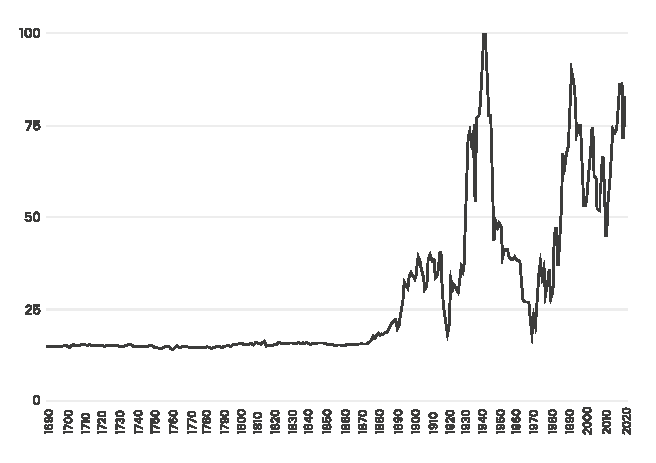
\includegraphics[width=\textwidth]{figures/fig19.pdf}
    \caption[Goud/zilver\index{zilver} verhouding]{Goud/zilver\index{zilver} verhouding}
    \label{fig19}
\end{figure}

De hoge stock-to-flow ratio van goud\index{goud} heeft ervoor gezorgd dat het een monetaire rol heeft kunnen spelen, omdat het de beste verkoopbaarheid\index{verkoopbaarheid} door de tijd heen geeft. Omdat de productie\index{productie} van goud\index{goud} slechts kleine hoeveelheden toevoegt aan de voorraad van het metaal, behoudt het zijn waarde in de loop van de tijd beter, waardoor de marktwaarde die erin is opgeslagen in de loop van de tijd toeneemt door de waardestijging ten opzichte van andere grondstoffen. Een waardestijging van tegoeden gehouden in een bepaald middel komt overeen met een toename van de liquiditeit\index{liquiditeit} van die markt, een afname van de bied-laat spread en dus een toename van de verkoopbaarheid\index{verkoopbaarheid} van de grondstof. Deze trend wordt daardoor alleen maar versterkt naarmate mensen er zich bewuster van worden en meer van hun contante geldreserves gaan aanhouden in de vorm van het goed met de hoogste verwachte toekomstige waarde en de kleinste bied-laat spread. Deze trend wordt daardoor alleen maar versterkt.

Het raamwerk van verkoopbaarheid\index{verkoopbaarheid} door tijd en de stock-to-flow ratio zijn bijzonder interessante hulpmiddelen om te gebruiken bij het analyseren van de opkomst van bitcoin\index{bitcoin}, een nieuw monetair fenomeen met een voorgeprogrammeerde aanboddynamiek en een stock-to-flow ratio die constant toeneemt tot het oneindig is. Dit analytisch kader vormt de basis van mijn eerste boek, \emph{De Bitcoin Standaard}.

\vspace{-1em}
\hypertarget{waarom-euxe9n-geldsoort}{%
\section{Waarom één geldsoort?}\label{waarom-euxe9n-geldsoort}}

Een grotere monetaire vraag\index{monetaire vraag} naar het meest verkoopbare goed zal de prijs\index{prijs} en waarde ervan verder verhogen, waardoor de verkoopbaarheid\index{verkoopbaarheid} ervan door tijd nog verder toeneemt en de liquiditeit\index{liquiditeit} ervan groeit. Aangezien rijkdom zich van nature concentreert in de meest verkoopbare goederen, zal dit de verkoopbaarheid\index{verkoopbaarheid} ervan verder vergroten. Eigenaars van de meest verkoopbare goederen zullen een grotere markt en een grotere hoeveelheid liquiditeit\index{liquiditeit} hebben waarmee ze kunnen handelen. Het toenemende gebruik als geld verhoogt de waarde van een goed als geld, waardoor de stimulans om het als geld te gebruiken toeneemt, wat resulteert in een ``winner-takes-all'' dynamiek op de geldmarkt. De geschiedenis toont aan dat dit het geval is. Aan het eind van de negentiende eeuw was de hele planeet overgeschakeld op goud\index{goud} als geld, zelfs toen duizenden verschillende goederen over de hele wereld voor deze rol werden gebruikt. Het voortbestaan van de monetaire rol van zilver\index{zilver} in de negentiende eeuw was een gevolg van de superieure verkoopbaarheid\index{verkoopbaarheid} op kleine schaal, maar toen het moderne bankieren dit overbodig maakte, werd goud\index{goud} het geld van de wereld. Iets soortgelijks gebeurt op de moderne wereldmarkt voor overheidsgeld\index{overheidsgeld}, waar er een onverzadigbare vraag lijkt te zijn naar het meest verhandelbare overheidsgeld\index{overheidsgeld}, de Amerikaanse dollar\index{Amerikaanse dollar}. Niet alleen willen heel veel niet-Amerikanen de Amerikaanse dollar\index{Amerikaanse dollar} bezitten in plaats van hun nationale valuta, vrijwel alle nationale valuta worden gedekt door dollars, omdat hun centrale banken grote hoeveelheden dollars bezitten die ze gebruiken voor de internationale handel.

Hoe algemener het ruilmiddel\index{ruilmiddel} gebruikt wordt, hoe beter het verkoopbaar is en hoe groter de potentiële markt waaraan de eigenaar kan verkopen. Individuen zullen zich van nature richten op de meest verkoopbare goederen en dat zal op zijn beurt hun verkoopbaarheid\index{verkoopbaarheid} vergroten, waardoor meer individuen worden aangetrokken om ze te gebruiken. Rothbard legde het proces als volgt uit: ``Zo gauw de meer verkoopbare goederen in een samenleving worden gekozen als ruilmiddel\index{ruilmiddel}, zullen de keuzes zich snel richten op de weinige best verkoopbare goederen die beschikbaar zijn.''\autocite{114}

Het fundamentele probleem van het samenvallen van behoeften\index{samenvallen van behoeften} betreft het samenvallen van behoeften\index{samenvallen van behoeften} naar goederen. Naarmate de omvang van een economie toeneemt, neemt ook de mate van specialisatie en het aantal goederen dat kan worden geproduceerd toe, waardoor de mogelijkheden voor directe ruilhandel\index{ruilhandel} worden bemoeilijkt. De enige mogelijke oplossing voor dit probleem, en de enige manier waarop de omvang van een markt kan groeien, is door gebruik te maken van indirecte ruil\index{indirecte ruil}, waarbij mensen goederen kopen puur om ze later te ruilen voor andere goederen. Omdat mensen verschillende goederen indirect met elkaar ruilen, is het logisch dat sommige goederen de rol van ruilmiddel\index{ruilmiddel} beter spelen dan andere, waardoor degenen die ze gebruiken worden beloond en degenen die ruilmiddelen gebruiken die ongeschikt zijn voor deze rol worden gestraft. Met het verstrijken van de tijd worden de voordelen van het gebruik van geschikte ruilmiddelen duidelijker, net als de nadelen van het gebruik van slechte ruilmiddelen. Mensen die instabiele, niet-homogene, niet-opdeelbare en niet-verplaatsbare goederen gebruiken, zullen hun rijkdom in de loop der tijd zien afnemen, terwijl mensen die stabiele, homogene, zeer deelbare en verplaatsbare goederen gebruiken, hun rijkdom zullen zien toenemen. Naarmate de tijd verstrijkt, worden primitieve en ongeschikte monetaire middelen afgedankt en genegeerd terwijl hun gebruikers hun rijkdom verliezen, en op de lange termijn wordt het belangrijkste meetinstrument bij het bepalen van de monetaire status de maatstaf van hardheid, of stock-to-flow ratio.

Het proces van monetaire concurrentie wordt zowel aangejaagd door menselijk handelen\index{menselijk handelen} als door de brute fysieke, chemische en geologische realiteit die de productie\index{productie} van verschillende goederen bepaalt. Intelligente mensen zullen hun verstand gebruiken om de beste vorm van geld te vinden, maar zelfs als niemand hieraan zou denken, zou de economische realiteit zichzelf opdringen en een vergelijkbaar resultaat opleveren. Degenen die het beste geld gebruiken zullen meer rijkdom vergaren, terwijl degenen die ongeschikt geld gebruiken hun rijkdom zullen verliezen, en na verloop van tijd zal het meerendeel van de welvaart geconcentreerd zijn bij degenen die het beste geld gebruiken, of ze dit resultaat nu bewust voor ogen hadden of niet.

De bovenstaande analyse verklaart het ontstaan van geld op basis van het vermogen om de essentiële functie van geld te vervullen: fungeren als ruilmiddel\index{ruilmiddel}. Rothbard definieerde geld als een goed dat algemeen gebruikt wordt als ruilmiddel\index{ruilmiddel}. Terwijl het concept van een ruilmiddel\index{ruilmiddel} concreet is, is het concept van een ``algemeen ruilmiddel\index{ruilmiddel}'' dat niet. Het is gemakkelijk om iets te identificeren dat functioneert als een ruilmiddel\index{ruilmiddel}, maar het identificeren als een \textit{algemeen} ruilmiddel\index{ruilmiddel} is een kwestie van subjectief oordeel.

\hypertarget{geld-en-de-staat}{%
\section{Geld en de staat}\label{geld-en-de-staat}}

De Oostenrijkse benadering van economie als de studie van menselijk handelen\index{menselijk handelen} kan ons helpen om te begrijpen en te identificeren welke goederen waarschijnlijk een monetaire rol zullen spelen, simpelweg door de manier te analyseren waarop mensen handelen bij het oplossen van problemen rondom ruilhandel\index{ruilhandel}. Zelfs voordat mensen hun handelingen konden vastleggen, deden ze al aan directe en indirecte ruil\index{indirecte ruil}. En omdat mensen hun behoeften proberen te vervullen door middel van indirecte ruil\index{indirecte ruil}, beginnen sommige goederen die rol beter te spelen dan andere, en degenen die dit goed gebruiken profiteren. Andere mensen volgen dit voorbeeld en de succesvolle oplossingen raken wijder verspreid. Degenen die succesvolle oplossingen niet kopiëren, verliezen rijkdom aan degenen die dat wel doen. De betere oplossingen dringen zichzelf op zoals de economische realiteit dat altijd doet, door degenen die ze toepassen te belonen en degenen die dat niet doen te straffen. Er is geen centrale autoriteit nodig om een ruilmiddel\index{ruilmiddel} voor te schrijven en iedereen te dwingen het te accepteren. Geld ontstaat uit de markt, uit de handelingen van mensen, en niet als resultaat van een centraal plannende overheid\index{overheid}.

Zoals Carl Menger\index{Carl Menger} uiteenzette: ``Geld is geen uitvinding van de staat. Het is niet het product van een wetgevende handeling. De goedkeuring van een politieke autoriteit is niet noodzakelijk voor het bestaan ervan. Bepaalde goederen werden op een heel natuurlijke manier geld, als het resultaat van economische relaties die onafhankelijk waren van de macht van de staat.''\autocite{115} Bepaalde goederen zullen van nature beter beter geschikt zijn als geld dan andere, en het marktproces zal deze naar voren brengen en ervoor zorgen dat ze steeds meer als geld worden gebruikt. Dit proces is vergelijkbaar met de selectie van bepaalde grondstoffen voor de productie\index{productie} van een consumptiegoed\index{consumptiegoed}: zoals leer wordt gebruikt voor schoenen, benzine voor de aandrijving van auto\textquotesingle s en silicium voor elektronica, resulteert het marktproces in de selectie van de meest verkoopbare goederen als geld.

Mises ging verder dan Menger door uit te leggen hoe de keuze voor geld puur op de markt kan ontstaan door middel van zijn \textbf{regressie-theorema}, dat uitlegde hoe een normaal marktgoed zich kan ontwikkelen tot een monetair goed wanneer er monetaire vraag\index{monetaire vraag} naar ontstaat, waardoor de waarde stijgt en de verkoopbaarheid\index{verkoopbaarheid} toeneemt. Naarmate de monetaire vraag\index{monetaire vraag} naar het goed toeneemt, stijgt de prijs\index{prijs} ervan tot boven de marktvraagprijs.

Het proces van monetaire ontwikkeling en marktselectie is volledig te begrijpen vanuit het oogpunt van menselijk handelen\index{menselijk handelen}. Er is geen enkele dwingende autoriteit nodig om een monetair middel te selecteren of te produceren. Geld komt, net als alle andere goederen, op de markt omdat het een nut heeft waardoor individuen er waarde aan hechten. De historische en empirische gegevens ondersteunen deze stelling, omdat ze duidelijk laten zien dat monetaire middelen dateren van vóór de monetaire mandaten van de overheid\index{overheid}. De wereldwijde monetaire rol van goud\index{goud} werd niet toegekend door een of andere overheidsinstantie. Het won zijn monetaire rol op de markt, en overheden moesten goud\index{goud} als geld op de markt accepteren als ze succesvol wilden opereren. Goud werd geen geld omdat het in overheidsmunten werd geslagen. Overheidsmunten werden geld omdat ze uit goud\index{goud} werden geslagen.

De geschiedenis laat geen enkel voorbeeld zien van een goed of activum dat zijn monetaire rol kreeg door een mandaat van de overheid\index{overheid}. Modern overheidsgeld\index{overheidsgeld} wordt fiatgeld\index{fiatgeld} genoemd, gebaseerd op het Latijnse woord fiat\index{fiat}, dat een decreet van een autoriteit betekent. Toch is het niet als fiatgeld\index{fiatgeld} in omloop gebracht. Al het bestaande overheidsgeld\index{overheidsgeld} kreeg zijn monetaire rol oorspronkelijk door de keuze van de vrije markt voor geld, namelijk goud\index{goud}. Alleen door hun monetaire beleid aan te passen aan de keuze van de markt kon ``fiatgeld\index{fiatgeld}'' van de overheid\index{overheid} überhaupt geaccepteerd worden als geld. Alleen door op frauduleuze wijze de inwisseling van dit overheidsgeld\index{overheidsgeld} voor goud\index{goud} te herroepen ontstond ``fiatgeld\index{fiatgeld}'', niet door pure fiat\index{fiat}. Het uiteindelijke verbreken van de inwisselbaarheid met goud\index{goud} verandert niets aan het feit dat geen enkel geld ooit zijn monetaire rol heeft gekregen door fiat\index{fiat}. Verder illustreert de voortdurende behoefte van regeringen om monopolies op te leggen op het gebied van bankieren en wettige betaalmiddelen, dat hun opdringen van geld de concurrentie van de vrije markt niet kan overleven. Regeringen konden de monetaire waarde van goud\index{goud} niet opleggen; ze namen het met geweld in beslag en accumuleerden het. Nog steeds, meer dan een eeuw na het einde van de goudstandaard\index{goudstandaard}, blijven de centrale banken van de wereld steeds grotere hoeveelheden goud\index{goud} accumuleren.

Een ander krachtig argument tegen de overheidstheorieën over geld komt van de opkomst van bitcoin\index{bitcoin}, dat in de afgelopen 14 jaar is uitgegroeid vanuit het niets tot een van de 20 belangrijkste valuta ter wereld, allemaal zonder dat een enkele wettelijke autoriteit het gebruik ervan heeft gepromoot of voorgeschreven. El Salvador kondigde bitcoin\index{bitcoin} aan als wettig betaalmiddel in 2021, maar dat kwam pas nadat bitcoin\index{bitcoin} al was uitgegroeid tot een van de 20 belangrijkste valuta ter wereld op basis van marktkapitalisatie. Net als met goud\index{goud}, zilver\index{zilver} en alle andere vormen van geld, volgt de erkenning van de staat de economische realiteit; ze gaat er niet aan vooraf of dicteert ze niet. Als geld een uitvinding van de staat was geweest, en overheidssubsidie nodig had gehad om te functioneren, dan had bitcoin\index{bitcoin} niet zo succesvol kunnen zijn als nu het geval is.

\hypertarget{waarde-van-geld}{%
\section{Waarde van geld}\label{waarde-van-geld}}

Net als eerdere methoden van economisch\index{economisch} handelen, is geld ook een middel om de hoeveelheid en de waarde van onze tijd op aarde te vergroten. De introductie van geld in een economie versterkt alle drie de drijvende krachten achter economische groei en vooruitgang. We kunnen de economische betekenis van geld beter begrijpen aan de hand van de drie hoofdfuncties die het vervult: ruilmiddel\index{ruilmiddel}, spaarmiddel\index{spaarmiddel} en rekeneenheid\index{rekeneenheid}.

\subsection{1. Vergroot de arbeidsdeling\index{arbeidsdeling}}

Omdat geld het probleem van het samenvallen van behoeften\index{samenvallen van behoeften} elimineert, maakt het uitgebreide handel mogelijk tussen vreemden die elkaar niet hoeven te vertrouwen of deel hoeven uit te maken van politieke en economische structuren die hen beschermen. Het bestaan van geld op de markt vergroot de ruimte voor \textbf{specialisatie en arbeidsdeling\index{arbeidsdeling}}, waardoor de markt voor elke consument en elk product enorm wordt verbreed. Hoe effectiever een monetair middel is in het behouden van zijn waarde over afstand, en hoe meer het in het bezit is van anderen, hoe meer handelsmogelijkheden het biedt aan de bezitters en hoe groter de omvang van de markt. Naarmate individuen zich realiseren dat ze in steeds meer van hun behoeften kunnen voorzien door goederen met anderen te ruilen, zullen ze eerder geneigd zijn samenwerking en vrede te zoeken met vreemden met wie ze nooit twee keer in contact zullen komen. Met geld vinden menselijke arbeid, kapitaalaccumulatie, technologische innovaties en handel plaats binnen in een groot uitgebreid systeem van onpersoonlijke ruil\index{ruil}. Mensen die elkaar niet kennen en die niet direct met elkaar samenwerken, slagen er toch in om via complexe productiestructuren zeer geavanceerde producten te maken. Geld is een essentieel instrument voor de menselijke beschaving\index{beschaving} en de vernietiging ervan is altijd samengevallen met de vernietiging van de samenleving en het beschaafde leven.

\subsection{2. Economische berekeningen mogelijk maken}

Een belangrijke implicatie van het gebruik van geld is dat alle prijzen worden uitgedrukt in één eenheid. In een economie met geld is geld de helft van elke transactie. Een ruilhandeleconomie met 10 goederen zou 45 verschillende prijzen vereisen, die elk een goed uitdrukken in relatie tot een ander goed (aantal individuele prijzen = n(n-1)/2, waarbij n=aantal goederen). Een geldeconomie met 10 goederen (inclusief het monetaire goed) zou daarentegen slechts 9 prijzen nodig hebben (aantal individuele prijzen = n-1). Het aantal prijzen in een ruilhandeleconomie neemt exponentieel toe met het aantal goederen, terwijl de relatie tussen het aantal prijzen en goederen in een geldeconomie lineair is. We kunnen zien dat voor een ruileconomie met 100 goederen maar liefst 4.950 verschillende prijzen nodig zijn, terwijl voor een geldeconomie met 100 goederen slechts 99 prijzen nodig zijn. Een ruileconomie met 1.000.000 goederen zou bijna 500 miljard verschillende prijzen vereisen, maar een geldeconomie met 1.000.000 goederen zou slechts ~999.999~ prijzen vereisen. De introductie van geld in een economie vermindert dus drastisch het aantal prijzen dat nodig is voor handel, waardoor handel en markten\index{markten} buitengewoon efficiënt worden.

Het uitdrukken van de prijs\index{prijs} van alle goederen in één ander goed laat ons toe economische berekeningen uit te voeren, wat het onderwerp zal zijn van Hoofdstuk 12. Met alle prijzen in één eenheid is de ondernemer in staat om zorgvuldig de verwachte kosten en opbrengsten van een onderneming te berekenen. Met berekeningen met de gemeenschappelijke noemer geld, kunnen individuen ``een steeds groter en langer geheel van productiefasen construeren om tot de gewenste goederen te komen, omdat geld verfijnde berekeningen mogelijk maakt'', zoals Rothbard het formuleerde.\autocite{116}

De specialisatiegraad in de moderne wereldeconomie is alleen mogelijk door het gebruik van geld. Individuen kunnen goederen produceren zonder zich zorgen te hoeven maken over om hun eigen consumptie\index{consumptie} van die goederen, omdat ze weten dat ze die op de markt kunnen inruilen voor het meest verkoopbare goed, dat ze vervolgens weer kunnen inruilen voor welk ander goed ze maar willen. Complexe productieprocessen en lange productieketens zijn alleen mogelijk dankzij de specialisatie die geld mogelijk maakt.

\subsection{3. Lagere tijdsvoorkeur}

Geld stelt, als middel voor het uitwisselen van waarde, eigenaars in staat om waarde op een efficiëntere manier te behouden en over te dragen naar de toekomst dan anders het geval zou zijn. Geld heeft, zoals hierboven uitgelegd, een hogere verkoopbaarheid\index{verkoopbaarheid} dan andere marktgoederen en zal van nature evolueren tot een goed met een hoge verkoopbaarheid\index{verkoopbaarheid} door tijd; het zal daardoor beter zijn waarde behouden  dan de meeste andere marktgoederen. Naarmate geld beter verkoopbaar is, kan het beter in de toekomst voorzien, wat de onzekerheid over de toekomst vermindert, en leidt tot een afname van de discontering van de toekomst. Dit is eenvoudigweg het verlagen van de tijdsvoorkeur\index{tijdsvoorkeur}, zoals wordt besproken in Hoofdstuk 3 en 13.

Geld kan dus worden opgevat als een belangrijke technologie voor het verlagen van de menselijke tijdsvoorkeur\index{tijdsvoorkeur}, omdat het een uiterst krachtig middel is om in de toekomst te voorzien, de onzekerheid daaromheen te verminderen en de eigenaars ervan in staat te stellen die toekomst te plannen. Het afdekken van onzekerheid is een van de belangrijkste functies van geld, en het is de reden waarom mensen liever wat geld aanhouden dan alleen kapitaalgoederen\index{kapitaalgoederen}, ook al leveren die laatste een rendement op en de eerste niet.\autocite{117} Investeringen zijn minder goed verkoopbaar en brengen ondernemersrisico met zich mee. Geld is in een vrije markt het goed met de meeste verkoopbaarheid\index{verkoopbaarheid} en het minste risico\index{risico}; het is het goed dat altijd kan worden omgezet in andere goederen met het kleinste verlies van zijn economische waarde. Geld mag dan geen rendement opleveren, het wordt nog steeds aangehouden omdat het van alle activa het minst onzeker is.\autocite{118} Tijdsvoorkeur is een maatstaf voor het waarderen van de toekomst, en onzekerheid heeft een grote invloed op hoeveel waarde we eraan hechten. Het beschikken over geld, en in het bijzonder goed en hard geld\index{hard geld}, is een manier om deze onzekerheid te verminderen.

\clearpage
Hans-Hermann Hoppe\index{Hans-Hermann Hoppe} stelde dat het beschavingproces begint bij het verlagen van de tijdsvoorkeur\index{tijdsvoorkeur}.\autocite{119} Geld is daarin cruciaal. Hoe harder het geld is, hoe beter het zijn waarde voor de toekomst kan behouden en hoe minder onzeker de toekomst zal zijn. Hoe meer mensen hun toekomst kunnen plannen en op de lange termijn kunnen gedijen, hoe meer geld ervoor zal zorgen dat de tijdsvoorkeur\index{tijdsvoorkeur} afneemt en de beschaving\index{beschaving} gedijt.
\hypertarget{de-uniekheid-van-geld}{%
\section{De uniciteit van geld}\label{de-uniekheid-van-geld}}

Geld als goed onderscheidt zich op verschillende manieren van andere goederen. Het eerste onderscheid is dat geld noch een consumptiegoed\index{consumptiegoed} noch een kapitaalgoed\index{kapitaalgoederen} is. Consumptiegoederen worden aangeschaft om geconsumeerd te worden omdat ze rechtstreeks menselijke behoeften dienen te voldoen. Kapitaalgoederen daarentegen voorzien niet direct in menselijke behoeften, maar worden aangeschaft omdat ze kunnen worden gebruikt om goederen te produceren die in menselijke behoeften voorzien. Geld is echter geen van beide. Het wordt niet gekocht omdat het menselijke behoeften vervult, noch kan het worden gebruikt voor de productie\index{productie} van andere goederen; het wordt puur gekocht om in de toekomst te worden geruild voor andere goederen, of dat nu consumptiegoederen\index{consumptiegoed} of kapitaalgoederen\index{kapitaalgoederen} zijn.

Het gebruik als ruilmiddel\index{ruilmiddel} is de essentiële functie van geld, en dit betekent dat het geen direct nut nodig heeft voor mensen om het te waarderen. Het nut van geld wordt afgeleid van het nut van de goederen waarvoor het kan worden geruild. Geld zal, net als alle goederen, een afnemend marginaal nut\index{marginaal nut} hebben, maar het marginale nut neemt minder snel af dan het marginale nut van alle andere goederen, omdat elke volgende geldeenheid kan worden gebruikt om een eenheid te kopen van de volgende meest waardevolle eenheid van een goed, en niet alleen de volgende meest waardevolle eenheid van hetzelfde goed. Bijvoorbeeld, in een economie met geld en slechts drie goederen, bijvoorbeeld bananen, appels en sinaasappels, zal het nut van geld minder afnemen dan het nut van elke appel, sinaasappel en banaan afzonderlijk. Aangezien geld liquide is en eenvoudig kan worden ingewisseld voor andere goederen, is het handiger om het aan te houden dan andere goederen. Deze verkoopbaarheid\index{verkoopbaarheid} is de reden waarom mensen liever in geld worden betaald dan in voorwerpen met een beperkte verkoopbaarheid\index{verkoopbaarheid}. De hoge verkoopbaarheid\index{verkoopbaarheid} geeft geld het nut van het goed dat op dat moment toevallig het meest waardevol is voor de eigenaar van het geld.

\vspace{-0.5em}
\hypertarget{hoeveel-geld-moet-er-zijn}{%
\section{Hoeveel geld moet er zijn?}\label{hoeveel-geld-moet-er-zijn}}

Misschien wel het belangrijkste monetaire onderscheid tussen mainstream economen en Oostenrijkse economen is dat Oostenrijkers de absolute geldhoeveelheid onbelangrijk vinden en dat de geldhoeveelheid dus niet hoeft te groeien om te voldoen aan de behoeften van een groeiende economie. Elke geldhoeveelheid is voldoende voor elke economie, zolang het maar voldoende deelbaar is. Geld is onder economische goederen uniek, omdat het het enige goed is waarvan de absolute hoeveelheid er niet toe doet voor de eigenaar. Geld biedt de eigenaar geen andere diensten dan de mogelijkheid om het te ruilen voor andere goederen, waardoor de absolute hoeveelheid die de eigenaar bezit irrelevant is. Het enige aspect van geld dat er voor de eigenaar toe doet, is de koopkracht ervan. De economische waarde van geld ligt in het vermogen om het te ruilen voor andere goederen, en dus komt de waarde van geld voort uit zijn koopkracht, niet uit zijn hoeveelheid. Elke geldhoeveelheid kan voldoende zijn voor elke economie, mits het kan worden opgedeeld in kleine eenheden. Rothbard legt het als volgt uit:

\begin{blockquotebox}
    Geld verschilt in minstens één essentieel opzicht fundamenteel van consumptiegoederen\index{consumptiegoed} en productiegoederen. De toename van het aanbod van consumptiegoederen\index{consumptiegoed} is goed voor de samenleving, omdat een of meer consumenten beter af zullen zijn. Hetzelfde geldt voor een toename in het aanbod van productiegoederen, die uiteindelijk zullen worden omgezet in een groter aanbod van consumentengoederen; want productie\index{productie} zelf is het proces waarbij natuurlijke grondstoffen worden omgezet in nieuwe vormen en locaties, in overeenstemming met de wensen van consumenten voor direct gebruik. Geld is echter heel anders: geld wordt niet direct gebruikt voor consumptie\index{consumptie} of productie\index{productie}, maar het wordt geruild voor zulke direct te gebruiken goederen. Maar als een goed of voorwerp eenmaal geld is, heeft het de maximale ruilcapaciteit. Een toename van de geldhoeveelheid levert geen enkele verbetering op in de ruilfunctie van geld; het enige dat gebeurt, is dat de koopkracht van elke geldeenheid verwatert door het toegenomen aantal eenheden. Er is dus nooit een sociale noodzaak om de geldhoeveelheid te vergroten, niet vanwege een toegenomen aanbod van goederen, noch vanwege een toename van de bevolking. Mensen kunnen hun deel van de geldhoeveelheid vergroten door minder uit te geven en zo de koopkracht van hun kassaldo te verhogen, wat zal leiden tot een toename van hun totale reële kassaldo.\footnotemark
\end{blockquotebox}
\footautocite{120}

Rothbard citeert vervolgens Mises:

\begin{blockquotebox}
    De diensten die geld levert, worden bepaald door de koopkracht ervan. Niemand wil een bepaalde geldhoeveelheid of een specifiek gewicht aan geld in zijn kas hebben; men wil een hoeveelheid koopkracht bezitten. Aangezien de marktwerking de uiteindelijke koopkracht van geld bepaalt op een hoogte waarop het aanbod van en de vraag naar geld samenvallen, kan er nooit een overschot of een tekort aan geld zijn. Elk individu en alle individuen samen genieten altijd ten volle van de voordelen die ze kunnen halen uit indirecte ruil\index{indirecte ruil} en het gebruik van geld, ongeacht of de totale hoeveelheid geld groot of klein is. Veranderingen in de koopkracht van geld veroorzaken veranderingen in de verdeling van rijkdom onder de verschillende leden van de maatschappij. Vanuit het oogpunt van mensen die graag rijker willen worden door dergelijke veranderingen, kan de geldhoeveelheid ontoereikend of juist buitensporig worden genoemd, en de zucht naar dergelijke winsten kan leiden tot beleid dat de koopkracht probeert te veranderen aan de hand van aanpassingen van de geldhoeveelheid. De diensten die geld levert, kunnen echter niet worden verbeterd of hersteld door de geldhoeveelheid te veranderen. Er kan een overschot of een tekort aan geld zijn in de geldvoorraad van een individu. Maar zo\textquotesingle n toestand kan worden verholpen door de consumptie\index{consumptie} of investeringen te verhogen of te verlagen. (Natuurlijk moet men niet ten prooi vallen aan de populaire verwarring tussen de vraag naar geld voor het aanhouden van contant geld\index{contant geld} en het verlangen naar meer rijkdom). De geldhoeveelheid die in de hele economie beschikbaar is, is altijd voldoende om iedereen te verzekeren van alles wat geld te beiden heeft.\footnotemark
\end{blockquotebox}
\footautocite{121}    

Rothbard voegt hieraan toe:

\begin{blockquotebox}
    Een wereld met een constante geldhoeveelheid zou vergelijkbaar zijn met die van een groot deel van de achttiende en negentiende eeuw, gekenmerkt door de succesvolle bloei van de industriële revolutie met toegenomen kapitaalinvesteringen die het aanbod van goederen deden toenemen, met dalende prijzen voor die goederen, en ook dalende productiekosten.\footnotemark
\end{blockquotebox}
\footautocite{122}

\clearpage
Volgens de Oostenrijkse visie zal, als de geldhoeveelheid vastligt, de economische groei de reële prijzen van goederen en diensten doen dalen, waardoor mensen in de toekomst steeds meer goederen en diensten met hun geld kunnen kopen. Zo\textquotesingle n wereld zou inderdaad directe consumptie\index{consumptie} ontmoedigen, precies zoals de Keynesianen vrezen, maar wanneer er meer geconsumeerd kan worden, zou het ook sparen en investeren voor de toekomst, aanmoedigen. Omdat Keynesiaanse economen weinig begrip tonen van het concept van kapitaal\index{kapitaal} en marginale analyse, zien ze een daling van de consumptie\index{consumptie} als een ramp. Als de totale bestedingen afnemen in Keynesiaanse economische modellen met een hoge tijdsvoorkeur\index{tijdsvoorkeur}, zullen werknemers ontslagen worden, wat op zijn beurt zal leiden tot nog minder uitgaven, wat weer leidt tot meer ontslagen en een voortdurende neerwaartse spiraal die eindigt in armoede. Volgens de Keynesianen kunnen alleen actieve centrale overheden die rijkelijk geld uitgeven deze nachtmerrie voorkomen.

Maar voor niet-Keynesianen -- oftewel economen die bekend zijn met het concept van kapitaal\index{kapitaal} -- is een daling van de uitgaven niet alleen ongevaarlijk, het is de basis van de beschaafde samenleving. Alleen door minder te consumeren en meer te sparen, is kapitaalinvestering mogelijk, zoals besproken in Hoofdstuk 6. Voor economen die bekend zijn met marginale analyse, zal een afname in de neiging om geld uit te geven leiden tot een afname van de marginale uitgaven, en niet tot een volledige stopzetting van de consumptie\index{consumptie}. Zoals besproken in Hoofdstuk 3 is tijdsvoorkeur\index{tijdsvoorkeur} positief, en individuen geven altijd de voorkeur aan consumptie\index{consumptie} in het heden boven consumptie\index{consumptie} in de toekomst. Consumptie in het heden is noodzakelijk om te overleven. Individuen hoeven de waarde van hun geld niet te zien verdampen om te gaan consumeren; de natuur dwingt hen om te consumeren om te overleven. Naarmate sparen voor de toekomst veiliger wordt, kunnen ze hun consumptie\index{consumptie} marginaal verminderen, maar ze kunnen niet volledig afzien van consumptie\index{consumptie}. Deze marginale vermindering van de consumptie\index{consumptie} kan leiden tot een afname van de marginale werkgelegenheid in de productie\index{productie} van consumptiegoederen\index{consumptiegoed}, maar niet tot een volledige ineenstorting van de werkgelegenheid. Anderzijds maakt de verminderde
consumptie\index{consumptie} middelen vrij die niet langer als consumptiegoederen\index{consumptiegoed} worden gebruikt, maar kunnen worden ingezet als kapitaalgoederen\index{kapitaalgoederen}. Geld sparen komt overeen met het besparen op economische middelen voor consumptie\index{consumptie}. Hierdoor zijn er meer mogelijkheden om werk te maken van eerdere fasen van economische productie\index{productie}. Hierdoor ontstaan er meer mogelijkheden om werk te richten op de eerdere fasen van de economische productie\index{productie}. Een samenleving die consumptie\index{consumptie} voortdurend uitstelt, zal uiteindelijk meer consumeren dan een samenleving met weinig spaargeld, omdat de samenleving met een lage tijdsvoorkeur\index{lage tijdsvoorkeur} meer investeert en zo meer inkomen produceert voor haar leden. Ook al gaat een groter percentage van hun inkomen naar sparen, samenlevingen met een lage tijdsvoorkeur\index{lage tijdsvoorkeur} zullen op langere termijn hogere consumptieniveaus hebben, evenals een grotere kapitaalvoorraad. In plaats van armoede te veroorzaken, is de vermindering van consumptie\index{consumptie} de enige weg naar overvloed.

\hypertarget{markten}{%
\chapter{Markten}\label{markten}}

\vspace{-2em}
\begin{blockquotebox}
    In een markteconomie, een sociaal systeem gebaseerd op arbeidsdeling\index{arbeidsdeling} en privaat eigendom van productiemiddelen, handelt iedereen uit eigenbelang. Dit eigenbelang dient echter tegelijkertijd de behoeften van anderen. Zo dient ieders handelen zijn medemens, terwijl hij ook door anderen gediend wordt. In dit systeem fungeert iedereen zowel als middel voor de doelen van anderen, als ook als een doel op zichzelf, strevend naar persoonlijke doelstellingen.
\footnotemark
    \par\raggedleft--- Ludwig von Mises\index{Ludwig von Mises}
\end{blockquotebox}
\footautocite{123}

Geld maakt specialisatie en arbeidsdeling\index{arbeidsdeling} mogelijk, wat het ontstaan en de groei van een markteconomie bevordert. \textbf{Een markteconomie is een sociale orde waarin mensen in staat zijn om in zeer grote aantallen samen te werken aan economische productie\index{productie}, waarbij ze elkaar vrijwillig goederen en diensten leveren voor alle betrokkenen, zonder dat een dwingende autoriteit hun handelen dicteert en coördineert.}

Om de enorme voordelen van een markteconomie te waarderen, is het goed je de impact op je leven, overlevingskansen en de kwantiteit en kwaliteit van je tijd voor te stellen wanneer je afgezonderd van de wereld of in een kleine stam zou leven, zonder ruilhandel\index{ruilhandel} met de rest van de wereld. Het aanbod van goederen zou heel klein zijn en de mogelijkheden om jezelf tegen de natuur te beschermen zouden heel beperkt zijn. Je specialiseren in bijvoorbeeld lassen of schilderen zou onmogelijk zijn, omdat je al je uren zou besteden aan het de meest basale taken die nodig zijn om niet te verhongeren of dood te vriezen. De mens wil deelnemen aan de markteconomie vanwege dwingende en ongeëvenaarde voordelen die het de deelnemers biedt, in tegenstelling tot de uitzichtloze alternatieven.

In een markteconomie hoeven individuen niet na te denken over hun eigen productie\index{productie} voor hun eigen consumptiebehoeften. Door de toenemende specialisatie en arbeidsdeling\index{arbeidsdeling} kan elk individu zich richten op de productiemethoden die hem in geld uitgedrukt de beste beloning voor zijn inspanning bieden, waardoor hij de goederen die hij voor zijn eigen behoeften aanschaft kan maximaliseren. In plaats van voor zichzelf de goederen te produceren die hij nodig heeft, specialiseert een deelnemer aan de markteconomie zich in het leveren van de goederen die hij het beste kan produceren voor anderen, en is hij afhankelijk van andere mensen voor het verkrijgen van de goederen die hij zelf nodig heeft. Uiteindelijk zorgt het kapitalistische marktsysteem ervoor dat mensen zich specialiseren in wat ze het beste kunnen en zich richten op hoe ze anderen waarde kunnen bieden, in plaats van zich te richten op wat ze zelf belangrijk vinden. Mensen kiezen in een kapitalistisch systeem om anderen te dienen, omdat het veel productiever en efficiënter is dan alleen voor jezelf, losstaand van de arbeidsdeling\index{arbeidsdeling}, te werken.

Het wonder van de markteconomie, dat vaak onderschat wordt, is de manier waarop het samenwerking tussen mensen mogelijk maakt zonder dwang, centrale regie of sociale verplichtingen. Wat de activiteiten van producenten binnen de arbeidsdeling\index{arbeidsdeling} coördineert, is hun vermogen om economische berekeningen uit te voeren over het optimale gebruik van hun middelen. Dit doen ze met behulp van een gemeenschappelijke maatstaf, namelijk de monetaire prijs, oftewel de prijs\index{prijs} uitgedrukt in geld. Naarmate een economie groeit tot een niveau waarop alle economische goederen op een markt kunnen worden gekocht en verkocht in ruil\index{ruil} voor één ander goed, kunnen deelnemers aan de economie de verschillende kosten en baten van elke handelswijze berekenen en vergelijken met hun eigen voorkeuren en met de beschikbare alternatieven. De vrijheid die iedereen heeft om zijn voorkeuren uit te drukken door middel van economisch\index{economisch} handelen, geeft iedereen de zelfzuchtige prikkel om te handelen op een manier die aan de behoeften van anderen voldoet. Het is geen autoriteit of geweld dat het handelen van mensen bepaalt, maar hun verlangen om aan hun eigen behoeften te voldoen, volgens de berekeningen die ze uitvoeren op basis van prijzen die de voorkeuren van andere deelnemers aan de markt uitdrukken. Zoals Mises het stelde:

\clearpage

\begin{blockquotebox}
    Markthandel en monetaire calculatie zijn onlosmakelijk met elkaar verbonden. Een markt waarin alleen directe ruilhandel\index{ruilhandel} plaatsvindt, is slechts een denkbeeldig idee. Aan de andere kant worden geld en monetaire calculatie bepaald door het bestaan van de markt.\footnotemark 
\end{blockquotebox}
\footautocite{124}

Wanneer de marktprijs van alle goederen wordt gemeten ten opzichte van één goed, kunnen we individuele prijzen vergelijken, zowel met andere prijzen als met hun eigen subjectieve waarderingen, en vervolgens consumptie\index{consumptie}- en productiebeslissingen nemen. Zoals al besproken in het eerste hoofdstuk van het boek, is waarde subjectief. Het kan niet objectief gemeten worden, omdat er geen constante eenheid bestaat waartegen het gemeten kan worden. Maar wanneer een individu op een markt zijn eigen keuzes maakt, weegt hij economische keuzes af tegen zijn subjectieve waarderingen. De waarden zijn misschien niet meetbaar met een constante eenheid, maar ze zijn wel vergelijkbaar met één constant referentiekader: het individu dat de waardering maakt. Door zijn eigen voorkeuren te kennen, kan de mens de verschillende voorkeuren ordenen. Hoewel we geen kardinale, numerieke waarderingen kunnen toekennen aan verschillende opties, kunnen we ze wel rangschikken op basis van onze eigen voorkeur. In dit hoofdstuk wordt een wiskundig grafisch model uitgewerkt om na te denken over hoe deze beslissingen worden genomen in de context van een markteconomie.

\vspace{-1em}
\hypertarget{markten-voor-consumentengoederen}{%
\section{Markten voor consumentengoederen}\label{markten-voor-consumentengoederen}}


Deelnemers aan een economie kopen consumptiegoederen\index{consumptiegoed} om aan hun behoeften en wensen te voldoen en ze betalen er een prijs\index{prijs} in geld voor. Individuen voeren economische berekeningen uit om de marktprijs van goederen af te wegen tegen de waardering die ze persoonlijk aan deze goederen geven. Als de prijzen veranderen, verandert natuurlijk ook de hoeveelheid van een goed dat ze kopen. Waardering is subjectief en ordinaal, niet kardinaal. Met andere woorden, individuen waarderen goederen door ze te rangschikken ten opzichte van andere goederen. Mensen hechten geen numerieke waarde aan objecten, maar vergelijken hun nut en rangschikken ze naar eigen voorkeur, zoals blijkt uit de marktkeuzes die ze maken.

We kunnen deze economische keuze zien als iets dat bereikt wordt door individuen die een waardeschaal maken: een rangorde van goederen naar individuele voorkeur. Voor elk goed weerspiegelt de waardeschaal dus de waardering van bepaalde hoeveelheden van het goed in vergelijking met monetaire eenheden.

Neem bijvoorbeeld een man die nadenkt over zijn dagelijkse behoefte aan rundvlees. Het eerste pond rundvlees van de dag, is voor hem extreem waardevol. Hij is bereid om een aanzienlijke prijs\index{prijs} te betalen om er zeker van te zijn dat hij het kan krijgen, om niet ondervoed en hongerig te zijn. Zijn inkomen, rijkdom en voorkeuren voor rundvlees in acht nemende, is hij niet bereid om \$31 betalen voor een pond rundvlees. Maar hij is wel bereid om \$30 te betalen voor het eerste pond rundvlees van de dag, wat betekent dat hij meer waarde hecht aan het eerste pond rundvlees dan aan \$30. Zodra hij dat pond heeft gekocht, wordt het tweede pond rundvlees hem iets minder waard en het overgebleven geld wordt waardevoller, omdat het minder is geworden door al voor één pond te betalen. Op dat moment is hij bereid om tot \$16 te betalen voor het tweede pond rundvlees, omdat hij het iets meer waardeert dan dit bedrag. Bij de overweging om een derde pond rundvlees te kopen, zou hij de kosten alleen dragen als de prijs \$12 of minder is. En het vierde pond zou hij alleen kopen als de prijs \$8 of lager is. Als de prijs daalt, vraagt hij meer stukken vlees, en bij een gangbare marktprijs van \$4 zou hij zijn vijfde pond rundvlees per dag consumeren. Als de prijs van rundvlees \$2 is, consumeert hij 6 pond op een dag. Bij een prijs van \$1 consumeert hij 7 pond per dag. Bij een prijs van \$0, in een wereld waarin hem gratis onbeperkt rundvlees wordt aangeboden, consumeert de man acht pond rundvlees per dag.

Op basis van deze subjectieve beslissingen kan de man zijn waardering voor verschillende hoeveelheden rundvlees en dollars rangschikken:

\begin{figure}[H]
\centering
    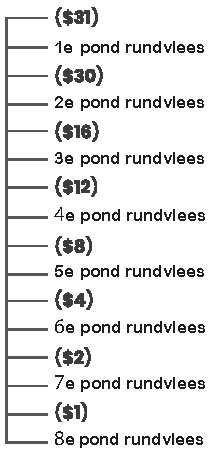
\includegraphics[height=7cm]{figures/fig20.pdf}
    \caption[Ordinale waardeschaal van consument]{Ordinale waardeschaal van consument}
    \label{fig19}
\end{figure}

De ordinale rangorde van goederen is een conceptueel hulpmiddel dat economen gebruiken om het denkproces te begrijpen dat gepaard gaat met het nemen van aankoopbeslissingen. De ordinale waardeschaal kan worden gezien als de onbewuste basis van die keuze, maar in de echte wereld wordt de koper slechts geconfronteerd met één prijs\index{prijs} en beslist hij welke hoeveelheid hij tegen die prijs\index{prijs} zal kopen. We kunnen de hoeveelheden afleiden die hij voor elke prijs\index{prijs} zou kopen. Uit deze ordinale rangschikking van rundvlees ten opzichte van monetaire eenheden, verkrijgen we een \textbf{vraagschema}: \textbf{een tabel die de gewenste hoeveelheid weergeeft bij elk prijsniveau.}

\begin{table}[!htb]
\centering
\begin{tabular}{|c|c|}  % Add vertical lines
\hline  % Top horizontal line
    \cellcolor{gray!25}Marktprijs (USD) &
    \cellcolor{gray!25}Gevraagde hoeveelheid rundvlees (pond)\\
\hline  % Horizontal line after the header
 %
 \$31 & 0 \\ \hline
 \$30 & 1 \\ \hline
 \$20 & 1 \\ \hline
 \$16 & 2 \\ \hline
 \$12 & 3 \\ \hline
 \$8 & 4 \\ \hline
 \$4 & 5 \\ \hline
 \$2 & 6 \\ \hline
 \$1 & 7 \\ \hline
 \$0 & 8 \\ \hline  % Bottom horizontal line
\end{tabular}
\caption{Consumentenvraagschema}
\label{tab3}
\end{table}

Dit vraagschema kan vervolgens grafisch worden weergegeven om de gevraagde hoeveelheden op elk prijsniveau te visualiseren. In de economie is het gebruikelijk dat de hoeveelheid op de x-as wordt uitgezet en de prijs\index{prijs} op de y-as. Dit lijkt voor iemand die uit de natuurwetenschappen komt contra-intuïtief, omdat het daar gebruikelijk is dat de afhankelijke variabele op de y-as wordt geplaatst, terwijl de onafhankelijke variabele op de x-as wordt geplaatst. In de economie is de gevraagde hoeveelheid echter een functie van de prijs\index{prijs}.

\begin{figure}[H]
\centering
    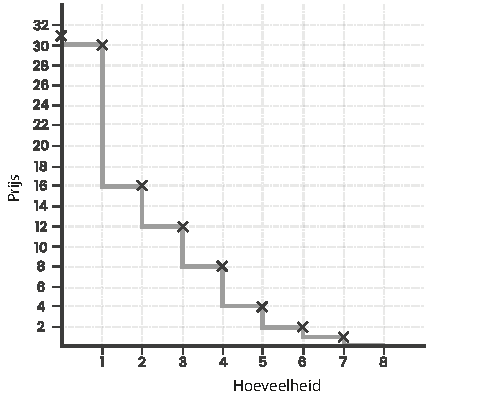
\includegraphics[width=0.7\textwidth]{figures/fig21.pdf}
    \caption[Vraagcurve]{Vraagcurve}
    \label{fig21}
\end{figure}

Zoals uitgelegd in Hoofdstuk 2 waarderen individuen de eerste eenheid van een goed meer dan alle volgende eenheden, en de waardering neemt af naarmate ze meer eenheden aanschaffen. Aan de andere kant zorgt het uitgeven van geld aan eenheden ervoor dat het kassaldo van de koper daalt, waardoor het marginale nut van geld stijgt. Met elke extra eenheid van het goed daalt de marginale prijs\index{prijs} die de koper zou betalen. Dit wijst op \textbf{de wet van de vraag}: \textbf{als de prijs\index{prijs} stijgt, daalt de gevraagde hoeveelheid. Vraagcurves hellen altijd naar beneden, of zijn verticaal, maar ze kunnen niet naar boven buigen, omdat de gevraagde hoeveelheid van een goed niet kan toenemen als de prijs\index{prijs} stijgt.}

Deze analyse is uitgevoerd voor één individu, maar kan worden toegepast op alle individuen in een markt voor een bepaald goed. Door de gevraagde hoeveelheden voor elke persoon bij elk prijspunt op te tellen, krijgen we een curve die de totale marktvraag\index{marktvraag} op een bepaald punt weergeeft. Laten we voor het gemak aannemen dat deze markt bestaat uit 100 consumenten waarvan het gemiddelde wordt vertegenwoordigd door de consument die hierboven is besproken, zodat de gevraagde hoeveelheid 100 keer zo groot is als de waarden in het individuele vraagschema. Omdat de aantallen toenemen en individuele voorkeuren lichtelijk variëren, krijgen we ook een korrelverdeling van hoeveelheden, in plaats van de stapsgewijze functie van de individuele vraagcurve die hierboven is weergegeven.

\begin{table}[H]
\centering
\begin{tabular}{|c|c|}  % Add vertical lines
\hline  % Top horizontal line
    \cellcolor{gray!25}Marktprijs (USD) &
    \cellcolor{gray!25}Gevraagde hoeveelheid rundvlees (pond) \\
\hline  % Horizontal line after the header
 %
 \$31 & 0 \\ \hline
 \$30 & 100 \\ \hline
 \$20 & 170 \\ \hline
 \$16 & 200 \\ \hline
 \$12 & 300 \\ \hline
 \$8 & 400 \\ \hline
 \$4 & 500 \\ \hline
 \$2 & 600 \\ \hline
 \$1 & 700 \\ \hline
 \$0 & 800 \\ \hline  % Bottom horizontal line
\end{tabular}
\caption{Schema van de marktvraag\index{marktvraag}}
\label{tab4}
\end{table}

\begin{figure}[H]
\centering
    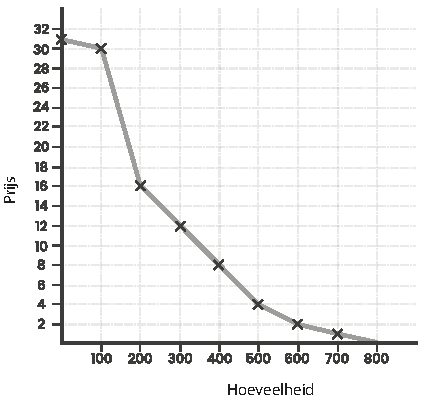
\includegraphics[width=0.7\textwidth]{figures/fig22.pdf}
    \caption[Curve van de marktvraag]{Curve van de marktvraag}
    \label{fig22}
\end{figure}

Aan de aanbodszijde voeren producenten een soortgelijke berekening uit met de goederen die ze verkopen. De persoonlijke voorkeuren van producenten kunnen worden uitgedrukt als een waardeschaal die resulteert in een rangorde van hoeveelheden van het goed ten opzichte van verschillende hoeveelheden geld. In een markteconomie waarin producenten produceren om te verkopen en niet voor hun eigen consumptie\index{consumptie}, zijn de productiekosten de hoofdfactor van de ordinale waardeschaal. Hoe hoger de marktprijs, hoe hoger de verwachte opbrengst van de verkoop en hoe meer middelen kunnen worden besteed aan de productie\index{productie} van meer eenheden van het eindproduct.

Neem als voorbeeld een slager die rundvlees verkoopt aan de voorgenoemde consumenten. Bij een prijs\index{prijs} van \$0 of \$1 per pond zal de slager geen rundvlees verkopen, omdat de prijs\index{prijs} de kosten voor het leveren van het rundvlees niet dekt. Alleen bij een prijs\index{prijs} van \$2 per pond is de slager in staat om te beginnen met produceren en kan hij 10 pond rundvlees leveren. Dit betreft een kleine hoeveelheid die hij kan leveren met een basisinstallatie die hij zich kan veroorloven om tegen die lage prijs\index{prijs} te werken door rundvlees te kopen van de dichtstbijzijnde boerderijen. Bij een prijs\index{prijs} van \$3 per pond kan hij een arbeider inhuren en 30 pond rundvlees leveren. Als hij een prijs\index{prijs} van \$4 per pond rundvlees kan verwachten, kan hij nog een arbeider inhuren en 50 pond leveren. Bij een prijs\index{prijs} van \$5 kan hij 60 pond rundvlees leveren en bij \$6 kan hij 70 pond rundvlees leveren, wat zijn maximale productie is. Verdere prijsstijgingen kunnen zijn capaciteit niet verder verhogen.

\begin{figure}[H]
\centering
    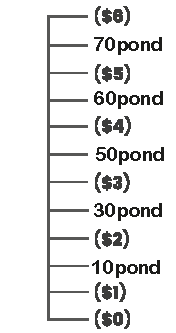
\includegraphics[height=7cm]{figures/fig23.pdf}
    \caption[Ordinale waardeschaal van de producent]{Ordinale waardeschaal van de producent}
    \label{fig23}
\end{figure}

Deze waardeschaal kan ook worden omgezet in een aanbodschema en -curve, die de hoeveelheid tonen die de producent bij elk prijsniveau levert.

\begin{table}[H]
\centering
\begin{tabular}{|c|c|}  % Add vertical lines
\hline  % Top horizontal line
    \cellcolor{gray!25}Marktprijs (USD) &
    \cellcolor{gray!25}Aangeboden hoeveelheid (in pond) \\
\hline  % Horizontal line after the header
 %
 \$7 & 70 \\ \hline
 \$6 & 70 \\ \hline
 \$5 & 60 \\ \hline
 \$4 & 50 \\ \hline
 \$3 & 30 \\ \hline
 \$2 & 10 \\ \hline
 \$1 & 0  \\ \hline
 \$0 & 0  \\ \hline  % Bottom horizontal line
\end{tabular}
\caption{Aanbodschema van de producent}
\label{tab5}
\end{table}

\begin{figure}[H]
\centering
    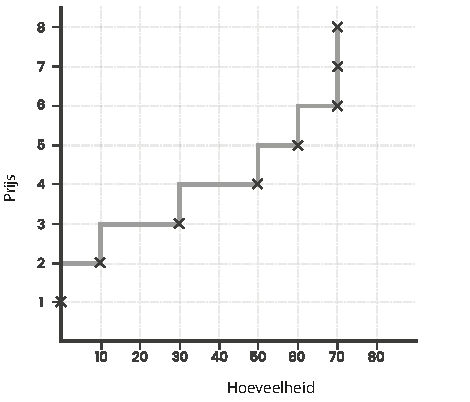
\includegraphics[width=0.7\textwidth]{figures/fig24.pdf}
    \caption[Aanbodcurve van de producent]{Aanbodcurve van de producent}
    \label{fig24}
\end{figure}

\textbf{De wet van het aanbod stelt dat naarmate de prijs\index{prijs} stijgt, de eigenaars van een economisch\index{economisch} goed meer bereid en in staat zijn om grotere hoeveelheden te verkopen. Als gevolg hiervan hellen aanbodcurves alleen omhoog.} Dit kun je begrijpen door te kijken naar de voorkeur van individuen om goederen te bezitten, welke afneemt naarmate de prijs\index{prijs} die ze voor hun goederen kunnen krijgen toeneemt. Voor producenten op de markt kan men ook inzien dat hogere prijzen de stimulans vergroten om meer te gaan produceren en grotere investeringen mogelijk maken om meer grondstoffen en arbeiders te verwerven, wat resulteert in grotere geleverde hoeveelheden.

Voor een goed met meerdere producenten kunnen de aanbodschema\textquotesingle s en -curves van alle producenten worden samengevoegd tot één marktaanbodcurve. De marktaanbodcurve toont de hoeveelheid die door alle producenten van het goed zal worden geproduceerd bij elk gegeven prijsniveau. Laten we voor dit voorbeeld aannemen dat er tien producenten zijn en dat het bovenstaande voorbeeld hun gemiddelde weergeeft.

\begin{table}[H]
\centering
\begin{tabular}{|c|c|}  % Add vertical lines
\hline  % Top horizontal line
    \cellcolor{gray!25}Marktprijs (USD) &
    \cellcolor{gray!25}Aangeboden hoeveelheid (pond) \\
\hline  % Horizontal line after the header
 %
 \$7 & 700 \\ \hline
 \$6 & 700 \\ \hline
 \$5 & 600 \\ \hline
 \$4 & 500 \\ \hline
 \$3 & 300 \\ \hline
 \$2 & 100 \\ \hline
 \$1 & 0  \\ \hline
 \$0 & 0  \\ \hline  % Bottom horizontal line
\end{tabular}
\caption{Aanbodschema van de markt}
\label{tab6}
\end{table}

\begin{figure}[H]
\centering
    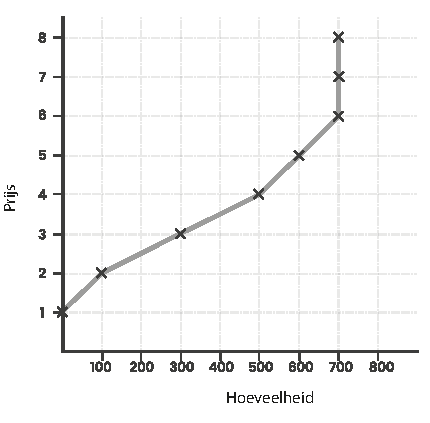
\includegraphics[width=0.7\textwidth]{figures/fig25.pdf}
    \caption[Aanbodcurve van de markt]{Aanbodcurve van de markt}
    \label{fig25}
\end{figure}

\clearpage
\hypertarget{evenwicht}{%
\section{Evenwicht}\label{evenwicht}}

Bij een prijs\index{prijs} van nul is de gevraagde hoeveelheid zeer groot, terwijl de geleverde hoeveelheid waarschijnlijk nul is. Als de prijs\index{prijs} vanaf nul stijgt, neemt de gevraagde hoeveelheid af, terwijl de geleverde hoeveelheid toeneemt. Er is maximaal één prijspunt waarbij de gevraagde en geleverde hoeveelheden gelijk zijn, en dat wordt de \textbf{evenwichtsprijs} genoemd. Dit prijspunt werkt als een magneet op kopers en verkopers en trekt hen aan om hier altijd rond te handelen.

Als de prijs\index{prijs} hoger is dan de evenwichtsprijs, leveren de verkopers een grotere hoeveelheid van het goed dan de kopers vragen, wat resulteert in een \textbf{overschot}. Verkopers zouden de prijs\index{prijs} natuurlijk willen verlagen om meer kopers aan te moedigen hun overtollige goederen te kopen, waardoor de prijs\index{prijs} naar de evenwichtsprijs daalt. Als de prijzen daarentegen lager zijn dan de evenwichtsprijs, dan vragen de consumenten een grotere hoeveelheid dan de verkopers leveren, wat leidt tot een \textbf{tekort.} Dit zou verkopers vervolgens stimuleren om hun prijzen te verhogen om het aanbod te rantsoeneren en hun winst te maximaliseren. Ze kunnen hun prijzen blijven verhogen tot de evenwichtsprijs is bereikt, waarna verdere prijsverhogingen zouden leiden tot minder kopers en een overschot. De dynamiek van de markt zal de prijs\index{prijs} altijd naar de evenwichtsprijs leiden.

We zien het marktevenwicht uit het vorige voorbeeld door de vraag- en aanbodcurves op één grafiek te leggen. Omdat de vraagcurve naar beneden helt, terwijl de aanbodcurve alleen maar stijgt, kunnen de twee curves elkaar slechts op één punt snijden, als ze elkaar al doorkruisen. In deze markt zouden de tien producenten van rundvlees 500 pond rundvlees produceren om te verkopen tegen een prijs\index{prijs} van \$4, en de 100 consumenten zouden dit allemaal kopen tegen een prijs\index{prijs} van \$4. Er zijn geen overschotten of tekorten. Als er veranderingen optreden in de waardeschalen van de individuen, zullen de vraag- en aanbodcurves zich aanpassen om deze veranderingen te weerspiegelen en zal het evenwicht verschuiven, maar het zal kopers en verkopers blijven aantrekken.

\begin{figure}
\centering
    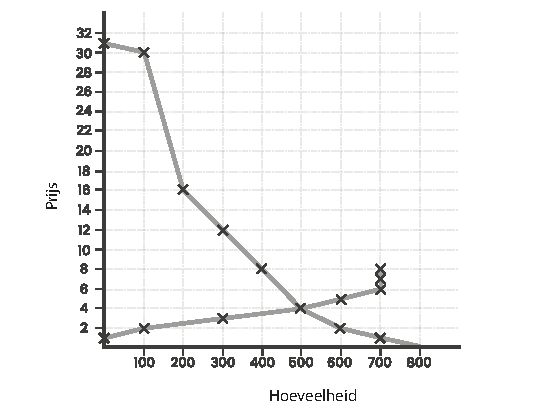
\includegraphics[width=0.8\textwidth]{figures/fig26.pdf}
    \caption[Marktevenwicht]{Marktevenwicht}
    \label{fig26}
\end{figure}

Alle deelnemers aan de markt handelen op manieren die in hun eigen voordeel zijn. Ze stemmen ermee in om aan deze transacties deel te nemen, omdat ze verwachten er voordeel uit te halen, en ze kiezen aan welke transacties ze deelnemen, omdat ze denken dat ze de best mogelijke deal krijgen. Het concept van evenwicht helpt om te begrijpen hoe vrijwillige marktinteracties tot prijzen komen zonder dwingende autoriteit of opgelegd besluit. Toch is het beter om markten\index{markten} te zien als evenwichtsprocessen dan je in te beelden dat markten\index{markten} tot starre evenwichtsprijzen voor alle goederen leiden. De wereld van menselijk handelen\index{menselijk handelen} verandert voortdurend en de voorwaarden van vraag en aanbod worden voortdurend beïnvloed door diverse factoren. Naarmate hun eigen individuele omstandigheden veranderen, verandert ook de realiteit van de markt. Evenwicht is dus geen eindtoestand die markten\index{markten} bereiken. In plaats daarvan zijn markten\index{markten} voortdurende ontdekkingsprocessen waarbij vraag en aanbod zich altijd uitbalanceren naar prijzen die de meeste waarde voor de betrokken deelnemers opleveren.

Prijsschommelingen veranderen de omvang van wat een individu vraagt, grafisch uitgedrukt in de vraagcurves. Maar veranderingen in andere factoren die betrekking hebben op de vraag leiden tot een herformulering van de relatie tussen prijs\index{prijs} en vraag, met een nieuwe gevraagde hoeveelheid voor elke prijs\index{prijs}, en dus een verschuiving in de hele vraagcurve. Enkele factoren die de vraagcurve kunnen verschuiven zijn veranderende voorkeuren, veranderingen in inkomen en welvaart, of veranderende prijzen van andere goederen en diensten. Als het inkomen of de welvaart van de koper toeneemt, zal hij waarschijnlijk meer van de meeste goederen vragen en zal de vraagcurve naar rechts verschuiven, waardoor de gevraagde hoeveelheid bij alle prijsniveaus toeneemt. Maar voor minderwaardige goederen zou een stijging van het inkomen of de rijkdom het tegenovergestelde effect veroorzaken, waarbij de gevraagde hoeveelheid bij alle prijsniveaus afneemt en de vraagcurve naar links verschuift, omdat mensen zich betere alternatieven kunnen veroorloven. Bonen zijn een voorbeeld van zo\textquotesingle n minderwaardig goed: als de inkomens over de hele wereld stijgen, zullen mensen waarschijnlijk hun vraag naar bonen verlagen en hun vraag naar rundvlees verhogen.

De vraagcurve van een goed kan ook worden beïnvloed door veranderingen in de prijzen van andere goederen. Als de prijs\index{prijs} van een goed stijgt, daalt de gevraagde hoeveelheid en daalt de gevraagde hoeveelheid van een aanvullend goed op alle prijsniveaus, waardoor de vraagcurve naar links verschuift. Als datzelfde goed in prijs\index{prijs} daalt, zal de gevraagde hoeveelheid stijgen, terwijl de gevraagde hoeveelheid van het aanvullende goed op alle prijsniveaus zal stijgen, waardoor de vraagcurve naar rechts verschuift. Het tegenovergestelde geldt als het een vervangend goed is.

Behalve door wordt het marktaanbod ook beïnvloed door de productiekosten en de prijzen van verwante producten die met dezelfde productiefactoren kunnen worden geproduceerd. Als de productiekosten van producenten stijgen, kunnen ze lagere hoeveelheden van hun product leveren bij elk prijsniveau, waardoor de aanbodcurve naar links verschuift. Als de producent zich anderzijds realiseert dat hij meer winst kan maken door zijn productiefactoren te verschuiven naar de productie\index{productie} van een ander goed waarvan de prijs\index{prijs} stijgt, zou dat de aanbodcurve voor het oorspronkelijke goed naar links verschuiven, waardoor de geleverde hoeveelheid op alle prijsniveaus daalt.

Dit grafische raamwerk helpt te verklaren hoe een vrije markt reageert op veranderingen in vraag en aanbod in de loop van de tijd. In industrieën waar producenten door technologische innovatie steeds grotere hoeveelheden van een goed tegen een bepaalde prijs\index{prijs} kunnen produceren, resulteert dit in een verschuiving van de aanbodcurve van de markt naar rechts. Het gevolg van deze verschuiving is dat de evenwichtsprijs daalt en de verkochte hoeveelheid toeneemt. Deze trend is te zien in de hightech industrie, waar prijzen voortdurend dalen en de geproduceerde hoeveelheid toeneemt door de verhoogde productiviteit en technologische innovatie. Grafisch kan dit worden geïllustreerd met de verschuiving van S1 naar S2 in Figuur 27.

\begin{figure}[h]
\centering
    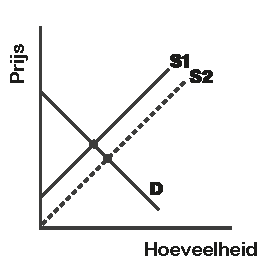
\includegraphics[]{figures/fig27.pdf}
    \caption[Verschuivingen in de aanbodcurve]{Verschuivingen in de aanbodcurve}
    \label{fig27}
\end{figure}

Als het omgekeerde zou gebeuren, en een probleem met de aanbodketen de productie\index{productie} van het goed negatief zou beïnvloeden, zouden producenten een kleinere hoeveelheid van het goed kunnen leveren bij elk gegeven prijsniveau, waardoor de aanbodcurve effectief naar links zou verschuiven. In deze situatie zou het nieuwe evenwicht met de vraagcurve ontstaan bij een hogere prijs\index{prijs} en een lagere hoeveelheid. Een natuurramp is hier een extreem voorbeeld van, waarbij de beschikbare hoeveelheden van een goed enorm afnemen, terwijl de prijzen stijgen. Dit wordt grafisch weergegeven met de verschuiving van S2 naar S1 in Figuur 27.

We kunnen dezelfde analyse toepassen op verschuivingen in de vraagcurve. Factoren die de vraag van de consument bij alle prijzen doen toenemen, zoals een toegenomen voorkeur van de consument voor het goed ongeacht de prijs\index{prijs}, of een stijging van de prijs\index{prijs} van vervangende goederen of een daling van de prijs\index{prijs} van aanvullende goederen, zouden de vraagcurve naar rechts doen verschuiven, grafisch weergegeven als de verschuiving van curve D1 naar curve D2 in Figuur 28. Een daling van de consumentenvraag naar het goed tegen alle prijzen, of een stijging van de prijs\index{prijs} van aanvullende goederen of een daling van de prijs\index{prijs} van een vervangend goed, zou de vraagcurve naar links doen verschuiven. Grafisch wordt dit weergegeven door de verschuiving van curve D2 naar D1 in Figuur 28.

\begin{figure}[h]
\centering
    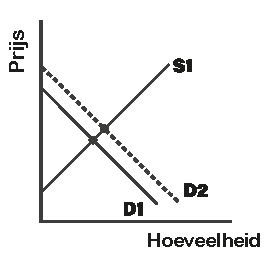
\includegraphics[]{figures/fig28.pdf}
    \caption[Verschuivingen in de vraagcurve]{Verschuivingen in de vraagcurve}
    \label{fig28}
\end{figure}

\hypertarget{markten-van-producentgoederen}{%
\section{Markten van producentgoederen}\label{markten-van-producentgoederen}}

Producenten baseren hun beslissingen ook op het nut dat verschillende handelsmethoden hun opleveren. Het verschil tussen de keuze van de consument en die van de producent ligt aan het feit dat de producent geen persoonlijk nut ontleent aan de factoren die hij gebruikt; hij gebruikt ze puur om de geldelijke winst die hij met zijn bedrijf\index{bedrijf} kan behalen te maximaliseren. Consumentensoevereiniteit betekent dat de producent al zijn zakelijke beslissingen baseert op de wensen en behoeften van de consument.

Het productieproces\index{productieproces} bestaat uit het omzetten van productiefactoren in eindgoederen en -diensten die aan consumenten worden verkocht. De hoeveelheid van elke ingezette productiefactor wordt bepaald door de kosten ervan te vergelijken met de marginale inkomsten die ze bijdraagt aan de bedrijfsactiviteiten. Elke extra eenheid arbeid of kapitaal\index{kapitaal} die in de productie\index{productie} wordt ingezet, resulteert in een marginale toename van de hoeveelheid geproduceerde eindproducten. Werkgevers zullen productiefactoren blijven inzetten zolang de verwachte marginale opbrengst van de ingezette factor hoger is dan de kosten van het inzetten ervan. De prijzen van deze productiefactoren worden op hun beurt bepaald door hoe goed ze voldoen aan de vraag van de consument. Als het inhuren van een extra arbeider voor een dag naar verwachting \$10 aan inkomsten zal toevoegen aan een bedrijf\index{bedrijf}, zal dat bedrijf\index{bedrijf} alleen een extra arbeider inhuren als de vraag naar loon minder is dan \$10 per dag. Als een ondernemer overweegt om een machine te kopen die \$1.000 kost, zal hij deze alleen kopen als de verwachte marginale verdiscontering van het product dat het gedurende zijn levensduur produceert groter is dan \$1.000. Uiteindelijk is het dus de waardering van eindproducten door de consument die waarde geeft aan productiefactoren. De functie van de ondernemer is om uitspraken te doen over de toekomstige behoeften van consumenten, te investeren in de productiefactoren voordat de productie\index{productie} plaatsvindt, en het risico\index{risico} op zich te nemen dat hij het mis heeft over wat consumenten zullen waarderen na de productie\index{productie}.

Het is zinloos om te klagen over lonen of kapitaalopbrengsten. Dit zijn cruciale signalen van de markt die individuen vertellen hoe waardevol hun arbeid, land en kapitaal\index{kapitaal} zijn. Ondernemers kunnen niet zomaar zelf de lonen bepalen; ze zijn afhankelijk van de subjectieve waarderingen van consumenten. Als een ondernemer besluit om te veel te betalen voor lonen, zal hij zijn winstgevendheid verliezen en vervangen worden door ondernemers die een gepastere prijs\index{prijs} betalen. Als de ondernemer besluit een lager loon te betalen, zal hij zijn werknemers verliezen aan anderen die bereid zijn een hogere prijs\index{prijs} te betalen. Om ondernemer te blijven in een bepaalde branche, heeft de ondernemer geen andere keuze dan werknemers te betalen voor hun marginale productiviteit. In een vrijemarktsysteem kunnen kapitalisten en ondernemers de werknemers niet onderdrukken, omdat ze vrij zijn om elders te gaan werken en omdat de consumenten hun producten elders kunnen kopen. Alleen door zorgvuldig en correct te koorddansen tussen werknemers en consumenten kunnen ondernemers in bedrijf\index{bedrijf} blijven.

\hypertarget{economisch-handelen-in-de-marktorde}{%
\section{Economisch handelen in de marktorde}\label{economisch-handelen-in-de-marktorde}}

We kunnen het marktsysteem zien als het grotere kader waarbinnen al het eerder besproken economisch\index{economisch} handelen kan plaatsvinden met de grootste toename in productiviteit. Arbeid, kapitaal\index{kapitaal}, technologie, macht, handel en geld zijn allemaal instrumenten die veel productiever kunnen worden ingezet in de context van vrije en onpersoonlijke ruilhandel\index{ruilhandel} op de markt. Als gevolg hiervan heeft de markteconomie de reële lonen van arbeiders gestaag verhoogd, omdat de markteconomie voortdurend nieuwe manieren vindt om de waarde van menselijke tijd te verhogen, door deze op de meest productieve manier te gebruiken om aan de behoeften van andere mensen te voldoen.

Marktdeelnemers communiceren hun veranderende voorkeuren en voorwaarden aan elkaar door te beslissen om tegen bepaalde prijzen wel of niet te kopen. Dit proces van wederzijdse samenwerking stelt alle marktdeelnemers in staat om in hun eigen belang te handelen, terwijl ze hun handelingen coördineren om elkaar beter van dienst te zijn. Alle voorkeuren van consumenten worden aan andere marktdeelnemers kenbaar gemaakt door hun keuzes om tegen een bepaalde prijs\index{prijs} wel of niet te kopen, waardoor producenten waardevolle kennis krijgen waarmee ze hun productiebeslissingen kunnen maken. Zoals Mises het stelde:

\begin{blockquotebox}
    Het marktproces is de aanpassing van de individuele handelingen van de verschillende marktdeelnemers aan de vereisten van onderlinge samenwerking. De marktprijzen vertellen de producenten wat ze moeten produceren, hoe ze moeten produceren en in welke hoeveelheid. De markt is het brandpunt waar de activiteiten van de individuen samenkomen.\footnotemark    
\end{blockquotebox}
\footautocite{125}

Mises voegt hier verder aan toe:

\begin{blockquotebox}
    In de natuur heersen onverzoenlijke belangenconflicten. De middelen voor levensonderhoud zijn schaars. De groei van populaties heeft de neiging om het bestaansminimum te overtreffen. Alleen de sterkste planten en dieren overleven. De vijandschap tussen een dier dat verhongert en een ander dat het voedsel wegkaapt is onverbiddelijk. Sociale samenwerking door arbeidsdeling\index{arbeidsdeling} lost zulke vijandigheid op. Het vervangt vijandigheid door samenwerking en wederkerigheid. De leden van de samenleving zijn verenigd in een gemeenschappelijke onderneming.\footnotemark    
\end{blockquotebox}
\footautocite{126}

\hypertarget{consumentensoevereiniteit}{%
\section{Consumentensoevereiniteit}\label{consumentensoevereiniteit}}

De zorgvuldige analyse van het marktproces illustreert waarom de consument in een vrije markt koning is. Individuen zijn in een markteconomie soeverein in hun hoedanigheid als consument, omdat de producenten geen manier hebben om hen te dwingen hun goederen te kopen, behalve door goederen te produceren die voldoen aan de behoeften en verlangens van de consument tegen een prijs\index{prijs} die zij zich kunnen veroorloven. Producenten investeren hun kapitaal\index{kapitaal} in het productieproces\index{productieproces} en zijn afhankelijk consumenten die hun product goed vinden, zodat hun investering niet verloren gaat. Producenten bevinden zich niet in een positie om de voorwaarden te dicteren of consumenten uit te buiten; die hebben alle keuze. Zoals Mises uitlegt:

\begin{blockquotebox}
    Als ze er niet op uit waren om op de goedkoopste markt aankopen te doen en hun productiefactoren zo in te richten dat ze op de beste en goedkoopste manier aan de vraag van de consumenten konden voldoen, dan zouden ze gedwongen worden om hun bedrijf\index{bedrijf} te stoppen. Efficiëntere mensen die er beter in slagen de productiefactoren te kopen en te verwerken, zouden hen vervangen. De consument bevindt zich in een positie waarin hij zijn opwellingen en wensen de vrije loop kan laten. De ondernemers, kapitalisten en boeren hebben geen keuze; ze zijn verplicht om zich in hun bedrijfsvoering te houden aan de wensen van het kopende publiek. Elke afwijking van de lijnen die zijn voorgeschreven door de vraag van de consumenten is voor eigen rekening. De kleinste afwijking, bewust gekozen of veroorzaakt door fouten, slecht beoordelingsvermogen of onnauwkeurigheid, beperkt hun winsten of doet ze zelfs helemaal verdwijnen. Een ernstigere afwijking resulteert in verliezen en tast zo hun vermogen aan of slokt dit volledig op. Kapitalisten, ondernemers en landeigenaren kunnen hun rijkdom alleen behouden en vergroten door de orders van consumenten zo goed mogelijk uit te voeren.\footnotemark    
\end{blockquotebox}
\footautocite{127}

Mises vergelijkt de macht van consumenten in de markt vervolgens met het democratische proces en laat zien dat het superieur is, omdat het tegemoet komt aan de behoeften van iedereen, terwijl democratie alleen tegemoet komt aan de behoeften van de winnende meerderheid:

\begin{blockquotebox}
    Met elke cent die wordt uitgegeven bepalen de consumenten de richting van alle productieprocessen en de details van de organisatie van alle bedrijfsactiviteiten. Deze stand van zaken is beschreven door de markt een democratie te noemen waarin elke cent het recht geeft om te stemmen. Het zou correcter zijn om te zeggen dat een democratische grondwet een plan is om aan de burgers in het bestuur dezelfde macht toe te kennen die de markteconomie hen geeft in hun mogelijkheden als consumenten. De vergelijking is echter niet perfect. In de politieke democratie zijn alleen de stemmen die uitgebracht worden voor de kandidaat of het plan van de meerderheid effectief om de gang van zaken vorm te geven. De stemmen van de minderheid hebben geen directe invloed op het beleid. Maar op de markt wordt geen enkele stem tevergeefs uitgebracht. Elke cent die wordt uitgegeven heeft de macht om de productieprocessen te beïnvloeden. Boekuitgevers bedienen niet alleen de meerderheid door detectives te publiceren, maar ook de minderheid die lyrische poëzie en filosofische geschriften leest. De bakkerijen bakken niet alleen brood voor gezonde mensen, maar ook voor zieken met een speciaal dieet. De beslissing van een consument wordt uitgevoerd met de volledige vaart die hij er achter zet met zijn bereidheid om een bepaald geldbedrag uit te geven.\footnotemark    
\end{blockquotebox}
\footautocite{128}

\hypertarget{een-contrast-van-benaderingen}{%
\section{Een contrast van benaderingen}\label{een-contrast-van-benaderingen}}

Al zolang er regeringen bestaan, bestaat de drang om prijzen per wet vast te stellen. Dit heeft geleid tot een hele reeks verschrikkelijke en voorspelbare gevolgen.\autocite{129} Maar de vele en diverse vergeefse pogingen van centrale overheden om prijzen vast te leggen hebben één positief gevolg gehad: ze hebben veel mensen laten inzien dat economie een product is van menselijk handelen\index{menselijk handelen}, ook al verwoorden ze het misschien niet helemaal in deze Misesiaanse bewoordingen. Door de analyse van de politicus die de prijscontrole oplegt en die van de econoom tegenover elkaar te zetten, zien we duidelijk de kracht van de economische manier van denken.

De politicus die ontevreden is over een marktprijs en deze wil veranderen, ziet de prijs\index{prijs} als iets willekeurigs dat hij kan bepalen. Hij denkt niet op een economische manier omdat hij prijzen niet ziet als het resultaat van menselijk handelen\index{menselijk handelen}, als een weerspiegeling van menselijke keuzes. Het element van individuele en persoonlijke keuze bij het bepalen van prijzen wordt genegeerd. De aandacht gaat in plaats daarvan naar de politieke en sociale implicaties van deze prijzen. Hij vergelijkt de huidige realiteit met een hypothetische realiteit waarin de prijs\index{prijs} lager is en de geconsumeerde hoeveelheid hoger, terwijl al het andere hetzelfde blijft.

De meeste politieke leiders zijn niet op hun positie gekomen door hun economische kennis. Het begrijpen van economie is wellicht een belangrijke belemmering voor succes in de politiek. Politici beschouwen de prijzen van economische goederen en diensten louter als een maatstaf voor hun betaalbaarheid en ze weten dat hoe lager de prijzen, hoe gelukkiger de bevolking. Zonder prijzen te begrijpen als het resultaat van menselijk handelen\index{menselijk handelen} in reactie op de economische realiteit, denkt de politicus dat hij prijzen kan sturen om zijn gewenste resultaten te bereiken en dus zal hij wetten aannemen die maximumprijzen voor specifieke goederen voorschrijven. De foutieve redenering gaat ervan uit dat als de prijs\index{prijs} van een goed wettelijk wordt vastgelegd, kopers en verkopers geen andere keuze hebben dan tegen die prijs\index{prijs} te kopen en te verkopen.

Als de politieke leider een econoom wil raadplegen, zal hij waarschijnlijk de voorkeur geven aan het advies van kwantitatieve economen die schijnbaar correcte argumenten voor dit beleid kunnen produceren. Een kwantitatief econoom kan het effect van prijzen op economische activiteit wiskundig modelleren en een theoretisch kwantitatief verband vinden tussen de prijs\index{prijs} van een goed, het bestedingsniveau in de economie en economische groei. Het is mogelijk om een causaal mechanisme te veronderstellen, gebaseerd op gegevens uit de echte wereld, waarbij een verlaging van de prijs\index{prijs} van een essentieel goed de levensstandaard van een groot deel van de bevolking verhoogt, wat resulteert in meer sparen, meer investeringen en een snellere economische groei. Met een kwantitatieve observatie van de grootheden en ontoetsbare aannames over de richting van causaliteit kan de kwantitatieve econoom de overheid\index{overheid} een schijnbaar wetenschappelijke formule aanreiken om de economie te verbeteren door prijzen bij wet op te leggen. Zonder een constante meeteenheid kunnen deze vergelijkingen niet nauwkeurig zijn, zodat elk gewenst resultaat kan worden geregeld.

Vanuit het perspectief van de degelijke econoom is de prijs\index{prijs} echter meer dan alleen een maatstaf voor de betaalbaarheid van een goed. Het is een product van vrijwillige menselijke handelingen en keuze en de oplossing van een calculatieprobleem voor de producent en consument. Als de overheid\index{overheid} een andere prijs\index{prijs} voor het goed oplegt, is er geen garantie dat de betrokken individuen dezelfde handelingen zullen verrichten die ze anders ook hadden verricht, noch dat ze elkaar op dezelfde manier tevreden kunnen stellen.

Prijzen zijn geen willekeurige getallen die door winkeliers worden bedacht, ze komen tot stand door een complex samenspel van mensen die handelen en vraag en aanbod op de markt beïnvloeden. Een markttransactie die plaatsvindt tegen een bepaalde prijs\index{prijs} geeft aan dat zowel de koper als de verkoper ervoor gekozen hebben om deze prijs\index{prijs} te accepteren. Beiden hadden natuurlijk liever een andere prijs\index{prijs} gezien; de koper had liever een lagere prijs\index{prijs} gezien en de verkoper had liever een hogere prijs\index{prijs} gezien, maar de huidige prijs\index{prijs} was duidelijk aanvaardbaar voor beiden, gezien het feit dat ze handel dreven. Als een politicus tussenbeide zou komen en de prijs\index{prijs} bij wet met dwang te veranderen, is er geen reden om aan te nemen dat de koper en verkoper dezelfde beslissingen zouden nemen als voorheen. En vanuit het perspectief van een econoom zou zo\textquotesingle n wet veel destructiever zijn dan de prijzen die op de markt waren ontstaan, hoe onaangenaam die ook waren voor de leiders.

Wat de marktprijs van een goed ons vertelt, is dat de verkoper tevreden is met de verkoop van dit goed voor deze prijs\index{prijs}. Als kopers weigeren dit goed voor die prijs\index{prijs} te kopen, dan moet de producent zijn prijzen verlagen. Als hij zijn prijs\index{prijs} niet kan verlagen om aan de waardebepaling van de consument te voldoen, dan wordt het goed niet geproduceerd. Om een bedrijf\index{bedrijf} een bepaald goed te laten verkopen, moet de prijs\index{prijs} de producent compenseren voor alle kosten en de opportuniteitskosten die hij maakt om het product beschikbaar te maken. Wanneer prijscontrole een maximumprijs voor een goed vastlegt die onder de kosten van de producent ligt, dan zal de producent gewoon stoppen met de verkoop ervan, wat leidt tot tekorten.

Producenten, die hun eigen belangen dienen, zullen een goed niet verkopen voor een prijs\index{prijs} die niet hun volledige productiekosten dekt. Ze staken hun bedrijf\index{bedrijf} liever om thuis te zitten, dan dat ze in een bedrijf\index{bedrijf} werken dat hen geld kost. Dus proberen om lagere prijzen af te dwingen resulteert simpelweg in het wegnemen van de menselijke stimulans om een goed te produceren, wat resulteert in hogere prijzen en nog lager aanbod. Het andere onvermijdelijke gevolg van prijscontroles is het ontstaan van zwarte markten\index{markten} waar verkoper en koper kunnen handelen met prijzen die voor beiden passend zijn, buiten de aandacht van de overheid\index{overheid} om.

\hypertarget{kapitalisme}{%
\chapter{Kapitalisme}\label{kapitalisme}}

\vspace{1em}
\begin{blockquotebox}
    Uit de geschiedenis blijkt duidelijk dat privaat eigendom fundamenteel is, en onlosmakelijk verbonden is met een beschaving\index{beschaving}.\footnotemark
    \par\raggedleft--- Ludwig von Mises\index{Ludwig von Mises}    
\end{blockquotebox}
\autocite{130}

\vspace{2em}

Een markteconomie, zoals besproken in het vorige hoofdstuk, betreft een sociale orde waarbij personen vanuit hun eigen belang economisch\index{economisch} handelen, hetgeen ten goede komt aan alle betrokken partijen. Alle vormen van economisch handelen door individuen, zoals arbeid, kapitaalopbouw, technologische vernieuwing, handel en de productie van moderne energie, worden op vrijwillige basis door individuen uitgevoerd. Deze individuen maken gebruik van geldmiddelen om hun productiebereik\index{productie} uit te breiden en hun materiële welzijn aanzienlijk te verhogen in vergelijking met wat ze elk afzonderlijk zouden kunnen realiseren. De uitgebreide monetaire markteconomie faciliteert het ontstaan van het kapitalisme\index{kapitalisme}, een systeem van privaat eigendom van kapitaalgoederen\index{kapitaalgoederen} waarin individuen vrij zijn om kapitaal\index{kapitaal} aan te kopen en te verkopen en beslissingen te nemen over de inzet van hun kapitaal. Hierbij genieten ze de voordelen van productief gebruik ervan en dragen ze de nadelen van onproductief gebruik.



In \emph{The End of Socialism and the Calculation Debate Revisited} legt Rothbard de criteria van Mises voor een markteconomie uit:

\begin{blockquotebox}
    Tijdens één van Mises\textquotesingle{} seminaries aan de New York University, vroeg ik hem of hij, gezien het brede spectrum van economieën van een zuivere vrije markt tot puur totalitarisme, één criterium kon aanwijzen op basis waarvan hij kon zeggen dat een economie in wezen ``socialistisch'' was of dat het een markteconomie was. Enigszins tot mijn verbazing antwoordde hij onmiddellijk: ``Ja, de sleutel is of de economie een aandelenmarkt heeft.'' Anders gezegd, of de economie een volwaardige markt heeft in eigendomstitels van land en kapitaalgoederen\index{kapitaalgoederen}. Kortom: wordt de toewijzing van kapitaal\index{kapitaal} in principe bepaald door de overheid\index{overheid} of door particuliere eigenaren?\footnotemark
\end{blockquotebox}
\autocite{131}

Voor Mises en de Oostenrijkse economen geldt de aanwezigheid van een aandelenmarkt als een effectieve toetssteen voor het kapitalisme\index{kapitalisme}, omdat het een duidelijk kenmerk is van een vrije markt voor productiemiddelen, toegankelijk voor iedereen in de maatschappij. Dit mechanisme zorgt ervoor dat kapitaal\index{kapitaal} terechtkomt bij degenen die het het meest productief kunnen inzetten. Bedrijven die genoteerd staan op de aandelenmarkt bezitten een significant deel van het productiekapitaal in een samenleving, en dit kapitaal is voor iedereen beschikbaar om naar wens te kopen en verkopen. Als iemand meent dat hij kapitaalgoederen\index{kapitaalgoederen} productiever kan inzetten dan de huidige eigenaar, kan hij deze overkopen door de gangbare marktprijs\index{prijs} voor de aandelen te betalen. Iedereen is in staat om zijn spaargeld te investeren in een productieproces\index{productieproces} dat naar verwachting meer opbrengt dan het simpelweg aanhouden van contant geld. Degenen die succesvol zijn in het productief inzetten van hun kapitaal\index{kapitaal}, maken winst en krijgen toegang tot meer kapitaalgoederen\index{kapitaalgoederen}. Aan de andere kant zullen diegenen die hun kapitaal\index{kapitaal} onproductief gebruiken, verliezen lijden, waardoor hun bezit een onhoudbare en kostbare vergissing wordt. Dit moedigt hen aan hun kapitaal\index{kapitaal} te verkopen aan kopers die bereid zijn een hogere prijs\index{prijs} te betalen omdat zij menen de middelen productiever te kunnen inzetten. Met een aandelenmarkt en een vrij kapitaalmarktmechanisme bestaan er geen beschermingsmechanismen voor kapitaaleigenaren die hun middelen ineffectief inzetten. Ze zullen hun bezit uiteindelijk verkopen aan efficiëntere gebruikers of blijven verliezen maken tot hun kapitaal volledig is uitgeput. In beide gevallen is kapitaal\index{kapitaal} altijd onderdeel van een proces waarbij het verschuift naar meer productieve en bekwame handen. In een vrijemarkteconomie kunnen privileges of mandaten deze onstuitbare verschuiving naar een productiever gebruik van kapitaal\index{kapitaal} principieel niet tegenhouden.

Economen van de Oostenrijkse School\index{Oostenrijkse School} bieden, door kapitalisme\index{kapitalisme} te definiëren en te verklaren binnen de context van menselijk handelen\index{menselijk handelen}, de meest uitgebreide en coherente benadering van kapitalisme\index{kapitalisme}. Hun visie dient als een krachtig en praktisch analytisch instrument voor het begrijpen van economische vraagstukken in de echte wereld en de dynamiek van een kapitalistisch systeem. Dit contrasteert sterk met de oppervlakkige behandeling van het onderwerp door andere economische scholen. Marxistische economen beschouwen kapitaal\index{kapitaal} als een kwaadaardige kracht die kapitaalbezitters in staat stelt anderen uit te buiten en te onderdrukken. Ze negeren vaak de voordelen die kapitaal\index{kapitaal} aan werknemers biedt, zoals verhoogde productiviteit, de kosten verbonden aan het bezitten ervan in de vorm van opportuniteitskosten, en de verantwoordelijkheden en risico's\index{risico} die eigendom met zich meebrengt. Tegelijkertijd beschouwen de meeste mainstream economen kapitaal\index{kapitaal} als een geaggregeerd geheel --- een homogene massa die zelfonderhoudend is en ingezet wordt voor productie\index{productie}. Beide perspectieven missen het belang van privaat eigendom voor de groei van kapitaal\index{kapitaal} en de essentiële rol van een vrije markt in het toewijzen van kapitaal\index{kapitaal} aan de meest productieve toepassingen. Door de cruciale functie van kapitaalmarkten over het hoofd te zien, laten beide economische scholen hun aanhangers verkeerdelijk geloven dat kapitalistische economische productie\index{productie} kan bestaan in een systeem met beperkt privaat eigendom en vrije handel van productiemiddelen.

De waarde van kapitaalgoederen\index{kapitaalgoederen} is subjectief en hangt af van hoe individuen ze waarderen. Ze is niet inherent of intrinsiek aanwezig. Of iets al dan niet een kapitaalgoed\index{kapitaalgoederen} is, hangt volledig af van het oordeel en de handelingen van de persoon die het in bezit heeft. Bijvoorbeeld, een computer ingezet om games te spelen, geldt als een consumptiegoed\index{consumptiegoed}. Dezelfde computer van een professionele grafisch ontwerper wordt echter beschouwd als een kapitaalgoed\index{kapitaalgoederen}. Zonder de mogelijkheid om kapitaalgoederen\index{kapitaalgoederen} te kopen met de bedoeling om winst te maken, hebben mensen weinig motivatie om kapitaal\index{kapitaal} te verzamelen en te behouden. Als er geen kans is om kapitaal\index{kapitaal} te ruilen voor financieel voordeel, ontbreekt het mechanisme om te garanderen dat kapitaal\index{kapitaal} productief wordt ingezet. Hierdoor voorkomt men dat het in handen valt van mensen die het verspillen en de waarde ervan verlagen. Kapitaal moet men niet zien als een verzameling machines, maar als een concept dat, net als een levend organisme, overleeft in een ecosysteem. In dit ecosysteem wordt het voortdurend gewaardeerd en verhandeld door actieve individuen. Daarom is het niet zinvol om te praten over een kapitaalvoorraad in een samenleving zonder rekening te houden met de individuen. Zij waarderen de kapitaalgoederen\index{kapitaalgoederen} zonder beperkingen, zetten ze in voor productie\index{productie} en profiteren ervan. Kapitaal zonder markteconomie is zoals een vis op het droge: een slap, levenloos omhulsel van wat ooit was.

\hypertarget{kapitaalmarkten}{%
\section{Kapitaalmarkten}\label{kapitaalmarkten}}

Het komt vaak voor dat leken, politici en mainstream economen landen bestempelen als zijnde socialistisch of kapitalistisch, zonder daarbij een heldere definitie te hanteren om deze labels te rechtvaardigen. De criteria van Mises bieden ons echter een zeer effectieve methode om te begrijpen wat een kapitalistische economie inhoudt en wat een socialistische economie kenmerkt.

Een economie die geen aandelenmarkt heeft ontwikkeld, is geen kapitalistische markteconomie, omdat het niet het niveau van economische specialisatie en een verlengde kapitaalstructuur van de productie\index{productie} heeft ontwikkeld die nodig zijn om een markt voor kapitaal\index{kapitaal} te ontwikkelen. Een economie waarvan de aandelenmarkt onder dwang door de overheid\index{overheid} wordt gesloten, is een socialistische economie, omdat het kapitaal\index{kapitaal} uit het domein van de marktconcurrentie is weggehaald en in handen is gegeven van bureaucraten die het niet bezitten, er niet legitiem van kunnen profiteren en geen economische calculatie te kunnen verrichten om te beslissen wat de beste productiemethoden zijn om het te gebruiken. Het criterium van Mises stelt ons in staat om economieën in te delen in drie categorieën: pre-kapitalistisch, kapitalistisch en socialistisch. De geschiedenis van de meeste landen in de wereld is de positieve ontwikkeling van pre-kapitalisme\index{kapitalisme} naar kapitalisme\index{kapitalisme}, onderbroken door rampzalige omleidingen naar socialistische verwoesting.

De Russische aandelenmarkt werd in het begin van de achttiende eeuw opgericht door een decreet van Peter de Grote. Dit was een tijd waarin Rusland zich ontwikkelde van een agrarische naar een kapitalistische economie. De beurzen bleven functioneren tot de bolsjewieken in 1917 door een staatsgreep aan de macht kwamen en Rusland overging op een socialistisch economisch\index{economisch} systeem. Na het einde van het bolsjewistische regime hervatte de aandelenmarkt zijn activiteiten in 1991, waarmee het land terugkeerde naar een kapitalistische economie. De verwoestende impact van het socialisme op Rusland valt samen met de periode waarin de aandelenmarkt was gesloten.

Duitsland biedt een ander inzichtelijk voorbeeld van het belang van de criteria van Mises. Al in de zestiende eeuw werden verschillende effectenbeurzen opgezet in Hamburg, Frankfurt en andere Duitse steden. In 1815 begon de beurs van Hamburg met het verhandelen van bedrijfsaandelen, wat een belangrijk moment was in de ontwikkeling van Duitsland naar een moderne kapitalistische economie. De Duitse aandelenmarkten bleven actief tot de Nationaal Socialistische Partij onder leiding van Adolf Hitler in 1933 aan de macht kwam. Vervolgens werden alle bedrijven gedwongen om zich bij kartels aan te sluiten en kwam hun kapitaal\index{kapitaal} onder controle van het naziregime.

De \emph{Deutsche Börse Group} beschrijft deze episode als volgt: ``Met de machtsovername door de nazi\textquotesingle s in 1933 werd het algemene economische beleid opgenomen in het algemene regerings- en oorlogsbeleid. Het toezicht op de beurzen werd weggehaald bij de deelstaten en werd het domein van de centrale overheid\index{overheid}, waarbij het aantal beurzen werd teruggebracht van 21 naar 9. De beurs van Frankfurt nam de beurs van Mannheim in 1935 over. De gefuseerde instelling werd de Rijn-Main Beurs genoemd. Hoewel de beurs van Frankfurt bleef functioneren als een \textquotesingle binnenlandse beurs\textquotesingle, had het in werkelijkheid geen belangrijke functie. De economische controle van de nazi\textquotesingle s beperkte de ontwikkeling van de vrije markt en de aandelenhandel. Over het algemeen werd gedacht dat potentiële kapitaalgoederen\index{kapitaalgoederen} alleen ten goede kwamen aan de oorlogseconomie en niet langer konden worden geïnvesteerd in grotere obligaties of aandelen.''\autocite{132}

Na de val van het naziregime ontwikkelde het westen van Duitsland zich tot een kapitalistische economie, waarbij de aandelenbeurzen weer als een vrije markt gingen functioneren. Het oosten van het land behield daarentegen een socialistische economie en kende geen werkende beurzen tot aan de Duitse hereniging in 1990.

Polen dient eveneens als een leerzaam voorbeeld. De eerste Poolse beurs werd opgericht in 1817 en begon in de jaren 1840 met de handel in bedrijfsaandelen. Deze beurs bleef operationeel tot 1915, toen deze sloot vanwege de ineenstorting van de Poolse economie tijdens de Eerste Wereldoorlog\index{Eerste Wereldoorlog}. In 1919 werd de beurs opnieuw geopend, waarmee Polen terugkeerde naar een kapitalistische economie, tot het land in 1939 gezamenlijk werd binnengevallen door de nazi-sovjetalliantie en de controle werd verdeeld tussen Duitsland en Rusland. Na de nederlaag van de nazi's in 1945, kwam geheel Polen, nog steeds zonder functionerende beurs, onder controle van de Sovjet-Unie. Dit leidde het land naar socialistische armoede en economisch\index{economisch} falen tot 1991, toen het socialistische economische systeem van Polen instortte en een vrijemarkteconomie werd ingevoerd. In april 1991 werd de aandelenmarkt opnieuw geopend.\autocite{133}

In alle drie de genoemde landen fungeert het bestaan van een aandelenmarkt als een betrouwbare indicator voor de economische transitie tussen pre-kapitalistische, kapitalistische en socialistische vormen van economische organisatie. Het is geen toeval dat in deze landen de periodes zonder aandelenmarkt samenvielen met armoede, oorlog\index{oorlog} en omvangrijke vernietiging van kapitaalmiddelen.

Tegenwoordig is het een veelvoorkomend verschijnsel dat politici, vooral in de Verenigde Staten\index{Verenigde Staten} en in ontwikkelingslanden, Scandinavische landen aanhalen als voorbeelden van succesvolle socialistische regimes. Echter, de beurzen in alle Scandinavische landen zijn al meer dan een eeuw onafgebroken operationeel. De Deense beurs is actief sinds 1808, de Zweedse sinds 1863, de Noorse sinds 1881, en de Finse sinds 1912.\autocite{134} Geen van de Scandinavische aandelenmarkten is ooit overgenomen door een regering, wat betekent dat de verdeling van eigendom en kapitaal\index{kapitaal} in al deze economieën altijd is geleid door de voorkeuren en acties van vrij handelende individuen, en niet door dwingende opdrachten van een centrale overheidsinstantie. In tegenstelling tot de vaak onsamenhangende en emotioneel geladen publieke discussies over dit thema, biedt Mises heldere criteria om te bepalen wat een socialistisch economisch\index{economisch} systeem inhoudt.

\hypertarget{kapitalisme-is-ondernemend-niet-bureaucratisch}{%
\section{Kapitalisme is ondernemend, niet bureaucratisch}\label{kapitalisme-is-ondernemend-niet-bureaucratisch}}

Het belang van privaat eigendom van productiemiddelen voor het economische systeem wordt duidelijk in, en geïllustreerd door, Mises' uitleg van het kapitalisme\index{kapitalisme} als een ondernemend systeem, in tegenstelling tot een bureaucratisch systeem. De verwarring rond dit subtiele onderscheid ligt aan de basis van alle pogingen om de markteconomie opzij te zetten ten gunste van centrale planning. In een kapitalistische economie manifesteert de arbeidsdeling\index{arbeidsdeling} zich in het investeringsproces zelf, dat verdeeld is over drie verschillende rollen: de kapitalist, de ondernemer en de manager. Het proces start met de kapitalist, die kiest om consumptie\index{consumptie} uit te stellen en in plaats daarvan te sparen en later te investeren. In een moderne kapitalistische economie kan de investeerder zijn geld op de financiële markten\index{markten} plaatsen, waarbij het verspreid wordt over verschillende productielijnen en bedrijven. De investeerder kan zelf besluiten waar het geld naartoe gaat, of hij kan deze taak overlaten aan een professionele investeerder die het kapitaal\index{kapitaal} over verschillende economische doelen verdeelt. Deze allocatie van kapitaal\index{kapitaal} is de ondernemersfunctie binnen de markten\index{markten}. Nadat het geld is verdeeld over verschillende bedrijven, is het aan de managers van deze ondernemingen om het te gebruiken voor de productie\index{productie} van eindgoederen en diensten. Door de scheiding van eigendom, allocatie en beheer, kan het kapitalistische systeem grote hoeveelheden kapitaal\index{kapitaal} van spaarders uit de hele samenleving mobiliseren. Spaarders kunnen zich specialiseren in hun eigen vakgebied zonder zich zorgen te maken over de allocatie van kapitaal\index{kapitaal} of het management ervan.

Een vrije markt voor kapitaalgoederen\index{kapitaalgoederen} zorgt ervoor dat elke bezitter van kapitaal\index{kapitaal} dit productief moet inzetten of het risico loopt het te verliezen aan degenen die het wel productief kunnen gebruiken. De rol van financiële markten\index{markten} en hun talrijke financiële instrumenten is om vermogen te kanaliseren van degenen die bereid zijn om hun spaargeld te riskeren, namelijk de kapitalisten, naar ondernemers. Deze ondernemers gebruiken hun inschattingsvermogen om het kapitaal\index{kapitaal} zodanig te alloceren dat de hoogst mogelijke productiviteit wordt behaald. Op hun beurt vertrouwen deze ondernemers investeringen toe aan professionele managers. Deze managers zijn gespecialiseerd in het productief inzetten van kapitaal\index{kapitaal} en arbeid.

Hoe belangrijk de rol van de manager ook mag zijn, deze is duidelijk gescheiden van de functie van de kapitalist, die het kapitaal\index{kapitaal} levert, en van de ondernemer, die beslist over de toewijzing ervan. Deze rollen kunnen in bepaalde situaties weliswaar door dezelfde persoon vervuld worden, maar ze blijven inhoudelijk verschillend. De ondernemer houdt zich bezig met economische calculaties op de kapitaalmarkten en kiest de meest productieve manier voor het inzetten van kapitaal\index{kapitaal}. De manager daarentegen maakt economische berekeningen met de reeds ingezette kapitaalgoederen\index{kapitaalgoederen} en beslist over de meest effectieve inzet ervan binnen de productielijn die door de ondernemer is uitgekozen.

De functie van de ondernemer in een markteconomie is om de allocatie van kapitaal\index{kapitaal} aan verschillende productielijnen en verschillende bedrijfstakken te bepalen. De ondernemer beslist welke producten hij wil produceren en welke productielijnen geïntroduceerd, uitgebreid, afgeschaald of gesloten moeten worden. Zodra deze fundamenten zijn gelegd, vertrouwt de ondernemer het toezicht op het dagelijks verloop van deze productieprocessen toe aan de manager. De manager is niet verantwoordelijk voor de allocatie van kapitaal\index{kapitaal} aan productieprocessen, maar beheert het slechts zodra het eenmaal is toegewezen. Zoals Mises stelde: ``Zij die ondernemerschap en management met elkaar verwarren sluiten hun ogen voor het economische probleem. \ldots~ Het kapitalistische systeem is geen managementsysteem; het is een ondernemend systeem.''\autocite{135} Voor academici en geleerden die nooit betrokken zijn geweest bij ondernemerschap is dit onderscheid niet duidelijk, wat resulteert in hun geloof dat privaat eigendom van kapitaal\index{kapitaal} kan worden ingeperkt zonder het productieproces\index{productieproces} te beïnvloeden, omdat in hun modellen de werknemers en managers het hele productieproces\index{productieproces} aankunnen, de kapitalisten niets bijdragen en de ondernemer een onbelangrijk detail is.

Maar in de echte wereld worden de acties van management en arbeid bepaald en gedicteerd door de allocatie van kapitaal\index{kapitaal} door ondernemers. De juiste kosten en baten van handelingen kunnen niet worden berekend tenzij de kapitaalgoederen\index{kapitaalgoederen} in kwestie eigendom zijn van iemand die ze kan gebruiken zoals hij wil. Als alle opties beschikbaar zijn voor de eigenaar, kan deze de optie kiezen die de samenleving het beste dient en die hem de meeste winst oplevert. Zonder volledige controle over kapitaalgoederen\index{kapitaalgoederen} en eigendom hiervan, wat inhoudt dat er winst wordt gemaakt en verlies wordt geleden, is er geen ruimte voor een rationele calculatie van winst en verlies.

\hypertarget{winst-en-verlies}{%
\section{Winst en verlies}\label{winst-en-verlies}}

Ondernemers speculeren op winstgevende productieprocessen en zetten de productiefactoren (arbeid, kapitaal\index{kapitaal} en land) hier op in. Ze maken de opstartkosten, nemen de risico\index{risico}\textquotesingle s en innen vervolgens de opbrengsten en beloningen. Het gebruik van geld als ruilmiddel\index{ruilmiddel} betekent dat het de helft uitmaakt van elke economische transactie in een markteconomie; hierdoor kan geld dienen als hulpmiddel voor ondernemers om winsten en verliezen te berekenen door al hun kosten en inkomsten in hetzelfde ruilmiddel\index{ruilmiddel} uit te drukken. Wanneer ondernemers berekenen dat hun inkomsten in een bepaalde branche hoger zijn dan hun uitgaven, beseffen ze dat ze winst maken. Deze winst impliceert dat de marktwaardering voor alle omzet die de ondernemer realiseert, hoger is dan de marktwaardering voor alle uitgaven die hij heeft gebruikt als inputs voor het productieproces\index{productieproces}. De subjectieve waardering van andere marktdeelnemers voor de output van het productieproces\index{productieproces} is groter dan de waardering voor de input. Door winst te maken dienen ondernemers de maatschappij. Arbeid, land, kapitaal\index{kapitaal}, en grondstoffen worden in het productieproces omgezet in eindproducten die door de samenleving hoger gewaardeerd worden. Als beloning voor deze waardecreatie ontvangen de betrokkenen winst. Dit stelt hen in staat om meer te ondernemen en met grotere middelen te opereren.

Wanneer het inkomen van een ondernemer lager uitvalt dan zijn uitgaven, maakt hij verlies. Dit komt doordat de gangbare marktprijs van zijn input hoger ligt dan de prijs\index{prijs} die hij ontvangt voor zijn output, of productie\index{productie}. In dit geval heeft de ondernemer schaarse en waardevolle middelen omgezet in minder waardevolle eindproducten, waardoor hij in feite de samenleving om zich heen verarmt. Dit verlies vermindert het kapitaal\index{kapitaal} waarover hij beschikt en dwingt hem om zijn productiemethoden aan te passen, over te stappen op andere bedrijfsactiviteiten, of zelfs om te stoppen als ondernemer. De scorekaart in het spel van het kapitalisme\index{kapitalisme} is het eigen vermogen en de welvaart van de ondernemer, en zonder deze zeer persoonlijke en onverbiddelijke betrokkenheid kan er geen rationele berekening zijn van het beste gebruik van kapitaal\index{kapitaal} en geen marktproces om er voortdurend voor te zorgen dat kapitaal\index{kapitaal} wordt beheerd door de meest bekwame. Economen die denken dat marktproductie kan worden nagebootst zonder privaat eigendom, winst en verlies, houden zich bezig met pseudowetenschap, zoals primitieve stammen die voor het eerst vliegtuigen zagen en zich voorstelden dat het nabootsen van hun vorm met houten stokjes een functionerend vliegtuig zou opleveren.

De discussie over schaarste\index{schaarste} in de eerste hoofdstukken van het boek is essentieel om te begrijpen waarom economische calculatie alleen kan werken in de context van private eigendomsrechten. Tenzij de persoon die alloceert echte keuzes moet maken waarbij verschillende opties voor schaarse middelen tegen elkaar worden afgewogen, zal hij niet in staat zijn om de werkelijke kosten in overweging te nemen. Kapitalisme werkt juist omdat er voor de deelnemers altijd veel op het spel staat: ``Speculeren en investeren is geen spelletje. De speculanten en investeerders stellen hun eigen vermogen, hun eigen lot op het spel. Dit feit maakt hen verantwoordelijk tegenover de consumenten, de uiteindelijke bazen van de kapitalistische economie. Als men hen van deze verantwoordelijkheid ontslaat, ontneemt men hen ook hun eigenlijke karakter.''\autocite{136} Dit is het proces van economische berekening en het is de essentiële rol van de ondernemer. Een van Mises\textquotesingle{} meest blijvende en significante bijdragen is de uiteenzetting van de centrale rol van het calculatieproces in een kapitalistische economie.

\hypertarget{het-probleem-van-economische-berekening}{%
\section{Het probleem van economische calculatie}\label{het-probleem-van-economische-berekening}}

Wanneer we het falen van socialistische economische systemen bespreken, wijzen veel leken en hedendaagse economen vaak op het probleem van stimulansen. In een systeem waar eigendomsrechten beperkt zijn en beloningen door centrale planners worden vastgesteld, bestaat er weinig financiële prikkel om uit te blinken in je werk. Ook is er weinig motivatie om onaangenaam en moeilijk werk te verrichten. Als iedereen een vergelijkbare levensstandaard heeft, waarom zou iemand dan kiezen voor het ophalen van vuilnis of het vele jaren trainen om hersenchirurg te worden? En waarom zou men überhaupt werken als de overheid\index{overheid} een fatsoenlijk inkomen garandeert? Hoewel dit zeker een uitdaging vormt voor socialistische economieën, vertegenwoordigt het niet het kernprobleem van socialisme op economisch vlak. Vele socialistische regimes hebben de stimuleringsproblematiek opgelost door middel van dwang: weigering om vuilnis buiten te zetten of bevelen te volgen kan resulteren in de dood of deportatie naar werkkampen. De dreiging van de dood of ernstige straf is voor veel mensen een krachtigere motivatie dan de wens om rijk te worden. Rapporten over de ondergang van socialistische economieën tonen aan dat het probleem niet zozeer ligt bij de afwezigheid van werkwilligheid. Gevangenen in de goelags hadden geen andere keus dan op te dagen, en veel werknemers gingen naar hun reguliere werk uit vrees voor de goelags. Desondanks faalden socialistische regimes alsnog.

Mises gaat zelfs nog verder. Hij stelt dat zelfs als de socialisten erin geslaagd waren om een samenleving op te bouwen die volledig bestond uit de mythische, nieuwe socialistische mens, die volkomen onbaatzuchtig was in zijn toewijding aan de zaak, het socialisme nog steeds zou falen. Zoals Rothbard stelt: ``Wat zouden die centrale planners dit leger precies vertellen om te doen? Hoe zouden ze weten welke producten ze hun gewillige slaven moeten laten produceren, in welk stadium van de productie\index{productie}, hoeveel van het product in elk stadium, welke technieken of grondstoffen ze moeten gebruiken in die productie\index{productie} en hoeveel van elk, en waar ze al deze productie\index{productie} precies moeten plaatsen? Hoe zouden ze weten wat hun kosten zijn, of welk productieproces\index{productieproces} wel of niet efficiënt is?''\autocite{137}

In zijn analyse van het socialisme in 1922, toen de meeste economen onder de indruk waren van dit populaire nieuwe idee dat rond de wereld reisde, identificeerde Mises terecht de achilleshiel van socialistische economische systemen als het onvermogen om berekeningen uit te voeren om kapitaalgoederen\index{kapitaalgoederen} te alloceren zonder rekening te houden met de bijbehorende private eigendomsrechten. Er is geen rationele manier om vast te stellen hoe middelen moeten worden gealloceerd zonder eigendom, prijzen en een markt voor ondernemers en consumenten om economische calculatie te verrichten. Om Rothbard te citeren:

\begin{blockquotebox}
    Mises toonde aan dat, in elke economie die complexer is dan het niveau van Crusoë of een primitief huishouden, het socialistische centraal planbureau eenvoudigweg niet zou weten wat te doen, of hoe deze cruciale vragen te beantwoorden. Mises ontwikkelde het memorabele concept van calculatie en wees erop dat het planbureau deze vragen niet kon beantwoorden omdat het socialisme het onmisbare gereedschap zou missen dat particuliere ondernemers gebruiken om te schatten en te calculeren: het bestaan van een markt voor de productiemiddelen, een markt die geldprijzen tot stand brengt gebaseerd op ruilhandel\index{ruilhandel} met winstbejag door particuliere eigenaren van deze productiemiddelen. Aangezien de essentie van het socialisme collectief eigendom van de productiemiddelen is, zou het planbureau niet in staat zijn om te plannen of om enige vorm van rationele economische beslissingen te nemen. Zijn beslissingen zouden noodzakelijkerwijs volledig willekeurig en chaotisch zijn en daarom is het bestaan van een socialistische planeconomie letterlijk ``onmogelijk''.
    \par\vspace{1em}\noindent
    \ldots
    \par\vspace{1em}\noindent
    Mises concludeert dat in de socialistische economie ``in plaats van de economie van de \textquotesingle anarchistische\textquotesingle{} productiemethode, een beroep zal worden gedaan op de zinloze productie\index{productie} van een absurde machine. De tandwielen zullen draaien, maar zonder resultaat.''\footnotemark
\end{blockquotebox}
\autocite{138}

Hoe kunnen planbureaus bepalen of hun staal beter ingezet kan worden voor de productie van auto's of treinen? Zonder een markt voor auto's of treinen, waar deze door de overheid\index{overheid} aan burgers worden toegewezen, missen planners een mechanisme om te beoordelen hoeveel waarde burgers toekennen aan auto's ten opzichte van treinen. Hoe zou een centrale planner dan de allocatie moeten vaststellen? In een marktsysteem maken consumenten de keuze tussen het kopen van auto's en treinkaartjes op basis van hun persoonlijke voorkeuren, en ontvangen de producenten van zowel auto's als treinen geld. Dit geld kunnen zij vervolgens gebruiken om te bieden op kapitaalgoederen\index{kapitaalgoederen}. De hoogste bieder, oftewel de kapitalist die de middelen het meest productief kan inzetten, krijgt het staal. Zo wordt het staal gealloceerd daar waar het het hardst nodig is.

Verschillende socialistische economen (excuseer me voor het gebruik van dit oxymoron) erkenden de kritiek van Mises en pasten hun economische systemen aan in een poging deze kritiek te weerleggen. Zij stapten af van het naïeve geloof dat het onteigenen van kapitaal\index{kapitaal} van eigenaren automatisch zou leiden tot de productie van onbeperkte hoeveelheden goederen, genoeg voor iedereen om te nemen wat ze nodig hadden. Ook lieten ze het idee van een economie zonder geld of prijzen, of een economie waarin prijzen worden vastgesteld op basis van de arbeidswaardetheorie, achter zich. In plaats daarvan stelden socialisten zoals Oskar Lange, Abba Lerner en Fred Taylor voor dat het centrale planbureau opdrachten zou geven aan managers om prijzen toe te wijzen aan goederen, de reacties van kopers te observeren en via \emph{trial-and-error} de juiste prijzen te bepalen, op dezelfde manier zoals kapitalisten dat zouden doen. Ze zouden reageren op een overschot door de prijs\index{prijs} te verlagen en op een tekort door de prijs te verhogen. Met deze truc hoopten de socialistische centrale planners een cruciaal aspect van de markteconomie te simuleren, en de uitvoering van hun socialistische plannen te waarborgen.

Lange was een Poolse socialistische econoom en vriend van Jozef Stalin, wiens onbezonnen plannen aan de basis lagen van de vernietiging van de Poolse economie. Terwijl hij de kritiek van Mises in zich opnam en geloofde dat hij het socialisme eraan had aangepast, schreef hij zelfs over de dankbaarheid die de toekomstige socialistische utopie aan Mises verschuldigd zou zijn, omdat hij de enige persoon was die de aandacht vestigde op de belangrijkste elementen van een markteconomie dat door hun kinderachtige model genegeerd werd.

\begin{blockquotebox}
    Socialisten hebben zeker een goede reden om professor Mises, de grote advocatus diaboli van hun ideeën, dankbaar te zijn. Want het was zijn krachtige uitdaging die socialisten dwong om het belang te erkennen van een adequaat systeem van economische boekhouding \ldots ~de verdienste van het feit dat hij de socialisten ertoe heeft gebracht om dit probleem systematisch te benaderen behoort volledig toe aan professor Mises.\footnotemark
\end{blockquotebox}
\autocite{139}

De socialistische loskoppeling van de werkelijkheid ging zo ver dat Lange voorstelde om een standbeeld van Mises te bouwen in het centraal planbureau van de succesvolle socialistische staat! Helaas hadden de socialisten niet geleerd van de lessen van Mises, anders waren ze niet op zo'n komische manier zeker geweest van hun nakend succes. De managers van de socialistische centrale planners waren geen ondernemers. Ze konden de winsten en verliezen van verschillende productielijnen niet berekenen. Zelfs als ze een markt hadden voor consumptiegoederen\index{consumptiegoed}, zou de overheid\index{overheid} eigenaar blijven van de kapitaalgoederen\index{kapitaalgoederen}, want dat is de definitie van socialisme. Een rationele economische calculatie kan niet puur op basis van een markt in eindproducten plaatsvinden. Kapitalisten moeten met concurrenten op kapitaal\index{kapitaal} bieden om de meest productieve toepassingen ervan naar voren te laten komen, waarbij de succesvolle kapitalisten en ondernemers worden beloond met meer kapitaal\index{kapitaal} en de onsuccesvolle worden bestraft met minder kapitaal\index{kapitaal}. Als al het kapitaal\index{kapitaal} in handen is van één entiteit, en die entiteit wijst het toe zonder gebruik te maken van marktprijzen en berekeningen van winst en verlies als leidraad, dan kan kapitaal\index{kapitaal} niet rationeel worden toegewezen. Mises concludeert:

\begin{blockquotebox}
    Maar het kenmerkende van het socialistische systeem is dat de goederen van de producenten gecontroleerd worden door slechts één instantie in wiens naam de directeur handelt, dat ze noch gekocht, noch verkocht worden en dat er geen prijzen voor zijn. Er kan dus geen sprake zijn van het vergelijken van input en productie\index{productie} door middel van rekenkundige methoden.\footnotemark
\end{blockquotebox}
\autocite{140}

Socialisten hebben geprobeerd om diverse aanpassingen aan hun systeem te maken om de fundamentele fout die Mises identificeerde, aan te pakken. Een dergelijke poging was het gebruik van consumentenenquêtes om inzicht te krijgen in de wensen van mensen, met de bedoeling om de beslissingen van planners te informeren. Echter, abstracte enquêtevragen kunnen marktbeslissingen, die gebaseerd zijn op werkelijke prijzen en schaarste\index{schaarste}, niet vervangen. Wanneer mensen wordt gevraagd naar welke auto ze het liefst zouden willen hebben, zullen ze waarschijnlijk kiezen voor Ferrari's, Lamborghini's en modellen van andere dure autofabrikanten. Maar in werkelijkheid kiest de overgrote meerderheid van de mensen voor Toyota's, Honda's, Kia's, en andere betaalbare opties die binnen hun behoeften en budgettaire beperkingen passen. Zonder het concept van opportuniteitskosten zijn wensen onbegrensd en bestaan er geen afwegingen.

Het idee dat marktallocatie kan worden gerealiseerd door managers het kapitaal\index{kapitaal} onder hun gezag te laten behandelen alsof het hun eigendom is en consumenten hun voorkeuren te laten uiten in enquêtes is zo absurd dat het alleen dient om het volslagen gebrek aan begrip aan te tonen van wat een markteconomie is en hoe zij functioneert. Economische beslissingen worden alleen genomen in de context van schaarste\index{schaarste}, wanneer elke beslissing reële kosten en baten met zich meebrengt die de beslisser in de echte wereld zal ervaren. Zonder eigendom, opportuniteitskosten en gevolgen in het echte leven lijken socialistische schijnmarkten in niets op de echte. Zoals Mises het zegt:

\begin{blockquotebox}
    Wat deze neosocialisten voorstellen is eigenlijk paradoxaal. Ze willen de particuliere controle over de productiemiddelen, ruilhandel\index{ruilhandel}, marktprijzen en concurrentie afschaffen. Tegelijkertijd willen ze de socialistische utopie op zo'n manier organiseren dat mensen kunnen doen alsof deze dingen er nog steeds zijn. Ze willen dat mensen de markt spelen op dezelfde manier waarop kinderen oorlogje, treinmachinist of schooltje spelen. Ze begrijpen niet hoe zo\textquotesingle n kinderachtig spel verschilt van wat het probeert na te bootsen.\footnotemark
\end{blockquotebox}
\autocite{141}

\hypertarget{moderne-economie-en-berekening}{%
\section{Moderne economie en calculatie}\label{moderne-economie-en-berekening}}

Het idee dat centrale planners economische calculatie zouden kunnen verrichten zonder rekening te houden met privaat eigendom is ook onhoudbaar wanneer men de dynamische en steeds veranderende aard van een markteconomie begrijpt. De allocatie van middelen en kapitaal\index{kapitaal} voor productie\index{productie} is geen eenmalige beslissing die centrale planners één keer goed moeten doen, zodat hun economie op de automatische piloot kan draaien. De wereld is dynamisch en verandert voortdurend, ondernemers ontdekken continu nieuwe manieren om producten te maken en consumenten ontdekken voortdurend nieuwe voorkeuren voor nieuwe producten. Onzekerheid is altijd aanwezig. De kapitalistische ondernemer is de belangrijkste speler in het economische systeem, omdat hij zijn eigendom inzet op zijn vermogen om correct te anticiperen op veranderingen. Hij is de kracht die veranderingen beïnvloedt en de economische realiteit creëert. De algemene evenwichtsmodellen van de moderne economie zijn in wezen waardeloos omdat ze geen ruimte bieden aan de rol van de ondernemer. Deze modellen nemen de economische realiteit zoals het is, negeren hoe het tot stand is gekomen en laten geen ruimte voor het proces dat het onvermijdelijk zal veranderen.

Verbazingwekkend genoeg hebben moderne mainstream economen de kritiek van Mises op het socialisme volledig genegeerd. Ze blijven werken binnen het domein van de Walrasiaanse algemene evenwichtsmodellen voor economische activiteit. Dit type literatuur zou eerder thuishoren in de fictieafdeling dan in het gedeelte van de bibliotheek dat gereserveerd is voor economie. Binnen dit kader van economische fictie zijn alle economische data bekend bij alle marktdeelnemers. Dit gaat van smaken en waardeschalen tot technologieën en beschikbare middelen; er bestaat een toestand van perfecte concurrentie tussen de producenten; en alle managers beschikken over volledige kennis van alle prijzen. Er zijn geen ondernemers in de zin van Mises, alleen managers, en de allocatie van kapitaal\index{kapitaal} wordt als een vast gegeven gezien. Socialistische en Keynesiaanse economen zijn van mening dat centrale economische planning kan werken in zo'n statische en totaal onrealistische wereld. In plaats van deze benadering van de economie fundamenteel in vraag te stellen, vinden economen op de een of andere manier redenen om het socialisme te verheerlijken in deze volkomen absurde modellen.

Algemeen evenwicht is een concept dat abstraheert van de echte wereld zodat we die kunnen analyseren. Het is puur theoretisch. Natuurlijk is calculatie door een centrale planner in het theoretische algemene evenwichtsmodel mogelijk; daar zijn deze modellen voor gemaakt. Maar dat vertaalt zich niet naar de calculatie in de realiteit, omdat de echte wereld heel anders is dan de theorie. In de poging om hun irrelevante en simplistische modellen op de werkelijkheid te projecteren, lijken moderne economen op navigators die rond een wereldkaart lopen en concluderen dat ze in dezelfde tijd rond het gebied op de kaart kunnen lopen als de tijd die het hen kost om rond de kaart zelf te lopen.

Alleen als je de absurditeit van het fetisjisme rond de algemene evenwichtstheorie van Walras begrijpt, kun je het hilarische en schandalige gedrag begrijpen van de moderne westerse economen die de economie van de Sovjet-Unie prijzen. Paul Samuelson schreef het populairste economische leerboek van de twintigste eeuw, dat is gebruikt om miljoenen over de hele wereld te doen geloven in een verwarrende socialistisch-Keynesiaanse mengelmoes. De verbazingwekkende details zijn te vinden in ``Soviet Growth and American Textbooks'', een artikel van David Levy en Sandra Peart.\autocite{142} Levy en Peart onderzochten de verschillende versies van Samuelsons leerboek en ontdekten dat hij herhaaldelijk het economische model van de Sovjet-Unie presenteerde als zijnde bevorderlijker voor economische groei. In de vierde editie uit 1961 voorspelde hij dat de economie van de Sovjet-Unie die van de Verenigde Staten\index{Verenigde Staten} ergens tussen 1984 en 1997 zou inhalen. Deze voorspellingen dat de Sovjets de Verenigde Staten\index{Verenigde Staten} zouden inhalen, werden met toenemend vertrouwen voortgezet in zeven edities van het leerboek, tot de elfde editie in 1980, met wisselende schattingen van wanneer de inhaalslag zou plaatsvinden. In de dertiende editie die in 1989 is gepubliceerd en die op de bureaus van universiteitsstudenten terechtkwam toen de Sovjet-Unie uiteen begon te vallen, schrijven Samuelson en zijn toenmalige co-auteur William Nordhaus: ``De Sovjeteconomie is het bewijs dat, in tegenstelling tot wat veel sceptici eerder hadden geloofd, een socialistische geleide economie kan functioneren en zelfs kan gedijen.''\autocite{143} Dit was ook niet beperkt tot één leerboek, want Levy en Peart laten zien dat dergelijke inzichten gebruikelijk waren in de vele edities van wat waarschijnlijk het op één na populairste economie leerboek is, \emph{McConnell\textquotesingle s Economics: Principles, Problems and Policies} en verschillende andere leerboeken.\autocite{144} Elke universiteitsstudent die na de oorlog economie studeerde volgens een Amerikaans curriculum, wat voor de meerderheid van de studenten wereldwijd het geval was, leerde dat het Sovjetmodel een efficiëntere manier van economische organisatie vormde. Zelfs na de ineenstorting en de totale mislukking van de Sovjet-Unie bleven dezelfde leerboeken in gebruik op dezelfde universiteiten. De nieuwere edities schrapten weliswaar de overdreven positieve uitspraken over het succes van het Sovjetmodel, maar ze stelden het onderliggende economische wereldbeeld en de methodologische benaderingen niet ter discussie.\autocite{145}

\hypertarget{de-gevolgen-van-ondernemend-investeren}{%
\section{De gevolgen van ondernemend investeren}\label{de-gevolgen-van-ondernemend-investeren}}

Economische calculatie in een door ondernemers geleide markteconomie heeft verschillende belangrijke economische gevolgen. De meest voor de hand liggende en opmerkelijke is dat zij de productiviteit van kapitaalinvesteringen verhoogt. Ondernemerschap brengt de voordelen van specialisatie en arbeidsdeling\index{arbeidsdeling} in het proces van kapitaalallocatie. Het stelt spaarders in staat om kapitalisten te worden door de ondernemende en bestuurlijke functies van het kapitalisme\index{kapitalisme} aan anderen te delegeren, waardoor sparen en investeren meer worden aangemoedigd en de rentevoeten worden verlaagd. Deze toename in sparen en investeren resulteert in een verlenging van de productieprocessen, doordat kapitaal\index{kapitaal} voor steeds langere perioden beschikbaar blijft. Meer kapitaal\index{kapitaal} stimuleert uitvindingen en innovatie, waardoor het aanbod van goederen en diensten voor alle marktdeelnemers toeneemt. Economische calculatie in investeringen van ondernemers leidt ook tot een verhoogde productiviteit voor investeringen door voortdurend de meest productieve te belonen en de minst productieve af te straffen.

De voordelen van kapitalistisch ondernemerschap in een marktorde reiken verder dan alleen de ondernemer en de investeerder. Kapitalistisch ondernemerschap leidt tot aanhoudende stijgingen van de reële lonen, omdat meer kapitaal\index{kapitaal} en een efficiëntere kapitaalallocatie de arbeidsproductiviteit verhogen. Hoewel de lonen in reële termen zullen stijgen, zullen ze op de lange termijn waarschijnlijk in nominale termen dalen, omdat de toegenomen productie\index{productie} van alle goederen waarschijnlijk zal leiden tot een daling van hun nominale prijzen, vergeleken met de waarde van geld, zijnde het goed wat de markt selecteert als het goed dat het moeilijkst te produceren is.

Ondernemers en kapitalisten maken door hun ondernemerschap winst, maar deze winsten zijn over het algemeen onzeker, omdat ze onderhevig zijn aan concurrentie van andere ondernemers die de prijs\index{prijs} van productiefactoren kunnen opdrijven. Kapitalisten profiteren niet noodzakelijk van de accumulatie van kapitaal\index{kapitaal}, die, zoals besproken in Hoofdstuk 6, gepaard gaat met hoge kosten. Er is altijd een risico\index{risico} op verlies. En als er winst is, zal de markt die snel beginnen op te slokken. Hogere winsten zullen onvermijdelijk naar de werknemers en landeigenaren gaan, wiens lonen en huurprijzen zullen blijven stijgen in overeenstemming met hun toenemende productiviteit. Ondernemen is niet alleen maar ``plezier en vertier''; het brengt veel meer onzekerheid met zich mee dan arbeid. Het is volkomen begrijpelijk dat een groot aantal mensen arbeid verkiest boven ondernemerschap. Arbeid in een grote markt met een zeer productieve arbeidsdeling\index{arbeidsdeling} kan heel lonend zijn en brengt veel minder risico\index{risico} met zich mee.

Naast de economische voordelen van kapitalisme\index{kapitalisme} is de sociale implicatie van kapitalisme\index{kapitalisme} dat het gedrag stimuleert dat bevorderlijk is voor een vreedzame samenleving. Als je je op een beschaafde manier kunt gedragen, kun je deelnemen aan economische netwerken met een groeiend aantal mensen en een hoge mate van specialisatie.


\part{MONETAIRE ECONOMIE}
\hypertarget{tijdsvoorkeur}{%
\chapter{Tijdsvoorkeur}\label{tijdsvoorkeur}}

\begin{blockquotebox}
    Ongeacht de oorspronkelijke tijdsvoorkeur\index{tijdsvoorkeur} van een individu of de oorspronkelijke verdeling van deze tijdsvoorkeur\index{tijdsvoorkeur} binnen een bepaalde bevolking, geldt dat zodra deze tijdsvoorkeur\index{tijdsvoorkeur} laag genoeg is om spaargeld, kapitaal\index{kapitaal} of duurzame consumptiegoederen\index{consumptiegoed} mogelijk te maken, een tendens naar een lagere tijdsvoorkeur\index{tijdsvoorkeur} in gang wordt gezet, wat gepaard gaat met een ``beschavingsproces''.\footnotemark
    \par\raggedleft--- Hans-Hermann Hoppe\index{Hans-Hermann Hoppe}
\end{blockquotebox}
\footautocite{146}

\lettrine{I}n Hoofdstuk 10 werd het concept van geld uitgelegd, maar in dit hoofdstuk en de volgende twee hoofdstukken wordt dieper ingegaan op de werking van geld in een kapitalistische markteconomie, die werd besproken in de Hoofdstukken 11 en 12. Dit hoofdstuk begint met een uitleg over tijdsvoorkeur\index{tijdsvoorkeur} en de rol die het heeft bij het bepalen van rentetarieven op de markt. Het volgende hoofdstuk introduceert het onderwerp bankieren, en Hoofdstuk 15 legt uit hoe de verstoring van de geldmarkt leidt tot een conjunctuurcyclus\index{conjunctuurcyclus}. Dit is een uiterst belangrijk onderwerp in de economie, omdat je de economische rampen die de wereld de afgelopen eeuw hebben getroffen alleen kunt begrijpen als een gevolg van de verstoring van de markt voor geld en kapitaal\index{kapitaal}. Het gangbare door de staat gesponsord economieboek beschouwt economische rampen als een normaal, onvermijdelijk en onverklaarbaar onderdeel van het marktproces. In deze visie is de conjunctuurcyclus\index{conjunctuurcyclus} net als het weer of een onvermijdelijke natuurramp die door centrale overheden moet worden bijgestuurd en getemperd door verstandig fiscaal en monetair beleid. De nauw verwante marxistische economen zien het economisch\index{economisch} falen als het onvermijdelijke gevolg van een kapitalistisch economisch\index{economisch} systeem en de voorwaarde van de onvermijdelijke opstand van arbeiders tegen het kapitalisme\index{kapitalisme}.

Maar door de economische manier van denken en de instrumenten van economische analyse toe te passen op de kwestie van geld, kan worden verklaard hoe en waarom crises plaatsvinden, hoe ze kunnen worden vermeden en wat de problemen zijn van de door de staat gesponsorde economieboeken. Misschien zijn de implicaties van de Oostenrijkse methode op geen enkel gebied van economische analyse zo relevant als bij dit onderwerp. De reden dat de Oostenrijkers zo belasterd en buitengesloten worden van de mainstream academische wereld is niet omdat hun ideeën er flagrant naast zitten. Het is omdat ze een samenhangende verklaring bieden voor het ontstaan van geld op de vrije markt en van de verwoestende gevolgen wanneer deze enorm belangrijke technologie aan de heerschappij van overheidsmonopolie wordt overgelaten. Geld kan bestaan zonder overheid\index{overheid} en het is mogelijk om het onderwerp geld te onderzoeken zonder terug te vallen op het belachelijke quasi-religieuze geloof dat moderne economische leerboeken stellen in de almachtige en alwetende monetaire centrale planners. De Oostenrijkers worden verguisd omdat hun grondige kennis van de economie een bedreiging vormt voor iedereen die baat heeft bij sterke centrale overheden die het geld beheren.

Voor het grootste deel van haar geschiedenis heeft de Oostenrijkse School\index{Oostenrijkse School} haar theorieën moeten uitleggen op de manier die door door de staat gesponsorde economen was opgelegd. Dit boek benadert de kwestie van geld vanuit het perspectief van de Oostenrijkse School\index{Oostenrijkse School} zelf en bouwt de zaak op vanuit de grondbeginselen. Om geld als een marktverschijnsel te kunnen verklaren, moeten we de analyse beginnen vanuit het begrip van tijdsvoorkeur\index{tijdsvoorkeur}. De schaarste\index{schaarste} van tijd is het uitgangspunt voor alle economische keuzes. De schaarste\index{schaarste} van tijd dwingt de mens om op alle momenten in zijn leven te kiezen tussen alternatieven. Dit wil zeggen dat elke beslissing opportuniteitskosten met zich meebrengt. Zelfs zonder beperking op de hoeveelheid beschikbare middelen, resulteert de keuze van een individu om zijn tijd te besteden in het afstrepen van alle andere keuzes waarvoor hij diezelfde tijd had kunnen gebruiken.

Tijd economisch\index{economisch} afwegen is uniek omdat tijd verstrijkt en niet gestopt of teruggedraaid kan worden. Wanneer de mens wordt geboren, begint zijn levensklok onophoudelijk te tikken en deze stopt pas wanneer hij sterft. Je weet niet wanneer deze klok zal stoppen en je kunt hem niet opnieuw starten nadat hij is gestopt. De mens krijgt één ononderbroken kans om te leven en hij weet niet wanneer die zal eindigen.

Tijd is geen normaal goed waarvan de mens de gewenste hoeveelheid kan kiezen. Er is geen keuze op de markt mogelijk tussen verschillende hoeveelheden tijd en tijd kan niet rechtstreeks worden verhandeld. De manier waarop een individu tijd waardeert, is subjectief en variabel, maar er bestaan enkele constanten. Hoe dichter een tijdspanne bij het heden ligt, hoe waardevoller die voor een individu lijkt. Het heden is zeker, omdat het er al is, maar de toekomst is altijd onzeker, omdat die misschien nooit komt. Men kan alleen in de toekomst terechtkomen door te overleven in het heden, waardoor de behoeften van het heden altijd dringender en belangrijker zijn. Het heden is het moment waarop alle zintuigen het geluk en de pijn van het leven ervaren. Toekomstige pijn en plezier zijn hypothetisch, maar die van het heden zijn echt en je voelt het. Honger in het heden is veel dringender dan honger in de toekomst, waardoor voedsel in het heden waardevoller is dan in de toekomst. Gevaar in het heden is veel dringender dan gevaar in de toekomst, en middelen die vandaag veiligheid bieden zijn daarom vandaag waardevoller dan in de toekomst. Als de mens de keuze heeft tussen het verkrijgen van een fysiek goed in het heden of hetzelfde goed in de toekomst, dan kiest hij voor het heden.

De hogere waardering van goederen in het heden is een vast gegeven van menselijk handelen\index{menselijk handelen}. Het feit dat mensen ervoor kiezen om te consumeren in plaats van alleen maar meer van de goederen op te potten die ze waarderen, zoals geld, bevestigt deze voorkeur. Hun keuze om in het heden te consumeren betekent dat ze een hogere waarde hechten aan een goed in het heden dan aan hetzelfde goed in de toekomst. Tijdsvoorkeur is de mate waarin goederen in het heden worden verkozen boven toekomstige goederen. Het is altijd positief omdat mensen altijd de voorkeur geven aan goederen in het heden boven toekomstige goederen, maar de mate waarin varieert van persoon tot persoon en voor elke persoon tijdens zijn leven, afhankelijk van zijn situatie. Een hoge tijdsvoorkeur\index{tijdsvoorkeur} duidt op een lagere waardering van de toekomst ten gunste van het heden en een grotere gerichtheid op het heden, terwijl een lage tijdsvoorkeur\index{lage tijdsvoorkeur} duidt op een hogere waardering van de toekomst en een grotere gerichtheid op de toekomst.

Een eindeloze verscheidenheid aan factoren kan de tijdsvoorkeur\index{tijdsvoorkeur} van een individu beïnvloeden. Hoppe maakt onderscheid tussen externe, biologische en sociale of institutionele factoren. Externe gebeurtenissen beïnvloeden de verwachtingen van een individu voor zijn toekomst en ze beïnvloeden zo de mate waarin men prioriteit geeft aan deze toekomst. De biologische realiteit van het leven bepaalt ook de tijdsvoorkeur\index{tijdsvoorkeur} van een individu. Zoals Hoppe uitlegt:

\begin{blockquotebox}
    Het staat vast dat de mens als kind wordt geboren, dat hij opgroeit tot een volwassene, hij zich gedurende een deel van zijn leven kan voortplanten en dat hij ouder wordt en sterft. Deze biologische feiten hebben een directe invloed op tijdsvoorkeur\index{tijdsvoorkeur}. Vanwege de biologische beperkingen van hun cognitieve ontwikkeling hebben kinderen een extreem hoge tijdsvoorkeur\index{tijdsvoorkeur}. Ze hebben geen duidelijk concept van een persoonlijke levensverwachting die zich over een lange periode uitstrekt en ze hebben geen volledig begrip van productie\index{productie} als een manier van indirecte consumptie\index{consumptie}. Als gevolg hiervan genieten goederen in het heden en onmiddellijke voldoening een sterke voorkeur boven toekomstige goederen en uitgestelde voldoening. Sparen en investeren zijn zeldzaam en de productie\index{productie} en bevoorrading voorzien vrijwel alleen in de meest nabije toekomst. Kinderen leven van dag tot dag en van de ene onmiddellijke voldoening naar de volgende. Tijdens het volwassen worden heeft de aanvankelijk extreem hoge tijdsvoorkeur\index{tijdsvoorkeur} van de mens de neiging om te dalen. Door zijn levensverwachting en de mogelijkheden van productie\index{productie} als middel voor indirecte consumptie\index{consumptie} te onderkennen, stijgt het marginale nut van toekomstige goederen. Sparen en investeren worden gestimuleerd en productie\index{productie} en bevoorrading worden meer gericht op de langere termijn.
    \par\vspace{1em}\noindent
    Ten slotte, als je oud wordt en het einde van je leven nadert, zal je tijdsvoorkeur\index{tijdsvoorkeur} toenemen. Het marginale nut van toekomstige goederen daalt omdat er minder toekomst overblijft. Spaargeld en investeringen zullen afnemen en de consumptie\index{consumptie} -- inclusief het niet meer aanvullen van kapitaal\index{kapitaal} en duurzame consumptiegoederen\index{consumptiegoed} -- zal toenemen. Dit ouderdomseffect kan echter worden tegengegaan en opgeschort. Vanwege het biologische feit van voortplanting kan de mens zijn periode van voorzorg verlengen tot voorbij de duur van zijn eigen leven. Als en voor zover dit het geval is, kan zijn tijdsvoorkeur\index{tijdsvoorkeur} op volwassen niveau blijven tot aan zijn dood.\footnotemark
\end{blockquotebox}
\footautocite{147}

Verschillende sociale en institutionele factoren beïnvloeden de tijdsvoorkeur\index{tijdsvoorkeur} van een individu, waarbij de zekerheid van eigendom wellicht de belangrijkste is. Het hebben van eigendom biedt mensen een effectieve manier om voor hun toekomst te zorgen. Het verwerven van duurzame goederen markeert het begin van een proces waarbij de tijdsvoorkeur van de mensheid afneemt. Een individu dat een waardevol goed bezit dat in de toekomst kan worden gebruikt, vermindert de onzekerheid over zijn toekomst en zal deze waarschijnlijk minder verwaarlozen. Wanneer het concept van eigendomsrechten algemeen wordt aanvaard in een samenleving, zoals besproken in Hoofdstuk 5, leidt dit tot een algemene afname van de tijdsvoorkeur, omdat de toekomst steeds zekerder wordt gewaardeerd. De zekerheid van eigendomsrechten heeft een aanzienlijke invloed op de tijdsvoorkeur. Naarmate de zekerheid van een eigenaar over zijn toekomstige beschikking over een goed toeneemt, zal hij waarschijnlijk het eigendom goed onderhouden en acties ondernemen met het oog op de toekomst.

\hypertarget{tijdsvoorkeur-en-geld}{%
\section{Tijdsvoorkeur en geld}\label{tijdsvoorkeur-en-geld}}

Zorg voor de toekomst heeft veel te maken met het samenvallen van behoeften\index{samenvallen van behoeften} dat in Hoofdstuk 9 in de context van ruilhandel\index{ruilhandel} werd besproken. De toekomst is onbekend en onzeker, en niemand kan met zekerheid weten welke goederen hij in de toekomst nodig zal hebben. Net zoals geld het probleem van samenvallende behoeften tijdens ruilhandel\index{ruilhandel} oplost, lost het dat ook op voor toekomstige voorzieningen. Door geld te sparen, het meest liquide goed en het algemene ruilmiddel\index{ruilmiddel}, kunnen spaarders het in de toekomst ruilen voor de meest waardevolle goederen die beschikbaar zijn, en wel op het moment van hun keuze. Geld wordt dus juist aangehouden vanwege onzekerheid. In een toekomst die perfect voorspelbaar is, zouden individuen al hun toekomstige geldstromen rechtstreeks naar de leveranciers van de goederen kunnen laten gaan die ze nodig hebben op het moment dat ze die nodig hebben, en zouden ze geen geld hoeven aan te houden. Maar in de echte wereld, waar de toekomst onvoorspelbaar is, is geld het beste middel om in de toekomst te voorzien, omdat het door zijn liquiditeit\index{liquiditeit} kan worden omgezet in alle goederen die in de toekomst gewenst zijn. Als het meest verkoopbare goed kan geld het goedkoopst worden omgezet in het goed dat in de toekomst voor de eigenaar het hoogste marginale nut heeft. Als een goed in de menselijke samenleving zich ontwikkelt tot geld, vinden mensen het een zeer handig en krachtig middel om waarde naar de toekomst door te schuiven, waardoor ze hun tijdsvoorkeur\index{tijdsvoorkeur} kunnen verlagen en meer kunnen sparen en voor hun toekomst kunnen zorgen. Geld vergroot onze kans om te sparen in plaats van consumptiegoederen\index{consumptiegoed} voor de lange termijn te bewaren, waarvan het nut in de toekomst onzekerder is en die niet zo makkelijk verkoopbaar zijn.

Naarmate meer mensen geld gebruiken om handel te drijven, wordt de technologie die voor geld wordt gebruikt beter en efficiënter in het uitvoeren van zijn taak als ruilmiddel\index{ruilmiddel}, zowel in het heden tussen individuen als tussen een huidig individu en zijn toekomstige zelf. Geld is een technologie en de toename van het aantal gebruikers leidt tot een toename van het aantal keuzes die met elkaar concurreren. Betere ideeën en technologieën winnen en verdrijven de inferieure uit de markt. Bij geld heeft de productiviteit van de technologie betrekking op hoe goed het zijn functie als ruilmiddel\index{ruilmiddel} vervult, of op zijn verkoopbaarheid\index{verkoopbaarheid}, zoals besproken in Hoofdstuk 10.

Een monetair middel dat gemakkelijk in enorme hoeveelheden kan worden geproduceerd als reactie op een toenemende vraag, zal op de lange termijn waarschijnlijk te maken krijgen met een aanzienlijke toename van het aanbod en een afname van de economische waarde die erin blijft opgeslagen. Daarentegen zullen monetaire middelen die moeilijk in toenemende hoeveelheden te produceren zijn in reactie op een stijgende vraag, waarschijnlijk hun aanbod in beperkte mate zien toenemen, waardoor hun prijs\index{prijs} stijgt om aan de stijgende vraag te voldoen, waardoor ze beter hun waarde behouden. Degenen die hun vermogen opslaan in de hardere valuta zijn getuige van het behoud en de waardestijging van hun vermogen, terwijl degenen die het bewaren in zacht geld\index{zacht geld} waardevermindering ervaren. Misschien leren ze deze les voordat het te laat is en stappen ze over op het hardere geld, maar misschien ook niet. In beide gevallen is het eindresultaat hetzelfde: de meerderheid van de rijkdom valt toe aan het hardste geld.

Dit proces verklaart de wereldwijde demonetisering van zeeschelpen, glazen kralen, ijzer, koper en andere primitieve betaalmiddelen ten gunste van goud\index{goud} en zilver\index{zilver}. Het verklaart ook de demonetisering van zilver\index{zilver} in de negentiende eeuw en de scherpe daling van de waarde ervan ten opzichte van goud\index{goud}, de onbetwiste winnaar van de wereldwijde geldmarkt aan het einde van de negentiende eeuw. Omdat de overgrote meerderheid van de wereldbevolking zich concentreerde op de enige grondstof met de betrouwbaar laagste jaarlijkse groei van het aanbod, kon je overal veilig sparen voor de toekomst, waardoor mensen over de hele wereld werden aangemoedigd om te sparen voor hun toekomst, waardoor hun tijdsvoorkeur\index{tijdsvoorkeur} afnam. Dit maakte veel spaargeld beschikbaar voor kapitaalinvesteringen, verhoogde de arbeidsproductiviteit, stimuleerde investeringen in technologische innovaties en verhoogde de welvaart.

Naarmate de mensheid gebruikmaakt van monetaire middelen die lastiger te produceren zijn, verbetert ons vermogen om voor onze toekomst te zorgen. Dit maakt transacties met onze toekomstige zelf efficiënter en vermindert de onzekerheid over wat komt. De betrouwbaarheid van geld als spaarmiddel\index{spaarmiddel} heeft talloze mensen in staat gesteld de verwoestingen van oorlogen en rampen te ontvluchten, met vermogen dat zij gemakkelijk wereldwijd kunnen verplaatsen. Doordat de onzekerheid over de toekomst afneemt en de rijkdom die we naar de toekomst kunnen overbrengen toeneemt, zullen mensen de toekomst minder laag waarderen en daalt de tijdsvoorkeur\index{tijdsvoorkeur}. In elke samenleving en in elke periode is de kwaliteit van de monetaire technologieën die mensen ter beschikking staan, onafscheidelijk verbonden met tijdsvoorkeur\index{tijdsvoorkeur}, of dit nu positief of negatief uitpakt.

\hypertarget{tijdsvoorkeur-en-sparen}{%
\section{Tijdsvoorkeur en sparen}\label{tijdsvoorkeur-en-sparen}}

Economische goederen kunnen op drie manieren worden gebruikt: ze kunnen worden geconsumeerd, bewaard voor toekomstig gebruik of geïnvesteerd om meer economische goederen te produceren. Hetzelfde is waar voor geld, een economisch\index{economisch} goed dat geoptimaliseerd is om waarde vast te houden in de toekomst. Geld wordt altijd op een van de volgende drie manieren gebruikt: het wordt ingewisseld voor consumptiegoederen\index{consumptiegoed}, bewaard als kassaldo of ingeruild voor kapitaalgoederen\index{kapitaalgoederen}, wat betekent dat het wordt geïnvesteerd in het productieproces\index{productieproces} van andere goederen, in de hoop dat het een hoger rendement oplevert dan het aanhouden van een kassaldo.

In de moderne economie is het cruciale verschil tussen sparen en investeren grotendeels uit het oog verloren, waarbij deze twee termen vaak door elkaar worden gebruikt. Dit is deels te wijten aan de ongelukkige situatie waarin veel studenten deze concepten hebben geleerd volgens de onlogische principes van het Keynesiaanse gedachtegoed. Voor Keynesianen zijn sparen en investeren instrumenten die gedicteerd worden door overheidsbeleid, zonder dat daarbij rekening wordt gehouden met opportuniteitskosten. Hoewel centrale planningsbureaucrating dit toejuichen, voornamelijk omdat het hun salarissen legitimeert, staat dit ver af van de realiteit.

Het onderscheid tussen sparen en investeren ligt in de verkoopbaarheid\index{verkoopbaarheid} en het risico\index{risico} van elke categorie. Sparen verwijst specifiek naar het accumuleren van geld in liquide middelen. De reden voor het aanhouden van contant geld\index{contant geld} is om zich in te dekken tegen toekomstige onzekerheid. Als de mens in een wereld leeft waarin alles zeker en perfect voorspelbaar is, dan heeft hij geen reden om contant geld\index{contant geld} aan te houden. Met de perfect voorspelbare timing van alle toekomstige inkomsten en uitgaven, kan hij al zijn rijkdom aanhouden in investeringen die een rendement opleveren, en ze alleen liquide maken op het moment dat hij geld moet uitgeven. Maar omdat het leven onzeker is en de mens nooit weet wanneer hij geld moet uitgeven, houdt hij liever spaargeld aan om te profiteren van de hoge verkoopbaarheid\index{verkoopbaarheid} ervan, zelfs als het niets oplevert. Investeringen leveren wel rendement op, maar ze zijn minder goed verkoopbaar, moeilijker liquide te maken en brengen het risico\index{risico} van verlies met zich mee. Wanneer een mens zijn investering liquide moet maken om geld uit te geven, loopt hij het risico\index{risico} dat hij niet in staat is om iemand te vinden die bereid is om de prijs\index{prijs} te betalen die hij wil op het moment dat hij dat wil. Tijdens systeemcrises, op een moment waarop iedereen investeringen wil liquideren in ruil\index{ruil} voor geld, zou de marktprijs ten opzichte van wat de eigenaar verwachtte zwaar gedaald zijn. Daarentegen stijgt de waarde van geld tijdens een crisis als individuen hun uitgaven verminderen en hun investeringen liquideren voor contant geld\index{contant geld}.

Contant geld\index{contant geld} stelt eigenaren, zowel particulieren als bedrijven, in staat om zich in te dekken tegen onvoorziene negatieve economische schokken en om te profiteren van positieve economische mogelijkheden. Wanneer de eigenaar van geld een ongeluk krijgt en medische zorg nodig heeft, kan hij of zij direct betalen zonder een investering te hoeven liquideren. Komt er een aantrekkelijke zakelijke kans voorbij, dan kan iemand met liquide middelen direct investeren. Als het geld vastzit in andere beleggingen, is dit wellicht niet mogelijk. De wijsheid van grootmoeder om altijd spaargeld achter de hand te houden, wordt wereldwijd erkend. In een wereld waar het aanhouden van contant geld\index{contant geld} niet wordt ondermijnd door inflatie\index{inflatie}, stimuleren investeringen beleggers om een aanzienlijke reserve aan contant geld\index{contant geld} te behouden als ``droog kruit'', zodat ze snel kunnen handelen wanneer zich een goede investeringsmogelijkheid voordoet. Wanneer je al je geld investeert in elke kans die zich voordoet, loop je ongetwijfeld de beste kansen mis, die onverwachts komen en snel worden gegrepen.

Geld wordt slechts voor één eigenschap verworven: zijn verhandelbaarheid of verkoopbaarheid\index{verkoopbaarheid}, dus het gemak waarmee het kan worden verkocht zonder een aanzienlijk waardeverlies. De verkoopbaarheid\index{verkoopbaarheid} van contant geld\index{contant geld} wordt bevorderd door het wijdverspreide gebruik, de deelbaarheid, duurzaamheid, verplaatsbaarheid en de verwachting dat het in de toekomst bestand is tegen inflatie\index{inflatie}. Cash wordt niet aangehouden om rendement na te streven, maar vanwege de liquiditeit\index{liquiditeit} en het lage risico\index{risico} op waardevermindering. Een gouden munt\index{gouden munt} of een Amerikaans dollarbiljet is vandaag de dag overal in de wereld zeer goed verkoopbaar. Als je er een bezit en je moet het liquide maken, zal er waarschijnlijk geen tekort zijn aan bereidwillige kopers om het van je over te nemen tegen een prijs\index{prijs} die dicht bij de gangbare waarde op de markt ligt. Een huis, een auto, een aandeel in een bedrijf\index{bedrijf} of een mooi schilderij zijn daarentegen veel minder goed verkoopbaar. Als iemand deze goederen moet verkopen, zal het waarschijnlijk enige tijd duren om de juiste koper te vinden die bereid is om de gangbare marktprijs voor deze goederen te betalen. Een huis dat 10 bitcoin\index{bitcoin} waard is, zal deze 10 bitcoin\index{bitcoin} niet meteen opbrengen nadat het te koop is gezet. Veel mensen zullen het huis willen zien, onderzoeken en erover nadenken voordat ze het kopen. Je zult misschien niet snel iemand vinden wiens eisen voor een huis precies overeenkomen met die van het huis dat jij hebt, dus je zult alleen een bod krijgen van mensen die je huis niet hoog waarderen en een lagere prijs\index{prijs} bieden. Als je geen andere keuze hebt dan te verkopen, zul je gedwongen worden om met een aanzienlijk verlies te verkopen. Als je een huis wilt verkopen, doe je dat liever niet onder tijdsdruk, zodat je kunt wachten tot de juiste koper die je huis goed waardeert langskomt. Voor onverwachte uitgaven onder tijdsdruk wil je goed verkoopbaar liquide geld achter de hand hebben.

In tegenstelling tot sparen, moet je bij investeren de controle over je kapitaal\index{kapitaal} opgeven, zodat het kan worden ingezet in de productie\index{productie}. Je geeft de verkoopbaarheid\index{verkoopbaarheid} en betrouwbaarheid van een kassaldo op om het kapitaal\index{kapitaal} te gebruiken in een productief proces, in de hoop dat het winst zal opleveren. De investeerder offert de liquiditeit\index{liquiditeit} van contant geld\index{contant geld} op en neemt het risico\index{risico} op verlies op zich in ruil\index{ruil} voor rendement op zijn investering. Er is geen investering zonder risico\index{risico}, omdat de kans op gedeeltelijk of volledig verlies van het kapitaal\index{kapitaal} altijd aanwezig is.

Tijdsvoorkeur kan worden gezien als de drijfveer achter sparen en investeren. Zodra een individu zijn tijdsvoorkeur\index{tijdsvoorkeur} kan verlagen om zich bezig te houden met activiteiten die niet onmiddellijk beloond worden, kan hij ervoor kiezen om de huidige tijd op te offeren in ruil\index{ruil} voor de toekomst. Zodra men besluit af te zien van consumptie\index{consumptie} van huidige goederen om ze te sparen voor de toekomst, verlaagt men de tijdsvoorkeur\index{tijdsvoorkeur} nog verder.

Als je er op een conceptuele en chronologische manier over nadenkt, kan sparen alleen worden begrepen als de voorloper en als voorwaarde van investeren. Ongeacht het kapitaalgoed\index{kapitaalgoederen} kan het ook geconsumeerd of geruild worden voor goederen die men in het heden kan consumeren. Voordat men kapitaal\index{kapitaal} kan investeren, moet men eerst de consumptie\index{consumptie} ervan uitstellen door het te sparen. Hoe kort de periode tussen het verdienen van vermogen en het investeren ervan ook is, die periode is een periode van sparen. Dit is de logica van grootmoeders en hedendaagse vermogensbeheerders uit de hele wereld: verminder je uitgaven om een bepaald bedrag te kunnen sparen dat je nodig hebt als kassaldo, om je te beschermen tegen een slechte dag of een ongeluk, en zodra je dat bedrag hebt bereikt begin je je overtollige spaargeld te investeren in productieve bedrijven.

Men hoeft niet te kiezen tussen ofwel sparen of beleggen, beide hebben hun plaats in een portfolio. De keuze tussen deze twee wordt bepaald op basis van marginale verschillen en is afhankelijk van de hoeveelheid die in elk van beide al aanwezig is. Jonge mensen met weinig vermogen zullen waarschijnlijk de voorkeur geven aan een risicovrij kassaldo voordat ze risico\index{risico}\textquotesingle s kunnen nemen op de kapitaalmarkten. Degenen die veel spaargeld hebben opgebouwd, zullen eerder op de kapitaalmarkten beleggen.

Als een individu zijn kassaldo begint op te bouwen vanaf nul, is het marginale nut van het aanhouden van contant geld\index{contant geld} erg hoog, omdat hij er erg weinig van heeft. Op dit punt is het nut van een kassaldo waarschijnlijk groter dan om het even welke investering, aangezien alle investeringen risico\index{risico}\textquotesingle s en een lage verkoopbaarheid\index{verkoopbaarheid} hebben, en met een kleine hoeveelheid vermogen wordt verkoopbaarheid\index{verkoopbaarheid} gewaardeerd, terwijl risico\index{risico} ongewenst is. Naarmate hij grotere kassaldi opbouwt, neemt het marginale nut van het aanvullen van deze saldi af, totdat het onder het verwachte rendement van de beste investeringsmogelijkheid komt die voor hem beschikbaar is. Hoe meer contant geld\index{contant geld} de mens heeft, hoe beter hij bestand is tegen het risico\index{risico} van de investering. Een slechte investering\index{slechte investering} zal hem niet ruïneren, omdat hij nog steeds zijn kassaldo heeft.

Het verlagen van de tijdsvoorkeur\index{tijdsvoorkeur} is wat individuen ertoe aanzet om kassaldi op te bouwen en te investeren. Hoe lager de tijdsvoorkeur\index{tijdsvoorkeur}, hoe minder ze consumeren en hoe meer middelen ze zullen hebben om te sparen en te investeren. Elke persoon zet geld apart dat hij met zekerheid zou willen hebben, en neemt risico\index{risico} met zijn investering op zoek naar rendement. Bij een harde geldstandaard, zoals een goudstandaard\index{goudstandaard}, zou het harde geld zelf worden aangehouden als spaargeld, omdat het door zijn relatieve schaarste\index{schaarste} elk jaar een beetje in waarde stijgt. In een moderne economie met zacht geld\index{zacht geld} is contant geld\index{contant geld} ``rommelgeld'', zoals elke investeringsmanager weet. In plaats daarvan houden mensen het equivalent van hun spaargeld aan in staatsobligaties of aandelen met een laag risico\index{risico}, en nemen ze meer risico\index{risico} met de rest van hun portfolio.

Sparen en investeren zijn geen concurrenten; investeren volgt op sparen. Beide worden gedreven en voorafgegaan door het verlagen van de tijdsvoorkeur\index{tijdsvoorkeur} en het uitstellen van voldoening. Wanneer verwacht wordt dat geld in waarde zal stijgen, zullen mensen eerder geneigd zijn om hun consumptie\index{consumptie} uit te stellen om te sparen in hard geld\index{hard geld}. Als je spaargeld toeneemt, neemt de mogelijkheid om te investeren ook toe. Als de waarde van kassaldi stijgt, hebben individuen de vrijheid om meer risico\index{risico}\textquotesingle s te nemen met hun investeringen. In een wereld met hard geld\index{hard geld} zouden alleen investeringen met een positief reëel rendement zinvol zijn, in tegenstelling tot het scenario met zacht geld\index{zacht geld}, waar investeringen met een positief nominaal rendement maar een negatief reëel rendement mogelijk zijn, wat leidt tot kapitaalvernietiging in reële termen. In tegenstelling tot wat de Keynesiaanse propaganda beweert, bevordert inflatie\index{inflatie} investeringen niet, maar leidt het tot een verkeerde allocatie ervan. In Hoofdstuk 6 zagen we hoe het Keynesiaanse model de ongegronde bewering stelt dat spaargeld in een perfect evenwicht moet zijn met investeringen. Vanuit dat perspectief leidt een overschot aan spaargeld ten opzichte van investeringen tot werkloosheid en recessie\index{recessie}. Maar in werkelijkheid volgen de investeringen op het opbouwen van spaargeld en hebben ze de neiging om te stijgen als de hoeveelheid spaargeld toeneemt. De keuze om te verdelen tussen consumptie\index{consumptie}, spaargeld en investeringen is gebaseerd op het marginale nut en wordt bepaald door tijdsvoorkeur\index{tijdsvoorkeur}. Naarmate de tijdsvoorkeur\index{tijdsvoorkeur} daalt, verschuiven economische middelen van consumptie\index{consumptie} naar spaargeld. Naarmate de hoeveelheid spaargeld toeneemt, zal de marginale waardering van de extra beetjes spaargeld afnemen, waardoor het investeringsrisico meer aanvaardbaar wordt.

Naarmate de tijdsvoorkeur afneemt, zijn mensen meer geneigd om hun consumptie uit te stellen, waardoor ze meer geld beschikbaar hebben om te investeren en uit te lenen. Een overvloed aan leenbare middelen maakt het mogelijk om meer productieve bedrijven te financieren tegen lagere rentetarieven\index{rente}. Met een grotere beschikbaarheid van kapitaal\index{kapitaal} neemt de arbeidsproductiviteit toe, wat resulteert in een stijging van het inkomen en de levensstandaard. Deze toename van inkomens leidt op haar beurt tot meer kapitaalaccumulatie, wat resulteert in een opwaartse spiraal van toenemend materieel welzijn. Dit proces staat bekend als beschaving.

\hypertarget{tijdsvoorkeur-en-beschaving}{%
\section{Tijdsvoorkeur en beschaving}\label{tijdsvoorkeur-en-beschaving}}

Als individuen hun tijdsvoorkeur\index{tijdsvoorkeur} verlagen en meer kapitaal\index{kapitaal} vergaren, neemt hun productiviteit toe waardoor ze worden gestimuleerd om hun tijdsvoorkeur\index{tijdsvoorkeur} nog verder te verlagen. In \emph{The History of Interest Rates} laten Homer en Sylla een 5.000 jaar durend proces zien van dalende rentevoeten, verweven met aanzienlijke stijgingen tijdens perioden van oorlog\index{oorlog}, ziekte en rampen.\autocite{148} De verschuiving naar hardere valuta met een betere verkoopbaarheid\index{verkoopbaarheid} over afstand en door tijd kan worden gezien als een bijdrage aan de historische daling van de tijdsvoorkeur\index{tijdsvoorkeur}, doordat mensen een beter spaarmiddel\index{spaarmiddel} hebben, waardoor de toekomst minder onzeker voor hen is en ze deze dus minder afwaarderen. Dit resulteert in meer spaargeld en meer beschikbaar kapitaal\index{kapitaal} tegen lagere rentetarieven.

Zolang individuen in staat zijn om kapitaal\index{kapitaal} te accumuleren en ze kunnen verwachten dat het van hen zal blijven nadat ze erin geïnvesteerd hebben, zal dit proces waarschijnlijk doorgaan en een hogere kapitaalsom en een lagere rentevoet genereren. Dit proces kan echter onderbroken en omgekeerd worden door verschillende factoren. Natuurrampen vernietigen eigendom en kapitaal\index{kapitaal}, verlagen de levensstandaard en brengen levens in gevaar, wat leidt tot een hogere afwaardering van de toekomst en een behoefte om meer van de beschikbare middelen in het heden te consumeren, waardoor de kapitaalaccumulatie afneemt en de tijdsvoorkeur\index{tijdsvoorkeur} toeneemt. Maar door de mens veroorzaakte rampen vormen een even grote, of misschien wel meer voorkomende bedreiging voor eigendom.

Schendingen van eigendomsrechten zijn de belangrijkste sociale en institutionele factoren die de tijdsvoorkeur\index{tijdsvoorkeur} beïnvloeden. Diefstal, vandalisme en andere vormen van criminaliteit zijn vergelijkbaar met natuurrampen in de zin dat ze de voorraad aan kapitaal\index{kapitaal} en goederen waarover een individu kan beschikken verkleinen, waardoor hij gedwongen wordt om een groter deel van zijn middelen in het heden te consumeren en zijn toekomst onzekerder wordt. Een hoger aantal criminele voorvallen leidt er verder toe dat steeds meer middelen worden besteed aan bescherming tegen criminaliteit, waardoor middelen worden onttrokken aan andere productieve bestemmingen. Hoe meer misdaad\index{misdaad}, hoe meer middelen moeten worden besteed aan bescherming, wat niet bevorderlijk is voor de welvaart.

Veel belangrijker dan individuele criminaliteit is institutionele of georganiseerde criminaliteit in de vorm van roofzuchtig overheidsbeleid, dat zich aantoonbaar uitstrekt tot alle vormen van met dwang opgelegde regulering, zoals besproken door Per Bylund in \emph{The Seen, The Unseen, and the Unrealized}.\autocite{149} Terwijl het mogelijk is om bescherming te kopen tegen willekeurige individuele criminelen, zijn schendingen van eigendomsrechten door de overheid\index{overheid} systematisch, herhalend en onontkoombaar. Omdat ze als legitiem worden beschouwd, is het veel moeilijker om je te verdedigen tegen schendingen van eigendomsrechten door de overheid\index{overheid} dan tegen individuele criminaliteit. Het heffen van belasting betekent een lager toekomstig inkomen en een lager rendement op investeringen.

De waarde van een valuta laten wegsijpelen is één schending van eigendomsrechten die zeer destructief is voor toekomstgerichtheid en het verlagen van tijdsvoorkeur\index{tijdsvoorkeur}. Tijdsvoorkeur is onlosmakelijk verbonden met geld. Het bezit van geld stelt de mens in staat om consumptie\index{consumptie} uit te stellen in ruil\index{ruil} voor iets wat zijn waarde behoudt en gemakkelijk geruild kan worden. Zonder geld zou het uitstellen van consumptie\index{consumptie} en sparen moeilijker zijn, omdat de goederen in de loop van de tijd hun waarde zouden kunnen verliezen. Je kunt een voorraad graan aanleggen, maar de kans dat het bederft voor het volgende seizoen is groter dan de kans dat een gouden munt\index{gouden munt} waardeloos wordt. Als je het graan kunt verkopen voor goud\index{goud}, kun je het terug ruilen voor graan wanneer dat nodig is en kun je het gebruiken om in de tussentijd iets anders te kopen. In vergelijking met een wereld zonder geld, verhoogt geld op een natuurlijke manier de verwachte toekomstige waarde van het uitstellen van consumptie\index{consumptie}, helemaal als je dat vergelijkt met een wereld zonder geld. Dit stimuleert het voorzien van je toekomst. Hoe beter het geld in staat is om zijn waarde te behouden, hoe betrouwbaarder het gebruik van dit geld voor individuen is om  voor hun toekomstige zelf te zorgen en hoe minder onzekerheid ze zullen hebben over hun toekomstige leven.

Zout, vee, glazen kralen, kalkstenen, zeeschelpen, ijzer, koper en zilver\index{zilver} zijn allemaal in verschillende tijden en op verschillende plaatsen als geld gebruikt, maar tegen het einde van de negentiende eeuw draaide praktisch de hele wereld op een goudstandaard\index{goudstandaard}. Met de goudstandaard\index{goudstandaard} aan het einde van de negentiende eeuw had het grootste deel van de wereld toegang tot een vorm van geld die zijn waarde tot ver in de toekomst kon behouden en tegelijkertijd steeds gemakkelijker over afstand kon worden overgedragen. Sparen voor de toekomst werd steeds betrouwbaarder voor een steeds groter deel van de wereldbevolking. Met de mogelijkheid om te sparen in hard geld\index{hard geld}, wordt iedereen voortdurend verleid om te sparen, hun tijdsvoorkeur\index{tijdsvoorkeur} te verlagen en in de toekomst hiervoor beloond te worden. Ze zien de voordelen elke dag om zich heen in de vorm van dalende prijzen en de toegenomen rijkdom van spaarders. De economische realiteit onderwijst iedereen voortdurend over de hoge opportuniteitskosten van huidige uitgaven in de vorm van mis te lopen toekomstig geluk.

De verschuiving naar een makkelijk monetair middel in de twintigste eeuw heeft dit millennia-oude proces van steeds verdergaande verlaging van de tijdsvoorkeur\index{tijdsvoorkeur} omgekeerd. In plaats van een wereld waarin bijna iedereen toegang had tot een oppotmiddel\index{oppotmiddel} waarvan de voorraad slechts met ongeveer 2\% per jaar kon toenemen, gaf de twintigste eeuw ons een mengelmoes van door de overheid\index{overheid} geleverde armzalige munten\index{munten} die, in het minst erge geval, met 6\% tot 7\% per jaar groeiden, maar meestal met percentages van 2 cijfers voor de komma en soms zelfs met een percentage van drie cijfers voor de komma. Het rekenkundig gemiddelde voor de groei van alle nationale valuta in de periode tussen 1960 en 2020 is 30\% per jaar. Het gemiddelde gewogen naar de omvang van de valuta laat een jaarlijkse toename zien van ruwweg 14\% in het aanbod van alle fiatvaluta. Dit percentage kan worden gezien als de gemiddelde toename van de geldvoorraad die de gemiddelde burger van de landen met een fiatmunt aan het einde van de twintigste en het begin van de eenentwintigste eeuw heeft ervaren.\autocite{150}

In plaats van te verwachten dat geld in waarde zou stijgen en dus op een betrouwbare manier waarde zou behouden in de toekomst, bracht het fiatsysteem de mensen van de twintigste eeuw terug naar veel primitievere tijden, toen het behouden van waarde voor de toekomst veel minder zeker was en men verwachtte dat de waarde van hun vermogen in de toekomst zou dalen, als het al zou overleven. De toekomst is onzekerder met zacht geld\index{zacht geld}. Deze toegenomen onzekerheid leidt tot een hogere afwaardering van de toekomst en dus tot een hogere tijdsvoorkeur\index{tijdsvoorkeur}. Fiatgeld belast in feite toekomstige voorzieningen, wat leidt tot een hogere afwaardering van de toekomst en een toename in primitief korte termijn denken bij mensen. Waarom zou je vandaag je consumptie\index{consumptie} uitstellen als je met je spaargeld morgen minder kunt kopen? Op deze manier verstoren fiatsystemen de natuurlijke economische prikkels en verstoren ze menselijk gedrag, vaak op manieren die het welzijn ondermijnen, zoals ik in meer detail bespreek in \emph{De Fiat Standaard}.

Het toppunt van dit proces is te zien in de gevolgen van hyperinflatie\index{hyperinflatie}, ofwel de overgang naar een zeer zachte en snel in waarde dalende valuta. Een blik op de moderne economieën van Libanon, Zimbabwe of Venezuela tijdens hun recente hyperinflatoire episodes biedt een goede casestudy, net als de tientallen voorbeelden van hyperinflatie\index{hyperinflatie} in de twintigste eeuw. \emph{When Money Dies} van Adam Ferguson geeft een goed overzicht van de effecten van hyperinflatie\index{hyperinflatie} in Duitsland tijdens het interbellum, een samenleving die een paar jaar daarvoor nog een van de meest ontwikkelde ter wereld was.\autocite{151}

In elk van deze scenario's van hyperinflatie\index{hyperinflatie} werd de waarde van geld vernietigd en daarmee ook de kijk op de toekomst. In plaats daarvan gaat de aandacht uit naar het overleven op korte termijn. Sparen wordt ondenkbaar en mensen proberen al het geld dat ze hebben uit te geven zodra ze het binnen hebben. Mensen beginnen alle dingen die waarde op de lange termijn behouden te negeren, en kapitaal\index{kapitaal} wordt gebruikt voor directe consumptie\index{consumptie}. In economieën met hyperinflatie\index{hyperinflatie} worden vruchtdragende bomen omgehakt voor brandhout in de winter en worden bedrijven geliquideerd om uitgaven te financieren -- het spreekwoordelijke zaaigoed wordt opgegeten. Menselijk en fysiek kapitaal\index{kapitaal} verlaten het land en gaan naar de plek waar spaarders het zich kunnen veroorloven om productief te zijn. Nu de toekomst zo zwaar afgewaardeerd is, is er minder stimulans om beschaafd, veilig of legaal te handelen en meer stimulans om roekeloos, crimineel of gevaarlijk te zijn. Misdaad en geweld worden heel gewoon omdat iedereen zich bestolen voelt en zich wil afreageren op degene die iets bezit. Gezinnen gaan kapot onder financiële druk. Hoewel ze extremer zijn in het geval van hyperinflatie\index{hyperinflatie}, zijn deze trends toch altijd aanwezig, in mildere vormen, onder het juk van de trage fiatinflatie.

Het meest directe gevolg van geld dat zijn waarde geleidelijk aan verliest, is een toename in consumptie\index{consumptie} en een afname in sparen. Door consumptie\index{consumptie} en voldoening uit te stellen, moet men plezier in het heden opgeven in ruil\index{ruil} voor een beloning in de toekomst. Hoe minder betrouwbaar het ruilmiddel\index{ruilmiddel} is om waarde om te zetten in toekomstige beloning, hoe lager de verwachte waarde van de toekomstige beloning, hoe duurder de aanvankelijke opoffering wordt en hoe minder mensen geneigd zijn om consumptie\index{consumptie} uit te stellen. Een extreem voorbeeld van dit fenomeen zie je aan het begin van de maand in supermarkten van landen met een zeer hoge inflatie\index{inflatie}. Mensen die hun loon krijgen, haasten zich naar de supermarkt om het onmiddellijk om te zetten in boodschappen en primaire levensbehoeften, wetende dat wat ze tegen het einde van de maand kunnen kopen veel minder zal zijn door de vernietiging van de waarde van de valuta. De lage en constante inflatie\index{inflatie} van fiat\index{fiat} doet iets soortgelijks, maar het is subtieler.

De cultuur van opzichtige massaconsumptie die vandaag de dag kenmerkend geworden is voor onze planeet, kan alleen begrepen worden als gevolg van vervormde prikkels die fiat\index{fiat} rond consumptie\index{consumptie} creëert. Omdat het geld voortdurend zijn waarde verliest, zal het uitstellen van consumptie\index{consumptie} en sparen waarschijnlijk een negatieve verwachte waarde hebben. Dit zet onervaren spaarders ertoe aan om te overwegen in effecten te beleggen. Maar het vinden van de juiste investeringen is moeilijk, vereist actief beheer en toezicht en brengt risico\index{risico}\textquotesingle s met zich mee. De weg van de minste weerstand, de weg die de hele cultuur van de fiatmaatschappij doordringt, is om al je inkomen te consumeren en van salarisstrookje tot salarisstrookje te leven.

Als geld waardevast is en in waarde kan toenemen, zullen mensen waarschijnlijk zeer selectief zijn in waar ze het aan uitgeven, omdat de kosten van gemiste kansen na verloop van tijd toenemen. Waarom zou iemand een slechte tafel, een slecht shirt of een slecht huis kopen als ze kunnen wachten en hun spaargeld in waarde zien stijgen, zodat ze een betere kunnen kopen? Aan de andere kant, als mensen voelen dat hun geld snel minder waard wordt, zullen ze minder kritisch zijn over de kwaliteit van hun aankopen. Een slechte tafel, een slecht huis of een slecht shirt lijken dan redelijk, vooral als het alternatief is om geld aan te houden dat na verloop van tijd minder waard wordt, waardoor ze uiteindelijk een product van nog lagere kwaliteit kunnen kopen. Zelfs tafels van lage kwaliteit zullen hun waarde beter behouden dan een valuta die in waarde daalt.

De onzekerheid van fiat\index{fiat} strekt zich uit tot al het eigendom. Nu de overheid\index{overheid} zich aangemoedigd voelt door de mogelijkheid om uit het niets geld te creëren, verkrijgt ze steeds meer macht over het eigendom van alle burgers, wat ze in staat stelt om te bepalen hoe ze het mogen gebruiken of om het compleet in beslag te nemen. In \emph{The Great Fiction} vergelijkt Hoppe fiateigendom met het zwaard van Damocles dat boven het hoofd van alle mensen met eigendom hangt. Hun eigendom kan op elk moment in beslag worden genomen, waardoor hun onzekerheid over de toekomst toeneemt en hun voorzieningen voor de toekomst afnemen.\autocite{152}

Een ander destructief gevolg van inflatie\index{inflatie} op vermogensopbouw, is dat de dreiging van inflatie\index{inflatie} spaarders aanmoedigt om te investeren in alles waarvan ze verwachten dat het een beter rendement zal opleveren dan het aanhouden van contant geld\index{contant geld}. Met andere woorden, inflatie\index{inflatie} vermindert de waargenomen waarde van het onderscheidingsvermogen. Als contant geld\index{contant geld} zijn waarde behoudt en zelfs meer waard wordt, zal een aanvaardbare investering een positief nominaal rendement opleveren, wat ook een positief reëel rendement zal zijn. Potentiële beleggers kunnen kritisch zijn en hun geld aanhouden, terwijl ze wachten op een betere investeringskans in de toekomst. Maar wanneer geld zijn waarde verliest, hebben spaarders een sterke drang om de devaluatie van hun spaargeld te vermijden door te investeren, en dus worden ze panisch om hun rijkdom te behouden. Ze zijn minder kritisch. Investeringen die een positief nominaal rendement opleveren, kunnen toch een negatief reëel rendement opleveren. Bedrijfsactiviteiten die economische waarde vernietigen en kapitaal\index{kapitaal} verbruiken lijken rendabel te zijn als ze worden afgezet tegen de devaluerende valuta en kunnen blijven bestaan, investeerders vinden en kapitaal\index{kapitaal} vernietigen. De vernietiging van vermogen door spaargeld aan te tasten, creëert niet op magische wijze meer productieve mogelijkheden in de samenleving, zoals Keynesiaanse fantasten willen geloven; het herverdeelt dat vermogen in destructieve en mislukte zakelijke kansen. Het creëert ook een enorme industrie van investeringsmanagers om mensen te verkopen wat de goudstandaard\index{goudstandaard} hen standaard gratis bood: spaargeld dat in waarde stijgt. Dit is een spel dat alleen verliezers kent: de waarde die verloren gaat aan inflatie\index{inflatie} om verkwistende overheidsuitgaven te financieren, kan niet door de slachtoffers van inflatie\index{inflatie} worden teruggekocht. Slechts een fractie zal er in slagen met investeren de inflatie\index{inflatie} te verslaan, maar men kan er op rekenen, dat de financiële sector, met zijn door de centrale banken verleende monopolistische privileges, aan het langste eind trekt. Het is ook een zeer regressieve belasting: degenen die de inflatie\index{inflatie} het beste kunnen verslaan met hun investeringen, zijn waarschijnlijk de rijken die het zich kunnen veroorloven om middelen te investeren en markten\index{markten} te bestuderen, niet de armen.

De omgangsvormen en moraliteit die de menselijke samenleving mogelijk maken, hebben er ook onder te lijden als de tijdsvoorkeur\index{tijdsvoorkeur} toeneemt, omdat het verwaarlozen van de toekomst leidt tot meer interpersoonlijke conflicten. Handel, sociale samenwerking en de mogelijkheid voor mensen om in nauw contact met elkaar te leven in permanente gemeenschappen zijn afhankelijk van het leren beheersen van hun meest basale, vijandige, dierlijke instincten en reacties, en deze te vervangen door verstand en een langetermijnvisie. Religie, beschaafdheid en sociale normen moedigen mensen aan om hun onmiddellijke impulsen te matigen in ruil\index{ruil} voor de langetermijnvoordelen van het leven in een samenleving, het samenwerken met anderen en het genieten van de voordelen van arbeidsdeling\index{arbeidsdeling} en specialisatie. Wanneer deze voordelen op lange termijn ver weg lijken, wordt de stimulans om er iets voor op te offeren steeds zwakker. Wanneer individuen hun vermogen zien weglekken, voelen ze zich terecht beroofd. Het vermeende sociale contract lijkt te zijn verbroken en ze twijfelen aan het nut om in een samenleving te leven en haar normen en waarden te respecteren. In plaats van een manier om meer welvaart voor iedereen te garanderen, lijkt de samenleving een mechanisme voor een kleine groep elites om de meerderheid te beroven. Bij inflatie\index{inflatie} stijgt de criminaliteit en ontstaan er meer conflicten.\autocite{153} Degenen die zich beroofd voelen door de rijke elite van de samenleving zullen het relatief gemakkelijker vinden om agressie tegen andermans eigendom te rechtvaardigen. Een afnemende hoop op een betere toekomst verzwakt de stimulans om netjes en respectvol met klanten, werkgevers en bekenden om te gaan. Naarmate het vermogen om in de toekomst te voorzien in gevaar komt, neemt de wens om er voor te zorgen af. Hoe minder zeker de toekomst lijkt voor een individu, hoe groter de kans dat hij roekeloos gedrag gaat vertonen dat hem op korte termijn kan belonen, maar hem op lange termijn in gevaar kan brengen. Het risico\index{risico} op lange termijn van deze activiteiten, zoals gevangenschap, dood of verminking, wordt verwaarloosd ten faveure van de onmiddellijke beloning van het voorzien in de basisbehoeften van het leven.\autocite{154}

\hypertarget{tijdsvoorkeur-en-bitcoin}{%
\section{Tijdsvoorkeur en bitcoin}\label{tijdsvoorkeur-en-bitcoin}}

De opkomst van bitcoin\index{bitcoin} biedt een fascinerende mogelijkheid om het effect van geld op tijdsvoorkeur\index{tijdsvoorkeur} te begrijpen en om de wereldwijde trend van stijgende tijdsvoorkeur\index{tijdsvoorkeur} door fiat\index{fiat} om te keren. Bitcoin is vrije en open source software voor een peer-to-peer\index{peer-to-peer} betalingsnetwerk met een eigen valuta. De twee belangrijkste eigenschappen van bitcoin\index{bitcoin} zijn dat de eigen valuta een strikt beperkt aanbod heeft dat volledig ongevoelig is voor de vraag, waardoor het het hardste geld is dat ooit is uitgevonden, en dat het internationale betalingen mogelijk maakt zonder dat er een politieke autoriteit nodig is om toezicht te houden op de transactie. Deze twee eigenschappen -- de hardheid en de weerstand tegen censuur -- geven bitcoin\index{bitcoin} de mogelijkheid om het meest verkoopbare goed te zijn door tijd en over afstand. De schaarste\index{schaarste} betekent dat het aanbod niet onverwacht verwaterd kan worden, wat het zeer waarschijnlijk maakt dat het zijn waarde in de toekomst zal behouden. En de geautomatiseerde verwerking van betalingen, beveiligd door een echt decentraal\index{decentraal} netwerk, betekent dat het wereldwijd kan verstuurd worden en dat geen enkele autoriteit de macht heeft om het te censureren of in beslag te nemen.

Bitcoin is vrij makkelijk te gebruiken en het stelt je simpelweg in staat om valuta te bezitten en over te dragen. In de praktijk wordt bitcoin\index{bitcoin} vooral gebruikt als spaarmiddel\index{spaarmiddel} of vervanging van een spaarrekening. Wereldwijd hebben miljoenen mensen bitcoin\index{bitcoin} gebruikt als spaarrekening, en ze hebben hier enorm baat bij gehad omdat de prijs\index{prijs} van bitcoin\index{bitcoin} op de lange termijn aanzienlijk is gestegen.

Dit biedt ons een zeer interessant inzicht in het belang van geld voor tijdsvoorkeur\index{tijdsvoorkeur}. Democratie, inflatie\index{inflatie}, roofzucht van de overheid\index{overheid}, oorlogen, de Keynesiaanse managersstaat en de overgrote meerderheid van moderne factoren die een toename van de tijdsvoorkeur\index{tijdsvoorkeur} veroorzaken zijn er nog steeds, en ze worden meestal erger. Toch is bitcoin\index{bitcoin} voor een kleine maar groeiende minderheid van de wereldbevolking een uitweg om te ontsnappen aan de monetaire inflatie\index{inflatie}. In tegenstelling tot de overgrote meerderheid van de mensen in de afgelopen eeuw, kunnen bitcoiners vandaag de dag sparen voor de toekomst in een monetair middel dat beschermd is tegen devaluatie; ze kunnen met relatief beperkte onzekerheid verwachten dat hun spaargeld in de toekomst beschikbaar zal zijn en dat hun koopkracht zal toenemen. Als geld belangrijk is voor de tijdsvoorkeur\index{tijdsvoorkeur}, zouden we verwachten dat deze mensen zich onderscheiden van hun fiatgerichte medemensen door een lagere tijdsvoorkeur\index{tijdsvoorkeur} te hebben. Mijn persoonlijke ervaring van jaren discussiëren met bitcoiners heeft me hiervoor overtuigend bewijs geleverd.

Het verhaal dat bitcoin\index{bitcoin} leidt tot meer spaargeld, kom ik heel vaak tegen. Vóór bitcoin\index{bitcoin} hadden veel mensen gewoon geen idee van sparen en uitgestelde voldoening. Ze gaven al het geld uit dat ze verdienden en als ze grote uitgaven hadden, maakten ze schulden om die te betalen. Ze bleven werken en schulden afbetalen zonder zicht op een einde. Voor zover de meeste mensen investeren, doen ze dat via het pensioenpotje via hun bedrijf\index{bedrijf}. Mensen die wel beleggen zijn meestal degenen die veel tijd besteden aan het bestuderen van de markten\index{markten} en het handelen, waardoor het bijna een baan wordt. Het idee om passief te sparen en tegelijkertijd geld te verdienen met een baan was erg zeldzaam. Na bitcoin\index{bitcoin} werd het steeds gewoner.

Omdat verwacht wordt dat zacht geld\index{zacht geld} na verloop van tijd zijn waarde zal verliezen, is het geen betrouwbare manier om in de toekomst te voorzien; dit vergroot de onzekerheid over de toekomst, wat aanzet tot een sterkere afwaardering van de toekomst, of een hogere tijdsvoorkeur\index{tijdsvoorkeur}, zoals in de twintigste eeuw werd waargenomen onder de fiatstandaard\index{fiatstandaard}. Omdat verwacht kan worden dat hard geld\index{hard geld} zijn waarde in de toekomst behoudt, verhoogt het de potentiële opbrengst van sparen en het uitstellen van voldoening, waardoor de onzekerheid over de toekomst afneemt en sparen en toekomstgericht gedrag worden aangemoedigd, zoals het geval was onder de goudstandaard\index{goudstandaard} en in de opkomende bitcoinstandaard. Bitcoin zou de vrije markt oplossing kunnen zijn voor het probleem van de stijgende tijdsvoorkeur\index{tijdsvoorkeur}. Het is de technologische oplossing die iedereen in staat stelt om opnieuw deel te nemen aan het proces van de verlaging van tijdsvoorkeur\index{tijdsvoorkeur}, sparen, kapitaalaccumulatie en beschaving\index{beschaving}. Er is geen politieke toestemming voor nodig, politiek en monetair beleid zijn overbodig, het is niet te stoppen en het is enorm lonend voor iedereen die het omarmt.

\hypertarget{krediet-en-bankieren}{%
\chapter{Krediet en Bankieren}\label{krediet-en-bankieren}}

\begin{blockquotebox}
    Alle vormen van menselijke organisatie zijn op een bepaalde manier gekoppeld aan geldtransacties. Wanneer je dus het geldsysteem van een land of zelfs van de hele wereld vernietigt, maak je veel meer dan alleen een enkel facet kapot; je ontwricht in feite de fundamenten van alle menselijke interacties. Als je het monetaire systeem vernietigt, maak je de basis van alle menselijke relaties kapot. Wanneer we het over geld hebben, dan hebben we het over een thema waarbij overheden het uiterste hebben gedaan wat denkbaar is: de markt vernietigen, het ondermijnen van menselijke samenwerking en het vernietigen van alle vormen van vreedzaam menselijk contact.
    \par\raggedleft--- Ludwig von Mises\index{Ludwig von Mises}
\end{blockquotebox}
\autocite{155}

\hypertarget{bankieren}{%
\section{Bankieren}\label{bankieren}}

Naarmate de tijdsvoorkeur\index{tijdsvoorkeur} afneemt, sparen individuen meer, waardoor ze als gevolg ook meer gaan investeren, wat leidt tot een stijging van de productiviteit en op zijn beurt de hoeveelheid spaargeld die voor hen beschikbaar is. Wanneer de hoeveelheid spaargeld groeit en de arbeidsdeling\index{arbeidsdeling} complexer wordt, ontwikkelt het beheer van geld zich tot een dienst die op de markt wordt aangeboden door gespecialiseerde professionals. De ontwikkeling van de arbeidsdeling\index{arbeidsdeling} leidt tot meer specialisatie in alle goederen en diensten, en voor geld is dat niet anders. Net als bij voedsel, kleding of huizen, verhoogt specialisatie de productiviteit waarmee een goed op de markt wordt aangeboden. Het bankwezen is de sector die zich heeft gespecialiseerd in het beheer van geld en heeft twee essentiële functies: het beheren van deposito\textquotesingle s en investeringen.

Op individueel niveau kunnen we zien hoe een lagere tijdsvoorkeur\index{tijdsvoorkeur} leidt tot uitgestelde voldoening en meer spaargeld, investeringen, productiviteit en economische overvloed. Op het niveau van de markteconomie, waarbij er sprake is van arbeidsdeling\index{arbeidsdeling} op grote onpersoonlijke schaal en het gebruik van geld als gemeenschappelijk ruil\index{ruil}- en spaarmiddel\index{spaarmiddel}, verhoogt het bankieren de productiviteit van sparen en investeren, waardoor een grotere kapitaalaccumulatie en een hogere productiviteit mogelijk worden. Iedereen in de maatschappij heeft er baat bij dat anderen op deze manier hun tijdsvoorkeur\index{tijdsvoorkeur} verlagen. Met andere woorden, andermans spaargeld verhoogt de productiviteit van jouw arbeid.

De primaire functie van bankieren is om spaarders te helpen om hun opgebouwde rijkdom te behouden en te beschermen tegen diefstal en verlies. Huizen zijn geoptimaliseerd wat betreft hun locatie, comfort en verschillende andere kenmerken, maar ze zijn niet optimaal beschermd voor diefstal. Een steeds meer gespecialiseerde economie zal voor individuen en bedrijven de mogelijkheid ontwikkelen om hun bezittingen te bewaren op plekken die gespecialiseerd zijn voor het veilig bewaren van deze bezittingen. Banken zullen deposito\textquotesingle s accepteren en hun eigenaren laten betalen voor het gebruik van deze diensten. Door een faciliteit te bouwen die gespecialiseerd is in het veiligstellen van spaartegoeden\index{spaartegoeden}, kan het gebouw worden geoptimaliseerd voor veiligheid en beveiliging tegen diefstal. Door een kleine vergoeding in rekening te brengen aan veel vermogende individuen, kunnen bankiers de bouw en exploitatie van veilige faciliteiten financieren die minder snel beroofd zullen worden dan individuele huizen of werkplekken. Depositobankieren is in de basis, als het veilig, verstandig en eerlijk gebeurt, een saaie en grotendeels oninteressante dienst die niet veel economische analyse verdient. De interessante en tragische gevolgen ontvouwen zich pas op het moment dat depositobankieren wordt misbruikt. Helaas voor spaarders wordt depositobankieren zo vaak misbruikt dat veilig en saai bankieren tot het verleden behoort.

\hypertarget{krediet}{%
\section{Krediet}\label{krediet}}

De eerste functie van bankieren is het aanhouden van spaartegoeden\index{spaartegoeden} namens hun eigenaars. De tweede rol is het investeren van dit spaargeld om winsten te realiseren die het spaargeld doen toenemen, terwijl men het risico\index{risico} neemt om het te verliezen. Het verstrekken van krediet\index{krediet} stelt de spaarder in staat zijn spaargeld te laten renderen. Het krediet\index{krediet} zal ingezet worden ten dienste van een ondernemer wiens bedrijf\index{bedrijf} zich bezighoudt met economische productie\index{productie}. Door niet te consumeren en geen geld op te potten, wordt de spaarder een investeerder en stelt zij haar spaargeld ter beschikking om inputs voor een productieproces\index{productieproces} te kopen. De productiefactoren worden vervolgens gecombineerd om de output te produceren die op de markt wordt verkocht, idealiter tegen een opbrengst die hoger is dan de kosten, waardoor de ondernemer en de kapitalisten worden beloond met winst. Als het bedrijf\index{bedrijf} geen winst maakt, zijn de investeerders hun spaargeld kwijt.

Terwijl een kapitalist haar eigen geld uitleent aan een ondernemer, leent een bank\index{bank} het geld van spaarders uit. Ze specialiseert zich in de toewijzing van investeringen, terwijl ze de spaarders laat specialiseren in datgene waarmee ze hun inkomen verdienen. De introductie van specialisatie en arbeidsdeling\index{arbeidsdeling} in kapitaalinvesteringen zorgt ervoor dat de productiviteit toeneemt. Het stelt individuen in staat om geld te investeren waarvoor ze geen voor de hand liggend nut hebben in hun eigen werk. Investeren is dus niet langer afhankelijk van het vermogen van een bedrijf\index{bedrijf} zelf om te groeien. Door te investeren in productielijnen die niet direct gerelateerd zijn aan de eigen sector, kunnen investeerders zich indekken tegen het falen van hun bedrijf\index{bedrijf} of tegen verstoringen in hun branche.

De taak van bankiers is om op te treden als tussenpersoon tussen de spaarder en de ondernemer. Ze voeren een risico\index{risico}-analyse uit op een groot aantal potentiële investeringen en geven op basis daarvan een deskundig oordeel over welke projecten het waard zijn om te financieren met het spaargeld van de spaarders. Dankzij de functie van een investeringsbankier kunnen spaarders de selectie van investeringen delegeren aan professionals, en kunnen ondernemers het benodigde kapitaal\index{kapitaal} bij de bank\index{bank} halen in plaats van te proberen het bij ongespecialiseerde individuen op te halen.

Echter is niet al het bankkrediet hetzelfde. Mises maakt een belangrijk onderscheid tussen twee verschillende soorten bankkrediet: goederenkrediet en circulatiekrediet.\autocite{156} De rest van dit hoofdstuk gaat over goederenkrediet, terwijl het volgende hoofdstuk over circulatiekrediet gaat.

\hypertarget{goederenkrediet}{%
\section{Goederenkrediet}\label{goederenkrediet}}

Mises gebruikt de term goederenkrediet om te verwijzen naar het krediet\index{krediet} dat geleend wordt door banken en verstrekt wordt aan ondernemers, waardoor banken louter tussenpersonen zijn die profiteren van het verschil tussen de rente\index{rente} die ze hun kredietgevers betalen en de rente\index{rente} die ze hun kredietnemers aanrekenen. Dit verschil komt voort uit de verwachting dat de specialisatie van de bank\index{bank} een hoger rendement oplevert dan wanneer een kredietverstrekker zelfstandig een tegenpartij probeert te vinden. Mises stelt dat een bank\index{bank}, in haar rol als verlener van goederenkrediet, de zogenaamde \textquotesingle gouden regel\textquotesingle{} moet handhaven. Deze regel luidt als volgt: ``Het krediet\index{krediet} dat een bank\index{bank} verschaft, moet zowel kwantitatief als kwalitatief overeenkomen met het krediet\index{krediet} dat zij heeft verkregen.'' Dit houdt in dat ``de datum waarop de verplichtingen van de bank\index{bank} opeisbaar worden, niet vooraf mag gaan aan de datum waarop haar overeenkomstige vorderingen kunnen worden geïnd.''\autocite{157} Met andere woorden, het is essentieel dat de hoeveelheid krediet\index{krediet} die de bank\index{bank} verstrekt niet groter is dan de hoeveelheid spaargeld die spaarders aan de bank\index{bank} hebben uitgeleend. Verder mag de datum waarop een bepaalde lening\index{lening} moet worden terugbetaald aan de bank\index{bank} niet later zijn dan de einddatum van de termijn waarvoor het krediet\index{krediet} door spaarders aan de bank\index{bank} werd aangeboden. Volgens de gouden regel kan de bank\index{bank} een deposito van een spaarder van één jaar niet voor twee jaar aan een ondernemer uitlenen, in de hoop dat in een jaar een andere kredietverstrekker wordt gevonden die een even groot deposito inlegt, waarmee de spaarder terugbetaald kan worden.

Wanneer er een discrepantie bestaat tussen de hoeveelheid krediet\index{krediet} die een bank\index{bank} opneemt en de hoeveelheid die zij uitleent, of wanneer er verschillen zijn in de looptijden, dan is de bank\index{bank} niet langer actief in het verstrekken van goederenkrediet maar in het creëren van circulatiekrediet. In zo'n geval draagt de bank\index{bank} niet simpelweg het geld van spaarders over aan ondernemers; ze creëert krediet\index{krediet} dat als geld fungeert, waardoor de totale geldhoeveelheid toeneemt. Dit heeft aanzienlijke gevolgen, die in het volgende hoofdstuk verder worden uitgewerkt.

Het onderscheidende kenmerk van goederenkrediet is dat het een offer vereist van de kredietgever. Om de lening te kunnen verstrekken moet iemand gedurende de hele looptijd afzien van toegang tot monetaire middelen ter waarde van het volledige leenbedrag. De kredietverstrekker ziet af van het geld in het heden met de verwachting in de toekomst een grotere uitbetaling te ontvangen. De lener krijgt daarentegen direct toegang tot het geld, maar betaalt extra kosten bij het terugbetalen van de lening\index{lening}. De rentevoet van de lening\index{lening} weerspiegelt de verschillen in waardering van tijd door beide partijen. De kredietverstrekker heeft een lagere tijdsvoorkeur\index{tijdsvoorkeur}, waardoor de waarde van de lening\index{lening} en de rente\index{rente} in de toekomst voor haar hoger is dan de hoofdsom, waardoor lenen tegen dat tarief voordelig is. De lener op zijn beurt heeft een hogere tijdsvoorkeur\index{tijdsvoorkeur}, waardoor de hoofdsom en de rente\index{rente} in de toekomst voor hem minder waard zijn dan de hoofdsom vandaag. Het verschil in tijdsvoorkeur\index{tijdsvoorkeur} tussen de twee maakt het voor hen mogelijk om een transactie aan te gaan.

\hypertarget{rentevoeten}{%
\section{Rentevoeten}\label{rentevoeten}}

In de traditionele economie worden rentetarieven gezien als de bepalende factor voor de hoeveelheid spaargeld in de markt, omdat individuen hun tijdsvoorkeur\index{tijdsvoorkeur} vergelijken met rentetarieven en dan beslissen of ze zullen sparen of niet. Dit is echter alleen houdbaar in een centraal geplande economie waar de rente\index{rente} door de overheid\index{overheid} wordt bepaald. Maar wat zou in een vrije markt de rente\index{rente} bepalen? Die wordt bepaald door de tijdsvoorkeur\index{tijdsvoorkeur} van mensen. Het kan niet bepaald worden door de productiviteit van de gefinancierde projecten omdat er projecten zijn op alle productiviteitsniveaus. De beschikbaarheid van kapitaal\index{kapitaal}, wat een functie is van tijdsvoorkeur\index{tijdsvoorkeur}, bepaalt welke projecten gefinancierd worden en welke niet, niet hun productiviteit. Tijdsvoorkeur zorgt ervoor dat het kapitaal\index{kapitaal} beschikbaar is, en de ondernemer probeert het toe te wijzen aan de projecten met het hoogst verwachte rendement.

\begin{blockquotebox}
De rol van de kapitalisten is dus een functie van de tijd, en hun inkomen vertegenwoordigt nauwkeurig het verschil in waarde tussen de huidige en toekomstige goederen. \textbf{Dit inkomen uit rente\index{rente} komt dus niet voort uit de concrete, heterogene kapitaalgoederen\index{kapitaalgoederen}, maar uit de tijdsinvestering.} Het ontstaat uit de bereidheid om huidige goederen op te offeren voor de aankoop van toekomstige goederen (de diensten van productiefactoren). Als gevolg van de aankopen krijgen de eigenaren van factoren hun geld in het heden voor een product dat pas in de toekomst zijn vruchten afwerpt.\footnotemark
\end{blockquotebox}
\autocite{158}

De verhouding tussen de waarde die wordt toegekend aan een huidig goed en aan een identiek toekomstig goed wordt de natuurlijke rente\index{rente} (of evenwichtsrente) genoemd. De natuurlijke rente\index{rente} vertegenwoordigt het percentage dat wordt gerekend bovenop de waardering van een goed zodat een individu bereid is het goed in de toekomst te ontvangen. Iemand die bijvoorbeeld verwacht vandaag een zending van 10 kilogram maïs te ontvangen, zal een bepaalde premie wensen te ontvangen om de levering een jaar uit te stellen. De procentuele toename van de hoeveelheid die aan die persoon moet worden aangeboden om zijn consumptie\index{consumptie} uit te stellen, is de natuurlijke rentevoet.

Vanuit het perspectief van de Oostenrijkse School\index{Oostenrijkse School} hebben alle economische fenomenen hun oorsprong in menselijk handelen\index{menselijk handelen}, en dat is voor rente\index{rente} niet anders. Tijdsvoorkeur creëert het fenomeen van de natuurlijke rente\index{rente}. De tijdsvoorkeur\index{tijdsvoorkeur} die inherent is aan mensen, wordt onvermijdelijk weerspiegeld in een premie op huidige goederen voor toekomstige goederen; dit wordt op zijn beurt weerspiegeld in de markt voor geld, wat een marktgoed is dat niet verschilt van alle andere. Ervan uitgaande dat de waarde van de valuta constant blijft, zal iemand die vandaag een betaling van €100 tegoed heeft, een premie willen krijgen om de betaling een jaar uit te stellen, net zoals dat iemand een premie zou willen krijgen voor de 10 kilogram maïs. De aanwezigheid van de tijdsvoorkeur\index{tijdsvoorkeur} zelf is de bepalende factor en de oorsprong van natuurlijke rente\index{rente}.

De aanwezigheid van geld maakt het mogelijk om de natuurlijke rente\index{rente} te harmoniseren tussen goederen en individuen. Dit gebeurt door het ontstaan van een kredietmarkt waarin toekomstige geldverplichtingen worden verhandeld voor onmiddellijke betalingen, waardoor een algemeen geldende disconteringsvoet van de toekomst, oftewel een rentevoet, wordt vastgesteld. Met ``disconteren''\footnote{Noot van de vertalers. In dat geval wordt met “disconteren” het `afwaarderen van de toekomst' bedoeld, ofwel het omrekenen van toekomstige waarde naar huidige waarde. De disconteringsvoet is dus de mate waarop een individu de toekomst minder waardeert dan het heden.} wordt het minder waarderen van de toekomst bedoeld. De disconteringsvoet is dus de mate waarop een individu de toekomst minder waardeert dan het heden. Afwijkingen tussen de disconteringsvoet voor bepaalde goederen en de gangbare marktrente voor geld zullen mogelijkheden creëren voor winstgevende arbitrage in deze goederen, waardoor de rente\index{rente} op alle goederen binnen een smalle bandbreedte komt, die op de markt tot uiting komt als de marktrente. Hoppe beschrijft deze door de markt bepaalde rentevoet als ``de totale som van alle individuele tijdsvoorkeuren, die de maatschappelijke tijdsvoorkeur\index{tijdsvoorkeur} weerspiegelen, en die de maatschappelijke spaarmiddelen\index{spaarmiddelen} (ofwel het aanbod van huidige goederen die in ruil\index{ruil} worden aangeboden tegen toekomstige goederen) en de maatschappelijke investeringen (ofwel de vraag naar huidige goederen waarvan gedacht wordt dat ze toekomstige opbrengsten kunnen opleveren) in evenwicht brengen.''\autocite{159}

Hoewel individuele kapitaalgoederen\index{kapitaalgoederen} hun eigen markten\index{markten} hebben waarop ze worden verhandeld, wordt kapitaal\index{kapitaal} in een moderne monetaire economie verhandeld als een abstract goed door het lenen en investeren van geldbedragen. Spaargelden van de maatschappij worden beschikbaar gesteld aan financiële instellingen die ze uitlenen aan ondernemers die ze daarna gebruiken om er kapitaalgoederen\index{kapitaalgoederen} van te kopen. De vraag naar investeringen en de aankoop van kapitaalgoederen\index{kapitaalgoederen} is praktisch oneindig, omdat het bedenken van nieuwe ideeën door ondernemers veel gemakkelijker en goedkoper is dan het uitstellen van de consumptie\index{consumptie} van de huidige middelen. De beperkende factor voor de hoeveelheid investeringen is de hoeveelheid gespaard geld, en die wordt op zijn beurt beperkt door het verlangen en de noodzaak om te consumeren doordat tijdsvoorkeur\index{tijdsvoorkeur} altijd positief is. Het bestaan van kapitaalgoederen\index{kapitaalgoederen}, en kapitaalmarkten in het algemeen, is volledig afhankelijk van individuen die hun tijdsvoorkeur\index{tijdsvoorkeur} voldoende verlagen om het benodigde kapitaal\index{kapitaal} ter beschikking te stellen. Er is altijd vraag naar belegbaar geld en omdat er projecten zijn met een zeer breed scala aan rendementen, is het niet het verwachte rendement dat de rente\index{rente} bepaalt. Tijdsvoorkeur bepaalt de hoeveelheid middelen die uitgeleend kan worden, die vervolgens naar de projecten met de hoogste verwachte rendementen zullen gaan, waarvoor de leners bereid zijn de hoogste rente\index{rente} te betalen. Hoe meer er gespaard wordt, hoe lager de rente\index{rente}, hoe meer projecten er gefinancierd kunnen worden en hoe lager verwachte  rendement op het marginale project. Meer sparen leidt ook tot een groeiende diversiteit aan financieringsmechanismen, waardoor de liquiditeit\index{liquiditeit} van de kapitaalmarkt en de keuzemogelijkheden toenemen.

Door consumptie\index{consumptie} uit te stellen met als doel om investeerders van kapitaal\index{kapitaal} te voorzien, betaalt de kapitalist met zijn tijd. De kapitalist investeert zijn tijd in de onderneming door huidige goederen op te offeren voor goederen in de toekomst. Dit offer zorgt ervoor dat de arbeiders en de leveranciers van inputgoederen voor het productieproces\index{productieproces} betaald worden voordat de productie\index{productie} is afgerond en het eindproduct op de markt kan worden verkocht. Net zoals een afgezonderde visser tijd moet opofferen voor het vangen van vis om in plaats daarvan een hengel te kunnen bouwen, moet iemand de consumptie\index{consumptie} van middelen uitstellen om een productieproces\index{productieproces} te kunnen laten plaatsvinden. De ondernemer gebruikt de middelen en opofferingen van de kapitalist om de arbeiders, landeigenaren en verkopers van kapitaalgoederen\index{kapitaalgoederen} te betalen. Het productieproces\index{productieproces} neemt een bepaalde hoeveelheid tijd in beslag, waarna de ondernemer de eindproducten kan verkopen. Pas dan krijgt de kapitalist de afgesproken rente\index{rente} betaald. De arbeiders en de verkopers van inputgoederen worden echter betaald zodra ze de dienst verlenen, niet wanneer het product wordt verkocht, omdat ze hun tijd niet in de onderneming steken en hun consumptie\index{consumptie} niet uitstellen. De kapitalist is degene die consumptie\index{consumptie} uitstelt en daarmee zijn tijd investeert in het verwerken van goederen tot eindproducten. Tijd is een essentiële input in het productieproces\index{productieproces}, niet anders dan arbeid, grond en kapitaal\index{kapitaal}. De kapitalist ontvangt daarom een vergoeding van de ondernemer in de vorm van de heersende marktrente.

Als de opbrengst van de verkoop van het eindproduct hoger is dan de kosten die betaald zijn aan de leveranciers van arbeid, grond, kapitaal\index{kapitaal} en tijd, dan is het bedrijf\index{bedrijf} winstgevend. Het is belangrijk om onderscheid te maken tussen de rente\index{rente} en de winst. De winst komt voort uit het verschil tussen de marktwaarde van de gebruikte productiemiddelen en de marktwaarde van het eindproduct, terwijl rente\index{rente} slechts de betaling is voor de tijd die de kapitalist in het productieproces\index{productieproces} stak. De winst of het verlies is met andere woorden het verschil in marktwaardering van de inputs en de outputs van het productieproces\index{productieproces}.

Op de kapitaalmarkt hebben individuen waardeschalen die huidige goederen rangschikken ten opzichte van goederen in de toekomst. Huidige goederen zijn voor ons waardevoller dan identieke toekomstige goederen. Individuen vergelijken hun eigen disconteringsvoet voor goederen met de marktrente. Als de persoonlijke disconteringsvoet hoger is dan de marktrente, zal ze geneigd zijn om te lenen van de markt, omdat ze de terugbetaling van de hoofdsom plus de toekomstige rente\index{rente} lager zal waarderen dan alleen de hoofdsom in het heden. Als haar persoonlijke disconteringsvoet echter lager is dan die van de markt, zal ze haar spaargeld op de kapitaalmarkt willen uitlenen, omdat ze de terugbetaling van de hoofdsom plus de rente\index{rente} hoger zal waarderen dan het aanhouden van het huidige spaargeld. Hoe groter het verschil tussen de persoonlijke tijdsvoorkeur\index{tijdsvoorkeur} en de marktrente, hoe groter de vraag naar lenen en uitlenen.

We kunnen deze relatie grafisch weergeven: elk individu heeft een ``tijdmarktcurve'', die bepaalt hoeveel geld ze zou willen lenen of uitlenen tegen een gegeven rentevoet. Voor een spaarder met een jaarlijks disconto voor de toekomst van 5\%, zorgt een marktrente van 5\% ervoor dat ze niet wil lenen of uitlenen, omdat de markt hetzelfde disconto heeft. Als de marktrente tot 7\% zou stijgen, wordt haar nu een verleidelijke kans geboden: als ze vandaag afziet van het genot van een bepaald geldbedrag, kan ze dit geld uitlenen en het over een jaar ontvangen met een rente\index{rente} van 7\%. Aangezien ze het toekomstige geld verdisconteert tegen een rente\index{rente} van 5\%, zou deze lening\index{lening} haar een rendement van 2\% opleveren. Als de rente\index{rente} daarentegen zou dalen tot 3\%, dan zou ze geneigd zijn om te lenen op de kapitaalmarkt. Lenen tegen 3\% betekent dat ze in een jaar 103\% van de hoofdsom moet terugbetalen, en omdat ze de toekomst verdisconteert tegen 5\%, is haar terugbetaling lager dan de waarde die ze vandaag aan de lening\index{lening} toekent. Als de rente\index{rente} stijgt, neemt de vraag naar leningen natuurlijk af, terwijl de vraag naar uitlenen toeneemt.

\begin{figure}
\centering
    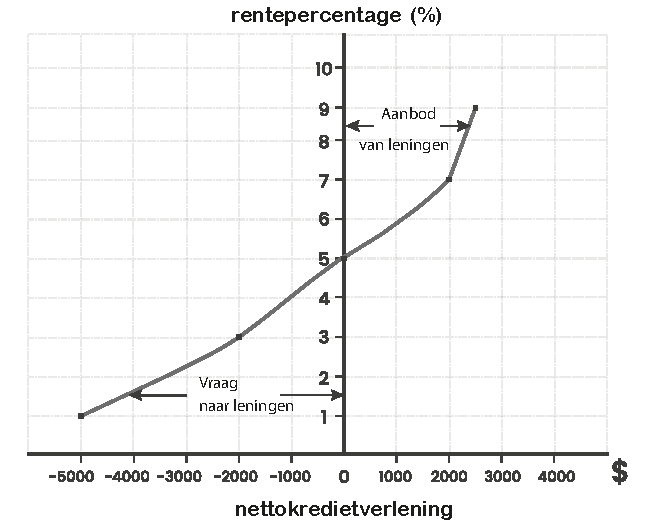
\includegraphics[width=0.9\textwidth]{figures/fig29.pdf}
    \caption[Persoonlijke tijdmarktcurve]{Persoonlijke tijdmarktcurve}
    \label{fig29}
\end{figure}

Op de kapitaalmarkt wordt de som van alle vraag- en aanbodcurven, in feite ieders individuele tijdsvoorkeur\index{tijdsvoorkeur}, samengevoegd tot algemene economische vraag- en aanbodcurven voor uitleenbare middelen. Bij elk gegeven rentetarief is er een totale hoeveelheid kapitaal\index{kapitaal} beschikbaar én gevraagd voor leningen. Aangezien het kapitaal\index{kapitaal} dat beschikbaar is voor leningen toeneemt naarmate de rente\index{rente} stijgt, terwijl het kapitaal\index{kapitaal} dat wordt gevraagd voor leningen afneemt naarmate de rente\index{rente} stijgt, zullen de twee elkaar maar één keer doorkruisen. Dit is het rentetarief dat de kapitaalmarkt in evenwicht brengt. Op dit punt zijn de hoeveelheid leningen perfect gelijk aan de hoeveelheid kapitaal\index{kapitaal} dat is onttrokken aan consumptie\index{consumptie} en beschikbaar is gesteld voor leners.

Het is belangrijk om nogmaals te benadrukken dat tijdsvoorkeur\index{tijdsvoorkeur} en de verdiscontering van de toekomst subjectieve verschijnselen zijn en dat ze niet worden gemeten aan de hand van rentepercentages. Wat er in de hoofden van handelende mensen gebeurt, is het maken van een ordinale rangorde van toekomstige en huidige goederen. Door te worden blootgesteld aan een aanbieding van een rentevoet zijn ze in staat om de impliciete verdiscontering die beschikbaar is op de markt ordinaal te vergelijken met hun persoonlijke verdiscontering en tussen de twee te kiezen. Verder bestaat er niet zoiets als een heersende marktrente. Er zijn alleen individuele rentepercentages die worden beïnvloed door de individuele projecten en de betrokken individuen. De marktrente kan, net als de marktevenwichtsprijs, vooral beschouwd worden als een hulpmiddel om deze economische concepten te begrijpen. Hoewel wiskundige analyse nuttig kan zijn om een begrip van marktverschijnselen over te brengen, is het belangrijk om niet in de val te lopen door ze te behandelen als wetenschappelijke eenheden gebaseerd op nauwkeurige metingen van constanten.

\begin{figure}
\centering
    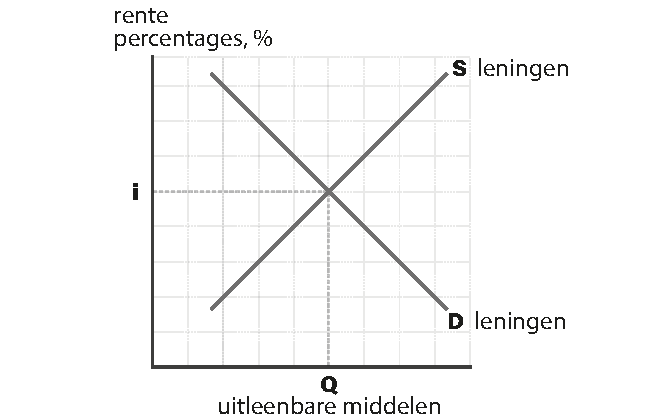
\includegraphics[width=0.7\textwidth]{figures/fig30.pdf}
    \caption[De markt voor leenbaar kapitaal\index{kapitaal}]{De markt voor leenbaar kapitaal\index{kapitaal}}
    \label{fig30}
\end{figure}

Naarmate meer kapitaal\index{kapitaal} wordt ingezet voor economische productie\index{productie}, neemt de productiviteit toe en stijgen de inkomens. Door goed beschermde eigendomsrechten en meer zekerheid over de toekomst zal de tijdsvoorkeur\index{tijdsvoorkeur} naar verwachting verder afnemen, waardoor mensen eerder geneigd zullen zijn om consumptie\index{consumptie} uit te stellen, meer zullen sparen, sneller geld zullen uitlenen en minder snel zelf zullen lenen. De overvloed aan leenbare middelen maakt de financiering mogelijk van een toenemend aantal productieve bedrijven tegen steeds lagere rentetarieven. Als dit proces niet wordt verstoord door oorlog\index{oorlog}, epidemieën, plunderingen, de perverse regeldruk van gecentraliseerde overheden of door met geweld opgedrongen zacht fiatgeld\index{fiatgeld}, zal deze opwaartse trend van toenemend materieel welzijn doorgaan. Dit kan worden beschouwd als het beschavingsproces. Maar hoe ver kan dit proces gaan? Hoe laag kan de rente\index{rente} gaan?

\hypertarget{kan-rente-worden-afgeschaft}{%
\section{Kan rente worden afgeschaft?}\label{kan-rente-worden-afgeschaft}}

Leningen met rente\index{rente} zijn op historisch, politiek en religieus vlak een beladen onderwerp. Veel religies verbieden ze en tot op de dag van vandaag worden ze door veel mensen wereldwijd als immoreel gezien, zelfs in een monetair systeem dat zwaar leunt op kredietcreatie. Mises en de Oostenrijkse economen hebben veel moeite gedaan om uit te leggen dat renteleningen een onlosmakelijk onderdeel van een markteconomie zijn. Ook beargumenteerden ze waarom het een productief element is in de markteconomie. Vanuit het perspectief van de Oostenrijkse economie is rente\index{rente} geen vreemde uitvinding die door leiders aan de maatschappij wordt opgelegd. Zoals alle economische fenomenen vindt rente\index{rente} zijn oorsprong in menselijk handelen\index{menselijk handelen} en in de tijdsvoorkeur\index{tijdsvoorkeur} die in elk individu positief is. Zoals Mises verwoordt:

\begin{blockquotebox}
We kunnen ons nauwelijks een wereld voorstellen waarin natuurlijke rente\index{rente} niet zou bestaan als een onmisbaar element in elke vorm van handelen ... Als er geen natuurlijke rente\index{rente} zou zijn, zouden kapitaalgoederen\index{kapitaalgoederen} niet worden besteed aan onmiddellijke consumptie\index{consumptie} en zou kapitaal\index{kapitaal} niet worden verbruikt. Integendeel, onder zo\textquotesingle n ondenkbare en onvoorstelbare stand van zaken zou er helemaal geen consumptie\index{consumptie} zijn maar alleen sparen, kapitaalopbouw en investeringen. Het is niet de onmogelijke verdwijning van natuurlijke rente\index{rente} die zou leiden tot kapitaalconsumptie, maar het afschaffen van rentebetalingen aan kapitaalbezitters. Juist omdat er natuurlijke rente\index{rente} is en het voldoen aan huidige behoeften de voorkeur heeft boven voldoening op een later tijdstip, zullen de kapitalisten hun kapitaalgoederen\index{kapitaalgoederen} en hun kapitaal\index{kapitaal} consumeren.\footnotemark
\end{blockquotebox}
\autocite{161}

Pogingen om rente\index{rente} af te schaffen zullen volgens Mises dus niet leiden tot de afschaffing van leningen tegen rente\index{rente} en zullen in plaats daarvan leiden tot de consumptie\index{consumptie} van kapitaalvoorraden omdat, wanneer ze er geen rendement op kunnen maken, spaarders minder gemotiveerd zijn om hun kapitaal\index{kapitaal} te behouden. Mensen verbieden om financiële activa te verhandelen op basis van hun tijdsvoorkeur\index{tijdsvoorkeur} zal hun tijdsvoorkeur\index{tijdsvoorkeur} niet elimineren, het zal altijd hun consumptie\index{consumptie}- en productiebeslissingen blijven beïnvloeden. Als kapitaalbezitters met een positieve tijdsvoorkeur\index{tijdsvoorkeur} geen toegang meer hebben tot de optie om tegen rente\index{rente} te lenen, zullen ze een sterkere prikkel hebben om hun kapitaalvoorraad te consumeren. Het verbieden van rente\index{rente} zorgt er dus voor dat de leners slechter af zijn, aangezien ze geen toegang meer zullen hebben tot broodnodige financiële middelen. Ook de kredietverstrekkers zijn slechter af omdat ze geen rendement meer kunnen halen uit hun spaargeld. Dit schaadt de maatschappij in zijn geheel door de stimulans om te sparen te verminderen, wat leidt tot minder kapitaalopbouw. Een maatschappij zonder rente\index{rente} op leningen is dus minder productief, minder innovatief en minder welvarend.

Vanuit Oostenrijks perspectief is het moeilijk om te beargumenteren dat rente\index{rente} de uitbuiting van de lener is. Er is geen dwang in het leencontract en beide partijen kiezen er vrijwillig voor om het aan te gaan, waardoor er geen wettelijke of morele rechtvaardiging is om het als illegaal te bestempelen, of om als derde partij met geweld te proberen te verhinderen dat de twee partijen transacties met elkaar aangaan.

\begin{blockquotebox}
Er kan daarom geen sprake zijn van het afschaffen van rente\index{rente} door instituten, wetten of bankmanipulatie. Wie rente\index{rente} wil ``afschaffen'' zal de mensen ertoe moeten brengen om een appel die over honderd jaar beschikbaar is niet minder te waarderen dan een appel in het heden. Wat afgeschaft kan worden door wetten en decreten is slechts het recht van de kapitalisten om rente\index{rente} te ontvangen. Zulke decreten zullen echter leiden tot kapitaalconsumptie waardoor de mensheid zeer snel zal terugvallen in de oorspronkelijke staat van natuurlijke armoede.\footnotemark
\end{blockquotebox}
\autocite{162}

De grootste breuk met de Oostenrijkse orthodoxie in dit boek is het argument waarom de rentevoet in feite kan worden geëlimineerd door een zuiver vrije markt en niet door officiële afschaffing of een decreet. Zoals besproken in het vorige hoofdstuk en in detail uitgelegd door Hoppe in \emph{Democracy}, wordt het beschavingsproces gestart met het verlagen van de tijdsvoorkeur\index{tijdsvoorkeur}, wat resulteert in kapitaalaccumulatie, verhoogde productiviteit en verbeterde levensstandaarden, die op hun beurt verdere daling van de tijdsvoorkeur\index{tijdsvoorkeur} aanmoedigen in een zich voortdurend versterkende spiraal. Oorlogen, ziekten, natuurrampen, toegenomen onzekerheid over de toekomst en groeiende onzekerheid over eigendomsrechten kunnen dit proces tegenhouden door een toename van de tijdsvoorkeur\index{tijdsvoorkeur} te veroorzaken en mensen te dwingen om steeds meer prioriteit te geven aan het heden ten koste van de toekomst.

De historische gegevens ondersteunen deze stelling. Zoals besproken in het vorige hoofdstuk, en zoals gedetailleerd beschreven in de encyclopedische studie over dit onderwerp door Homer en Sylla, heeft de mensheid de afgelopen 5000 jaar een gestage, langdurige daling van de rentetarieven gezien, onderbroken door de eerder genoemde calamiteiten.\autocite{163} Hoppe vat de geschiedenis van de rentedalingen als volgt samen:

\begin{blockquotebox}
    In feite kenmerkt een tendens van dalende rentetarieven de overkoepelende trend van de ontwikkeling van de mensheid. De minimumrente op ``normale veilige leningen'' lag aan het begin van de Griekse financiële geschiedenis in de zesde eeuw voor Christus rond de 16 procent en daalde tot 6 procent tijdens de Hellenistische periode. In Rome daalden ze van meer dan 8 procent tijdens de eerste periode van de Republiek tot 4 procent tijdens de eerste eeuw van het Keizerrijk. In het Europa van de dertiende eeuw was de laagste rente\index{rente} op ``veilige'' leningen 8 procent, waarna ze in de veertiende eeuw daalden tot ongeveer 5 procent. In de vijftiende eeuw daalden ze naar 4 procent, en in de zeventiende eeuw daalden ze naar 3 procent. Aan het einde van de negentiende eeuw waren de minimumrentes verder gedaald tot wel minder dan 2,5 procent.\footnotemark
\end{blockquotebox}
\autocite{164}

Toch werd deze trend van dalende rentetarieven in de twintigste eeuw tenietgedaan. Waarschijnlijk speelde de transitie naar fiatgeld\index{fiatgeld} een grote rol in deze verschuiving, samen met vele andere factoren die uitvoerig besproken worden in Hoppe\textquotesingle s \emph{Democracy}. Een hypothetisch gedachte-experiment dat hier interessant is, gaat als volgt: wat zou er gebeurd zijn met de rentetarieven als ze in de twintigste eeuw verder waren blijven dalen? Wat zou er zijn gebeurd als de wereld op een goudstandaard\index{goudstandaard} zou zijn gebleven en mensen de mogelijkheid zouden hebben behouden om voor de toekomst te sparen, kapitaal\index{kapitaal} nog overvloediger zou zijn geworden en de productiviteit verder zou zijn toegenomen? Hoe laag zouden de rentetarieven dan zijn geweest?

We kunnen de stelling van Mises dat de natuurlijke rente\index{rente} nooit tot nul kan dalen accepteren, en toch uitkomen op een marktrente van nul. Geld brengt namelijk, net als alle andere goederen, kosten met zich mee, bijvoorbeeld om het simpelweg te bewaren. Welke vorm het ook aanneemt, geld vereist bewaring en opslag, en dit zal altijd kosten met zich meebrengen die niet nul zijn en er zal altijd een risico\index{risico} van diefstal, verlies of schade aan vast hangen. Deze kosten kunnen op verschillende manieren worden betaald, zoals via de aankoop van een kluis of een opslagplaats, door de kosten van een depositorekening bij een bank\index{bank} of door het bedrag te verzekeren. Of er kan betaald worden in de vorm van diefstal en verlies, wat een risico\index{risico} is dat altijd bestaat. Er moeten bepaalde kosten, die niet nul zijn, worden betaald om geld te bewaren. De opportuniteitskosten van het uitlenen liggen voor de geldschieter niet in het volledig behouden van hun nominale rijkdom, maar niet uitlenen zal voor hem betekenen dat de waarde van het geld langzaam daalt door de kosten om het veilig te houden.

Als de tijdsvoorkeur\index{tijdsvoorkeur} samen met de natuurlijke rente\index{rente} blijft dalen, kan de marktrente uiteindelijk lager worden dan de bewaarkosten van het geld. In zo'n situatie zou de geldschieter graag geld uitlenen tegen een nominale rente\index{rente} van 0\%, omdat dit een beter rendement is dan het geld gewoon aan te houden, wat een negatief rendement zou betekenen. In plaats van rente\index{rente} per decreet af te schaffen, zou het voortdurende proces van beschaving\index{beschaving}, kapitaalaccumulatie en de daling van tijdsvoorkeur\index{tijdsvoorkeur} het lenen met rente\index{rente} op natuurlijke wijze volledig kunnen elimineren.

Een daling van de tijdsvoorkeur\index{tijdsvoorkeur} vergroot de overvloed aan kapitaal\index{kapitaal} en naarmate deze overvloed verder toeneemt, zal de prijs\index{prijs} van kapitaal\index{kapitaal}, in de vorm van rente\index{rente}, dalen. Een beschaving\index{beschaving} die voortdurend vooruitgang boekt, ervaart een daling van haar tijdsvoorkeur\index{tijdsvoorkeur}, wat leidt tot meer toekomstige voorzieningen en een groter moreel plichtsbesef met betrekking tot toekomstige generaties. Dit resulteert in een grote overvloed aan kapitaal\index{kapitaal}. Wanneer mensen in het bezit zijn van grotere hoeveelheden kapitaal\index{kapitaal}, neemt ook de vraag naar leningen af. Op dat moment kan een lener zich verzekeren van een lening\index{lening} van de vele beschikbare kredietverstrekkers door simpelweg te beloven om het geld volledig terug te betalen. Dit bespaart de kredietverstrekker namelijk de kosten van opslag en verzekering, of het risico\index{risico} op diefstal en verlies.

Naarmate de rente\index{rente} samen met de tijdsvoorkeur\index{tijdsvoorkeur} daalt, wordt de asymmetrie van de leenovereenkomst steeds onaantrekkelijker voor de kredietverstrekker. Waarom het risico\index{risico} nemen om al het kapitaal\index{kapitaal} te verliezen in ruil\index{ruil} voor zo\textquotesingle n mager rendement? Het leencontract beperkt het opwaartse voordeel voor de kredietverstrekker, maar er is geen enkele garantie dat de kredietverstrekker zijn geld echt terugkrijgt. Risico bestaat, en het risico\index{risico} van een volledig en catastrofaal verlies kan nooit volledig worden weggenomen. In het moderne, op fiat\index{fiat} gebaseerde economische systeem, is het faillissementsrisico van banken sterk verminderd door het risico\index{risico} over te dragen naar de nationale valuta zelf. Leningen worden in feite gegarandeerd door de mogelijkheid van de centrale bank\index{centrale bank} om de kredietverstrekkers schadeloos te stellen bij eventuele wanbetalingen op hun portfolio. Dit is de reden waarom de FDIC (Federal Deposit Insurance Corporation) in staat is om bankrekeningen in de moderne wereld te garanderen, maar in de hypothetische samenleving van dit scenario is dit niet iets waarvan je zou verwachten dat het bestaat. Kapitaalaccumulatie en een daling van de tijdsvoorkeur\index{tijdsvoorkeur} zouden niet vergevorderd kunnen zijn in een samenleving met inflatoir fiatgeld\index{fiatgeld} dat door de centrale bank\index{centrale bank} gebruikt kan worden om banken te redden, omdat dergelijk geld het sparen zou ontmoedigen en het niet zou toelaten dat de tijdsvoorkeur\index{tijdsvoorkeur} en rentetarieven dalen. We zouden zo\textquotesingle n punt alleen kunnen bereiken met een harde geldstandaard die sparen aanmoedigt en die banksteun of faillissementsbescherming voor kredietverstrekkers uitsluit. In zo\textquotesingle n wereld van lage tijdsvoorkeur\index{lage tijdsvoorkeur}, hard geld\index{hard geld} en zonder financiële reddingsoperaties wordt lenen tegen rente\index{rente} onwaarschijnlijk. Kredietverstrekkers zouden een zeer klein rendement behalen, terwijl het volledige bedrag in rook op kan gaan. Als ze het volledige risico\index{risico} op zich nemen, zouden ze liever ook meegenieten van de winsten via een investering in aandelen.

In een wereld van grote overvloed aan kapitaal\index{kapitaal}, verwaarloosbaar lage rentes, of zelfs rentetarieven van nul procent, zullen mensen die kredietwaardig zijn geen probleem hebben om kapitaal\index{kapitaal} van vrienden en familie te lenen in geval van nooduitgaven of tegenspoed. Uitlenen zonder rente\index{rente} bespaart de eigenaar van het geld de noodzaak om geld uit te geven aan opslag en verlost hem van het risico\index{risico} van verlies. Bij een zeer lage tijdsvoorkeur\index{lage tijdsvoorkeur} is uitlenen aan een vertrouwde lener dus voordeliger dan het geld zelf aanhouden. Voor zakelijke investeringen is het echter waarschijnlijker dat de markt zich voornamelijk zal richten op aandelen. In een dergelijke wereld zal het bankwezen netjes worden opgedeeld in twee categorieën: investeringsbanken en depositobanken.

De hierboven besproken gouden regel van Mises stelt dat goederenkrediet volledig moet worden gedekt door spaargeld met dezelfde looptijd van de lening\index{lening}. Maar zonder een mogelijke ultieme geldschieter (of: \emph{lender of last resort}) en bij een nominale rente\index{rente} van nul, zal deze regel een extra bepaling krijgen: de kredietverlener krijgt een vooraf overeengekomen aandeel in de winst van de onderneming. Met andere woorden, er zal geen kredietverstrekker zijn, maar een investeerder met eigen vermogen in de onderneming.

Inzicht in de tijdsvoorkeurtheorie van rentetarieven vanuit het Oostenrijkse perspectief, ook wel bekend als de agiotheorie, kan helpen om de historische en religieuze argumenten tegen rente\index{rente} te verklaren. In een wereld waarin de nominale rentevoet nul is, is de tijdsvoorkeur\index{tijdsvoorkeur} zo laag dat de natuurlijke rente\index{rente} lager is dan de bewaarkosten van geld. Religieuze mandaten tegen rente\index{rente} kunnen worden beschouwd als instructies voor de religieuzen om hun tijdsvoorkeur\index{tijdsvoorkeur} te verlagen tot het punt waarop het lenen met rente\index{rente} voor hen niet meer aantrekkelijk is. Geloof in het hiernamaals kan mogelijk bevorderlijk werken voor het verlagen van de tijdsvoorkeur\index{tijdsvoorkeur}. Verwachtingen om tot in de eeuwigheid te leven, en dus oneindig veel beloningen en straffen voor hun daden te ervaren, zouden kunnen leiden tot een oneindig lage afwaardering van toekomstige gevolgen.

Terwijl religies en tradities deze realiteit aan hun gelovigen proberen op te leggen door middel van leefregels, is de moderne markteconomie het instrument dat ons in de praktijk naar deze realiteit stuurt, allemaal door middel van constante kapitaalaccumulatie, arbeidsdeling\index{arbeidsdeling}, technologische vooruitgang en het verlagen van tijdsvoorkeur\index{tijdsvoorkeur}. Met andere woorden, als de processen van de markt en de beschaving\index{beschaving} ononderbroken doorgaan, neemt het verdisconteren van de toekomst af tot het punt waarop rente\index{rente} wordt geëlimineerd. Dit resulteert in een systeem zonder woekerrente, vergelijkbaar met het traditionele christelijke en islamitische bankieren.

Joseph Schumpeter geeft een goede samenvatting van het werk van Eugene Böhm-Bawerk, de Oostenrijkse econoom die het meest bijdroeg aan de ontwikkeling van de Oostenrijkse rentetheorie.

\begin{blockquotebox}
    {[}Rente{]} is als het ware de rem of de regelaar die individuen ervan weerhoudt de economisch\index{economisch} toelaatbare verlenging van de productieperiode te overschrijden en die voorzieningen voor huidige behoeften afdwingt -- wat in feite hun urgentie onder de aandacht van ondernemers brengt. Het weerspiegelt daardoor de relatieve intensiteit waarmee in elke economie toekomstige en huidige belangen zich doen gelden, en dus ook de intelligentie en de morele kracht van een volk -- hoe hoger deze zijn, hoe lager de rentevoet zal zijn. Daarom weerspiegelt de rentevoet het culturele niveau van een natie; want hoe hoger dit niveau, hoe groter de beschikbare voorraad consumptiegoederen\index{consumptiegoed}, hoe langer de productieperiode, hoe kleiner, volgens de wet van de afnemende opbrengst, de meeropbrengst die verdere verlenging van de productieperiode zou opleveren, en dus hoe lager de rentevoet. En hier hebben we Böhm-Bawerk\textquotesingle s wet van de dalende rente\index{rente}, zijn oplossing voor dit oude probleem waarover de slimste koppen van onze wetenschap zonder succes het hoofd hebben gebroken.\footnotemark
\end{blockquotebox}
\autocite{165}

Of een voortdurende daling van de tijdsvoorkeur\index{tijdsvoorkeur} de rentetarieven echt zal doen dalen tot een nominaal nultarief is een vraag die losstaat van de economische doeltreffendheid van een dwingend verbod op rente\index{rente}. Zonder de vereiste lage tijdsvoorkeur\index{lage tijdsvoorkeur} zal het verbieden van renteleningen waarschijnlijk leiden tot meer consumptie\index{consumptie}, minder sparen en uitlenen, en waarschijnlijk minder investeringen in het algemeen. Het is mogelijk dat lenen tegen rentes het enige is dat de rentelening kan laten verdwijnen. Door sparen te stimuleren en kapitaalaccumulatie te vergroten, leidt de rentelening tot een daling van de tijdsvoorkeur\index{tijdsvoorkeur} en rentetarieven, tot ze uiteindelijk compleet verdwijnen.

\hypertarget{monetaire-expansie}{%
\chapter{Monetaire Expansie}\label{monetaire-expansie}}

\begin{blockquotebox}
    Kredietexpansie kan kapitaal\index{kapitaal} niet vervangen.\footnotemark
    \par\raggedleft--- Ludwig von Mises\index{Ludwig von Mises}
\end{blockquotebox}
\autocite{166}

\vspace{-1em}
\hypertarget{circulatiekrediet}{%
\section{Circulatiekrediet}\label{circulatiekrediet}}

\lettrine{I}n het vorige hoofdstuk werd uitgelegd hoe goederenkrediet werkt, dat Mises definieert als krediet\index{krediet} dat door banken wordt verstrekt met een perfecte overeenstemming tussen de omvang en de looptijd van de lening\index{lening} van de spaarders aan de bank\index{bank}, en van de bank\index{bank} aan de investeerders. Met andere woorden, goederenkrediet is een krediettransactie waarbij de bank\index{bank} slechts een tussenpersoon is die de afstemming tussen spaarders en investeerders vergemakkelijkt. In elke transactie van goederenkrediet leidt het bedrag van het geïnvesteerde kapitaal\index{kapitaal} tot een uitstel van consumptie\index{consumptie} door de eigenaren van het geïnvesteerde spaargeld voor een gelijk bedrag, wat betekent dat rentetarieven de tijdsvoorkeur\index{tijdsvoorkeur} van de kredietverstrekker weerspiegelen. Dit hoofdstuk gaat over kredietregelingen waarin een investering niet leidt tot een afname van de consumptie\index{consumptie} door de kredietverstrekkers. Volgens wat Mises benoemt als circulatiekrediet, resulteert lenen in de creatie van nieuw geld.

De meest voorkomende manier waarop circulatiekrediet ontstaat, is wanneer financiële instellingen geld uitlenen waarvan ze tegelijkertijd beloven dat het beschikbaar is voor de spaarder. Dit staat in de praktijk ook wel bekend als \textbf{fractioneel bankieren\index{fractioneel bankieren}}. De uitlener, in dit geval de depositohouder van de bank\index{bank}, hoeft de consumptie\index{consumptie} van zijn deposito niet uit te stellen, terwijl het wordt uitgeleend als krediet\index{krediet} aan een ondernemer, zoals het geval is bij goederenkrediet waarbij de spaarder gedurende de hele looptijd van de lening\index{lening} aan de ondernemer afstand doet van zijn deposito. Dit laatste wordt ook wel ``full reserve, maturity matched commodity credit'' genoemd.

Een andere manier waarop een bank\index{bank} circulatiekrediet kan creëren is door de looptijden van haar leningen en deposito\textquotesingle s niet op elkaar af te stemmen. Als de bank\index{bank} alleen krediet\index{krediet} uitleent voor een bedrag gelijk aan haar deposito\textquotesingle s, maar dit ook uitleent met een langere looptijd dan ze heeft geleend, dan creëert ze ook circulatiekrediet. De lening\index{lening} gaat er in feite van uit dat de bank\index{bank} nieuwe depositohouders zal kunnen vinden die bereid zijn geld te storten tegen een lagere rente\index{rente} dan de rente\index{rente} die ze aan de ondernemer biedt. Elke keer wanneer de gouden regel die in Hoofdstuk 14 werd besproken wordt overtreden, komt er dus meer circulatiekrediet in omloop.

Een derde manier waarop circulatiekrediet kan worden gecreëerd is door herhypothecatie van onderpand voor leningen -- het hergebruik van onderpand voor meer dan één lening\index{lening}. Als het onderpand al eerder was verpand voor een lening\index{lening}, dan betekent de tweede lening\index{lening} geen uitstel van consumptie\index{consumptie} voor de kredietverstrekker.

Op al deze drie manieren wordt er krediet\index{krediet} gecreëerd zonder evenredige opoffering van de kant van de kredietverstrekker. Het wordt uitgegeven als \textbf{fiduciaire middelen}: bankbiljetten\index{bankbiljetten} en banksaldi die inwisselbaar zijn voor geld, maar waarvan geen gelijkwaardige geldhoeveelheid beschikbaar is om uitbetaald te worden door de bank\index{bank} wanneer de depositotermijn verloopt.

Geld is, zoals besproken in Hoofdstuk 10, uniek omdat het het enige goed is dat uitsluitend wordt verkregen om weer te worden geruild voor iets anders. Het wordt niet geconsumeerd, zoals consumptiegoederen\index{consumptiegoed}, noch gebruikt bij de productie\index{productie} van andere goederen, zoals kapitaalgoederen\index{kapitaalgoederen}. Aangezien de enige functie van geld is om het om te ruilen en het verder geen fysieke functie heeft voor de eigenaar, kan een vordering erop, of een substituut ervoor, dezelfde rol vervullen terwijl dit niet het geval is voor een substituut of vordering op een ander consumptiegoed\index{consumptiegoed} of kapitaalgoed\index{kapitaalgoederen}. Een coupon voor een biefstuk kan niet worden opgegeten, een coupon voor een machine kan geen goederen produceren, en met een vliegticket kun je niet vliegen. Een vordering op geld kan echter wel de essentiële functie van geld vervullen: het kan worden geruild voor andere goederen. In de woorden van Mises:

\begin{blockquotebox}
    De bijzondere houding van mensen ten aanzien van transacties waarbij circulatiekrediet betrokken is, is te verklaren doordat vorderingen op geld kunnen worden gebruikt voor alle transacties, in plaats van geld zelf. Wie geld nodig heeft, om het uit te lenen, om iets te kopen, om schulden te vereffenen, of om belastingen te betalen, is niet eerst verplicht om de geldvorderingen (biljetten of banktegoeden) om te zetten in geld; de vorderingen zelf kunnen ook direct gebruikt worden als betaalmiddel. Ze zijn dus eigenlijk geldsubstituten; ze vervullen de monetaire functie op dezelfde manier als geld; het is in feite contant geld\index{contant geld} dat direct kan worden uitgegeven, en geen geld dat pas in toekomst beschikbaar wordt.
    \par\vspace{1em}\noindent
    Iemand die duizend broden bezit, zal niet meer dan duizend coupons uitgeven die elke bezitter het recht geven om te allen tijde een brood op te eisen. Met geld ligt dit anders. Omdat niemand geld op zich waardeert, maar het slechts wenst te gebruiken als ruilmiddel voor iets anders, is het zeer wel mogelijk dat er schuldbewijzen voor in de plaats komen. Deze schuldbewijzen kunnen van hand tot hand gaan zonder dat iemand daadwerkelijk probeert het ermee verbonden recht op te eisen.\footnotemark
\end{blockquotebox}
\autocite{167}

Door hun unieke eigenschappen kunnen fiduciaire middelen, zoals bankbiljetten en bankrekeningen die door de bank\index{bank} zijn uitgegeven, als geld functioneren. Ze kunnen worden gebruikt voor de aankoop van goederen of diensten en als betaling worden geaccepteerd zonder dat ze bij de uitgevende bank\index{bank} ingewisseld moeten worden voor contant geld. Deze fiduciaire middelen dienen als ruilmiddel\index{ruilmiddel}, zonder ze om te moeten zetten in geld. Belangrijk is dat fiduciaire middelen fundamenteel verschillen van bankbiljetten\index{bankbiljetten} die volledig gedekt zijn door contanten, die de bank\index{bank} op verzoek beschikbaar heeft: de uitgifte van fiduciaire middelen vergt geen opoffering van de kant van de uitgever. Wanneer bankbiljetten\index{bankbiljetten} worden uitgegeven met een 100\% dekking, blijft de totale geldhoeveelheid ongewijzigd. Echter, bij de uitgifte van fiduciaire middelen neemt de geldvoorraad toe. Terwijl het delven van goud\index{goud} een kostbare en onzekere activiteit is, waarvan de kosten vaak in de buurt komen van de verwachte opbrengst van het goud\index{goud}, brengt de uitgifte van fiduciaire middelen een uitbreiding van de geldvoorraad met zich mee zonder significante kosten voor de uitgevende bank. Deze toename van de geldhoeveelheid heeft natuurlijk invloed op de marktwaarde van geld, met verstrekkende gevolgen die door de Oostenrijkse School\index{Oostenrijkse School} al meer dan een eeuw zorgvuldig worden geanalyseerd, en die in de volgende secties worden besproken.

\hypertarget{mises-typologie-van-geld}{%
\section{Mises\textquotesingle{} typologie van geld}\label{mises-typologie-van-geld}}

Door de bijzondere aard van geld, als een goed dat niet geconsumeerd wordt, kunnen geldsubstituten en fiduciaire middelen evengoed een monetaire rol spelen als geld zelf, waardoor verwarring kan ontstaan over wat er precies bedoeld wordt met de term ``geld''. Er bestaat een belangrijk onderscheid en het is daarom nuttig om de typologie te volgen die Mises uiteenzette in \emph{The Theory of Money and Credit} en die wordt uitgelegd in \emph{Mises: The Last Knight of Liberalism},\autocite{169} de intellectuele biografie van Mises door Jörg Guido Hülsmann:

\begin{blockquotebox}
    Mises ontwikkelde een uitgebreide typologie van monetaire objecten -- in Mengeriaanse taal kunnen we dit verwoorden als alle dingen die algemeen aanvaard worden als ruilmiddelen. Op het meest fundamentele niveau maakte hij een onderscheid tussen verschillende soorten ``geld in de nauwe zin'' en ``geldsurrogaten of --substituten''. Geld in nauwe zin is een goed op zichzelf, terwijl geldsubstituten daarentegen wettelijke vorderingen zijn op geld in nauwe zin. Ze worden meestal uitgegeven door banken en zijn terugbetaalbaar in echt geld aan de loketten van de bank\index{bank} die ze uitgeeft.
    \par\vspace{1em}\noindent
    Bij het vaststellen van dit fundamentele onderscheid tussen geld en geldvorderingen paste hij cruciale inzichten toe van Böhm-Bawerk\textquotesingle s baanbrekende werk over de economie van rechtspersonen. Hij benadrukte: ``Vorderingen zijn geen goederen; het zijn middelen om beschikking te krijgen over goederen. Dit kenmerkt hun hele aard en economische betekenis.'' Zoals zijn uiteenzetting in latere delen van het boek zou laten zien, is dit onderscheid van groot belang, zowel voor de integratie van de monetaire theorie binnen het kader van Mengers theorie van waarde en prijzen, als voor de analyse van de rol van het bankwezen binnen het monetaire systeem. De kern van zijn theorie over bankieren is een vergelijkende analyse van de economische betekenis van twee zeer verschillende soorten geldsubstituten. Mises merkte op dat geldsubstituten ofwel gedekt kunnen zijn door een overeenkomstige geldhoeveelheid, in welk geval ze ``geldcertificaten'' zijn, of ze kunnen een dergelijke dekking missen, in welk geval ze fiduciaire middelen of ``Umlaufsmittel'' zijn. Mises wijdt het derde en laatste deel van zijn boek aan een analyse van de economische gevolgen van het gebruik van Umlaufsmittel.\footnotemark
\end{blockquotebox}
\autocite{170}

De term ``geld'' wordt in brede kring gebruikt om te verwijzen naar zowel geld als geldsubstituten. Mises verduidelijkt het onderscheid op een manier die de Oostenrijkse analyse van de conjunctuurcyclus\index{conjunctuurcyclus} helpt verklaren. Geld, in de nauwere zin, kan drie vormen aannemen:

\vspace{1em}\noindent\textbf{Goederengeld}: Een algemeen ruilmiddel\index{ruilmiddel} dat ook een economisch\index{economisch} goed is en kan worden geruild met goederen van hetzelfde type. Het wordt verkocht op een open markt met veel producenten en consumenten. Historische voorbeelden zijn voornamelijk edelmetalen, maar recentelijk kan bitcoin\index{bitcoin} worden toegevoegd als een nieuwe vorm van een niet-metaal digitaal\index{digitaal} goed.

\vspace{1em}\noindent\textbf{Kredietgeld}: Een toekomstige financiële vordering op een rechtspersoon die wordt gebruikt als ruilmiddel\index{ruilmiddel}. Wat kredietgeld onderscheidt van krediet\index{krediet}, is dat de ontvanger het accepteert met de bedoeling het door te geven aan een andere ontvanger, niet omdat hij de financiële vordering wil innen.

\vspace{1em}\noindent\textbf{Fiatgeld}: Een ruilmiddel\index{ruilmiddel} dat geaccepteerd wordt op basis van een wettelijk besluit van een autoriteit. ``De beslissende factor is de stempel van de overheid\index{overheid}. Het is niet het materiaal dat de stempel draagt dat het geld vormt, maar de stempel zelf.''\autocite{171} Fiatgeld kan de vorm aannemen van papiergeld, bankdeposito\textquotesingle s of munten\index{munten}.

\vspace{1em}\noindent Hoewel geldsubstituten vaak met echt geld worden verward, zijn ze in feite verschillend.

\vspace{1em}\noindent\textbf{Geldsubstituten}: Fysieke of financiële instrumenten die wettige vorderingen zijn van geld in nauwe zin. Ze kunnen op verzoek worden ingewisseld voor geld en worden gebruikt als ruilmiddel\index{ruilmiddel} bij transacties. Geldsubstituten zijn er in twee vormen:

\vspace{1em}\noindent\textbf{Geldcertificaten}: Een financieel instrument of papier dat op verzoek volledig inwisselbaar is voor geld (de waarde wordt 100\% gedekt door de uitgevende instantie.) Voorbeelden zijn een dollarbiljet dat in goud\index{goud} kan worden ingewisseld onder een strikte goudstandaard\index{goudstandaard}, of een bankrekening gebaseerd op dollars met goud\index{goud} als onderpand. Op het gebied van bitcoin\index{bitcoin} kunnen we bitcoin\index{bitcoin} op het lightningnetwerk beschouwen als een uniek type geldcertificaat, omdat de werking ervan volledig in handen is van de houder van het geld en de terugbetaling niet afhankelijk is van derden. Verhandelbare eigendomsbewijzen voor bitcoin\index{bitcoin} die door een derde partij in bewaring worden gehouden zouden ook geldcertificaten zijn. En hoewel deze een tegenpartij zouden hebben die het uitgeeft, zouden ze nog steeds relatief goedkoop en gemakkelijk inwisselbaar zijn voor bitcoin\index{bitcoin}, omdat toegang tot het netwerk niet gemakkelijk te censureren is.

\vspace{1em}\noindent\textbf{Fiduciaire middelen}: Geldsubstituten die niet gedekt worden door een onderpand. Wanneer een financiële instelling geldsubstituten uitgeeft, maar niet het geld heeft om alle substituten terug te betalen, is er sprake van fiduciaire middelen. Dit is een sleutelterm in Mises\textquotesingle{} uitleg van de conjunctuurcyclus\index{conjunctuurcyclus}, want het is precies de creatie van deze middelen die de conjunctuurcyclus\index{conjunctuurcyclus} in gang zet. In het digitale domein zou dit het equivalent zijn van krediet\index{krediet}, uitgedrukt in bitcoin\index{bitcoin}, maar dat wordt uitgegeven zonder het equivalent aan bitcoin\index{bitcoin} als dekking.

\begin{figure}[H]
\centering
    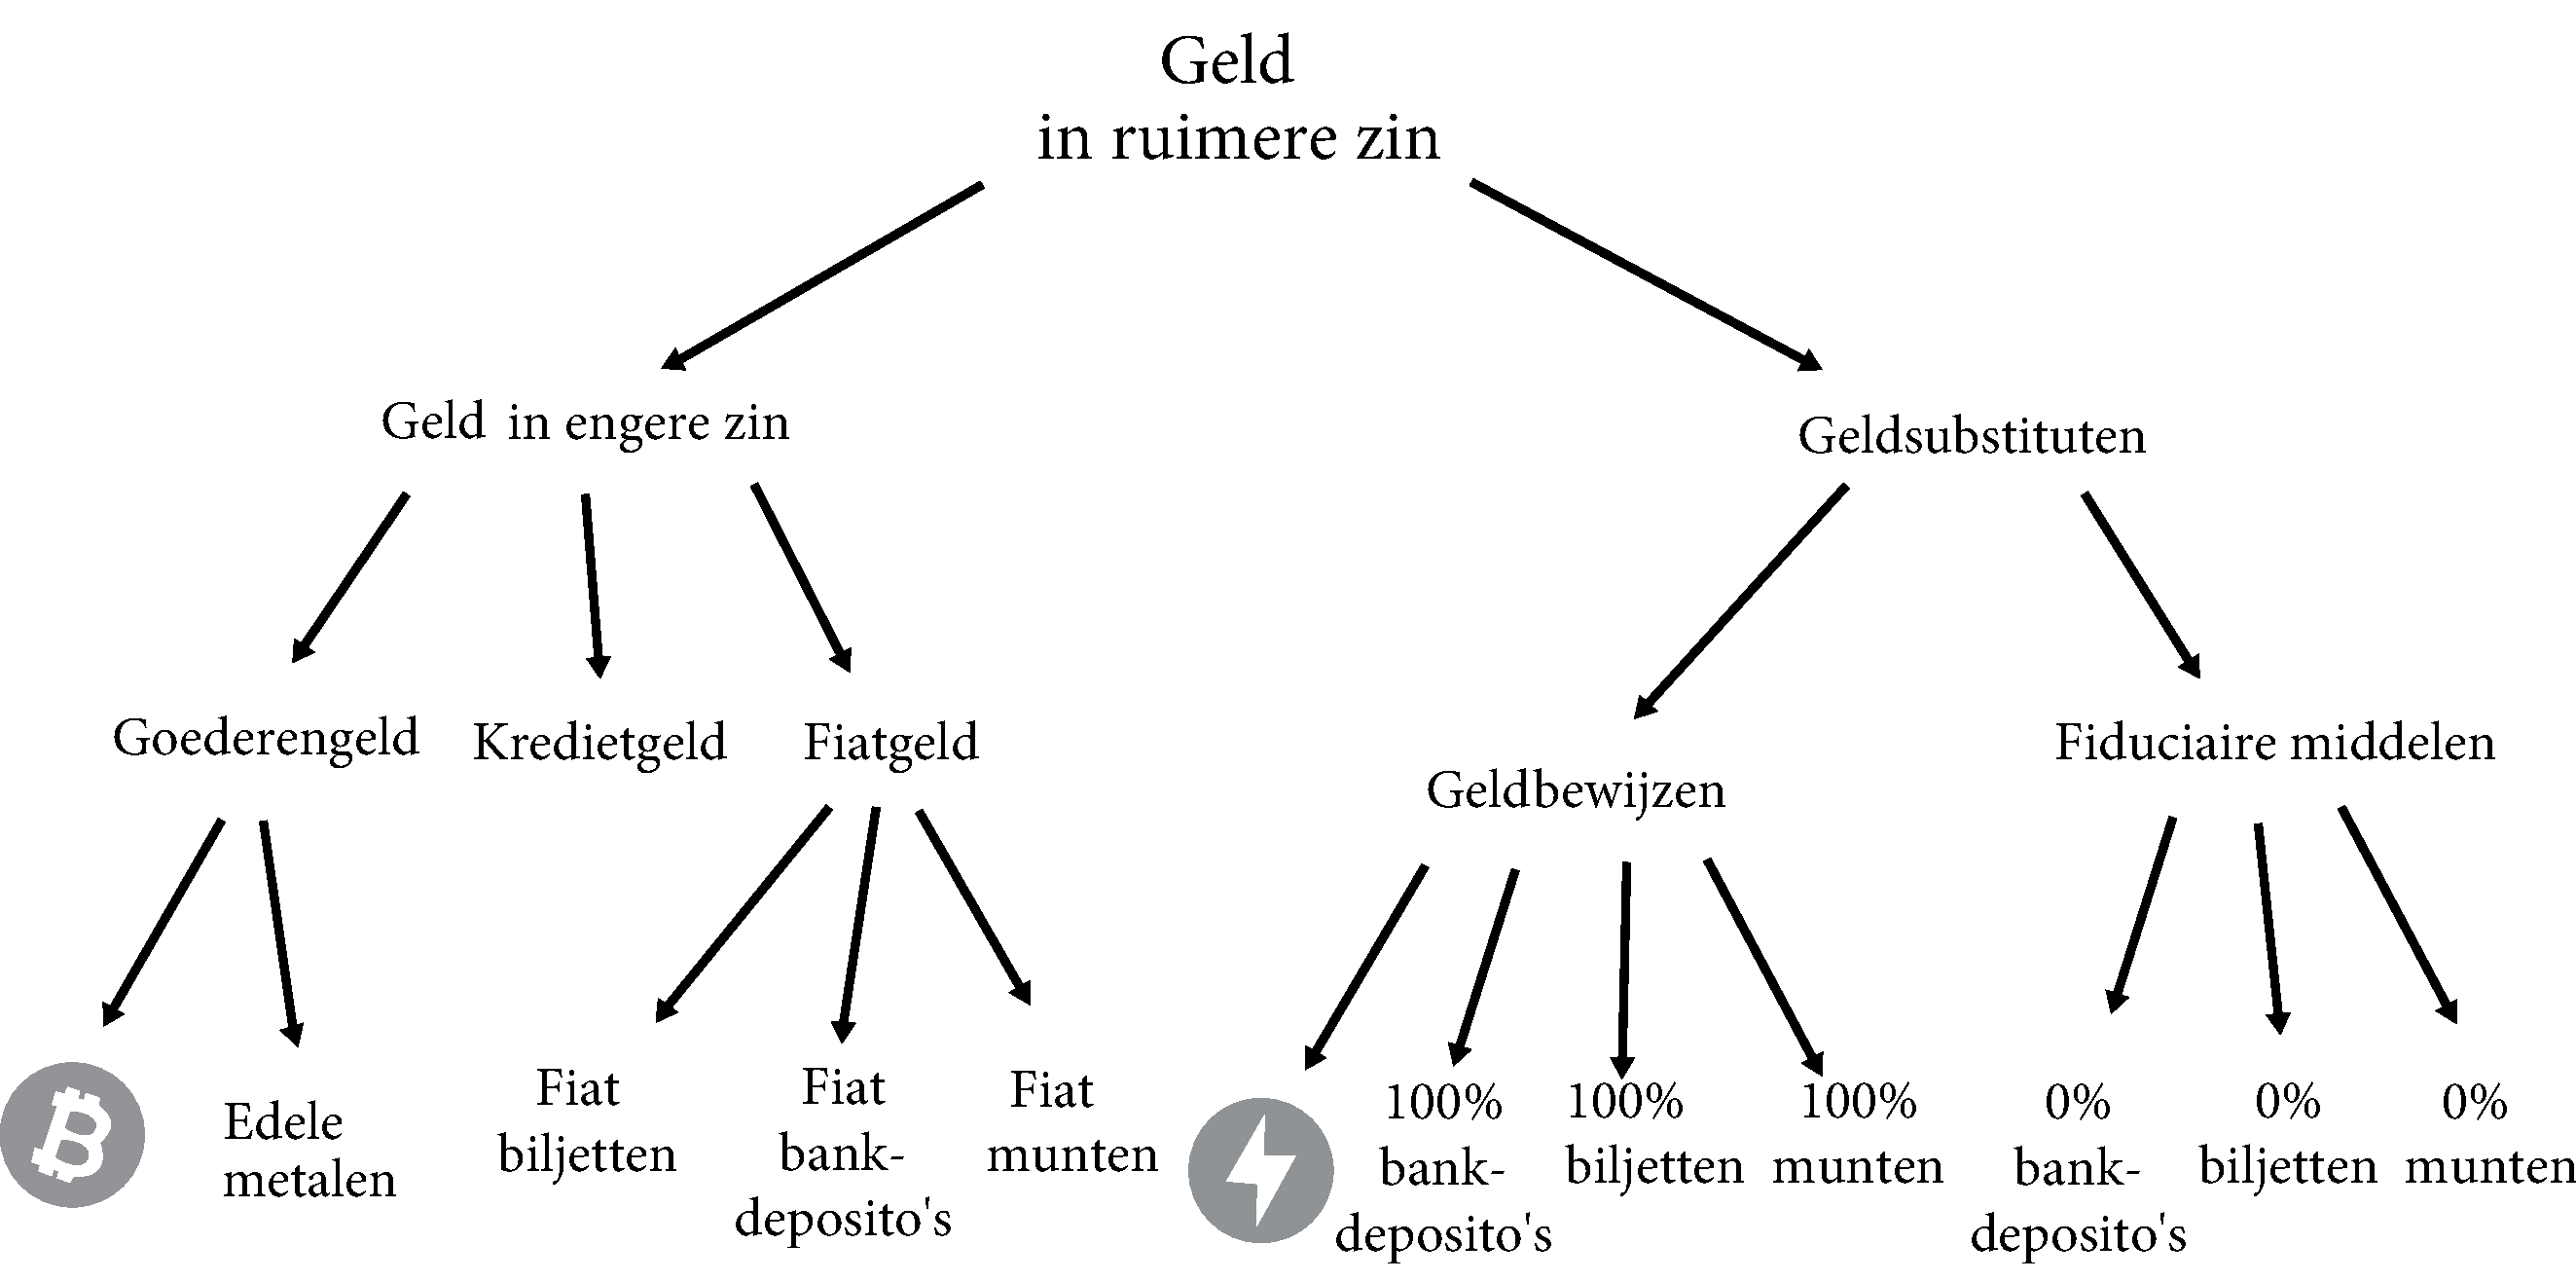
\includegraphics[width=\textwidth]{figures/fig31.pdf}
    \caption[Typologie van geld]{Typologie van geld\footnotemark}
    \label{fig31}
\end{figure}
\autocite{172}

Volgens de typologie van Mises staat de functie van geld los van zijn fysieke verschijning. Bankdeposito\textquotesingle s nemen de vorm van geldcertificaten aan wanneer ze volledig terugbetaalbaar zijn voor geld, van fiduciaire middelen wanneer ze uitgegeven worden door banken zonder dat er een onderpand tegenover staat, of van fiatgeld\index{fiatgeld} wanneer ze worden door de overheid\index{overheid} worden opgelegd. Volgens hetzelfde principe kan papiergeld een volledig gedekt geldcertificaat zijn en dus inwisselbaar zijn voor het onderliggende goederengeld tegen de nominale waarde, zoals dit was onder de goudstandaard\index{goudstandaard}. Als het echter uitgegeven wordt door een bank\index{bank} en niet terugbetaalbaar is voor geld, dan is het fiduciair geld; en het is fiatgeld\index{fiatgeld} als het gedrukt wordt door een overheid\index{overheid} zonder dat terugbetaling mogelijk is. Fysieke munten\index{munten} kunnen worden gemaakt als goederengeld, zoals gouden en zilveren munten\index{munten}; als fiduciaire middelen wanneer ze worden uitgegeven door een bank\index{bank}; als een geldcertificaat als het inwisselbaar is voor geld; of als fiatgeld\index{fiatgeld} als het wordt geslagen uit een basismetaal en de waarde onafhankelijk van het metaalgehalte wordt bepaald door een autoriteit. Door afstand te nemen van de fysieke verschijningsvormen van het geld en het verschil uit te leggen tussen fiduciaire middelen en geldcertificaten, kon Mises een verklaring geven voor het ontstaan van conjunctuurcycli op basis van menselijk handelen\index{menselijk handelen}.

Bij geldcertificaten is een gelijk bedrag aan geld in de nauwe zin opeisbaar door de houder bij de uitgevende instelling geplaatst; de uitgifte ervan veroorzaakt geen toename van de monetaire middelen in omloop. Wanneer het geldcertificaat op een bepaald moment voor een betaling wordt gebruikt, blijft het geld als dekking in een bankkluis liggen, maar verandert in feite van eigenaar. Dat geld kan geen monetaire transacties afwikkelen, terwijl de geldcertificaten in omloop zijn. Zodra het geldcertificaat is ingewisseld voor het geld in engere zin, kan het worden uitgegeven, maar het bewijs niet meer. Geldcertificaten vergroten de geldhoeveelheid in ruimere zin niet. De introductie van geldsubstituten in de vorm van fiduciaire middelen resulteert daarentegen wel in een toename van de totale geldhoeveelheid en geldsubstituten die in omloop zijn.

In het verleden verrijkten koningen zichzelf ten koste van hun volk door munten\index{munten} van hun onderdanen te verzamelen, het edelmetaalgehalte te verlagen door er onedele metalen in te vermengen, en vervolgens de munten\index{munten} opnieuw te slaan. Door onedele metalen aan de mix toe te voegen, kon de koning meer munten\index{munten} maken dan de hoeveelheid edelmetaal die hij had. Hierdoor kreeg hij zelf meer koopkracht ten koste van de eigenaars van de oorspronkelijke munt. Na verloop van tijd zou de prijs\index{prijs} van goederen stijgen als weerspiegeling van de daling van het edelmetaalgehalte. Een deel van ieders werkelijke rijkdom werd dus overgedragen aan de koning.

Hoewel moderne gecentraliseerde overheden hun fysieke munten\index{munten} niet langer ontwaarden, bereiken ze toch iets vergelijkbaars door wetgeving, dreiging met geweld en door hun monopoliemacht te gebruiken om mensen te dwingen om geldcertificaten die niet langer in geld kunnen worden terugbetaald te accepteren alsof het geld is. Nu ze niet meer inwisselbaar zijn, worden de geldcertificaten fiduciaire middelen, waardoor de totale geldhoeveelheid toeneemt. Op dezelfde manier waarop koningen profiteerden van het mengen van onedele metalen met edele metalen, profiteren moderne overheden van het mengen van fiduciaire middelen met geld. De gevolgen gaan in beide gevallen verder dan alleen het verrijken van de overheid\index{overheid} ten koste van de samenleving. Het introduceren van een goedkope aanvulling op het geld verbetert de functie ervan niet; het brengt het in gevaar. Geld onderscheidt zich van andere goederen doordat de absolute hoeveelheid niet van belang is voor de eigenaar, alleen de koopkracht doet er toe. Het verhogen van de geldhoeveelheid vergroot het vermogen niet, noch maakt het het geld effectiever; in plaats daarvan devalueert het de rijkdom van de huidige eigenaars en draagt het over aan de ontvangers van het nieuw gecreëerde geld. Het zal de prijzen van goederen veranderen waardoor uiteindelijk economische miscalculaties zullen ontstaan.

\hypertarget{conjunctuurcycli}{%
\section{Conjunctuurcycli}\label{conjunctuurcycli}}

De gangbare economische stromingen zijn uiterst voorzichtig bij het beantwoorden van de vraag wat de oorzaak is van conjunctuurcycli, en daar is een goede reden voor. Aangezien de moderne economische wetenschap grotendeels door centrale banken wordt gefinancierd om informatie voor beleidsvorming te leveren, is het erg onwaarschijnlijk dat iemand wiens conclusies niet vleiend zijn voor centrale banken een succesvolle carrière kan verwachten.\autocite{173} Mainstream economisch\index{economisch} onderzoek heeft zich voornamelijk gericht op discussies over hoe recessies kunnen worden voorkomen en gaf daarbij zeer weinig aandacht voor wat recessies eigenlijk veroorzaakt. Het is kinderachtig om te proberen een probleem op te lossen zonder de oorzaken ervan te begrijpen, maar met fiatgeld\index{fiatgeld} kunnen centrale banken proberen hun eigen realiteit te creëren. Dit doen ze door onderzoek te financieren dat gericht is op het vinden van oplossingen en door wetenschappers die kritisch staan tegenover centrale banken te marginaliseren. Deze benadering werd het best geïllustreerd in Krugmans inleiding op een recente herdruk van Keynes\textquotesingle{} \emph{General Theory}, waarin Krugman het onvermogen van Keynes om een verklaring te bieden voor de oorzaken van de conjunctuurcyclus\index{conjunctuurcyclus} prijst:

\begin{blockquotebox}
    In plaats van zich te verliezen in een poging om de dynamiek van de conjunctuurcyclus\index{conjunctuurcyclus} te verklaren -- een onderwerp dat tot op de dag van vandaag omstreden blijft -- richtte Keynes zich op een vraag die beantwoord kon worden. En die ... het hardst een antwoord nodig had: hoe kunnen we dan meer werkgelegenheid creëren als de algemene vraag laag is -- ongeacht de oorzaak?\footnotemark
\end{blockquotebox}
\autocite{174}

Om succesvol te zijn in de moderne academische wereld is het vooral vereist om loyaal te zijn aan de centrale banken, in plaats van de coherentie of de waarde van je ideeën. Als gevolg daarvan wordt de conjunctuurcyclus\index{conjunctuurcyclus} nog steeds voorgesteld als een normaal, onvermijdelijk onderdeel van de werking van een moderne kapitalistische economie. Het zou net zo onvermijdelijk zijn als de overgang van dag naar nacht.

In schril contrast hiermee bieden de Oostenrijkse economen, met hun realistische raamwerk voor het begrijpen van de wereld dat is gebaseerd op causale verbanden, een coherente verklaring voor waarom conjunctuurcycli plaatsvinden en hoe ze kunnen worden voorkomen. Doordat ze de standpunten van de centrale bankiers niet hoeven te volgen om financiering veilig te stellen, zijn de Oostenrijkers in staat om meer te bieden dan de dubieuze Keynesiaanse aanbevelingen om uit de depressie\index{depressie} te komen: ze kunnen zelfs uitleggen hoe een depressie\index{depressie} voorkomen kan worden.

De Oostenrijkse theorie van de conjunctuurcyclus\index{conjunctuurcyclus} is gebaseerd op en een natuurlijke expansie van de Oostenrijkse theorie van het geld en het eerder genoemde verschil tussen fiduciaire middelen en geld. De hoofdgedachte van de theorie is het eenvoudige idee dat economische middelen niet tevoorschijn kunnen worden getoverd door er ongedekte vorderingen voor te creëren. Dat klinkt misschien als iets logisch dat je met gezond verstand zou beamen, maar voor de meeste moderne economen is het een radicaal concept. Pogingen van overheden en banken om ongedekte vorderingen op economische middelen als gelijkwaardig aan de middelen of aan gedekte vorderingen erop te laten gelden, resulteren in een toename van de geldhoeveelheid, die zich manifesteert als een toegenomen hoeveelheid financieel kapitaal\index{kapitaal} dat beschikbaar komt voor ondernemers. Het toegenomen financiële kapitaal\index{kapitaal} zorgt ervoor dat ondernemers investeringen doen waarvoor ze over onvoldoende middelen beschikken, iets wat pas duidelijk wordt nadat ze hun financiële kapitaal\index{kapitaal} beginnen uit te geven. Dit veroorzaakt een onverwachte prijsstijging van hun inputgoederen, waardoor ze de projecten uiteindelijk niet zullen kunnen afmaken.

In een economie waarin alleen goederenkrediet circuleert, wordt het rentetarief bepaald door de interactie van individuele voorkeuren voor lenen en uitlenen tegen verschillende rentetarieven. De voorkeuren van deze individuen om geld aan te houden, te lenen of uit te lenen worden bepaald door de hoeveelheden geld waarover ze beschikken, en door hun economische omstandigheden en wensen. In een wereld met alleen goederenkrediet moeten alle leningen afkomstig zijn van een spaarder die besluit af te zien van consumptie\index{consumptie} ten gunste van een positief rendement op het uitgeleende geld.

De spaar- en consumptiebeslissingen met betrekking tot financieel kapitaal\index{kapitaal} komen rechtstreeks overeen met de consumptie\index{consumptie}- en spaarbeslissingen voor fysiek kapitaal\index{kapitaal}. De mensen die afzien van de consumptie\index{consumptie} van financieel kapitaal\index{kapitaal}, doen dit door de consumptie\index{consumptie} van economische goederen en diensten die ze ermee hadden kunnen kopen, uit te stellen. Deze niet-geconsumeerde middelen kunnen in plaats daarvan worden ingezet voor het productieproces\index{productieproces} en dus worden geïnvesteerd in productieve ondernemingen.

Een voor de hand liggend voorbeeld is dat de consument die besluit om zijn maïs niet op te eten, het mogelijk maakt om de maïs te gebruiken als zaad voor een volgende oogst. Een uitgebreider voorbeeld uit een complexe economie gaat als volgt: een consument besluit af te zien van een bezoek aan een strandresort. Dit vermindert de vraag naar personeel in het resort en verkleint de kans dat het resort een nieuw stuk grond koopt om uit te breiden. Hij stort het geld dat hij aan de reis zou hebben uitgegeven op een spaarrekening bij zijn bank\index{bank}, waardoor de bank\index{bank} dit geld nu kan uitlenen aan een autofabrikant, die zich hierdoor een extra werknemer kan veroorloven die niet door het strandresort is ingehuurd. Hij kan misschien zelfs het stuk grond kopen dat het resort eerst in gebruik had willen nemen. Door zijn vakantie op te geven en ervoor te kiezen zijn geld aan ondernemers uit te lenen, heeft de spaarder middelen vrijgemaakt die zouden zijn gebruikt voor consumptie\index{consumptie} in de vorm van een vakantie. Deze middelen kunnen nu ingezet worden voor de productie\index{productie} van auto\textquotesingle s.

Schaarste is het fundamentele uitgangspunt van economie; geld en financiële instellingen zijn hulpmiddelen die we gebruiken om te sparen, onze productiviteit en efficiëntie te verhogen en om schaarste\index{schaarste} te bestrijden, maar ze kunnen de schaarste\index{schaarste} van middelen niet opheffen. Er is altijd een beperkte hoeveelheid werknemers, kantoorruimte, apparatuur, computers, land en grondstoffen, en het verhandelen ervan met geld is de manier waarop we de middelen inzetten. Zolang een economie werkt op basis van goederenkrediet, worden financiële middelen gekoppeld aan echte middelen waardoor consumptiebeslissingen daadwerkelijk individuele voorkeuren weerspiegelen met betrekking tot echte middelen. Deze voorkeuren worden uitgedrukt in de prijzen.

Dit proces wordt verstoord door de introductie van fiduciaire middelen, die circuleren als geld maar niet door geld worden gedekt. Wanneer een financiële instelling een lening\index{lening} verstrekt zonder dat daar geld tegenover staat, geeft ze krediet\index{krediet} uit zonder een overeenkomstig uitstel van consumptie\index{consumptie} door een consument. De bank\index{bank} heeft een vorderingsbewijs uitgegeven aan de boer om zaaigoed te kopen dat al is opgegeten. Het totale bedrag aan leningen dat is uitgegeven om zaaigoed te kopen is hoger dan de huidige marktwaarde van alle zaaigoed dat over is gebleven van de oogst van vorig jaar. De bank\index{bank} heeft de autofabrikant het geld gegeven om grond te kopen en arbeiders in te huren, terwijl de vakantieganger ook zijn geld in het resort heeft uitgegeven, waardoor het resort dezelfde arbeiders kon inhuren en hetzelfde land kon kopen.

Wanneer de fiduciaire middelen worden gecreëerd als een lening\index{lening} aan ondernemers, is het misschien voor niemand duidelijk (behalve voor Misesiaanse economen) dat deze lening\index{lening} meer vorderingen heeft gecreëerd dan er middelen zijn. Tegen de huidige maïsprijzen is de hoeveelheid maïs die boeren van plan zijn te kopen groter dan de hoeveelheid zaaigoed dat beschikbaar is op de markt. Maar zodra het plantseizoen is aangebroken en de boeren het zaaigoed gaan kopen, bieden ze de prijs\index{prijs} snel op. Degenen die het zaaigoed vroeg kopen, krijgen misschien de hele hoeveelheid die ze van plan waren te kopen, maar de meerderheid krijgt een kleinere hoeveelheid. Deze miscalculatie zal een dure fout zijn voor de boeren, die te veel geïnvesteerd hebben in grond, arbeid en kapitaal\index{kapitaal} in verhouding tot de hoeveelheid zaad die ze beschikbaar hebben.

Het vakantieoord en de autofabriek verwachten allebei dat hun geldvoorraad en fiduciaire middelen voldoende zullen zijn om het stuk grond en de arbeiders die ze nodig hebben te kunnen betalen. Zodra ze de arbeiders echter daadwerkelijk gaan inhuren en het land gaan kopen, zullen de toegenomen fiduciaire middelen leiden tot een daling van de waarde van het geld ten opzichte van de inputgoederen, waardoor de prijzen zullen stijgen. Als de eigenaar van het stuk grond biedingen ontvangt van zowel het vakantieoord als de autofabriek, begint er een biedingsstrijd tussen de twee en er zal een hogere prijs\index{prijs} tot stand komen. Omdat werknemers kansen vinden bij beide bedrijven, stijgen ook hun lonen. Omdat fiduciaire middelen door het verlagen van de rentetarieven de banken en ondernemers een vertekend beeld geven van de middelen die werkelijk voor hen beschikbaar zijn, beginnen veel zakelijke kansen winstgevend te lijken in de berekeningen van ondernemers, terwijl de werkelijk beschikbare middelen niet voldoende zijn om ze tot een goed einde te brengen.

Nu de kosten van grond, arbeid en kapitaalgoederen\index{kapitaalgoederen} de pan uit rijzen, zijn de plannen van de twee ondernemers in duigen gevallen. Ze hadden alle economische calculaties uitgevoerd op basis van prijzen die golden voordat de fiduciaire middelen in omloop werden gebracht. Door de stijgende prijzen van de inputgoederen, worden hun eerdere berekeningen helaas nutteloos. Hun winstgevendheid vermindert of verdwijnt, en ze zouden allebei failliet\index{faillissement} kunnen gaan waardoor hun werk en investeringen verloren gaan.

Een zakelijke kans waarvan wordt verwacht dat het een rendement van 4\% zal opleveren, zal geen kapitaal\index{kapitaal} aantrekken van kredietverstrekkers wanneer de gangbare marktrente 6\% is. Maar wel als de introductie van fiduciaire middelen ertoe leidt dat de rente\index{rente} daalt tot 3\%. Hetzelfde bedrijf\index{bedrijf}, met dezelfde kapitaalvoorraad, in dezelfde markt, verandert hierdoor van verlieslatend naar winstgevend. Dit kan alleen maar door de introductie van fiduciaire middelen die tegen verwaarloosbare kosten geproduceerd kunnen worden. De absurditeit van de situatie zou duidelijk moeten zijn: geld is een goed dat op zichzelf geen waarde heeft, en het wordt gespaard om weer verruild te worden. De hoeveelheid doet er niet toe, alleen de koopkracht. Het maken van meer geldeenheden kan niets veranderen aan de economische realiteit van bedrijven waarvan de input en output kapitaalgoederen\index{kapitaalgoederen} en consumptiegoederen\index{consumptiegoed} zijn. Als ze plotseling winstgevend blijken te zijn, kan dat alleen te danken zijn aan de gebrekkige aard van het gebruikte geld.

De financiële problemen van deze verlieslatende bedrijven komen aan het licht wanneer ze de prijzen van hun inputgoederen opbieden en hun winstberekeningen moeten herzien. Een extra injectie van fiduciaire middelen kan op dit moment voor uitstel van executie zorgen door hun financiële situatie op papier te verbeteren. Zodra ze het beginnen uit te geven, zullen de prijzen namelijk weer verder stijgen. Om de hoogconjunctuur te laten voortduren, moet de kredietschepping in versneld tempo blijven doorgaan. Maar dit kan niet eeuwig doorgaan, want de munt zal uiteindelijk instorten.

\hypertarget{de-conjunctuurcyclus-grafisch-weergeven}{%
\section{De conjunctuurcyclus grafisch weergeven}\label{de-conjunctuurcyclus-grafisch-weergeven}}

De introductie van fiduciaire middelen in de kredietmarkt kan worden weergegeven als een verschuiving van de aanbodcurve voor uitleenbaar geld naar rechts. Het is een toename van de uitleenbare geldhoeveelheid die beschikbaar is tegen elk renteniveau. Dit in tegenstelling tot de wereld waarin alleen goederenkrediet beschikbaar is. Het resultaat is niet alleen een toename van de hoeveelheid krediet\index{krediet} die in de economie wordt verstrekt, maar ook een daling van het rentetarief waardoor leners schulden kunnen maken tegen een lagere rente\index{rente} dan zonder fiduciaire middelen het geval zou zijn. Omgekeerd ontvangen kredietverstrekkers een lagere rente\index{rente} op hun leningen, waardoor ze worden aangemoedigd om minder te sparen. De toegenomen winstverwachtingen maken de situatie alleen maar erger door mensen aan te moedigen om meer geld uit te geven.

Deze daling van de rentetarieven heeft niet hetzelfde effect als een daling die veroorzaakt wordt door de afname van de tijdsvoorkeur\index{tijdsvoorkeur}, wat leidt tot meer spaargeld en een daling van de leenrente. Deze rentedaling wordt puur veroorzaakt door monetaire manipulatie, niet door het opofferen van de huidige consumptie\index{consumptie}, en dat maakt het onhoudbaar. De introductie van fiduciaire middelen leidt zowel tot een toename in leningen en consumptie\index{consumptie} als tot een afname in spaartegoeden\index{spaartegoeden}, waardoor er een kloof ontstaat tussen de werkelijk beschikbare economische middelen en de verwachtingen die de ondernemers over deze middelen hebben.

In \emph{Time and Money} presenteert Roger Garrison een grafisch kader om de Oostenrijkse conjunctuurtheorie uit te leggen en om het verschil aan te tonen tussen de conjunctuurcyclus\index{conjunctuurcyclus} en duurzame economische groei. Garrison gebruikt de productiemogelijkhedencurve (PMC), een grafiek die het maximale aantal combinaties van investeringen en consumptie\index{consumptie} weergeeft die mogelijk zijn voor een individu of samenleving.\autocite{175} De PMC illustreert de afweging tussen consumptie\index{consumptie} en investeringen waarbij een verschuiving naar meer investeringen een opoffering vereist van de huidige consumptie\index{consumptie} en vice versa. Verder toont de helling van de curve op elk punt de prijs\index{prijs} van kapitaal\index{kapitaal} op basis van de consumptie\index{consumptie}. Bij economische groei zal de curve naar buiten verschuiven, waardoor productievere combinaties van kapitaal\index{kapitaal} en consumptie\index{consumptie} mogelijk worden, terwijl economische krimp de curve naar binnen zal verschuiven, waardoor de mogelijke combinaties van consumptie\index{consumptie} en kapitaalgoederen\index{kapitaalgoederen} minder productief worden.

De tweede grafiek toont de markt voor uitleenbare middelen, waarbij leners een vraagcurve hebben die de hoeveelheid leningen aangeeft die ze zouden aangaan bij alle gegeven rentetarieven, terwijl kredietverstrekkers een aanbodcurve hebben die de hoeveelheid leningen weergeeft die ze zouden verstrekken bij elk prijsniveau. Deze twee curven doorkruisen elkaar bij het rentetarief waarbij de vraag naar en het aanbod van leningen gelijk is. Tot slot gebruikt Garrison de tijdsafhankelijke structuur van productiedriehoeken, gebaseerd op het werk van Hayek over conjunctuurcycli.\autocite{176} Hoewel eenvoudig, is deze driehoek essentieel voor het communiceren van de tijdsgebonden aard van economische productie\index{productie} en de onderlinge afhankelijkheid van opeenvolgende productiestadia. Het is een punt dat jammerlijk  ontbreekt in de Keynesiaanse analyse. De horizontale as van de driehoek vertegenwoordigt de tijd in de opeenvolgende stadia van economische productie\index{productie}, terwijl de verticale as de marktprijs van economische goederen gedurende het productieproces\index{productieproces} vertegenwoordigt. Deze neemt met elk stadium van de productie\index{productie} toe totdat het de uiteindelijke opbrengst bereikt.

De verticale as van de driehoek vertegenwoordigt de som van alle consumptiegoederen\index{consumptiegoed} die in een economie worden geproduceerd. Dit komt overeen met de y-as in de productiemogelijkheidscurve. De x-as van de productiemogelijkheidscurve vertegenwoordigt de totale hoeveelheid investeringen en komt overeen met de x-as van de markt voor uitleenbare middelen. De drie grafieken kunnen naast elkaar worden uitgezet om de dynamiek van economische groei en krimp en de conjunctuurcyclus\index{conjunctuurcyclus} te laten zien.

Bij een daling van de tijdsvoorkeur\index{tijdsvoorkeur} stellen mensen de consumptie\index{consumptie} van eindproducten uit en investeren ze in vroegere productiefasen, waardoor de productieketen langer wordt, zoals werd besproken in de voorbeelden van de visser in Hoofdstuk 6. Wanneer de visser een paar vissen minder besluit te vangen op een dag om zo tijd te kunnen besteden aan het bouwen van een boot die zijn productiviteit zal verhogen, dan verkleint hij de hoogte van de driehoek door zijn consumptie\index{consumptie} te verminderen. Tegelijkertijd verlengt hij de basis ervan door het productieproces\index{productieproces} te verlengen. Dit resulteert in een verschuiving omlaag op de productiemogelijkheidscurve omdat de consumptie\index{consumptie} afneemt en de investeringen toenemen. Hetzelfde proces vindt plaats in een moderne kapitalistische markteconomie, waar het uitstel van consumptie\index{consumptie} wordt weerspiegeld in de markt van uitleenbaar kapitaal\index{kapitaal} als een verschuiving naar rechts in de aanbodcurve voor uitleenbare middelen. Dit resulteert in een daling van de rentevoet en een toename van de beschikbare leningen.

Als de investering slaagt, en daar is geen garantie voor, dan zal het product hoger zijn dan de opgeofferde initiële consumptie\index{consumptie}, wat tot uitdrukking komt in een verschuiving van de productiemogelijkheidscurve naar buiten, een stijging van de hoogte van de productiedriehoek en het behoud van hetzelfde investeringsniveau. Naarmate de mensheid zich verder ontwikkelde in de productie\index{productie} van vis, via de stadia het vangen van vis met de hand tot moderne vissersboten, zette dit proces zich voort met meer investeringen, consumptie\index{consumptie} en steeds langere productieketens, zoals weergegeven in Figuur 32. Dit proces zette zich voort door de ontwikkeling van het bankwezen en de markt voor uitleenbare middelen, waardoor een grotere, meer gespecialiseerde markt ontstond voor de toewijzing van kapitaal\index{kapitaal}. Door deze ontwikkelingen kunnen spaarders en leners transacties uitvoeren zonder dat ze elkaar hoeven te kennen. Dit proces van toenemende specialisatie blijft doorgaan zolang de monetaire instrumenten die gebruikt worden geldcertificaten zijn.

\begin{figure}
    \centering
    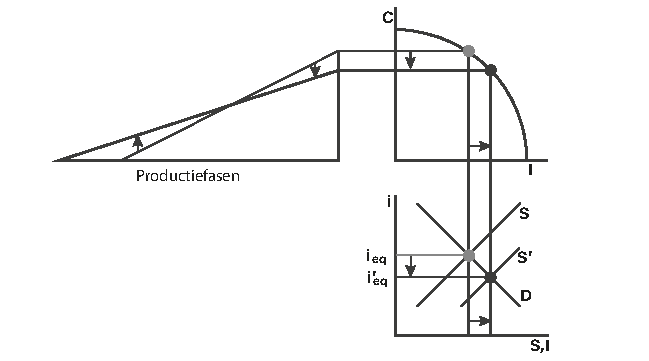
\includegraphics[width=\textwidth]{figures/fig32.pdf}
    \caption[Economische groei door investeringen en uitstel van consumptie\index{consumptie}]{Economische groei door investeringen en uitstel van consumptie\index{consumptie}}
    \label{fig32}
\end{figure}

Zuivere 100\% gedekte geldcertificaten veroorzaken geen toename in de geldhoeveelheid. Elk geldcertificaat dat als lening\index{lening} wordt uitgegeven, komt overeen met een vaste hoeveelheid van een marktgoed dat wordt aangehouden door de uitgever van het bewijs. Geld wordt als een echt marktgoed door de spaarders ter beschikking gesteld van de lener. Dat offer maakt economische middelen vrij die gebruikt kunnen worden in de vroege fasen van het productieproces\index{productieproces}, in plaats van voor consumptiegoederen\index{consumptiegoed}.

De dingen zien er heel anders uit wanneer fiduciaire middelen worden uitgegeven in plaats van geldcertificaten. Fiduciaire middelen worden uitgegeven zonder dat de bank\index{bank} geld in kas heeft. Niemand hoeft economische goederen op te offeren. Grafisch gezien stelt kredietexpansie via fiduciaire middelen leners in staat om pogingen te ondernemen om de productieketen te verlengen zonder de vereiste opoffering van consumptie\index{consumptie}. Ondernemers proberen met leningen een beweging boven de productiemogelijkhedencurve te maken met een omvang van investeringen en consumptie die de totale hoeveelheid beschikbare middelen overschrijdt. Op de kapitaalmarkt verschuift de aanbodcurve op een kunstmatige manier door de leenbare middelen te verhogen en daarmee de rentevoet te verlagen. De daling van de rente\index{rente} komt echter niet overeen met een toename van de spaartegoeden\index{spaartegoeden} waarmee de toegenomen investeringen zijn te financieren. Integendeel, lagere rentetarieven ontmoedigen het sparen juist.

De hoeveelheid geïnvesteerde middelen, I2 in het voorbeeld van Figuur 33, is veel groter dan de hoeveelheid gespaarde middelen, S2. De monetaire expansie\index{monetaire expansie} zorgt er niet alleen voor dat ondernemers denken dat ze meer middelen hebben dan ze in werkelijkheid bezitten, het zorgt er ook voor dat er minder middelen beschikbaar zijn door sparen te ontmoedigen en dus meer consumptie\index{consumptie} te stimuleren. Het verschil tussen I2 en S2 in deze grafiek is het kapitaal\index{kapitaal} dat ging naar de financiering van wat Mises zogenoemde \textbf{waninvesteringen} noemt -- investeringen die niet zouden zijn gedaan zonder verstoringen op de kapitaalmarkt, en waarvan de voltooiing niet mogelijk is zodra deze verstoringen aan het licht komen.\autocite{177} Het falen van de investering om de gewenste output te produceren leidt tot een krimp van de productiemogelijkhedencurve, aangezien de hoeveelheid beschikbare middelen afneemt. De productiedriehoek wordt korter en de productieketen krimpt.

\begin{figure}
\centering
    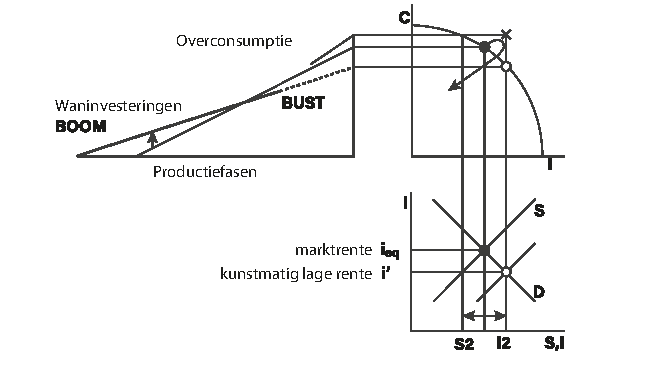
\includegraphics[width=\textwidth]{figures/fig33.pdf}
    \caption[Kredietexpansie met fiduciaire middelen en de conjunctuurcyclus\index{conjunctuurcyclus}]{Kredietexpansie met fiduciaire middelen en de conjunctuurcyclus\index{conjunctuurcyclus}}
    \label{fig33}
\end{figure}

De situatie is echter heel anders wanneer fiduciaire middelen worden uitgegeven in plaats van geldcertificaten, zoals geïllustreerd in Figuur 33. Fiduciaire middelen worden uitgegeven zonder dat de bank\index{bank} er de dekking voor bezit. Ze vereisen dus geen opoffering van economische goederen, door wie dan ook. Grafisch uit kredietexpansie door middel van fiduciaire middelen zich in het verlengen van de productieketen (de opwaartse pijl in de driehoek op Figuur 33) zonder de benodigde vermindering van de consumptie\index{consumptie} (de stippellijn in de driehoek en de witte stip in de PMC). Kredietnemende ondernemers proberen in feite om voorbij de productiemogelijkhedengrens te gaan met een hoeveelheid investeringen en consumptie\index{consumptie} die de totale hoeveelheid beschikbare middelen overschrijdt (het kruis in de PMC).

Op de kapitaalmarkt komen de opportuniteitskosten van kapitaal uit de opgeofferde consumptie en de opportuniteitskosten van consumptie zijn niet-gemaakte kapitaalinvesteringen. De rentevoet is de prijs die deze relatie regelt: naarmate mensen meer investeringen vragen, stijgt de rentevoet, waardoor meer spaarders worden gestimuleerd om meer van hun geld opzij te zetten om te sparen. Als de rente daalt, stimuleert dit producenten om meer te investeren in meer technologisch geavanceerde productiemethoden met een langere tijdsduur. Een lagere rente maakt dus langere productieketens met een hoge productiviteit mogelijk. Hierdoor kan de maatschappij evolueren van vissen met hengels naar vissen met grote door olie aangedreven boten.

Naarmate een economie zich ontwikkelt en steeds geavanceerder wordt, verandert het verband tussen fysiek kapitaal\index{kapitaal} en de markt voor uitleenbare middelen in werkelijkheid niet, maar het wordt wel ondoorzichtiger in de hoofden van mensen. Een moderne economie met een centrale bank\index{centrale bank} is gebaseerd op het negeren van deze fundamentele afweging en op de aanname dat banken investeringen kunnen financieren met nieuw gecreëerd geld zonder dat consumenten hoeven af te zien van consumptie\index{consumptie}. Het verband tussen het sparen en de uitleenbare middelen is dusdanig verbroken dat het niet eens meer in economische leerboeken wordt onderwezen. In een standaard leerboek wordt de aanbodcurve voor uitleenbaar geld afgebeeld als een rechte verticale lijn waarvan de grootte wordt bepaald door beleidsmakers. In het Keynesiaanse alternatieve universum bepalen centrale banken eenvoudigweg de geldhoeveelheid en de rentevoet en er wordt aangenomen dat de fysieke middelen vanzelf tevoorschijn zullen komen om de nominale monetaire fantasieën van de bank\index{bank} te realiseren.

Reële productiemiddelen kunnen natuurlijk niet in het leven worden geroepen door monetair beleid, dus het kunstmatig verlagen van de rente\index{rente} creëert onvermijdelijk een discrepantie tussen spaartegoeden\index{spaartegoeden} en uitleenbare middelen. Bij deze kunstmatig lage rente\index{rente} gaan bedrijven meer schulden aan om projecten te starten dan dat spaarders bereid zijn opzij te zetten voor de financiering ervan. Met andere woorden, de waarde van de uitgestelde consumptie\index{consumptie} is lager dan de waarde van het geleende kapitaal\index{kapitaal}. Zonder voldoende uitgestelde consumptie\index{consumptie} zullen er niet genoeg kapitaal\index{kapitaal}, land en arbeidskrachten worden overgeheveld van consumptiegoederen naar kapitaalgoederen van een hogere orde in de vroegste productiefasen. Er is immers geen spreekwoordelijke ``free lunch'' en als consumenten minder sparen, zal er minder kapitaal\index{kapitaal} beschikbaar zijn voor investeerders.

Dit tekort aan kapitaal\index{kapitaal} is niet direct zichtbaar omdat banken en de centrale bank\index{centrale bank} genoeg fiduciaire middelen kunnen uitgeven voor alle leners. Het creëren van nieuwe biljetten aan papiergeld of digitale tegoeden om het tekort aan spaargeld aan te vullen, vergroot niet op magische wijze de fysieke kapitaalvoorraad van de maatschappij. In plaats daarvan devalueert het de bestaande geldvoorraad en verstoort het de prijzen, waardoor producenten aan productieprocessen beginnen die meer kapitaal\index{kapitaal} vereisen dan er feitelijk beschikbaar is. Omdat steeds meer producenten zullen bieden op minder kapitaalgoederen\index{kapitaalgoederen} en middelen dan ze verwachten er te zijn, is het natuurlijke resultaat een stijging van de prijs\index{prijs} van de kapitaalgoederen\index{kapitaalgoederen} tijdens het productieproces\index{productieproces}. Dit is het moment waarop de manipulatie aan het licht komt, wat leidt tot de gelijktijdige ineenstorting van verschillende kapitaalinvesteringen die plotseling onrendabel worden tegen de nieuwe prijzen van de kapitaalgoederen\index{kapitaalgoederen}; de \emph{waninvesteringen}. De interventie van de centrale bank\index{centrale bank} in de kapitaalmarkt maakt het mogelijk dat er meer projecten worden ondernomen, maar vanwege de verstoring van de prijzen zullen investeerders verkeerde economische calculaties maken. Met andere woorden, interventie door de centrale bank\index{centrale bank} \emph{veroorzaakt} waninvesteringen. De interventie van de centrale bank\index{centrale bank} kan de hoeveelheid daadwerkelijk beschikbaar kapitaal\index{kapitaal} niet vergroten, dus de investeringsprojecten zullen uiteindelijk worden geconfronteerd met de harde economische realiteit, en moeten stop worden gezet. Het gevolg is dat het reële kapitaal\index{kapitaal} dat in de projecten is geïnvesteerd onnodig wordt verspild. Het stopzetten van deze projecten veroorzaakt tevens een stijging van de werkloosheid in de hele economie omdat een groot aantal mensen in veel sectoren hun onderneming zien mislukken of zich moeten aanpassen. Dit gelijktijdige economiebrede faillissement\index{faillissement} van bedrijven met overdreven investeringen wordt een \textbf{recessie\index{recessie}} genoemd.

Alleen met een goed inzicht in de werking van kapitaalstructuur en hoe rentemanipulatie de stimulans voor kapitaalaccumulatie vernietigt, kan men de oorzaken van recessies en de schommelingen van de conjunctuurcyclus\index{conjunctuurcyclus} begrijpen. De conjunctuurcyclus\index{conjunctuurcyclus} is het logische resultaat van de manipulatie van de rente\index{rente}, waardoor de kapitaalmarkt verstoort door de investeerders te laten denken dat ze meer kapitaal\index{kapitaal} kunnen verwerven dan beschikbaar is met het ondeugdelijke geld dat ze van de bank krijgen. In tegenstelling tot wat de Keynesiaanse animistische mythologie beweert, zijn conjunctuurcycli geen mystieke fenomenen die veroorzaakt worden door onvoorspelbare ``animal spirits''. Bij het maken van een herstelplan hebben centrale banken het het liefst dat de oorzaak van de cyclus buiten beschouwing wordt gelaten. Recessies zijn echter het onvermijdelijke logische gevolg van hun rentemanipulatie, net zoals tekorten het onvermijdelijke gevolg zijn van prijsplafonds. Keynesiaanse economie creëert de conjunctuurcyclus\index{conjunctuurcyclus} en verkoopt zichzelf vervolgens als de oplossing.

Een passende analogie om dit punt duidelijk te maken kan geleend (en verfraaid) worden uit het werk van Mises: stel je de kapitaalvoorraad van een samenleving voor als bouwstenen en de centrale bank\index{centrale bank} als een aannemer die ze gebruikt voor de bouw van huizen. Voor de bouw van elk huis zijn 10.000 bakstenen nodig en de projectontwikkelaar is op zoek naar een aannemer die 100 huizen kan bouwen, waar in totaal 1 miljoen bakstenen voor nodig zijn. Een Keynesiaanse aannemer die het contract graag wil binnenhalen, realiseert zich dat zijn kansen om het contract binnen te halen groter zijn als hij een offerte kan indienen waarin hij belooft 120 van die huizen te bouwen met maar 800.000 bakstenen. Dit is vergelijkbaar met rentemanipulatie: het vermindert het aanbod van kapitaal\index{kapitaal} terwijl de vraag ernaar toeneemt. In werkelijkheid zijn er voor 120 huizen 1,2 miljoen bakstenen nodig, maar er zijn er slechts 800.000 beschikbaar. De 800.000 bakstenen zijn voldoende om met de bouw van de 120 huizen te beginnen, maar niet om ze te voltooien. Als de bouw begint, is de ontwikkelaar erg blij dat hij 20\% meer huizen ziet voor 80\% van de kosten. De geweldige Keynesiaanse bouwkunde heeft ervoor gezorgd dat hij de 20\%, die hij nu bespaart, kan uitgeven aan een nieuwe zeilboot.

Helaas kan het bedrog niet blijven aanhouden, want uiteindelijk zal blijken dat de huizen niet kunnen worden afgebouwd en de bouw zal moeten worden stilgelegd. Niet alleen is de aannemer er niet in geslaagd om de 120 huizen op te leveren, maar hij zal zelfs helemaal geen huizen opleveren. In plaats daarvan heeft hij de ontwikkelaar achtergelaten met 120 onafgemaakte huizen, in feite nutteloze stapels bakstenen zonder dak. Het bedrog van de aannemer verminderde het kapitaal\index{kapitaal} dat door de ontwikkelaar werd uitgegeven en resulteerde in de bouw van minder huizen dan mogelijk zou zijn geweest met juiste prijssignalen. De ontwikkelaar zou 100 huizen hebben gehad als hij met een eerlijke aannemer in zee was gegaan. Door in zee te gaan met een Keynesiaanse aannemer die de cijfers manipuleert, blijft de ontwikkelaar zijn kapitaal\index{kapitaal} verspillen zolang het kapitaal\index{kapitaal} wordt toegewezen volgens een plan dat geen basis heeft in de realiteit. Als de projectontwikkelaar zich al in een vroeg stadium van de bouw van de 120 huizen bewust wordt van zijn fout, is het verspilde kapitaal\index{kapitaal} misschien heel beperkt en kan een nieuwe aannemer de overgebleven stenen gebruiken om 90 huizen te produceren. Als de ontwikkelaar onwetend blijft van de realiteit totdat het kapitaal\index{kapitaal} op is, zal hij eindigen met 120 onafgemaakte huizen die waardeloos zijn, omdat niemand zal betalen om in een huis zonder dak te wonen.

Wanneer de centrale bank\index{centrale bank} de rente\index{rente} tot onder de marktprijs manipuleert door banken meer geld te laten creëren door het verstrekken van leningen, verlagen ze tegelijkertijd de hoeveelheid spaargeld die beschikbaar is in de samenleving en verhogen ze de hoeveelheid die wordt gevraagd door leners. Dit terwijl ze ook het geleende kapitaal\index{kapitaal} sturen naar projecten die niet kunnen worden voltooid. Wanneer een overheid\index{overheid} het pad van het opblazen van de geldhoeveelheid is opgegaan, is er niet te ontkomen aan de negatieve gevolgen. Als de centrale bank\index{centrale bank} de monetaire expansie\index{monetaire expansie} stopt, stijgen de rentetarieven en volgt er een recessie\index{recessie} omdat veel van de gestarte projecten verlieslatend blijken te zijn en moeten worden opgegeven. Hierdoor komt de verkeerde allocatie van productiemiddelen en kapitaal\index{kapitaal} aan het licht. Als de centrale bank\index{centrale bank} haar inflatoire proces oneindig zou voortzetten, zou zij de omvang van de misallocaties in de economie alleen maar vergroten, waardoor nog meer kapitaal\index{kapitaal} wordt verspild en de onvermijdelijke recessie\index{recessie} nog pijnlijker wordt. Er is geen ontkomen aan het betalen van een flinke rekening voor de veronderstelde gratis lunch die Keynesiaanse gekken ons hebben opgedrongen.

Friedrich Hayek vergeleek kredietexpansie met het vangen van een tijger bij zijn staart. Als je de tijger eenmaal bij zijn staart hebt, begint hij te rennen en zijn er geen goede oplossingen meer.

\begin{blockquotebox}
We hebben nu een tijger bij de staart: hoelang kan deze inflatie\index{inflatie} nog doorgaan? Als de tijger wordt vrijgelaten zal hij ons opeten; maar als hij steeds sneller rent terwijl wij wanhopig blijven volhouden, zijn we nog steeds de pineut! Ik ben blij dat ik hier niet zal zijn om de uiteindelijke uitkomst te zien.\footnotemark
\end{blockquotebox}
\autocite{178}


\section{Centrale planning van de kapitaalmarkt}

Fiduciaire middelen zijn financiële producten die op natuurlijke wijze zouden kunnen ontstaan op een vrije markt, maar het is volstrekt onwaarschijnlijk dat ze lang zouden overleven. Ze zouden op de markt kunnen ontstaan door de unieke aard van geld als een goed waarvan het enige doel is om het te ruilen voor iets anders, waardoor een claim op geld schijnbaar net zo goed is als geld door het feit dat ze beiden kunnen worden geruild voor goederen. Fiduciaire middelen zouden echter niet lang overleven op een vrije markt, omdat ze de uitgever ervan blootstelt aan het risico\index{risico} van faillissement\index{faillissement} als een bepaald percentage van hun schuldeisers probeert om de fiduciaire middelen weer in te wisselen voor geld.

Onder de goudstandaard\index{goudstandaard} werden fiduciaire middelen veel gebruikt, maar ze leidden tot periodieke financiële crises waarbij grote bedragen werden weggevaagd of sterk ontwaard. Fiduciaire middelen konden overleven onder een goudstandaard\index{goudstandaard} omdat een aanzienlijk deel van de totale geldhoeveelheid te allen tijde op de bank\index{bank} zou blijven staan. Veel eigenaren gaven er namelijk de voorkeur aan om hun geld op de bank\index{bank} te houden, waar het gebruikt kon worden voor het afwikkelen van betalingen tegen veel lagere kosten dan door het verplaatsen van fysiek goud\index{goud}. Persoonlijk betalen met fysiek goud\index{goud} buiten iemands woonplaats was praktisch onbetaalbaar, en de vooruitgang van transport- en telecommunicatietechnologie betekende dat steeds meer transacties van een individu plaatsvonden over lange afstanden. Dit resulteerde in een steeds groter percentage van het goud\index{goud} dat op de bank\index{bank} moest blijven staan om de verkoopbaarheid\index{verkoopbaarheid} ervan over afstand te vergroten. Elke keer dat een houder van een bankbiljet ervoor koos om het te verzilveren voor fysiek goud\index{goud}, koos hij voor een grote afname van de verkoopbaarheid\index{verkoopbaarheid} van zijn geld over afstand. Dit gaf banken een foutmarge bij de uitgifte van fiduciaire middelen, omdat ze wisten dat niet al hun klanten op hetzelfde moment om uitbetaling zouden vragen.

Deze veiligheidsmarge werkt zichzelf: hoe veiliger de bank\index{bank} is, hoe meer fiduciaire middelen ze uitgeeft, hoe minder veilig ze wordt en hoe vatbaarder ze zal zijn voor een bankrun. Deze bankruns zullen periodiek plaatsvinden en desastreus zijn voor veel betrokkenen. Een vrije markt in geld en bankieren zal waarschijnlijk banken en klanten die zich bezighouden met de uitgifte van ongedekt krediet\index{krediet} blijven wegvagen totdat het verschijnsel helemaal verdwijnt. De marginale kosten voor een bank\index{bank} om fiduciaire middelen te produceren zijn bijna nul, en een vrije bancaire markt zal fiduciaire middelen blijven leveren, totdat hun prijs\index{prijs} gelijk is aan de productiekosten. Dit betekent in feite dat de fiduciaire middelen zullen worden gedevalueerd totdat ze geldcertificaten worden en een nominale waarde hebben die gelijk is aan de dekking die er is om ze in te wisselen.

In de negentiende-eeuwse Verenigde Staten\index{Verenigde Staten} voorkwamen monopolistische bankvergunningen op concurrentie op de vrije markt de sanering van fiduciaire middelen.ervoor zorgde dat de fiduciaire middelen verdwenen. Zolang de toegang tot het bankwezen beperkt was, was het voor de gevestigde bedrijven winstgevend om fiduciaire middelen te produceren, ook al veroorzaakten ze periodieke crises en economische ineenstortingen. Periodieke overheidsinterventies in het banksysteem en de oprichting van de eerste en tweede centrale banken van de VS zouden de banken helpen beschermen tegen de gevolgen van ongedekte kredietexpansie op de vrije markt. Een grote financiële crisis in 1907 richtte de aandacht van de leiders van de financiële sector op de noodzaak om een derde monopolistische centrale bank\index{centrale bank} op te richten die klaarstond om bankinstellingen te redden in tijden van financiële crises. In 1913 werd de \textit{U.S. Federal Reserve Act\index{Federal Reserve Act}} aangenomen en kreeg de nieuwe centrale bank\index{centrale bank} het inherent tegenstrijdige tweeledige mandaat om de waarde van de valuta te beschermen en tegelijkertijd banken te redden van financiële crises. In de afgelopen eeuw bestond de prijs voor het beschermen van ongedekte kredieten tegen een juiste beoordeling door de markt, uit het constant ontwaarden van de munt. Terwijl in de negentiende eeuw de uitgifte van fiduciaire middelen financiële crises en onrust veroorzaakte, bleef dit relatief binnen de perken en beperkt tot mensen die vrijwillig betrokken waren bij deze financiële instellingen. De eigenaars van goud\index{goud} hadden niets te vrezen, aangezien de marktprijs van hun geld grotendeels onaangetast bleef. In de twintigste eeuw werden financiële crises bijna altijd verzacht en opgelost door de devaluatie van het geld dat in handen was van mensen die niet eens betrokken waren bij de insolvabele instituten.

In plaats van een manier te bieden om investeringen en productiviteit te verhogen, is kredietexpansie ongedekt door reële besparingen in de negentiende eeuw een recept gebleken voor financiële crises en de oorzaak van de vernietiging van gezond geld\index{gezond geld} in de twintigste eeuw. Om de financiële instellingen te beschermen tegen de gevolgen van ongedekte leningen, werd een socialistische centrale planningsinstantie ingesteld voor voor de markt voor geld en kapitaal\index{kapitaal} aangesteld de belangrijkste markt en het integrale onderdeel van alle andere markten\index{markten}.

Hoewel de meeste mensen denken dat socialistische samenlevingen tot het verleden behoren en dat marktsystemen heersen over kapitalistische economieën, kan een kapitalistisch systeem in werkelijkheid niet functioneren zonder een vrije kapitaalmarkt. De prijs\index{prijs} van kapitaal\index{kapitaal} dient te ontstaan door de interactie van vraag en aanbod en de beslissingen van kapitalisten horen te worden gestuurd door accurate prijssignalen. Recessies en financiële crises kunnen het best worden begrepen als het falen van kapitaalmarkten wanneer centrale planning de monetaire vrijheid beperkt. De bemoeienis met de kapitaalmarkt door monopolistische centrale banken is de oorzaak van recessies en financiële crises. Toch schrijft de meerderheid van politici, journalisten en academici deze centraal geplande rampen steevast toe aan het kapitalisme\index{kapitalisme}.

De mislukking die optreedt bij centrale planning op de kapitaalmarkt wordt de conjunctuurcyclus\index{conjunctuurcyclus} genoemd, zoals uitgelegd in de Oostenrijkse conjunctuurtheorie. Het is dus geen wonder dat dit disfunctioneren wordt behandeld als een normaal onderdeel van markteconomieën, want in de hoofden van moderne economen is een centrale bank\index{centrale bank} die de rente\index{rente} controleert immers een normaal onderdeel van een moderne markteconomie. Een centrale bank\index{centrale bank} is echter net zo\textquotesingle n normaal onderdeel van een kapitaalmarkt als een monopolistisch aardappelagentschap een normaal onderdeel is van aardappelmarkten.

Schrijvers van de Oostenrijkse School\index{Oostenrijkse School} hebben de monetaire geschiedenis nauwgezet gedocumenteerd in een aantal boeken die sterk zijn aan te raden, waarin de Oostenrijkse theorie wordt gebruikt om ons inzicht in de geschiedenis te verhelderen. Vaak wordt deze vertroebeld door de behoefte van overheidshistorici om de acties van de staat en zijn monetaire rampen te verbloemen. Vooral Hayek\textquotesingle s \emph{Monetary Nationalism and International Stability} , Rothbard\textquotesingle s \emph{America\textquotesingle s Great Depression} en \emph{A History of Money and Banking in the United States}, en Ferdinand Lips\textquotesingle{} \emph{Gold Wars} zijn goede voorbeelden. Deze geschiedenis wijst op een aantal ongelukkige, rampzalige en terugkerende patronen in de ontwikkeling van het moderne bankwezen en het overheidsbeleid.

Op de korte termijn hopen regeringen en centrale bankiers hun doelen te bereiken door geld te ontwaarden om kredietschepping en uitgaven voor belangrijke doelen te financieren. Regeringen denken misschien dat ze de economie stimuleren of mensen beschermen tegen de gevolgen van vrije markten\index{markten}, maar door het geld te devalueren om deze doelen te bereiken, creëren ze waninvesteringen en zaaien ze de kiem voor grote schade op de lange termijn. Pogingen om de economie te redden van de onvermijdelijke crises die daar het gevolg van zijn, resulteren in verdere kredietschepping en reddingsoperaties die onverantwoord gedrag aanmoedigen, de verkwisters belonen en de voorzichtige mensen straffen. Op die manier zorgen centrale banken er eigenlijk voor dat de conjunctuurcyclus\index{conjunctuurcyclus} een vast onderdeel wordt van een economie en dat hun macht over de markt groeit. Na verloop van tijd is het resultaat de vernietiging van kapitaal\index{kapitaal}, geld, het vermogen om te sparen en van de arbeidsdeling\index{arbeidsdeling} zelf. Geld in handen geven van een overheidsmonopolie is verre van een wondermiddel; het vernietigt de fundamenten waarop de menselijke samenleving en de moderne kapitalistische beschaving\index{beschaving} zijn gebouwd.



\part{BESCHAVING}
\hypertarget{geweld}{%
\chapter{Geweld}\label{geweld}}

\vspace{-1em}
\lettrine{A}lle menselijke economische handelingen die dit boek tot nu toe heeft behandeld, zijn op vrijwillige basis. Deel II besprak vrijwillige economische handelingen die individuen uit eigen initiatief ondernemen om de kwaliteit en kwantiteit van hun tijd te vergroten. Deel III heeft het marktsysteem uitgelegd dat voortkomt uit de sociale interacties die individuen vrijwillig aangaan om eveneens de kwaliteit en kwantiteit van hun tijd te verbeteren. In elk onderdeel hebben de betrokken individuen uit vrije wil gehandeld, zowel individueel als in samenwerking met anderen. Dat is echter niet de enige manier waarop mensen met elkaar om kunnen gaan. Ze kunnen ook de kwaliteit en de kwantiteit van hun tijd op aarde verbeteren door geweld te gebruiken of anderen met geweld te bedreigen. Ze kunnen het lichaam en het eigendom van anderen aanvallen met als doel hun eigendom af te pakken of mogelijk zelfs de ander tot slaaf te maken. Geweld, en de dreiging van geweld, leiden tot \textbf{dwang}: de oplegging van iemands wil aan een ander.

\hypertarget{non-agressieprincipe}{%
\section{Non-agressieprincipe}\label{non-agressieprincipe}}

Economie beschouwt geweld en dwang niet als irrelevant, maar bestudeert ze als vormen van menselijk handelen, waarvan de gevolgen kunnen worden onderzocht en vergeleken met vrijwillige overeenkomsten. Het fundamentele verschil tussen vrijwillige en onvrijwillige interactie is dat alle deelnemers in een vrijwillige interactie verwachten ervan te profiteren, terwijl iemand negatieve gevolgen kan verwachten in een onvrijwillige interactie (anders zouden ze niet gedwongen hoeven te worden). Hoewel vrijwillige ruilhandel niet altijd het beoogde resultaat oplevert voor alle betrokken partijen, garandeert het uitoefenen van dwang dat één partij zeker ongewenste gevolgen zal ondervinden. Mensen die geen voordeel blijken te halen uit hun gezamenlijke overeenkomst, kunnen hun verwachtingen herzien en de overeenkomst opzeggen of hun strategie aanpassen in de hoop op een betere uitkomst. Slachtoffers van dwang hebben deze mogelijkheid niet, omdat hun wensen niet worden gerespecteerd door de toepassing van geweld of de dreiging ervan. Interacties onder dwang kunnen voortduren zolang de dader de negatieve gevolgen van de agressie niet ondervindt.

De negatieve gevolgen van dwang en agressie kunnen vergeleken worden met natuurrampen of aanvallen door dieren. Net zoals voor deze situaties, hebben mensen al lang naar manieren gezocht om zichzelf tegen dwang en geweld te beschermen. Vergelijkbaar met hoe mensen werken, kapitaal\index{kapitaal} opbouwen, handelen en innoveren, leren ze zich ook te verdedigen en ontwikkelen ze steeds complexere en effectievere manieren om zichzelf en hun eigendom te beschermen tegen de agressie van anderen. Hoofdstuk 17 gaat in op verschillende verdedigingsstrategieën tegen agressie. De rest van dit hoofdstuk onderzoekt een specifieke vorm van agressie: overheidsagressie.

In ethische en economische zin is er een zeer belangrijk onderscheid tussen geweld, en het initiëren van geweld. Het initiëren van geweld schendt het eigendomsrecht op het lichaam of eigendom van het slachtoffer, wat leidt tot vijandigheid en mogelijk zelfs vergelding door het slachtoffer. Ook kan het leiden tot het uitsluiten van de dader door anderen binnen de samenleving. Dit maakt vreedzame samenwerking moeilijker en voorkomt de groei van de marktomvang en de arbeidsdeling\index{arbeidsdeling}. De mate waarin groepen mensen, klein of groot, het initiëren van geweld verwerpen, geeft aan hoe ver de marktorde is ontwikkeld en tot welke mate de samenleving kan profiteren van de arbeidsdeling\index{arbeidsdeling}. Hoe meer het initiëren van geweld door sommige leden van een groep wordt geaccepteerd, des te meer conflict er zal ontstaan en de samenwerking, die noodzakelijk is voor de marktorde, zal worden ondermijnd. Het legitimeren van agressie voor één individu of groep, maar niet voor anderen, is geen morele standaard die consequent op de samenleving toegepast kan worden.

Geweld kan echter wel ethisch acceptabel worden beschouwd wanneer het wordt ingezet ter zelfverdediging of om agressors af te weren of te bestraffen. Legitieme zelfverdediging kan daarom ook goed samen gaan met een brede marktorde. Leden van een marktorde kunnen allemaal samenwerken als ze allemaal akkoord gaan met één universele regel die op hen allen van toepassing is: de onwettigheid van het initiëren van agressie en de legitimiteit van zelfverdediging. Deze asymmetrie tussen geweld en het initiëren van geweld, en de implicaties voor de marktorde, vormen de basis voor het \textbf{non-agressieprincipe}, dat Rothbard als volgt omschrijft:

\begin{blockquotebox}
Niemand mag dreigingen uiten of geweld plegen (`agressie') tegen een ander persoon of diens eigendom. Geweld mag alleen ingezet worden tegen de persoon die zelf dit geweld pleegt; met andere woorden, enkel en alleen in verdediging tegen de agressieve daad van een ander. Kortom, geweld mag niet ingezet worden tegen een niet-agressor.\footnotemark
\end{blockquotebox}
\footautocite{179}

Het non-agressieprincipe, geformuleerd en gepopulariseerd door Rothbard en andere Oostenrijkse economen, vindt zijn historische wortels in diverse beschavingen en tijdperken doorheen de geschiedenis, zoals Edward Fuller heeft vastgelegd in zijn paper.

\begin{blockquotebox}
Een grote en diverse groep van de meest vooraanstaande denkers uit de geschiedenis hebben ideeën geuit die zeer vergelijkbaar zijn met het non-agressieprincipe. De beginselen van het principe waren bekend bij de oude Egyptenaren rond 2000 v.Chr., bij de oude Hindoes rond 1500 v.Chr., en bij de oude Hebreeërs rond 1000 v.Chr. Rond 500 v.Chr. formuleerden de oude Chinese en Griekse filosofen de onderliggende logica van het principe. Cicero kwam dicht bij het formuleren van het principe in zijn moderne vorm. Thomas van Aquino kwam uit op iets wat opvallend gelijk was aan het non-agressieprincipe na de vroege middeleeuwen, en de scholastische filosofen droegen het idee over naar de vroege moderne tijd. In de zeventiende eeuw bereikte het non-agressieprincipe de top van de Westerse filosofie.\footnotemark
\end{blockquotebox}
\footautocite{180}

Veel economische boeken, waaronder dit boek, gebruiken het verhaal van Robinson Crusoë op een onbewoond eiland als middel om de werkelijkheid van economische productie\index{productie} en de voordelen van vreedzame samenwerking te verduidelijken. Het verhaal vindt zijn oorsprong in een fictieve roman, \emph{Hayy Ibn Yaqdhan}, geschreven door de Arabische filosoof Ibn Tufayl. Dit uitgangspunt werd door hem gebruikt om te illustreren hoe een mens, zelfs wanneer geboren in totale afzondering van de mensheid, een begrip van moraliteit kan ontwikkelen.

\hypertarget{overheidsdwang}{%
\section{Overheidsdwang}\label{overheidsdwang}}

De meeste gangbare stromingen binnen de economie en politiek presenteren de overheid\index{overheid} als de oplossing voor het probleem van agressie binnen de samenleving. Gezien het feit dat geweld en agressie altijd aanwezig zullen zijn, is een instelling met een monopolie op geweld volgens hen de enige manier om op ieder vlak een beschaafde en vreedzame sociale orde te bewerkstelligen. Als alle inwoners de legitimiteit van de monopolist accepteren (vrijwillig of anderszins), worden gewelddadige handelingen, die gepleegd worden door een andere instelling, als illegaal en strafbaar beschouwd door de monopolist.

In de negentiende en twintigste eeuw draaiden de politieke en intellectuele debatten voornamelijk om de juiste rol van de staat in de samenleving, en niet zozeer om de legitimiteit of noodzaak ervan. Mises en de klassieke liberalen zagen het beschermen van haar burgers en hun eigendommen en het garanderen van hun veiligheid tegen agressie en diefstal als de juiste rol van de overheid\index{overheid}.

\begin{blockquotebox}
    De overheid\index{overheid} dient alle taken te vervullen waarvoor ze nodig is en waarvoor ze is opgericht. De overheid\index{overheid} moet het volk beschermen tegen het gewelddadige en frauduleuze gedrag van misdadigers, en ze moet het land verdedigen tegen buitenlandse vijanden. Dit zijn de functies van de overheid\index{overheid} binnen een vrij systeem, binnen het systeem van de vrijemarkteconomie.
    \par\vspace{1em}\noindent
    Onder socialisme is de overheid\index{overheid} van nature totalitair en er is niets buiten haar invloedssfeer en jurisdictie. In de markteconomie is de belangrijkste taak van de overheid\index{overheid} echter om het soepel functioneren van de markteconomie te beschermen tegen fraude of geweld van zowel binnen het land als van buitenaf.\footnotemark
\end{blockquotebox}
\footautocite{181}

Door het recht op eigendom te waarborgen, zal de overheid\index{overheid} individuen in staat stellen om te plannen voor de toekomst, hun tijdsvoorkeur\index{tijdsvoorkeur} te verlagen, kapitaal\index{kapitaal} te accumuleren, de productiviteit te verhogen en hun leven te verbeteren. Klassieke liberalen waarschuwen echter dat als een overheid\index{overheid} haar mandaat niet beperkt tot het beschermen van eigendom en de handhaving van wet en orde, dat zij dan meer kwaad dan goed zal doen. Haar interventies in de markteconomie zullen niet de beoogde doelen bereiken, voornamelijk vanwege het probleem van economische calculatie zonder duidelijk gedefinieerde eigendomsrechten (dit wordt besproken in Hoofdstuk 12). Als de overheid\index{overheid} eigenaar is van de kapitaalgoederen\index{kapitaalgoederen}, dan is er geen markt voor deze goederen en dus geen mogelijkheid om economische calculatie te verrichten met betrekking tot de alternatieve gebruiksmogelijkheden van deze middelen of om te bepalen hoe ze kunnen worden gealloceerd. Wanneer overheidsbureaucraten middels dwang beslissingen nemen over andermans eigendom, doen ze dat blindelings, zonder kennis van de belangrijkste factor die het inzetten van middelen bepaalt, namelijk de subjectieve voorkeuren van de betrokken individuen. Economische calculatie zonder eigendomsrechten resulteert in het verkeerd inzetten van middelen, verspilling en kapitaalvernietiging.

Een opmerkelijk aantal werken is gepubliceerd over de tekortkomingen van overheidsinterventie in de economie, zowel door economen uit de Oostenrijkse school als door mainstream etatistische economen.\autocite{182} Het vervolg van dit hoofdstuk zal de mislukkingen behandelen van enkele van de meest gangbare en breed ondersteunde vormen van overheidsinterventie in de individuele besluitvorming binnen een kapitalistische economie. Door gebruik te maken van de lens van menselijk handelen\index{menselijk handelen} en door inzicht te verkrijgen in de kenmerken van de opkomende marktorde, kunnen we de economische gevolgen onderzoeken van specifieke vormen van overheidsdwang.

Prijscontroles vormen misschien wel de populairste methode van overheidsinterventie in de economie en lijken een verleidelijke oplossing voor echte problemen, maar ze hebben enorme gevolgen, zowel positief voor sommigen als negatief voor velen. De logica achter prijscontroles lijkt eenvoudig en aantrekkelijk: indien de prijs\index{prijs} van een goed te hoog is, kan de overheid\index{overheid} een maximumprijs instellen, waardoor het verkopen tegen een hogere prijs\index{prijs} illegaal wordt en verkopers worden gedwongen hun waren tegen een lagere prijs\index{prijs} aan te bieden. Op deze manier kunnen mensen die de hogere prijs\index{prijs} niet kunnen betalen, toch de goederen tegen een lagere prijs aanschaffen. In \emph{Forty Centuries of Wage and Price Controls: How Not to Fight Inflation}, geven Robert Schuettinger en Eamonn Butler een uitgebreid historisch overzicht van de mislukkingen van prijscontroles door vierduizend jaar en over talloze plaatsen heen. Een alarmerend aantal regeringen heeft door de geschiedenis heen geprobeerd om met deze methode de prijzen van allerlei goederen, van voedsel tot huur, te reguleren. Er is geen enkel bewijs dat prijscontroles succesvol zijn geweest in het verlagen van prijzen; ze resulteren slechts in tekorten, zwarte markten\index{markten} en het ontstaan van uiterst inefficiënte manieren om schaarse voorraden te rantsoeneren.

Als prijscontroles dan toch enig effect hebben, is het dat ze mensen verhinderen te handelen tegen een prijs\index{prijs} waarvoor ze bereid waren te handelen. Wanneer handel wordt verboden tegen de marktprijs, zal de producent logischerwijs minder goed in staat zijn om het product op een winstgevende manier te produceren. Zonder de inkomsten van de originele hogere prijs\index{prijs} zal de producent niet genoeg van de benodigde middelen kunnen kopen om het product te produceren. Overheidsdwang kan de producent wel verbieden om boven de maximumprijs te verkopen, maar het kan hem niet dwingen te verkopen tegen die maximumprijs omdat hij er simpelweg voor kan kiezen om te stoppen met produceren. Het effect van deze interventie zal onvermijdelijk de levering van het product op de markt verminderen.

Een ander waarschijnlijk gevolg is de opkomst van een zwarte markt, waar goederen illegaal worden verkocht tegen hogere prijzen. De zwarte markt omzeilt de schade die overheidsinterventie veroorzaakt en geeft de mensen de mogelijkheid om de producten die ze nodig hebben alsnog te kopen. Maar het leidt wel tot verspilling voor de betrokken partijen. In plaats van schaarse middelen te wijden aan het produceren van het gewenste product, moeten producenten extra kosten maken die horen bij de illegale verkoop en distributie van hun product. Bovendien riskeren ze vervolging, inbeslagname en gevangenisstraffen. Hierdoor zullen speciale organisaties ontstaan die de verkoop van het product regelen en een groot deel van de winst ontvangen, in plaats van dat het wordt besteed aan investeringen in kapitaalgoederen\index{kapitaalgoederen} voor de productie\index{productie} van meer van het schaarse product. Het invoeren van prijscontroles verandert niet op magische wijze de economische waardering van goederen en hun productiekosten. Het maakt het alleen illegaal om de goederen te verhandelen tegen de prijzen die de producenten vragen. Dat betekent in feite een subsidie voor de criminele sector. Voor mensen die gewend zijn om buiten de wet te opereren, is dit lucratief. Middelen die naar de producenten hadden kunnen gaan om meer investeringen mogelijk te maken, gaan naar de misdaad\index{misdaad}.

Zodra tekorten na de invoering van prijscontroles onvermijdelijk optreden, zal de vraag naar het goed het aanbod beginnen te overtreffen. Dit zal nieuwe mechanismen om het aanbod onder consumenten te verdelen noodzakelijk maken. Een typisch voorbeeld is in de wachtrij staan. Hierbij besteden consumenten hun kostbare tijd aan het wachten in de rij totdat het product beschikbaar komt. Omdat tijd schaars is, zorgt in de rij staan er alleen maar voor dat de kosten van het goed worden overgebracht van geld naar tijd. Consumenten betalen nu voor het product met tijd die ze hebben verspild, iets wat niet door de producent kan worden gebruikt om meer van het goed te maken.

Voor sommige andere economische goederen zal gewelddadige overheidsinterventie proberen een hogere prijs\index{prijs} op te leggen op de markt dan de prijs\index{prijs} die voortkomt uit vrijwillige handel. Dit wordt voornamelijk toegepast bij lonen, waar overheden sinds lang hogere lonen voor werknemers proberen op te leggen. Het fiasco van het minimumloon wordt in detail uitgelegd in Hoofdstukken 1 en 4.

Het probleem van prijzen heeft bijna altijd zijn wortels in inflatie\index{inflatie}, wat het resultaat is van dwingende overheidsbemoeienis in de geldmarkt. Zoals besproken in Hoofdstuk 10, verschijnt geld op de markt als het goed met de beste verkoopbaarheid\index{verkoopbaarheid} door tijd -- het goed dat het best zijn waarde in de loop van de tijd behoudt. Aangezien men kan verwachten dat de beschikbare hoeveelheid het minst snel zal stijgen van alle andere marktgoederen, neigt de waarde van geld in waarde te stijgen, aangezien relatief meer van alle andere goederen dan van geld worden geproduceerd. In zo\textquotesingle n wereld zouden de prijzen van alle goederen de neiging hebben te dalen ten opzichte van het geld, terwijl de werkelijke lonen stijgen, zelfs als ze constant blijven of dalen in nominale termen. Als er echter dwingende interventie in de geldmarkt is, dan daalt de waarde van geld in de loop van de tijd, waardoor verkopers hun prijzen verhogen en de lonen van werknemers worden gedevalueerd. Het verhaal van inflatie\index{inflatie} is een al lang bestaand fenomeen, al werden er verschillende mechanismen toegepast: van Romeinse keizers die het goud\index{goud}- of zilvergehalte van hun munten\index{munten} verminderden en ze vervingen door koper en andere basismetalen, tot moderne overheden die grote hoeveelheden papiergeld drukken om rentetarieven te manipuleren, zodat er meer krediet\index{krediet} kan worden gecreëerd dan dat er spaarmiddelen\index{spaarmiddelen} in de samenleving zijn.\autocite{183} Inflatie ontneemt de welvaart van spaarders, devalueert hun geld en verhoogt de prijzen van de goederen die ze kopen, terwijl de overheid\index{overheid} met weinig beperkingen kan uitgeven.

De gangbare economische stromingen zullen mogelijk de problemen van monetaire inflatie\index{inflatie} voor geldbezitters en de economie in het algemeen erkennen, maar ze zien overheidsuitgaven als een goede zaak die deze problemen kan verlichten en helpen om maatschappelijke doelen te bereiken. Ze houden echter geen rekening met de werkelijke kosten. Begrip van opportuniteitskosten, de subjectieve aard van economie en de problemen van economische calculatie leiden tot de tegenovergestelde conclusie. Elke uitgave die door de overheid\index{overheid} wordt gedaan, moet worden gefinancierd met geld dat wordt ontnomen van productieve leden van de markteconomie, ten koste van hun eigen uitgaven. Mensen richten hun uitgaven om het best te voldoen aan hun behoeften. Het dwingend belasten van het inkomen van deze mensen om het geld vervolgens aan andere doeleinden te besteden, kan hun welzijn niet verhogen, omdat ze ervoor hadden gekozen dat geld zelf aan iets anders uit te geven. Geen enkele overheidsuitgave kan als vrijwillig worden beschouwd zolang inflatie\index{inflatie} en belasting niet vrijwillig zijn. Daarom kunnen overheidsuitgaven het best worden beschouwd als consumptieve uitgaven voor de mensen in overheidsinstellingen; het zijn geen investeringen.

Een andere veelvoorkomende vorm van overheidsinterventie is het verstrekken van subsidies aan individuen of het aanschaffen van specifieke goederen voor hen. Een simplistische kijk hierop veronderstelt dat overheidsuitgaven kosteloos zijn en dat overheden subsidies kunnen gebruiken om het welzijn van burgers te verbeteren. Echter, economische analyse laat zien dat dit niet het geval is. Overheidssubsidies verstoren de markt en sturen de beslissingen van mensen in een andere richting dan waar hun eigen beweegredenen en economische berekening hen normaal gesproken zouden leiden. Subsidies resulteren vaak in overproductie en overconsumptie van goederen, wat niet zou gebeuren als mensen vrijelijk zouden kunnen kiezen. Wanneer subsidies worden verstrekt op basis van iemands economische situatie, ontstaat er een sterkere prikkel voor mensen om die situatie te behouden om in aanmerking te komen voor de subsidies. Sociale bijstand kan bijvoorbeeld mensen met een laag inkomen aanmoedigen om op dat lage niveau te blijven. Subsidies voor werklozen kunnen leiden tot een grotere neiging tot werkloosheid. Bovendien, omdat subsidies gefinancierd worden ten koste van werkenden, kunnen ze de motivatie om te werken ondermijnen.

Overheidsvoorzieningen worden vaak gezien als een oplossing voor het probleem van ontoereikendheid of onbetaalbaarheid van goederen of diensten die ze biedt. Terwijl private bedrijven zich richten op winst, wordt door sommigen betoogd dat de overheid beter werk kan leveren door zich te concentreren op inclusie. Deze argumentatie wordt gebruikt ter ondersteuning van de overheidsvoorziening van goederen en diensten zoals onderwijs, water en gezondheidszorg. Echter, dit negeert de basisprincipes van kapitalistische economische productie. Winsten zijn niet alleen een middel voor hebzuchtige individuen om rijk te worden; ze vormen de coördinatie van de gehele structuur van marktproductie en stellen producenten in staat om de kosten en baten van verschillende opties te berekenen, terwijl ze streven naar het dienen van anderen en het behalen van optimale winsten voor henzelf. Het wegnemen van de winstmotivatie uit economische productie leidt niet tot onbaatzuchtige, overvloedige en betaalbare productie; het resulteert juist in een gebrek aan economische berekening, wat leidt tot aanzienlijke verspilling. Producten kunnen ongewenst zijn, wat leidt tot een verspilling van middelen, of als ze wel gewild zijn, kan het ontbreken van een vrije marktprijs leiden tot overmatige consumptie en problemen met beschikbaarheid voor gebruikers. \textquotesingle Gratis\textquotesingle{} door de overheid\index{overheid} aangeboden wegen eindigen bijvoorbeeld vaak vol met verkeer, wat grote vertragingen veroorzaakt voor reizigers die waarschijnlijk duurder zijn dan wat ze zouden betalen voor de aanleg van privéwegen. Door de overheid\index{overheid} aangeboden gezondheidszorg, in plaatsen als Canada, is berucht om het feit dat patiënten zeer lang moeten wachten voordat ze door een dokter kunnen worden ontvangen. Het is opmerkelijk dat in Canada, waar ze een vrije markt hebben in gezondheidszorg voor dieren, een ziek Canadees huisdier sneller een dokter ziet dan zijn eigenaar zelf.\autocite{184}

Overheidsuitgaven zijn schadelijk voor de economie, niet alleen omdat ze de berekening van winst en verlies van individuen verstoren, maar ook omdat ze gefinancierd moeten worden door belastingen, zowel direct als indirect via inflatie. Het belasten van producenten om overheidsuitgaven te financieren bestraft economische productie\index{productie}, wat de motivatie om eraan deel te nemen vermindert. Bovendien leidt de waardedaling van spaartegoeden\index{spaartegoeden} tot een afname van de stimulans om te sparen, terwijl belastingen op kapitaalwinsten de motivatie om te investeren verminderen. Door een persoon minder in staat te stellen om voor zijn of haar toekomst te zorgen, werken overheden de drijvende kracht achter de menselijke beschaving\index{beschaving} tegen, namelijk het verlagen van de tijdsvoorkeur\index{tijdsvoorkeur}.

Of het nu gaat om prijscontroles, landbouwsubsidies of belastingen, elke vorm van overheidsinterventie leidt tot gedwongen veranderingen in menselijk gedrag die onder vrije omstandigheden anders zouden zijn. Als mensen vrij gelaten zouden worden, zouden zij hun tijd en rijkdom besteden aan doelen die zij het meest waardevol achten, of dat nu productief is voor henzelf of voor anderen. Aangezien economische waarde zelf subjectief is, impliceert het wijzigen van iemands handelingen een afwijking van de door hem gekozen koers, die subjectief gezien minder zijn voorkeur geniet.

Gelukkig hebben de meeste mainstream economen, met name sinds het einde van de Sovjet-Unie, enig begrip getoond van de problemen met overheidsinterventie in het economische systeem en de verstorende gevolgen ervan. Zelfs het Samuelsoniaanse leerboek bevat nu een discussie over de problemen van overheidsinterventie in markten. Echter blijft de rechtvaardiging voor interventie onverminderd voortbestaan -- nu wordt het gepresenteerd alsof overheden 'marktfalen' oplossen, een term die mainstream economen gebruiken om een resultaat van vrije menselijke interactie aan te duiden waar ze het niet mee eens zijn.

\hypertarget{rechtvaardigingen-voor-overheidsgeweld}{%
\section{Rechtvaardigingen voor overheidsgeweld}\label{rechtvaardigingen-voor-overheidsgeweld}}

De moderne rechtvaardigingen voor overheidsingrijpen worden gewoonlijk gepresenteerd in de vorm van marktfalen: als mensen vrij gelaten worden om keuzes te maken, zullen ze inferieure en suboptimale resultaten opleveren. De initiële fout van deze benadering is dat de markt wordt gepresenteerd als een entiteit die niet in staat is om het gewenste resultaat te leveren. In werkelijkheid is de markt een overkoepelende term die mensen gebruiken om te verwijzen naar de handelingen van individuen die hun vrije wil uitoefenen om de tevredenheid in hun eigen leven te maximaliseren. De term `marktfalen' stelt een alwetende centrale planner voor die in staat is om te beslissen wat het optimale resultaat zou zijn van de vrije interacties van individuen, en vervolgens de acties van deze vrije individuen veroordeelt als inferieur en noodzakelijkerwijs te veranderen. Hoewel dit als voordelig voor het maatschappelijk welzijn wordt gepresenteerd, houdt deze benadering methodologisch gezien simpelweg in dat de wil van een centrale planner voorrang krijgt op de wensen van alle vrij handelende individuen.

De rijkelijk beloonde maar onleesbare artikelen die mainstream economen de afgelopen decennia aan de lopende band hebben gepubliceerd, bevatten een overdaad aan overheidspropaganda die zich voordoet als economische analyse. Hun benadering volgt een voorspelbaar script: een econoom verricht een grote hoeveelheid theoretisch, wiskundig of experimenteel werk om vervolgens te concluderen dat individuen die vrij handelen iets produceren dat suboptimaal is voor de samenleving als geheel, wat zij dan `marktfalen' noemen. Ze negeren gemakshalve de ethische vraag wat een academicus, die afhankelijk is van overheidssubsidies om te overleven, het recht geeft om te oordelen over de handelingen van anderen, en welk doel zij eigenlijk zouden moeten nastreven. De collectivistische benadering van economie gaat ervan uit dat waarde objectief is en dat een onpartijdige centrale planner precies kan weten hoeveel dat is. Het ontneemt individuen ook het recht om hun eigen beslissingen te nemen met betrekking tot hun eigendom, kapitaal en consumptie. Door economie voor te stellen als een objectieve wiskundige functie, terwijl economische waarde geen meeteenheid heeft, kunnen door de overheid gefinancierde economen alle benodigde cijfers tevoorschijn toveren om elke vorm van agressie tegen privaat eigendom te rechtvaardigen.

De oorsprong van deze analyse van het marktfalen komt voort uit het standaardmodel van de neoklassieke economie, wat probeerde om het marktproces wiskundig te modelleren. In plaats van de Oostenrijkse methode van individuele handelingen te volgen als basis voor het begrijpen van economie, probeerden moderne economen, in een gewaagde vertoning van cultwetenschap, de natuurkunde te kopiëren. Sinds de overname van de academische wereld door de overheid\index{overheid} in de jaren \textquotesingle30, probeert het merendeel van de economie voornamelijk natuurkundige concepten toe te passen op de ideeën van John Maynard Keynes\index{John Maynard Keynes} om zo rechtvaardigingen voor overheids- en centrale bankbeleid te verkrijgen. Wiskundige economen probeerden een wiskundig model uit de natuurkunde op de economische realiteit te leggen, maar wanneer ze werden geconfronteerd met een van de talloze onoverkomelijke obstakels tot het wiskundig modelleren van menselijke handelingen, werd de economische realiteit vereenvoudigd zodat het toepassen van de wiskundige modellen mogelijk werd. Enkele van de meest opmerkelijke aannames die voor de economie zijn bedacht, zijn 1) dat alle actoren in een marktsysteem volledige kennis moeten hebben; 2) dat ze op een rationele manier eigenbelang nastreven; en 3) dat er een toestand van perfecte concurrentie bestaat, met een oneindig aantal kopers en verkopers voor elke markt. Deze aannames houden uiteraard geen stand in de echte wereld, maar mainstream economen zien de onnauwkeurigheid van de aannames als bewijs van marktfalen in plaats van simpelweg te beseffen dat dergelijke wiskundige modellen nutteloos zijn!

Nadat het `marktfalen' is vastgesteld, stellen economen, zonder enig bewijs of analyse, dat overheidsinterventie deze geobserveerde inefficiëntie van de markt kan corrigeren. Ze publiceren deze onzin vervolgens in hoog aangeschreven tijdschriften, krijgen banen als docent aan universiteiten en ontvangen onderscheidingen en prijzen voor het bedenken van de rechtvaardigingen voor overheidsdwang en --- agressie tegen privaat eigendom. In de academische fiatwereld zijn er geen kosten verbonden aan het maken van fouten en zijn er zelfs beloningen voor het maken van fouten die de macht van de overheid vergroten.\autocite{185} De hele fiateconomie kan worden gezien als een uitgebreide oplichtingspraktijk, waarbij stromannen worden geplaatst en neergehaald en waarbij de ruimte die ze innamen wordt overgenomen alsof die van niemand was.

\subsection{Informatieasymmetrie}

Tot de meer modieuze argumenten voor economische interventie van de afgelopen decennia behoort de drogreden van `informatieasymmetrie'. Volgens de Keynesiaanse school vol onleesbaar onderzoek, beschikken individuen die deelnemen aan een transactie niet over volledige kennis van alles wat met de transactie te maken heeft, wat vaak leidt tot slechte resultaten. Dit is een volledig triviaal gegeven: het is onmogelijk voor een persoon om alles te weten wat de ander weet. Deze gedachte wordt echter gepresenteerd als bewijs om dwingende overheidsinterventie bij het maken van transacties mogelijk te maken. Toch vinden er elke dag wereldwijd miljarden markttransacties plaats, en de overgrote meerderheid daarvan is tot tevredenheid van beide partijen. Men hoeft niet alles te weten om te begrijpen wat een gunstige ruil\index{ruil} inhoudt -- men hoeft alleen maar te weten wat hun eigen voorkeur is voor de verhandelde goederen. Natuurlijk wordt in deze argumentatie ook geen rekening gehouden met het vraagstuk van hoe de dwingende regelgevende autoriteit toegang kan krijgen tot informatie die niet voor beide partijen beschikbaar is, en hoe zij die informatie kan gebruiken om met het dreigement van geweld een betere oplossing voor beide partijen af te dwingen. Hoe kan een regulerende instantie, die verantwoordelijk is voor alle transacties in een samenleving, alle benodigde informatie voor elke transactie hebben als de handelende partijen zelf niet over voldoende informatie beschikken? En wiens belang zal deze centrale planner vooropstellen?

Als informatieasymmetrie echt een probleem vormt op de markt, kan het het beste met vrijwillige inspanningen opgelost worden. Het voorbeeld dat fiateconomen graag over informatieasymmetrie aanhalen, is de markt voor gebruikte auto\textquotesingle s -- en toch is er, om dit probleem op te lossen, een grote industrie ontwikkeld die informatie levert over gebruikte auto's. Autokopers geven de voorkeur aan auto\textquotesingle s met een document met daarin de voertuighistorie. Eigenaren van auto's kiezen op hun beurt vrijwillig om zich voor deze diensten aan te melden om de waarde van hun auto te verhogen voor potentiële kopers. Op deze manier lost de markt het zogenaamde marktfalen op een volledig vrijwillige manier op. Er is een veelvoud aan diensten die productinformatie leveren ontstaan in alle soortgelijke industrieën zodat consumenten toegang kunnen krijgen tot informatie over producten: filmrecensies, restaurantrecensies, elektronicarecensies, enzovoort. Als deze industrieën, onder het voorwendsel van onvolmaakte informatie, door overheidsinterventie en regelgeving werden belemmerd om te groeien, hoe zou dat dan de consumenten en producenten ten goede zijn gekomen?

\subsection{Irrationaliteit}

Binnen de nieuwe opkomende pseudowetenschap van de gedragseconomie is `irrationaliteit' een ander populair cluster van drogredenen dat wordt gebruikt om overheidsdwang te rechtvaardigen. Gedragseconomen stellen willekeurige en irrelevante criteria voor wat rationeel gedrag zou moeten zijn en testen vervolgens hun universitaire studenten -- als menselijke proefkonijnen en plaatsvervangers voor de hele mensheid -- om te zien of deze criteria door mensen wordt voldaan. Nadat de studenten er niet in zijn geslaagd een resultaat te leveren dat voldoet aan zijn verzonnen criteria van rationaliteit, keuren ze de mensheid vol arrogantie af als irrationeel. Ten slotte concluderen ze dat alleen de dwingende interventie van de overheid\index{overheid} dit gedrag kan corrigeren.

Economische rationaliteit kan echter niet worden bestudeerd in de context van een laboratoriumexperiment omdat het inherent subjectief en marginaal is. Het betreft de besluiten van individuen op het moment en de plaats waar deze keuzes gemaakt moeten worden, terwijl in een laboratoriumomgeving alle beslissingen betrekking hebben op het lab, niet op de echte wereld. De wereld is immers enorm complex en heeft talloze factoren die niet in een lab kunnen worden nagebootst. Er is geen enkele reden om de volledig verzonnen experimenten van gedragseconomen te accepteren als een nauwkeurige weergave van de echte wereld, en de prikkels van een proefpersoon als equivalent van de stimuli die worden ervaren in de echte wereld. Zelfs als men ze zou accepteren, blijft een grotere vraag: hoe kunnen mensen irrationeel zijn, maar gedragseconomen rationeel? Als menselijke vooringenomenheden invloed hebben op de rationaliteit, waarom zouden gedragseconomen hier dan van zijn vrijgesteld? Nog belangrijker, waarom zouden de regelgevers die ingrijpen in deze markten\index{markten} immuun zijn voor deze irrationaliteit? Hoe veel destructiever zou het zijn als deze irrationaliteit wordt opgelegd op een dwangmatige macroschaal in plaats van beperkt te blijven tot degenen die er welwillend en vrijwillig voor kiezen om met hen in zee te gaan?

\subsection{Imperfecte competitie}

Omdat het neoklassieke economische model perfecte concurrentie veronderstelt, is een andere manier waarop markten\index{markten} falen imperfecte concurrentie: het falen van markten\index{markten} doordat er geen \textit{oneindig} aantal kopers en verkopers actief is. Uiteraard is dat een onmogelijk te halen norm. Zolang het aantal kopers en verkopers niet oneindig is in een markt -- wat natuurlijk nooit het geval is -- kan de markt worden bestempeld als lijdend onder imperfecte concurrentie of monopolisering. Deze situatie kan volgens overheidseconomen alleen worden verholpen door de overheid\index{overheid} een monopolie op geweld te geven die alle marktdeelnemers dwingt om volgens haar orders op een monopolievrije manier te opereren. Markten neigen echter niet naar het vormen van monopolies, behalve door het gebruik van dwingend geweld. Simpel gezegd, individuele producenten die buitensporige prijzen vragen, kunnen niet voorkomen dat concurrenten hen onderbieden -- tenzij ze geweld gebruiken. In decennia van onderzoek naar deze vraag, ben ik nog nooit een enkel voorbeeld tegengekomen van een monopolist wiens monopoliestatus op de markt vreedzaam in plaats van door dwingend ingrijpen is veiliggesteld. Het zijn altijd overheidsregels en -voorschriften die monopolies creëren, aangezien zij de enige barrière zijn die een vreedzaam particulier bedrijf\index{bedrijf} kunnen stoppen. Het ironische hieraan is dat overheidsmandaten specifieke industrieën in monopolies veranderen, wat dan het idee normaliseert dat deze industrie onvermijdelijk alleen als een monopolie kan functioneren, waardoor het een `natuurlijk monopolie' wordt. Er is alleen niets natuurlijks aan monopolies, en de overheidsregulering ervan is een probleem dat zich voordoet als een oplossing, zoals Thomas Di Lorenzo uitlegt in een artikel dat grondig de vorming van monopolies als rechtvaardiging voor overheidsdwang weerlegt:\autocite{186}

\begin{blockquotebox}
Het is een mythe dat de theorie van natuurlijke monopolies eerst werd ontwikkeld door economen, en vervolgens door wetgevers werd gebruikt om monopolies bij wettelijk recht te `rechtvaardigen'. De waarheid is dat de monopolies tientallen jaren voordat de theorie werd geformaliseerd al waren gecreëerd door op interventie gerichte economen. Ze gebruikten de theorie vervolgens als een ex post rechtvaardiging voor overheidsinterventie. Toen de eerste overheidsgesteunde monopolies werden opgezet, begreep de grote meerderheid van de economen dat grootschalige, kapitaalintensieve productie\index{productie} niet leidde tot een monopolie, maar dat een absoluut wenselijk aspect van het concurrentieproces was.
\end{blockquotebox}

Bepaalde voorbeelden van monopolies die vaak door economen worden aangehaald, verwijzen naar producenten die erin slaagden hun marktaandeel te vergroten door een aanzienlijk verbeterd product aan te bieden tegen een lagere prijs\index{prijs} dan de concurrenten. In dit geval beschermen monopoliewetten niet de consument tegen een monopolistische producent; ze beschermen de inefficiënte producenten tegen efficiëntere. Ook laten ze de inefficiënte producenten winstgevend blijven zonder de meest efficiënte productiemechanismen toe te passen die wel door de marktleider zijn omarmd.

\subsection{Externaliteiten en publieke goederen}

Een aantal van de meest voorkomende argumenten voor overheidsdwang zijn de misvattingen over \textquotesingle externe invloeden\textquotesingle{} en \textquotesingle publieke goederen\textquotesingle, die worden gepresenteerd als unieke goederen die door hun aard alleen adequaat kunnen worden geleverd met behulp van overheidsdwang. De meeste reguliere economische leerboeken zullen toegeven dat het vrije marktkapitalisme het beste maatschappelijke organisatieprincipe is voor de productie\index{productie} en verdeling van private goederen. Deze leerboeken presenteren \textquotesingle publieke goederen\textquotesingle{} echter als een speciaal soort goed waarvoor de markten\index{markten} ontoereikend zijn.

Externaliteiten zijn positieve of negatieve economische gevolgen die iemand ondervindt als gevolg van de consumptie\index{consumptie}- of productiebeslissingen van een ander persoon. Negatieve externaliteiten kunnen de vorm aannemen van vervuiling of economische verliezen. Positieve externaliteiten kunnen de vorm aannemen van economisch\index{economisch} voordeel uit activiteiten die anderen ondernemen, zoals een hotel of restaurant dat geniet van bovengemiddelde inkomsten dankzij een sportevenement dat in de buurt plaatsvindt. Een ander voorbeeld kan zijn dat een vastgoedbedrijf de prijzen van zijn eigendommen ziet stijgen door de opening van een stadspark op nabijgelegen grond. Hierdoor is het omliggende vastgoed aantrekkelijker geworden voor potentiële kopers. Een beroep op het bestaan van externaliteiten is onvoldoende rechtvaardiging voor het toepassen van overheidsdwang. Externaliteiten zijn ofwel schendingen van eigendomsrechten, in welk geval ze kunnen worden opgelost door de rechtspraak, of het zijn situaties die kunnen worden beschouwd als een onvermijdelijk gevolg van het leven in een samenleving. In het tweede geval kunnen externaliteiten geen rechtvaardiging zijn voor het gebruik van geweld of gerechtelijke stappen. Een voorbeeld van het eerste is vervuiling. Als een fabriek begint met het lozen van afval op aangrenzende eigendommen, schendt het simpelweg het eigendom van zijn buren. De vervuilende daad is het begin van agressie, en de grondeigenaar die het slachtoffer is, kan juridische stappen ondernemen tegen de fabriek. Zo heeft vrijwel elke economische activiteit in de markteconomie invloed op anderen. Als je het laatste stuk taart bij je lokale bakker koopt, betekent dit dat anderen het niet kunnen kopen. Als je er netjes uitziet en je fatsoenlijk gedraagt -- in tegenstelling tot stinken en er onverzorgd uitzien -- heeft dit een positieve impact op mensen die met je omgaan. Iedereen kan belang hebben bij de beslissingen van een ander en daardoor een positief of negatief nut ervaren, maar dat rechtvaardigt nooit het starten van agressie.\autocite{187} Hoofdstuk 5 legde de basis voor privaat eigendom uit en hoe het de enige consistente morele standaard is waarmee een samenleving vredig en productief kan functioneren. Deelnemen aan de markteconomie betekent dat je economische interactie zal hebben met een zeer groot aantal mensen en elke dag talloze externaliteiten door hun beslissingen zal ondervinden. Dit economische en sociale systeem kan alleen vreedzaam functioneren als alle leden hun soevereiniteit over hun eigendom uitoefenen en de soevereiniteit van anderen over hun eigendom accepteren. Zolang iemand bij het gebruik van zijn eigendom het eigendom van een ander niet schaadt, kan er absoluut geen legitieme basis bestaan voor het initiëren van geweld tegen die persoon, ook al is de ander het niet eens met hoe die persoon gebruik maakt van zijn eigendom. Dit is een morele standaard die universeel kan worden toegepast. Een morele standaard waarbij mensen echter controle kunnen uitoefenen over het eigendom van niet-aggressors, zal onvermijdelijk leiden tot eindeloze conflicten en het uiteenvallen van de basis waarop de beschaafde samenleving rust: het privaat eigendom.

Publieke goederen worden gedefinieerd als goederen die niet-exclusief en niet-ri\-va\-li\-se\-rend zijn --- termen die nauw verweven zijn met het concept van externaliteit. Niet-exclusief refereert aan het feit dat iemand ongehinderd van een goed kan profiteren terwijl iemand anders ervoor betaalt. Met andere woorden, de voordelen van het goed komen zowel de persoon die ervoor betaalt als een persoon die er niet voor betaalt ten goede. Dit zal mensen aanmoedigen om niet voor het goed te betalen, wat zal resulteren in een suboptimale productie\index{productie}, oftewel onderproductie. Als een overheid\index{overheid} iedereen dwingt om voor het goed te betalen, kan het aan iedereen in de noodzakelijke hoeveelheid worden geleverd. De fatale, onuitgesproken aanname hierbij is echter dat economen of centrale planners de optimale productie\index{productie} van een goed voor de hele samenleving kunnen bepalen. Ze nemen beslissingen namens iedereen, volledig op de hoogte van de betrokken afwegingen en de gemaakte opportuniteitskosten voor ieder persoon. Economische calculatie kan echter alleen worden uitgevoerd wanneer kapitaalgoederen\index{kapitaalgoederen} privaat worden verhandeld, zodat de prijzen kunnen dienen als betrouwbare signalen voor de markt. Publieke goederen worden aan de marge geleverd, en ze vereisen de inzet van arbeid en kapitaalgoederen\index{kapitaalgoederen} op basis van economische calculatie. Abstracte overwegingen over hun waarde zijn irrelevant als ze niet in een prijs\index{prijs} kunnen worden vertaald door de vrije handelingen van individuen als werknemers en kapitalisten.

Een regulier economieboek presenteert het leger en politie, stadsparken, wegen, vuurtorens, brandweer en politie als voorbeelden van niet-exclusieve goederen. Als je naar een stad zou verhuizen waarin je geen cent betaalt voor de productie\index{productie} van deze goederen, zou je er nog steeds van profiteren. Het leger zou jou en iedereen in de stad veilig houden en je zou kunnen genieten van de parken en wegen zonder een cent bij te dragen. Je goederen zouden getransporteerd worden op boten die baat hebben bij vuurtorens waar je niet aan hebt bijgedragen. De brandweer zou een brand in je huis blussen, terwijl de politie criminelen in je buurt zou arresteren, waardoor je een veiliger bestaan hebt. Omdat de samenleving niet kan voorkomen dat je voordeel geniet van deze goederen, ontstaat het probleem van de profiteur -- iedereen wil graag profiteren van deze goederen zonder bij te dragen aan hun voorziening. Reguliere economen concluderen daarom dat deze goederen zonder overheidsdwang ondermaats zouden worden geleverd.

Toch staat de geschiedenis vol met voorbeelden waarbij dit soort goederen zonder problemen toch vrijwillig werden geleverd, evenals voorbeelden waarbij verkwisting en tekorten het resultaat waren van gewelddadige overheidsinterventies. Een vrijwillige levering hoeft niet altijd door organisaties met winstbejag te worden verzorgd. Talloze vormen van liefdadigheid of vrijwilligerswerk kunnen cruciale goederen leveren zonder te worden genoodzaakt om gewelddadige dwang toe te passen. Talloze openbare parken zijn door de eigenaren aan hun geboortestad gedoneerd. Private parken zijn ook talrijk in veel gebieden waar private organisaties de biodiversiteit en mooie gebieden beheren en ze beschermen met de inkomsten die met entreeprijzen en diverse ervaringen en producten worden opgehaald. Deze private natuurgebieden beslaan ongeveer 200.000 km2 in Zuid-Afrika -- ongeveer een zesde deel van de totale oppervlakte van het land.\autocite{188} Er wordt daar betaald om van de natuurgebieden te genieten. Historische bronnen staan vol met vuurtorens die gebouwd werden door private instanties die havens exploiteerden en gefinancierd werden door de heffingen die aan aanmerende boten werden opgelegd.\autocite{189} Het feit dat enkele boten die voorbij de haven voeren, konden profiteren van het licht zonder bij te dragen aan de constructie, was geen belemmering voor de bouw ervan, omdat het voor havengebruikers alsnog economisch\index{economisch} nuttig genoeg kon zijn om ervoor te betalen. In het uiterste geval kunnen de eigenaars van vuurtorens het licht ook uitzetten om profiteurs te dwingen een betalingsregeling te treffen.\autocite{190}

Het fundamentele probleem met het argument rondom externaliteiten is dat het de realiteit negeert van hoe marginale economische beslissingen worden genomen. Bij het besluit om een product te kopen, maakt een persoon een economische calculatie van de kosten en baten van deze marginale aankoop. Als de voordelen de kosten overtreffen, koopt hij het product. Het is voor hem niet relevant of anderen hiervan profiteren of niet. Zolang het product niet leidt tot het schaden van het eigendom van anderen, heeft het individu geen reden om de voor- of nadelen van anderen te berekenen. Hij zal zichzelf niet benadelen, alleen maar om ervoor te zorgen dat anderen niet profiteren. Als de vuurtoren nuttig is voor de haven, zullen de boten die er aanmeren waarschijnlijk bereid zijn om meer te betalen voor het gebruik ervan dan de constructie kost, en dus zal de haveneigenaar de vuurtoren bouwen.

Openbare wegen lijden wereldwijd aan files en verval. De overheden die ze bouwen, kunnen grond in beslag nemen en aan de eigenaren ervan de prijs\index{prijs} betalen die ze willen. Centrale planners worden dus niet geconfronteerd met een nauwkeurige kostenberekening voor het belangrijkste middel dat ze beheren, wat betekent dat ze er niet de volledige marktprijs voor hoeven te betalen. Het resultaat is een overproductie van wegen wat leidt tot het verbruik van grote hoeveelheden grond voor wegen, de vermindering van de bruikbare ruimte van een stad en het dwingt mensen om steeds meer te moeten rijden naarmate de stad zich uitbreidt. In tegenstelling tot de etatistische clichés, zou een wereld waarin overheden geen wegen aanleggen, geen wereld zijn zonder wegen. Het zou simpelweg betekenen dat de wegenbouwers de volledige kosten zouden moeten betalen, en dat de opbrengst van het gebruik van de weg en van de herbestemming van de grond voor alternatieve doeleinden hoog genoeg zou moeten zijn om die kosten te rechtvaardigen. Zo'n berekening is niet mogelijk wanneer overheden grond kunnen confisqueren om wegen te bouwen of een verkoopprijs kunnen opleggen aan eigenaren van grond. Marginaal gezien zal een dergelijk beleid overheden toestaan om grond te verwerven tegen een kostprijs die lager is dan de marktprijs. Bovendien wordt de economische calculatie uitgevoerd door mensen met een gevestigd belang bij het uitvoeren van meer projecten, omdat dat meer geld in hun handen betekent. Als geen enkele instantie grond kan kopen tegen een prijs\index{prijs} die het zelf verordonneert, zal de grond worden toegewezen aan economische doeleinden en zal het niet teveel worden gebruikt voor eenzelfde doeleinde. Veel wegen worden privaat gebouwd. Door de gebruikers ervan rechtstreeks te belasten, worden de wegen veel functioneler, omdat ze de gebruikers de kosten van files besparen door een prijs\index{prijs} in rekening te brengen die het verkeer vlot laat doorstromen. Walter Block's werk over de economie van wegen is hier heel nuttig.\autocite{191} Het volgende hoofdstuk onderzoekt veiligheid en defensie, en waarom ze reguliere economische goederen zijn die geen speciale voorzieningen vereisen.

Het principe van niet-rivaliteit verwijst naar goederen waarvan het verbruik door één persoon het voordeel voor andere consumenten niet vermindert. Dit zijn goederen die aan de hele samenleving kunnen worden geleverd of aan niemand. Een vuurtoren, straatlampen en nationale defensie zijn klassieke voorbeelden. Een vuurtoren komt alle schepen die een zeehaven passeren ten goede, zelfs als een schip niet aanmeert in de haven en dus geen aanlegvergoeding betaalt aan de eigenaren. Schepen die een vuurtoren passeren, kunnen allemaal het licht zien en ervan profiteren, tegelijkertijd verminderen ze het licht niet voor elkaar. Ook profiteren alle voetgangers van straatverlichting, zonder dat gebruik ervan het licht wegneemt bij anderen. Een leger dat een land beschermt tegen buitenlandse indringers beschermt iedereen in de samenleving, en het toevoegen van een extra persoon aan deze samenleving vermindert de veiligheid en beveiliging van andere leden niet. Het leger houdt ofwel buitenlandse legers tegen voor het algemeen belang van alle burgers, ofwel doet dat niet.

Bij nader inzien blijkt dit echter ook een foutieve rationalisatie voor het initiëren van agressie. Als een goed echt niet-rivaliserend is, zou het een niet-economisch\index{economisch} goed zijn. Rivaliteit is altijd aanwezig bij economische goederen, en de oplossing voor dat probleem zijn eigendomsrechten en het beginsel van non-agressie. Straatverlichting maakt eenvoudigweg deel uit van de straat en behoort toe aan de eigenaar ervan, die hiervoor kosten in rekening brengt als onderdeel van de vergoeding voor toegang tot de straat. Zelfs in het geval van openbare wegen in stedelijke gebieden -- die van niemand zijn -- profiteren mensen die aan de straat wonen, klanten en bezoekers het meest van het licht. Als het voordeel van straatverlichting voor hen de investering waard is, kunnen zij individueel of gezamenlijk investeren via vrijwillige verenigingsvormen. Het feit dat ze misschien niet kunnen voorkomen dat voorbijgangers ook voordeel hebben, rechtvaardigt geen agressie tegen alle leden van de samenleving om de straatverlichting te bekostigen. Als de bewoners van één straat kunnen verwachten dat de rest van de samenleving hun straten financiert, zullen de inwoners van alle straten hetzelfde verwachten. In plaats van individueel te beslissen of de kosten opwegen tegen de voordelen, plaatst de collectivistische oplossing een centrale planner aan het hoofd om die beslissing voor de gehele maatschappij te nemen. Sommige mensen krijgen verlichting, waarvoor ze heel weinig betalen, en anderen worden gedwongen te betalen voor lichten die ze niet gebruiken als voor hun straat geen verlichting nodig wordt geacht. Uiteindelijk is door het bestaan van eigendomsrechten niets niet-rivaliserend. Er is een limiet aan het aantal mensen dat een weg kan gebruiken en voordeel kan hebben van de verlichting ervan, en deze rivaliteit is wat de wegbeheerder motiveert om de infrastructuur van de weg te optimaliseren. Dit komt ten goede aan hem en de gebruikers die hij op de weg wil hebben.

Het is ook onjuist om te veronderstellen dat nationale defensie niet-rivaliserend is. Veiligheid en bescherming tegen agressie zijn beide private goederen, en elk individu verhoogt de last voor de aanbieder van deze diensten. Hoe groter het gebied dat beveiligd moet worden, hoe hoger de kosten. Hoe meer mensen in het gebied wonen, hoe meer mogelijke doelwitten en hoe meer veiligheidsrisico\textquotesingle s voortkomen uit het gedrag van elke toegevoegde persoon, wiens acties de veiligheid van anderen in gevaar kunnen brengen.

In al deze voorbeelden liggen de wortels van het foutief economische redeneren in het negeren van marginale analyse. Het is verleidelijk om over nationale defensie, justitie, wegen, verlichting en dergelijke in absolute en algemene termen te spreken, maar in de economische realiteit bestaat er alleen marginaliteit, en individuen die de beslissing nemen over de inzet van kapitaal\index{kapitaal} om deze goederen marginaal te produceren. Of het nu gaat om een soldaat, politieagent, rechter, weg of lantaarnpaal, er worden alleen individuele eenheden ingezet, met economische kosten en baten. Alleen door economische calculatie met eigendomsrechten kunnen deze middelen productief en rationeel worden ingezet.

\hypertarget{rationaliteit-in-economie}{%
\section{Rationaliteit in economie}\label{rationaliteit-in-economie}}

De oorsprong van de analyse van het marktfalen komt voort uit het standaardmodel van neoklassieke economie. Zoals ik al eerder heb opgemerkt, heeft dit model geprobeerd het marktproces wiskundig te modelleren. Om dit te doen, hebben economen enkele belachelijke aannames gedaan: dat alle deelnemers in een marktsysteem volledige kennis moeten hebben en rationeel op eigen belang zijn gericht; en dat er een staat van perfecte concurrentie is, met een oneindig aantal kopers en verkopers voor elke markt. De afgelopen zeventig jaar aan economie hebben vermeende genieën, die overheidssalarissen ontvangen, hun tijd besteed aan het prikken van gaten in dit belachelijke wiskundige model, om vervolgens te beweren dat ze de mogelijkheid van goed functionerende markten\index{markten} hebben weerlegd.

Stel je een econoom voor die een wiskundig model creëert voor de vlucht van een vogel. Om het model berekenbaar te maken, maakt hij vereenvoudigende aannames, zoals dat het gewicht van de vogel gelijkmatig over zijn lichaam verdeeld is. Met deze aanname kan een soort vereenvoudigd model van vogelvlucht worden geconstrueerd dat geschikt is voor examenvragen. Economen die zich bezighouden met marktfalen zullen dan uitvoerig debatteren over de aanname en trots verkondigen dat ze hebben bewezen dat... vogels niet vliegen! Ze verwerpen niet alleen dit model van vogelvlucht als onnauwkeurig -- ze verwerpen ook het echte verschijnsel dat het onnauwkeurige model probeert weer te geven, zelfs al zien ze elke dag vliegende vogels. Net zoals het er niet toe doet dat vogels daadwerkelijk kunnen vliegen, doet het er ook niet toe dat miljarden mensen wereldwijd dagelijks deelnemen aan wederzijds voordelige markttransacties. Voor de door fiat\index{fiat} (overheid\index{overheid}) betaalde academici wordt de waarheid bepaald door degene die hun salaris tevoorschijn tovert, niet door het weerspiegelen van de werkelijkheid. Zolang een econoom een fout kan aanwijzen in de belachelijke wiskundige modellen van andere economen, zullen alle gangbare leerboeken de heilige mantra\textquotesingle s trouw herhalen: `Markten falen!' en `De overheid\index{overheid} lost dit op!'

Dit wordt duidelijk na het lezen van Vernon Smith\textquotesingle s fascinerende boek \emph{Rationality in Economics}, een experimenteel econoom die economische modellen in klaslokalen testte, maar hij was voor het grootste deel van zijn lange carrière geen Oostenrijkse econoom.\autocite{192} Maar toen hij experimenteerde met economische deelnemers, kwam Smith tot dezelfde conclusies die de Oostenrijkse economen decennia eerder hadden bereikt. Zelfs in kunstmatige laboratoriumomgevingen konden Smith\textquotesingle s proefpersonen voordelig handel drijven en prijzen ontdekken. En dat deden zij zonder te hoeven voldoen aan de aannames van het neoklassieke model en zonder een welwillende centrale planner nodig te hebben die hen de voorwaarden oplegde. Markten hoeven dus niet te voldoen aan de aannames van het neoklassieke economische model om te kunnen werken; het is eerder het neoklassieke model dat deze aannames nodig heeft om berekenbaar te zijn. De echte wereldmarkten hebben deze modellen net zo hard nodig als dat de zon de astronomie nodig heeft om op te komen.

Deze realisatie heeft Vernon Smith ertoe gebracht om voort te bouwen op het werk van Friedrich Hayek om een onderscheid te maken tussen de resultaten van menselijk ontwerp en menselijk handelen\index{menselijk handelen}, en hoe elk op zijn eigen manier rationeel kan worden begrepen.\autocite{193} `Constructieve rationaliteit' is de term die Smith gebruikte om dingen aan te duiden die bewust zijn ontworpen door menselijke intelligentie --- een voorbeeld hiervan is het ontwerp van een auto of vliegtuig. Ingenieurs hebben elk detail van hun ontwerp uitgewerkt en geproduceerd. Daarentegen gebruikte Smith de term `ecologische rationaliteit' om te verwijzen naar fenomenen die voortkomen uit menselijke handelingen en interactie -- door middel van een evolutionair proces van variatie en selectie -- zonder dat een specifieke ontwerper de contouren van het ontwerp bepaalt. Een voorbeeld hiervan zijn vliegroutes, die niet worden ontworpen door een planner van bovenaf, maar in plaats daarvan ontstaan uit een uitgebreid proces van variatie en selectie. In dit geval proberen talloze luchtvaartmaatschappijen vele verschillende routes en plannen voor aansluitende vluchten, maar uiteindelijk bepaalt de consumentenkeuze welke routes winstgevend zijn en welke niet. Luchtvaartmaatschappijen maken vervolgens gebruik van marktfeedback -- het bouwen van nieuwe vliegvelden, het lanceren van nieuwe lijnen, het optimaliseren van bepaalde verbindingen -- om het zeer geavanceerde wereldwijde web van vliegroutes te produceren dat onze planeet bedekt. Hayek introduceerde het concept van spontane orde om te verwijzen naar deze fenomenen, die de complexe output van het werk van een ontwerper lijken, maar in werkelijkheid zijn ze het product van menselijk handelen\index{menselijk handelen} en interactie onder een set van overeengekomen, abstracte regels.

Hayeks krachtige inzicht is dat veel van de orde in ons leven en de instellingen die we nodig hebben voor ons overleven, producten zijn van menselijke interactie die spontaan ontstaan -- niet het product van bewust menselijk ontwerp. Taal is misschien wel het beste voorbeeld hiervan. Hoewel sommige moderne talen, zoals het Esperanto, rationeel zijn ontworpen, hebben de meeste talen ter wereld geen ontwerper of grondlegger. Deze talen zijn in de loop van duizenden jaren ontstaan en ontwikkeld, en generaties van mensen hebben ze geleerd en kleine toevoegingen en wijzigingen aangebracht, waarvan sommige zijn gebleven terwijl andere verdwenen. Hayek, de Oostenrijkers en Smith betogen dat de kapitalistische markteconomie ook geen product is van iemands ontwerp, maar het complexe opkomende verschijnsel dat evolueert uit de handelingen van mensen die functioneren onder een reeks abstracte regels. Niemand ontwerpt markten\index{markten} of roept ze in het leven door fiat\index{fiat}; ze ontstaan in een wereld waarin individuen vrij zijn om de economische handelingen te ondernemen waarover in het tweede deel van dit boek wordt gesproken. In een sociale orde waarin mensen op rechtmatige wijze eigendom hebben verworven en eigenaar blijven van hun lichamen, zijn ze in staat om te werken, kapitaal\index{kapitaal} te accumuleren, hun gebruik van energiebronnen te verhogen om aan hun behoeften te voldoen, en de staat van de technologie die ze gebruiken te verbeteren. In een maatschappij waar mensen elkaars eigendom respecteren en het begin van agressie afwijzen, kan er met elkaar gehandeld worden, en daaruit ontstaat geld, de arbeidsdeling\index{arbeidsdeling} en het moderne kapitalistische systeem. Er is geen bewuste ontwerper die de ontwikkeling van een markteconomie stuurt; het is de spontane orde die ontstaat uit de naleving van de abstracte regels die in de moderne beschaving\index{beschaving} gelden.

Economen uit de reguliere economische stroming uit de twintigste eeuw missen dit punt volledig. In plaats hiervan stellen zij zich voor dat markten\index{markten} het product zijn van rationeel ontwerp, zoals een auto, tafel, of ten minste iets dat verbeterd kan worden met bewust centraal gestuurd ontwerp. De fatale misvatting hier is, in Hayeks taal, dat door te proberen de markteconomie te verbeteren en te herstellen met gecentraliseerde planning, de fundamentele abstracte regels die de basis vormen van de markteconomie, zullen worden ondermijnd en verstoord door dwang. In die zin biedt Hayek de Oostenrijkse visie op de taak van de econoom:

\begin{blockquotebox}
De eigenaardige taak van economie is om mensen te laten zien hoe weinig ze eigenlijk weten over wat ze denken te kunnen ontwerpen. Voor de naïeve geest die orde alleen kan opvatten als het product van bewuste ordening, kan het absurd lijken dat onder complexe omstandigheden orde, en aanpassing aan het onbekende, effectiever bereikt kan worden door beslissingen te decentraliseren, en dat een deling van autoriteit daadwerkelijk de mogelijkheid van algehele orde zal vergroten. Toch leidt die decentralisatie er in feite toe dat er met meer informatie rekening wordt gehouden.\footnotemark
\end{blockquotebox}
\footautocite{194}

Reguliere fiateconomen zijn erg behendig in het aandragen van zwaarwichtige rechtvaardigingen voor waarom markten\index{markten} falen, waarom mensen irrationeel zijn, en waarom alleen interventie kan slagen in het verbeteren van zaken. Maar bij nadere inspectie blijkt dat markten\index{markten} functioneren, ondanks de bezwaren van economen en dat het echte marktfalen optreedt wanneer dwang, onder verleidelijk altruïstische voorwendsels, wordt gebruikt om deze markten\index{markten} te proberen te repareren. Misschien zijn het niet de marktdeelnemers, maar de economen die irrationeel zijn en die weigeren de natuurlijke orde van de markt te zien, zelfs terwijl ze erop vertrouwen in hun dagelijkse leven. Maar dat is geen eerlijke beschuldiging, want de werkelijkheid is dat het levensonderhoud van de moderne econoom afhankelijk is van het aanvallen van de markteconomie en het rationaliseren van overheidsinterventies. Het produceren van onzinnig onderzoek om de agressie door de overheid\index{overheid} te rechtvaardigen is, hoe betreurenswaardig ook, de rationele koers van handelen voor een professionele econoom in een wereld waarin het academische domein gekaapt is door de staat.

\hypertarget{bescherming}{%
\chapter{Bescherming}\label{bescherming}}

\lettrine[]{H}et voorgaande hoofdstuk behandelde argumenten tegen de overheidsinterventie\index{overheid} in economische activiteiten en bekeek kritisch de rechtvaardigingen voor dergelijke interventies. Hierbij kwam een absurde verzameling van tegenstrijdige argumenten en duidelijk bevooroordeelde rechtvaardigingen voor deze interventies naar voren. Het initiëren van agressie wordt gezien als een misdaad die rechtvaardiging behoeft, iets waaraan door de staat gefinancierde economen ijverig werken en wat zij graag onder de bevolking verspreiden. Hoe grondiger men deze argumenten onderzoekt, des te duidelijker wordt het dat ze niet te verenigen zijn met de essentiële principes van een kapitalistische markteconomie — het respect voor eigendomsrechten en een beschaafde samenleving — die het initiëren van geweld afwijzen.

Al deden klassieke economen van de negentiende en twintigste eeuw veel moeite om het initiëren van agressie in de economische sfeer te verwerpen, ze hebben hun analyse niet uitgebreid naar het bestaan van de staat zelf of de legitimiteit van de voorziening van veiligheid, defensie en wet- en ordehandhaving door de staat. De werken van Murray Rothbard\index{Murray Rothbard},\autocite{195} Hans-Hermann Hoppe\index{Hans-Hermann Hoppe}\autocite{196} en vele andere anarcho-kapitalistisch\index{anarcho-kapitalistisch}e geleerden in de Oostenrijkse traditie breiden echter de analyse van menselijk handelen\index{menselijk handelen} en non-agressie uit naar de oprichting van de staat zelf, de legitimiteit van haar monopolie op geweld en de haalbaarheid van het voorzien van beveiliging, recht en bescherming door een monopolie, gefinancierd via onteigening.\footnote{Noot van de vertalers: Ammous gebruikt een breed begrip van defensie dat zowel nationale of territoriale defensie als persoonlijke bescherming omvat.}

\hypertarget{de-markt-voor-bescherming}{%
\section{De markt voor bescherming}\label{de-markt-voor-bescherming}}

Het is een veelvoorkomende misvatting onder door de staat tewerkgestelde economen dat defensie en geweld buiten het bereik van economische analyses gehouden moeten worden. Maar zoals ik in Hoofdstuk 1 heb besproken, heeft bescherming tegen agressie alle kenmerken van een economisch\index{economisch} goed. Het heeft nut, aangezien mensen de voorkeur geven aan het vermijden van de dood en lichamelijk letsel en men wil liever de eigen wil naleven dan onderworpen zijn aan de wil van een ander. Bescherming tegen agressie is ook schaars. Het is niet in onbeperkte hoeveelheden beschikbaar, aangezien agressie een oneindige reeks van potentiële bedreigingen is die op elk moment kunnen ontstaan, terwijl bescherming middelen verbruikt en daarom eindig is en er daarom economisch\index{economisch} mee moet worden gehandeld. De combinatie van nut en schaarste\index{schaarste} maakt bescherming waardevol. Mensen kunnen het produceren of ervoor werken om het van anderen te krijgen. Mensen verlangen ernaar, dus ze zijn bereid ervoor te betalen. Degenen die het leveren, hebben er baat bij om het te verkopen aan bereidwillige klanten. Het is een marktgoed dat mensen kunnen kopen, zoals ze elk ander marktgoed kunnen kopen.

Een belangrijk onderscheid moet hier gemaakt worden tussen geweld an sich en het initiëren van geweld. Bescherming als een goed kan het gebruik van geweld inhouden, maar het betreft niet het initiëren van geweld. Bescherming omvat preventieve maatregelen die geweld minder waarschijnlijk maken, maar ook vergeldende maatregelen die reageren op het initiëren van geweld en degene die het geweld is gestart bestraffen, of een vergoeding zoeken voor het slachtoffer. Het initiëren van geweld is een dwingende handeling waarvan de uitvoering niet vrijelijk door een van de partijen in de transactie kan worden geaccepteerd, dus kan het niet worden beschouwd als een marktgoed. Bescherming tegen het initiëren van agressie en vergelding tegen dergelijke acties is daarentegen een regulier marktgoed dat in een vrije markt zonder agressie te initiëren kan worden gekocht en verkocht. Hoewel bescherming geweld kan inhouden, wordt het gepleegd tegen iemand die al eerder geweld heeft gebruikt. Deze ethische onderscheiding tussen verschillende soorten geweld wordt al erkend sinds de mens voor het eerst ijzer tot zwaarden en schilden begon te smeden, en hetzelfde principe is nog steeds van toepassing op raketten en F-35s.

De markt voor defensie is uitgebreid, gevarieerd en geavanceerd, en biedt een uitgebreid assortiment aan producten en diensten om te voorzien in de behoefte van mensen aan veiligheid en bescherming tegen agressie. Dit omvat voorzieningen zoals veiligheidssloten, alarmsystemen, bewakingscamera’s en drones, hekwerken, persoonlijke vuurwapens, gepantserde voertuigen, beveiligingspersoneel en privédetectives. Volgens onderzoekers van The Business Research Company werd de grootte van de particuliere veiligheidssector in 2021 geschat op ongeveer \$303,58 miljard.\autocite{197}

Veel mensen gaan ervan uit dat veiligheid een staatsaangelegenheid is, maar dat is een misvatting. In de huidige wereld, waarin overheden het exclusieve recht hebben om hun eigen krediet\index{krediet} als geld te gebruiken en dus onbeperkt diensten kunnen inkopen zolang hun geld wordt geaccepteerd, is de meerderheid van het veiligheidspersoneel wereldwijd in feite privaat aangesteld en niet door de overheid\index{overheid}. In 2011 had China bijvoorbeeld 5 miljoen particuliere beveiligers ten opzichte van 2,69 miljoen politieagenten, India had 7 miljoen particuliere beveiligers tegenover 1,4 miljoen politieagenten, en in de Verenigde Staten\index{Verenigde Staten} waren er in 2016 een miljoen particuliere beveiligers tegenover 800.000 politieagenten. Dit patroon was ook zichtbaar in Brazilië, Rusland, Japan, Duitsland, het Verenigd Koninkrijk en in totaal 46 van de 81 landen waarvoor data beschikbaar waren in deze studie. De landen uit dit onderzoek hadden samen een bevolking van 4,9 miljard, waarvan 4,15 miljard in landen leefden waar de meerderheid van de beveiligers privaat was aangesteld. Over de hele steekproef genomen, waren er naar schatting 20 miljoen particuliere beveiligers tegenover 10,5 miljoen politieagenten. Een significant deel van de wereldbevolking leeft dus in gebieden waar het aantal particuliere beveiligingswerknemers het aantal politieagenten ruimschoots overtreft. Deze ongelijkheid is waarschijnlijk nog verder toegenomen in de jaren na het onderzoek, door toenemende problemen met de financiering en werving van de politie, en een stijging in beveiligingsincidenten.\autocite{198}

Hoewel het als een onrealistische techno-utopie kan klinken, is de aanwezigheid van een markt voor bescherming en beveiliging al een realiteit in veel delen van de wereld. De meerderheid van de bedrijven met waardevolle voorraden maakt gebruik van particuliere beveiligingsdiensten om hun ondernemingen te beschermen. Deze opzet is voordelig voor zowel particuliere ondernemers als lokale overheden, wiens beperkte middelen niet toereikend zijn om elke burger en elk bedrijf\index{bedrijf} van de gewenste bescherming te voorzien. Het calculatieprobleem, besproken in Hoofdstuk 12, is ook van toepassing op de veiligheidssector, en de enige oplossing hiervoor is het mogelijk maken van economische berekeningen binnen het kader van duidelijk gedefinieerde eigendomsrechten. In feite is het niet overdreven te beweren dat overheidsveiligheidsdiensten in veel delen van de wereld zich vooral richten op het beveiligen van de overheid\index{overheid} zelf, en niet de burgers, die genoodzaakt zijn hun eigen veiligheid te kopen op de markt, door zichzelf te bewapenen of gewapende beveiligers in te huren. Terwijl critici van vrije marktideeën vaak de vraag stellen ``Wie betaalt voor de politie?'' alsof het een krachtig tegenargument is, toont de realiteit aan dat individuen en bedrijven al recht, orde en veiligheid buiten de overheid\index{overheid} om verkrijgen op de vrije markt voor bescherming.

Het is mogelijk te beargumenteren dat de markt voor bescherming verder reikt dan alleen de genoemde goederen- en politiediensten, en zich ook uitstrekt tot de wereldwijde wapenindustrie. Toegegeven, een aanzienlijk deel van de wapens wordt gebruikt voor agressie en het initiëren van geweld, en een nog groter deel wordt door overheden gekocht met geld dat onvrijwillig verkregen is door belastingheffing of inflatie\index{inflatie}. Deze markt is dus sterk gemanipuleerd. Niettemin, wapenfabrikanten zijn overwegend vrijwillige private entiteiten die geaccumuleerd kapitaal\index{kapitaal} van spaarders gebruiken, op vrijwillige basis contracten aanbieden en personeel in dienst nemen, grondstoffen inkopen van de wereldmarkten, en hun producten\index{productie} vaak vrij verkopen op de markt aan de hoogste bieder. Van de 100 grootste wapenfabrikanten wereldwijd zijn 68 in privébezit, 24 in overheidsbezit en 6 zijn gezamenlijk eigendom van private partijen en de overheid\index{overheid}.\autocite{199} Zelfs overheidsbedrijven functioneren, voor wat betreft hun input en de meeste van hun productiegoederen, binnen de context van een wereldwijde vrije marktordening, profiterend van economische calculatie op basis van bestaande marktprijzen. Alle grondstoffen die nodig zijn voor de productie\index{productie} van wapens worden gekocht op wereldmarkten, die gekenmerkt worden door een uitgebreide arbeidsdeling\index{arbeidsdeling} en vrij geaccumuleerd, privaat kapitaal\index{kapitaal}. Zonder een kapitalistische markt, het streven naar winst, kapitaalaccumulatie, en arbeidsdeling\index{arbeidsdeling}, zou het onmogelijk zijn om wapens te produceren die complexer zijn dan rotsen, speren, pijlen en bogen, en primitieve vallen.

Zodra men de aard begrijpt van gewelddadige conflicten, en het onvermogen om zonder eigendomsrechten economische calculatie te verrichten en een uitgebreide onpersoonlijke arbeidsdeling\index{arbeidsdeling} te realiseren, is deze conclusie onvermijdelijk. Oorlog bestaat immers uit het leveren van grote hoeveelheden kinetische energie met als doel maximale schade aan de vijand toe te brengen. Dit kunnen we in economische zin vergelijken met het leveren van vermogen, zoals besproken in Hoofdstuk 8: het leveren van grote marginale hoeveelheden energie in een korte tijdspanne om specifieke doelen te bereiken. Moderne wapentechnologie wint oorlogen door zo effectief mogelijk en in korte tijdsbestekken kinetische energie te leveren, en onder controle van de gebruiker, zodat er fysieke veranderingen aan de realiteit kunnen worden aangebracht. Denk daarbij aan het doden van vijandige strijders of burgers. Kapitaalaccumulatie, privaat eigendom en de arbeidsdeling\index{arbeidsdeling} zijn het meest effectieve systeem gebleken om de grootste hoeveelheden vermogen te richten op het voldoen van menselijke behoeften. Het is dan ook niet gek dat dit ook de meest effectieve manier is om energie in militaire conflicten in te zetten.

Militair vermogen is ook volledig afhankelijk van een kapitalistische vrijemarkteconomie die de grondstoffen en economische overschotten produceert die kunnen worden gebruikt voor de productie\index{productie} van wapens. Zonder een productieve moderne kapitalistische economie om het te financieren, zou zelfs het sterkste leger ter wereld vervallen tot dwangarbeidskampen die niet in staat zijn om vijanden te verslaan of om zijn eigen soldaten te voeden. De grondstoffen die in de wapenproductie gaan, worden geproduceerd met behulp van uitgebreide wereldwijde productieketens en geavanceerde machines die op een wereldwijde schaal worden ontwikkeld, ontworpen en verspreid. Het is de markteconomie die alle verbazingwekkende vernieuwingen in de wapenproductie heeft voortgebracht en die door criminelen in de openbare en particuliere sector dagelijks worden gebruikt voor het uitvoeren van gewelddadige agressie. De complexiteit van de beschikbare wapensystemen is het gevolg van de ontwikkeling van een markteconomie. De meest geavanceerde wapensystemen van deze wereld zouden nooit kunnen worden ontwikkeld zonder de extreme mate van specialisatie, arbeidsdeling\index{arbeidsdeling}, kapitaalaccumulatie en technologische vooruitgang die alleen mogelijk is in een vrijemarkteconomie. De Sovjet-Unie gaf een zeer groot percentage van haar economische output uit aan de productie\index{productie} van wapens, een percentage dat veel hoger was dan dat van de Verenigde Staten\index{Verenigde Staten}. Maar tegen het einde van de jaren `80 vertaalde deze uitgave zich in enorm dure stapels disfunctionele roest. Ondertussen had de particuliere wapenindustrie van de Verenigde Staten\index{Verenigde Staten} enorme vooruitgang geboekt in haar wapenarsenaal, terwijl het een kleiner percentage van de economische output aan de ontwikkeling van wapens uitgaf.

De Sovjet-industrialisatie profiteerde van het bestaan binnen een globaal kapitalistisch systeem waarmee het handelde en op basis waarvan het prijzen kon berekenen. Enkele jaren na het begin van het socialistische experiment, kregen de Sovjets begrip van de enormiteit van het calculatieprobleem. Ze realiseerden zich dat ze moesten vertrouwen op de prijzen van goederen op de internationale markt om de allocatie van middelen te calculeren. Dit was mogelijk een belangrijke reden waarom hun bureaucratische overheid\index{overheid} zo lang overleefde. Maar zelfs dat was niet genoeg. Binnenlandse grondstoffen waren allemaal eigendom van de overheid\index{overheid}, er was geen markt voor en ze hadden geen prijzen. Daarom konden ze niet het onderwerp zijn van rationele economische calculatie. De wapenindustrie was geen uitzondering. Tegen de jaren `80 werd het duidelijk voor de Sovjetleiding dat het volledig onwerkbaar was om zo\textquotesingle n enorm arsenaal te beheren met een disfunctioneel economisch\index{economisch} systeem.

Er is wellicht geen groter compliment voor vrije handel dan het feit dat het leeuwendeel van de gewelddadige agressie wereldwijd -- uitgevoerd door zowel regeringen als private rechtspersonen -- voornamelijk afhangt van de wapens die door de marktorde worden geproduceerd. De marktorde is op zijn beurt afhankelijk van het uitstellen van consumptie\index{consumptie} door private personen. Ze bieden vervolgens kapitaal\index{kapitaal} aan ondernemers, die economische calculaties uitvoeren om te bepalen hoe ze op vreedzame wijze werknemers kunnen inhuren en de geproduceerde goederen kunnen verkopen aan de hoogste bieder tegen een winstgevende prijs\index{prijs}. De onbeschaafden en gewelddadigen kunnen wellicht trots zijn op hun agressie en verwerping van vrede en samenwerking, maar hun wapenkeuze bij agressie spreekt boekdelen. Ze kiezen er niet voor om afgezonderd van de beschaafde maatschappij te leven, hun eigen wapens te produceren en deze tegen de beschaving\index{beschaving} te gebruiken. Ze kiezen ervoor om de meest geavanceerde producten van de arbeidsdeling\index{arbeidsdeling} te kopen, zodat ze de productiviteit van hun geweld kunnen verhogen. Ze hebben misschien niet het mentale vermogen om te begrijpen hoe waardevol een vreedzame arbeidsdeling\index{arbeidsdeling} voor hen is, maar hun acties doen dat wel.

\hypertarget{de-markt-voor-orde-en-handhaving}{%
\section{De markt voor orde en handhaving}\label{de-markt-voor-orde-en-handhaving}}

De markt voor veiligheid en bescherming tegen agressie reikt verder dan alleen de markten\index{markten} voor wapens en politiediensten; deze omvat ook de rechtspraak, ook bekend als arbitrage. Dit biedt mensen de mogelijkheid om gestolen eigendommen terug te vorderen en degenen die agressie plegen, te bestraffen. Hoewel de meeste van de huidige wereldsystemen bestaan uit monopolistische rechtssystemen die nauw verbonden zijn met het politieke systeem, betekent dit niet dat arbitrage en gerechtelijk toezicht exclusief door de staat uitgevoerd kunnen worden. De Britse common law is voornamelijk ontwikkeld door private rechtbanken die niet onder de bevelen van de overheid\index{overheid} vielen.\autocite{200} Deze private rechtbanken boden hun diensten aan aan elke burger die van hun diensten gebruik wilde maken, en ze hadden er alle belang bij om zo eerlijk en onpartijdig mogelijk te zijn om meer klanten aan te trekken. Deze rechtbanken hadden geen monopolie over territoriale jurisdicties en hun werkgebieden overlapten elkaar, wat burgers de vrijheid gaf om een rechtbank te kiezen die ze vertrouwden, in plaats van beperkt te zijn tot hun lokale jurisdictie. Rechters werden aangemoedigd om naar eeuwenoude precedenten en beslissingen te kijken bij het beoordelen van hun zaken, waardoor de common law zich ontwikkelde zonder de inmenging van een centrale planner. Handelsrecht en maritiem recht zijn op vergelijkbare wijze ontstaan in private rechtbanken. Deze onafhankelijke en competitief vrije rechtspraak heeft naar verluidt een grote rol gespeeld in de ontwikkeling van vrije markten\index{markten} en ondernemerschap in Groot-Brittannië, en was ook zeer bevorderlijk voor de Industriële Revolutie die de wereldeconomie ingrijpend veranderde.

Zelfs vandaag de dag hebben de meeste landen groeiende en bloeiende private rechtbanken, waar individuen en bedrijven hun geschillen kunnen voorleggen aan onafhankelijke derde partijen. De private arbitrage-industrie ziet een snel groeiende vraag vanwege de uiterst efficiënte werking in vergelijking met staatsrechtbanken. De American Arbitration Association, een van de vele organisaties in deze snelgroeiende industrie, behandelt elke maand ongeveer 40.000 zaken. Naarmate het Amerikaanse rechtssysteem langzamer, duurder en minder efficiënt wordt, kiezen steeds meer mensen ervoor om hun rechtszaken aan te kaarten bij private rechtbanken. Dit komt doordat arbitrage, net als bescherming, appels of auto\textquotesingle s, gewoon een marktgoed is zoals elk ander: schaars, nuttig en dus heeft het voor veel mensen een subjectieve waarde\index{subjectieve waarde}.

De groei van de industrie en het bestaan van een geschiedenis met een onafhankelijke rechtspraak tonen duidelijk aan dat het waardevol is om een contractueel geschil tussen twee partijen voor een onafhankelijke derde partij te brengen. Een toenemend aantal commerciële contracten bevat clausules waarin beide partijen verwijzen naar onafhankelijke arbitrage in het geval van geschillen. In een onderzoek onder 26 grote bedrijven uit 2008 ontdekten onderzoekers dat 77\% ervan arbitrageclausules heeft in consumentencontracten en 93\% in arbeidsovereenkomsten.\autocite{201} Het is voor beide partijen aantrekkelijk om arbitrageclausules op te nemen in het contract, omdat ze beide graag elk geschil goedkoop en snel willen oplossen. Brancheprofessionals, advocaten, rechters en juridische geleerden hebben allemaal een financiële prikkel om arbitragediensten aan hun klanten aan te bieden -- en om deze eerlijk, onpartijdig, efficiënt en snel te leveren. Overheidsrechtbanken, die centraal gepland en aangestuurd worden, zijn meestal veel duurder dan private arbitrage, dus zijn ze voor veel toepassingen onpraktisch. Ook missen ze meestal de expertise over zeer complexe technische of commerciële vraagstukken.\autocite{202}

De groeiende industrie van onafhankelijke arbitrage en de rijke historie van private onafhankelijke rechtbanken laten ons inzien dat er niets speciaals is aan rechtspraak, wat ervoor zou zorgen dat private arbitrage onmogelijk zou kunnen bestaan op de vrije markt. In interacties tussen individuen en bedrijven bestaat altijd de mogelijkheid van een geschil, daarom zullen mensen liever een beroep doen op een onafhankelijke derde partij waarop ze kunnen vertrouwen dat het rechtvaardige beslissingen neemt in geval van geschillen. Het is niet nodig om een rechtsprekend monopolie op te leggen aan alle contracten. Individuen en contracterende partijen zijn zelf in staat om vooraf onafhankelijke derde partijen overeen te komen waarop ze een beroep kunnen doen in geval van geschillen. Bij afwezigheid van een staatsmonopolie voor recht en bescherming, zal de maatschappij waarschijnlijk een bloei zien van winstgevende en non-profitorganisaties. Deze zullen bescherming en handhaving aan de mensen bieden en zullen de volledige verantwoordelijkheid dragen van hun uitspraken, zonder de mogelijkheid om consumenten te dwingen hiervoor te betalen. In \emph{Private Governance} presenteert Edward Stringham een fascinerende en zeer verhelderende studie van verschillende soorten vrijwillige regelingen voor het bieden van recht en bescherming die gewelddadige monopolies onnodig maken.

\hypertarget{overheidsmonopolie-van-recht-en-bescherming}{%
\section{Overheidsmonopolie van recht en bescherming}\label{overheidsmonopolie-van-recht-en-bescherming}}

Zoals eerder besproken sprak Mises zich uit over het ``behoud van privaat eigendom van de productiemiddelen en de bescherming hiervan tegen gewelddadige of frauduleuze inbreuken''. Hij had echter een andere opvatting over de legitieme rol van de staat dan tegenwoordig gangbaar is en benadrukte het belang van het recht op zelfbeschikking, waardoor de overheid\index{overheid} een vrijwillige entiteit wordt. Hij schrijft:

\begin{blockquotebox}
Het recht op zelfbeschikking betekent met betrekking tot de kwestie van het lidmaatschap van een staat dus dat als de inwoners van een bepaald gebied, of het nu een enkel dorp, een district of een reeks aangrenzende districten is, via een vrij uitgevoerde volksraadpleging kenbaar maken dat zij niet langer verenigd willen zijn met de staat waartoe zij op dat moment behoren. Ze maken kenbaar dat ze ofwel een onafhankelijke staat willen vormen, of zich willen aansluiten bij een andere staat, deze wensen gerespecteerd en nagekomen dienen te worden. Dit is de enige haalbare en effectieve manier om revoluties en burger- en internationale oorlogen te voorkomen. ... Het zelfbeschikkingsrecht waarover wij hier spreken is echter niet het zelfbeschikkingsrecht van naties, maar het zelfbeschikkingsrecht van de inwoners van elk gebied dat groot genoeg is om een onafhankelijke administratieve eenheid te vormen. Als het op een of andere manier mogelijk is om dit recht op zelfbeschikking aan ieder individueel persoon toe te kennen, zou dit moeten worden gedaan.\footnotemark
\end{blockquotebox}
\footautocite{204}

Als het volk het recht op afscheiding heeft, kan de staat de loyaliteit en de belastinginkomsten van haar burgers niet als vanzelfsprekend beschouwen en moet ze er hard voor werken. Zonder het recht op afscheiding wordt de overheid\index{overheid} een dwingend territoriaal monopolie. Als de bescherming van privaat eigendom een gewild goed is, waarom zou een dwingend monopolie er dan in slagen om dit te leveren? En als het dit economisch\index{economisch} goed kon leveren, waarom zou het dan ook niet lukken om andere goederen aan te bieden? Waarom zijn er in alle markten\index{markten} calculatieproblemen, maar niet op de markt voor recht en bescherming? Rothbard weerlegt enkele van de meest gangbare rechtvaardigingen voor een staatsmonopolie op orde en handhaving in \emph{For a New Liberty}.\autocite{205}

Staatsgerichte economen beweren soms dat de overheid\index{overheid} nodig is om eigendomsrechten vast te stellen, argumenterend dat zonder een monopolie op het referentiekader voor rechtvaardige aanspraken op eigendom, het onmogelijk zou zijn om eigendomsrechten te definiëren op een conflictvrije manier. Deze bewering is echter ongegrond. Zoals besproken in Hoofdstuk 5, wordt het organiserende referentiekader voor eigendom bepaald door de principes van zelfbeschikking, het eigendom van grondstoffen die door iemands arbeid zijn verkregen en getransformeerd, en het eigendom van goederen die door wederzijdse ruil\index{ruil} zijn verkregen. Buiten socialistische samenlevingen bepaalt de staat niet zelf wat eigendom is, maar treedt het slechts op om deze principes te handhaven in geval van eigendomsdisputen. Er is, gegeven deze welomlijnde principes, geen enkele reden waarom handhaving niet door private partijen kan worden verzorgd zonder terug te vallen op financiering via een monopolie.

Een ander argument voor een dwingend monopolie op recht en bescherming stelt dat eigendom een voorwaarde is voor alle economische activiteit, en dat er geen economische activiteit kan zijn zonder dit recht. Echter zijn veel andere goederen zoals voedsel en land essentieel, en zijn vrijwillige overeenkomsten duidelijk een betere basis voor de productie\index{productie} ervan dan een dwingend monopolie. In plaats van een onvermijdelijk gevolg van de vrije markt, ligt het dwingend monopolie op recht en bescherming aan de basis van de vele tekortkomingen van deze markten\index{markten}. Als recht en bescherming dus economische goederen zijn, waarom zouden de tekortkomingen veroorzaakt door een dwingend overheidsmonopolie dan niet ook op deze goederen van toepassing zijn?

Als het volk de legitimiteit van dwangmatige monopolistische voorziening van een bepaald economisch\index{economisch} goed accepteert, zullen ze een verslechtering in de kwaliteit van het goed dat zij ontvangen, tekorten in aanbod, en stijgingen in kosten ervaren. De monopolistische aanbieders hebben daarentegen doorgaans baat bij hun bevoorrechte economische positie, waarin zij betaling kunnen afdwingen van hun klanten ongeacht de kwaliteit van de dienstverlening. Dit is precies de situatie waarin staatsveiligheid en -verdediging in het merendeel van de wereld vandaag verkeert. Mensen in overheidsposities profiteren enorm van hun monopolistisch privilege, terwijl consumenten lijden onder een gebrek aan bescherming en onrechtvaardigheid van de wet. De zaken worden nog erger gemaakt door regeringen die hun monopolie over geld misbruiken om uitgebreide propagandacampagnes te financieren op scholen, universiteiten, en massamedia om de acceptatie van de legitimiteit van dwangmatig monopolie over het recht en bescherming te bevorderen. Hoe meer tijd men besteedt aan het onderzoeken van moderne door de staat gefinancierde scholen en universiteiten, hoe meer het opvalt dat het de acceptatie van de staat door de studenten probeert te bevorderen.

Hoofdstuk 8 presenteerde het argument dat moderne machines met hoog vermogen de drijvende economische kracht zijn geweest achter de afschaffing van slavernij, omdat ze meer zware arbeid kunnen produceren tegen veel lagere kosten dan mogelijk was met slaven. Met moderne machines en krachtige energiebronnen, wordt de fysieke arbeid van mensen steeds goedkoper, aangezien hun productiviteit stijgt terwijl intellectueel werk -- het toezicht op machines -- steeds waardevoller wordt. Het is niet langer winstgevend om mensen in de traditionele zin tot slaaf te maken, maar dat heeft de oude dynamieken van slavernij en overheersing, die al millennia in menselijke samenlevingen bestaan, niet teniet gedaan. Het staatswezen is de uitlaatklep voor het oude, basale dierlijke verlangen om anderen te overheersen en tot slaaf te maken in plaats van met hen beschaafd samen te werken. In plaats van fysieke slavernij, maakt het statisme echter massapsychologische slavernij van samenlevingen mogelijk via de inprenting van het idee dat mensen geen andere keus hebben dan zich te onderwerpen aan, en te buigen voor, een gewelddadige monopolistische aanbieder van veiligheid. Slaven werden dus vrijgemaakt van het zware werk en hun boeien zodat ze productievere manieren kunnen zoeken om hun doelen te bereiken. Ondertussen kunnen de individuen die de staat vormen een groot deel van de vruchten van de arbeid van hun onderdanen oogsten door hen via propaganda en onderwijs\index{onderwijs} één monopolistische aanbieder van recht en bescherming te doen accepteren -- en ze ervoor te laten betalen.

Als defensie wordt behandeld als een goed als alle andere, streven producenten in deze sector ernaar om dit zo goedkoop, efficiënt en effectief mogelijk te leveren. Private beveiligers luisteren veel beter naar de behoeften van hun klanten, juist omdat hun hele businessmodel afhangt van hun efficiëntie door het feit dat ze geen monopoliepositie hebben. Problemen ontstaan echter wanneer staatspropaganda burgers ervan overtuigt dat defensie (of bescherming) een bijzonder goed is -- en wanneer mensen zijn opgeleid en geconditioneerd om te denken dat ze geen andere keus hebben dan onderworpen te blijven aan de regering waar ze onder geboren zijn. Dit is waar nationalisme en diverse vormen van overheidspropaganda van pas komen. De moderne slaaf wordt niet in fysieke ketens gehouden, omdat zijn fysieke vrijheid hem te productief maakt om te beperken. Hij wordt in plaats daarvan vastgehouden in een mentale kooi, gecreëerd door staatsonderwijs, en hij accepteert inferieure beveiliging terwijl zijn rijkdom wordt geplunderd, zonder dat er echte verantwoording voor wordt afgelegd of dat hij de keuze heeft om uit het systeem te stappen. Zolang een meerderheid van de bevolking blijft geloven dat het noodzakelijk is om veiligheid te ontvangen als een gift van een hopelijk welwillend monopolist, zal de productie waarschijnlijk tekort schieten, zoals het geval is bij alle marktmonopolies.

De strijd om beschaving\index{beschaving} is gelijk aan het streven van mensen om elkaar te behandelen op basis van het non-agressieprincipe, waarbij iedereen instemt met het respecteren van de eigendomsrechten van ieder ander en hun rechtmatig verworven eigendom. Wanneer dit principe wordt genegeerd door een gewelddadige monopolist, begint de uitzondering door te sijpelen in alle andere aspecten van het leven, want de monopolist zal proberen alle andere aspecten van het leven te controleren. Doordat de bevolking geconditioneerd is om blindelings de legitimiteit van gewelddadige dwang in de context van recht en bescherming te accepteren, is het niet erg moeilijk om dit uit te breiden naar andere aspecten van het leven, beginnend met geld, zoals in moderne fiatkapitalistische economieën, en eindigend met het concept van eigendom zelf, zoals in communistische samenlevingen. Sociale relaties kunnen niet worden geregeld op basis van respect voor eigendomsrechten wanneer de handhaving van dit eigendom zelf is gebaseerd op een organisatie die door haar eigen bestaan deze eigendomsrechten schendt. De overheid\index{overheid} is tenslotte gedefinieerd als de organisatie die zichzelf niet vrijwillig financiert, en dus moet overgaan tot het opleggen van belastingen op haar onderdanen. Dit is de erfzonde van de overheid\index{overheid}, die haar volledig onverenigbaar maakt met het creëren van een beschaafde sociale orde op basis van vrijwillige samenwerking. Zoals Hoppe uitlegt, is het zinloos om te verwachten dat de bescherming van eigendommen wordt uitgevoerd door een organisatie wiens bestaan afhangt van het dwangmatig onteigenen van eigendom:

\begin{blockquotebox}
Zodra het principe van de overheid\index{overheid} -- als gerechtelijk monopolie met de macht om belastingen te heffen -- ten onrechte wordt gezien als rechtvaardig, is de gedachte dat overheidsmacht beperkt wordt en dat individuele vrijheden en eigendom gewaarborgd worden, een illusie. In plaats daarvan zullen onder monopolistische machthebbers de prijs\index{prijs} van rechtvaardigheid en bescherming voortdurend stijgen en de kwaliteit van rechtvaardigheid en bescherming dalen. Een door belastingen gefinancierd beschermingsorgaan is in feite een contradictie in terminus -- een stelende beschermer van eigendomsrechten -- en zal onvermijdelijk leiden tot meer belastingen en minder bescherming. Zelfs als een regering haar activiteiten uitsluitend zou beperken tot de bescherming van reeds bestaande particuliere eigendomsrechten, zoals sommige klassiek liberale voorstanders van het staatswezen hebben voorgesteld, zou de vraag opkomen van hoeveel beveiliging er precies geleverd moet worden. Overheidsambtenaren, die net als iedereen gemotiveerd zijn door eigenbelang en de afkeer voor het leveren van arbeid, maar gezegend met de unieke macht om belasting te heffen, zullen steevast die vraag hetzelfde beantwoorden: het maximaliseren van uitgaven aan bescherming (waarbij bijna alle rijkdom van een natie kan worden opgeslokt door de kosten ervan) en tegelijkertijd het minimaliseren van de productie\index{productie} van bescherming. Hoe meer geld men kan uitgeven en hoe minder men moet werken om te produceren, hoe beter.\footnotemark
\end{blockquotebox}
\footautocite{206}

Door deze redenering hebben Rothbard en Hoppe de tegenstrijdigheid blootgelegd die ten grondslag ligt aan het moderne klassiek liberale denken en hebben ze een coherent anarcho-kapitalistisch\index{anarcho-kapitalistisch} alternatief voorgesteld dat de principes van de economie, als de studie van menselijk handelen\index{menselijk handelen}, eerbiedigt.

In plaats van vreedzame samenwerking onder een wettelijk stelsel dat voor iedereen geldt, ontstaan er binnen een samenleving met een overheid\index{overheid} uiteindelijk competitieve conflicten en agressie tussen mensen die proberen de macht te grijpen zodat ze anderen kunnen domineren. Een veelvoorkomend bezwaar onder de voorstanders van staatsmacht is het idee dat binnen een vrije markt voor bescherming, de grootste, machtigste groep schurken de maatschappij zal overnemen en controleren. Het anarchistische antwoord hierop is dat dit simpelweg de realiteit is van wat de staat is. Sympathisanten van het staatswezen gebruiken hun eigen cognitieve slavernij als argument voor de noodzaak van het bestaan van de staat. In werkelijkheid is de staat de grootste groep schurken, en de vooruitgang van de menselijke beschaving\index{beschaving} hangt af van het beperken van de schade die deze bende aanricht, in plaats van de onmogelijke taak om te proberen zijn licentie voor het kwaad te laten gebruiken voor het goede. In samenlevingen waar de meerderheid van de bevolking het waanzinnige idee accepteert dat de overheid\index{overheid} een monopolie moet hebben op de aardappel- of elektriciteitsmarkt, eindigt de samenleving met enorm disfunctionele aardappel- en elektriciteitsmarkten. Zo zal een samenleving die een overheidsmonopolie op de markt voor bescherming en beveiliging accepteert ook lijden onder disfunctionele defensie en veiligheid.

Het is dan ook geen verrassing dat tegenwoordig een groeiend deel -- mogelijk een meerderheid -- van de veiligheid en defensie op de markt wordt aangeboden door private instellingen. Gezien de agressieve aard van de vervolging van misdaden tegen de staat in vergelijking met de vervolging van misdaden door de staat tegen gewone burgers, is het niet overdreven om te stellen dat het doel van de staatsveiligheid is om de staat te beschermen, niet het volk. Mensen moeten nog steeds werken en betalen voor hun eigen beveiliging via de verschillende mogelijkheden die op de markt beschikbaar zijn. Een vrije markt voor beveiliging is geen hypothetische situatie. Een dwingend monopolie in de productie van veiligheid dat door belastingen gefinancierd wordt en er daadwerkelijk in slaagt veiligheid te bieden, is daarentegen de hypothetische situatie die door het staatsonderwijs als vanzelfsprekend wordt beschouwd.

\hypertarget{manieren-waarop-het-staatsmonopolie-faalt}{%
\section{Manieren waarop het staatsmonopolie faalt}\label{manieren-waarop-het-staatsmonopolie-faalt}}

Wanneer we het door de lens van menselijk economisch\index{economisch} handelen bekijken, kunnen veel van de veiligheidsproblemen van de wereld vandaag worden gezien als het resultaat van de afwezigheid van een vrije en concurrerende markt die voorziet in bescherming, veiligheid en recht. Deze industrieën en veel van hun vitale functies worden nu door monopolistische aanbieders overheerst. Bij afwezigheid van een vrije markt voor deze goederen hebben centrale planners geen rationele manier om middelen toe te wijzen om het beste aan de wensen van de belastingbetaler te voldoen, omdat het geld onvrijwillig afhandig wordt gemaakt en er geen vrije keuze is. Bescherming is uiteindelijk een goed dat niet in oneindige hoeveelheden kan worden geleverd. Er moeten rationele economische beslissingen worden genomen over de toewijzing van specifieke middelen en welke eindproducten men moet proberen te produceren. In de staatsgezinde retoriek en propaganda, waarin marginale analyse niet wordt begrepen, wordt bescherming gepresenteerd als een aan/uit-knop, een compleet pakket van duidelijk gedefinieerde goederen dat op een bekende manier wordt geleverd. Maar met het begrip van marginale analyse kunnen we zien dat bescherming marginaal wordt geleverd, in de vorm van allerlei goederen en diensten die specifiek zijn voor de tijd en plaats waarin ze worden geleverd. Er moeten marginale economische beslissingen worden genomen over het niveau van veiligheid dat aan elk huishouden wordt geboden, maar ook over de inzet van elke individuele politieagent en elk wapen. Moet elke buurt een 24-uurs politiepatrouille krijgen? Of elke straat? Of elk huishouden? Moet de politie meer tijd besteden aan het beschermen van rijke huizen en wijken omdat ze meer kans lopen om het doelwit te zijn van inbraak? Maar waarom zouden arme belastingbetalers moeten betalen om de rijken te beschermen? Hoeveel politieagenten heeft een bepaalde buurt nodig? Moeten sommige mensen bodyguards krijgen? Moeten sportevenementen en concerten extra politiepatrouilles krijgen om problemen te voorkomen, of moeten de organisatoren van deze evenementen hun eigen beveiliging regelen? Deze vragen zijn erg belangrijk voor de mensen die erbij betrokken zijn en in een vrije markt zouden ze in staat zijn om de best mogelijke allocatie van middelen en eigendom te berekenen om op de meest efficiënte manier aan deze behoeften te voldoen. In een wereld waar een centraal monopolie wordt gefinancierd door belastingen, zullen deze beslissingen echter blindelings worden genomen, zonder prijzen of rationele economische berekeningen in acht te nemen.

Beveiligingsdiensten die gefinancierd worden door belastingen kennen geen economische prikkel om menselijke en monetaire kosten te beperken, omdat klanttevredenheid hun bedrijfsvoering niet beïnvloedt. Hierdoor kunnen ze economisch onverstandige keuzes maken, vrijgesteld van de beperkingen van een operationeel budget of een budget voor de werving en training van personeel. Monopolistische legers en politiediensten kunnen hun werknemers behandelen als inwisselbaar kanonnenvoer, aangezien ze niet worden geleid door ondernemers wiens succes afhangt van hun vermogen tot efficiënte middelenallocatie. Het zorgwekkend trigger-happy gedrag van de hedendaagse politie, berucht om het verwoesten van levens en het in gevaar brengen van zowel politieagenten als burgers, kan niet volledig worden begrepen zonder te wijzen op het ontbreken van marktdiscipline waaraan politiediensten onderhevig zijn.

In een vrije markt voor beveiliging worden private aanbieders niet gesubsidieerd met belastinggeld en moeten daarom economiseren; ze moeten verstandige economische keuzes maken om te overleven en te slagen. Hun focus zal liggen op het minimaliseren van gewelddadige conflicten en, voor zover mogelijk, het streven naar vreedzame oplossingen omdat dit goed is voor hun bedrijfsvoering. Beveiligers in private organisaties hebben lang niet dezelfde slechte reputatie als de politie, juist omdat ze opereren in een vrije markt met verantwoording naar de klant toe, en ze hebben rationele marktcalculatie die hun beslissingen, training en bedrijfsvoering sturen. Private beveiligers laten overal ter wereld zien dat het mogelijk is om beveiliging aan te bieden zonder een monopolie te hebben en zonder belast te zijn met het toepassen en interpreteren van de wet die ons gedrag regelt.

De financiering van beveiligings- en beschermingsdiensten door de overheid via belastingen plaatst deze diensten praktisch boven de wet. In een geschil tussen een overheidsfunctionaris en een burger, heeft de functionaris altijd het voordeel van de steun van een enorme instelling met onbeperkte toegang tot middelen, en is hij geneigd de wet toe te passen op een wijze die de overheid\index{overheid} ten goede komt. Dit probleem wordt verergerd wanneer de overheid\index{overheid} een gerechtelijk monopolie bezit, omdat gerechtigheid dan ook gemonopoliseerd wordt en onderhevig is aan dezelfde kwalen. Zoals Hoppe uitlegt:

\begin{blockquotebox}
Bovendien zal een juridisch monopolie onvermijdelijk leiden tot een gestage verslechtering van de kwaliteit van het recht en bescherming. Als niemand zich tot het gerecht kan richten, maar alleen tot de overheid\index{overheid}, zal het recht worden verdraaid ten gunste van de overheid\index{overheid}, ondanks het bestaan van grondwetten en hooggerechtshoven. Grondwetten en hooggerechtshoven zijn staatsinstellingen waarvan de beperkingen die ze de staat opleggen onoverkomelijk worden bepaald door de instelling die ze moeten controleren. Het is dus voorspelbaar dat de definitie van eigendom en bescherming voortdurend zal worden aangepast en dat de reikwijdte van de jurisdictie zal worden uitgebreid in het voordeel van de overheid\index{overheid}. Uiteindelijk zal het idee van universele en onveranderlijke mensenrechten -- en met name eigendomsrechten -- verdwijnen en worden vervangen door de gedachte dat wetten ontstaan uit door de overheid\index{overheid} gemaakte wetgeving en rechten door de overheid\index{overheid} gegeven privileges zijn.\footnotemark
\end{blockquotebox}
\footautocite{207}

Wanneer het voor leden van de regering toegestaan is om geweld te gebruiken dat legitiem is in de ogen van de bevolking, dan is de kans zeer groot dat ze dat privilege zullen misbruiken ten gunste van zichzelf. Politieagenten en politici kunnen en hebben hun positie misbruikt om zichzelf te verrijken, andere burgers te domineren en om weg te komen met criminele activiteiten. De manier waarop ze hun taken uitvoeren wordt niet door de markt getoetst en ze hebben geen winstoogmerk om zich in die positie te plaatsen. Ze voldoen aan een groot deel van hun behoefte aan winst door het misbruiken van hun positie. Mensen zijn uiteraard niet heilig, dus het is geen verrassing dat velen hun positie misbruiken. Wanneer ze echter geen speciale wettelijke privileges hebben, moeten ze hun taken uitvoeren naar tevredenheid van hun klanten. Hun motivatie en financieel welzijn hangen dan af van het tevreden stellen van klanten door hen te voorzien van veiligheid op een vrije markt. In een samenleving waarin geweld voor een bepaalde klasse van burgers gelegitimeerd is, worden de motivatie en het financieel welzijn sterk versterkt door het misbruiken van hun privilege, wat de resulterende daling van de klanttevredenheid voor hen grotendeels irrelevant maakt.

Dezelfde dynamiek is ook van toepassing op het nationale leger. Aangezien de financiering van het leger gebaseerd is op monopolistische overheidsbesluiten en niet door vrijwillig betalende klanten wordt verkregen, is er weinig ruimte voor verantwoording aan de mensen die het leger financieren. Het resultaat is misschien het meest zichtbaar in de Verenigde Staten\index{Verenigde Staten}, waar \textquotesingle s werelds sterkste leger honderden miljarden dollars aan belasting- en inflatie\index{inflatie}-inkomen per jaar uitgeeft en overal ter wereld militaire basissen heeft, maar er toch niet in slaagt om het veilig te maken voor een kind in Chicago om naar de lokale supermarkt te lopen. Met een gegarandeerde financiering, ongeacht de geleverde veiligheid, is het een krachtig militair-industrieel complex gelukt om grote hoeveelheden geld naar zichzelf te kanaliseren door te zorgen voor een eindeloze stroom van militaire conflicten waarin de VS betrokken raakt, onder flinterdunne voorwendsels. Dit heeft als resultaat dat de VS minder veilig wordt door de vijandigheid van miljarden mensen die wereldwijd wordt gevoed. Zonder consumentenkeuze is veiligheid een bijkomstigheid in vergelijking met de motivatie van de producent om meer inkomsten veilig te stellen. Het verhaal is niet veel beter in kleinere landen met zwakkere strijdkrachten, waar het militaire apparaat er ook in slaagt om te overleven op het met dwang verkregen defensiebudget. Het leger eindigt vaak als niet meer dan een marionet voor machtigere regionale of mondiale regimes.

Het overheidsmonopolie op veiligheid wordt ook belemmerd door het feit dat zoveel van de eigendom van de samenleving als ``publiek eigendom'' wordt gehouden, wat betekent dat er geen duidelijke eigendomsrechten zijn en geen mogelijkheid tot privaatrechtelijke handhaving op deze stukken grond. De term publiek of openbaar eigendom is op zichzelf eigenlijk al een contradictie omdat eigendom wordt gedefinieerd door het vermogen van de eigenaar om met zijn eigendom te doen wat hij wil. Het volk is echter geen uniforme entiteit die collectief kan beslissen wat er moet gebeuren. Iedereen heeft tot op zekere hoogte het recht om openbaar eigendom te gebruiken, maar niemand heeft het recht om het verantwoordelijk te beheren als een eigenaar. Geen enkel individu kan de noodzakelijke economische berekeningen doen om de optimale beveiliging van het eigendom te bepalen, en niemand heeft het soevereine recht om mensen te straffen die het eigendom of zijn bewoners misbruiken.\autocite{208}

De overheid\index{overheid} presenteert zichzelf als een leverancier van bescherming, maar in werkelijkheid is het agressie. De overheid\index{overheid} initieert agressie tegen haar burgers om haar functioneren te financieren. Het biedt haar ``klanten'' niet de mogelijkheid om van haar diensten af te zien. Het is agressie verhuld als bescherming. Een overheid\index{overheid} die beschermt tegen agressie is in feite een tegenstrijdigheid. Het Amerikaanse Ministerie van Defensie stond niet zonder reden tot 1947 bekend als het Ministerie van Oorlog.

Hoe kunnen we dus orde en handhaving hebben in afwezigheid van een overheid\index{overheid}? Als je begrijpt dat de overheid\index{overheid} dwang uitoefent, dan beantwoordt die vraag praktisch zichzelf. Het recht is geen creatie van de staat, net als dat geld of de markteconomie niet door de staat zijn gecreëerd. Natuurrecht is een fenomeen dat verscheidene opeenvolgende beschavingen door de geschiedenis heen erkend hebben en de overheden kregen en behielden hun legitimiteit alleen door het te respecteren. Als een samenleving haar regering niet de legitimiteit gaf om het natuurrecht te schenden door de initiatie van agressie, vormde het een betere organisatie van orde en handhaving. Misdaad en geweld zullen waarschijnlijk altijd bestaan, en het vinden van oplossingen hiervoor is steeds meer een marktgoed. De beschaafde samenleving zoekt constant naar technologische en institutionele oplossingen voor het probleem van individuele agressie, wat iedereen begrijpt als immoreel, en gezien het vermogen van de beschaving\index{beschaving} om voortdurend te berekenen en te innoveren, zal het waarschijnlijk steeds effectiever worden in het beschermen tegen diefstal, zowel privé als door een overheid\index{overheid}. Zoals Rothbard het verwoordt:

\begin{blockquotebox}
En inderdaad, wat maakt de staat anders dan georganiseerd banditisme? Wat maakt belasting anders dan diefstal op een gigantische, ongecontroleerde schaal? Wat maakt oorlog\index{oorlog} anders dan massamoord op een schaal die onmogelijk is voor particuliere politiemachten? Wat maakt dienstplicht anders dan massale slavernij? Kan iemand zich een particuliere politiemacht voorstellen die wegkomt met een fractie van wat staten keer op keer, eeuw na eeuw, blijven doen?\footnotemark
\end{blockquotebox}
\footautocite{209}

\hypertarget{een-vrije-markt-voor-bescherming}{%
\section{Een vrije markt voor defensie}\label{een-vrije-markt-voor-bescherming}}

Zoals besproken in eerdere delen van dit hoofdstuk, bestaat de markt voor defensie, veiligheid, recht en arbitrage al en is deze markt wereldwijd naar alle waarschijnlijkheid verantwoordelijk voor het leveren van veel meer defensie, veiligheid, orde en handhaving aan de mensen dan overheden, en dat tegen veel lagere kosten. Toch wordt de markt ook sterk vervormd, verminkt en ondermijnd door de extreme aanwezigheid van overheidsinterventies en -monopolies in de productie ervan. Dit niveau van overheidsinterventie overtreft waarschijnlijk die in elke andere industrie, met misschien als uitzondering het geld- en bankwezen. Men kan niet anders dan zich afvragen hoe een werkelijk vrije markt de veiligheid en defensie zou aanpakken in afwezigheid van staatscontrole, in een wereld waar burgers veiligheid en defensie zien als een privaat marktgoed, en waarin aanbieders van deze goederen niet de mogelijkheid hebben om belastinggeld af te dwingen, geen bijzondere juridische status hebben en niet boven de wet kunnen opereren.

Als we de huidige staat van de Amerikaanse economie bestuderen, stellen we vast dat productieve burgers gedwongen worden om een groot deel van hun koopkracht in te leveren via belastingen en inflatie\index{inflatie}, ter financiering van een monopolistisch politie en leger, die zowel in het binnen- als buitenland agressie plegen. Ondertussen zijn met name de grote Amerikaanse steden berucht voor hun onveiligheid. Grote Amerikaanse steden staan wereldwijd bekend voor hun extreem gevaarlijke wijken, en vier Amerikaanse steden behoren zelfs tot de lijst van de vijftig gevaarlijkste steden ter wereld.\autocite{210} Het is verbijsterend hoe weinig Amerikanen en vooral economen tot de zeer voor de hand liggende conclusie komen: de monopolistische productie van defensie door de overheid is buitengewoon duur en hoogst ineffectief.

Stel je voor dat Amerikaanse burgers bevrijd zouden zijn van al de belasting- en inflatiekosten die zij (en de rest van de wereld, dankzij de dollar) uitgeven aan de Amerikaanse politie, het leger en het buitenlands beleid, en dat ze in plaats daarvan hun geld naar eigen inzicht aan hun veiligheid zouden mogen besteden. Stel je voor dat de mensen van Chicago al hun rijkdom die nu naar de politie en het leger gaat, zouden kunnen uitgeven aan veiligheidsdiensten die wel verantwoording aan hen verschuldigd zijn, geen monopolie hebben, geen speciale wettelijke bescherming, geen recht hebben om agressie te initiëren, en geen mogelijkheid hebben om belasting te heffen. Stel je voor hoe veel beter de bescherming zou zijn vergeleken met wat ze vandaag de dag hebben.

Een vrije markt in defensie zal geen monopolies kennen voor defensiegerelateerde goederen en zal de initiëring van agressie door wie dan ook niet tolereren. Het is moeilijk voor de meeste mensen om zich voor te stellen dat zo\textquotesingle n systeem een afschrikmiddel tegen misdaad\index{misdaad} zou kunnen bieden. Afschrikking is niet alleen mogelijk in zo\textquotesingle n wereld, we kunnen beargumenteren dat het zelfs veel effectiever en efficiënter wordt aangeboden. Er zijn grofweg vier manieren waarop een vrije markt vreedzaam, beschaafd gedrag zal bevorderen en geweld ontmoedigen.

Ten eerste wordt zelfverdediging in deze context als volkomen acceptabel gezien. Een anarchistische vrije markt in defensie is geen pacifistische versie van het Hof van Eden. Het is eerder een plaats waar gewelddadige vergelding tegen agressie juist als geldig en maatschappelijk aanvaardbaar wordt beschouwd, en zelfs wordt aangemoedigd. Met de handen van de eigenaars van eigendommen bevrijd van de controle van de staat, zullen dieven en moordenaars twee keer nadenken voordat ze kiezen voor het initiëren van agressie. Het recht op zelfverdediging strekt zich verder uit dan alleen het recht van eigenaren om hun eigen regels en straffen te handhaven. Zelfverdediging omvat ook de rechten van eventuele ingehuurde agenten, wat het voor private beveiligingsbedrijven dus mogelijk maakt om namens de eigenaar straffen op te leggen.

Ten tweede hebben mensen in een vrije markt voor bescherming de vrijheid om zich alleen te binden aan contracten en juridische kaders die vrijwillig zijn overeengekomen, waarbij het oordeel van specifieke autoriteiten en rechtbanken wordt gerespecteerd. Dit houdt duidelijke gevolgen in voor mogelijk wangedrag, contractbreuk of gewelddadige agressie. Je zult alleen mensen inhuren die instemmen met het arbeidscontract van een gerespecteerde arbeidsrechtbank, waarin duidelijk de gevolgen worden aangegeven voor absentie, diefstal of sabotage door de werknemer, maar ook bijvoorbeeld wanbetaling door de werkgever. Je zult alleen eten in restaurants waarvan de eigenaren zich houden aan bepaalde gerechtelijke uitspraken met betrekking tot vergiftiging of conflicten met klanten. Je zult enkel zakelijke contracten aangaan met bedrijven die zich houden aan het ondernemingsrecht van betrouwbare rechtbanken. Er is geen monopolie nodig dat je dwingt om zaken te doen met een specifieke rechtbank; je zult zaken willen doen met een bepaalde rechtbank omdat het een betrouwbare reputatie heeft opgebouwd door mensen te helpen bij het maken van wederzijds voordelige transacties. Mensen zullen akkoord gaan met deze regelingen die hen straffen kunnen opleggen, juist omdat het hen zal helpen zaken te doen met anderen. Met efficiënte uitvoering van van handhaving en vrijwillige acceptatie van de voorwaarden door de private sector, is het veel waarschijnlijker dat mensen zich goed zullen gedragen.

Ten derde zal een vrije samenleving nog steeds in staat zijn om reputatie, uitsluiting, schaamte, vermijding en boycots te gebruiken om mensen te ontmoedigen zich te misgedragen. Dit is bijzonder krachtig in commerciële transacties, waarbij de reputaties van deelnemers aan de vrije markt enorm belangrijk zijn voor het voortdurende succes van bedrijven. Zonder door de overheid\index{overheid} uitgegeven vergunningen, kunnen vrije verenigingen van handelaren en professionals zeer zware sancties opleggen aan overtreders en zullen ze een zeer sterke prikkel hebben om illegitiem handelsgedrag uit te roeien. Kredietbeoordelingen, professionele recensies en klantenfeedback zijn allemaal goede voorbeelden van hoe reputatie vandaag de dag waardevol is als economisch\index{economisch} goed. De opkomst van het internet heeft bedrijven bewuster gemaakt van hun optreden en ze doen extra moeite om recensenten tevreden te stellen en een goede reputatie op te bouwen. De rol van reputatie is echter niet beperkt tot commerciële transacties; het kan ook van toepassing zijn op zowel kleine als ernstige misdaden. Als leden van een gemeenschap overeenkomen om iemand te schuwen en te weigeren met hem zaken te doen omdat hij een misdaad\index{misdaad} heeft gepleegd, kan dit dienen als een indirecte letterlijke doodstraf, zelfs als deze niet-gewelddadig van aard is. Als beschaafde mensen het erover eens zijn dat de vruchten van de arbeidsdeling\index{arbeidsdeling} alleen beschikbaar zijn voor degenen die de waardigheid van andermans lichaam en eigendom respecteren, dan zal agressie ervoor zorgen dat de initiatiefnemers ervan niet kunnen profiteren van de uitgebreide arbeidsdeling\index{arbeidsdeling} en zelfs het risico lopen om te sterven van de honger terwijl ze proberen te overleven op basis van hun eigen arbeid. Terwijl het gebruikelijk is voor door de staat gefinancierde economen om ingewikkelde en onrealistische theoretische modellen te construeren waarin markten\index{markten} worden ontspoord door informatieasymmetrie, is in de realiteit marktinformatie zelf een marktgoed, en een vrije markt in informatie en reputatie produceert waardevolle informatie voor marktdeelnemers. Het is ook een zeer effectief afschrikmiddel tegen misleidende en onrechtmatige praktijken.

Ten vierde zal de verzekeringsindustrie waarschijnlijk een proactieve rol op zich nemen bij het aanbieden van veiligheid en het verzekeren van het overleven en welzijn van haar klanten. Mensen waarderen hun tijd en zullen graag iemand betalen om hun tijd op aarde te verlengen en hen veilig en gezond te houden. Met een open markt voor de levering van veiligheid, en een financieel belang bij het overleven van haar klanten, zullen verzekeringsmaatschappijen in een vrije samenleving veel functies kunnen overnemen van de veiligheidsmonopolies van de staat, terwijl ze ook marktcalculatie en discipline in de markt introduceren. Het is niet moeilijk om de synergie te zien die de verticale integratie van diensten als veiligheid, recht en eigendomsbeheer kan bieden. Eigenaren van onroerend goed zullen bijvoorbeeld erg geïnteresseerd zijn om beveiligingsbureaus in te schakelen die een vergoeding vragen om veiligheid te bieden, maar er ook mee instemmen om schadevergoedingen uit te keren wanneer hun klanten benadeeld worden.

Het is moeilijk te voorspellen hoe een vrije markt in defensie eruit zou zien. Stel je bijvoorbeeld voor dat je twintig jaar geleden probeerde de structuur van de computer- of internetindustrie van vandaag te voorspellen. Deze industrie wordt niet ontworpen door een bepaalde entiteit; het evolueert over decennia van ondernemersaanbod en consumentenkeuze, in wat Vernon Smith ``ecologische rationaliteit'' noemt, in tegenstelling tot ``constructieve rationaliteit'' (besproken in het vorige hoofdstuk). Iets dergelijks zou plaatsvinden in de markt voor veiligheid als het staatsmonopolie zou worden geliberaliseerd. Als een samenleving de legitimiteit van het initiëren van agressie en het monopolie op agressie zou verwerpen, zou dat de abstracte basisregel zijn voor de organisatie van defensie en bescherming, wat zou leiden tot het ontstaan van complexe opkomende manieren van organiseren.

Ook is het niet eenvoudig om te voorspellen welke wetten en regels een vrije samenleving zou aannemen. Dit is een uiterst complex evolutionair proces, dat zal ontstaan uit de handelingen van mensen in plaats van hun vooraf bedachte ontwerpen. Talloze bedrijven in de beveiligingssector zullen verschillende beschermingsregels implementeren, waardoor mensen de gevolgen van elk set aan regels zullen kunnen zien. Mensen zullen de gevolgen kunnen zien van het hebben van een zeer soepel politiebeleid in tegenstelling tot een zeer streng. Biedt een soepele handhaving bijvoorbeeld vergelijkbare resultaten terwijl het minder geld kost, of leidt het tot meer misdaad\index{misdaad} en kost het meer geld? Mensen zullen op een vergelijkbare manier vrij kunnen kiezen voor of tegen handhavingsbeleid met verschillende niveaus van tolerantie voor het gebruik van verdovende middelen. Een volledig liberale benadering zou het gebruik van middelen volledig buiten het toezicht van het handhavingsbureau plaatsen, waarbij klanten op de zware kosten die gepaard gaan met het handhaven van hun moraliteit ten opzichte van andere drugsgebruikers besparen. Dit kan de winnende formule zijn voor handhavers, maar je kunt ook zien waarom dat misschien niet zo is. Gebruikers van geestverruimende middelen kunnen mogelijk vaker misdaden plegen en betrokken raken bij ongelukken, wat gevaarlijk zou zijn voor de bevolking en de kosten voor de betreffende beschermingsaanbieder en de verzekeringsmaatschappij aanzienlijk zou verhogen. De veiligere en betaalbaardere optie zou kunnen zijn dat de beschermingsbureaus hun leden opleggen om zich te onthouden van bepaalde drugs. Om naleving te garanderen, zouden de bedrijven steekproefsgewijs drugstests bij gebruikers kunnen uitvoeren, met duidelijke criteria voor boetes en straffen in geval van niet-naleving. Drugsgebruikers zullen in dit geval nog steeds vrij zijn om af te zien van deze regelingen en beschermingsbureaus te vinden die hun drugs wel tolereren, maar deze kunnen uiteindelijk veel meer kosten, of ze zullen misschien niet eens bestaan. Op dat moment wordt de drugsverslaafde geconfronteerd met de keuze om de drugs te blijven gebruiken en vrijwel verbannen te worden uit de samenleving omdat niemand met hen te maken wil hebben, of te verhuizen. De wereld zal zich naar alle waarschijnlijkheid van nature geografisch opsplitsen in gebieden waarin mensen verschillende waarden hebben op het niveau van hun consumptievoorkeuren. Misschien zal een plek als Las Vegas, gezien de uitgebreide geschiedenis en reputatie voor hedonisme, blijven fungeren als een magneet voor mensen met een liberale benadering ten opzichte van drugs, alcohol, gokken en prostitutie. Zeer conservatieve plaatsen zoals Saudi-Arabië zullen daarentegen waarschijnlijk bevolkt blijven door conservatieve mensen die niet samen willen leven met mensen die zich overgeven aan deze ondeugden, en daarom zullen beveiligingsbedrijven het zeer moeilijk maken om daar te leven en aan deze activiteiten deel te nemen.

Het vorige voorbeeld biedt opzettelijk geen concrete voorspellingen. Het dient simpelweg om het enorme scala aan mogelijkheden te illustreren voor het vreedzaam opzetten van de verdediging en bescherming van menselijke interactie tot de tevredenheid van alle betrokkenen. Alles wat je wilt dat jouw overheid\index{overheid} voor je doet, kan verschaft worden door eigendomsrechten en gespecialiseerde arbeidsdeling\index{arbeidsdeling} -- zelfs de wens om je te distantiëren van mensen die bepaalde middelen consumeren.

De erkenning van zelfbeschikkingsrechten en het eigendom van materiële goederen vormt het enige mogelijke fundament voor het creëren van de uitgebreide marktordening die in de hoofdstukken van dit boek is uiteengezet. Dit is de enige weg waarlangs de menselijke beschaving\index{beschaving} zich op een vreedzame en productieve wijze kan ontwikkelen. Een begrip van de Oostenrijkse school van economie leidt onvermijdelijk tot een meer libertaire visie op de wereld. Wie op lange termijn waarde hecht aan de duurzaamheid en productiviteit van de marktordening waarop hij vertrouwt, zou moeten streven naar een wereld waar zoveel mogelijk mensen volledige zeggenschap hebben over hun tijd en eigendommen, en in staat zijn om op hun eigen voorwaarden samen te werken.

Er is een naïeve opvatting van libertarisme (onder critici en sommige aanhangers) als een ideologie van verlangenbevrediging en consequentie-ontkenning. Voor deze auteur, en ik geloof voor het merendeel van de economen in de Oostenrijkse traditie, is libertarisme de verwerping van het initiëren van geweld, wat inhoudt dat niemand in de samenleving de verantwoordelijkheid heeft om je gedrag te accepteren of je vrij te stellen van de ongewenste gevolgen. In feite is de vrijheid die libertariërs voor zich zien precies de vrijheid om de gevolgen te ondervinden van je eigen gedrag, zowel beloningen als harde straffen. Een private rechtsorde zou mensen niet proberen te beschermen tegen het lijden van negatieve gevolgen; het zou deze gevolgen aanbieden met een snelheid en efficiëntie die overheidsmonopolies niet kunnen evenaren. Een dief, verkrachter of moordenaar zal effectiever door zijn slachtoffer worden gestraft dan onder een overheidsmonopolie, net zoals dat een ondernemer op de vrije markt effectiever wordt beloond als hij goederen produceert die anderen wensen. Een libertariër verwerpt de legitimiteit van een regering die agressie initieert tegen een vreedzame drugsconsument, maar zou het recht van individuen respecteren om zich te distantiëren van, te weigeren om te werken met, of niet deel uit te willen maken van dezelfde leverancier van beveiliging als een drugsgebruiker.

Volgt uit deze analyse dat een echt vrije samenleving ook vrij van de staat moet zijn? Het is immers moeilijk te voorspellen hoe deze instellingen zich kunnen ontwikkelen. Mogelijk blijven we ook in een steeds vrijere samenleving een instituut houden dat vergelijkbaar is met de functies van de moderne staat. Het kan zijn dat mensen er vrijwillig voor kiezen om lid te worden van verenigingen die dezelfde functies vervullen als de huidige overheid\index{overheid}, en deze organisaties zouden dan het exclusief recht kunnen hebben om agressie te gebruiken tegen leden die akkoord zijn gegaan met deze voorwaarden. De mate waarin de staat verenigbaar is met een vrije samenleving is  de mate waarin hij het recht op secessie respecteerd, zoals Mises hierboven besprak.

In \emph{The State in the Third Millennium} presenteert Prins Hans-Adam van Liechtenstein een alternatieve visie op de rol van de staat binnen een vrije samenleving, die voornamelijk is gebaseerd op het respect voor zelfbeschikking en het recht op afscheiding.\autocite{211} In plaats van te pleiten voor een volledige afschaffing van de staat als organiserende entiteit, stelt Prins Hans-Adam voor dat gemeenschappen, tot op het niveau van het lokale dorp, het recht zouden moeten hebben om te kiezen bij welke politieke entiteit ze zich willen aansluiten, of om zich af te scheiden en hun eigen entiteit te vormen. In dit model zou de staat onder meer recht en bescherming kunnen bieden, maar de begunstigden behouden altijd het recht om hun staat te verlaten als zij het niet eens zijn met het beleid, zonder dat zij genoodzaakt zijn te verhuizen en hun gemeenschappen te ontwrichten. Dit model introduceert consumentenkeuze en soevereiniteit terug in de overheidstaken\index{overheid}, omdat individuele gemeenschappen de optie hebben om zich te onttrekken aan regelingen waarmee ze het niet eens zijn. Het maakt ook de levering van recht en bescherming mogelijk door instituties die deze functies al eeuwenlang vervullen, met de vrijheid om zelf te bepalen hoe ze hun taken uitvoeren. Deze democratische visie streeft ernaar mensen de vrijheid te geven om hun eigen overheid\index{overheid} te kiezen, in plaats van enkel de mogelijkheid om de besluiten van een monopolistische overheid, waarvan ze niet kunnen ontsnappen, te micromanagen.

Het model lijkt sterk op de manier waarop marktdeelnemers opereren en hun consumenten succesvol bedienen. Consumenten hebben niet de mogelijkheid om te stemmen over bedrijfsbeslissingen of om leiders aan te wijzen; ze kunnen simpelweg kiezen of ze het eindproduct wel of niet kopen. Op deze manier zijn alle wonderen van de markteconomie tot stand gekomen. De auto, het vliegtuig, de computer en de smartphone zijn niet uitgevonden via een democratisch stemproces voor elke technische beslissing gedurende de hele ontwerpfase. Ondernemers bouwden deze producten en presenteerden ze aan consumenten, waarbij de uiteindelijke keuze om deze uitvindingen te gebruiken of links te laten liggen ze tot een succes of een mislukking maakte. In een wereld waarin de markteconomie de vreedzame samenwerking en levensstandaard blijft verbeteren, kan dit een redelijke manier zijn om recht en bescherming te organiseren onder steeds beschaafder wordende volkeren. Naarmate de economische activiteit steeds meer gedigitaliseerd wordt, en arbeiders mobieler worden, wordt dit soort concurrentie tussen rechtsgebieden steeds gebruikelijker. Een steeds groter aantal mensen verhuist tegenwoordig om te wonen in monarchieën zoals Qatar en de Verenigde Arabische Emiraten, die naast hele lage belastingen tevens zeer weinig politieke rechten bieden.

De visie van Prins Hans Adam op de staat in het derde millennium kan heel overtuigend zijn voor een groeiend aantal mensen, vooral als ze onderzoek doen naar de positieve resultaten van \textquotesingle s werelds meest succesvolle koninklijke families. De Japanse koninklijke familie regeert al 2.600 jaar en speelde een cruciale rol in de ontwikkeling van de Japanse beschaving\index{beschaving}. Ook Europese, islamitische, Chinese en talloze andere beschavingen bloeiden en kwamen op onder monarchaal bewind. Misschien is het instituut van de monarchie wel één van die spontaan opkomende verschijnselen die de moderne geest eenvoudig denkt te kunnen vervangen door een dwingend monopolie, zoals we zagen gebeuren met het grotendeels tragische en bloederige experiment van democratisering in de twintigste eeuw. Het zou kunnen dat de koninklijke familie, geïnvesteerd in haar langdurige voortbestaan, het meest succesvolle marktinstituut is voor de voorziening van recht en bescherming op de lange termijn.

Monarchieën kunnen als het natuurlijke resultaat van dit selectieproces naar voren komen, indien zij worden beschouwd als familiebedrijven die op lange termijn zorg hebben gedragen voor orde en handhaving binnen hun samenlevingen. Als ondernemingen die generaties overspannen, hebben monarchieën mogelijk een lagere tijdsvoorkeur\index{tijdsvoorkeur} vergeleken met particuliere bedrijven, waarvan de eigenaren zich waarschijnlijk meer op korte termijn winst richten. Een monarch wenst dat zijn nakomelingen in de toekomst over een welvarend en stabiel land regeren, en zal daarom beleid voeren met aandacht voor positieve lange termijn uitkomsten. De belangen van burgers, in hun rol als consumenten, sluiten waarschijnlijk beter aan bij een multigenerationeel familiebedrijf dat verantwoordelijk is voor het bestuur van het land, dan bij een democratie waarin de leiders worden geconfronteerd met hoge niveaus van onzekerheid. In een democratisch systeem worden leiders mogelijk elke paar jaar vervangen, wat kan leiden tot een focus op korte termijn, gericht op het extraheren van rijkdom ten koste van langetermijnbelangen.\autocite{212}

\hypertarget{beschaving}{%
\chapter{Beschaving}\label{beschaving}}

\vspace{-1em}
\begin{blockquotebox}
    De essentiële inzichten die de basis vormen voor onze samenwerking, maatschappij en beschaving\index{beschaving}, en die de mens van zijn dierlijke staat naar een wezen van beschaving hebben geëvolueerd, zijn de inzichten die bewijzen dat werken binnen een systeem van arbeidsdeling\index{arbeidsdeling} efficiënter is dan werk in isolatie, en dat het menselijk intellect in staat is deze realiteit te begrijpen. Zonder deze inzichten zouden mensen voortdurend als vijanden tegenover elkaar hebben gestaan, onverbiddelijke concurrenten in de strijd om een deel van de beperkte voorraad voedsel die de natuur te bieden heeft. Men zou genoodzaakt zijn geweest om iedereen als vijand te zien; de drang om in eigen behoeften te voorzien zou onvermijdelijk tot onophoudelijke conflicten met anderen hebben geleid. In zulke omstandigheden zou sympathie nooit hebben kunnen bloeien.\footnotemark
    \par\raggedleft--- Ludwig von Mises\index{Ludwig von Mises}
\end{blockquotebox}
\footautocite{213}

\lettrine{I}n dit boek heb ik getracht een overzicht te bieden van de economie, gezien door de bril van menselijk handelen\index{menselijk handelen}. Ik richt me vooral op hoe mensen acties ondernemen om in hun economische behoeften te voorzien, en hoe dit samenhangt met het vergroten van zowel de kwantiteit als de subjectieve kwaliteit van hun leven op aarde. Mensen zijn dankzij hun verstand in staat de voordelen van hun acties te herkennen en te evalueren. Dit verstand stelt individuen in staat hun leven zo in te richten dat ze acties ondernemen welke hen helpen hun persoonlijke doelen te realiseren en zich af te keren van activiteiten die daar niet aan bijdragen. Naarmate de tijd vordert, zullen handelingen, karaktertrekken en gedragspatronen die bijdragen aan economische vooruitgang in populariteit toenemen, omdat ze voordelig zijn voor diegenen die ze adopteren. Sociale organisatievormen die het mogelijk maken dat vreemden op een vreedzame, productieve en vrijwillige wijze met elkaar omgaan, zullen hun leden in staat stellen hun welzijn aanzienlijk te verbeteren door deelname aan een uitgebreidere en meer geavanceerde arbeidsverdeling\index{arbeidsdeling}. Beschaving kan worden opgevat als de uitgebreide sociale orde die voortkomt uit het gebruik van ons verstand, het verlagen van onze tijdsvoorkeur\index{tijdsvoorkeur} en de samenwerking om het leven in de loop der tijd te verbeteren.

Beschaving kent veel definities.\autocite{214} Deze variëren afhankelijk van de beschaving\index{beschaving} zelf en van tijdperk tot tijdperk, maar de fundamentele werkelijkheid die ten grondslag ligt aan alle opvattingen van beschaving\index{beschaving} is de verbetering van materiële omstandigheden. Hoewel de verbetering van materiële omstandigheden misschien niet het belangrijkste aspect van beschaving\index{beschaving} is, maakt het wel alle andere aspecten mogelijk, waardoor de menselijke samenleving kan genieten van hoge niveaus van productiviteit en een lange levensverwachting. Materiële omstandigheden vormen misschien niet het uiteindelijke doel van beschaving\index{beschaving}, maar zijn wel een onmisbaar middel daartoe. Beschaving biedt ons meer dan enkel materiële voordelen; het verschaft een ongekende manier om onze overlevingskansen en levenskwaliteit te verhogen. De verschuiving van barbaarsheid naar een geciviliseerde samenleving was geen toeval; daarachter lagen krachtige economische motieven. Door te kiezen voor een relatief vreedzamere sociale orde, kunnen mensen zich effectiever beschermen tegen natuurlijke bedreigingen en roofdieren. De reis van de vroegste menselijke gemeenschappen naar de hedendaagse, uiterst gespecialiseerde en technologisch geavanceerde wereldwijde economie was lang en complex, waarbij elke stap voorwaarts werd gedreven door de praktische economische waarde die het toevoegde.

Beschaving\index{beschaving} is diepgaand verweven met economische\index{economisch} methoden die de waarde en kwaliteit van ons leven op aarde verhogen. Deze processen vereisen een afname van de tijdsvoorkeur\index{tijdsvoorkeur}, kapitaalaccumulatie en arbeidsdeling\index{arbeidsdeling}, die op hun beurt afhankelijk zijn van vreedzame sociale samenwerking en menselijke creativiteit. Deze creativiteit stelt het menselijk verstand in staat om welke uitdagingen dan ook aan te gaan en streeft naar de best mogelijke uitkomsten. Het zijn precies deze drie processen die menselijke arbeid onderscheiden van dierlijke arbeid, waardoor we in staat zijn om beschaving\index{beschaving} te bouwen en onze meesterschap over onze omgeving en situaties steeds verder te ontwikkelen.

Het cruciale startpunt van menselijke beschaving\index{beschaving} is de daling van de tijdsvoorkeur\index{tijdsvoorkeur}. Deze verschuiving in het menselijk denken en haar gedrag stelt ons in staat om onze dierlijke instincten te bedwingen, en in plaats daarvan te vertrouwen op ons verstand. Het verlagen van de tijdsvoorkeur\index{tijdsvoorkeur} en het ontwikkelen van het vermogen om voldoening uit te stellen, is het startpunt voor spaargeld, wat zorgt voor kapitaalopbouw en een stijging van de productiviteit en levensstandaard. Naast sparen maakt een lage tijdsvoorkeur\index{lage tijdsvoorkeur} mensen waarschijnlijk beschaafder in hun gedrag. Ze denken sneller na over de gevolgen van hun handelingen en zijn zich dus meer bewust van de gedragspatronen die bevorderlijk zijn voor de groei van de arbeidsdeling\index{arbeidsdeling}, wat op zijn beurt een enorm krachtige manier is om het menselijk welzijn te vergroten. Zonder de arbeidsdeling\index{arbeidsdeling} is de mens alleen, overgeleverd aan de natuur. Dankzij arbeidsdeling\index{arbeidsdeling} neemt zijn productiviteit toe en kan hij meedoen aan de beschaafde maatschappij. Maar om dat te doen, moet hij eerst in staat zijn om mee te doen aan de arbeidsdeling\index{arbeidsdeling}, het economische fenomeen dat mensen samenbindt in de beschaving\index{beschaving} en hen onderling afhankelijk maakt, terwijl men op elkaar moet vertrouwen. Naarmate een persoon met steeds meer mensen in contact komt, wordt het noodzakelijker om sociale instituties en normen voor duidelijke en betrouwbare manieren te ontwikkelen voor de omgang tussen vreemden: dit zijn de beschaafde gewoontes en zeden. Menselijke instituties, cultuur, gewoonten en tradities draaien om het bevorderen van het menselijk gedrag passend bij een uitgebreide sociale orde. De meest doorslaggevende leerstelling waarop sociale samenwerking rust, is het respect voor eigendom. Veel van de sociale orde komt voort uit de noodzaak om mensen het beeld bij te brengen dat een beschaafde samenleving alleen mogelijk is door respect voor eigendom en het aannemen van beschaafde manieren.

De samenleving wordt gedefinieerd door de fenomenen die leiden tot een daling van de tijdsvoorkeur\index{tijdsvoorkeur}, aangezien deze de groei van de samenleving mogelijk maken, zowel in de vorm van kapitaalaccumulatie alsmede in een vreedzame samenwerking. De beschaafde samenleving bestaat in de mate waarin mensen hun tijdsvoorkeur\index{tijdsvoorkeur} verlagen, sparen, vreedzaam deelnemen aan de arbeidsdeling\index{arbeidsdeling} en hun menselijk verstand gebruiken. Hoe meer de arbeidsdeling\index{arbeidsdeling} groeit, hoe beschaafder we moeten worden omdat we met meer mensen omgaan. Beschaving komt naar voren als de manifestatie van een lagere tijdsvoorkeur\index{tijdsvoorkeur}. Hoe lager de tijdsvoorkeur\index{tijdsvoorkeur}, hoe beschaafder we worden.

In de mate waarin een sociale instelling overleeft en floreert, kan zij dit alleen bewerkstelligen door bij te dragen aan de menselijke beschaving\index{beschaving}. Sociale instellingen bereiken dit door hun leden voordelen te bieden die kenmerkend zijn voor beschaving: een lagere tijdsvoorkeur\index{tijdsvoorkeur}, verbeterde deelname aan arbeidsdeling\index{arbeidsdeling} en een verhoogde productiviteit. Het gezin speelt een cruciale rol in de maatschappelijke ontwikkeling. Het bevordert het vermogen om waardering te hebben voor wat er na ons eigen leven komt. De bezorgdheid over wat er met onze kinderen gebeurt na ons overlijden, verlaagt onze tijdsvoorkeur\index{tijdsvoorkeur}. Door zorg te dragen voor en ons sterk te identificeren met onze nakomelingen, rekken mensen de periode uit waarin de gevolgen van hun handelingen belangrijk zijn. Zonder de opoffering van direct plezier door vele generaties heen, zou de wereld van vandaag aanzienlijk minder kapitaal\index{kapitaal} hebben vergaard en zouden we in een veel primitievere staat verkeren. De zorg voor toekomstige generaties is van cruciaal belang voor het onderhoud van een beschaafde samenleving, en het krijgen van kinderen is een zeer effectieve manier om de tijdsvoorkeur\index{tijdsvoorkeur} te verlagen.

Het menselijke verlangen om onze kinderen een beter leven te bieden, is vaak de drijvende kracht achter onze betrokkenheid bij de samenleving en beschaving\index{beschaving}. Zonder de zorg voor kinderen en de toekomstige wereld, vermindert onze motivatie om rekening te houden met de gevolgen van ons handelen na onze dood. Het menselijk verstand onderscheidt ons van alle andere dieren door het vermogen om een dergelijke diepe band met onze nakomelingen te vormen. Als productieve individuen die deelnemen aan arbeidsdeling\index{arbeidsdeling}, kapitaal\index{kapitaal} vergaren en toekomstwaardering tonen, zijn we in staat om onze kinderen een beter leven te bieden. Veel aspecten die ons menselijk maken en onze ervaringen doorheen de geschiedenis zijn gecentreerd rond het verbeteren van het leven van onze nakomelingen. Dit verlangen is een krachtige motor van beschaving\index{beschaving} en een nuttig instrument voor het individuele leven, aangezien het mensen aanzet tot samenwerking en doordacht gedrag met een lage tijdsvoorkeur\index{lage tijdsvoorkeur}. Wanneer deze inzet generaties lang wordt volgehouden, accumuleert het tot een onschatbare erfenis waarmee elke persoon wordt geboren: de menselijke beschaving\index{beschaving}. Talen, religies, tradities, technologieën, ideeën, fysieke infrastructuur, en prachtige bouwwerken zijn allemaal nalatenschappen van voorouders die hun tijdsvoorkeur\index{tijdsvoorkeur} verlaagden, arbeid verdeelden en samenwerkten om beschaving\index{beschaving} op te bouwen. Het is niet alleen onze intelligentie, maar vooral ons vermogen tot samenwerking, het bouwen van beschaving\index{beschaving}, en het accumuleren van kapitaal\index{kapitaal}, zowel fysiek als in de vorm van ideeën, dat ons in staat stelt de natuur te temmen, veilig te leven, en gewelddadige dieren of mensen te overwinnen.

Beschaving kan gezien worden als de meest doeltreffende manier om de waarde van ons leven op aarde duurzaam te vergroten en te verrijken, een proces dat door elke generatie wordt voortgezet. Het is een langdurig traject – net zo oud als de mensheid zelf – dat zich richt op het vergaren van kennis en kapitaal\index{kapitaal} en het verhogen van de levenskwaliteit. Ieder beschaafd mens wijdt zijn of haar leven aan hard werken met het doel het eigen leven en, bij het stichten van een gezin, het leven van het nageslacht te verbeteren. De vooruitgang van de beschaving\index{beschaving} kan worden gezien als synoniem met duurzame economische groei op de lange termijn. Dit komt niet alleen omdat het leidt tot een hogere levensstandaard, maar ook omdat het bereikt wordt door toename van vreedzame interacties tussen steeds meer mensen, een lagere tijdsvoorkeur\index{tijdsvoorkeur} en door innovatie. Het voortduren van het beschavingsproces wordt gekenmerkt door opeenvolgende generaties die een beter leven leiden dan hun voorouders. Dit proces stokt echter wanneer opeenvolgende generaties minder goed af zijn dan hun voorgangers.

\hypertarget{de-prijs-voor-beschaving}{%
\section{De prijs voor beschaving}\label{de-prijs-voor-beschaving}}

De vruchten van de beschaving\index{beschaving} zijn onweerstaanbaar, en eenmaal geproefd, lijkt bijna iedereen er voor het leven aan verslaafd. Slechts een handjevol mensen heeft bewust de beschaving\index{beschaving} de rug toegekeerd om een solitair leven in de natuur te leiden, maar voor de meesten van hen is deze ervaring vaak kortstondig en weinig bevredigend. De giften van de beschaving\index{beschaving} zijn echter niet zomaar voor het grijpen; ze vereisen aanzienlijke offers, zoals het uitstellen van directe bevrediging en, meer in het algemeen, het temmen van onze menselijke instincten door ze te laten filteren door ons verstand. Dankzij ons vermogen tot rationeel denken kunnen we de verwachte resultaten van verschillende acties inschatten en zo de meest gunstige acties kiezen, zelfs als deze aanvankelijk negatieve resultaten opleveren. Zoals Mises aangeeft:

\begin{blockquotebox}
Rationeel gedrag betekent dat de mens, terwijl hij wordt geconfronteerd met het feit dat hij niet aan al zijn impulsen, verlangens en behoeften kan voldoen, moet afzien van de voldoening van hetgeen hij als minder dringend beschouwt. Om de werking van sociale samenwerking niet in gevaar te brengen, moet de mens afzien van het vervullen van die wensen waarvan de voldoening maatschappelijke instellingen zou schaden. Er is geen twijfel dat afstand nemen van bepaalde verlangens pijnlijk is. Echter, de mens heeft zijn keuze gemaakt. Hij heeft afgezien van het vervullen van sommige verlangens die onverenigbaar zijn met het sociale leven, en heeft voorrang gegeven aan het vervullen van de verlangens die alleen of op een meer overvloedige manier gerealiseerd kunnen worden in een systeem van arbeidsdeling\index{arbeidsdeling}. Hij heeft de weg naar beschaving\index{beschaving}, sociale samenwerking en welvaart gekozen.\footnotemark
\end{blockquotebox}
\footautocite{215}

Deze grootse structuur van economische samenwerking overspant duizenden jaren en omvat het werk van tientallen miljarden mensen. Het is gebaseerd op één basisprincipe: zelfbeschikking. Als je het idee van zelfbeschikking accepteert, dan kan je vreedzaam omgaan met anderen op een wederzijds voordelige manier en kun je goederen verkrijgen die je nooit zou kunnen bemachtigen als je hen in de plaats daarvan zou aanvallen. De ongelofelijke prestaties van de moderne beschaving\index{beschaving} waren alleen mogelijk doordat productieve vrije mensen wereldwijd hun werk coördineerden via vrije handel. Geen gewelddadige leider heeft ooit voor elkaar kunnen krijgen wat het vrijemarktkapitalisme in het moderne tijdperk heeft opgebouwd. Geen slaveneigenaar kon slaven ooit zover krijgen om de wonderen te produceren waartoe mensen die vrijwillig werken toe in staat zijn. Zelfs na decennia waarin miljoenen werden vermoord om gehoorzaamheid af te dwingen, produceerde de Sovjetindustrie niet meer dan geverfde roest en was het afhankelijk van handel met de kapitalistische wereld om zo lang te overleven. Het probleem is, zoals besproken in Hoofdstuk 12, niet het gebrek aan stimulans of een enkele specifieke fout; het probleem is de afwezigheid van een markt voor productiemiddelen. Zonder wijd verbreid eigendom van de productiemiddelen en de ontwikkeling van een markt voor kapitaalgoederen\index{kapitaalgoederen}, is er geen rationele manier om kapitaal\index{kapitaal} zo productief mogelijk toe te wijzen. De output van een moderne samenleving is niet iets dat kan worden geproduceerd door één toeziend oog -- het vereist wereldwijd miljarden mensen om vrijwillig te werken op een vrije markt, gebruikmakend van prijzen om de kosten en voordelen van alternatieve opties te berekenen om te beslissen welke de meest productieve en winstgevende is. Geen dwingende autoriteit kan dit nabootsen. Individuen moeten vrij zijn om de vruchten van hun arbeid te bezitten, maar ook de gevolgen van hun fouten ondergaan. Alleen dan kunnen ze de productiviteit en levensstandaard bereiken om in een beschaafde samenleving te leven. Zonder het concept van zelfbeschikking, zou elke samenleving zinken naar gewelddadige interne conflicten, waardoor productiviteit en levens worden vernietigd. Geweld vernietigt en zijn vruchten kunnen niet opwegen tegen de vruchten van productieve samenwerking onder arbeidsdeling\index{arbeidsdeling}.

Om deel te nemen aan een beschaving\index{beschaving}, moeten mensen afzien van veel handelingen die instinctief worden begeerd. De belangrijkste vereiste voor beschaving\index{beschaving} is respect voor eigendomsrechten. Om mensen bereid te krijgen tot samenwerking in een uitgebreide sociale orde, moeten ze accepteren dat andere mensen eigendomsrechten hebben over hun eigen lichaam en hun bezittingen. Zonder een alom geaccepteerde onwettigheid van agressie tegen vreemden, heeft het weinig zin om deel te nemen aan een beschaafde samenleving. Het heeft geen zin om de boom van beschaafd gedrag te planten als zijn vruchten constant voor het grijpen liggen. Het verbod op moord, mishandeling en diefstal vormt de basis van alle menselijke samenlevingen en is een belangrijk principe van religieuze en politieke instituties.

In een breder perspectief kunnen de gewoonten, tradities en morele waarden die een beschaving karakteriseren, het best worden geïnterpreteerd als gedragspatronen die essentieel zijn voor het benutten van de voordelen van economische handel en het beschaafde leven in dichtbevolkte gebieden. Eigenschappen als eerlijkheid, zorgvuldigheid en betrouwbaarheid vergroten de kans dat vreemden met elkaar in zee gaan, wat ten goede komt aan alle partijen. Seksuele terughoudendheid faciliteert de vorming van stabiele gezinnen, wat bijdraagt aan een verschuiving weg van directe bevrediging naar een focus op langetermijnwelzijn, en daarmee aan de ontwikkeling van de beschaving\index{beschaving}.\autocite{216} Immoraliteit, daarentegen, manifesteert zich in een minachting voor de toekomst, inbreuk maken op het eigendom en de rechten van anderen, bedrog, onbetrouwbaarheid, een gebrek aan geweten en een gebrek aan seksuele discipline. Deze gedragingen vergroten de kans op conflicten en ondermijnen de stabiliteit van langdurige instituties zoals huwelijken, steden en bedrijven.

Beschaafd gedrag is gericht op het verkrijgen van langetermijnvoldoening, ten koste van de onmiddellijke bevrediging die zou voortvloeien uit het volgen van onze instincten. Het impulsief toegeven aan dierlijke driften staat haaks op onze langetermijndoelen, terwijl het verstandige uitstel van bevrediging juist helpt bij het realiseren daarvan. De onbeschaafde barbaar, of het ongedisciplineerde kind dat in ieder van ons schuilt, zou het liefst direct agressie tonen tegenover iedereen die irritatie wekt, nemen wat gewenst is zonder acht te slaan op eigendomsrechten, liegen om eigen doelen te bereiken, of seksuele intimiteit afdwingen bij gewenste personen. En inderdaad, veel onbeschaafde en ongedisciplineerde individuen handelen op deze wijze. Het vereist jaren van onderwijs\index{onderwijs}, opvoeding en culturele ontwikkeling om mensen te leren hoe ze deze primitieve driften kunnen beheersen en in plaats daarvan vertrouwen op hun verstand in afwachting van toekomstige beloningen, in welke vorm dan ook. Dit is geen eenvoudige opgave, maar beschaving\index{beschaving} kan enkel voortbestaan als het menselijk verstand ons naar samenwerking leidt en onze instincten temt.

\hypertarget{het-pleidooi-voor-beschaving}{%
\section{Een pleidooi voor beschaving}\label{het-pleidooi-voor-beschaving}}

Moeten mensen zich inspannen om deel uit te maken van de beschaving\index{beschaving}? Waarom zouden mensen hun natuurlijke instinct om vreemden te bevechten en hun eigendom te bemachtigen opgeven? Is het de moeite waard om voor de materiële gemakken van economische groei onze volledige menselijkheid, inclusief alle hoogten en diepten, te verliezen? Mises geeft hierop een initiële reactie:

\begin{blockquotebox}
Biologie biedt geen standaard voor het beoordelen van veranderingen die optreden bij levende wezens, anders dan de vraag of deze veranderingen erin geslaagd zijn de individuen aan te passen aan de omstandigheden van hun omgeving en daarmee hun kansen in de strijd om te overleven te verbeteren. Het is een feit dat beschaving\index{beschaving}, beoordeeld vanuit dit perspectief, beschouwd moet worden als een voordeel en niet als iets kwaadaardigs. Het heeft de mens in staat gesteld stand te houden in de strijd tegen alle andere levende wezens, zowel de grote roofdieren als de nog schadelijkere microben; het heeft de middelen van levensonderhoud van de mens vermenigvuldigd; het heeft de gemiddelde persoon groter, flexibeler en veelzijdiger gemaakt en het heeft zijn gemiddelde levensverwachting verlengd; het heeft de mens de onbetwiste heerschappij over de aarde gegeven; het heeft de bevolkingscijfers vermenigvuldigd en de levensstandaard verhoogd tot een niveau dat de primitieve holbewoners van de prehistorische tijd nooit hadden durven dromen.\footnotemark
\end{blockquotebox}
\footautocite{217}

Dit betreft een samenvatting van het utilitaire en pragmatische argument ten gunste van de beschaving\index{beschaving}. Beschaving voorziet ons van meer materieel comfort en maakt een langer leven mogelijk. Hoewel dit voor velen een overtuigend argument lijkt, vormt het niet noodzakelijk een sluitend antwoord. Men zou kunnen stellen dat een korter, ruwer leven, waarin we onze dierlijke instincten volledig kunnen beleven, te prefereren valt boven de beperkingen van beschaafd gedrag. Het feit dat een beschaafd leven waarschijnlijk langer en comfortabeler is, impliceert niet automatisch dat het beter is dan een onbeschaafd bestaan. Uiteindelijk is waardering subjectief, en er bestaat geen objectieve, wiskundige manier om te beweren dat alle mensen de beschaving\index{beschaving} noodzakelijkerwijs boven barbaarsheid zullen verkiezen.

Een ander argument voor beschaving\index{beschaving} komt voort uit het concept van natuurlijke rechten. Mensen worden geboren met onvervreemdbare rechten en zonder het recht om die van anderen te schenden. Beschaving is simpelweg de orde die voortvloeit uit een samenleving waarin mensen hun verstand gebruiken om deze natuurlijke rechten te kennen en vervolgens elkaars natuurlijke rechten te respecteren. Dit is een argument dat overtuigend is voor mensen die al deel uitmaken van instituten van beschavingen -- vooral religies -- die hen een positieve waardering van beschaving\index{beschaving} bijbrengen. Maar dit argument is niet voor iedereen overtuigend en de meeste mensen, zelfs degenen die religieus zijn, slagen er niet in om consequent de natuurlijke rechten van anderen te respecteren en verzinnen veel manieren om hun agressie te rechtvaardigen.

Maar in plaats van beroep te doen op wiskunde of religie, kan er een zaak voor beschaving\index{beschaving} worden opgebouwd uit de methodologie van economie en dit boek: het bestuderen van menselijk handelen\index{menselijk handelen} en de gevolgen ervan afleiden, en wat dat ons vertelt over mensen. Het intellectuele brein formuleert verfijnde argumenten en wordt voornamelijk gebruikt voor amusement en rationalisering. Menselijk verstand wordt tot een bepaalde hoogte geregeerd en gereguleerd door gevolgen in de echte wereld.

Het overgrote deel van de mensen kiest ervoor om in een beschaving\index{beschaving} te leven, ook al bestaat het merendeel van het aardoppervlak uit ongetemde wildernis. Zeer weinig mensen besluiten om daadwerkelijk de beschaving\index{beschaving} te verlaten en de producten van de arbeidsdeling\index{arbeidsdeling} op te geven. Zich terugtrekken op een boerderij telt niet als het verlaten van beschaving\index{beschaving}, zolang het materieel van de boerderij het product is van kapitaalaccumulatie. Zeer weinig bevolkingsgroepen op aarde blijven afgezonderd en onwillig om contact te leggen met buitenstaanders, en zelfs deze enkele stammen zullen hun eigen geïsoleerde beschaving\index{beschaving} hebben, kapitaalaccumulatie, hoe primitief ook, in de vorm van speren en huizen, en een arbeidsdeling\index{arbeidsdeling}, hoe rudimentair dan ook.

Christopher Knight, ook wel de Kluizenaar van North Pond genoemd, was zo iemand die de maatschappij de rug toekeerde. Hij liet zijn leven achter zich en leefde meer dan 25 jaar alleen in de bossen van Maine. Maar zelfs hij was nog afhankelijk van de beschaving\index{beschaving}, omdat hij regelmatig moest stelen om te overleven. Hij verwierp de beschaving\index{beschaving} niet volledig, aangezien hij nog steeds afhankelijk was van haar producten; hij hield alleen op met zijn bijdrage eraan, wat hem tot een crimineel maakte.\autocite{218}

De meeste mensen hebben waarschijnlijk weinig kennis van de begrippen kapitalisme\index{kapitalisme} en zelfbeschikking en vinden het in de juiste context acceptabel om agressief te handelen tegen anderen en hun recht op eigendom en zelfbeschikking te schenden. Maar toch blijven kapitalisme\index{kapitalisme} en menselijke beschaving\index{beschaving} voortbestaan. Hun overleving komt niet voort uit het intellectuele begrip van de gemiddelde persoon, maar eerder uit hun zelfzuchtige verstand. Begunstigden van de beschaving\index{beschaving} kunnen lippendienst bewijzen aan het idee dat ze anderen niet nodig hebben of dat het initiëren van agressie prima is, maar ze handelen nog steeds vrijwillig met anderen voor het overgrote deel van hun leven. Ze zijn nog steeds afhankelijk van moderne technologische apparaten die alleen mogelijk zijn door een gedetailleerde arbeidsdeling\index{arbeidsdeling}. Zelfs criminelen en voorstanders van overheden die stellen dat hun agressie gerechtvaardigd is, vertrouwen om te overleven nog steeds op de producten die bestaan dankzij de arbeidsdeling\index{arbeidsdeling}, vreedzame ruilhandel\index{ruilhandel} en het wereldwijde kapitalisme\index{kapitalisme}. De wapens van de wereld worden niet geproduceerd door de meest agressieve en minst vreedzame mensen; ze worden vervaardigd door kapitalisten met een lage tijdsvoorkeur\index{lage tijdsvoorkeur} die decennialang investeren in uitgebreide kapitaalinfrastructuur, innovatieve ingenieurs gemotiveerd door kapitalistische salarissen, en productieketens die het werk van miljoenen mensen wereldwijd incorporeren. Vrijgesteld van de hypocrisie van het plukken van de vruchten van beschaving\index{beschaving}, om tegen beschaving\index{beschaving} te vechten, heeft de sterkste en meest agressieve onbeschaafde mens, net als het sterkste en meest agressieve dier, geen kans tegen een volwassene of kind in staat om de trekker over te halen van een door kapitalistische beschaving\index{beschaving} geproduceerd geweer.

Hoewel moderne intellectuelen en schrijvers uitvoerig kunnen discussiëren over de problematiek van de beschaving\index{beschaving} en de menselijke maatschappij, doen zij dit paradoxalerwijs vanuit de comfortabele omgeving van geciviliseerde kantoren en klaslokalen, binnen beschaafde gemeenschappen. Hun gedachten worden gedeeld via boeken, geproduceerd en verspreid dankzij een wereldwijde arbeidsverdeling\index{arbeidsdeling}, en bereiken lezers over de hele wereld door de samenwerking van talrijke bedrijven en hun werknemers. Niemand wordt gedwongen om binnen de beschaving\index{beschaving} te verblijven, maar ironisch genoeg lijken degenen die er het meest over klagen, zich er het minst van te kunnen losmaken.

Maar misschien wordt het meest doorslaggevende argument voor beschaving\index{beschaving} en eigendomsrechten ook ontleend aan de analyse van menselijk handelen\index{menselijk handelen} -- specifiek, de handeling van het argumenteren zelf.\autocite{219} De persoon die op zoek is naar een argument voor beschaving\index{beschaving} is een handelend mens, die graag met een ander mens wil redeneren. Het simpele feit van betrokkenheid bij een argumentatie en het zoeken naar een andere mening is een erkenning van het soevereine recht van de andere persoon op zijn of haar lichaam en bezit. Als jij, beste lezer, op een punt in jouw leven bent gekomen waar je dit boek hebt weten op te pakken -- een boek dat is geschreven, geproduceerd, gedrukt, en verspreid door talloze mensen wereldwijd in een verfijnde arbeidsdeling\index{arbeidsdeling}, met gebruik van zeer geavanceerde kapitaalgoederen\index{kapitaalgoederen} -- dan neem je deel aan een kapitalistische economische orde, waaraan je bijdraagt en waar je baat bij hebt. Het loutere feit dat je dergelijke onderwerpen kunt bespreken, is op zichzelf een afwijzing van de barbaarse bruutheid om aan al onze basale instincten toe te geven en is een manifestatie van rationeel gedrag. In plaats van gewoon te handelen vanuit een dierlijke drang om vijanden aan te vallen en hun eigendom te roven, ben je op zoek naar een rationele basis om de beschaving\index{beschaving} te ondersteunen. Je hebt een opvatting van goed en kwaad, en dus accepteer je dat je jouw wil niet zomaar aan de wereld kunt opleggen. Je erkent dat andere mensen het recht hebben op hun mening en gedachten, en je zoekt argumenten om met hen te discussiëren om te bepalen hoe je met hen omgaat.

\begin{blockquotebox}
    Het is absoluut niet mogelijk dat iemand iets zou kunnen voorstellen, of dat iemand overtuigd zou kunnen raken van een voorstel door middel van argumentatie, als het recht van een persoon om exclusief gebruik te maken van zijn fysieke lichaam niet al was verondersteld. Het is deze erkenning van elkaars wederzijds exclusieve controle over het eigen lichaam dat het onderscheidende karakter verklaart van de uitwisseling van proposities, waarbij het, hoewel men het oneens kan zijn over wat is gezegd, nog steeds mogelijk is om het er in ieder geval over eens te zijn dat de betrokken partijen niet akkoord gaan. Ook is het duidelijk dat zo\textquotesingle n eigendomsrecht van het eigen lichaam bij voorbaat gerechtvaardigd moet worden genoemd, want iedereen die zou proberen welke norm dan ook te rechtvaardigen, zou al het exclusieve recht van controle over zijn lichaam als een geldige norm moeten veronderstellen, simpelweg om ``Ik stel dit en dat voor'' te kunnen zeggen. Iedereen die zo\textquotesingle n recht zou betwisten zou verstrikt raken in een praktische contradictie, aangezien het argumenteren hiertegen al op de aanvaarding zou duiden van de norm die hij betwist.\footnotemark
\end{blockquotebox}
\footautocite{220}

Bij het schrijven van dit boek was het erg moeilijk om waardevrije economische analyse te scheiden van het pleiten voor vrije markten\index{markten} en individuele soevereiniteit en geweldloosheid als basis voor beschaafd leven. De economische argumenten voor individuele vrijheid zijn praktisch onlosmakelijk verbonden met het pleidooi voor beschaving\index{beschaving}. Het louter schrijven van een boek duidt al op het aanvaarden van het recht van anderen om hun eigen gedachten te bepalen.

Een gevolg van Hoppe\textquotesingle s argumentatie-ethiek is dat elk bezwaar tegen eigendomsrechten en arbeidsdeling\index{arbeidsdeling} alleen kan worden overwogen als deze wordt geuit zonder gebruik te maken van de vruchten van arbeidsdeling\index{arbeidsdeling} en eigendomsrechten. Elk argument tegen eigendomsrechten dat in een boek is geschreven, of besproken op televisie of het internet, moet vertrouwen op een zeer complexe beschavingsstructuur die alleen mogelijk is door eigendomsrechten en arbeidsdeling\index{arbeidsdeling}. Daarom is het gerechtvaardigd om te zeggen dat alle argumenten tegen eigendomsrechten en beschaving\index{beschaving} ongeldig zijn als ze op een andere manier worden gecommuniceerd dan door gewelddadig grommen. Het gewelddadige grommen ``argument'' is niets nieuws voor beschaafde mensen. Gewelddadig grommende dieren zijn een permanent kenmerk van de natuur, die de menselijke beschaving\index{beschaving} sinds het begin ervan hebben geplaagd, maar het ook hebben gedwongen zich aan te passen en te evolueren. Deze wilden kunnen schade en materiële en menselijke verliezen veroorzaken, maar ze zijn geen partij voor de intelligente mensen bewapend met zelfbeheersing en samenwerking onder de beschaafde arbeidsdeling\index{arbeidsdeling}. Gewelddadige dieren, zowel menselijke als niet-menselijke, zullen waarschijnlijk doorgaan met het initiëren van agressie tegen beschaafde mensen -- maar de beschaving\index{beschaving} zal hen blijven verslaan. Gewelddadige dieren kunnen de wapens die beschikbaar zijn voor een lid van de beschaving\index{beschaving} niet overwinnen. Ze zijn geproduceerd door de samenwerking van extreem grote netwerken van zeer productieve werkers en geaccumuleerd kapitaal\index{kapitaal}.

Het vinden van gebreken in het concept van zelfbeschikking, kapitalistische arbeidsdeling\index{arbeidsdeling} en beschaving\index{beschaving} is geen argument. Het is een verheerlijkte terugkeer naar apen die hun eigen uitwerpselen naar elkaar gooien--- een terugval naar een niet-menselijk dierlijk leven. Het probleem van een tegenstander van kapitalisme\index{kapitalisme} is dat je niets tegen kapitalisme\index{kapitalisme} kunt doen dat complexer is dan het gooien van je uitwerpselen zonder een kapitalist te worden. Elk wapen dat complexer is dan je eigen uitwerpselen, vereist uitgesteld genot en kapitaalaccumulatie. Elk wapen dat je niet met je blote handen kunt maken, vereist deelname aan de wereldwijde arbeidsdeling\index{arbeidsdeling}. De tegenstanders van kapitalisme\index{kapitalisme} vernietigen hun eigen vermogen om te produceren, te specialiseren en te innoveren, wat hen zwakker en minder invloedrijk maakt. Kapitalistische beschaving\index{beschaving} blijft winnen omdat haar tegenstanders ofwel machteloos hun uitwerpselen er naar gooien, of eraan deelnemen om het te proberen te bestrijden, wat effectief bijdraagt aan de vooruitgang ervan.

\hypertarget{schuldenslavernij-als-alternatief-voor-menselijke-beschaving}{%
\section{Schuldenslavernij als alternatief voor menselijke beschaving}\label{schuldenslavernij-als-alternatief-voor-menselijke-beschaving}}

De vastgelegde menselijke geschiedenis bevat vele perioden van de opkomst en de val van beschavingen, maar men kan stellen dat beschaving\index{beschaving} zich meestal in een periode van vooruitgang bevindt. Dit is te zien aan de toename van de productiviteit van werk in de loop van de tijd, de toename van het energieverbruik door de eeuwen heen en door de dalende kosten van energie. Het is ook te zien in de technologische vooruitgang van de kapitaalgoederen\index{kapitaalgoederen} waar mensen gebruik van maken. En het is te zien aan de langetermijntrend van dalende rentetarieven. Tijdsvoorkeur\index{tijdsvoorkeur} is de bepalende factor voor rentetarieven en aangezien rentetarieven op de lange termijn dalen, zoals werd besproken in Hoofdstuk 13, heeft een daling van de tijdsvoorkeur\index{tijdsvoorkeur} dit proces gestuurd. Maar dit beschavingsproces is geen vlotte lineaire verbetering geweest. Natuurrampen, oorlogen en maatschappelijk verval hebben lange perioden van terugval in de levensstandaard veroorzaakt. De wereldwijde marktorde van het Romeinse Rijk maakte een hoge mate van specialisatie en hogere productiviteit mogelijk, maar de ineenstorting van het rijk keerde dit om, en de bevolking van de oude wereld versplinterde in kleinere markten\index{markten} en kende eeuwenlang een lagere productiviteit. Er kan worden beargumenteerd dat de afgelopen eeuw getuige is geweest van een ommekeer in het proces van beschaving\index{beschaving} en een toename van de globale tijdsvoorkeur\index{tijdsvoorkeur}. Hoppe legt uit:

\begin{blockquotebox}
    In feite typeert een neiging naar dalende rentetarieven de supraseculaire ontwikkelingstrend van de mensheid. De minimale rentetarieven op \textquotesingle normale veilige leningen\textquotesingle{} waren rond 16 procent aan het begin van de Griekse financiële geschiedenis in de zesde eeuw voor Christus, en vielen tot 6 procent tijdens de Hellenistische periode. In Rome daalden de minimale rentetarieven van meer dan 8 procent tijdens de vroegste periode van de Republiek naar 4 procent tijdens de eerste eeuw van het rijk. In dertiende-eeuws Europa waren de laagste rentetarieven op \textquotesingle veilige\textquotesingle{} leningen 8 procent. In de veertiende eeuw daalden ze naar ongeveer 5 procent. In de vijftiende eeuw daalden ze tot 4 procent. In de zeventiende eeuw daalden ze naar 3 procent. En aan het einde van de negentiende eeuw waren de minimale rentetarieven verder gedaald tot minder dan 2,5 procent.
    \par\vspace{1em}\noindent
    Vanaf 1815 daalden de minimumrentetarieven in Europa en de westerse wereld gestaag naar een historisch dieptepunt onder de van ruim gemiddeld 3 procent tegen het eind van de eeuw. Met het aanbreken van het tijdperk van democratie en republiek, kwam deze vroegere trend tot stilstand en lijkt het van richting veranderd, waardoor het twintigste-eeuwse Europa en de VS als verzwakkende beschavingen zijn te zien. Een onderzoek naar de laagste gemiddelden van de rentetarieven per decennium voor bijvoorbeeld Groot-Brittannië, Frankrijk, Nederland, België, Duitsland, Zweden, Zwitserland en de VS, toont aan dat de rentetarieven in Europa gedurende de hele periode na de Eerste Wereldoorlog\index{Eerste Wereldoorlog} nooit zo laag of lager waren dan in de tweede helft van de negentiende eeuw. Alleen in de VS in de jaren vijftig kwamen de rentetarieven ooit onder het niveau van de late negentiende eeuw. Maar dit was een kortstondig fenomeen en zelfs toen waren de rentetarieven in de VS niet lager dan ze in Groot-Brittannië waren tijdens de tweede helft van de negentiende eeuw. In plaats daarvan waren de rentetarieven in de twintigste eeuw aanzienlijk hoger dan die in de negentiende eeuw overal ter wereld, en als er al een trend te zien was, dan was het een stijgende.\footnotemark
\end{blockquotebox}
\footautocite{222}

De Eerste Wereldoorlog\index{Eerste Wereldoorlog} was een keerpunt voor de mensheid, omdat je het kunt zien als het moment waarop de vooruitgang van de menselijke beschaving\index{beschaving} begon te stagneren en om te keren. De massale dood en vernietiging van de twintigste eeuw waren ongekend op historische schaal en dit werd mogelijk gemaakt door de vernietiging van vrijemarktgeld dat werd vervangen door overheidsschuld -- in wezen de beloning voor loyaliteit voor entiteiten wiens bestaansreden het initiëren van geweld is.\autocite{223} Niet alleen leidde dit tot een toename van geweld, maar de vernietiging van geld heeft de globale monetaire marktorde en de menselijke beschaving\index{beschaving} zelf langzaam met rot aangetast en heeft elke economische methode die mensen toepassen ondermijnd, zoals in detail besproken in eerdere hoofdstukken van dit boek. De rest van dit gedeelte past de analyse van mijn tweede boek, \emph{De Fiat Standaard}, toe op het economisch\index{economisch} handelen en uitgebreide marktorde die in dit boek worden besproken.

Door het vermogen van individuen om voor de toekomst te sparen te vernietigen, neemt fiatgeld\index{fiatgeld} de stimulans weg om voldoening uit te stellen, vermindert de kapitaalvorming en ondermijnt het startpunt van economische ontwikkeling en beschaving\index{beschaving}. In plaats van de zekerheid van geld te bieden om toekomstige onzekerheid op te vangen, maakt fiat\index{fiat} dat mensen schuldslaven worden van de bankierskartels van hun regering. Zoals besproken in \emph{De Fiat Standaard}:

\begin{blockquotebox}
    De huidige fiat\index{fiat}-tokens, of het nu contant geld\index{contant geld} is of op bankrekeningen staat, zijn constant onderhevig aan devaluatie doordat geldschieters nieuwe tokens kunnen creëren door krediet\index{krediet} te verlenen op basis van toekomstige ontvangst van fiat\index{fiat}-tokens. Het is daarom het meest logisch voor individuen, bedrijven en overheden om geen positieve saldi aan te houden, omdat ze zullen worden gedevalueerd door inflatie\index{inflatie}, maar in plaats daarvan te lenen. Gebruikers met negatieve saldi, dus degenen die schulden hebben, missen zekerheid en riskeren catastrofaal verlies. Financiële zekerheid, in de zin van een stabiele hoeveelheid liquide vermogen opgeslagen voor de toekomst, is niet langer beschikbaar in het huidige systeem. Je zult ofwel de afname van je vermogen waarnemen door inflatie\index{inflatie}, of je zult lenen en leven in de onzekerheid als je een paar betalingen mist. Fiat heeft effectief het sparen als financieel instrument vernietigd, met enorm negatieve gevolgen.\footnotemark
\end{blockquotebox}
\footautocite{224}

Zonder efficiënt spaargeld, en met een overheid\index{overheid} die financieel aangemoedigd wordt om meer voor iemands behoeften te zorgen, wordt de prikkel om in een gezin te investeren aangetast, en de gevolgen voor de samenleving zijn rampzalig geweest. Buiten de catastrofale impact op spaargeld schendt de opschorting van de goudstandaard\index{goudstandaard} de basis van de beschaafde samenleving: het natuurrecht. Het breekt flagrant het contract tussen de staat en eigenaars van geld om hun papieren goudbewijzen en banksaldi om te zetten in goud\index{goud}. De overheid\index{overheid} beschermt de banken die hun beloften niet nakomen en hervormt de wet om hen, en zichzelf, in staat te stellen verder te gaan met het veroorzaken van inflatie\index{inflatie} door het uitgeven van krediet\index{krediet}. Dit contract betreft iedereen in de kapitalistische economie. Zij moeten allemaal geld gebruiken om zich in de marktorde te bewegen. Wanneer geld in waarde daalt, daalt alles in waarde. Wanneer de overheid\index{overheid} -- die zich voordoet als de handhaver van contracten en hoeder van gerechtigheid -- een dergelijk solide contract verbreekt, zullen burgers onvermijdelijk hetzelfde pad volgen, minder betrouwbaar worden en oneerlijker, waardoor de basis van de beschaafde samenleving wordt ondermijnd. Wanneer het contract over geld wordt verbroken, concludeert iedereen in de kapitalistische economie dat de rechtsstaat niet voor iedereen geldt, en de samenleving verschuift van pogingen om het natuurrecht te volgen naar pogingen om deze voor persoonlijk voordeel te misbruiken. Fiat stelt de overheid\index{overheid} in staat om zichzelf steeds meer te financieren, wat resulteert in de monopolisering van de defensie- en rechtsindustrieën, en hun corruptie vervult niet de behoeften van de samenleving, maar beschermt een onproductief parasitair heersend regime.

Het toestaan van zacht geld\index{zacht geld}, in tegenstelling tot de vrije marktkeuze voor 'hard geld'\index{hard geld}, vernietigt de monetaire orde van de maatschappij door fiatgeld\index{fiatgeld}. Dit leidt tot economische cycli en de vernietiging van kapitaal\index{kapitaal}, een fenomeen dat zich uitermate vaak heeft voorgedaan in de eeuw van het centrale bankwezen. Het ondermijnt het banksysteem, hetzij door extreme hyperinflatie\index{hyperinflatie} of door het te veranderen van een cruciale instelling in de kapitalistische economie naar een beschermd monopolie dat zich richt op speculatief gokken. De winsten van dit gokken komen ten goede aan de overheid\index{overheid} en het bankkartel, terwijl de verliezen worden afgewenteld op de samenleving als geheel.

Fiatgeld verzwakt het kapitalistische economische systeem verder door het cruciale stuurmechanisme van economische calculatie te verstoren. Zodra de waarde van geld niet langer door de markt via vraag en aanbod wordt bepaald, wordt economische berekening voor ondernemers een proces vol fouten. Kapitaalmarkten transformeren meer en meer in reacties op de bevelen van monetaire autoriteiten. Als het agentschap dat de rentetarieven in de Verenigde Staten vaststelt, besluit deze te verlagen, stijgen de waarden van alle productiemiddelen—om vervolgens weer te dalen zodra de rentetarieven worden verhoogd. Economische berekeningen van winst en verlies van een bedrijf\index{bedrijf} worden een ondergeschikte overweging, en de allocatie van kapitaal\index{kapitaal} verwordt tot het speculeren op het monetaire beleid. Ondernemerschap en innovatie worden naar de achtergrond gedrongen door de decreten van de machthebbers van het fiatgeldcasino.

Fiat vernietigt ook geld als een marktgoed. We hebben geen geld meer in de zin van een alomvattend ruilmiddel\index{ruilmiddel} met hoge verkoopbaarheid\index{verkoopbaarheid} door de tijd en ruimte heen, zoals dat wel het geval was met goud\index{goud} voor de Eerste Wereldoorlog\index{Eerste Wereldoorlog}. Nu neemt een bonte verzameling van verschillende middelen de plaats in van het enige geldmiddel, waardoor het doel van geld teniet wordt gedaan en de wereld terugkeert naar een systeem van gedeeltelijke handel, waarin verschillende vormen van geld voor elkaar worden ingeruild en verschillende vormen van geld worden bewaard met verschillende overwegingen voor verkoopbaarheid\index{verkoopbaarheid}. De Amerikaanse dollar\index{Amerikaanse dollar} is het best verkoopbaar, dankzij het monopolie van de Amerikaanse Federal Reserve\index{Federal Reserve} op het wereldwijde banksysteem. Andere nationale valuta zijn beter verkoopbaar binnen de grenzen van de ``geldplantages'' van hun lokale centrale banken. Verkoopbaarheid op lange termijn en het vermogen om waarde over tijd vast te houden, zijn veel ingewikkelder. Obligaties, goud\index{goud}, vastgoed, kunst, aandelen en een eindeloze verscheidenheid aan andere middelen concurreren hier wereldwijd om, waardoor hun markten\index{markten} worden vervormd.

Bij economische calculatie gebaseerd op de steeds sterker wordende draaikolk van centraal geplande nationale valuta, die geoptimaliseerd zijn voor diefstal van de bevolking, wordt de economische calculatie van de voordelen van handel sterk vervormd, en de onzekerheid die ontstaat, ontmoedigt mensen om mee te doen aan wederzijds voordelige handel. Schommelingen in internationale wisselkoersen kunnen een winstgevende onderneming vernietigen of onrendabele bedrijven onverdiend belonen. De wereldwijde markt voor vreemde valuta verwerkt transacties die vele malen het wereldwijde bbp (bruto binnenlands product) waard zijn, omdat mensen buitenlandse valuta moeten aanschaffen om goederen uit het buitenland te kopen. Lokale en internationale handel worden ook geschaad door fiatgeld\index{fiatgeld}. Naarmate de prijzen stijgen, worden mensen voortdurend gedwongen de goederen die ze willen te vervangen door minderwaardige alternatieven, en de overheid\index{overheid} gebruikt haar inflatieprivilege om pseudowetenschappers te financieren om propagandawetenschap te produceren die beweert dat het vervangen van vlees\index{vlees} door soja, insecten en industrieel smeermiddel beter is voor de menselijke gezondheid.

In \emph{De Fiat Standaard} leg ik uit waarom inflatie\index{inflatie} van fiatgeld\index{fiatgeld} zowel de technologische vooruitgang als ons vermogen om meer energiebronnen te benutten, ondermijnt. Inflatie zorgt er tegelijkertijd voor dat zowel het spaargeld als de inkomsten van burgers devalueren, waardoor zij het vermogen verliezen om te investeren in moderne energiebronnen. Bovendien geeft het overheden de vrijheid om ongelimiteerd geld uit te geven aan propaganda, met als doel burgers af te leiden van hun dalende levensstandaard door de schuld te geven aan een reeks ongegronde zondebokken. De meest recente daarvan is het waanzinnige idee dat koolstofdioxide -- een atmosferisch gas dat essentieel is voor alle levende dingen en slechts in de minieme concentratie van 0,042\% in de atmosfeer voorkomt -- het weer op aarde om zeep helpt en apocalyptische schade aan de samenleving veroorzaakt. De enige manier om deze vermeende apocalyps te \textquotesingle repareren\textquotesingle{} is om, toevallig en wel heel heel erg van pas komend, de essentiële energietechnologieën op te geven die ons moderne leven mogelijk hebben gemaakt: koolwaterstoffen. Dezelfde energiebronnen waarvan de prijzen zeer gevoelig zijn voor inflatie\index{inflatie} vanwege hun onmisbaarheid. Fiat stelt ook regeringen in staat om onbegrijpelijk veel middelen uit te geven aan de krankzinnige missie om voldoende energie uit pre-industriële bronnen te halen om de moderne geïndustrialiseerde samenleving van stroom te voorzien. Duizenden miljarden zijn in de afgelopen decennia uitgegeven en het enige dat de \textquotesingle groene energie maffia\textquotesingle{} hiervoor kan laten zien, is een voortdurende toename van de prijs\index{prijs} en een afname van de beschikbaarheid van betrouwbare en essentiële energiebronnen.

Fiatgeld heeft ook de corruptie van wetenschappelijke kennis en onderwijsinstellingen mogelijk gemaakt. In plaats van kennis te blijven vergaren en technologisch vooruit te gaan, zijn universiteiten veranderd in instrumenten voor inflatiepropaganda en ingewikkelde smoesjes. \emph{De Fiat Standaard} bespreekt de corruptie binnen economie, voeding, en klimaatwetenschap als voorbeelden, maar de aantasting is waarschijnlijk veel omvangrijker. Er is misschien niets zo symbolisch voor de achteruitgang van de moderne academie en de morele corruptie die frauduleus afgedwongen geld oplegt aan de samenleving, dan het feit dat de meest geëerde en belangrijke econoom van de twintigste eeuw een zelfbenoemde ``immorelist'' was die zich bezighield met recreatieve kinderslavernij, zoals gedocumenteerd in \emph{De Bitcoin Standaard}. In de eigen woorden van Keynes:

\begin{blockquotebox}
    We verwierpen de persoonlijke verantwoordelijkheid om algemene regels te gehoorzamen. We eisten het recht op om elke individuele zaak op zijn waarde te beoordelen, en de wijsheid om dit succesvol te doen. Dit was een zeer belangrijk onderdeel van ons geloof, gewelddadig en agressief vastgehouden, en voor de buitenwereld was het onze meest duidelijke en gevaarlijke eigenschap. We verwierpen de gebruikelijke moraliteit, normen en traditionele wijsheid. We waren, in de strikte zin van het woord, immorelisten. De gevolgen als we betrapt zouden worden, moesten natuurlijk gezien worden voor wat ze waren. Maar we erkenden geen morele plicht voor ons en geen innerlijke sanctie om ons te conformeren of te gehoorzamen. Voor de hemelpoort eisten we zelf rechter te zijn in onze eigen zaak.\footnotemark
\end{blockquotebox}
\footautocite{225}

Met moraliteit die in slecht daglicht komt te staan en een criminele immorele persoon die wordt verheven tot geniale geleerde, begint de morele basis van een beschaafde samenleving te ontrafelen. Men kan het gebrabbel dat tegenwoordig doorgaat voor mainstream economische wetenschap, die nauwelijks meer is dan doorzichtige rechtvaardigingen voor overheidsinbreuken op natuurlijke rechten, niet begrijpen zonder te verwijzen naar het immorele karakter van zijn belangrijkste idool. Niet alleen het instituut van eigendomsrechten wordt constant door de overheid\index{overheid} geschonden in de vorm van inflatie\index{inflatie} en belasting, maar ons menselijk eigendom van onze eigen tijd wordt overtreden door het dwangmatig verbieden van de voornaamste technologie voor behoud van economische waarde door onze tijd geproduceerd: geld. We moeten steeds langer en harder werken, en met toenemende onzekerheid over de toekomst om het verlies door de diefstal van de vruchten van onze arbeid binnen de kapitalistische marktorde te compenseren. De afbraak van het gezin, samen met de toename van criminaliteit in grote steden, zijn slechts symptomen van de zich verdiepende malaise van een wereldwijde economie die zijn millennia oude kapitaal\index{kapitaal} verloren laat gaan in een proces dat de beschaving\index{beschaving} teniet doet.

Geld is de levensader van een economisch\index{economisch} systeem, de \emph{sine qua non} van economische calculatie en coördinatie. Door dit te scheiden van vrijwillige interactie en het in handen te geven van een gewelddadig monopolie, wordt het hele bouwwerk van de beschaving\index{beschaving} ondermijnd en op z'n kop gezet. Het is gemakkelijk om pessimistisch te worden over het lot van de menselijke beschaving\index{beschaving}, maar het is nog te vroeg om de hoop in de vindingrijkheid van mensen, hun technologieën, of een kapitalistisch creatief proces dat al millennia heeft overleefd en vele vijanden heeft overwonnen, op te
geven.

\hypertarget{verstand-heerst}{%
\section{Verstand heerst}\label{verstand-heerst}}

Geschiedenis toont aan dat veel mensen die in contact komen met beschaving\index{beschaving} deze niet langdurig kunnen behouden.\autocite{226} De begunstigden van het kapitalisme\index{kapitalisme} worden geboren in een relatieve welvaart: ze genieten van lange kinder- en adolescentiejaren, in die zin dat ze niet hoeven te werken om in hun eigen levensonderhoud te voorzien voor uitgebreide periodes van hun leven. Met de producten van het industriële kapitalisme\index{kapitalisme} binnen handbereik, kunnen gezinnen voor hun kinderen zorgen tot ze volwassen zijn, en soms zelfs daarna. Het wordt volkomen haalbaar voor leden van kapitalistische samenlevingen om geen productieve arbeid te verrichten tot ze twintig of dertig jaar oud zijn. Met zo’n loskoppeling van de realiteit van economische productie\index{productie} kunnen waanzinnige anti-beschavingsideologieën en bijgeloof gemakkelijk postvatten in de hoofden van burgers, waardoor de mentaliteit van lage tijdsvoorkeur\index{lage tijdsvoorkeur}, samenwerking en kapitalisme, die essentieel zijn voor de uitgebreide orde van economische productie\index{productie}, wordt ondermijnd. Is het mogelijk dat dergelijke ideeën de beschaving\index{beschaving} kunnen ontsporen?

De duurzaamheid en continuïteit van beschavingen zijn echter geworteld in de superieure organisatorische efficiëntie van kapitalistische economische calculatie, de enorme voordelen van vrijwillige specialisatie, en de onophoudelijke creativiteit van de mens. In fysieke oorlogvoering\index{oorlog}, net zoals in alle domeinen van menselijk handelen\index{menselijk handelen}, bevinden de tegenstanders van het kapitalisme\index{kapitalisme} zich altijd op een nadelige positie vanwege hun onvermogen om productie\index{productie} en de mobilisatie van middelen te organiseren op een wijze die vergelijkbaar is met die van het kapitalisme\index{kapitalisme}. Het gebrek aan prijsvorming en calculatie ondermijnt hun vermogen tot innovatie, terwijl de stimulans voor innovatie wordt gehinderd door restricties op winst. Ze missen toegang tot een arbeidsverdeling\index{arbeidsdeling} die zo omvangrijk en productief is als die van de grootste markt ter wereld: de wereldmarkt.

Je kunt de kapitalistische vrijemarkteconomie zien als een zeer krachtige machine, omdat zij dat in veel opzichten ook is. Alle machines en geïnvesteerd kapitaal\index{kapitaal} in private handen die gezamenlijk worden ingezet in productieprocessen, werken samen binnen één economisch\index{economisch} systeem: de uitgebreide orde van de vrijemarkteconomie. De mogelijkheid om wereldwijd miljarden machines in te zetten in productieprocessen die allemaal met elkaar zijn verbonden en van elkaar afhankelijk zijn, stelt ons in staat om veel hogere productieniveaus te bereiken dan eender welk alternatief. De mate waarin mensen zich kunnen verheffen boven het puur dag-tot-dag  overleven en zich bezig kunnen houden met economische handel wordt bepaald door de mate waarin zij de machines van het kapitalistische marktsysteem in hun leven inzetten. Deze machines bieden een enorm voordeel voor iedereen die betrokken is bij economische calculatie. Productieve mensen die deze machines maken, zullen manieren vinden om uit de buurt te blijven van fanatici, Luddieten en parasieten die ze willen vernietigen.

Maar de huidige vijand van het kapitalisme\index{kapitalisme} verschilt van de Luddieten van de vroege Industriële Revolutie, de Sovjet-boeman van de twintigste eeuw, en diverse andere disfunctionele socialistische totalitaire regimes. In tegenstelling tot expliciete externe vijanden, is de dreiging die het moderne kapitalisme\index{kapitalisme} onder ogen ziet intern, illegitiem en schijnbaar onvermijdelijker. Naarmate de wereldeconomie globaler is geïntegreerd, is zij steeds centraler komen te staan rond de Amerikaanse dollar\index{Amerikaanse dollar} en de Federal Reserve\index{Federal Reserve}. Bijna de hele wereldeconomie maakt gebruik van de Amerikaanse dollar\index{Amerikaanse dollar} of van valuta van centrale banken die de Amerikaanse dollar\index{Amerikaanse dollar} in reserve aanhouden. De overgrote meerderheid van de nationale banksystemen maakt gebruik van de Amerikaanse dollar\index{Amerikaanse dollar} en het internationale salderingsysteem van de Federal Reserve\index{Federal Reserve}. Dit betekent dat de overgrote meerderheid van de deelnemers in de wereldwijde markteconomie de waardedaling van hun geld ervaren om de uitgaven van de Amerikaanse regering en het fiat\index{fiat} bankkartel te financieren. Maar hoe inefficiënt, verspillend en ronduit crimineel dit systeem ook is, het blijft doorgaan omdat de vijanden ervan niet in staat zijn een alternatieve markteconomie van vergelijkbare grootte te exploiteren. Ondanks al zijn problemen, is het monetaire fiatsysteem nog steeds superieur aan autarkie en afzondering van de wereldeconomie. Een gewelddadig monopolie over de geldvoorraad stelt centrale overheden in staat een groot deel van de winsten van de kapitalistische vrije markt in beslag te nemen, waardoor zij profiteren van haar superieure productiecapaciteit, haar winsten gebruiken om hun controle over alle facetten van het economische leven te versterken en uiteindelijk de kapitalistische beschaving\index{beschaving} waarvan ze afhankelijk zijn, wurgen. Het kapitalisme\index{kapitalisme} heeft bewezen bedreven te zijn in het bestrijden van externe vijanden, maar hoe kan het standhouden tegen een interne parasiet die het hart controleert waarvan het kloppen het levensbloed ervan reguleert? Om te overleven, moet het kapitalisme\index{kapitalisme} een volledig onafhankelijk en alternatief hart voor het door parasieten geïnfecteerde hart uitvinden en implementeren. Dit lijkt een schijnbaar onmogelijke taak, maar het menselijk verstand zou er wel eens toe in staat zijn. Het hele beschavingsproces is gebaseerd op de systematische toepassing van verstand op menselijk handelen\index{menselijk handelen}, en naarmate de monetaire centrale planning meer een probleem wordt voor de beschaving\index{beschaving}, biedt de markt meer prikkels voor oplossingen voor dit probleem.

Kapitalistische economische calculatie ligt aan de basis van technologische innovatie. Wat een technologie succesvol maakt en uitgebreide adoptie mogelijk maakt, zijn de economische voordelen -- het vermogen om gebruikers een positief economisch\index{economisch} rendement te bieden op hun gebruik ervan. Kapitalisme is een onophoudelijk beloningsprogramma voor innovaties die problemen voor mensen oplossen. Hoe groter een probleem wordt, hoe groter de kosten die het aan de samenleving oplegt, hoe krachtiger de signalen om er een oplossing voor te vinden, en hoe groter de beloning voor het oplossen ervan. Naarmate de problemen van het huidige, aftakelende monetaire systeem duidelijker worden, zullen de meest geavanceerde technologieën, ingenieurs, en ondernemers steeds meer aangetrokken worden tot het aanpakken van deze problemen. Kapitalisme bewapent menselijk verstand ten dienste van innovaties die de mensheid ten goede komen, en beloont het naar de mate waarin het slaagt. Als fiat\index{fiat} de manier was waarop overheden het kloppende hart van de beschaving\index{beschaving} gevangen konden nemen, is kapitalisme\index{kapitalisme} het brein dat terugvecht door het verstand te stimuleren om een oplossing voor dit probleem te vinden.

Technologie is de som van hulpmiddelen die de mensheid heeft bedacht om de problemen waarmee de beschaving\index{beschaving} te maken heeft, het hoofd te bieden. De menselijke geest blijft het laatste bastion van vrijheid, en de meest geavanceerde technologie die vrije mensen kunnen produceren is software, als we deze meten in termen van productiviteit. Informatie in de vorm van letters en cijfers, op de juiste manier overgebracht, kan ervoor zorgen dat machines wereldwijd grote hoeveelheden werk kunnen verrichten en zo economische waarde creëren voor hun eigenaren. Machines doen het werk van honderden individuen, maar software laat miljoenen machines functioneren. Over de hele wereld hangt steeds meer economische productie\index{productie} af van software. Productiviteit in de industrie en software blijft groeien, maar wordt gehinderd door de afwezigheid van een vrije calculatie om nauwkeurige economische berekening mogelijk te maken om de beslissingen van kapitaaleigenaren wereldwijd te informeren. Terwijl informatie wereldwijd kan verstuurd worden, blijft geld functioneren via een enorm inefficiënt systeem dat gemanipuleerd wordt ten gunste van degenen die het bedienen. Aangezien software de meeste industrieën ter wereld binnendringt en dient als controle voor \textquotesingle s werelds industriële machines, lijkt het onvermijdelijk dat het de geldmarkt zal binnendringen en veroveren, vooral met de huidige gewelddadige en destructieve heersende fiattechnologie.

Het software-alternatief voor fiat\index{fiat} en centrale bankieren is bitcoin\index{bitcoin}, een gedecentraliseerd\index{gedecentraliseerd} peer-to-peer\index{peer-to-peer} betalingsnetwerk dat gebruik maakt van een eigen token, waarvan het aanbod beperkt is. Het belang van bitcoin\index{bitcoin} ligt in twee hoofdeigenschappen. Ten eerste biedt bitcoin\index{bitcoin} het enige werkende alternatief voor centraal bankieren voor de overdracht van geld over internationale grenzen. Ten tweede is het aanbod van bitcoin\index{bitcoin} strikt beperkt, wat betekent dat er geen manier is om de bestaande voorraad te devalueren ten gunste van een enkele persoon of instelling. Door iedereen ter wereld de mogelijkheid te bieden om te sparen in een vorm van geld dat niet kan worden gedevalueerd, kan bitcoin\index{bitcoin} het constante proces van de stijgende tijdsvoorkeur\index{tijdsvoorkeur} stoppen. Door iedereen de mogelijkheid te geven om geld internationaal te verzenden en te ontvangen zonder gebruik te maken van hun centrale bankmonopolie, stelt bitcoin\index{bitcoin} iedereen in staat om mee te doen aan de wereldwijde arbeidsdeling\index{arbeidsdeling}. Het is juist de centrale planning van deze twee markten\index{markten} -- geld en internationale overboekingen -- die aan de basis ligt van het probleem van het globale kapitalisme\index{kapitalisme}. De historische betekenis van bitcoin\index{bitcoin} is dat het een technologische oplossing biedt voor het probleem van centraal bankieren, en een technologisch en oneindig aantrekkelijker alternatief biedt dat centraal bankieren overbodig maakt.

Op dezelfde manier heeft het menselijke verstand ons opgetild van het gebruik van slaven naar paarden, naar auto\textquotesingle s, naar geavanceerde supersonische straalvliegtuigen -- en heeft het ons verheven van het gebruik van menselijke boodschappers naar postduiven, naar papieren post, naar e-mail, naar videogesprekken. En nu leidt het ons weg van het vertrouwen op monopolistische centrale banken naar betrouwbare open source software. Mensen hebben verstand en het is dat verstand dat ons uit de grotten heeft geleid en ons in staat heeft gesteld om onze omgeving te veroveren, de wildste beesten te temmen, en langer en beter te leven. Het huidige parasitaire overheidsbankmonopolie is slechts één van de vele uitdagingen die het menselijk verstand heeft geconfronteerd, en bitcoin\index{bitcoin} zou het middel kunnen zijn dat is bedacht om het te overwinnen. Met transparante regels die voor iedereen in de wereld te controleren zijn, en met een systeem dat volledig is gebouwd op verificatie in plaats van autoriteit, geeft bitcoin\index{bitcoin} de hele wereld een monetair marktgoed dat werkt zonder de noodzaak van dwingende politieke autoriteit. Het stelt ons in staat om een vreedzame basis te leggen voor de menselijke economische interactie, en brengt daarmee de productiviteit van het marktsysteem naar het monetaire terrein, waarmee we de gewelddadige hoge tijdsvoorkeur\index{tijdsvoorkeur} van het etatistische fiat\index{fiat} kunnen omkeren. Als het de menselijke beschaving\index{beschaving} kan bevrijden uit de greep van de fiatklauwen van de staat, zal bitcoin\index{bitcoin} worden herinnerd als dé meest significante stap voor de beschaving\index{beschaving} van onze tijd.


\backmatter
\hypertarget{appendix-1}{%
\chapter{Appendix 1}\label{appendix-1}}

\lettrine{D}eze bijlage gaat dieper in op Mises\textquotesingle{} betoog uit Hoofdstuk 1 dat er geen constanten zijn in het menselijk handelen\index{menselijk handelen}. Het is een diepgaande kritiek op de methoden van de moderne economie, en om dat te illustreren, bekijken we hoe de natuurwetenschappen kwantitatieve relaties formuleren op basis van constanten, aan de hand van het voorbeeld van de algemene gaswet in de thermodynamica. Deze stelt:

\emph{PV =nRT}, waar P de druk in bar is, is V het volume in liters, n is het aantal molen\footnote{Een mol is de eenheid voor chemische hoeveelheid.} (waarbij elke mol 6,02214076 x 10e23 atomen is), T is de temperatuur in kelvin, en R de Regnault constante is van 0.083145 L.bar/mol.K.

Het is mogelijk om zo\textquotesingle n relatie vast te stellen, omdat metingen van daadwerkelijke fysieke verschijnselen worden uitgevoerd in eenheden die constant zijn en duidelijk zijn gedefinieerd door het Internationale Stelsel van Eenheden (SI), dat zeven basiseenheden definieert waarop alle wetenschappelijke metingen zijn gebouwd: de seconde, meter, kilogram, ampère, kelvin, mol en candela. Vanuit deze zeven eenheden kunnen alle andere fysiek betekenisvolle eenheden worden afgeleid.

Een liter wordt gedefinieerd als het volume van een kubus met zijden van 10 centimeter. In de hedendaagse wereld zijn er diverse meetinstrumenten beschikbaar die betrouwbare en consistente metingen van lengte en volume kunnen verrichten. De eenheid 'bar' staat voor de luchtdruk op aarde op een hoogte van 111 meter bij een temperatuur van 288,15 Kelvin, en deze eenheid wordt uitgedrukt in 100.000 pascal aan druk. Barometers, die ontworpen zijn volgens betrouwbare en consistente standaarden, worden ingezet voor het meten van druk in deze specifieke eenheid.

In het verleden werden de kilogram en de meter, en indirect ook de kelvin, gedefinieerd aan de hand van specifieke objecten die in Parijs werden bewaard. Elke graad op de kelvinschaal komt overeen met een verandering in thermische energie van 1,380649x10e-23 joules. De joule wordt op zijn beurt gedefinieerd als de energie die aan een object wordt overgedragen wanneer een kracht van één newton op dat object werkt in de richting van de beweging van de kracht over een afstand van één meter. De newton wordt gedefinieerd als de kracht die nodig is om één kilogram massa te versnellen met een snelheid van één meter per seconde kwadraat in de richting van de toegepaste kracht.

De seconde werd gedefinieerd als één 86.400ste van een dag. Echter, in 1967 werd een nieuwe en nauwkeurigere definitie aangenomen door het Internationale Stelsel van Eenheden, gebaseerd op de cesium-standaard, de meest nauwkeurige en precieze tijd- en frequentiestandaard tot nu toe ontdekt. Volgens deze standaard wordt de seconde gedefinieerd als de duur van 9.192.631.770 perioden van de straling die overeenkomt met de overgang tussen de twee hyperfijne niveaus van de grondtoestand van de cesium-133 atoom bij een temperatuur van 0 kelvin. Sinds 1983 wordt de meter gedefinieerd als de lengte van het pad dat door licht in vacuüm wordt afgelegd gedurende een tijdsinterval van 1/299.792.458 seconden. Deze meting kan worden bepaald, aangetoond en geverifieerd met experimenten.

In 2019 onderging de kilogram een herdefinitie, gebaseerd op de meter, de seconde, en de constante van Planck. Deze constante wordt gedefinieerd als het quotiënt van de energie van een foton gedeeld door zijn frequentie, met een waarde van \(6,62607015 \times 10^{-34}\) joule \( \times \) seconde. Met deze herdefinitie zijn nu alle basiseenheden van het Internationaal Stelsel van Eenheden (SI) gedefinieerd op basis van onveranderlijke fundamentele natuurconstanten. Deze benadering maakt het mogelijk om wetenschappelijke relaties te gebruiken voor het onthullen van constante natuurlijke fenomenen. Het SI-stelsel identificeert zeven gedefinieerde constanten: de hyperfijne overgangsfrequentie van cesium, de lichtsnelheid, de constante van Planck, de elementaire lading, de constante van Boltzmann, de constante van Avogadro, en de lichtsterkte voor monochromatische straling van 540 terahertz. Deze vormen de basis voor het afleiden van alle SI-eenheden.

In de algemene gaswet vinden we ook de constante van Regnault, die gemeten wordt op 0,083145 L.bar/mol.K. Deze relatie en deze constante zijn herhaalbaar en aantoonbaar. Volgens deze wet kan ieder persoon de druk, volume, temperatuur, en het molgetal van elk gas in een houder meten, en, daarvan uitgaande, de constante van Regnault bepalen en verifiëren dat de relatie standhoudt. Mocht iemand een andere relatie vinden, met een andere waarde voor de constante, dan zou de ideale gaswet weerlegd worden.

Het beschikbaar hebben van deze betrouwbare fysieke eenheden voor metingen stelt ons in staat systematische, reproduceerbare en kwantitatieve wetenschappelijke experimenten uit te voeren. Dankzij deze constanten en meetmethoden is het mogelijk om gecontroleerde experimenten uit te voeren met gassen bij uiteenlopende volumes, temperaturen en drukniveaus. Uit de waarnemingen van deze experimenten worden relaties afgeleid tussen de verschillende fysiek gedefinieerde variabelen. In het bijzonder maakt de algemene gaswet een wiskundige relatie duidelijk tussen druk, volume en temperatuur. Deze relatie wordt als wetenschappelijk beschouwd omdat ze objectief is; ze is niet afhankelijk van enige individuele of subjectieve interpretatie. Iedereen kan deze relatie repliceren en toetsen. Ze heeft de status van een wetenschappelijke wet gekregen, puur omdat een breed en groeiend aantal onderzoekers haar heeft getest en consistent heeft bevonden dat ze opgaat. Sinds Benoît Paul Émile Clapeyron in 1834 deze relatie voor het eerst voorstelde, is er geen enkel experiment geweest dat haar heeft weerlegd.

Al deze eenheden en constanten zijn gedefinieerd op een manier die wereldwijd acceptabel en vergelijkbaar is, evenals verifieerbaar en toetsbaar voor sceptici. Dankzij deze uniformiteit is het mogelijk voor mensen overal ter wereld om deel te nemen aan handel en geavanceerde technische projecten. De betrouwbaarheid van deze eenheden wordt weerspiegeld in het aantal werknemers en technici die dezelfde gereedschappen en apparatuur gebruiken met algemeen overeengekomen normen. Wanneer een Argentijn een in Duitsland ontworpen koelkast koopt die in China is geproduceerd, moet een groot aantal mensen over de hele wereld het eens zijn over de definitie van alle hierboven gedetailleerde wetenschappelijke eenheden om de bevredigende productie\index{productie} en levering van de koelkast te garanderen.

Deze duidelijk gedefinieerde, interpersoonlijk en internationaal overeengekomen eenheden voor het meten van fysieke verschijnselen hebben geen equivalent in de economische wetenschap. Er zijn geen duidelijk gedefinieerde eenheden waarmee de economische waarde, het nut of de tevredenheid kan worden gemeten, en elke beoordeling van de hierboven gedetailleerde standaarden is subjectief. Economische waarde kan alleen ordinaal worden gemeten, op een manier die de waarde van het ene goed vergelijkt met het andere, en niet kardinaal, door een wiskundige waarde toe te kennen aan elk goed. Dit komt doordat waarde, als basis voor de economie, niet wordt gemeten met een fysiek of precies gedefinieerde hoeveelheid; het is eerder een psychologisch ervaren oordeel, zoals besproken in het Hoofdstuk 2 van dit boek.



% Graphics
% \chapter*{Overzicht van figuren}
% \addcontentsline{toc}{chapter}{Overzicht van figuren}
% \listoffigures

% tables
% \chapter*{Overzicht van tabellen}
% \addcontentsline{toc}{chapter}{Overzicht van tabellen}
% {\listoftables\newpage
% %remove empty page between list of tables and index
% \let\newpage\relax

\chapter{Bibliografie}
\begin{centering}
\noindent Ga naar \href{https://saifedean.com/poe}{saifedean.com/poe} om toegang te krijgen tot: \par
\vspace{1em}
\textit{De volledige literatuurlijst}\par
\vspace{1em}
\textit{Bibliografie per hoofdstuk}\par
\vspace{1em}
\textit{Links naar extra leesmateriaal}\par
\vspace{1em}
\noindent En binnenkort:\par
\vspace{1em}
\textit{Een studiegids van het boek}\par
\vspace{1em}
\textit{Een online lessenpakket gebaseerd op de inhoud van dit leerboek}\par
\end{centering}

\begin{center}

\includegraphics[width=3cm]{figures/saifedean_poe_qr_code.png}
\end{center}


% index
\parfillskip=0pt
\printindex

\end{document}
% END THE DOCUMENT